\documentclass[12pt,a3paper]{article}

%% ── Packages ──────────────────────────────────────────────────────────
\usepackage{amsmath,amssymb}
\usepackage{geometry}
\usepackage{enumitem}
\usepackage{titlesec}
\usepackage[hidelinks,colorlinks=true,linkcolor=blue!70!black]{hyperref}
\usepackage{xcolor}
\usepackage{fancyhdr}
\usepackage{tcolorbox}
\usepackage{multicol}
\usepackage{needspace}
\usepackage[strings]{underscore}
\usepackage{array,booktabs}
\usepackage{graphicx}
\usepackage{tikz}
\usepackage{tabularx}
\usetikzlibrary{arrows.meta,shapes.geometric,decorations.pathmorphing,decorations.markings}\graphicspath{{images/}}
\usepackage{multirow}
\usepackage{physics}
\usepackage{longtable}


% Fix: answer boxes full-width inside enumerate
\tcbset{ansbox/.style={enlarge left by=-\leftmargin, width=\linewidth+\leftmargin}}
\geometry{margin=2.5cm,headheight=20pt,top=3cm,bottom=3cm}

\tcbuselibrary{skins,breakable}

%% ── Colors ────────────────────────────────────────────────────────────
\definecolor{pblue}{RGB}{13,71,161}
\definecolor{dgray}{RGB}{66,66,66}
\definecolor{cA}{RGB}{183,28,28}
\definecolor{cB}{RGB}{1,87,155}
\definecolor{cC}{RGB}{27,94,32}
\definecolor{cD}{RGB}{106,27,154}
\definecolor{cE}{RGB}{230,81,0}
\definecolor{cF}{RGB}{0,96,100}
\definecolor{cG}{RGB}{136,14,79}
\definecolor{cH}{RGB}{62,39,35}
\definecolor{gallbg}{RGB}{232,240,254}
\definecolor{gallfr}{RGB}{13,71,161}
\definecolor{figlinkcolor}{RGB}{150,30,0}
\definecolor{backcolor}{RGB}{0,110,0}

%% ── Section headings ──────────────────────────────────────────────────
\titleformat{\section}{\large\bfseries\color{cA}}{}{0em}{}[\titlerule]

%% ── Header / Footer ───────────────────────────────────────────────────
\pagestyle{fancy}\fancyhf{}
\renewcommand{\headrulewidth}{0.5pt}
\fancyhead[L]{\small\textcolor{pblue}{\textbf{BUET $|$ MECHA 165}}}
\fancyhead[R]{\small\textcolor{dgray}{\textit{\nouppercase{\leftmark}}}}
\fancyfoot[C]{\small\thepage}

%% ── Utility macros ────────────────────────────────────────────────────
\newcommand{\yr}[1]{\hfill\textcolor{gray}{\small\textbf{[#1]}}}
\newcommand{\mk}[1]{\textcolor{orange!70!black}{\small\textbf{(#1 marks)}}}
\newcommand{\variant}[1]{\par\vspace{1pt}\textcolor{blue!50!black}%
  {\footnotesize\textit{$\hookrightarrow$ Similar: #1}}}

%% ── Image folder ──────────────────────────────────────────────────────
\graphicspath{{images/}}

%% ── Inline image below a question ────────────────────────────────────
%% Normal image:    \qimg{fig_001}      (upload images/fig_001.png to Overleaf)
%% Full-page image: \qimgfull{fig_045}  (renders on its own page)
\newcommand{\qimg}[1]{%
  \par\vspace{4pt}%
  \begin{center}%
    \includegraphics[width=0.82\textwidth,keepaspectratio]{#1}%
  \end{center}%
  \vspace{2pt}%
}
\newcommand{\qimgfull}[1]{%
  \par\newpage\thispagestyle{fancy}%
  \vspace*{\fill}%
  \begin{center}%
    \includegraphics[width=\textwidth,height=0.3\textheight,keepaspectratio]{#1}%
  \end{center}%
  \vspace*{\fill}%
  \newpage%
}

%% ── Section divider page ──────────────────────────────────────────────
\newcommand{\secdivider}[4]{%
  \newpage\thispagestyle{empty}%
  \vspace*{\fill}%
  \begin{tcolorbox}[enhanced,colback=#4!7,colframe=#3,boxrule=1.5pt,arc=8pt,
    left=20pt,right=20pt,top=22pt,bottom=22pt,
    shadow={3pt}{-3pt}{0pt}{black!15}]
    \centering
    {\large\textcolor{gray}{\textbf{BUET $\cdot$ Level\,1 $\cdot$ Term\,2}}}\\[8pt]
    {\fontsize{26}{32}\selectfont\bfseries\textcolor{#3}{MECHA 165}}\\[6pt]
    {\fontsize{15}{19}\selectfont\textcolor{dgray}{#1}}\\[12pt]
    \textcolor{#3!60}{\rule{0.5\textwidth}{0.5pt}}\\[6pt]
    {\small\textcolor{gray}{#2}}
  \end{tcolorbox}%
  \vspace*{\fill}\newpage%
}

%% ── List styles ───────────────────────────────────────────────────────
\setlist[enumerate,1]{label=\textbf{Q\arabic*.},leftmargin=*,itemsep=14pt,parsep=2pt}
\setlist[enumerate,2]{label=(\alph*),leftmargin=2em,itemsep=3pt}
\setlist[enumerate,3]{label=(\roman*),leftmargin=2.5em,itemsep=2pt}


\tikzset{annotate/.style 2 args={postaction={decorate,decoration={markings,
mark=at position 0 with {\node[circle,inner sep=1.2pt,draw,fill=white,#1]{};},
mark=at position 0.52 with {\arrow[>=stealth,line width=1.5pt]{>};
\node at (0,0.4) {#2};}}}}}
%% ══════════════════════════════════════════════════════════════════════
\begin{document}

%% ── COVER ─────────────────────────────────────────────────────────────
\thispagestyle{empty}
\begin{tcolorbox}[enhanced,colback=cA!5,colframe=cA,boxrule=1.5pt,arc=6pt,
  top=28pt,bottom=28pt,left=22pt,right=22pt,
  shadow={4pt}{-4pt}{0pt}{black!20}]
  \centering
  
\includegraphics[height=2.5cm]{images/buet_logo.png}\\[8pt]


  {\Large\bfseries\textcolor{cA}{Bangladesh University of Engineering and Technology}}\\[4pt]
  {\normalsize\textcolor{dgray}{Department of Computer Science \& Engineering}}\\[18pt]
  \textcolor{cA}{\rule{\textwidth}{1pt}}\\[14pt]
  {\fontsize{22}{28}\selectfont\bfseries\textcolor{cA}{MECHA 165 Question Bank \\ With Answers}}\\[8pt]
  {\fontsize{14}{18}\selectfont\textcolor{dgray}{Basic Mechanical Engineering}}\\[4pt]
  {\normalsize\textcolor{dgray}{Level\,1 $\cdot$ Term\,2 $\cdot$ Theory Course}}\\[18pt]
  \textcolor{cA}{\rule{\textwidth}{0.5pt}}\\[14pt]
  {\small\textcolor{dgray}{Year Coverage:\;2003--04 to 2023--24 \\Sections:\;A\;(A1, A2, A3), B\;(B1--B5), C\;(C1--C4)}}\\[16pt]
  \begin{tcolorbox}[colback=gray!6,colframe=gray!35,boxrule=0.6pt,arc=4pt,
    left=12pt,right=12pt,top=8pt,bottom=8pt,width=0.95\textwidth]
    \centering
    {\small\bfseries\textcolor{dgray}{Authors \& Contributors}}\\[6pt]
    \begin{tabular}{rl}
      {\textbf{Md Ratul Hasan}}  \textcolor{dgray}{\small(2405009)}& --- Question Curation \& Organisation \\
      & --- \LaTeX\ Typesetting\\[3pt]
      \textbf{Gemini} & --- Answer Verification \& Extraction\\[3pt]
      \textbf{Claude AI}  & --- \LaTeX\ Typesetting\\[3pt]
    \end{tabular}
  \end{tcolorbox}
\end{tcolorbox}
\newpage

%% ── TABLE OF CONTENTS ─────────────────────────────────────────────────
\thispagestyle{fancy}\markboth{Table of Contents}{}
\begin{center}
  {\LARGE\bfseries\textcolor{pblue}{Table of Contents}}\\[6pt]
  \textcolor{pblue}{\rule{0.6\textwidth}{0.8pt}}
\end{center}
\vspace{6pt}

\begin{tcolorbox}[colback=cA!5,colframe=cA,boxrule=1pt,arc=5pt,
  left=8pt,right=8pt,top=8pt,bottom=8pt,before skip=4pt]
  {\large\bfseries\textcolor{cA}{Section A --- Thermodynamics \& Energy Systems}}\\[5pt]
  \textcolor{cA!40}{\rule{\textwidth}{0.4pt}}\\[3pt]
  \small\begin{itemize}[leftmargin=1.2em,itemsep=1pt,label={\textcolor{cA}{$\triangleright$}}]
    \item \hyperref[sec:A1]{\textbf{A1.} Sources of Energy: Conventional \& Renewable}
    \item \hyperref[sec:A2]{\textbf{A2.} Introduction to IC Engines (Otto, Diesel Cycles)}
    \item \hyperref[sec:A3]{\textbf{A3.} Refrigeration \& Air Conditioning}
  \end{itemize}
\end{tcolorbox}

\begin{tcolorbox}[colback=cB!5,colframe=cB,boxrule=1pt,arc=5pt,
  left=8pt,right=8pt,top=8pt,bottom=8pt,before skip=4pt]
  {\large\bfseries\textcolor{cB}{Section B --- Mechanics \& Dynamics}}\\[5pt]
  \textcolor{cB!40}{\rule{\textwidth}{0.4pt}}\\[3pt]
  \small\begin{itemize}[leftmargin=1.2em,itemsep=1pt,label={\textcolor{cB}{$\triangleright$}}]
    \item \hyperref[sec:B1]{\textbf{B1.} Statics of Particles \& Rigid Bodies}
    \item \hyperref[sec:B2]{\textbf{B2.} Forces in Trusses \& Frames}
    \item \hyperref[sec:B3]{\textbf{B3.} Relative Motion \& Kinematics of Particles}
    \item \hyperref[sec:B4]{\textbf{B4.} Newton's Second Law of Motion}
    \item \hyperref[sec:B5]{\textbf{B5.} Kinematics of Rigid Bodies}
  \end{itemize}
\end{tcolorbox}

\begin{tcolorbox}[colback=cC!5,colframe=cC,boxrule=1pt,arc=5pt,
  left=8pt,right=8pt,top=8pt,bottom=8pt,before skip=4pt]
  {\large\bfseries\textcolor{cC}{Section C --- Robotics}}\\[5pt]
  \textcolor{cC!40}{\rule{\textwidth}{0.4pt}}\\[3pt]
  \small\begin{itemize}[leftmargin=1.2em,itemsep=1pt,label={\textcolor{cC}{$\triangleright$}}]
    \item \hyperref[sec:C1]{\textbf{C1.} Introduction to Robotics}
    \item \hyperref[sec:C2]{\textbf{C2.} Plane, Rotational \& Spatial Motion; Transformations}
    \item \hyperref[sec:C3]{\textbf{C3.} Geometric Configurations \& Workspace}
    \item \hyperref[sec:C4]{\textbf{C4.} Motion Characteristics}
  \end{itemize}
\end{tcolorbox}

\newpage

%%══════════════════════════════════════════════════════════════════════
%% SECTION A1 — Sources of Energy
%%══════════════════════════════════════════════════════════════════════
\secdivider{Section A1}{Sources of Energy: Conventional \& Renewable}{cA}{cA}
\markboth{A1 --- Sources of Energy}{}
\label{sec:A1}
\titleformat{\section}{\large\bfseries\color{cA}}{}{0em}{}[\titlerule]
\section{A1 --- Sources of Energy: Conventional \& Renewable}

\begin{enumerate}
\item \label{qlabel:A1-Q1}
With a neat sketch, briefly describe the working principle of a hydroelectric power plant. \mk{15}
Write short notes on any \textbf{three}: (i) OTEC, (ii) Solar Photovoltaics, (iii) Fissionable and Fissile Nuclei, (iv) Geothermal Energy. \mk{15}
\yr{2023--24, 2021--22}

\begin{tcolorbox}[enhanced,breakable,ansbox,colback=cA!4,colframe=cA,
  boxrule=0.8pt,arc=5pt,
  title={\textbf{Answer}},fonttitle=\bfseries\color{white},colbacktitle=cA]

\textbf{Part (a): Working Principle of a Hydroelectric Power Plant}

A hydroelectric power plant converts the \emph{potential energy} of water stored at height $h$ into electrical energy through the following conversion chain:
\[
  \text{Potential Energy (water)} \;\longrightarrow\; \text{Kinetic Energy (turbine)} \;\]
  \[\longrightarrow\; \text{Electrical Energy (generator)}\]

\textbf{Key Components:}
\begin{itemize}[leftmargin=1.5em,itemsep=2pt]
  \item \textbf{Dam / Reservoir:} Stores water at a height to create a pressure head.
  \item \textbf{Penstock:} Pipe carrying water from reservoir to turbine; converts PE to KE.
  \item \textbf{Surge Tank:} Absorbs pressure surges and protects the penstock.
  \item \textbf{Turbine:} Water strikes turbine blades, converting kinetic energy to mechanical rotation.
  \item \textbf{Generator:} Shaft of turbine coupled to generator; produces electrical energy.
  \item \textbf{Step-up Transformer:} Raises voltage for efficient long-distance transmission.
  \item \textbf{Draft Tube:} Guides water from turbine to the tail race (lower reservoir).
\end{itemize}

\textbf{Power Output:}
\[
  \boxed{P = \eta\,\rho\,g\,Q\,h}
\]
where $\eta$ = efficiency, $\rho$ = density of water (1000\,kg/m³), $g$ = 9.81\,m/s², $Q$ = flow rate (m³/s), $h$ = effective head (m).

\textbf{Neat Sketch:}



\begin{center}
  
\includegraphics[height=0.3\textheight,width=0.9\textwidth,keepaspectratio]{/A1.png}
\end{center}

\textbf{Note:} The Kaptai Hydroelectric Plant (230\,MW) on the Karnaphuli River is Bangladesh's only hydro plant. The Three Gorges Dam (China) is the world's largest at 22,500\,MW.

\hrulefill

\textbf{Part (b): Short Notes (three)}

\medskip
\textbf{(i) OTEC – Ocean Thermal Energy Conversion}

OTEC uses the \emph{temperature difference} ($\Delta T \approx 20$--25\,°C) between warm surface seawater ($\sim$27\,°C) and cold deep seawater ($\sim$5\,°C at depth $>$800\,m) to run a closed Rankine cycle and generate electricity.

\begin{itemize}[leftmargin=1.5em,itemsep=2pt]
  \item \textbf{Working fluid:} Ammonia (boiling point $-33$\,°C at 1\,atm).
  \item \textbf{Cycle:} Warm seawater evaporates ammonia $\to$ high-pressure vapour drives turbine-generator $\to$ cold deep seawater condenses vapour back to liquid $\to$ pump returns liquid to evaporator.
  \item \textbf{Efficiency:} $\eta_{\text{Carnot}} = 1 - T_c/T_h \approx 7\%$; actual $\approx 3$--5\%.
  \item \textbf{Key advantage:} Continuous 24-hour output, independent of weather (unlike solar/wind).
\end{itemize}

\medskip
\textbf{(ii) Solar Photovoltaics}

A solar PV cell converts \emph{sunlight directly to DC electricity} via the \textbf{photoelectric effect} at a semiconductor p-n junction.

\begin{itemize}[leftmargin=1.5em,itemsep=2pt]
  \item \textbf{Material:} Mainly silicon — n-type (electron-rich) and p-type (hole-rich) layers form a junction with a built-in electric field.
  \item \textbf{Mechanism:} A photon frees an electron; the built-in field sweeps electrons to the n-side; current flows through the external circuit.
  \item \textbf{System chain:} Cells $\to$ Module $\to$ Array $\to$ Inverter (DC$\to$AC) $\to$ Grid.
  \item \textbf{Efficiency:} Commercial Si cells 15--22\%; no moving parts; lifetime $>$30 years.
  \item \textbf{Limitation:} No output at night; reduced output on cloudy days.
\end{itemize}

\medskip
\textbf{(iii) Fissionable and Fissile Nuclei}

\begin{itemize}[leftmargin=1.5em,itemsep=2pt]
  \item \textbf{Fissionable:} A nuclide capable of undergoing fission after absorbing a \emph{high-energy (fast) neutron}. Example: ${}^{238}$U.
  \item \textbf{Fissile:} A \emph{subset} of fissionable nuclides that sustain a chain reaction with \emph{low-energy (thermal) neutrons} with high probability. Examples: ${}^{235}$U, ${}^{239}$Pu, ${}^{233}$U.
  \item \textbf{Key distinction:} All fissile materials are fissionable, but not all fissionable materials are fissile.
  \item \textbf{Practical use:} Only fissile materials can fuel thermal nuclear reactors.
\end{itemize}

\[
  \text{Fissile} \;\subset\; \text{Fissionable}
  \qquad \Longrightarrow \qquad
  {}^{235}\text{U (fissile)} \subset {}^{238}\text{U (fissionable only)}
\]

\medskip
\textbf{(iv) Geothermal Energy}

Geothermal energy exploits the Earth's internal heat. Core temperature $\approx$6000\,°C; temperature rises $\approx$1\,°C per 36\,m of depth.

\begin{center}
\small
\begin{tabular}{@{}lll@{}}
\toprule
\textbf{Plant Type} & \textbf{Condition} & \textbf{Mechanism} \\
\midrule
Dry Steam     & Steam directly available   & Steam $\to$ turbine $\to$ condenser \\
Flash Steam   & Very hot water ($>$180\,°C) & Depressurise water $\to$ flash to steam \\
Binary Cycle  & Moderate temp.\ water      & Hot water heats secondary fluid (isobutane) \\
\bottomrule
\end{tabular}
\end{center}

Over 11,000\,MW installed worldwide. Provides 24/7 baseload power with no fuel cost and minimal emissions.

\end{tcolorbox}

% ── Q2 ────────────────────────────────────────────────────────
\item \label{qlabel:A1-Q2}
How does the integration of solar power impact the stability of the national power grid? Explain briefly. \mk{10}
\yr{2023--24}

\begin{tcolorbox}[enhanced,breakable,ansbox,colback=cA!4,colframe=cA,
  boxrule=0.8pt,arc=5pt,
  title={\textbf{Answer}},fonttitle=\bfseries\color{white},colbacktitle=cA]

\textbf{Impact of Solar Power Integration on Grid Stability}

\textbf{1.\ Variability and Intermittency:}
\begin{itemize}[leftmargin=1.5em,itemsep=2pt]
  \item Solar output fluctuates with cloud cover, time of day, and season — creating \emph{variable generation} that the grid must constantly balance.
  \item Zero output at night requires backup dispatchable generation (gas, hydro) or storage.
\end{itemize}

\textbf{2.\ Duck Curve Problem:}
\begin{itemize}[leftmargin=1.5em,itemsep=2pt]
  \item Midday solar surplus depresses net load on conventional plants.
  \item At sunset, solar drops sharply while demand peaks — requiring very fast ramp-up (the characteristic \emph{``duck curve''} in net load profile).
\end{itemize}

\textbf{3.\ Frequency and Voltage Issues:}
\begin{itemize}[leftmargin=1.5em,itemsep=2pt]
  \item High solar penetration reduces the share of synchronous generators $\to$ lower system inertia $\to$ frequency deviations become faster and harder to control.
  \item Sudden cloud cover causes rapid voltage dips in distribution feeders.
\end{itemize}

\textbf{4.\ Positive Impacts:}
\begin{itemize}[leftmargin=1.5em,itemsep=2pt]
  \item Peak solar output often coincides with peak daytime load (air conditioning) $\to$ reduces stress on conventional plants.
  \item Modern grid-connected inverters can provide reactive power support and voltage regulation.
  \item Reduces dependence on imported fossil fuels.
\end{itemize}

\textbf{5.\ Mitigation Strategies:}
\begin{itemize}[leftmargin=1.5em,itemsep=2pt]
  \item \textbf{Battery storage:} Absorbs excess solar; releases at night.
  \item \textbf{Pumped hydro:} Large-scale storage for daily balancing.
  \item \textbf{Smart grid / forecasting:} Advanced generation control to anticipate solar ramps.
  \item \textbf{Geographic diversity:} Spreading solar farms averages out local cloud effects.
\end{itemize}

\[
  \boxed{\text{Grid stability condition: } P_{\text{generation}}(t) = P_{\text{load}}(t) \;\text{ at all times}}
\]

\end{tcolorbox}

% ── Q3 ────────────────────────────────────────────────────────
\item \label{qlabel:A1-Q7}
(a) With a neat sketch, briefly describe the working principle of a hydroelectric power plant. \mk{15}\\
(b) Write down advantages and disadvantages of fossil fuels. \mk{10}
\yr{2021--22}

\begin{tcolorbox}[enhanced,breakable,ansbox,colback=cA!4,colframe=cA,
  boxrule=0.8pt,arc=5pt,
  title={\textbf{Answer}},fonttitle=\bfseries\color{white},colbacktitle=cA]

\textbf{Part (a):} See Q1(a) for complete description and sketch. ($P = \eta\,\rho\,g\,Q\,h$)

\hrulefill

\textbf{Part (b): Advantages and Disadvantages of Fossil Fuels}

\begin{center}
\small
\begin{tabular}{@{}p{7cm}p{7cm}@{}}
\toprule
\textbf{Advantages} & \textbf{Disadvantages} \\
\midrule
High energy density; large power from small fuel volume & CO$_2$ emissions cause greenhouse effect and global warming \\[4pt]
Easy to find, extract, and transport (pipelines for oil/gas) & Coal produces SO$_2$ $\to$ acid rain; damages forests and lakes \\[4pt]
Well-established infrastructure (refineries, power plants) & Coal mining destroys land; endangers miners' lives \\[4pt]
Coal is abundant and cost-effective for power generation & Non-renewable — finite reserves; will eventually be depleted \\[4pt]
Power plants can be built almost anywhere with fuel access & Particulate matter and NOx cause respiratory diseases \\[4pt]
Reliable, dispatchable — power on demand at any time & Oil spills cause severe marine and coastal environmental damage \\
\bottomrule
\end{tabular}
\end{center}

\end{tcolorbox}

% ── Q8 ────────────────────────────────────────────────────────
\item \label{qlabel:A1-Q6}
(a) What is the heating value of a fuel? Describe its types. \mk{10}\\
(b) Write short notes on: (i) Fissile and fissionable nuclei, (ii) Geothermal energy. \mk{10}
\yr{2020--21}

\begin{tcolorbox}[enhanced,breakable,ansbox,colback=cA!4,colframe=cA,
  boxrule=0.8pt,arc=5pt,
  title={\textbf{Answer}},fonttitle=\bfseries\color{white},colbacktitle=cA]

\textbf{Part (a): Heating Value of a Fuel}

\textbf{Definition:} The \emph{calorific value} (or heating value) of a fuel is the amount of heat released per unit mass upon \emph{complete combustion} of 1\,kg of fuel. It is expressed in kJ/kg (solid/liquid) or kJ/m³ (gas) at a specified temperature and pressure. Measured using a \textbf{bomb calorimeter}.

\textbf{Two Types:}

\begin{itemize}[leftmargin=1.5em,itemsep=4pt]
  \item \textbf{Higher Heating Value (HHV)} — also called \emph{Gross Calorific Value (GCV)}:
    \begin{itemize}[leftmargin=1.5em,itemsep=1pt]
      \item Combustion products returned to original pre-combustion temperature.
      \item Water vapour produced is \textbf{condensed} $\to$ latent heat of vaporisation is recovered.
      \item Represents the \emph{maximum} heat obtainable from the fuel.
    \end{itemize}

  \item \textbf{Lower Heating Value (LHV)} — also called \emph{Net Calorific Value (NCV)}:
    \begin{itemize}[leftmargin=1.5em,itemsep=1pt]
      \item Water produced remains as \textbf{vapour} $\to$ latent heat is NOT recovered.
      \item More practically relevant — exhaust gases leave at high temperature in most engines.
    \end{itemize}
\end{itemize}

\textbf{Relationship:}
\[
  \boxed{HHV = LHV + m_{cw} \times h_v}
\]
where $m_{cw}$ = mass of condensed water per kg of fuel burned, $h_v \approx 2257$\,kJ/kg = latent heat of vaporisation of water.

\hrulefill

\textbf{Part (b): Short Notes}

\medskip
\textbf{(i) Fissile and Fissionable Nuclei} — see Q1(b)(iii) for full note.

\[
  \underbrace{\text{Fissile (thermal neutrons: high prob.)}}_{\displaystyle {}^{235}\text{U},\;{}^{239}\text{Pu},\;{}^{233}\text{U}}
  \;\;\subset\;\;
  \underbrace{\text{Fissionable (fast neutrons only)}}_{\displaystyle {}^{238}\text{U},\;\text{etc.}}
\]

Only fissile materials sustain controlled chain reactions in thermal reactors.

\medskip
\textbf{(ii) Geothermal Energy} — see Q1(b)(iv) for full note.

Earth's heat ($\sim$6000\,°C core) tapped via production wells. Three plant designs: Dry Steam, Flash Steam, Binary Cycle. $>$11,000\,MW installed worldwide; 24/7 baseload output.

\end{tcolorbox}

% ── Q7 ────────────────────────────────────────────────────────
\item \label{qlabel:A1-Q5}
With suitable diagrams or flowcharts, write short notes on: (i) Ocean Thermal Energy Conversion (OTEC), (ii) Hydroelectric energy. \mk{15}
\yr{2018--19}

\begin{tcolorbox}[enhanced,breakable,ansbox,colback=cA!4,colframe=cA,
  boxrule=0.8pt,arc=5pt,
  title={\textbf{Answer}},fonttitle=\bfseries\color{white},colbacktitle=cA]

\textbf{(i) OTEC}

\textbf{Principle:} Uses $\Delta T \approx 20$--25\,°C between warm surface and cold deep seawater to drive a closed Rankine cycle with ammonia as working fluid.

\textbf{Closed-cycle flowchart:}


\begin{center}
  
\includegraphics[height=0.3\textheight,width=0.75\textwidth,keepaspectratio]{/A5.png}
\end{center}

\begin{center}
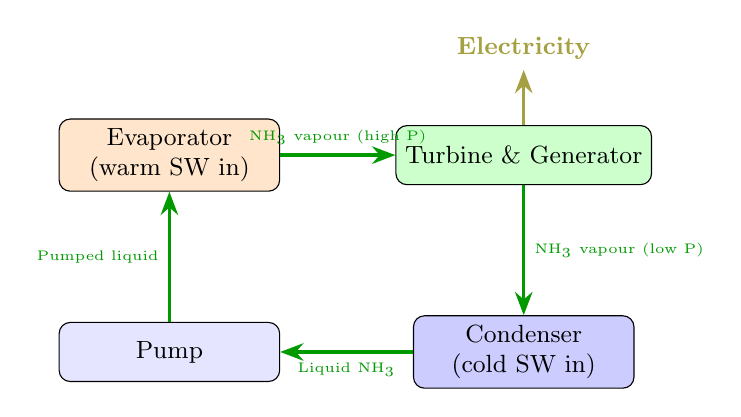
\begin{tikzpicture}[
  comp/.style={draw,fill=blue!10,rounded corners,minimum width=2.8cm,
               minimum height=0.75cm,align=center,font=\small},
  arr/.style={-Stealth,thick}]
  \node[comp,fill=orange!20] (E) at (0,0)    {Evaporator\\(warm SW in)};
  \node[comp,fill=green!20]  (T) at (4.5,0)  {Turbine \& Generator};
  \node[comp,fill=blue!20]   (C) at (4.5,-2.5){Condenser\\(cold SW in)};
  \node[comp]                (P) at (0,-2.5)  {Pump};

  \draw[arr,green!60!black,line width=1.2pt] (E.east) -- node[above,font=\tiny]{NH$_3$ vapour (high P)} (T.west);
  \draw[arr,green!60!black,line width=1.2pt] (T.south)-- node[right,font=\tiny]{NH$_3$ vapour (low P)} (C.north);
  \draw[arr,green!60!black,line width=1.2pt] (C.west) -- node[below,font=\tiny]{Liquid NH$_3$} (P.east);
  \draw[arr,green!60!black,line width=1.2pt] (P.north)-- node[left,font=\tiny]{Pumped liquid} (E.south);
  \draw[-Stealth,thick,yellow!60!black,line width=1.2pt] (T.north)--++(0,0.7) node[above,font=\small]{\textbf{Electricity}};
\end{tikzpicture}
\end{center}

\begin{itemize}[leftmargin=1.5em,itemsep=1pt]
  \item Warm seawater ($\sim$27\,°C) evaporates ammonia $\to$ vapour drives turbine-generator.
  \item Cold deep seawater ($\sim$5\,°C, depth $>$800\,m) condenses vapour back to liquid.
  \item Thermodynamic efficiency: $\eta_{\text{actual}} \approx 3$--5\% (low $\Delta T$), but fuel cost = zero.
  \item \textbf{Key advantage:} 24-hour continuous output, unlike solar/wind.
\end{itemize}

\hrulefill

\textbf{(ii) Hydroelectric Energy}

\textbf{Principle:} $P = \eta\,\rho\,g\,Q\,h$. See Q1(a) for full sketch and component description.

\textbf{Energy conversion flowchart:}

\begin{center}
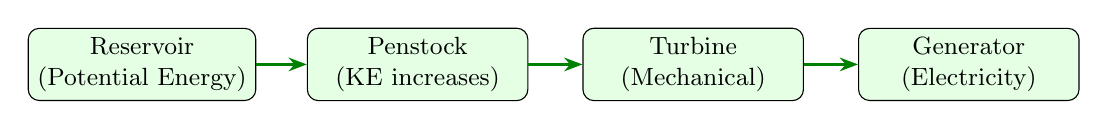
\begin{tikzpicture}[
  block/.style={draw,fill=green!10,rounded corners,minimum width=2.8cm,
                minimum height=0.65cm,align=center,font=\small},
  arr/.style={-Stealth,thick,green!50!black}]
  \node[block] (R) at (0,0)   {Reservoir\\(Potential Energy)};
  \node[block] (P) at (3.5,0) {Penstock\\(KE increases)};
  \node[block] (T) at (7,0)   {Turbine\\(Mechanical)};
  \node[block] (G) at (10.5,0){Generator\\(Electricity)};
  \draw[arr] (R)--(P); \draw[arr] (P)--(T); \draw[arr] (T)--(G);
\end{tikzpicture}
\end{center}

Key facts: $\sim$20\% of world electricity is from hydro; Kaptai HPP (Bangladesh) = 230\,MW; Three Gorges (China) = 22,500\,MW.

\end{tcolorbox}

% ── Q6 ────────────────────────────────────────────────────────
\item \label{qlabel:A1-Q4}
(a) Mention the key challenges in the energy sector of Bangladesh. What are your recommendations to tackle those challenges? \mk{8}\\
(b) Write short notes on any \textbf{three}: (i) OTEC, (ii) Wind turbine, (iii) Geothermal energy, (iv) Pressurised water nuclear reactor, (v) Bio-diesel. \mk{15}
\yr{2017--18}

\begin{tcolorbox}[enhanced,breakable,ansbox,colback=cA!4,colframe=cA,
  boxrule=0.8pt,arc=5pt,
  title={\textbf{Answer}},fonttitle=\bfseries\color{white},colbacktitle=cA]

\textbf{Part (a): Energy Sector Challenges and Recommendations}

\begin{center}
\small
\begin{tabular}{@{}p{6.2cm}p{7.3cm}@{}}
\toprule
\textbf{Challenge} & \textbf{Recommendation} \\
\midrule
Heavy dependence on imported LNG and fossil fuels & Accelerate domestic renewable deployment (solar, wind, biomass) \\[4pt]
Frequent load-shedding due to supply-demand gap & Invest in grid infrastructure and demand-side management \\[4pt]
Ageing, low-efficiency power plants & Replace with high-efficiency combined-cycle gas turbines \\[4pt]
High system losses ($\sim$10\%) in T\&D & Upgrade grid; reduce technical and non-technical losses \\[4pt]
No large-scale energy storage & Promote pumped hydro and battery storage \\[4pt]
Limited skilled workforce in renewable energy & Establish training institutes; include RE in engineering curricula \\
\bottomrule
\end{tabular}
\end{center}

\hrulefill

\textbf{Part (b): Short Notes (three)}

\medskip
\textbf{(i) OTEC} — see Q1(b)(i). Uses ocean temperature gradient for closed Rankine cycle with ammonia; 24/7 output.

\medskip
\textbf{(ii) Wind Turbine}

A wind turbine converts the \emph{kinetic energy of wind} into electrical energy.
\[
  P_{\text{available}} = \frac{1}{2}\,\rho_{\text{air}}\,A\,v^3
  \qquad \text{where } A = \pi R^2,\quad \rho_{\text{air}} \approx 1.225\,\text{kg/m}^3
\]

\begin{itemize}[leftmargin=1.5em,itemsep=2pt]
  \item \textbf{HAWT (Horizontal Axis):} Most common; blades rotate about horizontal axis facing the wind; high efficiency.
  \item \textbf{VAWT (Vertical Axis):} Works with wind from any direction; lower efficiency; simpler maintenance.
  \item \textbf{Betz Limit:} Maximum theoretical efficiency = 59.3\%; modern HAWTs achieve $\sim$45\%.
  \item Also used as \textbf{windmills} (grinding grain) and \textbf{windpumps} (pumping water).
\end{itemize}

\medskip
\textbf{(iii) Geothermal Energy} — see Q1(b)(iv). Three plant types: Dry Steam, Flash Steam, Binary Cycle. Baseload 24/7 power; $>$11,000\,MW worldwide.

\medskip
\textbf{(v) Bio-diesel}
\begin{itemize}[leftmargin=1.5em,itemsep=2pt]
  \item Renewable liquid fuel produced from vegetable oils / animal fats / recycled cooking oil via \textbf{transesterification} with methanol (NaOH catalyst):
  \[
    \text{Triglyceride} + 3\,\text{CH}_3\text{OH}
    \;\xrightarrow{\text{NaOH}}\;
    \text{Glycerol} + 3\,\text{FAME (biodiesel)}
  \]
  \item Blended as B20 (20\% biodiesel + 80\% diesel) or used pure (B100).
  \item \textbf{Advantages:} Renewable; lower net CO$_2$; biodegradable; higher flash point.
  \item \textbf{Disadvantages:} Competes with food crops; slightly lower energy density than diesel.
\end{itemize}

\end{tcolorbox}

% ── Q5 ────────────────────────────────────────────────────────
\item \label{qlabel:A1-Q3}
(a) What are the potential renewable energy sources in Bangladesh? Discuss the challenges and future prospects of renewable energy in Bangladesh. \mk{15}\\
(b) Write short notes on any \textbf{four}: (i) Solar photovoltaic cell, (ii) Pressurised water nuclear reactor, (iii) Ocean thermal energy conversion (OTEC), (iv) Pumped hydro storage system, (v) CETO technology. \mk{20}
\yr{2016--17}

\begin{tcolorbox}[enhanced,breakable,ansbox,colback=cA!4,colframe=cA,
  boxrule=0.8pt,arc=5pt,
  title={\textbf{Answer}},fonttitle=\bfseries\color{white},colbacktitle=cA]

\textbf{Part (a): Renewable Energy in Bangladesh}

\textbf{Potential Sources:}
\begin{itemize}[leftmargin=1.5em,itemsep=2pt]
  \item \textbf{Solar:} Bangladesh receives $\sim$4--5\,kWh/m²/day; $>$4 million Solar Home Systems already deployed; grid-scale solar parks expanding.
  \item \textbf{Biomass:} Agricultural residues (rice husk, bagasse, jute sticks), biogas from animal dung, municipal solid waste.
  \item \textbf{Wind:} Coastal belt (Kutubdia, Cox's Bazar, Feni) with average wind speeds of 4--6\,m/s; offshore potential in Bay of Bengal.
  \item \textbf{Hydropower:} Kaptai HPP (230\,MW) on Karnaphuli River — currently the only hydro plant.
  \item \textbf{Tidal:} Long Bay of Bengal coastline with tidal ranges of 2--5\,m offers future potential.
\end{itemize}

\textbf{Challenges:}
\begin{itemize}[leftmargin=1.5em,itemsep=2pt]
  \item High capital cost relative to the national GDP.
  \item Intermittency of solar and wind with no large-scale storage infrastructure.
  \item Limited land area for utility-scale solar and wind farms.
  \item Weak grid infrastructure in rural areas.
  \item Shortage of skilled manpower for installation and maintenance.
  \item Policy and financing barriers for private sector investment.
\end{itemize}

\textbf{Future Prospects:}
\begin{itemize}[leftmargin=1.5em,itemsep=2pt]
  \item Government target: 40\% renewable energy by 2041 (Mujib Climate Prosperity Plan).
  \item Rapidly falling global solar PV costs ($>$90\% reduction since 2010).
  \item Floating solar on haors and irrigation canals — innovative land-saving approach.
  \item Offshore wind development in the Bay of Bengal.
  \item International climate finance (Green Climate Fund) to support the energy transition.
\end{itemize}

\hrulefill

\textbf{Part (b): Short Notes (four)}

\medskip
\textbf{(i) Solar Photovoltaic Cell} — see Q1(b)(ii) for detailed mechanism.

A p-n junction of doped silicon converts photons $\to$ electron flow (DC current) via the photoelectric effect. System: Cells $\to$ Module $\to$ Array $\to$ Inverter $\to$ Grid. Efficiency: 15--22\%; lifetime $>$30 years; no emissions during operation.

\medskip
\textbf{(ii) Pressurised Water Reactor (PWR)}
\begin{itemize}[leftmargin=1.5em,itemsep=2pt]
  \item \textbf{Fuel:} Low-enriched ${}^{235}$U (3--5\%).
  \item \textbf{Primary loop:} Water maintained at $\sim$155\,bar; does not boil even at 320\,°C; acts as both \emph{coolant} and \emph{moderator}.
  \item \textbf{Secondary loop:} Heat exchanged via steam generator $\to$ steam drives turbine $\to$ generator produces electricity. Radioactive primary water never contacts the turbine.
  \item \textbf{Safety:} Negative temperature coefficient — fission rate self-limits if coolant heats up.
  \item Bangladesh's Rooppur NPP (2$\times$1200\,MW) is a modern PWR (VVER-1200).
\end{itemize}

\medskip
\textbf{(iii) OTEC} — see Q1(b)(i) for detailed note.

Uses ocean temperature gradient (surface warm vs.\ deep cold) for a closed Rankine cycle with ammonia as working fluid. Produces electricity 24/7, independent of weather.

\medskip
\textbf{(iv) Pumped Hydro Storage System}
\begin{itemize}[leftmargin=1.5em,itemsep=2pt]
  \item World's largest form of grid-scale energy storage ($>$90\% of global storage capacity).
  \item \textbf{Charging (off-peak):} Surplus electricity pumps water from lower $\to$ upper reservoir, storing gravitational potential energy: $E = \rho\,V\,g\,h$.
  \item \textbf{Discharging (peak):} Water flows back down through turbines $\to$ generates electricity.
  \item Round-trip efficiency: 70--85\%.
  \item Ideal partner for intermittent renewables (solar, wind).
\end{itemize}

\medskip
\textbf{(v) CETO Technology}
\begin{itemize}[leftmargin=1.5em,itemsep=2pt]
  \item Fully \emph{submerged} wave energy technology developed by Carnegie Clean Energy (Australia); named after the Greek sea goddess Ceto.
  \item \textbf{Principle:} Buoys moored to the seabed move with waves $\to$ drive seabed-mounted pumps $\to$ pressurised seawater drives onshore turbines (electricity) and can simultaneously power reverse-osmosis desalination.
  \item \textbf{Advantage:} Fully submerged (invisible, storm-protected); dual output: power + fresh water.
  \item Currently in demonstration/early-commercial phase.
\end{itemize}

\end{tcolorbox}

% ── Q4 ────────────────────────────────────────────────────────
\item \label{qlabel:A1-Q14}
Define renewable energy and give examples. With suitable diagrams or flowcharts, write short notes on: (i) Nuclear-energy-powered Pressurised Water Reactor, (ii) Geothermal Energy. \mk{20}
\yr{2015--16}

\begin{tcolorbox}[enhanced,breakable,ansbox,colback=cA!4,colframe=cA,
  boxrule=0.8pt,arc=5pt,
  title={\textbf{Answer}},fonttitle=\bfseries\color{white},colbacktitle=cA]

\textbf{Renewable Energy:} Energy from sources naturally replenished on human timescales.\\
\textbf{Examples:} Solar, wind, hydro, tidal, OTEC, geothermal, biomass, wave.

\hrulefill

\textbf{(i) Pressurised Water Reactor (PWR)}

\textbf{Working Principle:}

\begin{center}
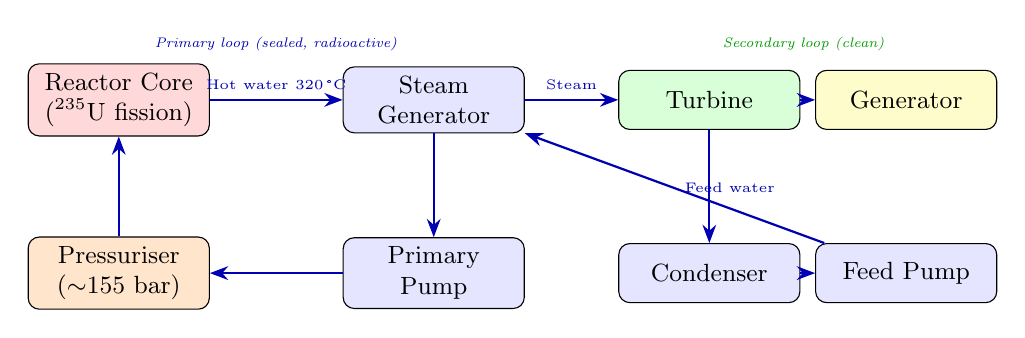
\begin{tikzpicture}[
  block/.style={draw,rounded corners,minimum width=2.3cm,minimum height=0.75cm,
                align=center,font=\small,fill=blue!10},
  arr/.style={-Stealth,thick,blue!70!black}]

  \node[block,fill=red!15]   (core) at (0,0)    {Reactor Core\\(${}^{235}$U fission)};
  \node[block]               (sg)   at (4,0)    {Steam\\Generator};
  \node[block,fill=orange!20](pres) at (0,-2.2) {Pressuriser\\($\sim$155 bar)};
  \node[block]               (pp)   at (4,-2.2) {Primary\\Pump};

  \draw[arr] (core)--node[above,font=\tiny]{Hot water 320\,°C}(sg);
  \draw[arr] (sg)--(pp); \draw[arr] (pp)--(pres); \draw[arr] (pres)--(core);

  \node[block,fill=green!15] (turb) at (7.5,0)  {Turbine};
  \node[block,fill=yellow!20](gen)  at (10,0)   {Generator};
  \node[block]               (cond) at (7.5,-2.2){Condenser};
  \node[block]               (fp)   at (10,-2.2) {Feed Pump};

  \draw[arr] (sg)--node[above,font=\tiny]{Steam}(turb);
  \draw[arr] (turb)--(gen);
  \draw[arr] (turb)--(cond);
  \draw[arr] (cond)--(fp);
  \draw[arr] (fp)--node[right,font=\tiny]{Feed water}(sg);

  \node[font=\tiny,text=blue!70!black,above] at (2,0.5) {\textit{Primary loop (sealed, radioactive)}};
  \node[font=\tiny,text=green!60!black,above] at (8.7,0.5) {\textit{Secondary loop (clean)}};
\end{tikzpicture}
\end{center}

\begin{itemize}[leftmargin=1.5em,itemsep=2pt]
  \item \textbf{Fuel:} Low-enriched ${}^{235}$U (3--5\%).
  \item \textbf{Primary loop:} Water at $\sim$155\,bar; stays liquid at 320\,°C; acts as coolant \emph{and} moderator.
  \item \textbf{Secondary loop:} Clean steam generated in steam generator drives turbine. Radioactive water never contacts the turbine.
  \item \textbf{Safety:} Negative temperature coefficient — fission auto-limits if temperature rises. Multiple passive safety barriers.
  \item Thermal efficiency $\approx$33\%. Bangladesh's Rooppur NPP (2$\times$1200\,MW) is a modern PWR.
\end{itemize}

\hrulefill

\textbf{(ii) Geothermal Energy} — see Q12 for full description.

\textbf{Flowchart:}

\begin{center}
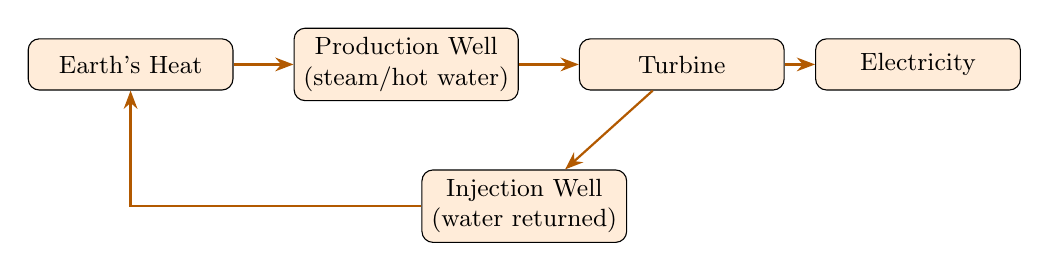
\begin{tikzpicture}[
  block/.style={draw,fill=orange!15,rounded corners,minimum width=2.6cm,
                minimum height=0.65cm,align=center,font=\small},
  arr/.style={-Stealth,thick,orange!70!black}]
  \node[block](E) at (0,0)  {Earth's Heat};
  \node[block](W) at (3.5,0){Production Well\\(steam/hot water)};
  \node[block](T) at (7,0)  {Turbine};
  \node[block](G) at (10,0) {Electricity};
  \node[block](I) at (5,-1.8){Injection Well\\(water returned)};
  \draw[arr](E)--(W); \draw[arr](W)--(T); \draw[arr](T)--(G);
  \draw[arr](T)--(I); \draw[arr](I)--++(-5,0)--(E);
\end{tikzpicture}
\end{center}


\begin{center}
  
\includegraphics[width=0.3\textwidth,keepaspectratio]{/A14a.png}
  
\includegraphics[height=0.3\textheight,width=0.3\textwidth,keepaspectratio]{/A14b.png}
  
\includegraphics[height=0.3\textheight,width=0.3\textwidth,keepaspectratio]{/A14c.png}
\end{center}

\end{tcolorbox}

% ── Q15 ────────────────────────────────────────────────────────
\item \label{qlabel:A1-Q13}
Write down the names of potential sources of renewable energy and briefly describe solar thermal energy. \mk{10}
\yr{2014--15}

\begin{tcolorbox}[enhanced,breakable,ansbox,colback=cA!4,colframe=cA,
  boxrule=0.8pt,arc=5pt,
  title={\textbf{Answer}},fonttitle=\bfseries\color{white},colbacktitle=cA]

\textbf{Renewable Energy Sources:} Solar, Wind, Hydroelectric, Tidal, OTEC, Geothermal, Biomass, Wave.

\hrulefill

\textbf{Solar Thermal Energy}

Solar thermal systems utilise the \emph{heat} in solar radiation (as opposed to PV which uses the photoelectric effect).

\textbf{Application 1 — Concentrating Solar Power (CSP) for electricity:}
\begin{itemize}[leftmargin=1.5em,itemsep=2pt]
  \item \textbf{Step 1 — Concentration:}
    \begin{itemize}[leftmargin=1.5em]
      \item \emph{Parabolic trough:} Linear-focus curved mirrors heat transfer fluid in receiver tube to $\sim$390\,°C.
      \item \emph{Solar power tower:} Field of heliostats focuses onto central tower receiver; temperatures $>$500\,°C; optional molten-salt thermal storage.
    \end{itemize}
  \item \textbf{Step 2:} Heat $\to$ steam generator $\to$ high-pressure steam.
  \item \textbf{Step 3:} Steam $\to$ turbine $\to$ generator $\to$ electricity.
\end{itemize}

\textbf{Application 2 — Solar Water and Space Heating:}
\begin{itemize}[leftmargin=1.5em,itemsep=1pt]
  \item Flat-plate or evacuated-tube \emph{solar collectors} on rooftops heat domestic water. Cold water circulates through collector; hot water rises to storage tank (thermosiphon).
  \item \emph{Passive solar heating:} South-facing glazing, thermal mass walls, insulated roof to capture and store solar heat without any active equipment.
\end{itemize}

\[
  \text{Solar radiation} \;\xrightarrow{\text{mirrors/collector}}\; \text{High-temp fluid/water}
  \;\xrightarrow{\text{turbine or direct use}}\; \text{Electricity / Heat}
\]

\end{tcolorbox}

% ── Q14 ────────────────────────────────────────────────────────
\item \label{qlabel:A1-Q12}
Write down the potential sources of renewable energy and briefly explain geothermal energy. \mk{12}
\yr{2013--14}

\begin{tcolorbox}[enhanced,breakable,ansbox,colback=cA!4,colframe=cA,
  boxrule=0.8pt,arc=5pt,
  title={\textbf{Answer}},fonttitle=\bfseries\color{white},colbacktitle=cA]

\textbf{Potential Renewable Energy Sources:}

Solar energy (thermal \& PV), Wind energy, Hydroelectric power, Tidal energy, Ocean Thermal Energy (OTEC), Geothermal energy, Biomass \& biodiesel, Wave energy.

\hrulefill

\textbf{Geothermal Energy}

\textbf{Source:} Natural heat of the Earth's interior. Core $\approx$6000\,°C; temperature rises $\approx$1\,°C per 36\,m depth. In volcanic regions, molten rock (magma) is close to the surface.

\textbf{Extraction:} Hot water or steam extracted from underground reservoirs through production wells; spent water returned via injection wells to sustain the resource.

\textbf{Three plant designs:}
\begin{enumerate}[leftmargin=2em,itemsep=2pt]
  \item \textbf{Dry Steam Plant:} Steam from well $\to$ directly drives turbine $\to$ condenser. Used where steam is directly available.
  \item \textbf{Flash Steam Plant:} Very hot pressurised water is depressurised (``flashed'') into steam $\to$ drives turbine. Used with very hot water ($>$180\,°C).
  \item \textbf{Binary Cycle Plant:} Hot water heats a secondary low-boiling fluid (isobutane) in a heat exchanger; isobutane vapour drives turbine. Most versatile — works with lower temperature water; currently the most widely built new type.
\end{enumerate}

$>$11,000\,MW installed worldwide. 24/7 baseload power; zero fuel cost; minimal emissions. Widely used in Iceland, USA, Kenya, Philippines.

\end{tcolorbox}

% ── Q13 ────────────────────────────────────────────────────────
\item \label{qlabel:A1-Q8}
Define renewable energy and list the potential sources of renewable and non-renewable energy. \mk{10}
\yr{2012--13}

\begin{tcolorbox}[enhanced,breakable,ansbox,colback=cA!4,colframe=cA,
  boxrule=0.8pt,arc=5pt,
  title={\textbf{Answer}},fonttitle=\bfseries\color{white},colbacktitle=cA]

\textbf{Definition:} Renewable energy sources are those that are \emph{naturally replenishing} on human timescales — they do not deplete with use and are continuously regenerated by natural processes.

\begin{center}
\small
\begin{tabular}{@{}p{7cm}p{7cm}@{}}
\toprule
\textbf{Renewable Sources} & \textbf{Non-Renewable (Conventional) Sources} \\
\midrule
Solar energy (thermal \& PV)   & Coal \\
Wind energy                    & Petroleum (crude oil) \\
Hydroelectric power            & Natural gas \\
Tidal energy                   & Nuclear (${}^{235}$U, ${}^{239}$Pu) \\
Ocean thermal energy (OTEC)    & Liquefied petroleum gas (LPG) \\
Geothermal energy              & Compressed natural gas (CNG) \\
Biomass and biodiesel          & Oil shale and tar sands \\
Wave energy                    & \\
\bottomrule
\end{tabular}
\end{center}

\textbf{Key distinction:} Non-renewable sources took millions of years to form and are consumed far faster than they regenerate. Renewable sources are replenished by natural cycles (solar radiation, water cycle, wind, tides) within human timescales.

\end{tcolorbox}

% ── Q9 ────────────────────────────────────────────────────────
\item \label{qlabel:A1-Q9}
(a) What is fossil fuel? What are its forms? How long are current reserves expected to last? \mk{10}\\
(b) What is renewable energy? What renewable sources are used for electric power generation in Bangladesh? \mk{8}\\
(c) Why are biomasses (wood, leaf, rice husk, etc.) considered renewable? \mk{7}
\yr{2011--12}

\begin{tcolorbox}[enhanced,breakable,ansbox,colback=cA!4,colframe=cA,
  boxrule=0.8pt,arc=5pt,
  title={\textbf{Answer}},fonttitle=\bfseries\color{white},colbacktitle=cA]

\textbf{Part (a): Fossil Fuels}

\textbf{Definition:} Fossil fuels are energy-rich carbon compounds formed from the \emph{fossilised remains of dead plants and animals} buried under the Earth's surface and subjected to intense heat and pressure over hundreds of millions of years.

\textbf{Forms:}
\begin{itemize}[leftmargin=1.5em,itemsep=2pt]
  \item \textbf{Coal (solid):} Highest carbon content; extracted by strip mining or deep tunnelling.
  \item \textbf{Petroleum / Crude Oil (liquid):} Found deep underground; extracted by drilling and pump jacks.
  \item \textbf{Natural Gas (gaseous):} Mainly CH$_4$; often co-located with oil; transported via pipelines.
\end{itemize}

\textbf{Estimated Remaining Reserves (at current consumption rates):}
\begin{center}
\small
\begin{tabular}{@{}lc@{}}
\toprule
\textbf{Fuel} & \textbf{Approx.\ reserves remaining} \\
\midrule
Coal         & $\sim$130 years \\
Natural gas  & $\sim$50--60 years \\
Petroleum    & $\sim$50 years \\
\bottomrule
\end{tabular}
\end{center}

\hrulefill

\textbf{Part (b): Renewable Energy — Bangladesh's Sources}

Definition: See Q8. Renewable sources currently used for electricity in Bangladesh:
\begin{itemize}[leftmargin=1.5em,itemsep=1pt]
  \item \textbf{Hydropower:} Kaptai HPP (230\,MW) on the Karnaphuli River.
  \item \textbf{Solar PV:} $>$4 million Solar Home Systems; grid-scale solar parks (e.g.\ Teknaf 28\,MW).
  \item \textbf{Biomass/Biogas:} Small-scale biogas digesters; rice husk gasifiers.
  \item \textbf{Wind:} Small pilots in coastal areas (Kutubdia, Feni).
\end{itemize}

\hrulefill

\textbf{Part (c): Why Biomass is Considered Renewable}

\begin{itemize}[leftmargin=1.5em,itemsep=2pt]
  \item Plants absorb CO$_2$ during \emph{photosynthesis} to grow. When burned, that same CO$_2$ is released — making the net carbon cycle \textbf{approximately carbon-neutral}.
  \item Crops and forests can be \emph{regrown} within years to decades, not millions of years.
  \item As long as harvest rate $\leq$ regrowth rate, the resource is \emph{sustainable}.
\end{itemize}

\[
  \underbrace{\text{CO}_2 + \text{H}_2\text{O} \xrightarrow{\text{sunlight}} \text{Biomass} + \text{O}_2}_{\text{photosynthesis (growth)}}
  \qquad
  \underbrace{\text{Biomass} + \text{O}_2 \to \text{CO}_2 + \text{H}_2\text{O} + \text{Heat}}_{\text{combustion (energy release)}}
\]

The cycle is closed — unlike fossil fuels where carbon was locked away for millions of years.

\end{tcolorbox}

% ── Q10 ────────────────────────────────────────────────────────
\item \label{qlabel:A1-Q10}
(a) Discuss the various concepts of extracting solar energy. \mk{10}\\
(b) Describe briefly the extraction method of crude oil. \mk{10}
\yr{2010--11}

\begin{tcolorbox}[enhanced,breakable,ansbox,colback=cA!4,colframe=cA,
  boxrule=0.8pt,arc=5pt,
  title={\textbf{Answer}},fonttitle=\bfseries\color{white},colbacktitle=cA]

\textbf{Part (a): Concepts of Extracting Solar Energy}

Solar constant = 1352\,W/m²; $\sim$50\% reaches Earth's surface (21\% direct + 29\% diffuse).

\textbf{1.\ Solar Thermal Energy:}

\textit{(A) Concentrating Solar Power (CSP) for electricity:}
\begin{itemize}[leftmargin=1.5em,itemsep=1pt]
  \item \textbf{Parabolic trough:} Curved mirrors focus sun onto receiver tube; HTF heated to $\sim$390\,°C $\to$ steam $\to$ turbine.
  \item \textbf{Solar power tower:} Array of heliostats focuses onto central receiver atop tower; temperatures $>$500\,°C; molten salt storage enables post-sunset generation.
\end{itemize}

\textit{(B) Water and space heating:}
\begin{itemize}[leftmargin=1.5em,itemsep=1pt]
  \item Flat-plate or evacuated-tube collectors heat domestic water.
  \item Passive solar building design uses thermal mass and south-facing glazing.
\end{itemize}

\textbf{2.\ Solar Photovoltaic (PV):}
\begin{itemize}[leftmargin=1.5em,itemsep=1pt]
  \item Semiconductor p-n junction converts photons $\to$ DC electricity via photoelectric effect.
  \item No moving parts; scalable from milliwatts to gigawatts.
\end{itemize}

\begin{center}
\small
\begin{tabular}{@{}lll@{}}
\toprule
\textbf{Method} & \textbf{Output} & \textbf{Best Scale} \\
\midrule
CSP (parabolic/tower) & Heat / Electricity & Utility (MW--GW) \\
Solar PV              & DC Electricity     & All scales \\
Solar water heater    & Heat               & Residential / commercial \\
\bottomrule
\end{tabular}
\end{center}

\hrulefill

\textbf{Part (b): Extraction of Crude Oil}

\begin{itemize}[leftmargin=1.5em,itemsep=2pt]
  \item \textbf{Exploration:} Seismic surveys and imaging technology identify oil-bearing geological formations (anticlines, fault traps).
  \item \textbf{Drilling:} Rotary drill bit cuts through rock. Drilling mud circulates to cool the bit, carry cuttings to surface, and control pressure.
  \item \textbf{On land:} A \emph{derrick} supports the drill string. After striking oil, a \emph{pump jack} lifts oil if natural pressure is insufficient.
  \item \textbf{Offshore:} Massive \emph{oil platforms} (fixed or floating) with subsea wellheads and risers.
  \item \textbf{Primary recovery:} Natural reservoir pressure drives oil to surface.
  \item \textbf{Secondary recovery:} Water or gas injection maintains pressure as reservoir depletes.
  \item \textbf{Tertiary (EOR):} Steam injection, chemical flooding, or CO$_2$ injection to mobilise remaining oil.
  \item Natural gas is often co-located and captured from the same reservoirs.
\end{itemize}

\end{tcolorbox}

% ── Q11 ────────────────────────────────────────────────────────
\item \label{qlabel:A1-Q11}
(a) What are the localised environmental concerns of air pollution? \mk{7}\\
(b) What do you know about LPG and CNG? \mk{8}
\yr{2010--11}

\begin{tcolorbox}[enhanced,breakable,ansbox,colback=cA!4,colframe=cA,
  boxrule=0.8pt,arc=5pt,
  title={\textbf{Answer}},fonttitle=\bfseries\color{white},colbacktitle=cA]

\textbf{Part (a): Localised Environmental Concerns of Air Pollution}

\begin{itemize}[leftmargin=1.5em,itemsep=2pt]
  \item \textbf{Smog:} Ground-level O$_3$ from NOx + VOCs in sunlight; reduces visibility; damages lung tissue.
  \item \textbf{Acid Rain:} SO$_2$ + NOx dissolve in moisture $\to$ H$_2$SO$_4$ + HNO$_3$; kills forests; acidifies lakes; corrodes limestone buildings.
  \item \textbf{Particulate Matter (PM$_{2.5}$, PM$_{10}$):} Fine particles penetrate deep into lungs; cause respiratory and cardiovascular disease.
  \item \textbf{Carbon Monoxide (CO):} From incomplete combustion; binds haemoglobin; prevents oxygen transport; toxic.
  \item \textbf{Reduced crop yields:} Ground-level ozone and acid deposition damage vegetation and soil near industrial areas.
  \item \textbf{Eutrophication:} Nitrogen deposition from NOx promotes algal blooms in nearby water bodies, depleting oxygen.
\end{itemize}

\hrulefill

\textbf{Part (b): LPG and CNG}

\textbf{LPG — Liquefied Petroleum Gas:}
\begin{itemize}[leftmargin=1.5em,itemsep=1pt]
  \item Mixture of \textbf{propane} (C$_3$H$_8$) and \textbf{butane} (C$_4$H$_{10}$); by-product of oil refining / gas processing.
  \item Stored as \emph{liquid} under moderate pressure ($\sim$7--10\,bar); returns to gas at atmospheric pressure.
  \item Uses: cooking, heating, automotive fuel. Calorific value $\approx$ 46--50\,MJ/kg.
  \item \textbf{Hazard:} Denser than air — leaks collect at floor level, explosion risk.
\end{itemize}

\textbf{CNG — Compressed Natural Gas:}
\begin{itemize}[leftmargin=1.5em,itemsep=1pt]
  \item Mainly \textbf{methane} (CH$_4$, $>$90\%); compressed to $\sim$200--250\,bar in high-pressure cylinders.
  \item Uses: vehicle fuel (buses, cars, rickshaws), piped domestic supply. Calorific value $\approx$ 50--55\,MJ/kg.
  \item Lighter than air — safer than LPG in case of leak (disperses upward).
  \item Significantly lower CO$_2$, CO, and particulate emissions than petrol/diesel.
\end{itemize}

\begin{center}
\small
\begin{tabular}{@{}llll@{}}
\toprule
\textbf{Property} & \textbf{LPG} & \textbf{CNG} \\
\midrule
Main component & Propane/Butane (C$_3$--C$_4$) & Methane (CH$_4$) \\
Storage state  & Liquid (moderate pressure)    & Gas ($\sim$200\,bar) \\
Density vs air & Heavier                       & Lighter \\
Primary use    & Cooking, heating              & Vehicles, domestic \\
\bottomrule
\end{tabular}
\end{center}

\end{tcolorbox}

% ── Q12 ────────────────────────────────────────────────────────
\item \label{qlabel:A1-Q15}
(a) State the criteria of a source of energy. Hence explain that nuclear energy qualifies as one. \mk{12}\\
(b) Write a short note on Photovoltaic Cell. \mk{9}
\yr{2008--09}

\begin{tcolorbox}[enhanced,breakable,ansbox,colback=cA!4,colframe=cA,
  boxrule=0.8pt,arc=5pt,
  title={\textbf{Answer}},fonttitle=\bfseries\color{white},colbacktitle=cA]

\textbf{Part (a): Criteria and Nuclear Energy}

\textbf{Criteria for a viable energy source:}
\begin{enumerate}[leftmargin=2em,itemsep=2pt]
  \item \textbf{Availability:} Obtainable in adequate quantities.
  \item \textbf{Storability:} Capable of being stored for on-demand use.
  \item \textbf{Transportability:} Can be moved from source to point of use.
  \item \textbf{Convertibility:} Convertible to useful forms (heat, electricity, mechanical work).
  \item \textbf{Economic viability:} Cost of extraction and conversion must be acceptable.
  \item \textbf{Safety:} Risks during handling and use must be manageable.
\end{enumerate}

\textbf{Nuclear energy satisfies all criteria:}

\begin{center}
\small
\begin{tabular}{@{}lp{10cm}@{}}
\toprule
\textbf{Criterion} & \textbf{How nuclear energy satisfies it} \\
\midrule
Availability    & Uranium reserves $>$100 years; thorium and Pu-239 breeding extend this further \\
Storability     & Fuel pellets stored safely for years; 1\,cm pellet $\equiv$ 1 tonne of coal \\
Transportability& Compact fuel assemblies transported worldwide in shielded casks \\
Convertibility  & Fission $\to$ heat $\to$ steam $\to$ turbine $\to$ electricity; $\eta\approx 33\%$ \\
Economic viability & High capital cost but very low fuel cost; capacity factor $\sim$90\% \\
Safety          & Multiple passive safety systems; lowest deaths-per-kWh of any energy source \\
\bottomrule
\end{tabular}
\end{center}

\[
  \boxed{E = \Delta m\cdot c^2 \approx 200\,\text{MeV per fission of }{}^{235}\text{U}}
\]

\hrulefill

\textbf{Part (b): Photovoltaic Cell} — see Q1(b)(ii) for detailed note.

A p-n junction of doped silicon converts photons $\to$ DC current via photoelectric effect.
\begin{itemize}[leftmargin=1.5em,itemsep=1pt]
  \item \textbf{n-type layer:} Electron-rich; \textbf{p-type layer:} Hole-rich; built-in field at junction sweeps carriers apart.
  \item Freed electrons flow through external circuit $\to$ DC current.
  \item Efficiency: 15--22\% (commercial); lifetime $>$30 years; no moving parts.
  \item System: Cells $\to$ Module $\to$ Array $\to$ Inverter (DC$\to$AC) $\to$ Grid.
\end{itemize}

\end{tcolorbox}

% ── Q16 ────────────────────────────────────────────────────────
\item \label{qlabel:A1-Q16}
(a) What environmental hazards are associated with burning fossil fuels? \mk{10}\\
(b) Write short notes on: (i) Geothermal Energy, (ii) Solar Energy. \mk{20}
\yr{2006--07}

\begin{tcolorbox}[enhanced,breakable,ansbox,colback=cA!4,colframe=cA,
  boxrule=0.8pt,arc=5pt,
  title={\textbf{Answer}},fonttitle=\bfseries\color{white},colbacktitle=cA]

\textbf{Part (a): Environmental Hazards of Burning Fossil Fuels}

\begin{center}
\small
\begin{tabular}{@{}p{2.5cm}p{4.5cm}p{6.5cm}@{}}
\toprule
\textbf{Pollutant} & \textbf{Source} & \textbf{Hazard} \\
\midrule
CO$_2$           & All fossil fuel combustion     & Greenhouse gas $\to$ global warming, climate change \\[3pt]
SO$_2$           & Coal and oil combustion        & Acid rain $\to$ forest damage, lake acidification, corrosion \\[3pt]
NOx              & High-temp.\ combustion         & Acid rain; smog; ground-level ozone; respiratory damage \\[3pt]
CO               & Incomplete combustion          & Toxic; binds haemoglobin; oxygen deprivation \\[3pt]
PM$_{2.5}$       & Coal; diesel engines           & Respiratory and cardiovascular disease \\[3pt]
CH$_4$ (leaks)   & Natural gas pipelines          & Potent GHG (28$\times$ CO$_2$ over 100 years) \\[3pt]
Heavy metals     & Coal combustion (Hg, Pb)       & Bioaccumulation; neurological damage \\
\bottomrule
\end{tabular}
\end{center}

\hrulefill

\textbf{Part (b): Short Notes}

\textbf{(i) Geothermal Energy} — see Q12 for full description.

Three plant types: Dry Steam, Flash Steam, Binary Cycle. $>$11,000\,MW worldwide; 24/7 baseload.

\medskip
\textbf{(ii) Solar Energy}

Sun generates energy via thermonuclear fusion; surface temperature $\sim$6000\,°C; solar constant = 1352\,W/m². Radiation spans visible, infrared, UV, X-ray, and radio.

\textbf{Two extraction methods:}
\begin{itemize}[leftmargin=1.5em,itemsep=2pt]
  \item \textbf{Solar Thermal (CSP):} Concentrating mirrors $\to$ high-temp fluid $\to$ steam $\to$ turbine $\to$ electricity. Also used for water and space heating. See Q13 for full description.
  \item \textbf{Solar PV:} Semiconductor p-n junction converts photons $\to$ DC electricity. See Q1(b)(ii) / Q15(b).
\end{itemize}

\emph{Key fact:} 30 days of sunshine on Earth contains the energy equivalent of all fossil fuel reserves ever used and remaining.

\end{tcolorbox}

% ── Q17 ────────────────────────────────────────────────────────
\item \label{qlabel:A1-Q17}
(a) What is meant by a renewable energy source? Give examples. \mk{5}\\
(b) Explain how steam can be produced from water using solar energy. \mk{10}\\
(c) What is OTEC? With a neat sketch, explain the closed-cycle OTEC system. \mk{15}
\yr{2005--06}

\begin{tcolorbox}[enhanced,breakable,ansbox,colback=cA!4,colframe=cA,
  boxrule=0.8pt,arc=5pt,
  title={\textbf{Answer}},fonttitle=\bfseries\color{white},colbacktitle=cA]

\textbf{Part (a):} See Q8. Examples: solar, wind, hydro, tidal, OTEC, geothermal, biomass, wave.

\hrulefill

\textbf{Part (b): Producing Steam from Water Using Solar Energy}

\textbf{Method 1 — Parabolic Trough CSP:}
\begin{itemize}[leftmargin=1.5em,itemsep=1pt]
  \item Parabolic mirrors track the sun; focus onto receiver tube at focal line.
  \item Heat transfer fluid (synthetic oil) heated to $\sim$390\,°C in the receiver.
  \item Hot fluid $\to$ steam generator (heat exchanger) $\to$ high-pressure steam.
  \item Steam $\to$ turbine $\to$ generator $\to$ electricity.
\end{itemize}

\textbf{Method 2 — Solar Power Tower (Heliostat):}
\begin{itemize}[leftmargin=1.5em,itemsep=1pt]
  \item Field of individually tracking flat mirrors (heliostats) reflects sunlight onto central receiver on tower.
  \item Receiver heats working fluid (water or molten salt) to $>$500\,°C.
  \item Molten salt stores thermal energy $\to$ steam production continues for hours after sunset.
\end{itemize}

\[
  \text{Solar radiation} \xrightarrow{\text{concentration}} \text{High-temp fluid}
  \xrightarrow{\text{heat exchanger}} \text{Steam}
  \xrightarrow{\text{turbine}} \text{Electricity}
\]

\hrulefill

\textbf{Part (c): OTEC — Closed-Cycle System}

\textbf{Definition:} OTEC uses the natural temperature difference ($\Delta T \approx 20$--25\,°C) between warm ocean surface water ($\sim$27\,°C) and cold deep seawater ($\sim$5\,°C, depth $>$800\,m) to run a thermodynamic cycle and generate electricity continuously.

\textbf{Neat sketch — Closed-Cycle OTEC:}

\begin{center}
  
\includegraphics[height=0.3\textheight,width=0.75\textwidth,keepaspectratio]{/A5.png}
\end{center}


\begin{center}
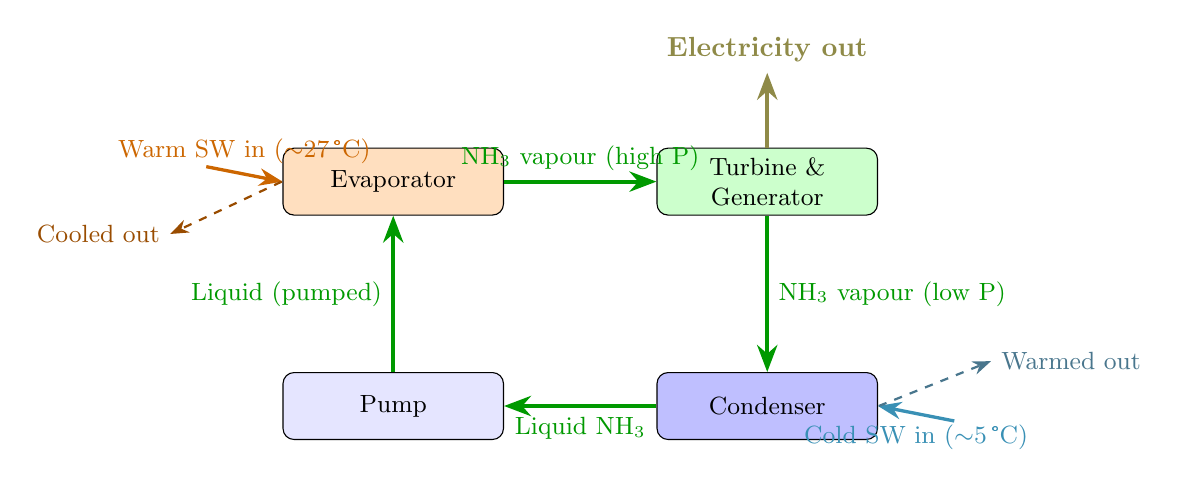
\begin{tikzpicture}[
  comp/.style={draw,fill=blue!10,rounded corners,minimum width=2.8cm,
               minimum height=0.85cm,align=center,font=\small},
  arr/.style={-Stealth,thick},
  scale=0.95]

  \node[comp,fill=orange!25] (evap) at (0,0)    {Evaporator};
  \node[comp,fill=green!20]  (turb) at (5,0)    {Turbine \&\\Generator};
  \node[comp,fill=blue!25]   (cond) at (5,-3)   {Condenser};
  \node[comp]                (pump) at (0,-3)   {Pump};

  % Working fluid loop
  \draw[arr,green!60!black,line width=1.5pt]
    (evap.east)--node[above,font=\small]{NH$_3$ vapour (high P)}(turb.west);
  \draw[arr,green!60!black,line width=1.5pt]
    (turb.south)--node[right,font=\small]{NH$_3$ vapour (low P)}(cond.north);
  \draw[arr,green!60!black,line width=1.5pt]
    (cond.west)--node[below,font=\small]{Liquid NH$_3$}(pump.east);
  \draw[arr,green!60!black,line width=1.5pt]
    (pump.north)--node[left,font=\small]{Liquid (pumped)}(evap.south);

  % Warm seawater
  \draw[arr,orange!80!black,line width=1.2pt]
    (-2.5,0.2)--node[above,font=\small]{Warm SW in ($\sim$27\,°C)}(evap.west);
  \draw[arr,orange!60!black,dashed]
    (evap.west)+(-0.01,0)--++(-1.5,-0.7)node[left,font=\small]{Cooled out};

  % Cold seawater
  \draw[arr,cyan!70!black,line width=1.2pt]
    (7.5,-3.2)--node[below,font=\small]{Cold SW in ($\sim$5\,°C)}(cond.east);
  \draw[arr,cyan!50!black,dashed]
    (cond.east)++(0.01,0)--++(1.5,0.6)node[right,font=\small]{Warmed out};

  % Electricity output
  \draw[-Stealth,yellow!50!black,line width=1.5pt]
    (turb.north)--++(0,1)node[above,font=\normalsize]{\textbf{Electricity out}};
\end{tikzpicture}
\end{center}

\textbf{Step-by-step:}
\begin{enumerate}[leftmargin=2em,itemsep=2pt]
  \item Warm surface seawater evaporates liquid ammonia (bp $= -33$\,°C) in the \emph{evaporator}.
  \item High-pressure NH$_3$ vapour expands through the \emph{turbine} $\to$ generator produces electricity.
  \item Low-pressure vapour enters \emph{condenser}; cold deep seawater ($\sim$5\,°C) condenses it to liquid.
  \item \emph{Pump} returns liquid NH$_3$ to evaporator — cycle repeats.
\end{enumerate}

\[
  \eta_{\text{Carnot}} = 1-\frac{T_c}{T_h} = 1-\frac{278}{300} \approx 7.3\%
  \qquad\Rightarrow\qquad \eta_{\text{actual}} \approx 3\text{--}5\%
\]

\textbf{Key advantage:} Continuous 24-hour output, independent of weather — unlike solar and wind.

\end{tcolorbox}

% ── Q18 ────────────────────────────────────────────────────────
\item \label{qlabel:A1-Q18}
What are the main renewable energy sources? Explain briefly what geothermal energy is. \mk{10}
\yr{2003--04}

\begin{tcolorbox}[enhanced,breakable,ansbox,colback=cA!4,colframe=cA,
  boxrule=0.8pt,arc=5pt,
  title={\textbf{Answer}},fonttitle=\bfseries\color{white},colbacktitle=cA]

\textbf{Main Renewable Energy Sources:}

Solar energy, Wind energy, Hydroelectric power, Tidal energy, Ocean Thermal Energy (OTEC), Geothermal energy, Biomass \& biodiesel, Wave energy.

\hrulefill

\textbf{Geothermal Energy} — see Q12 for complete description.

\textbf{Summary:}
\begin{itemize}[leftmargin=1.5em,itemsep=2pt]
  \item Source: Earth's internal heat; core $\approx$6000\,°C; temperature $\uparrow$ 1\,°C per 36\,m depth.
  \item Hot water/steam extracted via production wells; spent water returned via injection wells.
  \item Three plant types: Dry Steam, Flash Steam, Binary Cycle.
  \item 24/7 baseload electricity; zero fuel cost; minimal emissions.
  \item $>$11,000\,MW installed worldwide.
\end{itemize}

\[
  \text{Earth's heat} \xrightarrow{\text{production well}} \text{Steam/Hot water}
\]
\[
  \xrightarrow{\text{turbine}} \text{Electricity}
\]
\[  
\xrightarrow{\text{injection well}} \text{(water returned to ground)}
\]

\end{tcolorbox}


%% ============================================================
%%  ME 165 – Sources of Energy
%%  Question Bank Snippets (paste into your main .tex file)
%% ============================================================

% ── Q1 ────────────────────────────────────────────────────────
\end{enumerate}

%%══════════════════════════════════════════════════════════════════════
%% SECTION A2 — IC Engines
%%══════════════════════════════════════════════════════════════════════
\secdivider{Section A2}{Introduction to IC Engines (Otto \& Diesel Cycles)}{cB}{cB}
\markboth{A2 --- IC Engines}{}
\label{sec:A2}
\titleformat{\section}{\large\bfseries\color{cB}}{}{0em}{}[\titlerule]
\section{A2 --- Introduction to IC Engines}

\begin{enumerate}
\item \label{qlabel:A2-Q1}
(a) What is the benefit of compressing the intake air of an IC engine? Name the systems that do so and distinguish among them. \mk{10}\\
(b) With a neat sketch, describe the working principle of a four-stroke SI engine. \mk{15}\\
(c) A 1600\,cc four-cylinder engine has a bore of 80\,mm. Compression ratio $= 9$. Engine runs at 2500\,rpm. Calculate: (i) stroke length, (ii) total clearance volume, (iii) average piston speed. \mk{10}
\yr{2023--24}

\begin{tcolorbox}[enhanced,breakable,ansbox,colback=cB!4,colframe=cB,
  boxrule=0.8pt,arc=5pt,
  title={\textbf{Answer}},fonttitle=\bfseries\color{white},colbacktitle=cB]

\textbf{Part (a): Benefit of Compressing Intake Air}

Compressing the intake air before it enters the cylinder forces a greater mass of
air into the same swept volume. Since combustion requires oxygen, more air means
more fuel can be burned per cycle, resulting in:
\begin{itemize}[leftmargin=1.5em,itemsep=2pt]
  \item \textbf{Higher power output} from the same engine displacement.
  \item \textbf{Better fuel economy} at a given power level.
  \item \textbf{Improved high-altitude performance} where ambient air density is low.
\end{itemize}

The two systems that compress intake air are the \textbf{Turbocharger} and the
\textbf{Supercharger}.

\begin{center}
\small
\begin{tabular}{@{}lll@{}}
\toprule
\textbf{Feature} & \textbf{Turbocharger} & \textbf{Supercharger} \\
\midrule
Drive source      & Exhaust gas turbine         & Engine crankshaft (belt/gear) \\
Energy source     & Waste exhaust energy        & Engine mechanical power \\
Response lag      & Yes (turbo lag exists)      & No lag; instant response \\
Efficiency        & Higher (uses waste heat)    & Lower (parasitic load on engine) \\
Typical use       & Diesel trucks, modern cars  & Performance/racing cars \\
\bottomrule
\end{tabular}
\end{center}

\hrulefill

\textbf{Part (b): Working Principle of a Four-Stroke SI Engine}

A four-stroke spark ignition (petrol) engine completes one thermodynamic cycle
in \textbf{four piston strokes} (two crankshaft revolutions $= 720^{\circ}$).

\begin{enumerate}[leftmargin=1.8em,itemsep=3pt,label=\textbf{\Roman*.}]
  \item \textbf{Intake Stroke:} Piston moves TDC$\to$BDC. Inlet valve opens,
        exhaust valve closed. Air--fuel mixture is drawn into the cylinder due to
        the vacuum created.
  \item \textbf{Compression Stroke:} Both valves closed. Piston moves
        BDC$\to$TDC, compressing the charge. Near TDC, the spark plug fires,
        initiating combustion.
  \item \textbf{Power Stroke:} Combustion raises pressure and temperature
        sharply. High-pressure gases push piston TDC$\to$BDC — this is the only
        stroke that delivers net work output.
  \item \textbf{Exhaust Stroke:} Exhaust valve opens. Piston moves BDC$\to$TDC,
        expelling burnt gases. Cycle then repeats.
\end{enumerate}

\textbf{Sketch:}

\begin{center}
  
\includegraphics[height=0.3\textheight,width=0.9\textwidth,keepaspectratio]{/A2.png}
\end{center}

\hrulefill

\textbf{Part (c): Numerical Solution}

\textbf{Given:} Total $V_s = 1600$\,cc, $n = 4$ cylinders, bore $d = 80$\,mm, $r = 9$, $N = 2500$\,rpm.

\textbf{(i) Stroke Length:}
\[
  V_{s,1} = \frac{1600}{4} = 400\,\text{cm}^3 = 400\times10^{-6}\,\text{m}^3
\]
\[
  V_{s,1} = \frac{\pi}{4}d^2 L \implies
  L = \frac{4V_{s,1}}{\pi d^2}
    = \frac{4\times400\times10^{-6}}{\pi\times(0.08)^2}
  \approx \boxed{79.6\,\text{mm}}
\]

\textbf{(ii) Total Clearance Volume:}
\[
  r = \frac{V_s + V_c}{V_c} \implies
  V_c = \frac{V_{s,1}}{r-1} = \frac{400}{8} = 50\,\text{cm}^3
\]
\[
  V_{c,\text{total}} = 4\times50 = \boxed{200\,\text{cm}^3}
\]

\textbf{(iii) Average Piston Speed:}
\[
  \bar{U}_p = 2LN = 2\times0.0796\times\frac{2500}{60}
  \approx \boxed{6.63\,\text{m/s}}
\]

\end{tcolorbox}

%%────────────────────────────────────────────────────────────
%% A2-Q2
%%────────────────────────────────────────────────────────────
\item \label{qlabel:A2-Q2}
(a) What are the differences between a turbocharged and a supercharged engine? Explain with diagrams. \mk{10}\\
(b) Draw a valve timing diagram of a 4-stroke SI engine and explain valve overlap and spark advance. \mk{10}\\
(c) A 3-litre SI V8 engine operates on a four-stroke cycle at 3000\,rpm. Compression ratio\,$= 12$, connecting rods 18\,cm, engine is square. Calculate: (i) cylinder bore, (ii) stroke length, (iii) average piston speed, (iv) clearance volume per cylinder, (v) power strokes per minute. \mk{10}
\yr{2023--24}

\begin{tcolorbox}[enhanced,breakable,ansbox,colback=cB!4,colframe=cB,
  boxrule=0.8pt,arc=5pt,
  title={\textbf{Answer}},fonttitle=\bfseries\color{white},colbacktitle=cB]

\textbf{Part (a): Turbocharger vs.\ Supercharger}

Both devices compress the intake air to increase power output, but they differ in
how they are driven.

\begin{center}
\small
\begin{tabularx}{\linewidth}{@{}llX@{}}
\toprule
\textbf{Feature}        & \textbf{Turbocharger}              & \textbf{Supercharger} \\
\midrule
Power source            & Exhaust gas turbine                & Engine crankshaft \\
Energy used             & Otherwise-wasted exhaust energy    & Mechanical (parasitic) energy \\
Response                & Turbo lag at low RPM               & Immediate, lag-free \\
Fuel economy            & Better (waste heat recovery)       & Slightly worse \\
Installation complexity & Higher (high-temp exhaust piping)  & Lower \\
Typical applications    & Diesel engines, turbocharged cars  & Racing, performance cars \\
\bottomrule
\end{tabularx}
\end{center}

\begin{center}
  
\includegraphics[height=0.3\textheight,width=0.75\textwidth,keepaspectratio]{/turbocharger.png}
\end{center}
\begin{center}
  \textbf{Figure : Turbocharger}
\end{center}

\begin{center}
  
\includegraphics[height=0.3\textheight,width=0.75\textwidth,keepaspectratio]{/supercharger.png}
\end{center}
\begin{center}
  \textbf{Figure : Supercharger}
\end{center}

\hrulefill

\textbf{Part (b): Valve Timing Diagram — 4-Stroke SI Engine}

\begin{center}
  
\includegraphics[height=0.3\textheight,width=0.75\textwidth,keepaspectratio]{/A21.png}
\end{center}

\textbf{Valve Overlap:} The brief period (~20--30\textdegree{} crank angle) when
\emph{both} inlet and exhaust valves are open simultaneously near TDC between the
exhaust and intake strokes. It helps scavenge residual exhaust gases and improves
volumetric efficiency.

\textbf{Spark Advance:} Ignition is triggered 20--30\textdegree{} \emph{before}
TDC so that combustion reaches peak pressure just after TDC, maximising work on
the piston. If ignition were exactly at TDC, peak pressure would be reached too
late, reducing power output.

\hrulefill

\textbf{Part (c): Numerical Solution}

\textbf{Given:} $V_s = 3\,\text{L} = 3000\,\text{cm}^3$, $n=8$ cylinders,
$r=12$, $N=3000$\,rpm, engine is square ($B=L$).

\textbf{(i) Cylinder bore $B$:}
\[
  V_{s,1} = \frac{3000}{8} = 375\,\text{cm}^3
\]
Since $B = L$:
\[
  V_{s,1} = \frac{\pi}{4}B^3
  \implies B = \left(\frac{4\times375}{\pi}\right)^{1/3}
  = \left(\frac{1500}{\pi}\right)^{1/3}
  \approx \boxed{78.3\,\text{mm}}
\]

\textbf{(ii) Stroke length:} Since engine is square, $L = B \approx \boxed{78.3\,\text{mm}}$

\textbf{(iii) Average piston speed:}
\[
  \bar{U}_p = 2LN = 2\times0.0783\times\frac{3000}{60}
  \approx \boxed{7.83\,\text{m/s}}
\]

\textbf{(iv) Clearance volume per cylinder:}
\[
  V_c = \frac{V_{s,1}}{r-1} = \frac{375}{11}
  \approx \boxed{34.1\,\text{cm}^3}
\]

\textbf{(v) Power strokes per minute:}\\
In a 4-stroke engine, each cylinder fires once every 2 revolutions.
\[
  \text{Power strokes/min} = \frac{N}{2}\times n
  = \frac{3000}{2}\times 8
  = \boxed{12{,}000\;\text{power strokes/min}}
\]

\end{tcolorbox}

%%────────────────────────────────────────────────────────────
%% A2-Q3
%%────────────────────────────────────────────────────────────
\item \label{qlabel:A2-Q12}
In an air-standard Diesel cycle, temperature and pressure at end of compression\,$= 650$\textdegree C and 4.5\,MPa. Pressure at start of compression\,$= 0.1$\,MPa. Cut-off ratio\,$= 2.8$. Calculate: (i) compression ratio, (ii) temperature at each state, (iii) heat addition and work per kg, (iv) cycle efficiency, (v) MEP. \mk{15}
\yr{2023--24}

\begin{tcolorbox}[enhanced,breakable,ansbox,colback=cB!4,colframe=cB,
  boxrule=0.8pt,arc=5pt,
  title={\textbf{Answer}},fonttitle=\bfseries\color{white},colbacktitle=cB]

\textbf{Given:}
$T_2 = 923\,\text{K}$, $P_2 = 4.5\,\text{MPa}$, $P_1 = 0.1\,\text{MPa}$,
$r_c = 2.8$, $k = 1.4$, $C_v = 0.718\,\text{kJ/kgK}$, $C_p = 1.005\,\text{kJ/kgK}$, $R = 0.287\,\text{kJ/kgK}$.

\textbf{(i) Compression ratio:}

For isentropic process 1$\to$2:
\[
  \frac{P_2}{P_1} = r^k
  \implies r = \left(\frac{P_2}{P_1}\right)^{1/k}
  = \left(\frac{4.5}{0.1}\right)^{1/1.4}
  = 45^{0.714}
  \approx \boxed{15.32}
\]

\textbf{(ii) Temperatures at each state:}

$T_2 = 923\,\text{K}$ (state 2 — end of compression, \textbf{given})

\textit{State 1 — start of compression:}
\[
  T_1 = \frac{T_2}{r^{k-1}} = \frac{923}{15.32^{0.4}} = \frac{923}{2.938} \approx \boxed{314.2\,\text{K}}
\]

\textit{State 3 — end of constant-pressure heat addition:}
\[
  T_3 = r_c\,T_2 = 2.8\times923 = \boxed{2584.4\,\text{K}}
\]

\textit{State 4 — end of isentropic expansion:}
\[
  T_4 = T_3\left(\frac{r_c}{r}\right)^{k-1}
  = 2584.4\times\left(\frac{2.8}{15.32}\right)^{0.4}
  = 2584.4\times(0.1828)^{0.4}
  \approx 2584.4\times0.5096
  \approx \boxed{1317\,\text{K}}
\]

\textbf{(iii) Heat addition and net work per kg:}
\[
  q_{\text{in}} = C_p(T_3-T_2) = 1.005\times(2584.4-923)
  = 1.005\times1661.4 \approx \boxed{1669.7\,\text{kJ/kg}}
\]
\[
  q_{\text{out}} = C_v(T_4-T_1) = 0.718\times(1317-314.2) = 0.718\times1002.8
  \approx 720.0\,\text{kJ/kg}
\]
\[
  w_{\text{net}} = q_{\text{in}} - q_{\text{out}} = 1669.7 - 720.0
  = \boxed{949.7\,\text{kJ/kg}}
\]

\textbf{(iv) Cycle efficiency:}
\[
  \eta_{\text{Diesel}} = \frac{w_{\text{net}}}{q_{\text{in}}}
  = \frac{949.7}{1669.7} \approx \boxed{56.88\%}
\]

\textit{Cross-check with formula:}
\[
  \eta = 1 - \frac{1}{r^{k-1}}\cdot\frac{r_c^k - 1}{k(r_c-1)}
  = 1 - \frac{1}{15.32^{0.4}}\cdot\frac{2.8^{1.4}-1}{1.4(1.8)}
  \approx 56.89\%\;\checkmark
\]

\textbf{(v) MEP:}
\[
  v_1 = \frac{RT_1}{P_1} = \frac{0.287\times314.2}{100} \approx 0.9018\,\text{m}^3/\text{kg}
\]
\[
  v_2 = \frac{v_1}{r} = \frac{0.9018}{15.32} \approx 0.0589\,\text{m}^3/\text{kg}
\]
\[
  V_d = v_1 - v_2 = 0.9018 - 0.0589 = 0.8429\,\text{m}^3/\text{kg}
\]
\[
  \text{MEP} = \frac{w_{\text{net}}}{V_d}
  = \frac{949.7}{0.8429}
  \approx \boxed{1126.7\,\text{kPa}}
\]

\end{tcolorbox}

%%────────────────────────────────────────────────────────────
%% A2-Q13
%%────────────────────────────────────────────────────────────
\item \label{qlabel:A2-Q7}
(a) What happens during the intake stroke of an IC engine? Is there any difference between SI and CI engines in this stroke? \mk{8}\\
(b) Draw the typical valve timing diagram for a four-stroke SI engine. \mk{7}
\yr{2021--22}

\begin{tcolorbox}[enhanced,breakable,ansbox,colback=cB!4,colframe=cB,
  boxrule=0.8pt,arc=5pt,
  title={\textbf{Answer}},fonttitle=\bfseries\color{white},colbacktitle=cB]

\textbf{Part (a): The Intake Stroke}

During the intake stroke:
\begin{itemize}[leftmargin=1.5em,itemsep=2pt]
  \item The \textbf{inlet valve opens} (typically 10--20\textdegree\ before TDC)
        and the \textbf{exhaust valve is closed}.
  \item The piston moves from \textbf{TDC to BDC}, increasing cylinder volume.
  \item This volume increase creates a low-pressure region (vacuum) inside the
        cylinder.
  \item The pressure differential draws the working fluid in through the inlet
        valve.
  \item The inlet valve closes 30--60\textdegree\ after BDC to take advantage of
        the \emph{ram (inertia) effect} of the incoming gas, filling the cylinder
        more completely.
\end{itemize}

\textbf{Difference between SI and CI engines during the intake stroke:}

\begin{center}
\small
\begin{tabularx}{\linewidth}{@{}lXl@{}}
\toprule
\textbf{Aspect}         & \textbf{SI Engine}                   & \textbf{CI Engine} \\
\midrule
Fluid admitted          & Air--fuel mixture (from carburettor   & Air \emph{only} \\
                        & or port injector)                    & \\
Fuel admission          & With intake air                      & Via high-pressure injector \\
                        &                                      & (during compression/power) \\
Throttle                & Throttle valve controls air--fuel    & No throttle (unthrottled); \\
                        & mixture quantity                     & load controlled by fuel quantity \\
Charge homogeneity      & Homogeneous mixture                  & Air only; fuel injected later \\
\bottomrule
\end{tabularx}
\end{center}

\hrulefill

\textbf{Part (b): Valve Timing Diagram — 4-Stroke SI Engine}

\begin{center}
  
\includegraphics[height=0.3\textheight,width=0.75\textwidth,keepaspectratio]{/A21.png}
\end{center}

\textbf{Key timings:}
IVO: 10--20\textdegree\ bTDC \quad IVC: 30--60\textdegree\ aBDC \quad
EVO: 25--55\textdegree\ bBDC \quad EVC: 10--30\textdegree\ aTDC \quad
Ignition: 20--30\textdegree\ bTDC

\end{tcolorbox}

%%────────────────────────────────────────────────────────────
%% A2-Q8
%%────────────────────────────────────────────────────────────
\item \label{qlabel:A2-Q11}
A 450\,cc single-cylinder square four-stroke SI engine at 2400\,rpm, compression ratio\,$= 10$. Calculate: (i) clearance volume, (ii) bore and stroke, (iii) average piston speed, (iv) air standard efficiency, (v) MEP if heat generated at 7.5\,kW. \mk{20}
\yr{2021--22}

\begin{tcolorbox}[enhanced,breakable,ansbox,colback=cB!4,colframe=cB,
  boxrule=0.8pt,arc=5pt,
  title={\textbf{Answer}},fonttitle=\bfseries\color{white},colbacktitle=cB]

\textbf{Given:} $V_s = 450\,\text{cm}^3$, $r=10$, square ($B=L$), $N=2400$\,rpm,
$k=1.4$, $\dot{Q}_{\text{in}}=7.5\,\text{kW}$.

\textbf{(i) Clearance volume:}
\[
  V_c = \frac{V_s}{r-1} = \frac{450}{9} = \boxed{50\,\text{cm}^3}
\]

\textbf{(ii) Bore and stroke:}
\[
  B = \left(\frac{4V_s}{\pi}\right)^{1/3}
  = \left(\frac{4\times450}{\pi}\right)^{1/3}
  = \left(\frac{1800}{\pi}\right)^{1/3}
  \approx 8.306\,\text{cm} = \boxed{83.1\,\text{mm}},\quad L = B
\]

\textbf{(iii) Average piston speed:}
\[
  \bar{U}_p = 2LN = 2\times0.0831\times\frac{2400}{60}
  \approx \boxed{6.65\,\text{m/s}}
\]

\textbf{(iv) Air standard (Otto) efficiency:}
\[
  \eta = 1 - \frac{1}{r^{k-1}} = 1 - \frac{1}{10^{0.4}} \approx 0.6019 = \boxed{60.2\%}
\]

\textbf{(v) MEP:}

For a 4-stroke engine, number of power cycles per second:
\[
  f = \frac{N}{2\times60} = \frac{2400}{120} = 20\,\text{cycles/s}
\]

Heat input per cycle:
\[
  q_{\text{in,cycle}} = \frac{\dot{Q}_{\text{in}}}{f}
  = \frac{7500}{20} = 375\,\text{J/cycle}
\]

Net work per cycle:
\[
  W_{\text{net}} = \eta\times q_{\text{in,cycle}} = 0.6019\times375
  \approx 225.7\,\text{J/cycle}
\]

MEP:
\[
  \text{MEP} = \frac{W_{\text{net}}}{V_s}
  = \frac{225.7}{450\times10^{-6}}
  \approx \boxed{501.6\,\text{kPa}}
\]

\end{tcolorbox}
%%────────────────────────────────────────────────────────────
%% A2-Q12
%%────────────────────────────────────────────────────────────
\item \label{qlabel:A2-Q5}
Define internal combustion engine. Briefly discuss its classification in terms of cylinder arrangement and ignition method. \mk{15}
\yr{2020--21}

\begin{tcolorbox}[enhanced,breakable,ansbox,colback=cB!4,colframe=cB,
  boxrule=0.8pt,arc=5pt,
  title={\textbf{Answer}},fonttitle=\bfseries\color{white},colbacktitle=cB]

\textbf{Definition:}

An \textbf{Internal Combustion (IC) Engine} is a heat engine in which the
combustion of a fuel (typically a fossil fuel such as petrol or diesel) occurs
\emph{directly inside the engine cylinder} with air, and the resulting
high-temperature, high-pressure gases act directly on the piston to produce
mechanical work. The chemical energy of the fuel is thus converted into
thermal energy and then into mechanical energy within the same device.

\[
  \text{Chemical Energy} \;\xrightarrow{\text{combustion}}\;
  \text{Thermal Energy} \;\xrightarrow{\text{piston work}}\;
  \text{Mechanical Energy}
\]

\textbf{Classification by Cylinder Arrangement:}

\begin{itemize}[leftmargin=1.5em,itemsep=3pt]
  \item \textbf{In-line (Straight):} All cylinders arranged in a single straight
        row along the crankshaft axis. Simple, compact, widely used in cars
        (e.g.\ 4-cylinder in-line).
  \item \textbf{V-type:} Two banks of cylinders arranged at an angle
        (typically 60\textdegree--90\textdegree) along a single crankshaft.
        More compact for large cylinder counts (e.g.\ V6, V8, V12).
  \item \textbf{Flat (Opposed/Boxer):} Two banks of cylinders horizontally
        opposed at 180\textdegree, giving a very low centre of gravity
        (e.g.\ Subaru engines, small aircraft).
  \item \textbf{Radial:} Cylinders arranged radially around a central
        crankshaft. Historically used in aircraft engines for high
        power-to-weight ratio.
  \item \textbf{Opposed-piston:} Two pistons per cylinder moving toward
        and away from each other; no cylinder head required.
\end{itemize}

\textbf{Classification by Ignition Method:}

\begin{itemize}[leftmargin=1.5em,itemsep=3pt]
  \item \textbf{Spark Ignition (SI):} A high-voltage electrical discharge from a
        spark plug ignites the pre-mixed air--fuel (petrol) charge. The
        compression ratio is kept low ($r = 6$--12) to prevent knocking.
        Example: petrol/gasoline engines.
  \item \textbf{Compression Ignition (CI):} Air alone is compressed to a very
        high temperature and pressure; fuel (diesel) is injected at the end of
        compression and auto-ignites. Higher compression ratio ($r = 15$--25)
        gives higher efficiency. Example: diesel engines.
\end{itemize}

\begin{center}
\small
\begin{tabular}{@{}lll@{}}
\toprule
\textbf{Feature}              & \textbf{SI Engine}        & \textbf{CI Engine} \\
\midrule
Ignition source               & Spark plug                & Self-ignition (compression heat) \\
Fuel                          & Petrol/Gasoline           & Diesel \\
Compression ratio             & 6--12                     & 15--25 \\
Typical thermal efficiency    & 25--30\%                  & 35--45\% \\
\bottomrule
\end{tabular}
\end{center}

\end{tcolorbox}

%%────────────────────────────────────────────────────────────
%% A2-Q6
%%────────────────────────────────────────────────────────────
\item \label{qlabel:A2-Q6}
With a neat sketch, describe the operation of a four-stroke SI engine. \mk{17}
\yr{2020--21}

\begin{tcolorbox}[enhanced,breakable,ansbox,colback=cB!4,colframe=cB,
  boxrule=0.8pt,arc=5pt,
  title={\textbf{Answer}},fonttitle=\bfseries\color{white},colbacktitle=cB]

\variant{A2-Q1(b) — identical; full answer given there}

A \textbf{four-stroke SI (Spark Ignition) engine} completes one full power cycle
in four piston strokes and two crankshaft revolutions (720\textdegree\ total).

\medskip
\textbf{The Four Strokes:}

\begin{enumerate}[leftmargin=1.8em,itemsep=5pt,label=\textbf{\arabic*.}]
  \item \textbf{Intake Stroke (BDC$\leftarrow$TDC):}
    \begin{itemize}[leftmargin=1.2em,itemsep=1pt]
      \item Inlet valve opens $\sim$15\textdegree\ before TDC; exhaust valve closed.
      \item Piston descends from TDC to BDC, creating a pressure drop.
      \item A homogeneous air--fuel mixture is drawn in through the inlet valve.
      \item Inlet valve closes $\sim$40\textdegree\ after BDC (ram effect).
    \end{itemize}

  \item \textbf{Compression Stroke (TDC$\leftarrow$BDC):}
    \begin{itemize}[leftmargin=1.2em,itemsep=1pt]
      \item Both valves closed. Piston ascends from BDC to TDC.
      \item Air--fuel mixture is compressed, raising temperature and pressure.
      \item Spark plug fires $\sim$20--30\textdegree\ before TDC (spark advance).
    \end{itemize}

  \item \textbf{Power (Expansion) Stroke (BDC$\leftarrow$TDC):}
    \begin{itemize}[leftmargin=1.2em,itemsep=1pt]
      \item Combustion is nearly complete near TDC; pressure and temperature peak.
      \item Hot gases expand, pushing the piston down from TDC to BDC.
      \item This is the \emph{only stroke producing net work output}.
      \item Near BDC, the exhaust valve opens (blowdown begins).
    \end{itemize}

  \item \textbf{Exhaust Stroke (TDC$\leftarrow$BDC):}
    \begin{itemize}[leftmargin=1.2em,itemsep=1pt]
      \item Exhaust valve open; inlet valve closed.
      \item Piston sweeps burnt gases out of the cylinder as it rises to TDC.
      \item Exhaust valve closes $\sim$15\textdegree\ after TDC; cycle repeats.
    \end{itemize}
\end{enumerate}

\textbf{Sketch:}


\begin{center}
  
\includegraphics[height=0.3\textheight,width=0.9\textwidth,keepaspectratio]{/A2.png}
\end{center}

\textbf{Key features of the SI cycle:}
\begin{itemize}[leftmargin=1.5em,itemsep=1pt]
  \item Follows the \textbf{Otto cycle} (constant-volume heat addition).
  \item Compression ratio $r = 6$--12 to avoid knocking.
  \item Spark advance ensures peak pressure occurs just after TDC.
  \item One power stroke per two crankshaft revolutions per cylinder.
\end{itemize}

\end{tcolorbox}

%%────────────────────────────────────────────────────────────
%% A2-Q7
%%────────────────────────────────────────────────────────────
\item \label{qlabel:A2-Q10}
A 200\,cc single-cylinder square SI engine, compression ratio\,$= 10$. Calculate: (i) clearance volume, (ii) bore and stroke, (iii) air standard efficiency, (iv) air standard MEP if heat input\,$= 150\times10^{-6}$\,J/cycle. \mk{18}
\yr{2020--21}

\begin{tcolorbox}[enhanced,breakable,ansbox,colback=cB!4,colframe=cB,
  boxrule=0.8pt,arc=5pt,
  title={\textbf{Answer}},fonttitle=\bfseries\color{white},colbacktitle=cB]

\textbf{Given:} $V_s = 200\,\text{cm}^3$, $r = 10$, square ($B=L$), $k=1.4$,
$q_{\text{in}} = 150\times10^{-6}\,\text{J/cycle} = 150\,\mu\text{J/cycle}$

\textbf{(i) Clearance volume:}
\[
  V_c = \frac{V_s}{r-1} = \frac{200}{9} \approx \boxed{22.2\,\text{cm}^3}
\]

\textbf{(ii) Bore and stroke (square engine, $B = L$):}
\[
  V_s = \frac{\pi}{4}B^2 L = \frac{\pi}{4}B^3
  \implies B = \left(\frac{4\times200}{\pi}\right)^{1/3}
  = \left(\frac{800}{\pi}\right)^{1/3}
  \approx 6.338\,\text{cm} = \boxed{63.4\,\text{mm}}
\]
\[
  L = B \approx \boxed{63.4\,\text{mm}}
\]

\textbf{(iii) Air standard (Otto) efficiency:}
\[
  \eta_{\text{Otto}} = 1 - \frac{1}{r^{k-1}} = 1 - \frac{1}{10^{0.4}}
  = 1 - \frac{1}{2.512}
  \approx \boxed{60.2\%}
\]

\textbf{(iv) Air standard MEP:}
\[
  W_{\text{net}} = \eta\times q_{\text{in}} = 0.6019\times150\times10^{-6}
  \approx 90.3\times10^{-6}\,\text{J}
\]
\[
  V_s = 200\,\text{cm}^3 = 200\times10^{-6}\,\text{m}^3
\]
\[
  \text{MEP} = \frac{W_{\text{net}}}{V_s}
  = \frac{90.3\times10^{-6}}{200\times10^{-6}}
  \approx \boxed{0.451\,\text{Pa}}
\]

\textit{Note: The very small heat input (150\,$\mu$J/cycle) gives a correspondingly
small MEP. In a real engine $q_{\text{in}}$ would be in kJ/kg, yielding MEP in the
range 800--1200\,kPa.}

\end{tcolorbox}

%%────────────────────────────────────────────────────────────
%% A2-Q11
%%────────────────────────────────────────────────────────────
\item \label{qlabel:A2-Q3}
(a) Do diesel or gasoline engines operate at higher compression ratios? Why? \mk{7.5}\\
(b) What is the typical fuel of an SI engine? Will it be suitable in a CI engine? \mk{7.5}
\yr{2019--20}

\begin{tcolorbox}[enhanced,breakable,ansbox,colback=cB!4,colframe=cB,
  boxrule=0.8pt,arc=5pt,
  title={\textbf{Answer}},fonttitle=\bfseries\color{white},colbacktitle=cB]

\textbf{Part (a): Compression Ratios — Diesel vs.\ Gasoline}

\textbf{Diesel (CI) engines operate at much higher compression ratios} (typically
$r = 15$--25) compared to gasoline (SI) engines ($r = 6$--12).

\textbf{Reason:}
\begin{itemize}[leftmargin=1.5em,itemsep=2pt]
  \item In a CI engine, \emph{there is no spark plug}. Ignition relies entirely
        on the high temperature produced by compressing air alone. A high
        compression ratio ($r \geq 15$) is necessary to raise the air temperature
        above the \emph{auto-ignition temperature} of diesel fuel
        ($\approx 250$\textdegree C).
  \item In an SI engine, the air--fuel mixture is ignited by a spark plug, so
        only moderate compression is needed. However, excessively high
        compression would cause \emph{knocking} (pre-ignition) in gasoline
        engines due to the low auto-ignition temperature of petrol
        ($\approx 450$--500\textdegree C).
  \item Higher compression ratio in diesel engines also contributes to their
        higher thermal efficiency ($\approx 35$--45\%) compared to petrol engines
        ($\approx 25$--30\%).
\end{itemize}

\hrulefill

\textbf{Part (b): Typical SI Fuel and Its Suitability in a CI Engine}

The typical fuel of an SI engine is \textbf{petrol (gasoline)}.

\textbf{Petrol is \emph{not} suitable in a CI engine}, for the following reasons:
\begin{itemize}[leftmargin=1.5em,itemsep=2pt]
  \item \textbf{High auto-ignition temperature:} Petrol has an auto-ignition
        temperature of $\approx$450--500\textdegree C, much higher than diesel
        ($\approx$250\textdegree C). Even at the high compression ratios used in
        CI engines, the compressed air temperature may not reliably ignite petrol.
  \item \textbf{High volatility:} Petrol evaporates very quickly and tends to
        form a flammable mixture with air before injection is complete, making
        controlled combustion difficult in a CI engine.
  \item \textbf{Poor lubrication:} Diesel fuel lubricates the fuel injection pump
        and injectors. Petrol has very poor lubricity and would cause rapid wear
        of these precision components.
  \item \textbf{Different injection pressure:} CI engines use very high-pressure
        fuel injectors; petrol's low viscosity makes it unsuitable for this
        high-pressure injection system.
\end{itemize}

In summary, using petrol in a CI engine would lead to unreliable ignition, engine
damage, and potentially dangerous operation.

\end{tcolorbox}

%%────────────────────────────────────────────────────────────
%% A2-Q4
%%────────────────────────────────────────────────────────────
\item \label{qlabel:A2-Q4}
Develop the following expression for cut-off ratio $r_c$ for an air-standard Diesel cycle:
\[r_c = \frac{q_{\mathrm{in}}}{C_p T_1 r^{k-1}} + 1\]
Where $C_p$ is specific heat capacity, $T$ is temperature, $k$ is specific heat ratio, $r$ is compression ratio, and $q_{\mathrm{in}}$ is heat input. \mk{15}
\yr{2019--20}

\begin{tcolorbox}[enhanced,breakable,ansbox,colback=cB!4,colframe=cB,
  boxrule=0.8pt,arc=5pt,
  title={\textbf{Answer}},fonttitle=\bfseries\color{white},colbacktitle=cB]

\textbf{Diesel Cycle Processes:}
\begin{itemize}[leftmargin=1.5em,itemsep=2pt]
  \item $1\to2$: Isentropic compression
  \item $2\to3$: Constant-pressure heat addition
  \item $3\to4$: Isentropic expansion
  \item $4\to1$: Constant-volume heat rejection
\end{itemize}

\textbf{Step 1 — Temperature at end of isentropic compression (state 2):}

For an isentropic process, $TV^{k-1} = \text{const}$, so:
\[
  T_1 V_1^{k-1} = T_2 V_2^{k-1}
  \implies \frac{T_2}{T_1} = \left(\frac{V_1}{V_2}\right)^{k-1} = r^{k-1}
\]
\[
  \therefore\quad T_2 = T_1\,r^{k-1} \tag{1}
\]

\textbf{Step 2 — Heat addition during constant-pressure process ($2\to3$):}

At constant pressure, the heat added per unit mass is:
\[
  q_{\mathrm{in}} = C_p\,(T_3 - T_2) \tag{2}
\]

\textbf{Step 3 — Cut-off ratio definition:}

The cut-off ratio is defined as:
\[
  r_c = \frac{V_3}{V_2} \tag{3}
\]

For the constant-pressure process $2\to3$, using the ideal gas law at constant $P$:
\[
  \frac{V_2}{T_2} = \frac{V_3}{T_3}
  \implies \frac{T_3}{T_2} = \frac{V_3}{V_2} = r_c
  \implies T_3 = r_c\,T_2 \tag{4}
\]

\textbf{Step 4 — Substituting (1) and (4) into (2):}
\[
  q_{\mathrm{in}} = C_p\,(T_3 - T_2)
  = C_p\,(r_c\,T_2 - T_2)
  = C_p\,T_2\,(r_c - 1)
\]

Substituting $T_2 = T_1 r^{k-1}$:
\[
  q_{\mathrm{in}} = C_p\,T_1\,r^{k-1}\,(r_c - 1)
\]

\textbf{Step 5 — Solving for $r_c$:}
\[
  r_c - 1 = \frac{q_{\mathrm{in}}}{C_p\,T_1\,r^{k-1}}
\]
\[
  \boxed{r_c = \frac{q_{\mathrm{in}}}{C_p\,T_1\,r^{k-1}} + 1} \tag*{(Proved)}
\]

\end{tcolorbox}

%%────────────────────────────────────────────────────────────
%% A2-Q5
%%────────────────────────────────────────────────────────────
\item \label{qlabel:A2-Q8}
In an air-standard Otto cycle, compression begins at 35\textdegree C and 0.1\,MPa. Heat added\,$= 1.675$\,MJ/kg, compression ratio\,$= 7$. Find: (i) work done per kg of air, (ii) cycle efficiency. \mk{20}
\yr{2019--20}
\variant{Similar in 2013--14 and Comp-1}

\begin{tcolorbox}[enhanced,breakable,ansbox,colback=cB!4,colframe=cB,
  boxrule=0.8pt,arc=5pt,
  title={\textbf{Answer}},fonttitle=\bfseries\color{white},colbacktitle=cB]

\textbf{Given:}
$T_1 = 35\textdegree\text{C} = 308\,\text{K}$,\;
$P_1 = 0.1\,\text{MPa}$,\;
$q_{\text{in}} = 1675\,\text{kJ/kg}$,\;
$r = 7$,\;
$k = 1.4$,\;
$C_v = 0.718\,\text{kJ/kgK}$

\medskip
\textbf{Process 1$\to$2 (Isentropic Compression):}
\[
  T_2 = T_1 r^{k-1} = 308\times7^{0.4} \approx 308\times2.1779 \approx 670.8\,\text{K}
\]

\textbf{Process 2$\to$3 (Constant-Volume Heat Addition):}
\[
  q_{\text{in}} = C_v(T_3 - T_2)
  \implies T_3 = T_2 + \frac{q_{\text{in}}}{C_v}
  = 670.8 + \frac{1675}{0.718} \approx 670.8 + 2332.9 = 3003.7\,\text{K}
\]

\textbf{Process 3$\to$4 (Isentropic Expansion):}
\[
  T_4 = \frac{T_3}{r^{k-1}} = \frac{3003.7}{7^{0.4}} \approx \frac{3003.7}{2.1779} \approx 1379.2\,\text{K}
\]

\textbf{(i) Work done per kg of air:}
\[
  q_{\text{out}} = C_v(T_4 - T_1) = 0.718\times(1379.2 - 308) = 0.718\times1071.2
  \approx 769.1\,\text{kJ/kg}
\]
\[
  \boxed{w_{\text{net}} = q_{\text{in}} - q_{\text{out}} = 1675 - 769.1
  = 905.9\,\text{kJ/kg}}
\]

\textbf{(ii) Cycle Efficiency:}
\[
  \eta_{\text{th}} = 1 - \frac{1}{r^{k-1}} = 1 - \frac{1}{7^{0.4}}
  \approx 1 - \frac{1}{2.1779} \approx \boxed{54.1\%}
\]

\textit{Verification:}\;
$\eta = w_{\text{net}}/q_{\text{in}} = 905.9/1675 \approx 54.08\%$ \checkmark

\end{tcolorbox}

%%────────────────────────────────────────────────────────────
%% A2-Q9
%%────────────────────────────────────────────────────────────
\item \label{qlabel:A2-Q9}
A 4-litre SI V8 engine on a four-stroke cycle at 4000\,rpm. Compression ratio\,$= 10$, engine is square. Calculate: cylinder bore, stroke length, average piston speed, clearance volume per cylinder. \mk{15}
\yr{2019--20}

\begin{tcolorbox}[enhanced,breakable,ansbox,colback=cB!4,colframe=cB,
  boxrule=0.8pt,arc=5pt,
  title={\textbf{Answer}},fonttitle=\bfseries\color{white},colbacktitle=cB]

\textbf{Given:} $V_s = 4\,\text{L} = 4000\,\text{cm}^3$, $n=8$, $r=10$,
$N=4000$\,rpm, square engine ($B=L$).

\textbf{Displacement per cylinder:}
\[
  V_{s,1} = \frac{4000}{8} = 500\,\text{cm}^3
\]

\textbf{Cylinder bore:}
\[
  V_{s,1} = \frac{\pi}{4}B^3 \implies
  B = \left(\frac{4\times500}{\pi}\right)^{1/3}
  = \left(\frac{2000}{\pi}\right)^{1/3}
  \approx 8.603\,\text{cm} = \boxed{86.03\,\text{mm}}
\]

\textbf{Stroke length:} $L = B \approx \boxed{86.03\,\text{mm}}$ (square engine)

\textbf{Average piston speed:}
\[
  \bar{U}_p = 2LN = 2\times0.08603\times\frac{4000}{60}
  \approx \boxed{11.47\,\text{m/s}}
\]

\textbf{Clearance volume per cylinder:}
\[
  V_c = \frac{V_{s,1}}{r-1} = \frac{500}{9}
  \approx \boxed{55.56\,\text{cm}^3}
\]

\end{tcolorbox}

%%────────────────────────────────────────────────────────────
%% A2-Q10
%%────────────────────────────────────────────────────────────
\item \label{qlabel:A2-Q14}
(a) What is Mean Effective Pressure (MEP)? Briefly explain the 4-stroke SI engine operation with schematic diagram. \mk{15}\\
(b) Draw a schematic diagram of a cam-operated valve. \mk{5}\\
(c) In a Diesel cycle: compression begins at 0.1\,MPa, 40\textdegree C, compression ratio\,$= 15$, heat added\,$= 1.675$\,MJ/kg, $C_v = 0.718$\,kJ/kgK. Find: (i) maximum temperature, (ii) work per kg, (iii) cycle efficiency, (iv) temperature at end of isentropic expansion, (v) cut-off ratio. \mk{15}
\yr{2018--19}

\begin{tcolorbox}[enhanced,breakable,ansbox,colback=cB!4,colframe=cB,
  boxrule=0.8pt,arc=5pt,
  title={\textbf{Answer}},fonttitle=\bfseries\color{white},colbacktitle=cB]

\textbf{Part (a): Mean Effective Pressure (MEP)}

MEP is a theoretical parameter defined as the \emph{constant pressure} that, if
acting on the piston throughout the entire power stroke, would produce the same
net work as the actual cycle:
\[
  \text{MEP} = \frac{W_{\text{net}}}{V_d} \quad [\text{Pa}]
\]
where $V_d$ is the displacement volume. MEP allows fair comparison of engines
of different sizes — the engine with higher MEP delivers more work per unit
displacement.

\textit{4-stroke SI engine operation:} see A2-Q1 above (identical question).

\hrulefill

\textbf{Part (b): Cam-Operated Valve Diagram}

\variant{A2-Q14(c) — same sketch given there}

\hrulefill

\textbf{Part (c): Diesel Cycle — Numerical Solution}

\textbf{Given:}
$P_1 = 0.1\,\text{MPa}$,\;
$T_1 = 313\,\text{K}$,\;
$r = 15$,\;
$q_{\text{in}} = 1675\,\text{kJ/kg}$,\;
$C_v = 0.718\,\text{kJ/kgK}$,\;
$C_p = 1.005\,\text{kJ/kgK}$,\;
$k = C_p/C_v = 1.4$

\medskip
\textbf{State 2 — end of isentropic compression:}
\[
  T_2 = T_1 r^{k-1} = 313\times15^{0.4} = 313\times3.042 \approx 952\,\text{K}
\]
\[
  P_2 = P_1 r^k = 0.1\times15^{1.4} = 0.1\times44.31 \approx 4.43\,\text{MPa}
\]

\textbf{(v) Cut-off ratio and (i) Maximum temperature:}
\[
  q_{\text{in}} = C_p(T_3 - T_2)
  \implies T_3 = T_2 + \frac{q_{\text{in}}}{C_p}
  = 952 + \frac{1675}{1.005} \approx \boxed{T_3 = 2618\,\text{K}}
\]
\[
  r_c = \frac{T_3}{T_2} = \frac{2618}{952} \approx \boxed{2.75}
\]

\textbf{(iv) Temperature at end of isentropic expansion (State 4):}
\[
  T_4 = T_3\left(\frac{r_c}{r}\right)^{k-1}
  = 2618\times\left(\frac{2.75}{15}\right)^{0.4}
  = 2618\times(0.1833)^{0.4}
  \approx 2618\times0.510
  \approx \boxed{1335\,\text{K}}
\]

\textbf{Heat rejected and (ii) Net work:}
\[
  q_{\text{out}} = C_v(T_4 - T_1) = 0.718\times(1335-313) = 0.718\times1022
  \approx 734\,\text{kJ/kg}
\]
\[
  \boxed{w_{\text{net}} = 1675 - 734 = 941\,\text{kJ/kg}}
\]

\textbf{(iii) Cycle efficiency:}
\[
  \eta = \frac{w_{\text{net}}}{q_{\text{in}}} = \frac{941}{1675}
  \approx \boxed{56.2\%}
\]

\end{tcolorbox}

%%────────────────────────────────────────────────────────────
%% A2-Q15
%%────────────────────────────────────────────────────────────
\item \label{qlabel:A2-Q13}
(a) Draw and label the valve timing diagram of a typical 4-stroke SI engine. Explain valve overlap and spark advance. \mk{10}\\
(b) A car engine: bore\,$\times$\,stroke\,$= 79$\,mm\,$\times$\,77\,mm, speed\,$= 3000$\,rpm. Find capacity in cc and mean piston speed. \mk{6}\\
(c) With a neat sketch, explain how cams control timing of inlet and exhaust valves. \mk{7}\\
(d) What is the key difference between knocking in CI and SI engines? \mk{6}\\
(e) Write brief notes on VVTi technology and piston rings. \mk{6}
\yr{2017--18}

\begin{tcolorbox}[enhanced,breakable,ansbox,colback=cB!4,colframe=cB,
  boxrule=0.8pt,arc=5pt,
  title={\textbf{Answer}},fonttitle=\bfseries\color{white},colbacktitle=cB]

\textbf{Part (a): Valve Timing Diagram}

\variant{A2-Q4(b) — same diagram, see there }

\textbf{Valve overlap:} The period ($\approx$20--30\textdegree\ CA) when both
inlet and exhaust valves are simultaneously open near TDC. It improves
scavenging of exhaust gases and enhances volumetric efficiency.

\textbf{Spark advance:} Ignition initiated 20--30\textdegree\ before TDC so
combustion reaches peak pressure just \emph{after} TDC, maximising the work
delivered during the expansion stroke.

\hrulefill

\textbf{Part (b): Engine Capacity and Mean Piston Speed}

\textbf{Given:} $d = 79$\,mm, $L = 77$\,mm, $N = 3000$\,rpm.
(Assume 4-cylinder engine unless stated otherwise; capacity per cylinder shown.)

\[
  V_{s,1} = \frac{\pi}{4}d^2 L
  = \frac{\pi}{4}\times(7.9)^2\times7.7
  \approx \frac{\pi}{4}\times62.41\times7.7
  \approx 377.5\,\text{cm}^3
\]
\[
  \text{Total capacity (4-cyl)} = 4\times377.5 \approx \boxed{1510\,\text{cc}}
\]

Mean piston speed:
\[
  \bar{U}_p = 2LN = 2\times0.077\times\frac{3000}{60} \approx \boxed{7.7\,\text{m/s}}
\]

\hrulefill

\textbf{Part (c): Cam and Valve Operation}


\begin{center}
  
\includegraphics[height=0.3\textheight,width=0.75\textwidth,keepaspectratio]{/camvalve.png}
\end{center}


The \textbf{camshaft} (driven at half crankshaft speed) carries profiled
\textbf{cams} — one per valve. As the cam rotates, its lobe pushes a
\textbf{pushrod/follower} upward, which rocks a \textbf{rocker arm},
pressing the valve open against its spring. When the lobe passes, the
\textbf{valve spring} closes the valve. The cam profile determines opening
duration and lift.

\hrulefill

\textbf{Part (d): Knocking in SI vs.\ CI Engines}

\begin{center}
\small
\begin{tabular}{@{}lll@{}}
\toprule
\textbf{Aspect}   & \textbf{SI Engine (Spark Knock)}        & \textbf{CI Engine (Diesel Knock)} \\
\midrule
Cause             & End-gas auto-ignites before the          & Fuel ignites all at once after a \\
                  & flame front reaches it                   & long ignition delay period \\
Timing            & Late in combustion (after spark)         & Early in combustion (before \\
                  &                                          & controlled burning begins) \\
Remedy            & Higher octane fuel; reduce $r$           & Higher cetane fuel; preheat air \\
Damage            & Severe if prolonged (piston damage)      & Relatively less severe \\
\bottomrule
\end{tabular}
\end{center}

\hrulefill

\textbf{Part (e): VVTi Technology and Piston Rings}

\textbf{VVTi (Variable Valve Timing with intelligence):} A Toyota technology
that continuously adjusts the timing of the intake camshaft relative to the
crankshaft via a hydraulic actuator. At low RPM, intake valve opening is
retarded for better idling and fuel economy; at high RPM it is advanced for
maximum power. This gives optimum valve overlap across the engine speed range.

\textbf{Piston rings:} Metallic split rings seated in grooves around the piston.
Functions:
\begin{itemize}[leftmargin=1.5em,itemsep=1pt]
  \item \textbf{Compression rings} (top 2): Seal the combustion chamber,
        preventing gas blow-by to the crankcase.
  \item \textbf{Oil control ring} (bottom): Scrapes excess oil from the cylinder
        wall and returns it to the sump, preventing oil from entering the
        combustion chamber.
\end{itemize}

\end{tcolorbox}

%%────────────────────────────────────────────────────────────
%% A2-Q14
%%────────────────────────────────────────────────────────────
\item \label{qlabel:A2-Q22}
(a) Define Internal Combustion Engine. With P-v and T-s diagrams, describe the working principle of a four-stroke SI cycle. Mention two advantages and disadvantages of four-stroke over two-stroke. \mk{20}\\
(b) With a block diagram, describe the fuel supply sub-system of an IC engine. \mk{10}\\
(c) A V12 engine: stroke\,$= 86.8$\,mm, bore\,$= 87$\,mm, clearance volume\,$= 0.05$\,litre/cylinder. Calculate displacement volume and compression ratio. State whether petrol or diesel. \mk{5}
\yr{2015--16}

\begin{tcolorbox}[enhanced,breakable,ansbox,colback=cB!4,colframe=cB,
  boxrule=0.8pt,arc=5pt,
  title={\textbf{Answer}},fonttitle=\bfseries\color{white},colbacktitle=cB]

\textbf{Part (a): IC Engine Definition, P-v \& T-s Diagrams}

\textit{Definition:} \variant{A2-Q21(a) — given there}

\textit{P-v and T-s diagrams:} \variant{A2-Q17(b) — identical diagrams given there}

\textbf{4-Stroke vs 2-Stroke:}

\begin{center}
\small
\begin{tabular}{@{}lll@{}}
\toprule
& \textbf{4-Stroke Advantages}               & \textbf{4-Stroke Disadvantages} \\
\midrule
1 & Better fuel economy (no scavenging loss)   & Lower power-to-weight ratio \\
2 & Less pollution (separate intake/exhaust)   & More complex (valves, camshaft) \\
\bottomrule
\end{tabular}
\end{center}

\hrulefill

\textbf{Part (b): Fuel Supply Sub-System — SI Engine}
\variant{A2-Q18(a) — given there}
\hrulefill

\textbf{Part (c): V12 Engine Calculations}

\textbf{Given:} $L=86.8$\,mm, $d=87$\,mm, $V_c=50$\,cm$^3$/cyl, $n=12$.

\textbf{Swept volume per cylinder:}
\[
  V_{s,1} = \frac{\pi}{4}(8.7)^2\times8.68
  = \frac{\pi}{4}\times75.69\times8.68
  \approx \boxed{516.0\,\text{cm}^3}
\]

\textbf{Total engine displacement:}
\[
  V_{\text{engine}} = 12\times516.0 = \boxed{6192\,\text{cm}^3 \approx 6.2\,\text{L}}
\]

\textbf{Compression ratio:}
\[
  r = \frac{V_{s,1} + V_c}{V_c} = \frac{516.0 + 50}{50} = \frac{566.0}{50} = \boxed{11.32}
\]

\textbf{Engine type:} With $r \approx 11.32$, this is well within the SI engine range
($r = 6$--12). It is a \textbf{petrol (gasoline) engine}. (A standard diesel engine would require
$r \geq 14$.)


\end{tcolorbox}

%%────────────────────────────────────────────────────────────
%% A2-Q23
%%────────────────────────────────────────────────────────────
\item \label{qlabel:A2-Q21}
(a) Write down the engine sub-systems and draw a schematic diagram of a carburettor. \mk{8}\\
(b) Draw an actual valve timing diagram for a 4-stroke SI engine. \mk{10}\\
(c) Among diesel and gasoline engines, which operates at lower compression ratio? Why? \mk{5}\\
(d) A FERRARI FF 6.3 V12 engine: bore\,$\times$\,stroke\,$= 80$\,mm\,$\times$\,90\,mm, clearance volume\,$= 0.05$\,litre/cylinder. Find compression ratio and thermal efficiency. If converted to constant-pressure cycle at cut-off ratio 3.0, find new efficiency. \mk{12}
\yr{2014--15}

\begin{tcolorbox}[enhanced,breakable,ansbox,colback=cB!4,colframe=cB,
  boxrule=0.8pt,arc=5pt,
  title={\textbf{Answer}},fonttitle=\bfseries\color{white},colbacktitle=cB]

\textbf{Part (a): Engine Sub-Systems and Carburettor}

\textbf{Engine Sub-Systems:}
Valve operation, Air intake \& exhaust, Fuel supply, Ignition,
Lubrication, Cooling, Starting.

\textbf{Carburettor schematic:}

\begin{center}
  
\includegraphics[height=0.3\textheight,width=0.75\textwidth,keepaspectratio]{/carburettor2.png}
\end{center}

Air accelerates through the venturi, creating low pressure that draws fuel from
the float chamber through the jet. The throttle controls the mixture flow rate.

\hrulefill

\textbf{Part (b): Valve Timing Diagram}

\variant{A2-Q7(b) — same diagram given there}

\hrulefill

\textbf{Part (c):} Gasoline (SI) engines operate at \textbf{lower compression ratios}.
See \textbf{A2-Q3(a)} for the full explanation.

\hrulefill

\textbf{Part (d): Ferrari FF V12 — Numerical Solution}

\textbf{Given:} $d=80$\,mm, $L=90$\,mm, $V_c=0.05$\,L$=50$\,cm$^3$/cylinder, $k=1.4$.

\textbf{Swept volume per cylinder:}
\[
  V_s = \frac{\pi}{4}(8)^2\times9 = \frac{\pi}{4}\times64\times9
  = 144\pi \approx 452.4\,\text{cm}^3
\]

\textbf{Compression ratio:}
\[
  r = \frac{V_s + V_c}{V_c} = \frac{452.4+50}{50} = \frac{502.4}{50}
  \approx \boxed{10.048}
\]

\textbf{Otto cycle efficiency:}
\[
  \eta_{\text{Otto}} = 1 - \frac{1}{r^{k-1}} = 1 - \frac{1}{10.048^{0.4}}
  \approx 1 - \frac{1}{2.517} \approx \boxed{60.3\%}
\]

\textbf{Diesel cycle efficiency at $r_c = 3.0$:}
\[
  \eta_{\text{Diesel}} = 1 - \frac{1}{r^{k-1}}\cdot\frac{r_c^k - 1}{k(r_c-1)}
  = 1 - \frac{1}{10.048^{0.4}}\cdot\frac{3.0^{1.4}-1}{1.4\times2.0}
\]
\[
  \approx 1 - \frac{1}{2.517}\times\frac{4.6555-1}{2.8}
  = 1 - \frac{1}{2.517}\times\frac{3.6555}{2.8}
  \approx 1 - \frac{1.3055}{2.517}
  \approx \boxed{48.1\%}
\]

As expected, at the same $r$, the Diesel cycle efficiency is lower than Otto due
to the cut-off ratio factor $> 1$.

\end{tcolorbox}

%%────────────────────────────────────────────────────────────
%% A2-Q22
%%────────────────────────────────────────────────────────────
\item \label{qlabel:A2-Q20}
(a) Briefly write down the function of the lubrication system for an automotive SI engine. \mk{5}\\
(b) Draw an actual indicator diagram for a 4-stroke SI engine. \mk{10}\\
(c) An ideal Otto cycle: compression ratio\,$= 8$, start of compression $P = 100$\,kPa, $T = 20$\textdegree C, heat added\,$= 850$\,kJ/kg. Determine: (i) maximum temperature and pressure, (ii) net work output, (iii) thermal efficiency. \mk{20}
\yr{2013--14}

\begin{tcolorbox}[enhanced,breakable,ansbox,colback=cB!4,colframe=cB,
  boxrule=0.8pt,arc=5pt,
  title={\textbf{Answer}},fonttitle=\bfseries\color{white},colbacktitle=cB]

\textbf{Part (a): Functions of the Lubrication System}

\begin{itemize}[leftmargin=1.5em,itemsep=2pt]
  \item \textbf{Reduce friction and wear} between moving parts (pistons, bearings,
        camshaft).
  \item \textbf{Cooling:} Carries heat away from pistons and bearings.
  \item \textbf{Cleaning:} Suspends and carries metallic particles and combustion
        soot to the filter.
  \item \textbf{Sealing:} Forms an oil film between piston rings and cylinder
        wall, reducing blow-by.
  \item \textbf{Cushioning:} Oil film absorbs shock loads at bearings.
\end{itemize}

\hrulefill

\textbf{Part (b): Actual Indicator (P-V) Diagram — 4-Stroke SI Engine}

\begin{center}
  
\includegraphics[height=0.3\textheight,width=0.75\textwidth,keepaspectratio]{/actualPetrolcycle.png}
\end{center}

\hrulefill

\textbf{Part (c): Otto Cycle Numerical Solution}

\textbf{Given:}
$r=8$,\; $T_1=293\,\text{K}$,\; $P_1=100\,\text{kPa}$,\;
$q_{\text{in}}=850\,\text{kJ/kg}$,\; $k=1.4$,\; $C_v=0.718\,\text{kJ/kgK}$.

\textbf{State 2:}
\[
  T_2 = T_1 r^{k-1} = 293\times8^{0.4} \approx 293\times2.2974 \approx 673.1\,\text{K}
\]
\[
  P_2 = P_1 r^k = 100\times8^{1.4} \approx 100\times18.379 \approx 1837.9\,\text{kPa}
\]

\textbf{(i) State 3 (maximum $T$ and $P$):}
\[
  T_3 = T_2 + \frac{q_{\text{in}}}{C_v} = 673.1 + \frac{850}{0.718}
  \approx 673.1 + 1183.8 = \boxed{1856.9\,\text{K}}
\]
\[
  P_3 = P_2\times\frac{T_3}{T_2} = 1837.9\times\frac{1856.9}{673.1}
  \approx \boxed{5069.6\,\text{kPa} \approx 5.07\,\text{MPa}}
\]

\textbf{State 4:}
\[
  T_4 = \frac{T_3}{r^{k-1}} = \frac{1856.9}{8^{0.4}} \approx \frac{1856.9}{2.2974} \approx 808.3\,\text{K}
\]

\textbf{(ii) Net work output:}
\[
  q_{\text{out}} = C_v(T_4-T_1) = 0.718\times(808.3-293) = 0.718\times515.3
  \approx 370.0\,\text{kJ/kg}
\]
\[
  \boxed{w_{\text{net}} = q_{\text{in}} - q_{\text{out}} = 850 - 370.0 = 480.0\,\text{kJ/kg}}
\]

\textbf{(iii) Thermal efficiency:}
\[
  \eta = 1 - \frac{1}{r^{k-1}} = 1 - \frac{1}{2.2974}
  \approx 0.5647 = \boxed{56.5\%}
\]

\end{tcolorbox}

%%────────────────────────────────────────────────────────────
%% A2-Q21
%%────────────────────────────────────────────────────────────
\item \label{qlabel:A2-Q19}
(a) Using simplified block diagrams, identify components of: (i) IC engine lubrication sub-system, (ii) IC engine cooling sub-system. \mk{10}\\
(b) Briefly describe the four-stroke spark ignition cycle with P-v and T-s diagrams. \mk{15}\\
(c) Draw engine valve timing diagrams for an actual medium-performance engine and an ideal engine. \mk{10}
\yr{2012--13}

\begin{tcolorbox}[enhanced,breakable,ansbox,colback=cB!4,colframe=cB,
  boxrule=0.8pt,arc=5pt,
  title={\textbf{Answer}},fonttitle=\bfseries\color{white},colbacktitle=cB]

\textbf{Part (a)(i): Lubrication Sub-System}

\vspace{0.5em}
\begin{center}
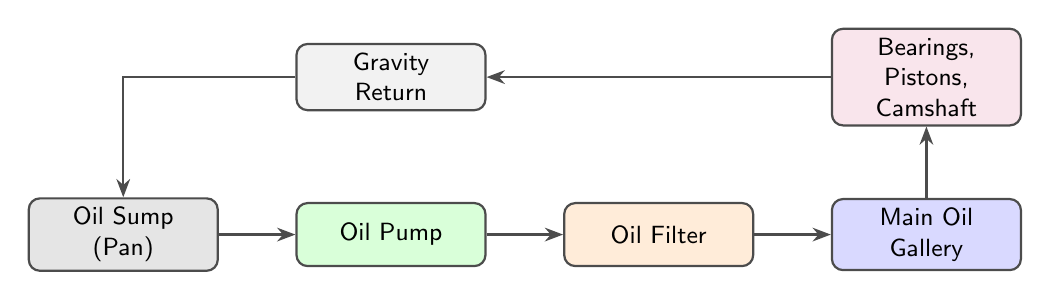
\begin{tikzpicture}[
  box/.style={draw=black!70, thick, rounded corners=4pt, minimum width=2.4cm,
              minimum height=0.8cm, align=center, font=\small\sffamily},
  arr/.style={-Stealth, thick, draw=black!70}
]
  % Nodes
  \node[box, fill=gray!20]   (sump)    at (0,0) {Oil Sump\\(Pan)};
  \node[box, fill=green!15]  (pump)    at (3.4,0) {Oil Pump};
  \node[box, fill=orange!15] (filter)  at (6.8,0) {Oil Filter};
  \node[box, fill=blue!15]   (gallery) at (10.2,0) {Main Oil\\Gallery};
  \node[box, fill=purple!10] (parts)   at (10.2,2) {Bearings,\\Pistons,\\Camshaft};
  \node[box, fill=gray!10]   (return)  at (3.4,2) {Gravity\\Return};

  % Paths
  \draw[arr] (sump) -- (pump);
  \draw[arr] (pump) -- (filter);
  \draw[arr] (filter) -- (gallery);
  \draw[arr] (gallery) -- (parts);
  \draw[arr] (parts) -- (return);
  \draw[arr] (return) -| (sump);
\end{tikzpicture}
\end{center}

\vspace{0.5em}
\textbf{Part (a)(ii): Cooling Sub-System (Water-cooled)}

\vspace{0.5em}
\begin{center}
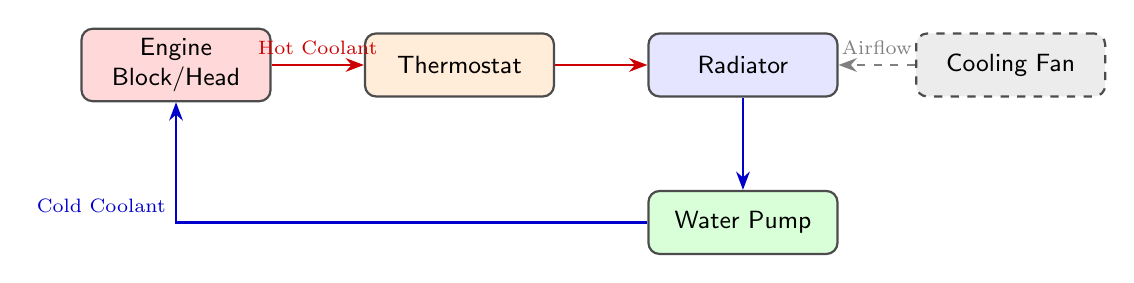
\begin{tikzpicture}[
  box/.style={draw=black!70, thick, rounded corners=4pt, minimum width=2.4cm,
              minimum height=0.8cm, align=center, font=\small\sffamily},
  arr/.style={-Stealth, thick}
]
  % Nodes
  \node[box, fill=red!15]    (eng)   at (0,0) {Engine\\Block/Head};
  \node[box, fill=orange!15] (therm) at (3.6,0) {Thermostat};
  \node[box, fill=blue!10]   (rad)   at (7.2,0) {Radiator};
  \node[box, fill=green!15]  (pump)  at (7.2,-2) {Water Pump};
  \node[box, fill=gray!15, dashed] (fan) at (10.6,0) {Cooling Fan};

  % Paths
  \draw[arr, red!80!black] (eng) -- node[above, font=\scriptsize] {Hot Coolant} (therm);
  \draw[arr, red!80!black] (therm) -- (rad);
  \draw[arr, blue!80!black] (rad) -- (pump);
  \draw[arr, blue!80!black] (pump) -| node[above left, font=\scriptsize] {Cold Coolant} (eng);
  \draw[-Stealth, dashed, thick, gray] (fan) -- node[above, font=\scriptsize] {Airflow} (rad);
\end{tikzpicture}
\end{center}

\hrulefill

\textbf{Part (b): Four-Stroke SI Cycle — P-v and T-s Diagrams}

The SI engine follows the \textbf{ideal Otto cycle}. Below are the mathematically plotted indicator and temperature-entropy diagrams:

\vspace{1em}
\begin{center}
% ===================== P-v DIAGRAM =====================
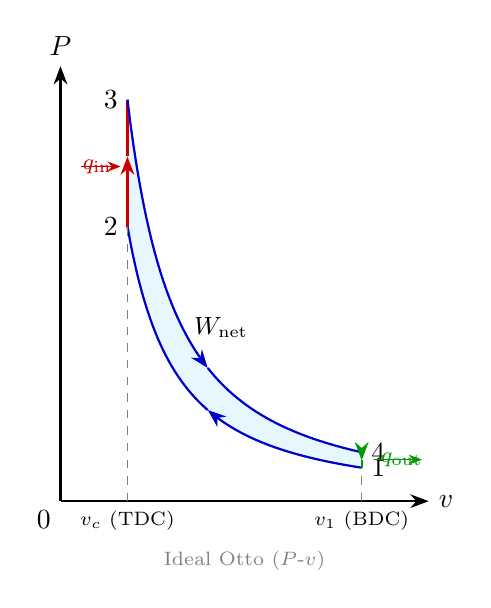
\begin{tikzpicture}[scale=0.85, arr/.style={-Stealth, thick}]
  % Axes
  \draw[arr] (0,0) -- (5.5,0) node[right] {$v$};
  \draw[arr] (0,0) -- (0,6.5) node[above] {$P$};
  \node[below left] at (0,0) {$0$};

  % Fill Area (Net Work)
  \fill[cyan!10]
    (1.0, 4.10) -- (1.0, 6.0) % 2 to 3
    -- plot[domain=1.0:4.5] (\x, {6.0*(1.0/\x)^1.4}) % 3 to 4
    -- (4.5, 0.73) % 4 to 1
    -- plot[domain=4.5:1.0] (\x, {0.5*(4.5/\x)^1.4}) % 1 to 2
    -- cycle;

  % Path 1 -> 2 (Isentropic Compression)
  \draw[-Stealth, thick, blue!80!black] plot[domain=4.5:2.2, samples=30] (\x, {0.5*(4.5/\x)^1.4});
  \draw[thick, blue!80!black] plot[domain=2.2:1.0, samples=30] (\x, {0.5*(4.5/\x)^1.4});

  % Path 2 -> 3 (Constant Volume Heat Addition)
  \draw[-Stealth, thick, red!80!black] (1.0, 4.10) -- (1.0, 5.15);
  \draw[thick, red!80!black] (1.0, 5.15) -- (1.0, 6.0);

  % Path 3 -> 4 (Isentropic Expansion)
  \draw[-Stealth, thick, blue!80!black] plot[domain=1.0:2.2, samples=30] (\x, {6.0*(1.0/\x)^1.4});
  \draw[thick, blue!80!black] plot[domain=2.2:4.5, samples=30] (\x, {6.0*(1.0/\x)^1.4});

  % Path 4 -> 1 (Constant Volume Heat Rejection)
  \draw[-Stealth, thick, green!60!black] (4.5, 0.73) -- (4.5, 0.61);
  \draw[thick, green!60!black] (4.5, 0.61) -- (4.5, 0.5);

  % Annotations & Labels
  \node[right] at (4.5, 0.5) {1};
  \node[left]  at (1.0, 4.10) {2};
  \node[left]  at (1.0, 6.0) {3};
  \node[right] at (4.5, 0.73) {4};

  \node[font=\small] at (2.4, 2.6) {$W_{\text{net}}$};
  
  \node[font=\footnotesize, red!80!black] at (0.55, 5.0) {$q_{\text{in}}$};
  \draw[-Stealth, red!80!black] (0.3, 5.0) -- (0.9, 5.0);

  \node[font=\footnotesize, green!60!black] at (5.1, 0.62) {$q_{\text{out}}$};
  \draw[-Stealth, green!60!black] (4.7, 0.62) -- (5.4, 0.62);

  \draw[dashed, gray] (1.0, 0) -- (1.0, 4.10);
  \draw[dashed, gray] (4.5, 0) -- (4.5, 0.5);
  \node[below, font=\scriptsize] at (1.0, 0) {$v_c$ (TDC)};
  \node[below, font=\scriptsize] at (4.5, 0) {$v_1$ (BDC)};
  \node[below, font=\scriptsize, text=gray] at (2.75, -0.6) {Ideal Otto ($P$-$v$)};
\end{tikzpicture}
\hfill
% ===================== T-s DIAGRAM =====================
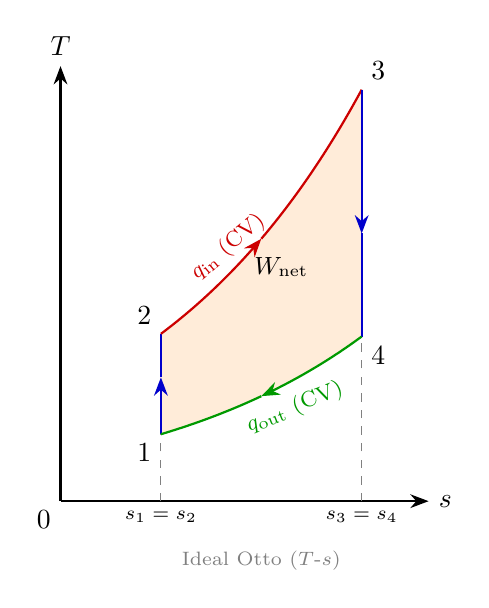
\begin{tikzpicture}[scale=0.85, arr/.style={-Stealth, thick}]
  % Axes
  \draw[arr] (0,0) -- (5.5,0) node[right] {$s$};
  \draw[arr] (0,0) -- (0,6.5) node[above] {$T$};
  \node[below left] at (0,0) {$0$};

  % Fill Area (Net Work)
  \fill[orange!15]
    (1.5, 2.5) -- plot[domain=1.5:4.5] (\x, {2.5*exp((\x-1.5)*0.3)}) % 2 to 3
    -- (4.5, 2.46) % 3 to 4
    -- plot[domain=4.5:1.5] (\x, {2.46*exp((\x-4.5)*0.3)}) % 4 to 1
    -- cycle;

  % Path 1 -> 2 (Isentropic Compression)
  \draw[-Stealth, thick, blue!80!black] (1.5, 1.0) -- (1.5, 1.85);
  \draw[thick, blue!80!black] (1.5, 1.85) -- (1.5, 2.5);

  % Path 2 -> 3 (Constant Volume Heat Addition)
  \draw[-Stealth, thick, red!80!black] plot[domain=1.5:3.0, samples=30] (\x, {2.5*exp((\x-1.5)*0.3)});
  \draw[thick, red!80!black] plot[domain=3.0:4.5, samples=30] (\x, {2.5*exp((\x-1.5)*0.3)});

  % Path 3 -> 4 (Isentropic Expansion)
  \draw[-Stealth, thick, blue!80!black] (4.5, 6.15) -- (4.5, 4.0);
  \draw[thick, blue!80!black] (4.5, 4.0) -- (4.5, 2.46);

  % Path 4 -> 1 (Constant Volume Heat Rejection)
  \draw[-Stealth, thick, green!60!black] plot[domain=4.5:3.0, samples=30] (\x, {2.46*exp((\x-4.5)*0.3)});
  \draw[thick, green!60!black] plot[domain=3.0:1.5, samples=30] (\x, {2.46*exp((\x-4.5)*0.3)});

  % Annotations & Labels
  \node[below left] at (1.5, 1.0) {1};
  \node[above left] at (1.5, 2.5) {2};
  \node[above right] at (4.5, 6.15) {3};
  \node[below right] at (4.5, 2.46) {4};

  \node[font=\small] at (3.3, 3.5) {$W_{\text{net}}$};

  \node[font=\footnotesize, red!80!black, rotate=40] at (2.5, 3.8) {$q_{\text{in}}$ (CV)};
  \node[font=\footnotesize, green!60!black, rotate=22] at (3.5, 1.4) {$q_{\text{out}}$ (CV)};

  \draw[dashed, gray] (1.5, 0) -- (1.5, 1.0);
  \draw[dashed, gray] (4.5, 0) -- (4.5, 2.46);
  \node[below, font=\scriptsize] at (1.5, 0) {$s_1 = s_2$};
  \node[below, font=\scriptsize] at (4.5, 0) {$s_3 = s_4$};
  \node[below, font=\scriptsize, text=gray] at (3.0, -0.6) {Ideal Otto ($T$-$s$)};
\end{tikzpicture}
\end{center}

\textbf{Process summary:}
\begin{itemize}[label={--}, noitemsep, topsep=2pt, leftmargin=2em]
  \item $1\to2$: Reversible adiabatic (isentropic) compression.
  \item $2\to3$: Constant-volume heat addition.
  \item $3\to4$: Reversible adiabatic (isentropic) expansion.
  \item $4\to1$: Constant-volume heat rejection.
\end{itemize}

\hrulefill

\textbf{Part (c): Valve Timing — Ideal vs.\ Actual Engine}

\textbf{Ideal engine:} Valves open and close exactly at TDC and BDC;
no valve overlap; instantaneous transitions.

\begin{center}
  
\includegraphics[height=0.3\textheight,width=0.75\textwidth,keepaspectratio]{/idealvalve.png}
\end{center}

\textbf{Actual (medium-performance) engine:}
IVO 10--20\textdegree\ bTDC;\; IVC 30--60\textdegree\ aBDC;\;
EVO 25--55\textdegree\ bBDC;\; EVC 10--30\textdegree\ aTDC;\;
Valve overlap $\approx$20--50\textdegree.

\begin{center}
  
\includegraphics[height=0.3\textheight,width=0.75\textwidth,keepaspectratio]{/A21.png}
\end{center}

\end{tcolorbox}
%%────────────────────────────────────────────────────────────
%% A2-Q20
%%────────────────────────────────────────────────────────────
\item \label{qlabel:A2-Q17}
(a) With necessary sketches, briefly describe the working principle of a four-stroke IC engine. \mk{18}\\
(b) A four-stroke IC engine: bore\,$\times$\,stroke\,$= 10$\,cm\,$\times$\,10\,cm, clearance volume\,$= 100\pi$\,cc. Find: (i) total volume per cylinder, (ii) compression ratio, (iii) whether SI or CI, (iv) engine displacement for 4 cylinders. \mk{12}\\
(c) Draw the actual and ideal thermodynamic cycle of a petrol engine. \mk{5}
\yr{2011--12}

\begin{tcolorbox}[enhanced,breakable,ansbox,colback=cB!4,colframe=cB,
  boxrule=0.8pt,arc=5pt,
  title={\textbf{Answer}},fonttitle=\bfseries\color{white},colbacktitle=cB]

\textbf{Part (a):} Four-stroke IC engine operation — \variant{A2-Q6 — identical; full answer with sketch given there}

\hrulefill

\textbf{Part (b): Numerical Solution}

\textbf{Given:} $d = 10$\,cm, $L = 10$\,cm, $V_c = 100\pi\,\text{cm}^3$.

\textbf{(i) Swept volume per cylinder:}
\[
  V_s = \frac{\pi}{4}d^2 L = \frac{\pi}{4}\times100\times10 = 250\pi\,\text{cm}^3 \approx 785.40\,\text{cm}^3
\]

\textbf{Total volume per cylinder:}
\[
  V_{\text{total}} = V_s + V_c = 250\pi + 100\pi = \boxed{350\pi \approx 1099.56\,\text{cm}^3}
\]

\textbf{(ii) Compression ratio:}
\[
  r = \frac{V_s + V_c}{V_c} = \frac{350\pi}{100\pi} = \boxed{3.5}
\]

\textbf{(iii) SI or CI?}

A compression ratio of $r = 3.5$ is far too low for either SI (which requires
$r \geq 6$) or CI engines ($r \geq 15$). With such a low ratio, temperature rise
at end of compression would be insufficient for combustion. In practice this
would be classified as an \textbf{SI engine} (petrol), as CI requires much higher
$r$. \textit{Note: the problem values appear theoretical/pedagogical.}

\textbf{(iv) Engine displacement for 4 cylinders:}
\[
  V_{\text{engine}} = 4\times V_s = 4\times250\pi
  = 1000\pi \approx \boxed{3141.59\,\text{cm}^3 \approx 3.14\,\text{L}}
\]

\hrulefill

\textbf{Part (c): Ideal vs.\ Actual Otto (Petrol) Cycle}


\begin{center}
  
\includegraphics[height=0.3\textheight,width=0.75\textwidth,keepaspectratio]{/actualPetrolcycle.png}
\end{center}

\begin{center}
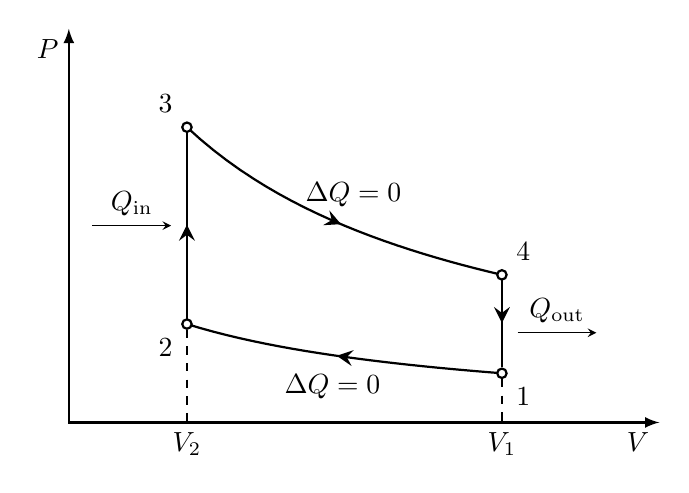
\begin{tikzpicture}
    % P-V Axis
    \draw[latex-latex, thick] (-0.5,5) node[below left]{$P$} |- (7,0) node[below left]{$V$};
    
    % Otto Cycle
    \begin{scope}[thick]
    \draw[annotate={label=below right:1,alias=1}{$\Delta Q=0$}] plot[variable=\x,domain=5:1] (\x,{5/(\x+3)});
    \draw[annotate={label=above left:3,alias=3}{$\Delta Q=0$}] plot[variable=\x,domain=1:5] (\x,{15/(\x+3)});
    \draw[annotate={label=below left:2,alias=2}{}] (1,5/4) -- (3);
    \draw[annotate={label=above right:4,alias=4}{}] (5,15/8) -- (1);  
    \end{scope} 
    
    \path (2) -- (3) coordinate[pos=0.5] (23) (1) -- (4) coordinate[pos=0.4] (14);
    
    % Q_in and Q_out
    \draw[stealth-] ([xshift=-2mm, thick]23) -- ++ (-1,0) node[midway,above]{$Q_\text{in}$};
    \draw[-stealth] ([xshift=2mm, thick]14) -- ++ (1,0) node[midway,above]{$Q_\text{out}$};
    
    % Dashed Lines    
    \draw[dashed, thick] (1) -- (1|-0,0) node[below] {$V_1$};
    \draw[dashed, thick] (2) -- (2|-0,0) node[below] {$V_2$};    
\end{tikzpicture}
\end{center}


Key differences: actual cycle has \emph{rounded corners} (finite combustion
duration), \emph{lower peak pressure} (heat losses, incomplete combustion),
\emph{valve throttling losses} on intake/exhaust, and \emph{blowdown} before BDC.

\end{tcolorbox}

%%────────────────────────────────────────────────────────────
%% A2-Q18
%%────────────────────────────────────────────────────────────
\item \label{qlabel:A2-Q18}
(a) With necessary sketches, describe the operating principle of a closed-loop gas turbine. Draw the corresponding thermodynamic cycle. \mk{18}\\
(b) With T-S diagrams, explain the merits of adding regeneration, inter-cooling and reheating to a closed-loop gas turbine. \mk{17}
\yr{2011--12}

\begin{tcolorbox}[enhanced,breakable,ansbox,colback=cB!4,colframe=cB,
  boxrule=0.8pt,arc=5pt,
  title={\textbf{Answer}},fonttitle=\bfseries\color{white},colbacktitle=cB]

\textbf{Part (a): Closed-Loop Gas Turbine}

In a \textbf{closed-loop (closed-cycle) gas turbine}, the working fluid
circulates continuously in a closed loop and never contacts the combustion
products directly. Heat is added via an external heat exchanger.

\textbf{Brayton Cycle Processes:}
\begin{itemize}[leftmargin=1.5em,itemsep=2pt]
  \item $1\to2$: \textbf{Isentropic compression} in compressor.
  \item $2\to3$: \textbf{Constant-pressure heat addition} in heat exchanger
        (from external source — nuclear, solar, or combustion gases).
  \item $3\to4$: \textbf{Isentropic expansion} in turbine (produces work output).
  \item $4\to1$: \textbf{Constant-pressure heat rejection} in cooler.
\end{itemize}

\vspace{1em}
\begin{center}
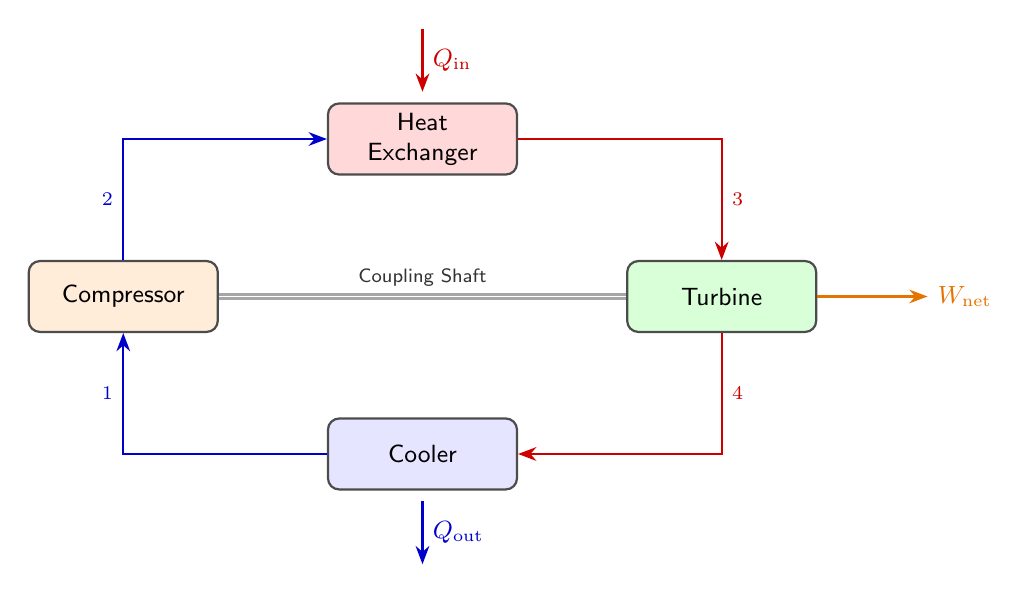
\begin{tikzpicture}[
  box/.style={draw=black!70, thick, rounded corners=4pt, minimum width=2.4cm,
              minimum height=0.9cm, align=center, font=\small\sffamily},
  arr/.style={-Stealth, thick, draw=black!80}
]
  % Nodes
  \node[box, fill=orange!15] (comp) at (0,0)  {Compressor};
  \node[box, fill=red!15]    (hx)   at (3.8,2) {Heat\\Exchanger};
  \node[box, fill=green!15]  (turb) at (7.6,0)  {Turbine};
  \node[box, fill=blue!10]   (cool) at (3.8,-2) {Cooler};

  % Shaft connecting compressor and turbine
  \draw[thick, double, draw=gray!70] (comp.east) -- (turb.west) 
    node[midway, above, font=\scriptsize\sffamily, text=black!80] {Coupling Shaft};

  % Piping Paths
  \draw[arr, blue!80!black] (comp.north) |- node[near start, left, font=\scriptsize] {2} (hx.west);
  \draw[arr, red!80!black]  (hx.east) -| node[near end, right, font=\scriptsize] {3} (turb.north);
  \draw[arr, red!80!black]  (turb.south) |- node[near start, right, font=\scriptsize] {4} (cool.east);
  \draw[arr, blue!80!black] (cool.west) -| node[near end, left, font=\scriptsize] {1} (comp.south);

  % Heat Input/Output & Work Arrows
  \draw[-Stealth, thick, red!80!black] (3.8, 3.4) -- (3.8, 2.6) 
    node[midway, right, font=\small] {$Q_{\text{in}}$};
  \draw[-Stealth, thick, blue!80!black] (3.8, -2.6) -- (3.8, -3.4) 
    node[midway, right, font=\small] {$Q_{\text{out}}$};
  \draw[-Stealth, thick, orange!90!black] (turb.east) -- ++(1.4,0) 
    node[right, font=\small] {$W_{\text{net}}$};
\end{tikzpicture}
\end{center}

\vspace{1em}
\textbf{P-v and T-s diagrams of the ideal Brayton cycle:}

\vspace{0.5em}
\begin{center}
% ===================== P-v DIAGRAM =====================
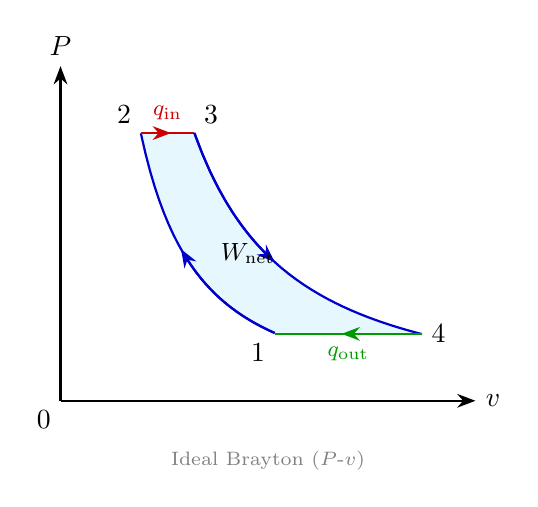
\begin{tikzpicture}[scale=0.85, arr/.style={-Stealth, thick}]
  \draw[arr] (0,0) -- (6.2,0) node[right] {$v$};
  \draw[arr] (0,0) -- (0,5.0) node[above] {$P$};
  \node[below left] at (0,0) {$0$};

  % Fill Area (Net Work)
  \fill[cyan!10]
    (3.2, 1.0) -- plot[domain=3.2:1.2] (\x, {5.16/(\x^1.4)}) % 1 to 2
    -- (2.0, 4.0) % 2 to 3
    -- plot[domain=2.0:5.4] (\x, {10.56/(\x^1.4)}) % 3 to 4
    -- cycle; % 4 to 1

  % Path 1 -> 2 (Isentropic Compression)
  \draw[thick, blue!80!black] plot[domain=3.2:1.2, samples=30] (\x, {5.16/(\x^1.4)});
  \draw[-Stealth, thick, blue!80!black] plot[domain=3.2:1.8, samples=20] (\x, {5.16/(\x^1.4)});

  % Path 2 -> 3 (Isobaric Heat Addition)
  \draw[thick, red!80!black] (1.2, 4.0) -- (2.0, 4.0);
  \draw[-Stealth, thick, red!80!black] (1.2, 4.0) -- (1.65, 4.0);

  % Path 3 -> 4 (Isentropic Expansion)
  \draw[thick, blue!80!black] plot[domain=2.0:5.4, samples=30] (\x, {10.56/(\x^1.4)});
  \draw[-Stealth, thick, blue!80!black] plot[domain=2.0:3.2, samples=20] (\x, {10.56/(\x^1.4)});

  % Path 4 -> 1 (Isobaric Heat Rejection)
  \draw[thick, green!60!black] (5.4, 1.0) -- (3.2, 1.0);
  \draw[-Stealth, thick, green!60!black] (5.4, 1.0) -- (4.2, 1.0);

  % Annotations & Labels
  \node[above left]  at (1.2, 4.0) {2};
  \node[above right] at (2.0, 4.0) {3};
  \node[right]       at (5.4, 1.0) {4};
  \node[below left]  at (3.2, 1.0) {1};

  \node[font=\small] at (2.8, 2.2) {$W_{\text{net}}$};
  
  \node[font=\footnotesize, red!80!black] at (1.6, 4.3) {$q_{\text{in}}$};
  \node[font=\footnotesize, green!60!black] at (4.3, 0.7) {$q_{\text{out}}$};
  
  \node[below, font=\scriptsize, text=gray] at (3.1, -0.6) {Ideal Brayton ($P$-$v$)};
\end{tikzpicture}
\hfill
% ===================== T-s DIAGRAM =====================
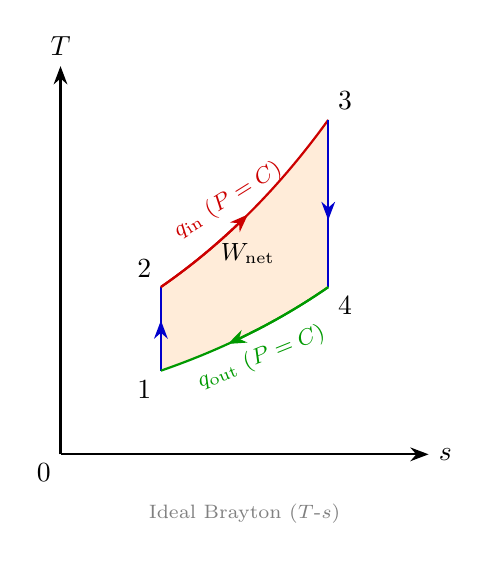
\begin{tikzpicture}[scale=0.85, arr/.style={-Stealth, thick}]
  \draw[arr] (0,0) -- (5.5,0) node[right] {$s$};
  \draw[arr] (0,0) -- (0,5.8) node[above] {$T$};
  \node[below left] at (0,0) {$0$};

  % Fill Area (Net Work)
  \fill[orange!15]
    (1.5, 1.25) -- (1.5, 2.5) % 1 to 2
    -- plot[domain=1.5:4.0] (\x, {2.5*exp(0.277*(\x-1.5))}) % 2 to 3
    -- (4.0, 2.5) % 3 to 4
    -- plot[domain=4.0:1.5] (\x, {1.25*exp(0.277*(\x-1.5))}) % 4 to 1
    -- cycle;

  % Path 1 -> 2 (Isentropic)
  \draw[thick, blue!80!black] (1.5, 1.25) -- (1.5, 2.5);
  \draw[-Stealth, thick, blue!80!black] (1.5, 1.25) -- (1.5, 2.0);

  % Path 2 -> 3 (Isobaric)
  \draw[thick, red!80!black] plot[domain=1.5:4.0, samples=30] (\x, {2.5*exp(0.277*(\x-1.5))});
  \draw[-Stealth, thick, red!80!black] plot[domain=1.5:2.8, samples=20] (\x, {2.5*exp(0.277*(\x-1.5))});

  % Path 3 -> 4 (Isentropic)
  \draw[thick, blue!80!black] (4.0, 5.0) -- (4.0, 2.5);
  \draw[-Stealth, thick, blue!80!black] (4.0, 5.0) -- (4.0, 3.5);

  % Path 4 -> 1 (Isobaric)
  \draw[thick, green!60!black] plot[domain=4.0:1.5, samples=30] (\x, {1.25*exp(0.277*(\x-1.5))});
  \draw[-Stealth, thick, green!60!black] plot[domain=4.0:2.5, samples=20] (\x, {1.25*exp(0.277*(\x-1.5))});

  % Annotations & Labels
  \node[below left]  at (1.5, 1.25) {1};
  \node[above left]  at (1.5, 2.5) {2};
  \node[above right] at (4.0, 5.0) {3};
  \node[below right] at (4.0, 2.5) {4};

  \node[font=\small] at (2.8, 3.0) {$W_{\text{net}}$};
  
  \node[font=\footnotesize, red!80!black, rotate=32] at (2.5, 3.8) {$q_{\text{in}}$ ($P=C$)};
  \node[font=\footnotesize, green!60!black, rotate=22] at (3.0, 1.45) {$q_{\text{out}}$ ($P=C$)};
  
  \node[below, font=\scriptsize, text=gray] at (2.75, -0.6) {Ideal Brayton ($T$-$s$)};
\end{tikzpicture}
\end{center}

\hrulefill

\textbf{Part (b): Regeneration, Inter-cooling, and Reheating}

\begin{itemize}[leftmargin=1.5em,itemsep=5pt]
  \item \textbf{Regeneration:} A regenerator (heat exchanger) transfers heat
        from the hot turbine exhaust (state 4) to the compressed air before
        the heat exchanger (state 2). This reduces external heat input required
        and improves thermal efficiency. On the T-s diagram, the area
        representing $Q_{\text{in}}$ shrinks while the net work remains the
        same.
  \item \textbf{Inter-cooling:} Compression is performed in two stages with
        cooling between stages. Cooling the gas before the second compressor
        stage reduces the compression work (since work $\propto T$). The T-s
        diagram shows the compression path shifted left, reducing the work
        input area.
  \item \textbf{Reheating:} Expansion is performed in two turbine stages with
        reheating between them. Adding heat between expansion stages increases
        turbine work output. The T-s diagram shows an additional heat
        addition loop at the turbine exit, increasing the work output area.
\end{itemize}

\textbf{Combined effect:} All three modifications together substantially increase
the thermal efficiency and specific work output. Their T-s diagram shows a more
rectangular cycle, approaching the Carnot efficiency.

\end{tcolorbox}

%%────────────────────────────────────────────────────────────
%% A2-Q19
%%────────────────────────────────────────────────────────────
\item \label{qlabel:A2-Q15}
(a) Give a simplistic definition of an Internal Combustion Engine. \mk{6}\\
(b) Classify engines on the basis of combustion method. \mk{8}\\
(c) Give a brief comparison between spark ignition and compression ignition engines. \mk{9}
\yr{2010--11}

\begin{tcolorbox}[enhanced,breakable,ansbox,colback=cB!4,colframe=cB,
  boxrule=0.8pt,arc=5pt,
  title={\textbf{Answer}},fonttitle=\bfseries\color{white},colbacktitle=cB]

\textbf{Part (a): Definition of an IC Engine}

An \textbf{Internal Combustion (IC) Engine} is a device in which the chemical
energy of a fuel is released by burning it \emph{inside the engine cylinder}
itself, and the resulting high-pressure combustion gases act directly on a piston
(or rotor) to produce useful mechanical work.

\hrulefill

\textbf{Part (b): Classification by Combustion Method}

\begin{itemize}[leftmargin=1.5em,itemsep=3pt]
  \item \textbf{Spark Ignition (SI) Engine:} A high-voltage spark from a spark
        plug ignites a pre-mixed homogeneous air--fuel charge. Used with
        high-volatility fuels such as petrol/gasoline. Compression ratio
        $r = 6$--12.
  \item \textbf{Compression Ignition (CI) Engine:} Air alone is compressed to
        very high temperature ($\approx$550\textdegree C); fuel is then injected
        and auto-ignites without any external ignition source. Used with diesel
        fuel. Compression ratio $r = 15$--25.
  \item \textbf{Homogeneous Charge Compression Ignition (HCCI):} A modern
        variant in which a premixed charge auto-ignites simultaneously
        throughout the cylinder due to high compression, combining benefits of
        both SI and CI engines (high efficiency and low emissions).
\end{itemize}

\hrulefill

\textbf{Part (c): SI vs.\ CI Engine Comparison}

\begin{center}
\small
\begin{tabular}{@{}llll@{}}
\toprule
\textbf{No.} & \textbf{Feature}        & \textbf{SI Engine}         & \textbf{CI Engine} \\
\midrule
i   & Ignition source          & Electric spark plug         & Self-ignition (compression) \\
ii  & Fuel                     & Petrol/Gasoline             & Diesel \\
iii & Air--fuel supply         & Carburettor/port injection  & Direct high-pressure injection \\
iv  & Compression ratio        & 6--12                       & 15--25 \\
v   & Thermal efficiency       & $\approx$25--30\%           & $\approx$35--45\% \\
vi  & Engine weight/size       & Lighter, cheaper            & Heavier, costlier \\
vii & Speed                    & Higher RPM                  & Lower RPM \\
viii& Maintenance              & Easier, cheaper             & More expensive \\
ix  & Applications             & Cars, motorcycles           & Trucks, buses, ships \\
x   & Compression pressure     & $\approx$10\,bar at end     & $\approx$35\,bar at end \\
\bottomrule
\end{tabular}
\end{center}

\end{tcolorbox}

%%────────────────────────────────────────────────────────────
%% A2-Q16
%%────────────────────────────────────────────────────────────
\item \label{qlabel:A2-Q16}
Draw the fuel supply system layout of a compression ignition engine with individual fuel pumps for each cylinder. \mk{12}
\yr{2010--11}

\begin{tcolorbox}[enhanced,breakable,ansbox,colback=cB!4,colframe=cB,
  boxrule=0.8pt,arc=5pt,
  title={\textbf{Answer}},fonttitle=\bfseries\color{white},colbacktitle=cB]

\textbf{Fuel Supply System — CI Engine (Individual Pump per Cylinder):}

\begin{center}
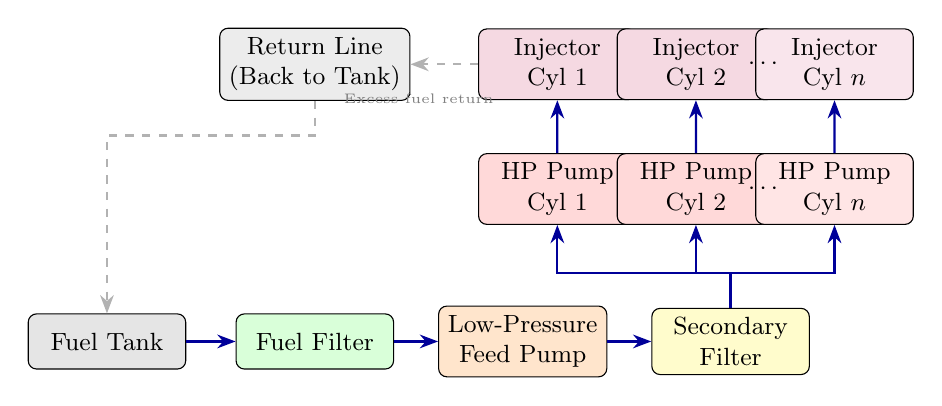
\begin{tikzpicture}[scale=0.88,
  box/.style={draw,rounded corners=3pt,fill=blue!10,minimum width=2.0cm,
              minimum height=0.7cm,align=center,font=\small},
  arr/.style={-Stealth,thick,blue!60!black}]

  \node[box,fill=gray!20]  (tank)   at (0,0)    {Fuel Tank};
  \node[box,fill=green!15] (filter) at (3,0)    {Fuel Filter};
  \node[box,fill=orange!20](lp)     at (6,0)    {Low-Pressure\\Feed Pump};
  \node[box,fill=yellow!20](sec)    at (9,0)    {Secondary\\Filter};
  \node[box,fill=red!15]   (pump1)  at (6.5,2.2){HP Pump\\Cyl 1};
  \node[box,fill=red!15]   (pump2)  at (8.5,2.2){HP Pump\\Cyl 2};
  \node[box,fill=red!10]   (pumpn)  at (10.5,2.2){HP Pump\\Cyl $n$};
  \node[box,fill=purple!15](inj1)   at (6.5,4.0) {Injector\\Cyl 1};
  \node[box,fill=purple!15](inj2)   at (8.5,4.0) {Injector\\Cyl 2};
  \node[box,fill=purple!10](injn)   at (10.5,4.0){Injector\\Cyl $n$};
  \node[box,fill=gray!15]  (ret)    at (3,4.0)   {Return Line\\(Back to Tank)};

  \draw[arr] (tank)--(filter);
  \draw[arr] (filter)--(lp);
  \draw[arr] (lp)--(sec);
  \draw[arr] (sec.north) -- ++(0,0.5) -| (pump1.south);
  \draw[arr] (sec.north) -- ++(0,0.5) -| (pump2.south);
  \draw[arr] (sec.north) -- ++(0,0.5) -| (pumpn.south);
  \draw[arr] (pump1)--(inj1);
  \draw[arr] (pump2)--(inj2);
  \draw[arr] (pumpn)--(injn);
  \draw[arr,dashed,gray!60] (inj1.west) -- ++(-0.5,0) |- (ret.east);
  \draw[arr,dashed,gray!60] (ret.south) -- ++(0,-0.5) -| (tank.north);
  \node[font=\tiny,gray] at (4.5,3.5) {Excess fuel return};
  \node[font=\small] at (9.5,2.2) {$\cdots$};
  \node[font=\small] at (9.5,4.0) {$\cdots$};

\end{tikzpicture}
\end{center}

\textbf{Component Description:}
\begin{itemize}[leftmargin=1.5em,itemsep=2pt]
  \item \textbf{Fuel Tank:} Stores diesel fuel.
  \item \textbf{Fuel Filter (Primary):} Removes large particles.
  \item \textbf{Low-Pressure Feed Pump:} Draws fuel from tank and maintains
        supply pressure to high-pressure pumps.
  \item \textbf{Secondary Filter:} Fine filtration before high-pressure stage.
  \item \textbf{Individual High-Pressure (HP) Pumps:} One per cylinder;
        pressurises fuel to injection pressure ($\approx$150--200\,bar).
  \item \textbf{Fuel Injectors:} Atomise and inject fuel directly into cylinder
        at precise timing and quantity.
  \item \textbf{Return Line:} Excess fuel from injectors returned to tank to
        maintain fuel circulation and cooling.
\end{itemize}

\end{tcolorbox}

%%────────────────────────────────────────────────────────────
%% A2-Q17
%%────────────────────────────────────────────────────────────
\item \label{qlabel:A2-Q23}
(a) Explain the importance of engine cooling. \mk{9}\\
(b) Draw a neat sketch of a water cooling system for an IC engine. \mk{10}\\
(c) Describe the fuel supply system of a spark ignition engine with neat sketch. \mk{16}
\yr{2008--09}

\begin{tcolorbox}[enhanced,breakable,ansbox,colback=cB!4,colframe=cB,
  boxrule=0.8pt,arc=5pt,
  title={\textbf{Answer}},fonttitle=\bfseries\color{white},colbacktitle=cB]

\textbf{Part (a): Importance of Engine Cooling}

Combustion temperatures in an IC engine can reach 2000--2500\textdegree C.
Without cooling:
\begin{itemize}[leftmargin=1.5em,itemsep=2pt]
  \item \textbf{Mechanical failure:} Pistons, valves and cylinder walls would
        melt or seize.
  \item \textbf{Lubricant breakdown:} Engine oil loses viscosity at high
        temperatures, increasing wear.
  \item \textbf{Knocking:} Excessive heat causes pre-ignition/detonation in SI
        engines.
  \item \textbf{Reduced volumetric efficiency:} Hot cylinder walls heat the
        incoming charge, reducing its density and thus power output.
  \item \textbf{Thermal stresses:} Temperature gradients cause distortion and
        cracking of engine components.
\end{itemize}
Cooling removes about 30\% of the total heat generated, maintaining metal
temperatures within safe operating limits ($\approx$200--250\textdegree C for
aluminium pistons).

\hrulefill

\textbf{Part (b): Water Cooling System}

\begin{center}
  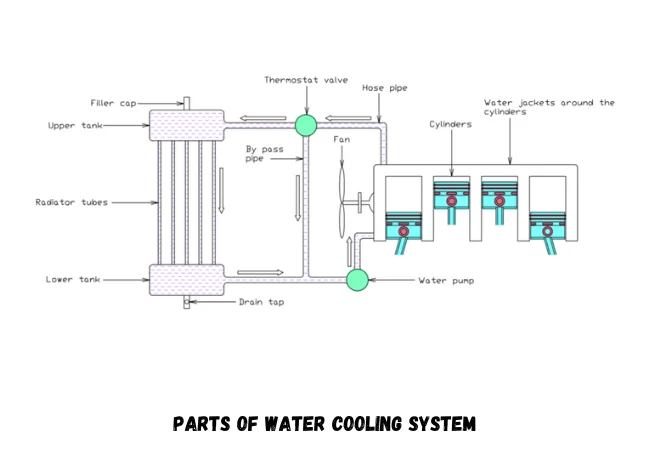
\includegraphics{Parts-of-Water-Cooling-System.png}
\end{center}

\textbf{Components:}
Water pump circulates coolant; thermostat regulates temperature (bypasses
radiator when cold); radiator dissipates heat to air; fan enhances airflow through
radiator; expansion tank accommodates coolant volume changes with temperature.

\hrulefill

\textbf{Part (c): Fuel Supply System — SI Engine}

\begin{center}
  
\includegraphics[width=0.75\textwidth,keepaspectratio]{/fuel.png}
\end{center}
\textbf{Description:}
\begin{itemize}[leftmargin=1.5em,itemsep=2pt]
  \item \textbf{Fuel tank:} Stores petrol; fitted with fuel level sensor.
  \item \textbf{Fuel pump (electric):} Maintains supply pressure
        ($\approx$3--4\,bar for port injection).
  \item \textbf{Fuel filter:} Removes contaminants to protect injectors.
  \item \textbf{Fuel rail:} Distributes fuel at constant pressure to all
        injectors.
  \item \textbf{Pressure regulator:} Maintains constant differential pressure
        across injectors; excess fuel returned to tank.
  \item \textbf{Fuel injectors:} Electronically controlled solenoid valves that
        spray a precise quantity of atomised fuel into the intake port (port
        injection) or directly into the cylinder (direct injection), timed with
        the intake stroke.
\end{itemize}

\end{tcolorbox}

%%────────────────────────────────────────────────────────────
%% A2-Q24
%%────────────────────────────────────────────────────────────
\item \label{qlabel:A2-Q24}
(a) Draw a neat sketch of the spark ignition system for a four-cylinder engine. \mk{9}\\
(b) Describe the actual valve timing diagram of a four-stroke SI engine. \mk{14}\\
(c) Describe the Otto cycle and Dual cycle on p-v and T-s planes. \mk{12}
\yr{2008--09}

\begin{tcolorbox}[enhanced,breakable,ansbox,colback=cB!4,colframe=cB,
  boxrule=0.8pt,arc=5pt,
  title={\textbf{Answer}},fonttitle=\bfseries\color{white},colbacktitle=cB]

\textbf{Part (a): Spark Ignition System — 4-Cylinder Engine}


\begin{center}
  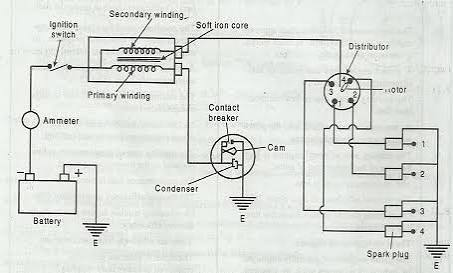
\includegraphics[height=0.3\textheight,width=0.75\textwidth,keepaspectratio]{images/sparkIgnitionSystem.jpeg}
\end{center}

The ignition coil steps up 12\,V to $\sim$20--24\,kV. The distributor
sequentially directs this high voltage to each spark plug in the firing order
(1-3-4-2 for inline 4-cylinder), timed with the compression stroke of each
cylinder.

\hrulefill

\textbf{Part (b): Actual Valve Timing Diagram}

\variant{A2-Q7(b) — full diagram and explanation given there}

Key timings:
\begin{itemize}[leftmargin=1.5em,itemsep=1pt]
  \item \textbf{IVO} 10--20\textdegree\ bTDC: allows full opening by TDC.
  \item \textbf{IVC} 30--60\textdegree\ aBDC: exploits ram effect.
  \item \textbf{EVO} 25--55\textdegree\ bBDC: blowdown reduces exhaust work.
  \item \textbf{EVC} 10--30\textdegree\ aTDC: kinetic energy assists scavenging.
  \item \textbf{Ignition} 20--30\textdegree\ bTDC: spark advance.
  \item \textbf{Valve overlap} $\approx$ 20--50\textdegree.
\end{itemize}

\hrulefill

\textbf{Part (c): Otto Cycle and Dual Cycle}

\textbf{Otto Cycle:}
All heat is added at \emph{constant volume} (processes $2\to3$).
\variant{A2-Q19(b) — P-v and T-s diagrams given there}

\textbf{Dual (Mixed/Semi-Diesel) Cycle:} Combines features of Otto and Diesel
— part of heat is added at \emph{constant volume} and the remainder at
\emph{constant pressure}.

\begin{center}
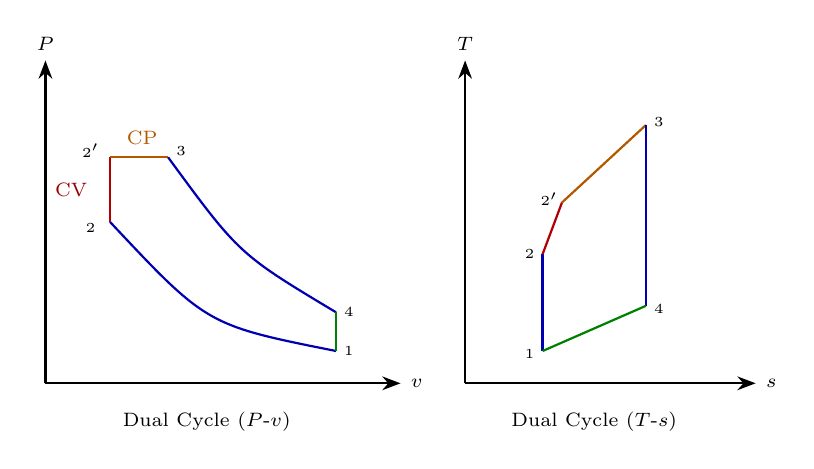
\begin{tikzpicture}[scale=0.82,arr/.style={-Stealth,thick}]
  %% Dual cycle P-v
  \begin{scope}[xshift=0cm]
    \draw[arr](0,0)--(5.5,0) node[right,font=\scriptsize]{$v$};
    \draw[arr](0,0)--(0,5.0) node[above,font=\scriptsize]{$P$};
    % 1->2 isentropic
    \draw[thick,blue!70!black]
      (4.5,0.5) .. controls (2.5,0.9) .. (1.0,2.5);
    % 2->2' const V heat add
    \draw[thick,red!70!black] (1.0,2.5)--(1.0,3.5);
    % 2'->3 const P heat add
    \draw[thick,orange!70!black] (1.0,3.5)--(1.9,3.5);
    % 3->4 isentropic expansion
    \draw[thick,blue!70!black]
      (1.9,3.5) .. controls (3.0,2.0) .. (4.5,1.1);
    % 4->1 const V heat rej
    \draw[thick,green!50!black] (4.5,1.1)--(4.5,0.5);
    \node[font=\tiny] at (4.7,0.5)  {1};
    \node[font=\tiny] at (0.7,2.4)  {2};
    \node[font=\tiny] at (0.7,3.6)  {$2'$};
    \node[font=\tiny] at (2.1,3.6)  {3};
    \node[font=\tiny] at (4.7,1.1)  {4};
    \node[font=\scriptsize,red!60!black]    at (0.4,3.0) {CV};
    \node[font=\scriptsize,orange!70!black] at (1.5,3.8) {CP};
    \node[font=\scriptsize,below] at (2.5,-0.3) {Dual Cycle ($P$-$v$)};
  \end{scope}
  %% Dual cycle T-s
  \begin{scope}[xshift=6.5cm]
    \draw[arr](0,0)--(4.5,0) node[right,font=\scriptsize]{$s$};
    \draw[arr](0,0)--(0,5.0) node[above,font=\scriptsize]{$T$};
    % 1->2 isentropic (vertical)
    \draw[thick,blue!70!black] (1.2,0.5)--(1.2,2.0);
    % 2->2' const V (vertical, steeper)
    \draw[thick,red!70!black]  (1.2,2.0)--(1.5,2.8);
    % 2'->3 const P (fan-shaped)
    \draw[thick,orange!70!black](1.5,2.8)--(2.8,4.0);
    % 3->4 isentropic
    \draw[thick,blue!70!black] (2.8,4.0)--(2.8,1.2);
    % 4->1 const V
    \draw[thick,green!50!black](2.8,1.2)--(1.2,0.5);
    \node[font=\tiny] at (1.0,0.45) {1};
    \node[font=\tiny] at (1.0,2.0)  {2};
    \node[font=\tiny] at (1.3,2.85) {$2'$};
    \node[font=\tiny] at (3.0,4.05) {3};
    \node[font=\tiny] at (3.0,1.15) {4};
    \node[font=\scriptsize,below] at (2.0,-0.3) {Dual Cycle ($T$-$s$)};
  \end{scope}
\end{tikzpicture}
\end{center}

\end{tcolorbox}

%%────────────────────────────────────────────────────────────
%% A2-Q25
%%────────────────────────────────────────────────────────────
\item \label{qlabel:A2-Q25}
(a) Define an isentropic process. Which strokes of an ideal Otto cycle are isentropic? \mk{7}\\
(b) With necessary sketches, explain the coil-ignition system of a 4-stroke SI engine. \mk{13}\\
(c) Draw the actual valve timing diagram of a 4-stroke diesel engine showing all valve openings and closings. \mk{8}\\
(d) What do you understand by spark advance? Why is it applied? \mk{7}
\yr{2006--07}

\begin{tcolorbox}[enhanced,breakable,ansbox,colback=cB!4,colframe=cB,
  boxrule=0.8pt,arc=5pt,
  title={\textbf{Answer}},fonttitle=\bfseries\color{white},colbacktitle=cB]

\textbf{Part (a): Isentropic Process}

An \textbf{isentropic process} is one in which entropy remains constant
($ds = 0$). It is a reversible adiabatic process — no heat is exchanged with the
surroundings AND the process is internally reversible. It follows:
\[
  PV^k = \text{const}, \quad TV^{k-1} = \text{const}, \quad
  TP^{\frac{1-k}{k}} = \text{const}
\]
In the \textbf{ideal Otto cycle}, the \textbf{compression stroke ($1\to2$)} and
the \textbf{expansion/power stroke ($3\to4$)} are isentropic.

\hrulefill

\textbf{Part (b): Coil Ignition System}

\variant{A2-Q24(a) — same system diagram given there}

\textbf{Working:}
\begin{enumerate}[leftmargin=1.5em,itemsep=2pt,label=\arabic*.]
  \item Battery (12\,V) supplies current through the ignition switch to the
        \textbf{primary winding} of the ignition coil.
  \item The contact breaker (points) in the distributor interrupts this primary
        current at precise timing.
  \item Sudden collapse of the magnetic field induces a very high voltage
        (20--24\,kV) in the \textbf{secondary winding}.
  \item This high voltage travels to the \textbf{distributor rotor}, which
        directs it to the correct spark plug according to firing order.
  \item The high voltage jumps the spark plug gap ($\approx$0.6--1.0\,mm),
        creating a spark that ignites the air--fuel mixture.
\end{enumerate}

\hrulefill

\textbf{Part (c): Valve Timing Diagram — 4-Stroke Diesel Engine}

The diesel valve timing is similar to SI but with \emph{no ignition timing
mark} (no spark plug). Compression ratio is higher.

\begin{center}
  
\includegraphics[height=0.3\textheight,width=0.75\textwidth,keepaspectratio]{/A21.png}
\end{center}
Typical diesel timings: IVO 20\textdegree\ bTDC; IVC 50\textdegree\ aBDC;
EVO 50\textdegree\ bBDC; EVC 20\textdegree\ aTDC; Fuel injection (FI)
$\approx$15\textdegree\ bTDC.

\hrulefill

\textbf{Part (d): Spark Advance}

\textbf{Definition:} Firing the spark plug \emph{before} TDC (typically
20--30\textdegree\ bTDC) is called spark advance.

\textbf{Why it is applied:}
Combustion is not instantaneous — it takes a finite time ($\approx$1--3\,ms) for
the flame to propagate across the combustion chamber. If the spark fires exactly
at TDC, peak pressure is reached too late in the expansion stroke, wasting
energy. By advancing the spark, peak combustion pressure is timed to occur just
\emph{after} TDC, when the piston is optimally positioned to receive maximum
force, maximising work output and thermal efficiency.

Too much advance causes knocking; too little causes late combustion and power
loss. Modern engines use ECU-controlled variable spark advance optimised for
load and RPM.

\end{tcolorbox}

%%────────────────────────────────────────────────────────────
%% A2-Q26
%%────────────────────────────────────────────────────────────
\item \label{qlabel:A2-Q29}
(a) What are the basic functions of the lubricating system in an engine? \mk{6}\\
(b) Define firing order of a multi-cylinder SI engine. \mk{4}
\yr{2006--07}

\begin{tcolorbox}[enhanced,breakable,ansbox,colback=cB!4,colframe=cB,
  boxrule=0.8pt,arc=5pt,
  title={\textbf{Answer}},fonttitle=\bfseries\color{white},colbacktitle=cB]

\textbf{Part (a): Functions of the Lubrication System}

\begin{center}
  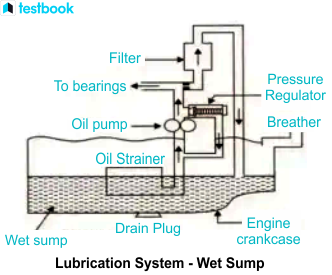
\includegraphics{lubrication-system-in-ic-engine.png}
\end{center}

\begin{itemize}[leftmargin=1.5em,itemsep=2pt]
  \item \textbf{Reduce friction and wear} between mating components.
  \item \textbf{Cooling:} Carries heat away from hot components (pistons,
        bearings).
  \item \textbf{Cleaning:} Suspends metallic particles and combustion by-products,
        carrying them to the filter.
  \item \textbf{Sealing:} Oil film between piston rings and cylinder wall reduces
        gas blow-by.
  \item \textbf{Cushioning:} Absorbs shock loads at crankshaft bearings.
  \item \textbf{Corrosion protection:} Oil film prevents oxidation of metal
        surfaces.
\end{itemize}

\hrulefill

\textbf{Part (b): Firing Order}

The \textbf{firing order} of a multi-cylinder engine is the sequence in which
the cylinders deliver their power strokes (fire). It is chosen to:
\begin{itemize}[leftmargin=1.5em,itemsep=2pt]
  \item Distribute the power impulses \emph{evenly} throughout each revolution,
        minimising torsional vibration on the crankshaft.
  \item Avoid consecutive firing of adjacent cylinders (which would cause
        one-sided loading).
  \item Provide a smooth, balanced torque output.
\end{itemize}

\textbf{Common examples:}
\begin{itemize}[leftmargin=1.5em,itemsep=1pt]
  \item Inline 4-cylinder: \textbf{1-3-4-2} or 1-2-4-3
  \item Inline 6-cylinder: \textbf{1-5-3-6-2-4}
  \item V8: \textbf{1-8-4-3-6-5-7-2} (common)
\end{itemize}

\end{tcolorbox}

\item \label{qlabel:A2-Q26}
(a) Explain with necessary sketches the sequence of operation of a 4-stroke SI engine. \mk{12}\\
(b) Draw the valve timing diagram of a 4-stroke diesel engine. \mk{8}\\
(c) Draw the indicator diagram of a 4-stroke SI engine. \mk{7}\\
(d) Why are inlet valves opened earlier and exhaust valves closed later w.r.t.\ TDC? \mk{8}
\yr{2005--06}

\begin{tcolorbox}[enhanced,breakable,ansbox,colback=cB!4,colframe=cB,
  boxrule=0.8pt,arc=5pt,
  title={\textbf{Answer}},fonttitle=\bfseries\color{white},colbacktitle=cB]

\textbf{Part (a):} \variant{A2-Q6 — identical; full answer with sketch given there}

\textbf{Part (b):}
\begin{center}
  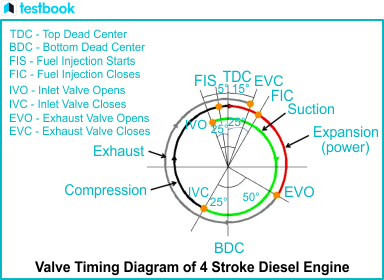
\includegraphics{valve-timing-diagram-of-4-stroke-diesel-engine.png}
\end{center}

\textbf{Part (c):} \variant{A2-Q20(b) — actual P-V indicator diagram given there}

\hrulefill

\textbf{Part (d): Why IVO Before TDC and EVC After TDC?}

\textbf{Inlet valve opens before TDC (IVO bTDC):}
\begin{itemize}[leftmargin=1.5em,itemsep=1pt]
  \item The inlet valve is a large mechanical component and takes finite time to
        reach full lift. Opening it early ensures it is \emph{fully open} by the
        time the piston reaches TDC and begins the intake stroke.
  \item This maximises the effective flow area during intake, improving
        volumetric efficiency.
\end{itemize}

\textbf{Exhaust valve closes after TDC (EVC aTDC):}
\begin{itemize}[leftmargin=1.5em,itemsep=1pt]
  \item The outward-flowing exhaust gas has \emph{inertia} (kinetic energy).
        Keeping the exhaust valve open past TDC allows this inertia to continue
        scavenging residual exhaust gas from the cylinder even after the piston
        starts moving back down.
  \item It also creates a slight suction effect that assists in drawing fresh
        charge through the inlet valve (which opens slightly before EVC —
        \emph{valve overlap}).
  \item Together, IVO bTDC and EVC aTDC create the valve overlap period that
        improves both exhaust scavenging and intake filling, boosting overall
        volumetric efficiency.
\end{itemize}

\end{tcolorbox}

%%────────────────────────────────────────────────────────────
%% A2-Q27
%%────────────────────────────────────────────────────────────
\item \label{qlabel:A2-Q27}
(a) An automobile engine is designated as ``1000\,cc'' --- what does this mean? \mk{5}\\
(b) Draw actual and ideal P-V diagrams of a 4-stroke SI engine. Why is pressure below atmospheric during the suction stroke in the actual cycle? \mk{15}\\
(c) Describe with a neat sketch the liquid cooling system of an IC engine. What is the purpose of a thermostat? \mk{15}
\yr{2004--05}

\begin{tcolorbox}[enhanced,breakable,ansbox,colback=cB!4,colframe=cB,
  boxrule=0.8pt,arc=5pt,
  title={\textbf{Answer}},fonttitle=\bfseries\color{white},colbacktitle=cB]

\textbf{Part (a): ``1000\,cc'' Engine}

The designation \textbf{1000\,cc} refers to the engine's \textbf{total swept
(displacement) volume} — the sum of the swept volumes of all cylinders:
\[
  V_{\text{total}} = n\times\frac{\pi}{4}d^2 L = 1000\,\text{cm}^3
\]
It represents the total volume swept by all pistons in one stroke from BDC to
TDC (or vice versa). It does \emph{not} include clearance volume. A larger cc
rating generally indicates a more powerful engine, as more fuel--air mixture can
be burned per cycle.

\hrulefill

\textbf{Part (b): Actual vs.\ Ideal P-V Diagrams}

\variant{A2-Q17(c) and A2-Q20(b) — both diagrams given in those answers}

\textbf{Why suction stroke pressure is below atmospheric in the actual cycle:}

In the ideal cycle, the suction stroke occurs exactly at atmospheric pressure.
However, in the actual cycle:
\begin{itemize}[leftmargin=1.5em,itemsep=2pt]
  \item The incoming air--fuel mixture must flow through the \textbf{throttle
        valve, air filter, carburettor/injector, and intake valve} — all of which
        create \textbf{flow resistance (pressure drop)}.
  \item This resistance means the pressure inside the cylinder during induction
        is \emph{below} atmospheric, typically by 10--30\,kPa depending on load
        and throttle position.
  \item The pressure difference drives the charge into the cylinder, but at a
        reduced cylinder pressure compared to ideal.
\end{itemize}
This effect is more pronounced at full throttle/high speed and reduces
volumetric efficiency.

\hrulefill

\textbf{Part (c): Liquid Cooling System and Thermostat}

\variant{A2-Q23(b) — same diagram given there}

\textbf{Purpose of the thermostat:}
The thermostat is a temperature-sensitive valve located between the engine and
radiator. Its functions are:
\begin{itemize}[leftmargin=1.5em,itemsep=2pt]
  \item \textbf{Rapid warm-up:} When the engine is cold, the thermostat remains
        \emph{closed}, bypassing the radiator. Coolant recirculates only within
        the engine, allowing it to reach operating temperature quickly
        ($\approx$80--95\textdegree C).
  \item \textbf{Temperature regulation:} Once the coolant reaches the thermostat
        opening temperature, it opens and allows coolant to flow through the
        radiator for cooling.
  \item \textbf{Efficiency:} Keeping the engine at the optimal operating
        temperature improves fuel combustion efficiency, reduces wear, and
        minimises emissions. A cold engine has higher friction and incomplete
        combustion.
\end{itemize}

\end{tcolorbox}

%%────────────────────────────────────────────────────────────
%% A2-Q28
%%────────────────────────────────────────────────────────────
\item \label{qlabel:A2-Q28}
(a) Draw a typical ignition circuit for a four-cylinder petrol engine. \mk{10}\\
(b) How is the liquid phase of coolant maintained in the cooling circuit? \mk{5}\\
(c) Why are four-stroke engines less harmful to the atmosphere than two-stroke engines? \mk{10}
\yr{2003--04}

\begin{tcolorbox}[enhanced,breakable,ansbox,colback=cB!4,colframe=cB,
  boxrule=0.8pt,arc=5pt,
  title={\textbf{Answer}},fonttitle=\bfseries\color{white},colbacktitle=cB]

\textbf{Part (a): Ignition Circuit — 4-Cylinder Petrol Engine}

\variant{A2-Q24(a) — same diagram given there}

\hrulefill

\textbf{Part (b): Maintaining Liquid Phase of Coolant}

The liquid phase is maintained by the following:
\begin{itemize}[leftmargin=1.5em,itemsep=2pt]
  \item \textbf{Pressurised cooling system:} The cooling system is sealed and
        pressurised (typically 0.9--1.2\,bar above atmospheric) using a
        \textbf{pressure cap} on the radiator or expansion tank. Increasing
        pressure raises the boiling point of the coolant (for every 14\,kPa of
        pressure, boiling point rises $\approx$3\textdegree C), allowing coolant
        to reach 120--130\textdegree C without boiling.
  \item \textbf{Antifreeze/coolant mixture:} Ethylene glycol mixed with water
        raises the boiling point and lowers the freezing point, maintaining
        liquid phase across a wider temperature range.
  \item \textbf{Expansion tank:} Accommodates thermal expansion of coolant,
        preventing pressure build-up from expelling coolant. The pressure cap
        also releases excess pressure if needed, and allows coolant to return
        from the expansion tank when cooling down.
\end{itemize}

\hrulefill

\textbf{Part (c): 4-Stroke vs.\ 2-Stroke — Environmental Impact}

Four-stroke engines are \textbf{less harmful to the atmosphere} than two-stroke
engines for the following reasons:

\begin{itemize}[leftmargin=1.5em,itemsep=3pt]
  \item \textbf{Dedicated exhaust stroke:} In a 4-stroke engine, a complete
        separate stroke is devoted to expelling exhaust gases. In a 2-stroke
        engine, exhaust and intake occur simultaneously (scavenging), and fresh
        charge inevitably mixes with and is expelled with exhaust gases —
        releasing unburnt hydrocarbons (HC) directly into the atmosphere.
  \item \textbf{No oil in fuel:} 2-stroke engines require oil to be mixed with
        fuel for crankcase lubrication. This oil is partially burned and
        partially expelled as visible blue smoke (unburnt oil), releasing harmful
        particulates and hydrocarbons. 4-stroke engines have a separate
        lubrication system.
  \item \textbf{Better combustion efficiency:} The 4-stroke cycle allows
        complete fuel combustion, producing primarily CO\textsubscript{2} and
        H\textsubscript{2}O. 2-stroke engines have lower combustion efficiency
        and higher CO and HC emissions.
  \item \textbf{Catalytic converter compatibility:} 4-stroke engines can
        effectively use catalytic converters to reduce HC, CO, and NO$_x$
        emissions. 2-stroke engines' oil-laden exhaust quickly poisons catalysts.
\end{itemize}

\end{tcolorbox}

%%────────────────────────────────────────────────────────────
%% A2-Q29
%%────────────────────────────────────────────────────────────

%% ============================================================
%%  Section A2 — IC Engines (Otto, Diesel Cycles)
%%  Question Bank — Answer Snippets
%%  Paste inside the A2 \begin{enumerate} ... \end{enumerate}
%% ============================================================

%%────────────────────────────────────────────────────────────
%% A2-Q1
%%────────────────────────────────────────────────────────────
\end{enumerate}

%%══════════════════════════════════════════════════════════════════════
%% SECTION A3 — Refrigeration & AC
%%══════════════════════════════════════════════════════════════════════
\secdivider{Section A3}{Refrigeration \& Air Conditioning}{cC}{cC}
\markboth{A3 --- Refrigeration \& Air Conditioning}{}
\label{sec:A3}
\titleformat{\section}{\large\bfseries\color{cC}}{}{0em}{}[\titlerule]
\section{A3 --- Refrigeration \& Air Conditioning}

\begin{enumerate}
\item \label{qlabel:A3-Q1}
(a) On the psychrometric chart, show how the dew-point temperature at a specified state is determined. \mk{5}\\
(b) Air at 1\,atm, 15\textdegree C and 60\% RH is heated to 20\textdegree C, then humidified to 25\textdegree C and 65\% RH. Determine: (i) steam added to air, (ii) heat transfer in the heating section. \mk{15}\\
(c) Draw a neat sketch of a split-type AC and mention its advantages and disadvantages. \mk{15}
\yr{2023--24}
\begin{center}
  
\includegraphics[height=0.3\textheight, width=0.75\textwidth,keepaspectratio]{/123.jpeg}
\end{center}

\begin{tcolorbox}[enhanced,breakable,ansbox,colback=cC!4,colframe=cC,
  boxrule=0.8pt,arc=5pt,
  title={\textbf{Answer}},fonttitle=\bfseries\color{white},colbacktitle=cC]

\textbf{Part (c): Split-Type Air Conditioner}

A split-type air conditioner divides the air conditioning system into two main components:
\begin{enumerate}[label=\arabic*., leftmargin=2em, itemsep=1pt]
    \item \textbf{Indoor Unit:} Installed inside the room, typically mounted on a wall. It contains the evaporator coil, a cross-flow cooling fan, and an air filter.
    \item \textbf{Outdoor Unit:} Installed outside the building. It houses the heavy and noisy components, including the compressor, condenser coil, condenser fan, and the expansion valve (or capillary tube).
\end{enumerate}
These two units are connected by insulated copper tubing (refrigerant lines) and electrical wiring.

\vspace{1em}
\begin{center}
  % Placeholder for your neat sketch
  
\includegraphics[height=0.3\textheight, width=0.75\textwidth,keepaspectratio]{/split.png}
\end{center}
\vspace{1em}

\textbf{Advantages:}
\begin{itemize}[label={--}, leftmargin=2em, itemsep=4pt]
  \item \textbf{Quiet Operation:} Because the compressor and condenser fan are located outdoors, the indoor noise level is significantly reduced compared to window units.
  \item \textbf{Aesthetics and Security:} The indoor unit is sleek and unobtrusive. It only requires a small hole (about 3 inches) in the wall for piping, avoiding the need to block a window or make a massive wall opening, which also preserves home security.
  \item \textbf{Cooling Capacity and Flexibility:} Can cool larger rooms effectively. They also offer multi-split configurations where a single outdoor unit can operate multiple indoor units in different rooms.
  \item \textbf{Better Air Distribution:} Wall-mounted indoor units are typically placed higher up, allowing for wider and more efficient dispersion of cold air throughout the room.
\end{itemize}

\textbf{Disadvantages:}
\begin{itemize}[label={--}, leftmargin=2em, itemsep=4pt]
  \item \textbf{Higher Initial Cost:} The purchase price of a split AC is generally higher than that of a window AC of the same capacity.
  \item \textbf{Complex Installation:} Requires professional installation to mount the units, route the refrigerant piping, and properly charge the system. It is not a DIY-friendly project.
  \item \textbf{Space Requirement:} You must have a suitable, well-ventilated outdoor space (like a balcony, roof, or exterior wall) to securely mount the heavy outdoor unit.
  \item \textbf{Maintenance Difficulties:} Troubleshooting and repairing can be more complex due to the separation of components and long refrigerant lines, which also pose a slightly higher risk of leaks over time.
\end{itemize}

\end{tcolorbox}


\item \label{qlabel:A3-Q2}
(a) A refrigerator uses R-134a on an ideal vapour compression cycle. Refrigerant evaporates at $-22$\textdegree C and condenses at 28\textdegree C. Mass flow rate\,$= 0.05$\,kg/s. Calculate: (i) rate of heat removal, (ii) power input to compressor, (iii) rate of heat rejection, (iv) COP. \mk{15}\\
(b) Define ``Refrigerant''. Mention desirable properties of a refrigerant. \mk{10}\\
(c) With a neat sketch of components, write a short note on Central Air Conditioning System. \mk{10}
\yr{2023--24}


\noindent\textbf{\Large TABLE A--11} \\
\noindent\textbf{\large Saturated refrigerant-134a---Temperature table}
\vspace{0.3cm}

\begin{center}
\small
\begin{longtable}{c c c c c c c c c c c c c}
\toprule\toprule
& & \multicolumn{2}{c}{\textit{Specific volume,}} & \multicolumn{3}{c}{\textit{Internal energy,}} & \multicolumn{3}{c}{\textit{Enthalpy,}} & \multicolumn{3}{c}{\textit{Entropy,}} \\
& & \multicolumn{2}{c}{$\text{m}^3\text{/kg}$} & \multicolumn{3}{c}{$\text{kJ/kg}$} & \multicolumn{3}{c}{$\text{kJ/kg}$} & \multicolumn{3}{c}{$\text{kJ/kg}\cdot\text{K}$} \\
\cmidrule(lr){3-4} \cmidrule(lr){5-7} \cmidrule(lr){8-10} \cmidrule(lr){11-13}
& Sat. & Sat. & Sat. & Sat. & & Sat. & Sat. & & Sat. & Sat. & & Sat. \\
Temp., & press., & liquid, & vapor, & liquid, & Evap., & vapor, & liquid, & Evap., & vapor, & liquid, & Evap., & vapor, \\
$T^\circ\text{C}$ & $P_{\text{sat}}$ kPa & $v_f$ & $v_g$ & $u_f$ & $u_{fg}$ & $u_g$ & $h_f$ & $h_{fg}$ & $h_g$ & $s_f$ & $s_{fg}$ & $s_g$ \\
\midrule
\endhead

\midrule
\multicolumn{13}{r}{{Continued on next page}} \\
\bottomrule
\endfoot

\bottomrule\bottomrule
\endlastfoot

-40 & 51.25 & 0.0007054 & 0.36081 & -0.036 & 207.40 & 207.37 & 0.000 & 225.86 & 225.86 & 0.00000 & 0.96866 & 0.96866 \\
-38 & 56.86 & 0.0007083 & 0.32732 & 2.475 & 206.04 & 208.51 & 2.515 & 224.61 & 227.12 & 0.01072 & 0.95511 & 0.96584 \\
-36 & 62.95 & 0.0007112 & 0.29751 & 4.992 & 204.67 & 209.66 & 5.037 & 223.35 & 228.39 & 0.02138 & 0.94176 & 0.96315 \\
-34 & 69.56 & 0.0007142 & 0.27090 & 7.517 & 203.29 & 210.81 & 7.566 & 222.09 & 229.65 & 0.03199 & 0.92859 & 0.96058 \\
-32 & 76.71 & 0.0007172 & 0.24711 & 10.05 & 201.91 & 211.96 & 10.10 & 220.81 & 230.91 & 0.04253 & 0.91560 & 0.95813 \\
\addlinespace
-30 & 84.43 & 0.0007203 & 0.22580 & 12.59 & 200.52 & 213.11 & 12.65 & 219.52 & 232.17 & 0.05301 & 0.90278 & 0.95579 \\
-28 & 92.76 & 0.0007234 & 0.20666 & 15.13 & 199.12 & 214.25 & 15.20 & 218.22 & 233.43 & 0.06344 & 0.89012 & 0.95356 \\
-26 & 101.73 & 0.0007265 & 0.18946 & 17.69 & 197.72 & 215.40 & 17.76 & 216.92 & 234.68 & 0.07382 & 0.87762 & 0.95144 \\
-24 & 111.37 & 0.0007297 & 0.17395 & 20.25 & 196.30 & 216.55 & 20.33 & 215.59 & 235.92 & 0.08414 & 0.86527 & 0.94941 \\
-22 & 121.72 & 0.0007329 & 0.15995 & 22.82 & 194.88 & 217.70 & 22.91 & 214.26 & 237.17 & 0.09441 & 0.85307 & 0.94748 \\
\addlinespace
-20 & 132.82 & 0.0007362 & 0.14729 & 25.39 & 193.45 & 218.84 & 25.49 & 212.91 & 238.41 & 0.10463 & 0.84101 & 0.94564 \\
-18 & 144.69 & 0.0007396 & 0.13583 & 27.98 & 192.01 & 219.98 & 28.09 & 211.55 & 239.64 & 0.11481 & 0.82908 & 0.94389 \\
-16 & 157.38 & 0.0007430 & 0.12542 & 30.57 & 190.56 & 221.13 & 30.69 & 210.18 & 240.87 & 0.12493 & 0.81729 & 0.94222 \\
-14 & 170.93 & 0.0007464 & 0.11597 & 33.17 & 189.09 & 222.27 & 33.30 & 208.79 & 242.09 & 0.13501 & 0.80561 & 0.94063 \\
-12 & 185.37 & 0.0007499 & 0.10736 & 35.78 & 187.62 & 223.40 & 35.92 & 207.38 & 243.30 & 0.14504 & 0.79406 & 0.93911 \\
\addlinespace
-10 & 200.74 & 0.0007535 & 0.099516 & 38.40 & 186.14 & 224.54 & 38.55 & 205.96 & 244.51 & 0.15504 & 0.78263 & 0.93766 \\
-8 & 217.08 & 0.0007571 & 0.092352 & 41.03 & 184.64 & 225.67 & 41.19 & 204.52 & 245.72 & 0.16498 & 0.77130 & 0.93629 \\
-6 & 234.44 & 0.0007608 & 0.085802 & 43.66 & 183.13 & 226.80 & 43.84 & 203.07 & 246.91 & 0.17489 & 0.76008 & 0.93497 \\
-4 & 252.85 & 0.0007646 & 0.079804 & 46.31 & 181.61 & 227.92 & 46.50 & 201.60 & 248.10 & 0.18476 & 0.74896 & 0.93372 \\
-2 & 272.36 & 0.0007684 & 0.074304 & 48.96 & 180.08 & 229.04 & 49.17 & 200.11 & 249.28 & 0.19459 & 0.73794 & 0.93253 \\
\addlinespace
0 & 293.01 & 0.0007723 & 0.069255 & 51.63 & 178.53 & 230.16 & 51.86 & 198.60 & 250.45 & 0.20439 & 0.72701 & 0.93139 \\
2 & 314.84 & 0.0007763 & 0.064612 & 54.30 & 176.97 & 231.27 & 54.55 & 197.07 & 251.61 & 0.21415 & 0.71616 & 0.93031 \\
4 & 337.90 & 0.0007804 & 0.060338 & 56.99 & 175.39 & 232.38 & 57.25 & 195.51 & 252.77 & 0.22387 & 0.70540 & 0.92927 \\
6 & 362.23 & 0.0007845 & 0.056398 & 59.68 & 173.80 & 233.48 & 59.97 & 193.94 & 253.91 & 0.23356 & 0.69471 & 0.92828 \\
8 & 387.88 & 0.0007887 & 0.052762 & 62.39 & 172.19 & 234.58 & 62.69 & 192.35 & 255.04 & 0.24323 & 0.68410 & 0.92733 \\
\addlinespace
10 & 414.89 & 0.0007930 & 0.049403 & 65.10 & 170.56 & 235.67 & 65.43 & 190.73 & 256.16 & 0.25286 & 0.67356 & 0.92641 \\
12 & 443.31 & 0.0007975 & 0.046295 & 67.83 & 168.92 & 236.75 & 68.18 & 189.09 & 257.27 & 0.26246 & 0.66308 & 0.92554 \\
14 & 473.19 & 0.0008020 & 0.043417 & 70.57 & 167.26 & 237.83 & 70.95 & 187.42 & 258.37 & 0.27204 & 0.65266 & 0.92470 \\
16 & 504.58 & 0.0008066 & 0.040748 & 73.32 & 165.58 & 238.90 & 73.73 & 185.73 & 259.46 & 0.28159 & 0.64230 & 0.92389 \\
18 & 537.52 & 0.0008113 & 0.038271 & 76.08 & 163.88 & 239.96 & 76.52 & 184.01 & 260.53 & 0.29112 & 0.63198 & 0.92310 \\
\addlinespace
20 & 572.07 & 0.0008161 & 0.035969 & 78.86 & 162.16 & 241.02 & 79.32 & 182.27 & 261.59 & 0.30063 & 0.62172 & 0.92234 \\
22 & 608.27 & 0.0008210 & 0.033828 & 81.64 & 160.42 & 242.06 & 82.14 & 180.49 & 262.64 & 0.31011 & 0.61149 & 0.92160 \\
24 & 646.18 & 0.0008261 & 0.031834 & 84.44 & 158.65 & 243.10 & 84.98 & 178.69 & 263.67 & 0.31958 & 0.60130 & 0.92088 \\
26 & 685.84 & 0.0008313 & 0.029976 & 87.26 & 156.87 & 244.12 & 87.83 & 176.85 & 264.68 & 0.32903 & 0.59115 & 0.92018 \\
28 & 727.31 & 0.0008366 & 0.028242 & 90.09 & 155.05 & 245.14 & 90.69 & 174.99 & 265.68 & 0.33846 & 0.58102 & 0.91948 \\
\addlinespace
30 & 770.64 & 0.0008421 & 0.026622 & 92.93 & 153.22 & 246.14 & 93.58 & 173.08 & 266.66 & 0.34789 & 0.57091 & 0.91879 \\
32 & 815.89 & 0.0008478 & 0.025108 & 95.79 & 151.35 & 247.14 & 96.48 & 171.14 & 267.62 & 0.35730 & 0.56082 & 0.91811 \\
34 & 863.11 & 0.0008536 & 0.023691 & 98.66 & 149.46 & 248.12 & 99.40 & 169.17 & 268.57 & 0.36670 & 0.55074 & 0.91743 \\
36 & 912.35 & 0.0008595 & 0.022364 & 101.55 & 147.54 & 249.08 & 102.33 & 167.16 & 269.49 & 0.37609 & 0.54066 & 0.91675 \\
38 & 963.68 & 0.0008657 & 0.021119 & 104.45 & 145.58 & 250.04 & 105.29 & 165.10 & 270.39 & 0.38548 & 0.53058 & 0.91606 \\
\addlinespace
40 & 1017.1 & 0.0008720 & 0.019952 & 107.38 & 143.60 & 250.97 & 108.26 & 163.00 & 271.27 & 0.39486 & 0.52049 & 0.91536 \\
42 & 1072.8 & 0.0008786 & 0.018855 & 110.32 & 141.58 & 251.89 & 111.26 & 160.86 & 272.12 & 0.40425 & 0.51039 & 0.91464 \\
44 & 1130.7 & 0.0008854 & 0.017824 & 113.28 & 139.52 & 252.80 & 114.28 & 158.67 & 272.95 & 0.41363 & 0.50027 & 0.91391 \\
46 & 1191.0 & 0.0008924 & 0.016853 & 116.26 & 137.42 & 253.68 & 117.32 & 156.43 & 273.75 & 0.42302 & 0.49012 & 0.91315 \\
48 & 1253.6 & 0.0008996 & 0.015939 & 119.26 & 135.29 & 254.55 & 120.39 & 154.14 & 274.53 & 0.43242 & 0.47993 & 0.91236 \\
\addlinespace
52 & 1386.2 & 0.0009150 & 0.014265 & 125.33 & 130.88 & 256.21 & 126.59 & 149.39 & 275.98 & 0.45126 & 0.45941 & 0.91067 \\
56 & 1529.1 & 0.0009317 & 0.012771 & 131.49 & 126.28 & 257.77 & 132.91 & 144.38 & 277.30 & 0.47018 & 0.43863 & 0.90880 \\
60 & 1682.8 & 0.0009498 & 0.011434 & 137.76 & 121.46 & 259.22 & 139.36 & 139.10 & 278.46 & 0.48920 & 0.41749 & 0.90669 \\
65 & 1891.0 & 0.0009750 & 0.009950 & 145.77 & 115.05 & 260.82 & 147.62 & 132.02 & 279.64 & 0.51320 & 0.39039 & 0.90359 \\
70 & 2118.2 & 0.0010037 & 0.008642 & 154.01 & 108.14 & 262.15 & 156.13 & 124.32 & 280.46 & 0.53755 & 0.36227 & 0.89982 \\
75 & 2365.8 & 0.0010372 & 0.007480 & 162.53 & 100.60 & 263.13 & 164.98 & 115.85 & 280.82 & 0.56241 & 0.33272 & 0.89512 \\
\addlinespace
80 & 2635.3 & 0.0010772 & 0.006436 & 171.40 & 92.23 & 263.63 & 174.24 & 106.35 & 280.59 & 0.58800 & 0.30111 & 0.88912 \\
85 & 2928.2 & 0.0011270 & 0.005486 & 180.77 & 82.67 & 263.44 & 184.07 & 95.44 & 279.51 & 0.61473 & 0.26644 & 0.88117 \\
90 & 3246.9 & 0.0011932 & 0.004599 & 190.89 & 71.29 & 262.18 & 194.76 & 82.35 & 277.11 & 0.64336 & 0.22674 & 0.87010 \\
95 & 3594.1 & 0.0012933 & 0.003726 & 202.40 & 56.47 & 258.87 & 207.05 & 65.21 & 272.26 & 0.67578 & 0.17711 & 0.85289 \\
100 & 3975.1 & 0.0015269 & 0.002630 & 218.72 & 29.19 & 247.91 & 224.79 & 33.58 & 258.37 & 0.72217 & 0.08999 & 0.81215 \\
\end{longtable}

\vspace{0.2cm}
\noindent\scriptsize \textit{Source:} Tables A--11 through A--13 are generated using the Engineering Equation Solver (EES) software developed by S. A. Klein and F. L. Alvarado. The routine used in calculations is the R134a, which is based on the fundamental equation of state developed by R. Tillner-Roth and H.D. Baehr, ``An International Standard Formulation for the Thermodynamic Properties of 1,1,1,2-Tetrafluoroethane (HFC-134a) for temperatures from 170 K to 455 K and Pressures up to 70 MPa,'' \textit{J. Phys. Chem, Ref. Data}, Vol. 23, No. 5, 1994. The enthalpy and entropy values of saturated liquid are set to zero at $-40^\circ\text{C}$ (and $-40^\circ\text{F}$).

\end{center}

\noindent\textbf{\Large TABLE A--12} \\
\noindent\textbf{\large Saturated refrigerant-134a---Pressure table}
\vspace{0.3cm}

\begin{center}
\small
\begin{longtable}{c c c c c c c c c c c c c}
\toprule\toprule
& & \multicolumn{2}{c}{\textit{Specific volume,}} & \multicolumn{3}{c}{\textit{Internal energy,}} & \multicolumn{3}{c}{\textit{Enthalpy,}} & \multicolumn{3}{c}{\textit{Entropy,}} \\
& & \multicolumn{2}{c}{$\text{m}^3\text{/kg}$} & \multicolumn{3}{c}{$\text{kJ/kg}$} & \multicolumn{3}{c}{$\text{kJ/kg}$} & \multicolumn{3}{c}{$\text{kJ/kg}\cdot\text{K}$} \\
\cmidrule(lr){3-4} \cmidrule(lr){5-7} \cmidrule(lr){8-10} \cmidrule(lr){11-13}
& Sat. & Sat. & Sat. & Sat. & & Sat. & Sat. & & Sat. & Sat. & & Sat. \\
Press., & temp., & liquid, & vapor, & liquid, & Evap., & vapor, & liquid, & Evap., & vapor, & liquid, & Evap., & vapor, \\
$P$ kPa & $T_{\text{sat}}$ $^\circ\text{C}$ & $v_f$ & $v_g$ & $u_f$ & $u_{fg}$ & $u_g$ & $h_f$ & $h_{fg}$ & $h_g$ & $s_f$ & $s_{fg}$ & $s_g$ \\
\midrule
\endhead

\midrule
\multicolumn{13}{r}{{Continued on next page}} \\
\bottomrule
\endfoot

\bottomrule\bottomrule
\endlastfoot

60 & -36.95 & 0.0007098 & 0.31121 & 3.798 & 205.32 & 209.12 & 3.841 & 223.95 & 227.79 & 0.01634 & 0.94807 & 0.96441 \\
70 & -33.87 & 0.0007144 & 0.26929 & 7.680 & 203.20 & 210.88 & 7.730 & 222.00 & 229.73 & 0.03267 & 0.92775 & 0.96042 \\
80 & -31.13 & 0.0007185 & 0.23753 & 11.15 & 201.30 & 212.46 & 11.21 & 220.25 & 231.46 & 0.04711 & 0.90999 & 0.95710 \\
90 & -28.65 & 0.0007223 & 0.21263 & 14.31 & 199.57 & 213.88 & 14.37 & 218.65 & 233.02 & 0.06008 & 0.89419 & 0.95427 \\
100 & -26.37 & 0.0007259 & 0.19254 & 17.21 & 197.98 & 215.19 & 17.28 & 217.16 & 234.44 & 0.07188 & 0.87995 & 0.95183 \\
\addlinespace
120 & -22.32 & 0.0007324 & 0.16212 & 22.40 & 195.11 & 217.51 & 22.49 & 214.48 & 236.97 & 0.09275 & 0.85503 & 0.94779 \\
140 & -18.77 & 0.0007383 & 0.14014 & 26.98 & 192.57 & 219.54 & 27.08 & 212.08 & 239.16 & 0.11087 & 0.83368 & 0.94456 \\
160 & -15.60 & 0.0007437 & 0.12348 & 31.09 & 190.27 & 221.35 & 31.21 & 209.90 & 241.11 & 0.12693 & 0.81496 & 0.94190 \\
180 & -12.73 & 0.0007487 & 0.11041 & 34.83 & 188.16 & 222.99 & 34.97 & 207.90 & 242.86 & 0.14139 & 0.79826 & 0.93965 \\
200 & -10.09 & 0.0007533 & 0.099867 & 38.28 & 186.21 & 224.48 & 38.43 & 206.03 & 244.46 & 0.15457 & 0.78316 & 0.93773 \\
\addlinespace
240 & -5.38 & 0.0007620 & 0.083897 & 44.48 & 182.67 & 227.14 & 44.66 & 202.62 & 247.28 & 0.17794 & 0.75664 & 0.93458 \\
280 & -1.25 & 0.0007699 & 0.072352 & 49.97 & 179.50 & 229.46 & 50.18 & 199.54 & 249.72 & 0.19829 & 0.73381 & 0.93210 \\
320 & 2.46 & 0.0007772 & 0.063604 & 54.92 & 176.61 & 231.52 & 55.16 & 196.71 & 251.88 & 0.21637 & 0.71369 & 0.93006 \\
360 & 5.82 & 0.0007841 & 0.056738 & 59.44 & 173.94 & 233.38 & 59.72 & 194.08 & 253.81 & 0.23270 & 0.69566 & 0.92836 \\
400 & 8.91 & 0.0007907 & 0.051201 & 63.62 & 171.45 & 235.07 & 63.94 & 191.62 & 255.55 & 0.24761 & 0.67929 & 0.92691 \\
\addlinespace
450 & 12.46 & 0.0007985 & 0.045619 & 68.45 & 168.54 & 237.00 & 68.81 & 188.71 & 257.53 & 0.26465 & 0.66069 & 0.92535 \\
500 & 15.71 & 0.0008059 & 0.041118 & 72.93 & 165.82 & 238.75 & 73.33 & 185.98 & 259.30 & 0.28023 & 0.64377 & 0.92400 \\
550 & 18.73 & 0.0008130 & 0.037408 & 77.10 & 163.25 & 240.35 & 77.54 & 183.38 & 260.92 & 0.29461 & 0.62821 & 0.92282 \\
600 & 21.55 & 0.0008199 & 0.034295 & 81.02 & 160.81 & 241.83 & 81.51 & 180.90 & 262.40 & 0.30799 & 0.61378 & 0.92177 \\
650 & 24.20 & 0.0008266 & 0.031646 & 84.72 & 158.48 & 243.20 & 85.26 & 178.51 & 263.77 & 0.32051 & 0.60030 & 0.92081 \\
\addlinespace
700 & 26.69 & 0.0008331 & 0.029361 & 88.24 & 156.24 & 244.48 & 88.82 & 176.21 & 265.03 & 0.33230 & 0.58763 & 0.91994 \\
750 & 29.06 & 0.0008395 & 0.027371 & 91.59 & 154.08 & 245.67 & 92.22 & 173.98 & 266.20 & 0.34345 & 0.57567 & 0.91912 \\
800 & 31.31 & 0.0008458 & 0.025621 & 94.79 & 152.00 & 246.79 & 95.47 & 171.82 & 267.29 & 0.35404 & 0.56431 & 0.91835 \\
850 & 33.45 & 0.0008520 & 0.024069 & 97.87 & 149.98 & 247.85 & 98.60 & 169.71 & 268.31 & 0.36413 & 0.55349 & 0.91762 \\
\addlinespace
900 & 35.51 & 0.0008580 & 0.022683 & 100.83 & 148.01 & 248.85 & 101.61 & 167.66 & 269.26 & 0.37377 & 0.54315 & 0.91692 \\
950 & 37.48 & 0.0008641 & 0.021438 & 103.69 & 146.10 & 249.79 & 104.51 & 165.64 & 270.15 & 0.38301 & 0.53323 & 0.91624 \\
1000 & 39.37 & 0.0008700 & 0.020313 & 106.45 & 144.23 & 250.68 & 107.32 & 163.67 & 270.99 & 0.39189 & 0.52368 & 0.91558 \\
1200 & 46.29 & 0.0008934 & 0.016715 & 116.70 & 137.11 & 253.81 & 117.77 & 156.10 & 273.87 & 0.42441 & 0.48863 & 0.91303 \\
1400 & 52.40 & 0.0009166 & 0.014107 & 125.94 & 130.43 & 256.37 & 127.22 & 148.90 & 276.12 & 0.45315 & 0.45734 & 0.91050 \\
\addlinespace
1600 & 57.88 & 0.0009400 & 0.012123 & 134.43 & 124.04 & 258.47 & 135.93 & 141.93 & 277.86 & 0.47911 & 0.42873 & 0.90784 \\
1800 & 62.87 & 0.0009639 & 0.010559 & 142.33 & 117.83 & 260.17 & 144.07 & 135.11 & 279.17 & 0.50294 & 0.40204 & 0.90498 \\
2000 & 67.45 & 0.0009886 & 0.009288 & 149.78 & 111.73 & 261.51 & 151.76 & 128.33 & 280.09 & 0.52509 & 0.37675 & 0.90184 \\
2500 & 77.54 & 0.0010566 & 0.006936 & 166.99 & 96.47 & 263.45 & 169.63 & 111.16 & 280.79 & 0.57531 & 0.31695 & 0.89226 \\
3000 & 86.16 & 0.0011406 & 0.005275 & 183.04 & 80.22 & 263.26 & 186.46 & 92.63 & 279.09 & 0.62118 & 0.25776 & 0.87894 \\
\end{longtable}
\end{center}


\noindent\textbf{\Large TABLE A--13} \\
\noindent\textbf{\large Superheated refrigerant-134a}
\vspace{0.3cm}

\begin{center}
\small
\begin{longtable}{@{} c *{3}{@{\hspace{12pt}} c c c c} @{}}
\toprule\toprule
$T$ & $v$ & $u$ & $h$ & $s$ & $v$ & $u$ & $h$ & $s$ & $v$ & $u$ & $h$ & $s$ \\
$^\circ\text{C}$ & $\text{m}^3\text{/kg}$ & $\text{kJ/kg}$ & $\text{kJ/kg}$ & $\text{kJ/kg}\cdot\text{K}$ & $\text{m}^3\text{/kg}$ & $\text{kJ/kg}$ & $\text{kJ/kg}$ & $\text{kJ/kg}\cdot\text{K}$ & $\text{m}^3\text{/kg}$ & $\text{kJ/kg}$ & $\text{kJ/kg}$ & $\text{kJ/kg}\cdot\text{K}$ \\
\midrule
\endhead

\midrule
\multicolumn{13}{r}{{Continued on next page}} \\
\bottomrule
\endfoot

\bottomrule\bottomrule
\endlastfoot

% ----------------- BLOCK 1 -----------------
& \multicolumn{4}{c}{\textit{$P = 0.06$ MPa ($T_{\text{sat}} = -36.95^\circ\text{C}$)}} 
& \multicolumn{4}{c}{\textit{$P = 0.10$ MPa ($T_{\text{sat}} = -26.37^\circ\text{C}$)}} 
& \multicolumn{4}{c}{\textit{$P = 0.14$ MPa ($T_{\text{sat}} = -18.77^\circ\text{C}$)}} \\
\cmidrule(lr){2-5} \cmidrule(lr){6-9} \cmidrule(lr){10-13}
Sat. & 0.31121 & 209.12 & 227.79 & 0.9644 & 0.19254 & 215.19 & 234.44 & 0.9518 & 0.14014 & 219.54 & 239.16 & 0.9446 \\
-20  & 0.33608 & 220.60 & 240.76 & 1.0174 & 0.19841 & 219.66 & 239.50 & 0.9721 & & & & \\
-10  & 0.35048 & 227.55 & 248.58 & 1.0477 & 0.20743 & 226.75 & 247.49 & 1.0030 & 0.14605 & 225.91 & 246.36 & 0.9724 \\
0    & 0.36476 & 234.66 & 256.54 & 1.0774 & 0.21630 & 233.95 & 255.58 & 1.0332 & 0.15263 & 233.23 & 254.60 & 1.0031 \\
10   & 0.37893 & 241.92 & 264.66 & 1.1066 & 0.22506 & 241.30 & 263.81 & 1.0628 & 0.15908 & 240.66 & 262.93 & 1.0331 \\
20   & 0.39302 & 249.35 & 272.94 & 1.1353 & 0.23373 & 248.79 & 272.17 & 1.0918 & 0.16544 & 248.22 & 271.38 & 1.0624 \\
30   & 0.40705 & 256.95 & 281.37 & 1.1636 & 0.24233 & 256.44 & 280.68 & 1.1203 & 0.17172 & 255.93 & 279.97 & 1.0912 \\
40   & 0.42102 & 264.71 & 289.97 & 1.1915 & 0.25088 & 264.25 & 289.34 & 1.1484 & 0.17794 & 263.79 & 288.70 & 1.1195 \\
50   & 0.43495 & 272.64 & 298.74 & 1.2191 & 0.25937 & 272.22 & 298.16 & 1.1762 & 0.18412 & 271.79 & 297.57 & 1.1474 \\
60   & 0.44883 & 280.73 & 307.66 & 1.2463 & 0.26783 & 280.35 & 307.13 & 1.2035 & 0.19025 & 279.96 & 306.59 & 1.1749 \\
70   & 0.46269 & 288.99 & 316.75 & 1.2732 & 0.27626 & 288.64 & 316.26 & 1.2305 & 0.19635 & 288.28 & 315.77 & 1.2020 \\
80   & 0.47651 & 297.41 & 326.00 & 1.2997 & 0.28465 & 297.08 & 325.55 & 1.2572 & 0.20242 & 296.75 & 325.09 & 1.2288 \\
90   & 0.49032 & 306.00 & 335.42 & 1.3260 & 0.29303 & 305.69 & 334.99 & 1.2836 & 0.20847 & 305.38 & 334.57 & 1.2553 \\
100  & 0.50410 & 314.74 & 344.99 & 1.3520 & 0.30138 & 314.46 & 344.60 & 1.3096 & 0.21449 & 314.17 & 344.20 & 1.2814 \\
\midrule

% ----------------- BLOCK 2 -----------------
& \multicolumn{4}{c}{\textit{$P = 0.18$ MPa ($T_{\text{sat}} = -12.73^\circ\text{C}$)}} 
& \multicolumn{4}{c}{\textit{$P = 0.20$ MPa ($T_{\text{sat}} = -10.09^\circ\text{C}$)}} 
& \multicolumn{4}{c}{\textit{$P = 0.24$ MPa ($T_{\text{sat}} = -5.38^\circ\text{C}$)}} \\
\cmidrule(lr){2-5} \cmidrule(lr){6-9} \cmidrule(lr){10-13}
Sat. & 0.11041 & 222.99 & 242.86 & 0.9397 & 0.09987 & 224.48 & 244.46 & 0.9377 & 0.08390 & 227.14 & 247.28 & 0.9346 \\
-10  & 0.11189 & 225.02 & 245.16 & 0.9484 & 0.09991 & 224.55 & 244.54 & 0.9380 & & & & \\
0    & 0.11722 & 232.48 & 253.58 & 0.9798 & 0.10481 & 232.09 & 253.05 & 0.9698 & 0.08617 & 231.29 & 251.97 & 0.9519 \\
10   & 0.12240 & 240.00 & 262.04 & 1.0102 & 0.10955 & 239.67 & 261.58 & 1.0004 & 0.09026 & 238.98 & 260.65 & 0.9831 \\
20   & 0.12748 & 247.64 & 270.59 & 1.0399 & 0.11418 & 247.35 & 270.18 & 1.0303 & 0.09423 & 246.74 & 269.36 & 1.0134 \\
30   & 0.13248 & 255.41 & 279.25 & 1.0690 & 0.11874 & 255.14 & 278.89 & 1.0595 & 0.09812 & 254.61 & 278.16 & 1.0429 \\
40   & 0.13741 & 263.31 & 288.05 & 1.0975 & 0.12322 & 263.08 & 287.72 & 1.0882 & 0.10193 & 262.59 & 287.06 & 1.0718 \\
50   & 0.14230 & 271.36 & 296.98 & 1.1256 & 0.12766 & 271.15 & 296.68 & 1.1163 & 0.10570 & 270.71 & 296.08 & 1.1001 \\
60   & 0.14715 & 279.56 & 306.05 & 1.1532 & 0.13206 & 279.37 & 305.78 & 1.1441 & 0.10942 & 278.97 & 305.23 & 1.1280 \\
70   & 0.15196 & 287.91 & 315.27 & 1.1805 & 0.13641 & 287.73 & 315.01 & 1.1714 & 0.11310 & 287.36 & 314.51 & 1.1554 \\
80   & 0.15673 & 296.42 & 324.63 & 1.2074 & 0.14074 & 296.25 & 324.40 & 1.1983 & 0.11675 & 295.91 & 323.93 & 1.1825 \\
90   & 0.16149 & 305.07 & 334.14 & 1.2339 & 0.14504 & 304.92 & 333.93 & 1.2249 & 0.12038 & 304.60 & 333.49 & 1.2092 \\
100  & 0.16622 & 313.88 & 343.80 & 1.2602 & 0.14933 & 313.74 & 343.60 & 1.2512 & 0.12398 & 313.44 & 343.20 & 1.2356 \\
\midrule

% ----------------- BLOCK 3 -----------------
& \multicolumn{4}{c}{\textit{$P = 0.28$ MPa ($T_{\text{sat}} = -1.25^\circ\text{C}$)}} 
& \multicolumn{4}{c}{\textit{$P = 0.32$ MPa ($T_{\text{sat}} = 2.46^\circ\text{C}$)}} 
& \multicolumn{4}{c}{\textit{$P = 0.40$ MPa ($T_{\text{sat}} = 8.91^\circ\text{C}$)}} \\
\cmidrule(lr){2-5} \cmidrule(lr){6-9} \cmidrule(lr){10-13}
Sat. & 0.07235 & 229.46 & 249.72 & 0.9321 & 0.06360 & 231.52 & 251.88 & 0.9301 & 0.051201 & 235.07 & 255.55 & 0.9269 \\
0    & 0.07282 & 230.44 & 250.83 & 0.9362 & & & & & & & & \\
10   & 0.07646 & 238.27 & 259.68 & 0.9680 & 0.06609 & 237.54 & 258.69 & 0.9544 & 0.051506 & 235.97 & 256.58 & 0.9305 \\
20   & 0.07997 & 246.13 & 268.52 & 0.9987 & 0.06925 & 245.50 & 267.66 & 0.9856 & 0.054213 & 244.18 & 265.86 & 0.9628 \\
30   & 0.08338 & 254.06 & 277.41 & 1.0285 & 0.07231 & 253.50 & 276.65 & 1.0157 & 0.056796 & 252.36 & 275.07 & 0.9937 \\
40   & 0.08672 & 262.10 & 286.38 & 1.0576 & 0.07530 & 261.60 & 285.70 & 1.0451 & 0.059292 & 260.58 & 284.30 & 1.0236 \\
50   & 0.09000 & 270.27 & 295.47 & 1.0862 & 0.07823 & 269.82 & 294.85 & 1.0739 & 0.061724 & 268.90 & 293.59 & 1.0528 \\
60   & 0.09324 & 278.56 & 304.67 & 1.1142 & 0.08111 & 278.15 & 304.11 & 1.1021 & 0.064104 & 277.32 & 302.96 & 1.0814 \\
70   & 0.09644 & 286.99 & 314.00 & 1.1418 & 0.08395 & 286.62 & 313.48 & 1.1298 & 0.066443 & 285.86 & 312.44 & 1.1094 \\
80   & 0.09961 & 295.57 & 323.46 & 1.1690 & 0.08675 & 295.22 & 322.98 & 1.1571 & 0.068747 & 294.53 & 322.02 & 1.1369 \\
90   & 0.10275 & 304.29 & 333.06 & 1.1958 & 0.08953 & 303.97 & 332.62 & 1.1840 & 0.071023 & 303.32 & 331.73 & 1.1640 \\
100  & 0.10587 & 313.15 & 342.80 & 1.2222 & 0.09229 & 312.86 & 342.39 & 1.2105 & 0.073274 & 312.26 & 341.57 & 1.1907 \\
110  & 0.10897 & 322.16 & 352.68 & 1.2483 & 0.09503 & 321.89 & 352.30 & 1.2367 & 0.075504 & 321.33 & 351.53 & 1.2171 \\
120  & 0.11205 & 331.32 & 362.70 & 1.2742 & 0.09775 & 331.07 & 362.35 & 1.2626 & 0.077717 & 330.55 & 361.63 & 1.2431 \\
130  & 0.11512 & 340.63 & 372.87 & 1.2997 & 0.10045 & 340.39 & 372.54 & 1.2882 & 0.079913 & 339.90 & 371.87 & 1.2688 \\
140  & 0.11818 & 350.09 & 383.18 & 1.3250 & 0.10314 & 349.86 & 382.87 & 1.3135 & 0.082096 & 349.41 & 382.24 & 1.2942 \\
\midrule

% ----------------- BLOCK 4 -----------------
& \multicolumn{4}{c}{\textit{$P = 0.50$ MPa ($T_{\text{sat}} = 15.71^\circ\text{C}$)}} 
& \multicolumn{4}{c}{\textit{$P = 0.60$ MPa ($T_{\text{sat}} = 21.55^\circ\text{C}$)}} 
& \multicolumn{4}{c}{\textit{$P = 0.70$ MPa ($T_{\text{sat}} = 26.69^\circ\text{C}$)}} \\
\cmidrule(lr){2-5} \cmidrule(lr){6-9} \cmidrule(lr){10-13}
Sat. & 0.041118 & 238.75 & 259.30 & 0.9240 & 0.034295 & 241.83 & 262.40 & 0.9218 & 0.029361 & 244.48 & 265.03 & 0.9199 \\
20   & 0.042115 & 242.40 & 263.46 & 0.9383 & & & & & & & & \\
30   & 0.044338 & 250.84 & 273.01 & 0.9703 & 0.035984 & 249.22 & 270.81 & 0.9499 & 0.029966 & 247.48 & 268.45 & 0.9313 \\
40   & 0.046456 & 259.26 & 282.48 & 1.0011 & 0.037865 & 257.86 & 280.58 & 0.9816 & 0.031696 & 256.39 & 278.57 & 0.9641 \\
50   & 0.048499 & 267.72 & 291.96 & 1.0309 & 0.039659 & 266.48 & 290.28 & 1.0121 & 0.033322 & 265.20 & 288.53 & 0.9954 \\
60   & 0.050485 & 276.25 & 301.50 & 1.0599 & 0.041389 & 275.15 & 299.98 & 1.0417 & 0.034875 & 274.01 & 298.42 & 1.0256 \\
70   & 0.052427 & 284.89 & 311.10 & 1.0883 & 0.043069 & 283.89 & 309.73 & 1.0705 & 0.036373 & 282.87 & 308.33 & 1.0549 \\
80   & 0.054331 & 293.64 & 320.80 & 1.1162 & 0.044710 & 292.73 & 319.55 & 1.0987 & 0.037829 & 291.80 & 318.28 & 1.0835 \\
90   & 0.056205 & 302.51 & 330.61 & 1.1436 & 0.046318 & 301.67 & 329.46 & 1.1264 & 0.039250 & 300.82 & 328.29 & 1.1114 \\
100  & 0.058053 & 311.50 & 340.53 & 1.1705 & 0.047900 & 310.73 & 339.47 & 1.1536 & 0.040642 & 309.95 & 338.40 & 1.1389 \\
110  & 0.059880 & 320.63 & 350.57 & 1.1971 & 0.049458 & 319.91 & 349.59 & 1.1803 & 0.042010 & 319.19 & 348.60 & 1.1658 \\
120  & 0.061687 & 329.89 & 360.73 & 1.2233 & 0.050997 & 329.23 & 359.82 & 1.2067 & 0.043358 & 328.55 & 358.90 & 1.1924 \\
130  & 0.063479 & 339.29 & 371.03 & 1.2491 & 0.052519 & 338.67 & 370.18 & 1.2327 & 0.044688 & 338.04 & 369.32 & 1.2186 \\
140  & 0.065256 & 348.83 & 381.46 & 1.2747 & 0.054027 & 348.25 & 380.66 & 1.2584 & 0.046004 & 347.66 & 379.86 & 1.2444 \\
150  & 0.067021 & 358.51 & 392.02 & 1.2999 & 0.055522 & 357.96 & 391.27 & 1.2838 & 0.047306 & 357.41 & 390.52 & 1.2699 \\
160  & 0.068775 & 368.33 & 402.72 & 1.3249 & 0.057006 & 367.81 & 402.01 & 1.3088 & 0.048597 & 367.29 & 401.31 & 1.2951 \\
\midrule

% ----------------- BLOCK 5 -----------------
& \multicolumn{4}{c}{\textit{$P = 0.80$ MPa ($T_{\text{sat}} = 31.31^\circ\text{C}$)}} 
& \multicolumn{4}{c}{\textit{$P = 0.90$ MPa ($T_{\text{sat}} = 35.51^\circ\text{C}$)}} 
& \multicolumn{4}{c}{\textit{$P = 1.00$ MPa ($T_{\text{sat}} = 39.37^\circ\text{C}$)}} \\
\cmidrule(lr){2-5} \cmidrule(lr){6-9} \cmidrule(lr){10-13}
Sat. & 0.025621 & 246.79 & 267.29 & 0.9183 & 0.022683 & 248.85 & 269.26 & 0.9169 & 0.020313 & 250.68 & 270.99 & 0.9156 \\
40   & 0.027035 & 254.82 & 276.45 & 0.9480 & 0.023375 & 253.13 & 274.17 & 0.9327 & 0.020406 & 251.30 & 271.71 & 0.9179 \\
50   & 0.028547 & 263.86 & 286.69 & 0.9802 & 0.024809 & 262.44 & 284.77 & 0.9660 & 0.021796 & 260.94 & 282.74 & 0.9525 \\
60   & 0.029973 & 272.83 & 296.81 & 1.0110 & 0.026146 & 271.60 & 295.13 & 0.9976 & 0.023068 & 270.32 & 293.38 & 0.9850 \\
70   & 0.031340 & 281.81 & 306.88 & 1.0408 & 0.027413 & 280.72 & 305.39 & 1.0280 & 0.024261 & 279.59 & 303.85 & 1.0160 \\
80   & 0.032659 & 290.84 & 316.97 & 1.0698 & 0.028630 & 289.86 & 315.63 & 1.0574 & 0.025398 & 288.86 & 314.25 & 1.0458 \\
90   & 0.033941 & 299.95 & 327.10 & 1.0981 & 0.029806 & 299.06 & 325.89 & 1.0860 & 0.026492 & 298.15 & 324.64 & 1.0748 \\
100  & 0.035193 & 309.15 & 337.30 & 1.1258 & 0.030951 & 308.34 & 336.19 & 1.1140 & 0.027552 & 307.51 & 335.06 & 1.1031 \\
110  & 0.036420 & 318.45 & 347.59 & 1.1530 & 0.032068 & 317.70 & 346.56 & 1.1414 & 0.028584 & 316.94 & 345.53 & 1.1308 \\
120  & 0.037625 & 327.87 & 357.97 & 1.1798 & 0.033164 & 327.18 & 357.02 & 1.1684 & 0.029592 & 326.47 & 356.06 & 1.1580 \\
130  & 0.038813 & 337.40 & 368.45 & 1.2061 & 0.034241 & 336.76 & 367.58 & 1.1949 & 0.030581 & 336.11 & 366.69 & 1.1846 \\
140  & 0.039985 & 347.06 & 379.05 & 1.2321 & 0.035302 & 346.46 & 378.23 & 1.2210 & 0.031554 & 345.85 & 377.40 & 1.2109 \\
150  & 0.041143 & 356.85 & 389.76 & 1.2577 & 0.036349 & 356.28 & 389.00 & 1.2467 & 0.032512 & 355.71 & 388.22 & 1.2368 \\
160  & 0.042290 & 366.76 & 400.59 & 1.2830 & 0.037384 & 366.23 & 399.88 & 1.2721 & 0.033457 & 365.70 & 399.15 & 1.2623 \\
170  & 0.043427 & 376.81 & 411.55 & 1.3080 & 0.038408 & 376.31 & 410.88 & 1.2972 & 0.034392 & 375.81 & 410.20 & 1.2875 \\
180  & 0.044554 & 386.99 & 422.64 & 1.3327 & 0.039423 & 386.52 & 422.00 & 1.3221 & 0.035317 & 386.04 & 421.36 & 1.3124 \\
\midrule

% ----------------- BLOCK 6 -----------------
& \multicolumn{4}{c}{\textit{$P = 1.20$ MPa ($T_{\text{sat}} = 46.29^\circ\text{C}$)}} 
& \multicolumn{4}{c}{\textit{$P = 1.40$ MPa ($T_{\text{sat}} = 52.40^\circ\text{C}$)}} 
& \multicolumn{4}{c}{\textit{$P = 1.60$ MPa ($T_{\text{sat}} = 57.88^\circ\text{C}$)}} \\
\cmidrule(lr){2-5} \cmidrule(lr){6-9} \cmidrule(lr){10-13}
Sat. & 0.016715 & 253.81 & 273.87 & 0.9130 & 0.014107 & 256.37 & 276.12 & 0.9105 & 0.012123 & 258.47 & 277.86 & 0.9078 \\
50   & 0.017201 & 257.63 & 278.27 & 0.9267 & & & & & & & & \\
60   & 0.018404 & 267.56 & 289.64 & 0.9614 & 0.015005 & 264.46 & 285.47 & 0.9389 & 0.012372 & 260.89 & 280.69 & 0.9163 \\
70   & 0.019502 & 277.21 & 300.61 & 0.9938 & 0.016060 & 274.62 & 297.10 & 0.9733 & 0.013430 & 271.76 & 293.25 & 0.9535 \\
80   & 0.020529 & 286.75 & 311.39 & 1.0248 & 0.017023 & 284.51 & 308.34 & 1.0056 & 0.014362 & 282.09 & 305.07 & 0.9875 \\
90   & 0.021506 & 296.26 & 322.07 & 1.0546 & 0.017923 & 294.28 & 319.37 & 1.0364 & 0.015215 & 292.17 & 316.52 & 1.0194 \\
100  & 0.022442 & 305.80 & 332.73 & 1.0836 & 0.018778 & 304.01 & 330.30 & 1.0661 & 0.016014 & 302.14 & 327.76 & 1.0500 \\
110  & 0.023348 & 315.38 & 343.40 & 1.1118 & 0.019597 & 313.76 & 341.19 & 1.0949 & 0.016773 & 312.07 & 338.91 & 1.0795 \\
120  & 0.024228 & 325.03 & 354.11 & 1.1394 & 0.020388 & 323.55 & 352.09 & 1.1230 & 0.017500 & 322.02 & 350.02 & 1.1081 \\
130  & 0.025086 & 334.77 & 364.88 & 1.1664 & 0.021155 & 333.41 & 363.02 & 1.1504 & 0.018201 & 332.00 & 361.12 & 1.1360 \\
140  & 0.025927 & 344.61 & 375.72 & 1.1930 & 0.021904 & 343.34 & 374.01 & 1.1773 & 0.018882 & 342.05 & 372.26 & 1.1632 \\
150  & 0.026753 & 354.56 & 386.66 & 1.2192 & 0.022636 & 353.37 & 385.07 & 1.2038 & 0.019545 & 352.17 & 383.44 & 1.1900 \\
160  & 0.027566 & 364.61 & 397.69 & 1.2449 & 0.023355 & 363.51 & 396.20 & 1.2298 & 0.020194 & 362.38 & 394.69 & 1.2163 \\
170  & 0.028367 & 374.78 & 408.82 & 1.2703 & 0.024061 & 373.75 & 407.43 & 1.2554 & 0.020830 & 372.69 & 406.02 & 1.2421 \\
180  & 0.029158 & 385.08 & 420.07 & 1.2954 & 0.024757 & 384.10 & 418.76 & 1.2807 & 0.021456 & 383.11 & 417.44 & 1.2676 \\

\end{longtable}
\end{center}

\begin{tcolorbox}[enhanced,breakable,ansbox,colback=cC!4,colframe=cC,
  boxrule=0.8pt,arc=5pt,
  title={\textbf{Solution}},fonttitle=\bfseries\color{white},colbacktitle=cC]


 \textbf{Part (a):} 
\textbf{Given:} Refrigerant R-134a,
$T_\text{evap} = -22^\circ$C,
$T_\text{cond} = 28^\circ$C,
$\dot{m} = 0.05$\,kg/s.

\medskip
\textbf{State 1} --- saturated vapour at $-22^\circ$C (compressor inlet):
\[
  h_1 = 237.19\,\text{kJ/kg}, \qquad s_1 = 0.94758\,\text{kJ/kg\,K}
\]

\textbf{State 3} --- saturated liquid at $28^\circ$C (expansion valve inlet):
\[
  h_3 = 90.70\,\text{kJ/kg}, \qquad
  P_2 = P_3 = 727.31\,\text{kPa} \approx 0.7273\,\text{MPa}
\]

\textbf{State 4} --- evaporator inlet (isenthalpic expansion):
\[
  h_4 = h_3 = 90.70\,\text{kJ/kg}
\]

\textbf{State 2} --- superheated vapour at $P_2 = 0.7273$\,MPa,
$s_2 = s_1 = 0.94758$\,kJ/kg\,K.
Interpolation from Table A-13:

At $0.70$\,MPa:
\[
  h_{0.70} = 268.47 + (278.57-268.47)\times
  \frac{0.94758-0.9314}{0.9642-0.9314} = 273.45\,\text{kJ/kg}
\]

At $0.80$\,MPa:
\[
  h_{0.80} = 267.34 + (276.45-267.34)\times
  \frac{0.94758-0.9185}{0.9480-0.9185} = 276.32\,\text{kJ/kg}
\]

At $P = 0.7273$\,MPa:
\[
  h_2 = 273.45 + (276.32-273.45)\times
  \frac{0.7273-0.70}{0.80-0.70} \approx 274.23\,\text{kJ/kg}
\]

\medskip
\textbf{(i) Rate of heat removal:}
\[
  \dot{Q}_L = \dot{m}(h_1 - h_4) = 0.05\times(237.19-90.70)
  \quad\boxed{\dot{Q}_L = 7.3245\,\text{kW}}
\]

\textbf{(ii) Power input:}
\[
  \dot{W}_\text{in} = \dot{m}(h_2 - h_1) = 0.05\times(274.23-237.19)
  \quad\boxed{\dot{W}_\text{in} = 1.852\,\text{kW}}
\]

\textbf{(iii) Rate of heat rejection:}
\[
  \dot{Q}_H = \dot{m}(h_2 - h_3) = 0.05\times(274.23-90.70)
  \quad\boxed{\dot{Q}_H = 9.1765\,\text{kW}}
\]

\textbf{(iv) COP:}
\[
  \mathrm{COP} = \frac{\dot{Q}_L}{\dot{W}_\text{in}}
  = \frac{7.3245}{1.852}
  \quad\boxed{\mathrm{COP} \approx 3.95}
\]

\medskip


\textbf{Part (b): Refrigerant — Definition and Desirable Properties}

\textbf{Definition:}
A \textbf{refrigerant} is a compound (working fluid) used in a refrigeration
cycle that \emph{reversibly undergoes a phase change from a gas to a liquid
and back}, absorbing heat during evaporation and rejecting heat during
condensation. Examples: R-134a, R-22, R-717 (ammonia), R-744 (CO$_2$).

\textbf{Desirable Properties of a Refrigerant:}
\begin{itemize}[leftmargin=1.5em,itemsep=2pt]
  \item \textbf{High latent heat of vaporisation:} More refrigerating effect
        per unit mass circulated.
  \item \textbf{High critical temperature:} Must be condensable at available
        cooling-water/air temperatures.
  \item \textbf{Low boiling point:} Allows evaporation at low temperatures
        without requiring extreme vacuum in the evaporator.
  \item \textbf{Freezing point below operating temperature:} Prevents
        blockage in pipelines.
  \item \textbf{Low specific volume in gaseous state:} Reduces compressor
        size and improves efficiency.
  \item \textbf{Low density:} Permits use of smaller suction and discharge
        lines.
  \item \textbf{Low viscosity and high thermal conductivity:} Improves heat
        transfer in evaporator and condenser.
  \item \textbf{Chemical stability:} Must not decompose at operating
        conditions.
  \item \textbf{No reaction with lubricating oil:} Prevents degradation
        of compressor oil.
  \item \textbf{Non-toxic, non-corrosive, and inert:} Safe for human
        exposure and compatible with system materials.
  \item \textbf{Low ODP and GWP:} Environmentally benign.
\end{itemize}

\hrulefill

\textbf{Part (c): Central Air Conditioning System}

A \textbf{central (all-air) HVAC system} conditions air at a central plant
and distributes it throughout a building via ductwork.

\textbf{Key components:}
\begin{itemize}[leftmargin=1.5em,itemsep=2pt]
  \item \textbf{Chiller:} Produces chilled water using a vapour-compression
        or absorption refrigeration cycle.
  \item \textbf{Cooling Tower:} Rejects heat from the condenser to the
        atmosphere by evaporating a small amount of water.
  \item \textbf{Air Handling Unit (AHU):} Takes in outside/return air,
        filters it, heats or cools it using coils, and delivers it to the
        building.
  \item \textbf{Ductwork:} Distributes conditioned air to spaces and
        returns it to the AHU.
  \item \textbf{Boiler (heating):} Provides hot water for the heating coil
        in the AHU.
  \item \textbf{Pumps:} Circulate chilled water and condenser water.
\end{itemize}

\begin{center}
  
\includegraphics[height=0.3\textheight,width=0.75\textwidth,keepaspectratio]{/centralAir.png}
  
\includegraphics[height=0.3\textheight,width=0.75\textwidth,keepaspectratio]{/conventionalHVAC.png}
\end{center}


\end{tcolorbox}

\item \label{qlabel:A3-Q3}
A refrigerator uses R-134a. Enthalpy after expansion valve\,$= 85.26$\,kJ/kg, condenser rejects 19.1\,kW, mass flow rate\,$= 0.1$\,kg/s. (i) Draw T-S diagram, (ii) determine pressure and temperature at each state, (iii) calculate COP. \mk{15}
\yr{2023--24}

\noindent\textbf{\Large TABLE A--11} \\
\noindent\textbf{\large Saturated refrigerant-134a---Temperature table}
\vspace{0.3cm}

\begin{center}
\small
\begin{longtable}{c c c c c c c c c c c c c}
\toprule\toprule
& & \multicolumn{2}{c}{\textit{Specific volume,}} & \multicolumn{3}{c}{\textit{Internal energy,}} & \multicolumn{3}{c}{\textit{Enthalpy,}} & \multicolumn{3}{c}{\textit{Entropy,}} \\
& & \multicolumn{2}{c}{$\text{m}^3\text{/kg}$} & \multicolumn{3}{c}{$\text{kJ/kg}$} & \multicolumn{3}{c}{$\text{kJ/kg}$} & \multicolumn{3}{c}{$\text{kJ/kg}\cdot\text{K}$} \\
\cmidrule(lr){3-4} \cmidrule(lr){5-7} \cmidrule(lr){8-10} \cmidrule(lr){11-13}
& Sat. & Sat. & Sat. & Sat. & & Sat. & Sat. & & Sat. & Sat. & & Sat. \\
Temp., & press., & liquid, & vapor, & liquid, & Evap., & vapor, & liquid, & Evap., & vapor, & liquid, & Evap., & vapor, \\
$T^\circ\text{C}$ & $P_{\text{sat}}$ kPa & $v_f$ & $v_g$ & $u_f$ & $u_{fg}$ & $u_g$ & $h_f$ & $h_{fg}$ & $h_g$ & $s_f$ & $s_{fg}$ & $s_g$ \\
\midrule
\endhead

\midrule
\multicolumn{13}{r}{{Continued on next page}} \\
\bottomrule
\endfoot

\bottomrule\bottomrule
\endlastfoot

-40 & 51.25 & 0.0007054 & 0.36081 & -0.036 & 207.40 & 207.37 & 0.000 & 225.86 & 225.86 & 0.00000 & 0.96866 & 0.96866 \\
-38 & 56.86 & 0.0007083 & 0.32732 & 2.475 & 206.04 & 208.51 & 2.515 & 224.61 & 227.12 & 0.01072 & 0.95511 & 0.96584 \\
-36 & 62.95 & 0.0007112 & 0.29751 & 4.992 & 204.67 & 209.66 & 5.037 & 223.35 & 228.39 & 0.02138 & 0.94176 & 0.96315 \\
-34 & 69.56 & 0.0007142 & 0.27090 & 7.517 & 203.29 & 210.81 & 7.566 & 222.09 & 229.65 & 0.03199 & 0.92859 & 0.96058 \\
-32 & 76.71 & 0.0007172 & 0.24711 & 10.05 & 201.91 & 211.96 & 10.10 & 220.81 & 230.91 & 0.04253 & 0.91560 & 0.95813 \\
\addlinespace
-30 & 84.43 & 0.0007203 & 0.22580 & 12.59 & 200.52 & 213.11 & 12.65 & 219.52 & 232.17 & 0.05301 & 0.90278 & 0.95579 \\
-28 & 92.76 & 0.0007234 & 0.20666 & 15.13 & 199.12 & 214.25 & 15.20 & 218.22 & 233.43 & 0.06344 & 0.89012 & 0.95356 \\
-26 & 101.73 & 0.0007265 & 0.18946 & 17.69 & 197.72 & 215.40 & 17.76 & 216.92 & 234.68 & 0.07382 & 0.87762 & 0.95144 \\
-24 & 111.37 & 0.0007297 & 0.17395 & 20.25 & 196.30 & 216.55 & 20.33 & 215.59 & 235.92 & 0.08414 & 0.86527 & 0.94941 \\
-22 & 121.72 & 0.0007329 & 0.15995 & 22.82 & 194.88 & 217.70 & 22.91 & 214.26 & 237.17 & 0.09441 & 0.85307 & 0.94748 \\
\addlinespace
-20 & 132.82 & 0.0007362 & 0.14729 & 25.39 & 193.45 & 218.84 & 25.49 & 212.91 & 238.41 & 0.10463 & 0.84101 & 0.94564 \\
-18 & 144.69 & 0.0007396 & 0.13583 & 27.98 & 192.01 & 219.98 & 28.09 & 211.55 & 239.64 & 0.11481 & 0.82908 & 0.94389 \\
-16 & 157.38 & 0.0007430 & 0.12542 & 30.57 & 190.56 & 221.13 & 30.69 & 210.18 & 240.87 & 0.12493 & 0.81729 & 0.94222 \\
-14 & 170.93 & 0.0007464 & 0.11597 & 33.17 & 189.09 & 222.27 & 33.30 & 208.79 & 242.09 & 0.13501 & 0.80561 & 0.94063 \\
-12 & 185.37 & 0.0007499 & 0.10736 & 35.78 & 187.62 & 223.40 & 35.92 & 207.38 & 243.30 & 0.14504 & 0.79406 & 0.93911 \\
\addlinespace
-10 & 200.74 & 0.0007535 & 0.099516 & 38.40 & 186.14 & 224.54 & 38.55 & 205.96 & 244.51 & 0.15504 & 0.78263 & 0.93766 \\
-8 & 217.08 & 0.0007571 & 0.092352 & 41.03 & 184.64 & 225.67 & 41.19 & 204.52 & 245.72 & 0.16498 & 0.77130 & 0.93629 \\
-6 & 234.44 & 0.0007608 & 0.085802 & 43.66 & 183.13 & 226.80 & 43.84 & 203.07 & 246.91 & 0.17489 & 0.76008 & 0.93497 \\
-4 & 252.85 & 0.0007646 & 0.079804 & 46.31 & 181.61 & 227.92 & 46.50 & 201.60 & 248.10 & 0.18476 & 0.74896 & 0.93372 \\
-2 & 272.36 & 0.0007684 & 0.074304 & 48.96 & 180.08 & 229.04 & 49.17 & 200.11 & 249.28 & 0.19459 & 0.73794 & 0.93253 \\
\addlinespace
0 & 293.01 & 0.0007723 & 0.069255 & 51.63 & 178.53 & 230.16 & 51.86 & 198.60 & 250.45 & 0.20439 & 0.72701 & 0.93139 \\
2 & 314.84 & 0.0007763 & 0.064612 & 54.30 & 176.97 & 231.27 & 54.55 & 197.07 & 251.61 & 0.21415 & 0.71616 & 0.93031 \\
4 & 337.90 & 0.0007804 & 0.060338 & 56.99 & 175.39 & 232.38 & 57.25 & 195.51 & 252.77 & 0.22387 & 0.70540 & 0.92927 \\
6 & 362.23 & 0.0007845 & 0.056398 & 59.68 & 173.80 & 233.48 & 59.97 & 193.94 & 253.91 & 0.23356 & 0.69471 & 0.92828 \\
8 & 387.88 & 0.0007887 & 0.052762 & 62.39 & 172.19 & 234.58 & 62.69 & 192.35 & 255.04 & 0.24323 & 0.68410 & 0.92733 \\
\addlinespace
10 & 414.89 & 0.0007930 & 0.049403 & 65.10 & 170.56 & 235.67 & 65.43 & 190.73 & 256.16 & 0.25286 & 0.67356 & 0.92641 \\
12 & 443.31 & 0.0007975 & 0.046295 & 67.83 & 168.92 & 236.75 & 68.18 & 189.09 & 257.27 & 0.26246 & 0.66308 & 0.92554 \\
14 & 473.19 & 0.0008020 & 0.043417 & 70.57 & 167.26 & 237.83 & 70.95 & 187.42 & 258.37 & 0.27204 & 0.65266 & 0.92470 \\
16 & 504.58 & 0.0008066 & 0.040748 & 73.32 & 165.58 & 238.90 & 73.73 & 185.73 & 259.46 & 0.28159 & 0.64230 & 0.92389 \\
18 & 537.52 & 0.0008113 & 0.038271 & 76.08 & 163.88 & 239.96 & 76.52 & 184.01 & 260.53 & 0.29112 & 0.63198 & 0.92310 \\
\addlinespace
20 & 572.07 & 0.0008161 & 0.035969 & 78.86 & 162.16 & 241.02 & 79.32 & 182.27 & 261.59 & 0.30063 & 0.62172 & 0.92234 \\
22 & 608.27 & 0.0008210 & 0.033828 & 81.64 & 160.42 & 242.06 & 82.14 & 180.49 & 262.64 & 0.31011 & 0.61149 & 0.92160 \\
24 & 646.18 & 0.0008261 & 0.031834 & 84.44 & 158.65 & 243.10 & 84.98 & 178.69 & 263.67 & 0.31958 & 0.60130 & 0.92088 \\
26 & 685.84 & 0.0008313 & 0.029976 & 87.26 & 156.87 & 244.12 & 87.83 & 176.85 & 264.68 & 0.32903 & 0.59115 & 0.92018 \\
28 & 727.31 & 0.0008366 & 0.028242 & 90.09 & 155.05 & 245.14 & 90.69 & 174.99 & 265.68 & 0.33846 & 0.58102 & 0.91948 \\
\addlinespace
30 & 770.64 & 0.0008421 & 0.026622 & 92.93 & 153.22 & 246.14 & 93.58 & 173.08 & 266.66 & 0.34789 & 0.57091 & 0.91879 \\
32 & 815.89 & 0.0008478 & 0.025108 & 95.79 & 151.35 & 247.14 & 96.48 & 171.14 & 267.62 & 0.35730 & 0.56082 & 0.91811 \\
34 & 863.11 & 0.0008536 & 0.023691 & 98.66 & 149.46 & 248.12 & 99.40 & 169.17 & 268.57 & 0.36670 & 0.55074 & 0.91743 \\
36 & 912.35 & 0.0008595 & 0.022364 & 101.55 & 147.54 & 249.08 & 102.33 & 167.16 & 269.49 & 0.37609 & 0.54066 & 0.91675 \\
38 & 963.68 & 0.0008657 & 0.021119 & 104.45 & 145.58 & 250.04 & 105.29 & 165.10 & 270.39 & 0.38548 & 0.53058 & 0.91606 \\
\addlinespace
40 & 1017.1 & 0.0008720 & 0.019952 & 107.38 & 143.60 & 250.97 & 108.26 & 163.00 & 271.27 & 0.39486 & 0.52049 & 0.91536 \\
42 & 1072.8 & 0.0008786 & 0.018855 & 110.32 & 141.58 & 251.89 & 111.26 & 160.86 & 272.12 & 0.40425 & 0.51039 & 0.91464 \\
44 & 1130.7 & 0.0008854 & 0.017824 & 113.28 & 139.52 & 252.80 & 114.28 & 158.67 & 272.95 & 0.41363 & 0.50027 & 0.91391 \\
46 & 1191.0 & 0.0008924 & 0.016853 & 116.26 & 137.42 & 253.68 & 117.32 & 156.43 & 273.75 & 0.42302 & 0.49012 & 0.91315 \\
48 & 1253.6 & 0.0008996 & 0.015939 & 119.26 & 135.29 & 254.55 & 120.39 & 154.14 & 274.53 & 0.43242 & 0.47993 & 0.91236 \\
\addlinespace
52 & 1386.2 & 0.0009150 & 0.014265 & 125.33 & 130.88 & 256.21 & 126.59 & 149.39 & 275.98 & 0.45126 & 0.45941 & 0.91067 \\
56 & 1529.1 & 0.0009317 & 0.012771 & 131.49 & 126.28 & 257.77 & 132.91 & 144.38 & 277.30 & 0.47018 & 0.43863 & 0.90880 \\
60 & 1682.8 & 0.0009498 & 0.011434 & 137.76 & 121.46 & 259.22 & 139.36 & 139.10 & 278.46 & 0.48920 & 0.41749 & 0.90669 \\
65 & 1891.0 & 0.0009750 & 0.009950 & 145.77 & 115.05 & 260.82 & 147.62 & 132.02 & 279.64 & 0.51320 & 0.39039 & 0.90359 \\
70 & 2118.2 & 0.0010037 & 0.008642 & 154.01 & 108.14 & 262.15 & 156.13 & 124.32 & 280.46 & 0.53755 & 0.36227 & 0.89982 \\
75 & 2365.8 & 0.0010372 & 0.007480 & 162.53 & 100.60 & 263.13 & 164.98 & 115.85 & 280.82 & 0.56241 & 0.33272 & 0.89512 \\
\addlinespace
80 & 2635.3 & 0.0010772 & 0.006436 & 171.40 & 92.23 & 263.63 & 174.24 & 106.35 & 280.59 & 0.58800 & 0.30111 & 0.88912 \\
85 & 2928.2 & 0.0011270 & 0.005486 & 180.77 & 82.67 & 263.44 & 184.07 & 95.44 & 279.51 & 0.61473 & 0.26644 & 0.88117 \\
90 & 3246.9 & 0.0011932 & 0.004599 & 190.89 & 71.29 & 262.18 & 194.76 & 82.35 & 277.11 & 0.64336 & 0.22674 & 0.87010 \\
95 & 3594.1 & 0.0012933 & 0.003726 & 202.40 & 56.47 & 258.87 & 207.05 & 65.21 & 272.26 & 0.67578 & 0.17711 & 0.85289 \\
100 & 3975.1 & 0.0015269 & 0.002630 & 218.72 & 29.19 & 247.91 & 224.79 & 33.58 & 258.37 & 0.72217 & 0.08999 & 0.81215 \\
\end{longtable}

\vspace{0.2cm}
\noindent\scriptsize \textit{Source:} Tables A--11 through A--13 are generated using the Engineering Equation Solver (EES) software developed by S. A. Klein and F. L. Alvarado. The routine used in calculations is the R134a, which is based on the fundamental equation of state developed by R. Tillner-Roth and H.D. Baehr, ``An International Standard Formulation for the Thermodynamic Properties of 1,1,1,2-Tetrafluoroethane (HFC-134a) for temperatures from 170 K to 455 K and Pressures up to 70 MPa,'' \textit{J. Phys. Chem, Ref. Data}, Vol. 23, No. 5, 1994. The enthalpy and entropy values of saturated liquid are set to zero at $-40^\circ\text{C}$ (and $-40^\circ\text{F}$).

\end{center}

\noindent\textbf{\Large TABLE A--12} \\
\noindent\textbf{\large Saturated refrigerant-134a---Pressure table}
\vspace{0.3cm}

\begin{center}
\small
\begin{longtable}{c c c c c c c c c c c c c}
\toprule\toprule
& & \multicolumn{2}{c}{\textit{Specific volume,}} & \multicolumn{3}{c}{\textit{Internal energy,}} & \multicolumn{3}{c}{\textit{Enthalpy,}} & \multicolumn{3}{c}{\textit{Entropy,}} \\
& & \multicolumn{2}{c}{$\text{m}^3\text{/kg}$} & \multicolumn{3}{c}{$\text{kJ/kg}$} & \multicolumn{3}{c}{$\text{kJ/kg}$} & \multicolumn{3}{c}{$\text{kJ/kg}\cdot\text{K}$} \\
\cmidrule(lr){3-4} \cmidrule(lr){5-7} \cmidrule(lr){8-10} \cmidrule(lr){11-13}
& Sat. & Sat. & Sat. & Sat. & & Sat. & Sat. & & Sat. & Sat. & & Sat. \\
Press., & temp., & liquid, & vapor, & liquid, & Evap., & vapor, & liquid, & Evap., & vapor, & liquid, & Evap., & vapor, \\
$P$ kPa & $T_{\text{sat}}$ $^\circ\text{C}$ & $v_f$ & $v_g$ & $u_f$ & $u_{fg}$ & $u_g$ & $h_f$ & $h_{fg}$ & $h_g$ & $s_f$ & $s_{fg}$ & $s_g$ \\
\midrule
\endhead

\midrule
\multicolumn{13}{r}{{Continued on next page}} \\
\bottomrule
\endfoot

\bottomrule\bottomrule
\endlastfoot

60 & -36.95 & 0.0007098 & 0.31121 & 3.798 & 205.32 & 209.12 & 3.841 & 223.95 & 227.79 & 0.01634 & 0.94807 & 0.96441 \\
70 & -33.87 & 0.0007144 & 0.26929 & 7.680 & 203.20 & 210.88 & 7.730 & 222.00 & 229.73 & 0.03267 & 0.92775 & 0.96042 \\
80 & -31.13 & 0.0007185 & 0.23753 & 11.15 & 201.30 & 212.46 & 11.21 & 220.25 & 231.46 & 0.04711 & 0.90999 & 0.95710 \\
90 & -28.65 & 0.0007223 & 0.21263 & 14.31 & 199.57 & 213.88 & 14.37 & 218.65 & 233.02 & 0.06008 & 0.89419 & 0.95427 \\
100 & -26.37 & 0.0007259 & 0.19254 & 17.21 & 197.98 & 215.19 & 17.28 & 217.16 & 234.44 & 0.07188 & 0.87995 & 0.95183 \\
\addlinespace
120 & -22.32 & 0.0007324 & 0.16212 & 22.40 & 195.11 & 217.51 & 22.49 & 214.48 & 236.97 & 0.09275 & 0.85503 & 0.94779 \\
140 & -18.77 & 0.0007383 & 0.14014 & 26.98 & 192.57 & 219.54 & 27.08 & 212.08 & 239.16 & 0.11087 & 0.83368 & 0.94456 \\
160 & -15.60 & 0.0007437 & 0.12348 & 31.09 & 190.27 & 221.35 & 31.21 & 209.90 & 241.11 & 0.12693 & 0.81496 & 0.94190 \\
180 & -12.73 & 0.0007487 & 0.11041 & 34.83 & 188.16 & 222.99 & 34.97 & 207.90 & 242.86 & 0.14139 & 0.79826 & 0.93965 \\
200 & -10.09 & 0.0007533 & 0.099867 & 38.28 & 186.21 & 224.48 & 38.43 & 206.03 & 244.46 & 0.15457 & 0.78316 & 0.93773 \\
\addlinespace
240 & -5.38 & 0.0007620 & 0.083897 & 44.48 & 182.67 & 227.14 & 44.66 & 202.62 & 247.28 & 0.17794 & 0.75664 & 0.93458 \\
280 & -1.25 & 0.0007699 & 0.072352 & 49.97 & 179.50 & 229.46 & 50.18 & 199.54 & 249.72 & 0.19829 & 0.73381 & 0.93210 \\
320 & 2.46 & 0.0007772 & 0.063604 & 54.92 & 176.61 & 231.52 & 55.16 & 196.71 & 251.88 & 0.21637 & 0.71369 & 0.93006 \\
360 & 5.82 & 0.0007841 & 0.056738 & 59.44 & 173.94 & 233.38 & 59.72 & 194.08 & 253.81 & 0.23270 & 0.69566 & 0.92836 \\
400 & 8.91 & 0.0007907 & 0.051201 & 63.62 & 171.45 & 235.07 & 63.94 & 191.62 & 255.55 & 0.24761 & 0.67929 & 0.92691 \\
\addlinespace
450 & 12.46 & 0.0007985 & 0.045619 & 68.45 & 168.54 & 237.00 & 68.81 & 188.71 & 257.53 & 0.26465 & 0.66069 & 0.92535 \\
500 & 15.71 & 0.0008059 & 0.041118 & 72.93 & 165.82 & 238.75 & 73.33 & 185.98 & 259.30 & 0.28023 & 0.64377 & 0.92400 \\
550 & 18.73 & 0.0008130 & 0.037408 & 77.10 & 163.25 & 240.35 & 77.54 & 183.38 & 260.92 & 0.29461 & 0.62821 & 0.92282 \\
600 & 21.55 & 0.0008199 & 0.034295 & 81.02 & 160.81 & 241.83 & 81.51 & 180.90 & 262.40 & 0.30799 & 0.61378 & 0.92177 \\
650 & 24.20 & 0.0008266 & 0.031646 & 84.72 & 158.48 & 243.20 & 85.26 & 178.51 & 263.77 & 0.32051 & 0.60030 & 0.92081 \\
\addlinespace
700 & 26.69 & 0.0008331 & 0.029361 & 88.24 & 156.24 & 244.48 & 88.82 & 176.21 & 265.03 & 0.33230 & 0.58763 & 0.91994 \\
750 & 29.06 & 0.0008395 & 0.027371 & 91.59 & 154.08 & 245.67 & 92.22 & 173.98 & 266.20 & 0.34345 & 0.57567 & 0.91912 \\
800 & 31.31 & 0.0008458 & 0.025621 & 94.79 & 152.00 & 246.79 & 95.47 & 171.82 & 267.29 & 0.35404 & 0.56431 & 0.91835 \\
850 & 33.45 & 0.0008520 & 0.024069 & 97.87 & 149.98 & 247.85 & 98.60 & 169.71 & 268.31 & 0.36413 & 0.55349 & 0.91762 \\
\addlinespace
900 & 35.51 & 0.0008580 & 0.022683 & 100.83 & 148.01 & 248.85 & 101.61 & 167.66 & 269.26 & 0.37377 & 0.54315 & 0.91692 \\
950 & 37.48 & 0.0008641 & 0.021438 & 103.69 & 146.10 & 249.79 & 104.51 & 165.64 & 270.15 & 0.38301 & 0.53323 & 0.91624 \\
1000 & 39.37 & 0.0008700 & 0.020313 & 106.45 & 144.23 & 250.68 & 107.32 & 163.67 & 270.99 & 0.39189 & 0.52368 & 0.91558 \\
1200 & 46.29 & 0.0008934 & 0.016715 & 116.70 & 137.11 & 253.81 & 117.77 & 156.10 & 273.87 & 0.42441 & 0.48863 & 0.91303 \\
1400 & 52.40 & 0.0009166 & 0.014107 & 125.94 & 130.43 & 256.37 & 127.22 & 148.90 & 276.12 & 0.45315 & 0.45734 & 0.91050 \\
\addlinespace
1600 & 57.88 & 0.0009400 & 0.012123 & 134.43 & 124.04 & 258.47 & 135.93 & 141.93 & 277.86 & 0.47911 & 0.42873 & 0.90784 \\
1800 & 62.87 & 0.0009639 & 0.010559 & 142.33 & 117.83 & 260.17 & 144.07 & 135.11 & 279.17 & 0.50294 & 0.40204 & 0.90498 \\
2000 & 67.45 & 0.0009886 & 0.009288 & 149.78 & 111.73 & 261.51 & 151.76 & 128.33 & 280.09 & 0.52509 & 0.37675 & 0.90184 \\
2500 & 77.54 & 0.0010566 & 0.006936 & 166.99 & 96.47 & 263.45 & 169.63 & 111.16 & 280.79 & 0.57531 & 0.31695 & 0.89226 \\
3000 & 86.16 & 0.0011406 & 0.005275 & 183.04 & 80.22 & 263.26 & 186.46 & 92.63 & 279.09 & 0.62118 & 0.25776 & 0.87894 \\
\end{longtable}
\end{center}


\noindent\textbf{\Large TABLE A--13} \\
\noindent\textbf{\large Superheated refrigerant-134a}
\vspace{0.3cm}

\begin{center}
\small
\begin{longtable}{@{} c *{3}{@{\hspace{12pt}} c c c c} @{}}
\toprule\toprule
$T$ & $v$ & $u$ & $h$ & $s$ & $v$ & $u$ & $h$ & $s$ & $v$ & $u$ & $h$ & $s$ \\
$^\circ\text{C}$ & $\text{m}^3\text{/kg}$ & $\text{kJ/kg}$ & $\text{kJ/kg}$ & $\text{kJ/kg}\cdot\text{K}$ & $\text{m}^3\text{/kg}$ & $\text{kJ/kg}$ & $\text{kJ/kg}$ & $\text{kJ/kg}\cdot\text{K}$ & $\text{m}^3\text{/kg}$ & $\text{kJ/kg}$ & $\text{kJ/kg}$ & $\text{kJ/kg}\cdot\text{K}$ \\
\midrule
\endhead

\midrule
\multicolumn{13}{r}{{Continued on next page}} \\
\bottomrule
\endfoot

\bottomrule\bottomrule
\endlastfoot

% ----------------- BLOCK 1 -----------------
& \multicolumn{4}{c}{\textit{$P = 0.06$ MPa ($T_{\text{sat}} = -36.95^\circ\text{C}$)}} 
& \multicolumn{4}{c}{\textit{$P = 0.10$ MPa ($T_{\text{sat}} = -26.37^\circ\text{C}$)}} 
& \multicolumn{4}{c}{\textit{$P = 0.14$ MPa ($T_{\text{sat}} = -18.77^\circ\text{C}$)}} \\
\cmidrule(lr){2-5} \cmidrule(lr){6-9} \cmidrule(lr){10-13}
Sat. & 0.31121 & 209.12 & 227.79 & 0.9644 & 0.19254 & 215.19 & 234.44 & 0.9518 & 0.14014 & 219.54 & 239.16 & 0.9446 \\
-20  & 0.33608 & 220.60 & 240.76 & 1.0174 & 0.19841 & 219.66 & 239.50 & 0.9721 & & & & \\
-10  & 0.35048 & 227.55 & 248.58 & 1.0477 & 0.20743 & 226.75 & 247.49 & 1.0030 & 0.14605 & 225.91 & 246.36 & 0.9724 \\
0    & 0.36476 & 234.66 & 256.54 & 1.0774 & 0.21630 & 233.95 & 255.58 & 1.0332 & 0.15263 & 233.23 & 254.60 & 1.0031 \\
10   & 0.37893 & 241.92 & 264.66 & 1.1066 & 0.22506 & 241.30 & 263.81 & 1.0628 & 0.15908 & 240.66 & 262.93 & 1.0331 \\
20   & 0.39302 & 249.35 & 272.94 & 1.1353 & 0.23373 & 248.79 & 272.17 & 1.0918 & 0.16544 & 248.22 & 271.38 & 1.0624 \\
30   & 0.40705 & 256.95 & 281.37 & 1.1636 & 0.24233 & 256.44 & 280.68 & 1.1203 & 0.17172 & 255.93 & 279.97 & 1.0912 \\
40   & 0.42102 & 264.71 & 289.97 & 1.1915 & 0.25088 & 264.25 & 289.34 & 1.1484 & 0.17794 & 263.79 & 288.70 & 1.1195 \\
50   & 0.43495 & 272.64 & 298.74 & 1.2191 & 0.25937 & 272.22 & 298.16 & 1.1762 & 0.18412 & 271.79 & 297.57 & 1.1474 \\
60   & 0.44883 & 280.73 & 307.66 & 1.2463 & 0.26783 & 280.35 & 307.13 & 1.2035 & 0.19025 & 279.96 & 306.59 & 1.1749 \\
70   & 0.46269 & 288.99 & 316.75 & 1.2732 & 0.27626 & 288.64 & 316.26 & 1.2305 & 0.19635 & 288.28 & 315.77 & 1.2020 \\
80   & 0.47651 & 297.41 & 326.00 & 1.2997 & 0.28465 & 297.08 & 325.55 & 1.2572 & 0.20242 & 296.75 & 325.09 & 1.2288 \\
90   & 0.49032 & 306.00 & 335.42 & 1.3260 & 0.29303 & 305.69 & 334.99 & 1.2836 & 0.20847 & 305.38 & 334.57 & 1.2553 \\
100  & 0.50410 & 314.74 & 344.99 & 1.3520 & 0.30138 & 314.46 & 344.60 & 1.3096 & 0.21449 & 314.17 & 344.20 & 1.2814 \\
\midrule

% ----------------- BLOCK 2 -----------------
& \multicolumn{4}{c}{\textit{$P = 0.18$ MPa ($T_{\text{sat}} = -12.73^\circ\text{C}$)}} 
& \multicolumn{4}{c}{\textit{$P = 0.20$ MPa ($T_{\text{sat}} = -10.09^\circ\text{C}$)}} 
& \multicolumn{4}{c}{\textit{$P = 0.24$ MPa ($T_{\text{sat}} = -5.38^\circ\text{C}$)}} \\
\cmidrule(lr){2-5} \cmidrule(lr){6-9} \cmidrule(lr){10-13}
Sat. & 0.11041 & 222.99 & 242.86 & 0.9397 & 0.09987 & 224.48 & 244.46 & 0.9377 & 0.08390 & 227.14 & 247.28 & 0.9346 \\
-10  & 0.11189 & 225.02 & 245.16 & 0.9484 & 0.09991 & 224.55 & 244.54 & 0.9380 & & & & \\
0    & 0.11722 & 232.48 & 253.58 & 0.9798 & 0.10481 & 232.09 & 253.05 & 0.9698 & 0.08617 & 231.29 & 251.97 & 0.9519 \\
10   & 0.12240 & 240.00 & 262.04 & 1.0102 & 0.10955 & 239.67 & 261.58 & 1.0004 & 0.09026 & 238.98 & 260.65 & 0.9831 \\
20   & 0.12748 & 247.64 & 270.59 & 1.0399 & 0.11418 & 247.35 & 270.18 & 1.0303 & 0.09423 & 246.74 & 269.36 & 1.0134 \\
30   & 0.13248 & 255.41 & 279.25 & 1.0690 & 0.11874 & 255.14 & 278.89 & 1.0595 & 0.09812 & 254.61 & 278.16 & 1.0429 \\
40   & 0.13741 & 263.31 & 288.05 & 1.0975 & 0.12322 & 263.08 & 287.72 & 1.0882 & 0.10193 & 262.59 & 287.06 & 1.0718 \\
50   & 0.14230 & 271.36 & 296.98 & 1.1256 & 0.12766 & 271.15 & 296.68 & 1.1163 & 0.10570 & 270.71 & 296.08 & 1.1001 \\
60   & 0.14715 & 279.56 & 306.05 & 1.1532 & 0.13206 & 279.37 & 305.78 & 1.1441 & 0.10942 & 278.97 & 305.23 & 1.1280 \\
70   & 0.15196 & 287.91 & 315.27 & 1.1805 & 0.13641 & 287.73 & 315.01 & 1.1714 & 0.11310 & 287.36 & 314.51 & 1.1554 \\
80   & 0.15673 & 296.42 & 324.63 & 1.2074 & 0.14074 & 296.25 & 324.40 & 1.1983 & 0.11675 & 295.91 & 323.93 & 1.1825 \\
90   & 0.16149 & 305.07 & 334.14 & 1.2339 & 0.14504 & 304.92 & 333.93 & 1.2249 & 0.12038 & 304.60 & 333.49 & 1.2092 \\
100  & 0.16622 & 313.88 & 343.80 & 1.2602 & 0.14933 & 313.74 & 343.60 & 1.2512 & 0.12398 & 313.44 & 343.20 & 1.2356 \\
\midrule

% ----------------- BLOCK 3 -----------------
& \multicolumn{4}{c}{\textit{$P = 0.28$ MPa ($T_{\text{sat}} = -1.25^\circ\text{C}$)}} 
& \multicolumn{4}{c}{\textit{$P = 0.32$ MPa ($T_{\text{sat}} = 2.46^\circ\text{C}$)}} 
& \multicolumn{4}{c}{\textit{$P = 0.40$ MPa ($T_{\text{sat}} = 8.91^\circ\text{C}$)}} \\
\cmidrule(lr){2-5} \cmidrule(lr){6-9} \cmidrule(lr){10-13}
Sat. & 0.07235 & 229.46 & 249.72 & 0.9321 & 0.06360 & 231.52 & 251.88 & 0.9301 & 0.051201 & 235.07 & 255.55 & 0.9269 \\
0    & 0.07282 & 230.44 & 250.83 & 0.9362 & & & & & & & & \\
10   & 0.07646 & 238.27 & 259.68 & 0.9680 & 0.06609 & 237.54 & 258.69 & 0.9544 & 0.051506 & 235.97 & 256.58 & 0.9305 \\
20   & 0.07997 & 246.13 & 268.52 & 0.9987 & 0.06925 & 245.50 & 267.66 & 0.9856 & 0.054213 & 244.18 & 265.86 & 0.9628 \\
30   & 0.08338 & 254.06 & 277.41 & 1.0285 & 0.07231 & 253.50 & 276.65 & 1.0157 & 0.056796 & 252.36 & 275.07 & 0.9937 \\
40   & 0.08672 & 262.10 & 286.38 & 1.0576 & 0.07530 & 261.60 & 285.70 & 1.0451 & 0.059292 & 260.58 & 284.30 & 1.0236 \\
50   & 0.09000 & 270.27 & 295.47 & 1.0862 & 0.07823 & 269.82 & 294.85 & 1.0739 & 0.061724 & 268.90 & 293.59 & 1.0528 \\
60   & 0.09324 & 278.56 & 304.67 & 1.1142 & 0.08111 & 278.15 & 304.11 & 1.1021 & 0.064104 & 277.32 & 302.96 & 1.0814 \\
70   & 0.09644 & 286.99 & 314.00 & 1.1418 & 0.08395 & 286.62 & 313.48 & 1.1298 & 0.066443 & 285.86 & 312.44 & 1.1094 \\
80   & 0.09961 & 295.57 & 323.46 & 1.1690 & 0.08675 & 295.22 & 322.98 & 1.1571 & 0.068747 & 294.53 & 322.02 & 1.1369 \\
90   & 0.10275 & 304.29 & 333.06 & 1.1958 & 0.08953 & 303.97 & 332.62 & 1.1840 & 0.071023 & 303.32 & 331.73 & 1.1640 \\
100  & 0.10587 & 313.15 & 342.80 & 1.2222 & 0.09229 & 312.86 & 342.39 & 1.2105 & 0.073274 & 312.26 & 341.57 & 1.1907 \\
110  & 0.10897 & 322.16 & 352.68 & 1.2483 & 0.09503 & 321.89 & 352.30 & 1.2367 & 0.075504 & 321.33 & 351.53 & 1.2171 \\
120  & 0.11205 & 331.32 & 362.70 & 1.2742 & 0.09775 & 331.07 & 362.35 & 1.2626 & 0.077717 & 330.55 & 361.63 & 1.2431 \\
130  & 0.11512 & 340.63 & 372.87 & 1.2997 & 0.10045 & 340.39 & 372.54 & 1.2882 & 0.079913 & 339.90 & 371.87 & 1.2688 \\
140  & 0.11818 & 350.09 & 383.18 & 1.3250 & 0.10314 & 349.86 & 382.87 & 1.3135 & 0.082096 & 349.41 & 382.24 & 1.2942 \\
\midrule

% ----------------- BLOCK 4 -----------------
& \multicolumn{4}{c}{\textit{$P = 0.50$ MPa ($T_{\text{sat}} = 15.71^\circ\text{C}$)}} 
& \multicolumn{4}{c}{\textit{$P = 0.60$ MPa ($T_{\text{sat}} = 21.55^\circ\text{C}$)}} 
& \multicolumn{4}{c}{\textit{$P = 0.70$ MPa ($T_{\text{sat}} = 26.69^\circ\text{C}$)}} \\
\cmidrule(lr){2-5} \cmidrule(lr){6-9} \cmidrule(lr){10-13}
Sat. & 0.041118 & 238.75 & 259.30 & 0.9240 & 0.034295 & 241.83 & 262.40 & 0.9218 & 0.029361 & 244.48 & 265.03 & 0.9199 \\
20   & 0.042115 & 242.40 & 263.46 & 0.9383 & & & & & & & & \\
30   & 0.044338 & 250.84 & 273.01 & 0.9703 & 0.035984 & 249.22 & 270.81 & 0.9499 & 0.029966 & 247.48 & 268.45 & 0.9313 \\
40   & 0.046456 & 259.26 & 282.48 & 1.0011 & 0.037865 & 257.86 & 280.58 & 0.9816 & 0.031696 & 256.39 & 278.57 & 0.9641 \\
50   & 0.048499 & 267.72 & 291.96 & 1.0309 & 0.039659 & 266.48 & 290.28 & 1.0121 & 0.033322 & 265.20 & 288.53 & 0.9954 \\
60   & 0.050485 & 276.25 & 301.50 & 1.0599 & 0.041389 & 275.15 & 299.98 & 1.0417 & 0.034875 & 274.01 & 298.42 & 1.0256 \\
70   & 0.052427 & 284.89 & 311.10 & 1.0883 & 0.043069 & 283.89 & 309.73 & 1.0705 & 0.036373 & 282.87 & 308.33 & 1.0549 \\
80   & 0.054331 & 293.64 & 320.80 & 1.1162 & 0.044710 & 292.73 & 319.55 & 1.0987 & 0.037829 & 291.80 & 318.28 & 1.0835 \\
90   & 0.056205 & 302.51 & 330.61 & 1.1436 & 0.046318 & 301.67 & 329.46 & 1.1264 & 0.039250 & 300.82 & 328.29 & 1.1114 \\
100  & 0.058053 & 311.50 & 340.53 & 1.1705 & 0.047900 & 310.73 & 339.47 & 1.1536 & 0.040642 & 309.95 & 338.40 & 1.1389 \\
110  & 0.059880 & 320.63 & 350.57 & 1.1971 & 0.049458 & 319.91 & 349.59 & 1.1803 & 0.042010 & 319.19 & 348.60 & 1.1658 \\
120  & 0.061687 & 329.89 & 360.73 & 1.2233 & 0.050997 & 329.23 & 359.82 & 1.2067 & 0.043358 & 328.55 & 358.90 & 1.1924 \\
130  & 0.063479 & 339.29 & 371.03 & 1.2491 & 0.052519 & 338.67 & 370.18 & 1.2327 & 0.044688 & 338.04 & 369.32 & 1.2186 \\
140  & 0.065256 & 348.83 & 381.46 & 1.2747 & 0.054027 & 348.25 & 380.66 & 1.2584 & 0.046004 & 347.66 & 379.86 & 1.2444 \\
150  & 0.067021 & 358.51 & 392.02 & 1.2999 & 0.055522 & 357.96 & 391.27 & 1.2838 & 0.047306 & 357.41 & 390.52 & 1.2699 \\
160  & 0.068775 & 368.33 & 402.72 & 1.3249 & 0.057006 & 367.81 & 402.01 & 1.3088 & 0.048597 & 367.29 & 401.31 & 1.2951 \\
\midrule

% ----------------- BLOCK 5 -----------------
& \multicolumn{4}{c}{\textit{$P = 0.80$ MPa ($T_{\text{sat}} = 31.31^\circ\text{C}$)}} 
& \multicolumn{4}{c}{\textit{$P = 0.90$ MPa ($T_{\text{sat}} = 35.51^\circ\text{C}$)}} 
& \multicolumn{4}{c}{\textit{$P = 1.00$ MPa ($T_{\text{sat}} = 39.37^\circ\text{C}$)}} \\
\cmidrule(lr){2-5} \cmidrule(lr){6-9} \cmidrule(lr){10-13}
Sat. & 0.025621 & 246.79 & 267.29 & 0.9183 & 0.022683 & 248.85 & 269.26 & 0.9169 & 0.020313 & 250.68 & 270.99 & 0.9156 \\
40   & 0.027035 & 254.82 & 276.45 & 0.9480 & 0.023375 & 253.13 & 274.17 & 0.9327 & 0.020406 & 251.30 & 271.71 & 0.9179 \\
50   & 0.028547 & 263.86 & 286.69 & 0.9802 & 0.024809 & 262.44 & 284.77 & 0.9660 & 0.021796 & 260.94 & 282.74 & 0.9525 \\
60   & 0.029973 & 272.83 & 296.81 & 1.0110 & 0.026146 & 271.60 & 295.13 & 0.9976 & 0.023068 & 270.32 & 293.38 & 0.9850 \\
70   & 0.031340 & 281.81 & 306.88 & 1.0408 & 0.027413 & 280.72 & 305.39 & 1.0280 & 0.024261 & 279.59 & 303.85 & 1.0160 \\
80   & 0.032659 & 290.84 & 316.97 & 1.0698 & 0.028630 & 289.86 & 315.63 & 1.0574 & 0.025398 & 288.86 & 314.25 & 1.0458 \\
90   & 0.033941 & 299.95 & 327.10 & 1.0981 & 0.029806 & 299.06 & 325.89 & 1.0860 & 0.026492 & 298.15 & 324.64 & 1.0748 \\
100  & 0.035193 & 309.15 & 337.30 & 1.1258 & 0.030951 & 308.34 & 336.19 & 1.1140 & 0.027552 & 307.51 & 335.06 & 1.1031 \\
110  & 0.036420 & 318.45 & 347.59 & 1.1530 & 0.032068 & 317.70 & 346.56 & 1.1414 & 0.028584 & 316.94 & 345.53 & 1.1308 \\
120  & 0.037625 & 327.87 & 357.97 & 1.1798 & 0.033164 & 327.18 & 357.02 & 1.1684 & 0.029592 & 326.47 & 356.06 & 1.1580 \\
130  & 0.038813 & 337.40 & 368.45 & 1.2061 & 0.034241 & 336.76 & 367.58 & 1.1949 & 0.030581 & 336.11 & 366.69 & 1.1846 \\
140  & 0.039985 & 347.06 & 379.05 & 1.2321 & 0.035302 & 346.46 & 378.23 & 1.2210 & 0.031554 & 345.85 & 377.40 & 1.2109 \\
150  & 0.041143 & 356.85 & 389.76 & 1.2577 & 0.036349 & 356.28 & 389.00 & 1.2467 & 0.032512 & 355.71 & 388.22 & 1.2368 \\
160  & 0.042290 & 366.76 & 400.59 & 1.2830 & 0.037384 & 366.23 & 399.88 & 1.2721 & 0.033457 & 365.70 & 399.15 & 1.2623 \\
170  & 0.043427 & 376.81 & 411.55 & 1.3080 & 0.038408 & 376.31 & 410.88 & 1.2972 & 0.034392 & 375.81 & 410.20 & 1.2875 \\
180  & 0.044554 & 386.99 & 422.64 & 1.3327 & 0.039423 & 386.52 & 422.00 & 1.3221 & 0.035317 & 386.04 & 421.36 & 1.3124 \\
\midrule

% ----------------- BLOCK 6 -----------------
& \multicolumn{4}{c}{\textit{$P = 1.20$ MPa ($T_{\text{sat}} = 46.29^\circ\text{C}$)}} 
& \multicolumn{4}{c}{\textit{$P = 1.40$ MPa ($T_{\text{sat}} = 52.40^\circ\text{C}$)}} 
& \multicolumn{4}{c}{\textit{$P = 1.60$ MPa ($T_{\text{sat}} = 57.88^\circ\text{C}$)}} \\
\cmidrule(lr){2-5} \cmidrule(lr){6-9} \cmidrule(lr){10-13}
Sat. & 0.016715 & 253.81 & 273.87 & 0.9130 & 0.014107 & 256.37 & 276.12 & 0.9105 & 0.012123 & 258.47 & 277.86 & 0.9078 \\
50   & 0.017201 & 257.63 & 278.27 & 0.9267 & & & & & & & & \\
60   & 0.018404 & 267.56 & 289.64 & 0.9614 & 0.015005 & 264.46 & 285.47 & 0.9389 & 0.012372 & 260.89 & 280.69 & 0.9163 \\
70   & 0.019502 & 277.21 & 300.61 & 0.9938 & 0.016060 & 274.62 & 297.10 & 0.9733 & 0.013430 & 271.76 & 293.25 & 0.9535 \\
80   & 0.020529 & 286.75 & 311.39 & 1.0248 & 0.017023 & 284.51 & 308.34 & 1.0056 & 0.014362 & 282.09 & 305.07 & 0.9875 \\
90   & 0.021506 & 296.26 & 322.07 & 1.0546 & 0.017923 & 294.28 & 319.37 & 1.0364 & 0.015215 & 292.17 & 316.52 & 1.0194 \\
100  & 0.022442 & 305.80 & 332.73 & 1.0836 & 0.018778 & 304.01 & 330.30 & 1.0661 & 0.016014 & 302.14 & 327.76 & 1.0500 \\
110  & 0.023348 & 315.38 & 343.40 & 1.1118 & 0.019597 & 313.76 & 341.19 & 1.0949 & 0.016773 & 312.07 & 338.91 & 1.0795 \\
120  & 0.024228 & 325.03 & 354.11 & 1.1394 & 0.020388 & 323.55 & 352.09 & 1.1230 & 0.017500 & 322.02 & 350.02 & 1.1081 \\
130  & 0.025086 & 334.77 & 364.88 & 1.1664 & 0.021155 & 333.41 & 363.02 & 1.1504 & 0.018201 & 332.00 & 361.12 & 1.1360 \\
140  & 0.025927 & 344.61 & 375.72 & 1.1930 & 0.021904 & 343.34 & 374.01 & 1.1773 & 0.018882 & 342.05 & 372.26 & 1.1632 \\
150  & 0.026753 & 354.56 & 386.66 & 1.2192 & 0.022636 & 353.37 & 385.07 & 1.2038 & 0.019545 & 352.17 & 383.44 & 1.1900 \\
160  & 0.027566 & 364.61 & 397.69 & 1.2449 & 0.023355 & 363.51 & 396.20 & 1.2298 & 0.020194 & 362.38 & 394.69 & 1.2163 \\
170  & 0.028367 & 374.78 & 408.82 & 1.2703 & 0.024061 & 373.75 & 407.43 & 1.2554 & 0.020830 & 372.69 & 406.02 & 1.2421 \\
180  & 0.029158 & 385.08 & 420.07 & 1.2954 & 0.024757 & 384.10 & 418.76 & 1.2807 & 0.021456 & 383.11 & 417.44 & 1.2676 \\

\end{longtable}
\end{center}


\begin{tcolorbox}[enhanced,breakable,ansbox,colback=cC!4,colframe=cC,
  boxrule=0.8pt,arc=5pt,
  title={\textbf{Solution}},fonttitle=\bfseries\color{white},colbacktitle=cC]
\textbf{(ii):}

\begin{center}
  
\includegraphics[height=0.3\textheight,width=0.35\textwidth,keepaspectratio]{/T-s.png}
\end{center}

\textbf{Given:} R-134a,\;
$\dot{m} = 0.1$\,kg/s,\;
$h_4 = 85.26$\,kJ/kg,\;
$\dot{Q}_H = 19.1$\,kW.

\medskip
\textbf{State 3} --- condenser exit, saturated liquid
(isenthalpic expansion $\Rightarrow h_3 = h_4$):
\[
  h_3 = 85.26\,\text{kJ/kg}
  \;\Rightarrow\; P_2 = P_3 = 650\,\text{kPa},\quad T_3 = 24.20^\circ\text{C}
\]

\textbf{State 2} --- compressor exit.
Energy balance on condenser:
\[
  \dot{Q}_H = \dot{m}(h_2 - h_3)
  \;\Rightarrow\;
  h_2 = \frac{19.1}{0.1} + 85.26 = 276.26\,\text{kJ/kg}
\]

Interpolation at $P = 0.65$\,MPa (Table A-13):
\[
  h_{\,30^\circ} = \tfrac{270.81+268.47}{2} = 269.64,\quad
  h_{\,40^\circ} = \tfrac{280.86+278.57}{2} = 279.715
\]
\[
  T_2 = 30 + 10\times\frac{276.26 - 269.64}{279.715 - 269.64}
  \approx 36.6^\circ\text{C}
\]
\[
  s_{\,30^\circ} = 0.94065,\quad s_{\,40^\circ} = 0.9729
\]
\[
\;\Rightarrow\;
  s_2 = 0.94065 + (0.9729-0.94065)\times 0.657
  \approx 0.9619\,\text{kJ/kg\,K}
\]

\textbf{State 1} --- compressor inlet, saturated vapour
($s_1 = s_2 = 0.9619$\,kJ/kg\,K, Table A-12):
\[
  x = \frac{0.9619 - 0.96445}{0.96042 - 0.96445} \approx 0.633
\]
\[
  P_1 = 60 + 0.633\times 10 = 66.33\,\text{kPa},\quad
  T_1 = -36.95 + 0.633\times 3.08 \approx -35.0^\circ\text{C}
\]
\[
  h_1 = 227.79 + 0.633\times 1.95 \approx 229.02\,\text{kJ/kg}
\]

\medskip
\textbf{(ii) State Summary:}
\begin{center}
\begin{tabular}{ccccc}
\toprule
\textbf{State} & \textbf{Description} & $P$ (kPa) & $T$ ($^\circ$C) & $h$ (kJ/kg)\\
\midrule
1 & Sat.\ vapour  & 66.33 & $-35.0$ & 229.02 \\
2 & Superheated   & 650.0 & $36.6$  & 276.26 \\
3 & Sat.\ liquid  & 650.0 & $24.2$  & 85.26  \\
4 & Two-phase mix & 66.33 & $-35.0$ & 85.26  \\
\bottomrule
\end{tabular}
\end{center}

\medskip
\textbf{(iii) COP:}
\[
  \mathrm{COP} = \frac{h_1 - h_4}{h_2 - h_1}
  = \frac{229.02 - 85.26}{276.26 - 229.02}
  = \frac{143.76}{47.24}
  \quad\boxed{\mathrm{COP} \approx 3.04}
\]

\end{tcolorbox}



\item \label{qlabel:A3-Q4}
(a) What is meant by a ton of refrigeration? Why should refrigerant have high latent heat of vaporisation? \mk{10}\\
(b) Using suitable diagrams, briefly explain the working principle of a Conventional All-Air HVAC system. \mk{20}
\yr{2023--24}



\begin{tcolorbox}[enhanced,breakable,ansbox,colback=cC!4,colframe=cC,
  boxrule=0.8pt,arc=5pt,
  title={\textbf{Answer}},fonttitle=\bfseries\color{white},colbacktitle=cC]

\textbf{Part (a): Ton of Refrigeration and High Latent Heat}

\textbf{Ton of Refrigeration (TR):}
One ton of refrigeration is the rate of heat removal equivalent to
\emph{melting one short ton (2000\,lb = 907.2\,kg) of ice at 0\textdegree C
in 24 hours}.

\[
  1\,\text{TR} = \frac{907.2\,\text{kg}\times335\,\text{kJ/kg}}
                      {24\times3600\,\text{s}}
  = \frac{303{,}912}{86{,}400} \approx 3.517\,\text{kW}
  \approx \boxed{3.5\,\text{kW}}
\]
(Latent heat of fusion of ice $= 335$\,kJ/kg.)

\textbf{Why high latent heat of vaporisation is desirable:}
The refrigerating effect per unit mass of refrigerant is the latent heat
absorbed during evaporation in the evaporator. If the latent heat is high:
\begin{itemize}[leftmargin=1.5em,itemsep=1pt]
  \item A \emph{smaller mass flow rate} of refrigerant is needed for the
        same cooling capacity → smaller compressor, pipes, and lower pumping
        power.
  \item The refrigerant absorbs more heat per kg circulated → higher system
        efficiency (higher COP).
  \item Equipment is more compact and economical.
\end{itemize}
Hence, a high latent heat of vaporisation directly reduces the size and cost
of all refrigeration plant components.

\hrulefill

\textbf{Part (b): Conventional All-Air HVAC System}

In an \textbf{all-air system}, all the cooling/heating is done by
conditioning and distributing air. Chilled water or refrigerant coils in
the AHU condition the air; no terminal units use water in the occupied
spaces.

\textbf{Major components and flow:}

\begin{center}
  
\includegraphics[height=0.3\textheight,width=0.75\textwidth,keepaspectratio]{/conventionalHVAC.png}
\end{center}

\textbf{Working sequence:}
\begin{enumerate}[leftmargin=1.8em,itemsep=2pt,label=\arabic*.]
  \item Outside air (and return air) enters the AHU through the filter
        (removes dust/particles).
  \item Air passes over the \textbf{cooling coil} (supplied with chilled
        water from the chiller) — air is cooled and dehumidified.
  \item Air passes over the \textbf{heating coil} (hot water from boiler)
        — reheated to the desired supply temperature.
  \item The \textbf{supply fan} pushes conditioned air through ductwork to
        occupied spaces.
  \item \textbf{Return air} from spaces is recirculated back to the AHU
        (mixed with fresh outside air) or exhausted.
  \item The \textbf{chiller} produces chilled water using a
        vapour-compression refrigeration cycle; its heat is rejected via the
        \textbf{cooling tower}.
\end{enumerate}

\end{tcolorbox}


\item \label{qlabel:A3-Q8}
(a) What do you understand by one ton of refrigeration? Convert to SI units. \mk{6}\\
(b) What does an air handling unit (AHU) do in a central air conditioning system? \mk{9}
\yr{2021--22}

\begin{tcolorbox}[enhanced,breakable,ansbox,colback=cC!4,colframe=cC,
  boxrule=0.8pt,arc=5pt,
  title={\textbf{Answer}},fonttitle=\bfseries\color{white},colbacktitle=cC]

\textbf{Part (a): One Ton of Refrigeration — SI Conversion}

\variant{A3-Q4(a) — same derivation given there}

One ton of refrigeration (TR) is the rate of heat removal required to melt
one short ton (2000\,lb = 907.2\,kg) of ice at 0\textdegree C in 24 hours.
\[
  1\,\text{TR} = \frac{907.2 \times 335}{24 \times 3600}
  \approx \boxed{3.517\,\text{kW} \approx 3.5\,\text{kW}}
\]
Also expressed as $1\,\text{TR} = 12{,}000\,\text{BTU/hr} = 200\,\text{BTU/min}$.

\hrulefill

\textbf{Part (b): Function of the Air Handling Unit (AHU)}

The \textbf{Air Handling Unit (AHU)} is the central component of an
all-air HVAC system. It is a large metal enclosure that:

\begin{itemize}[leftmargin=1.5em,itemsep=2pt]
  \item \textbf{Takes in outside air} (fresh air intake) and mixes it with
        return air from the building.
  \item \textbf{Filters} the mixed air to remove dust, allergens, and
        particulates using filter racks/chambers.
  \item \textbf{Cools and dehumidifies} the air by passing it over chilled-
        water cooling coils (supplied from the chiller).
  \item \textbf{Heats} the air (when required) using hot-water heating coils
        (supplied from the boiler).
  \item \textbf{Controls humidity} using humidifiers or dehumidification
        coils depending on season.
  \item \textbf{Distributes} the conditioned air through supply ductwork to
        all spaces in the building via supply and exhaust fans.
  \item Includes \textbf{sound attenuators} and \textbf{dampers} for noise
        control and airflow regulation.
\end{itemize}

In summary, the AHU re-conditions outside (and return) air to the required
temperature, humidity, and cleanliness before supplying it as fresh,
comfortable air to the building.

\end{tcolorbox}

\item \label{qlabel:A3-Q11}
A refrigerator uses R-134a between 0.10\,MPa and 1.10\,MPa. Rate of heat removal\,$= 3.5$\,kW. Calculate mass flow rate of refrigerant. \mk{10}
\yr{2021--22}

\noindent\textbf{\Large TABLE A--12} \\
\noindent\textbf{\large Saturated refrigerant-134a---Pressure table}
\vspace{0.3cm}

\begin{center}
\small
\begin{longtable}{c c c c c c c c c c c c c}
\toprule\toprule
& & \multicolumn{2}{c}{\textit{Specific volume,}} & \multicolumn{3}{c}{\textit{Internal energy,}} & \multicolumn{3}{c}{\textit{Enthalpy,}} & \multicolumn{3}{c}{\textit{Entropy,}} \\
& & \multicolumn{2}{c}{$\text{m}^3\text{/kg}$} & \multicolumn{3}{c}{$\text{kJ/kg}$} & \multicolumn{3}{c}{$\text{kJ/kg}$} & \multicolumn{3}{c}{$\text{kJ/kg}\cdot\text{K}$} \\
\cmidrule(lr){3-4} \cmidrule(lr){5-7} \cmidrule(lr){8-10} \cmidrule(lr){11-13}
& Sat. & Sat. & Sat. & Sat. & & Sat. & Sat. & & Sat. & Sat. & & Sat. \\
Press., & temp., & liquid, & vapor, & liquid, & Evap., & vapor, & liquid, & Evap., & vapor, & liquid, & Evap., & vapor, \\
$P$ kPa & $T_{\text{sat}}$ $^\circ\text{C}$ & $v_f$ & $v_g$ & $u_f$ & $u_{fg}$ & $u_g$ & $h_f$ & $h_{fg}$ & $h_g$ & $s_f$ & $s_{fg}$ & $s_g$ \\
\midrule
\endhead

\midrule
\multicolumn{13}{r}{{Continued on next page}} \\
\bottomrule
\endfoot

\bottomrule\bottomrule
\endlastfoot

60 & -36.95 & 0.0007098 & 0.31121 & 3.798 & 205.32 & 209.12 & 3.841 & 223.95 & 227.79 & 0.01634 & 0.94807 & 0.96441 \\
70 & -33.87 & 0.0007144 & 0.26929 & 7.680 & 203.20 & 210.88 & 7.730 & 222.00 & 229.73 & 0.03267 & 0.92775 & 0.96042 \\
80 & -31.13 & 0.0007185 & 0.23753 & 11.15 & 201.30 & 212.46 & 11.21 & 220.25 & 231.46 & 0.04711 & 0.90999 & 0.95710 \\
90 & -28.65 & 0.0007223 & 0.21263 & 14.31 & 199.57 & 213.88 & 14.37 & 218.65 & 233.02 & 0.06008 & 0.89419 & 0.95427 \\
100 & -26.37 & 0.0007259 & 0.19254 & 17.21 & 197.98 & 215.19 & 17.28 & 217.16 & 234.44 & 0.07188 & 0.87995 & 0.95183 \\
\addlinespace
120 & -22.32 & 0.0007324 & 0.16212 & 22.40 & 195.11 & 217.51 & 22.49 & 214.48 & 236.97 & 0.09275 & 0.85503 & 0.94779 \\
140 & -18.77 & 0.0007383 & 0.14014 & 26.98 & 192.57 & 219.54 & 27.08 & 212.08 & 239.16 & 0.11087 & 0.83368 & 0.94456 \\
160 & -15.60 & 0.0007437 & 0.12348 & 31.09 & 190.27 & 221.35 & 31.21 & 209.90 & 241.11 & 0.12693 & 0.81496 & 0.94190 \\
180 & -12.73 & 0.0007487 & 0.11041 & 34.83 & 188.16 & 222.99 & 34.97 & 207.90 & 242.86 & 0.14139 & 0.79826 & 0.93965 \\
200 & -10.09 & 0.0007533 & 0.099867 & 38.28 & 186.21 & 224.48 & 38.43 & 206.03 & 244.46 & 0.15457 & 0.78316 & 0.93773 \\
\addlinespace
240 & -5.38 & 0.0007620 & 0.083897 & 44.48 & 182.67 & 227.14 & 44.66 & 202.62 & 247.28 & 0.17794 & 0.75664 & 0.93458 \\
280 & -1.25 & 0.0007699 & 0.072352 & 49.97 & 179.50 & 229.46 & 50.18 & 199.54 & 249.72 & 0.19829 & 0.73381 & 0.93210 \\
320 & 2.46 & 0.0007772 & 0.063604 & 54.92 & 176.61 & 231.52 & 55.16 & 196.71 & 251.88 & 0.21637 & 0.71369 & 0.93006 \\
360 & 5.82 & 0.0007841 & 0.056738 & 59.44 & 173.94 & 233.38 & 59.72 & 194.08 & 253.81 & 0.23270 & 0.69566 & 0.92836 \\
400 & 8.91 & 0.0007907 & 0.051201 & 63.62 & 171.45 & 235.07 & 63.94 & 191.62 & 255.55 & 0.24761 & 0.67929 & 0.92691 \\
\addlinespace
450 & 12.46 & 0.0007985 & 0.045619 & 68.45 & 168.54 & 237.00 & 68.81 & 188.71 & 257.53 & 0.26465 & 0.66069 & 0.92535 \\
500 & 15.71 & 0.0008059 & 0.041118 & 72.93 & 165.82 & 238.75 & 73.33 & 185.98 & 259.30 & 0.28023 & 0.64377 & 0.92400 \\
550 & 18.73 & 0.0008130 & 0.037408 & 77.10 & 163.25 & 240.35 & 77.54 & 183.38 & 260.92 & 0.29461 & 0.62821 & 0.92282 \\
600 & 21.55 & 0.0008199 & 0.034295 & 81.02 & 160.81 & 241.83 & 81.51 & 180.90 & 262.40 & 0.30799 & 0.61378 & 0.92177 \\
650 & 24.20 & 0.0008266 & 0.031646 & 84.72 & 158.48 & 243.20 & 85.26 & 178.51 & 263.77 & 0.32051 & 0.60030 & 0.92081 \\
\addlinespace
700 & 26.69 & 0.0008331 & 0.029361 & 88.24 & 156.24 & 244.48 & 88.82 & 176.21 & 265.03 & 0.33230 & 0.58763 & 0.91994 \\
750 & 29.06 & 0.0008395 & 0.027371 & 91.59 & 154.08 & 245.67 & 92.22 & 173.98 & 266.20 & 0.34345 & 0.57567 & 0.91912 \\
800 & 31.31 & 0.0008458 & 0.025621 & 94.79 & 152.00 & 246.79 & 95.47 & 171.82 & 267.29 & 0.35404 & 0.56431 & 0.91835 \\
850 & 33.45 & 0.0008520 & 0.024069 & 97.87 & 149.98 & 247.85 & 98.60 & 169.71 & 268.31 & 0.36413 & 0.55349 & 0.91762 \\
\addlinespace
900 & 35.51 & 0.0008580 & 0.022683 & 100.83 & 148.01 & 248.85 & 101.61 & 167.66 & 269.26 & 0.37377 & 0.54315 & 0.91692 \\
950 & 37.48 & 0.0008641 & 0.021438 & 103.69 & 146.10 & 249.79 & 104.51 & 165.64 & 270.15 & 0.38301 & 0.53323 & 0.91624 \\
1000 & 39.37 & 0.0008700 & 0.020313 & 106.45 & 144.23 & 250.68 & 107.32 & 163.67 & 270.99 & 0.39189 & 0.52368 & 0.91558 \\
1200 & 46.29 & 0.0008934 & 0.016715 & 116.70 & 137.11 & 253.81 & 117.77 & 156.10 & 273.87 & 0.42441 & 0.48863 & 0.91303 \\
1400 & 52.40 & 0.0009166 & 0.014107 & 125.94 & 130.43 & 256.37 & 127.22 & 148.90 & 276.12 & 0.45315 & 0.45734 & 0.91050 \\
\addlinespace
1600 & 57.88 & 0.0009400 & 0.012123 & 134.43 & 124.04 & 258.47 & 135.93 & 141.93 & 277.86 & 0.47911 & 0.42873 & 0.90784 \\
1800 & 62.87 & 0.0009639 & 0.010559 & 142.33 & 117.83 & 260.17 & 144.07 & 135.11 & 279.17 & 0.50294 & 0.40204 & 0.90498 \\
2000 & 67.45 & 0.0009886 & 0.009288 & 149.78 & 111.73 & 261.51 & 151.76 & 128.33 & 280.09 & 0.52509 & 0.37675 & 0.90184 \\
2500 & 77.54 & 0.0010566 & 0.006936 & 166.99 & 96.47 & 263.45 & 169.63 & 111.16 & 280.79 & 0.57531 & 0.31695 & 0.89226 \\
3000 & 86.16 & 0.0011406 & 0.005275 & 183.04 & 80.22 & 263.26 & 186.46 & 92.63 & 279.09 & 0.62118 & 0.25776 & 0.87894 \\
\end{longtable}
\end{center}

\begin{tcolorbox}[enhanced,breakable,ansbox,colback=cC!4,colframe=cC,
  boxrule=0.8pt,arc=5pt,
  title={\textbf{Solution}},fonttitle=\bfseries\color{white},colbacktitle=cC]

\textbf{Given:} R-134a,\;
$P_\text{low} = 0.10$\,MPa,\;
$P_\text{high} = 1.10$\,MPa,\;
$\dot{Q}_L = 3.5$\,kW.

\medskip
\textbf{State 1} --- saturated vapour at $P = 100$\,kPa (Table A-12):
\[
  h_1 = h_g = 234.46\,\text{kJ/kg}
\]

\textbf{State 3} --- saturated liquid at $P = 1100$\,kPa.
Interpolating between 1000\,kPa and 1200\,kPa (Table A-12):
\[
  h_3 = 107.34 + \frac{117.79 - 107.34}{1200 - 1000}\times(1100 - 1000)
  = 107.34 + \frac{10.45}{200}\times 100
\]

\[
= 107.34 + 5.225
  = 112.565\,\text{kJ/kg}
\]

\textbf{State 4} --- evaporator inlet (isenthalpic throttling):
\[
  h_4 = h_3 = 112.565\,\text{kJ/kg}
\]

\medskip
\textbf{Mass flow rate:}
\[
  \dot{Q}_L = \dot{m}(h_1 - h_4)
\]
\[
  3.5 = \dot{m}\times(234.46 - 112.565) = \dot{m}\times 121.895
\]
\[
  \boxed{\dot{m} = \frac{3.5}{121.895} \approx 0.02871\,\text{kg/s}}
\]

\end{tcolorbox}

\item \label{qlabel:A3-Q12}
Air at 35\textdegree C DBT and 60\% RH flowing at 2\,kg/s is adiabatically mixed with air at 4\,kg/s, 20\textdegree C WBT and 30\textdegree C DBT. Determine for the final mixture: (i) Enthalpy, (ii) Absolute humidity, (iii) Relative humidity, (iv) DBT and WBT, (v) Dew point. \mk{20}
\yr{2021--22}
\begin{center}
  
\includegraphics[height=0.3\textheight,width=0.85\textwidth,keepaspectratio]{/149.png}
\end{center}

\item \label{qlabel:A3-Q9}
Give examples of the following psychrometric processes and show on a schematic psychrometric chart: (i) Heating with humidification, (ii) Cooling with humidification. \mk{10}
\yr{2020--21}

\item \label{qlabel:A3-Q10}
A refrigerator uses R-134a on ideal vapour compression cycle between 0.40\,MPa and 1.4\,MPa. Mass flow rate\,$= 0.22$\,kg/s. Determine rate of heat removal from the refrigerated space. \mk{8}
\yr{2020--21}

\noindent\textbf{\Large TABLE A--12} \\
\noindent\textbf{\large Saturated refrigerant-134a---Pressure table}
\vspace{0.3cm}

\begin{center}
\small
\begin{longtable}{c c c c c c c c c c c c c}
\toprule\toprule
& & \multicolumn{2}{c}{\textit{Specific volume,}} & \multicolumn{3}{c}{\textit{Internal energy,}} & \multicolumn{3}{c}{\textit{Enthalpy,}} & \multicolumn{3}{c}{\textit{Entropy,}} \\
& & \multicolumn{2}{c}{$\text{m}^3\text{/kg}$} & \multicolumn{3}{c}{$\text{kJ/kg}$} & \multicolumn{3}{c}{$\text{kJ/kg}$} & \multicolumn{3}{c}{$\text{kJ/kg}\cdot\text{K}$} \\
\cmidrule(lr){3-4} \cmidrule(lr){5-7} \cmidrule(lr){8-10} \cmidrule(lr){11-13}
& Sat. & Sat. & Sat. & Sat. & & Sat. & Sat. & & Sat. & Sat. & & Sat. \\
Press., & temp., & liquid, & vapor, & liquid, & Evap., & vapor, & liquid, & Evap., & vapor, & liquid, & Evap., & vapor, \\
$P$ kPa & $T_{\text{sat}}$ $^\circ\text{C}$ & $v_f$ & $v_g$ & $u_f$ & $u_{fg}$ & $u_g$ & $h_f$ & $h_{fg}$ & $h_g$ & $s_f$ & $s_{fg}$ & $s_g$ \\
\midrule
\endhead

\midrule
\multicolumn{13}{r}{{Continued on next page}} \\
\bottomrule
\endfoot

\bottomrule\bottomrule
\endlastfoot

60 & -36.95 & 0.0007098 & 0.31121 & 3.798 & 205.32 & 209.12 & 3.841 & 223.95 & 227.79 & 0.01634 & 0.94807 & 0.96441 \\
70 & -33.87 & 0.0007144 & 0.26929 & 7.680 & 203.20 & 210.88 & 7.730 & 222.00 & 229.73 & 0.03267 & 0.92775 & 0.96042 \\
80 & -31.13 & 0.0007185 & 0.23753 & 11.15 & 201.30 & 212.46 & 11.21 & 220.25 & 231.46 & 0.04711 & 0.90999 & 0.95710 \\
90 & -28.65 & 0.0007223 & 0.21263 & 14.31 & 199.57 & 213.88 & 14.37 & 218.65 & 233.02 & 0.06008 & 0.89419 & 0.95427 \\
100 & -26.37 & 0.0007259 & 0.19254 & 17.21 & 197.98 & 215.19 & 17.28 & 217.16 & 234.44 & 0.07188 & 0.87995 & 0.95183 \\
\addlinespace
120 & -22.32 & 0.0007324 & 0.16212 & 22.40 & 195.11 & 217.51 & 22.49 & 214.48 & 236.97 & 0.09275 & 0.85503 & 0.94779 \\
140 & -18.77 & 0.0007383 & 0.14014 & 26.98 & 192.57 & 219.54 & 27.08 & 212.08 & 239.16 & 0.11087 & 0.83368 & 0.94456 \\
160 & -15.60 & 0.0007437 & 0.12348 & 31.09 & 190.27 & 221.35 & 31.21 & 209.90 & 241.11 & 0.12693 & 0.81496 & 0.94190 \\
180 & -12.73 & 0.0007487 & 0.11041 & 34.83 & 188.16 & 222.99 & 34.97 & 207.90 & 242.86 & 0.14139 & 0.79826 & 0.93965 \\
200 & -10.09 & 0.0007533 & 0.099867 & 38.28 & 186.21 & 224.48 & 38.43 & 206.03 & 244.46 & 0.15457 & 0.78316 & 0.93773 \\
\addlinespace
240 & -5.38 & 0.0007620 & 0.083897 & 44.48 & 182.67 & 227.14 & 44.66 & 202.62 & 247.28 & 0.17794 & 0.75664 & 0.93458 \\
280 & -1.25 & 0.0007699 & 0.072352 & 49.97 & 179.50 & 229.46 & 50.18 & 199.54 & 249.72 & 0.19829 & 0.73381 & 0.93210 \\
320 & 2.46 & 0.0007772 & 0.063604 & 54.92 & 176.61 & 231.52 & 55.16 & 196.71 & 251.88 & 0.21637 & 0.71369 & 0.93006 \\
360 & 5.82 & 0.0007841 & 0.056738 & 59.44 & 173.94 & 233.38 & 59.72 & 194.08 & 253.81 & 0.23270 & 0.69566 & 0.92836 \\
400 & 8.91 & 0.0007907 & 0.051201 & 63.62 & 171.45 & 235.07 & 63.94 & 191.62 & 255.55 & 0.24761 & 0.67929 & 0.92691 \\
\addlinespace
450 & 12.46 & 0.0007985 & 0.045619 & 68.45 & 168.54 & 237.00 & 68.81 & 188.71 & 257.53 & 0.26465 & 0.66069 & 0.92535 \\
500 & 15.71 & 0.0008059 & 0.041118 & 72.93 & 165.82 & 238.75 & 73.33 & 185.98 & 259.30 & 0.28023 & 0.64377 & 0.92400 \\
550 & 18.73 & 0.0008130 & 0.037408 & 77.10 & 163.25 & 240.35 & 77.54 & 183.38 & 260.92 & 0.29461 & 0.62821 & 0.92282 \\
600 & 21.55 & 0.0008199 & 0.034295 & 81.02 & 160.81 & 241.83 & 81.51 & 180.90 & 262.40 & 0.30799 & 0.61378 & 0.92177 \\
650 & 24.20 & 0.0008266 & 0.031646 & 84.72 & 158.48 & 243.20 & 85.26 & 178.51 & 263.77 & 0.32051 & 0.60030 & 0.92081 \\
\addlinespace
700 & 26.69 & 0.0008331 & 0.029361 & 88.24 & 156.24 & 244.48 & 88.82 & 176.21 & 265.03 & 0.33230 & 0.58763 & 0.91994 \\
750 & 29.06 & 0.0008395 & 0.027371 & 91.59 & 154.08 & 245.67 & 92.22 & 173.98 & 266.20 & 0.34345 & 0.57567 & 0.91912 \\
800 & 31.31 & 0.0008458 & 0.025621 & 94.79 & 152.00 & 246.79 & 95.47 & 171.82 & 267.29 & 0.35404 & 0.56431 & 0.91835 \\
850 & 33.45 & 0.0008520 & 0.024069 & 97.87 & 149.98 & 247.85 & 98.60 & 169.71 & 268.31 & 0.36413 & 0.55349 & 0.91762 \\
\addlinespace
900 & 35.51 & 0.0008580 & 0.022683 & 100.83 & 148.01 & 248.85 & 101.61 & 167.66 & 269.26 & 0.37377 & 0.54315 & 0.91692 \\
950 & 37.48 & 0.0008641 & 0.021438 & 103.69 & 146.10 & 249.79 & 104.51 & 165.64 & 270.15 & 0.38301 & 0.53323 & 0.91624 \\
1000 & 39.37 & 0.0008700 & 0.020313 & 106.45 & 144.23 & 250.68 & 107.32 & 163.67 & 270.99 & 0.39189 & 0.52368 & 0.91558 \\
1200 & 46.29 & 0.0008934 & 0.016715 & 116.70 & 137.11 & 253.81 & 117.77 & 156.10 & 273.87 & 0.42441 & 0.48863 & 0.91303 \\
1400 & 52.40 & 0.0009166 & 0.014107 & 125.94 & 130.43 & 256.37 & 127.22 & 148.90 & 276.12 & 0.45315 & 0.45734 & 0.91050 \\
\addlinespace
1600 & 57.88 & 0.0009400 & 0.012123 & 134.43 & 124.04 & 258.47 & 135.93 & 141.93 & 277.86 & 0.47911 & 0.42873 & 0.90784 \\
1800 & 62.87 & 0.0009639 & 0.010559 & 142.33 & 117.83 & 260.17 & 144.07 & 135.11 & 279.17 & 0.50294 & 0.40204 & 0.90498 \\
2000 & 67.45 & 0.0009886 & 0.009288 & 149.78 & 111.73 & 261.51 & 151.76 & 128.33 & 280.09 & 0.52509 & 0.37675 & 0.90184 \\
2500 & 77.54 & 0.0010566 & 0.006936 & 166.99 & 96.47 & 263.45 & 169.63 & 111.16 & 280.79 & 0.57531 & 0.31695 & 0.89226 \\
3000 & 86.16 & 0.0011406 & 0.005275 & 183.04 & 80.22 & 263.26 & 186.46 & 92.63 & 279.09 & 0.62118 & 0.25776 & 0.87894 \\
\end{longtable}
\end{center}

\begin{tcolorbox}[enhanced,breakable,ansbox,colback=cC!4,colframe=cC,
  boxrule=0.8pt,arc=5pt,
  title={\textbf{Solution}},fonttitle=\bfseries\color{white},colbacktitle=cC]

\textbf{Given:} R-134a,\;
$\dot{m} = 0.22$\,kg/s,\;
$P_\text{low} = 0.40$\,MPa,\;
$P_\text{high} = 1.40$\,MPa.

\medskip
\textbf{State 1} --- saturated vapour at $P = 400$\,kPa (Table A-12):
\[
  h_1 = h_g = 255.61\,\text{kJ/kg} \tag{1}
\]

\textbf{State 3} --- saturated liquid at $P = 1400$\,kPa (Table A-12):
\[
  h_3 = h_f = 127.25\,\text{kJ/kg} \tag{2}
\]

\textbf{State 4} --- evaporator inlet (isenthalpic throttling):
\[
  h_4 = h_3 = 127.25\,\text{kJ/kg}
\]

\medskip
\textbf{Rate of heat removal:}
\[
  \dot{Q}_L = \dot{m}(h_1 - h_4) \tag{3}
\]
\[
  \dot{Q}_L = 0.22\times(255.61 - 127.25)
  = 0.22\times 128.36
\]
\[
  \boxed{\dot{Q}_L \approx 28.24\,\text{kW}}
\]

\end{tcolorbox}

\item \label{qlabel:A3-Q5}
How does an absorption refrigeration system differ from a vapour-compression refrigeration system? \mk{10}
\yr{2019--20}


\begin{tcolorbox}[enhanced,breakable,ansbox,colback=cC!4,colframe=cC,
  boxrule=0.8pt,arc=5pt,
  title={\textbf{Answer}},fonttitle=\bfseries\color{white},colbacktitle=cC]

Both systems achieve refrigeration using the same condenser, expansion device,
and evaporator. The fundamental difference is in how the refrigerant vapour
leaving the evaporator is \emph{raised to the high condenser pressure}.

\begin{center}
\small
\begin{tabular}{@{}p{3.2cm}p{4.8cm}p{4.8cm}@{}}
\toprule
\textbf{Feature} & \textbf{Vapour Compression (VCRS)} & \textbf{Vapour Absorption (VARS)} \\
\midrule
Pressure-raising device
  & Mechanical \textbf{compressor} driven by a motor (work input)
  & \textbf{Absorber + Liquid pump + Generator} driven by \emph{heat} input \\[4pt]
Input energy
  & High-grade \textbf{electrical/mechanical work}
  & Low-grade \textbf{thermal energy} (waste heat, solar, gas) \\[4pt]
Working fluid
  & Single refrigerant (e.g.\ R-134a, R-22)
  & Two fluids: refrigerant + absorbent (NH\textsubscript{3}/H\textsubscript{2}O or H\textsubscript{2}O/LiBr) \\[4pt]
Moving parts
  & Compressor (high maintenance)
  & Only a small liquid pump (low maintenance) \\[4pt]
COP
  & Higher (2--5 for cooling)
  & Lower (0.6--1.2 for single-effect) \\[4pt]
Noise/vibration
  & Higher (compressor)
  & Very low \\[4pt]
Waste heat use
  & Cannot utilise waste heat
  & Can use waste/solar/exhaust heat — ideal for cogeneration \\[4pt]
Cost
  & Lower initial cost
  & Higher initial cost \\[4pt]
Typical use
  & Domestic refrigerators, car AC, small/medium systems
  & Industrial cooling, absorption chillers, solar cooling \\
\bottomrule
\end{tabular}
\end{center}

\textbf{Key mechanism difference:}
In VCRS, a compressor physically compresses the refrigerant vapour.
In VARS, the vapour is first \emph{absorbed} into a liquid absorbent
(exothermic), the resulting solution is pumped to high pressure (very little
work since a liquid), and heat is then applied in the \emph{generator} to
drive the refrigerant vapour out of the solution — effectively replacing the
compressor with a thermal process.

\end{tcolorbox}

\item \label{qlabel:A3-Q6}
A refrigerator uses R-134a and operates on an ideal vapour compression cycle between 0.14 and 0.8\,MPa. Determine COP and power required to service a 150\,kW cooling load. \mk{20}
\yr{2019--20}


\noindent\textbf{\Large TABLE A--2} \\
\noindent Ideal-gas specific heats of various common gases \\
\noindent (a) At 300 K
\vspace{0.3cm}

\begin{center}
\begin{tabular}{llcccc}
\toprule\toprule
& & Gas constant, $R$ & $c_p$ & $c_v$ & \\
Gas & Formula & $\text{kJ/kg}\cdot\text{K}$ & $\text{kJ/kg}\cdot\text{K}$ & $\text{kJ/kg}\cdot\text{K}$ & $k$ \\
\midrule
Air & --- & 0.2870 & 1.005 & 0.718 & 1.400 \\
Argon & Ar & 0.2081 & 0.5203 & 0.3122 & 1.667 \\
Butane & $\mathrm{C_4H_{10}}$ & 0.1433 & 1.7164 & 1.5734 & 1.091 \\
Carbon dioxide & $\mathrm{CO_2}$ & 0.1889 & 0.846 & 0.657 & 1.289 \\
Carbon monoxide & CO & 0.2968 & 1.040 & 0.744 & 1.400 \\
Ethane & $\mathrm{C_2H_6}$ & 0.2765 & 1.7662 & 1.4897 & 1.186 \\
Ethylene & $\mathrm{C_2H_4}$ & 0.2964 & 1.5482 & 1.2518 & 1.237 \\
Helium & He & 2.0769 & 5.1926 & 3.1156 & 1.667 \\
Hydrogen & $\mathrm{H_2}$ & 4.1240 & 14.307 & 10.183 & 1.405 \\
Methane & $\mathrm{CH_4}$ & 0.5182 & 2.2537 & 1.7354 & 1.299 \\
Neon & Ne & 0.4119 & 1.0299 & 0.6179 & 1.667 \\
Nitrogen & $\mathrm{N_2}$ & 0.2968 & 1.039 & 0.743 & 1.400 \\
Octane & $\mathrm{C_8H_{18}}$ & 0.0729 & 1.7113 & 1.6385 & 1.044 \\
Oxygen & $\mathrm{O_2}$ & 0.2598 & 0.918 & 0.658 & 1.395 \\
Propane & $\mathrm{C_3H_8}$ & 0.1885 & 1.6794 & 1.4909 & 1.126 \\
Steam & $\mathrm{H_2O}$ & 0.4615 & 1.8723 & 1.4108 & 1.327 \\
\bottomrule\bottomrule
\end{tabular}
\end{center}

\vspace{0.1cm}
\noindent\footnotesize \textit{Note:} The unit $\text{kJ/kg}\cdot\text{K}$ is equivalent to $\text{kJ/kg}\cdot^\circ\text{C}$. \\
\textit{Source:} Chemical and Process Thermodynamics 3/E by Kyle, B. G., \copyright~2000. Adapted by permission of Pearson Education, Inc., Upper Saddle River, NJ.


\noindent\textbf{\Large TABLE A--11} \\
\noindent\textbf{\large Saturated refrigerant-134a---Temperature table}
\vspace{0.3cm}

\begin{center}
\small
\begin{longtable}{c c c c c c c c c c c c c}
\toprule\toprule
& & \multicolumn{2}{c}{\textit{Specific volume,}} & \multicolumn{3}{c}{\textit{Internal energy,}} & \multicolumn{3}{c}{\textit{Enthalpy,}} & \multicolumn{3}{c}{\textit{Entropy,}} \\
& & \multicolumn{2}{c}{$\text{m}^3\text{/kg}$} & \multicolumn{3}{c}{$\text{kJ/kg}$} & \multicolumn{3}{c}{$\text{kJ/kg}$} & \multicolumn{3}{c}{$\text{kJ/kg}\cdot\text{K}$} \\
\cmidrule(lr){3-4} \cmidrule(lr){5-7} \cmidrule(lr){8-10} \cmidrule(lr){11-13}
& Sat. & Sat. & Sat. & Sat. & & Sat. & Sat. & & Sat. & Sat. & & Sat. \\
Temp., & press., & liquid, & vapor, & liquid, & Evap., & vapor, & liquid, & Evap., & vapor, & liquid, & Evap., & vapor, \\
$T^\circ\text{C}$ & $P_{\text{sat}}$ kPa & $v_f$ & $v_g$ & $u_f$ & $u_{fg}$ & $u_g$ & $h_f$ & $h_{fg}$ & $h_g$ & $s_f$ & $s_{fg}$ & $s_g$ \\
\midrule
\endhead

\midrule
\multicolumn{13}{r}{{Continued on next page}} \\
\bottomrule
\endfoot

\bottomrule\bottomrule
\endlastfoot

-40 & 51.25 & 0.0007054 & 0.36081 & -0.036 & 207.40 & 207.37 & 0.000 & 225.86 & 225.86 & 0.00000 & 0.96866 & 0.96866 \\
-38 & 56.86 & 0.0007083 & 0.32732 & 2.475 & 206.04 & 208.51 & 2.515 & 224.61 & 227.12 & 0.01072 & 0.95511 & 0.96584 \\
-36 & 62.95 & 0.0007112 & 0.29751 & 4.992 & 204.67 & 209.66 & 5.037 & 223.35 & 228.39 & 0.02138 & 0.94176 & 0.96315 \\
-34 & 69.56 & 0.0007142 & 0.27090 & 7.517 & 203.29 & 210.81 & 7.566 & 222.09 & 229.65 & 0.03199 & 0.92859 & 0.96058 \\
-32 & 76.71 & 0.0007172 & 0.24711 & 10.05 & 201.91 & 211.96 & 10.10 & 220.81 & 230.91 & 0.04253 & 0.91560 & 0.95813 \\
\addlinespace
-30 & 84.43 & 0.0007203 & 0.22580 & 12.59 & 200.52 & 213.11 & 12.65 & 219.52 & 232.17 & 0.05301 & 0.90278 & 0.95579 \\
-28 & 92.76 & 0.0007234 & 0.20666 & 15.13 & 199.12 & 214.25 & 15.20 & 218.22 & 233.43 & 0.06344 & 0.89012 & 0.95356 \\
-26 & 101.73 & 0.0007265 & 0.18946 & 17.69 & 197.72 & 215.40 & 17.76 & 216.92 & 234.68 & 0.07382 & 0.87762 & 0.95144 \\
-24 & 111.37 & 0.0007297 & 0.17395 & 20.25 & 196.30 & 216.55 & 20.33 & 215.59 & 235.92 & 0.08414 & 0.86527 & 0.94941 \\
-22 & 121.72 & 0.0007329 & 0.15995 & 22.82 & 194.88 & 217.70 & 22.91 & 214.26 & 237.17 & 0.09441 & 0.85307 & 0.94748 \\
\addlinespace
-20 & 132.82 & 0.0007362 & 0.14729 & 25.39 & 193.45 & 218.84 & 25.49 & 212.91 & 238.41 & 0.10463 & 0.84101 & 0.94564 \\
-18 & 144.69 & 0.0007396 & 0.13583 & 27.98 & 192.01 & 219.98 & 28.09 & 211.55 & 239.64 & 0.11481 & 0.82908 & 0.94389 \\
-16 & 157.38 & 0.0007430 & 0.12542 & 30.57 & 190.56 & 221.13 & 30.69 & 210.18 & 240.87 & 0.12493 & 0.81729 & 0.94222 \\
-14 & 170.93 & 0.0007464 & 0.11597 & 33.17 & 189.09 & 222.27 & 33.30 & 208.79 & 242.09 & 0.13501 & 0.80561 & 0.94063 \\
-12 & 185.37 & 0.0007499 & 0.10736 & 35.78 & 187.62 & 223.40 & 35.92 & 207.38 & 243.30 & 0.14504 & 0.79406 & 0.93911 \\
\addlinespace
-10 & 200.74 & 0.0007535 & 0.099516 & 38.40 & 186.14 & 224.54 & 38.55 & 205.96 & 244.51 & 0.15504 & 0.78263 & 0.93766 \\
-8 & 217.08 & 0.0007571 & 0.092352 & 41.03 & 184.64 & 225.67 & 41.19 & 204.52 & 245.72 & 0.16498 & 0.77130 & 0.93629 \\
-6 & 234.44 & 0.0007608 & 0.085802 & 43.66 & 183.13 & 226.80 & 43.84 & 203.07 & 246.91 & 0.17489 & 0.76008 & 0.93497 \\
-4 & 252.85 & 0.0007646 & 0.079804 & 46.31 & 181.61 & 227.92 & 46.50 & 201.60 & 248.10 & 0.18476 & 0.74896 & 0.93372 \\
-2 & 272.36 & 0.0007684 & 0.074304 & 48.96 & 180.08 & 229.04 & 49.17 & 200.11 & 249.28 & 0.19459 & 0.73794 & 0.93253 \\
\addlinespace
0 & 293.01 & 0.0007723 & 0.069255 & 51.63 & 178.53 & 230.16 & 51.86 & 198.60 & 250.45 & 0.20439 & 0.72701 & 0.93139 \\
2 & 314.84 & 0.0007763 & 0.064612 & 54.30 & 176.97 & 231.27 & 54.55 & 197.07 & 251.61 & 0.21415 & 0.71616 & 0.93031 \\
4 & 337.90 & 0.0007804 & 0.060338 & 56.99 & 175.39 & 232.38 & 57.25 & 195.51 & 252.77 & 0.22387 & 0.70540 & 0.92927 \\
6 & 362.23 & 0.0007845 & 0.056398 & 59.68 & 173.80 & 233.48 & 59.97 & 193.94 & 253.91 & 0.23356 & 0.69471 & 0.92828 \\
8 & 387.88 & 0.0007887 & 0.052762 & 62.39 & 172.19 & 234.58 & 62.69 & 192.35 & 255.04 & 0.24323 & 0.68410 & 0.92733 \\
\addlinespace
10 & 414.89 & 0.0007930 & 0.049403 & 65.10 & 170.56 & 235.67 & 65.43 & 190.73 & 256.16 & 0.25286 & 0.67356 & 0.92641 \\
12 & 443.31 & 0.0007975 & 0.046295 & 67.83 & 168.92 & 236.75 & 68.18 & 189.09 & 257.27 & 0.26246 & 0.66308 & 0.92554 \\
14 & 473.19 & 0.0008020 & 0.043417 & 70.57 & 167.26 & 237.83 & 70.95 & 187.42 & 258.37 & 0.27204 & 0.65266 & 0.92470 \\
16 & 504.58 & 0.0008066 & 0.040748 & 73.32 & 165.58 & 238.90 & 73.73 & 185.73 & 259.46 & 0.28159 & 0.64230 & 0.92389 \\
18 & 537.52 & 0.0008113 & 0.038271 & 76.08 & 163.88 & 239.96 & 76.52 & 184.01 & 260.53 & 0.29112 & 0.63198 & 0.92310 \\
\addlinespace
20 & 572.07 & 0.0008161 & 0.035969 & 78.86 & 162.16 & 241.02 & 79.32 & 182.27 & 261.59 & 0.30063 & 0.62172 & 0.92234 \\
22 & 608.27 & 0.0008210 & 0.033828 & 81.64 & 160.42 & 242.06 & 82.14 & 180.49 & 262.64 & 0.31011 & 0.61149 & 0.92160 \\
24 & 646.18 & 0.0008261 & 0.031834 & 84.44 & 158.65 & 243.10 & 84.98 & 178.69 & 263.67 & 0.31958 & 0.60130 & 0.92088 \\
26 & 685.84 & 0.0008313 & 0.029976 & 87.26 & 156.87 & 244.12 & 87.83 & 176.85 & 264.68 & 0.32903 & 0.59115 & 0.92018 \\
28 & 727.31 & 0.0008366 & 0.028242 & 90.09 & 155.05 & 245.14 & 90.69 & 174.99 & 265.68 & 0.33846 & 0.58102 & 0.91948 \\
\addlinespace
30 & 770.64 & 0.0008421 & 0.026622 & 92.93 & 153.22 & 246.14 & 93.58 & 173.08 & 266.66 & 0.34789 & 0.57091 & 0.91879 \\
32 & 815.89 & 0.0008478 & 0.025108 & 95.79 & 151.35 & 247.14 & 96.48 & 171.14 & 267.62 & 0.35730 & 0.56082 & 0.91811 \\
34 & 863.11 & 0.0008536 & 0.023691 & 98.66 & 149.46 & 248.12 & 99.40 & 169.17 & 268.57 & 0.36670 & 0.55074 & 0.91743 \\
36 & 912.35 & 0.0008595 & 0.022364 & 101.55 & 147.54 & 249.08 & 102.33 & 167.16 & 269.49 & 0.37609 & 0.54066 & 0.91675 \\
38 & 963.68 & 0.0008657 & 0.021119 & 104.45 & 145.58 & 250.04 & 105.29 & 165.10 & 270.39 & 0.38548 & 0.53058 & 0.91606 \\
\addlinespace
40 & 1017.1 & 0.0008720 & 0.019952 & 107.38 & 143.60 & 250.97 & 108.26 & 163.00 & 271.27 & 0.39486 & 0.52049 & 0.91536 \\
42 & 1072.8 & 0.0008786 & 0.018855 & 110.32 & 141.58 & 251.89 & 111.26 & 160.86 & 272.12 & 0.40425 & 0.51039 & 0.91464 \\
44 & 1130.7 & 0.0008854 & 0.017824 & 113.28 & 139.52 & 252.80 & 114.28 & 158.67 & 272.95 & 0.41363 & 0.50027 & 0.91391 \\
46 & 1191.0 & 0.0008924 & 0.016853 & 116.26 & 137.42 & 253.68 & 117.32 & 156.43 & 273.75 & 0.42302 & 0.49012 & 0.91315 \\
48 & 1253.6 & 0.0008996 & 0.015939 & 119.26 & 135.29 & 254.55 & 120.39 & 154.14 & 274.53 & 0.43242 & 0.47993 & 0.91236 \\
\addlinespace
52 & 1386.2 & 0.0009150 & 0.014265 & 125.33 & 130.88 & 256.21 & 126.59 & 149.39 & 275.98 & 0.45126 & 0.45941 & 0.91067 \\
56 & 1529.1 & 0.0009317 & 0.012771 & 131.49 & 126.28 & 257.77 & 132.91 & 144.38 & 277.30 & 0.47018 & 0.43863 & 0.90880 \\
60 & 1682.8 & 0.0009498 & 0.011434 & 137.76 & 121.46 & 259.22 & 139.36 & 139.10 & 278.46 & 0.48920 & 0.41749 & 0.90669 \\
65 & 1891.0 & 0.0009750 & 0.009950 & 145.77 & 115.05 & 260.82 & 147.62 & 132.02 & 279.64 & 0.51320 & 0.39039 & 0.90359 \\
70 & 2118.2 & 0.0010037 & 0.008642 & 154.01 & 108.14 & 262.15 & 156.13 & 124.32 & 280.46 & 0.53755 & 0.36227 & 0.89982 \\
75 & 2365.8 & 0.0010372 & 0.007480 & 162.53 & 100.60 & 263.13 & 164.98 & 115.85 & 280.82 & 0.56241 & 0.33272 & 0.89512 \\
\addlinespace
80 & 2635.3 & 0.0010772 & 0.006436 & 171.40 & 92.23 & 263.63 & 174.24 & 106.35 & 280.59 & 0.58800 & 0.30111 & 0.88912 \\
85 & 2928.2 & 0.0011270 & 0.005486 & 180.77 & 82.67 & 263.44 & 184.07 & 95.44 & 279.51 & 0.61473 & 0.26644 & 0.88117 \\
90 & 3246.9 & 0.0011932 & 0.004599 & 190.89 & 71.29 & 262.18 & 194.76 & 82.35 & 277.11 & 0.64336 & 0.22674 & 0.87010 \\
95 & 3594.1 & 0.0012933 & 0.003726 & 202.40 & 56.47 & 258.87 & 207.05 & 65.21 & 272.26 & 0.67578 & 0.17711 & 0.85289 \\
100 & 3975.1 & 0.0015269 & 0.002630 & 218.72 & 29.19 & 247.91 & 224.79 & 33.58 & 258.37 & 0.72217 & 0.08999 & 0.81215 \\
\end{longtable}

\vspace{0.2cm}
\noindent\scriptsize \textit{Source:} Tables A--11 through A--13 are generated using the Engineering Equation Solver (EES) software developed by S. A. Klein and F. L. Alvarado. The routine used in calculations is the R134a, which is based on the fundamental equation of state developed by R. Tillner-Roth and H.D. Baehr, ``An International Standard Formulation for the Thermodynamic Properties of 1,1,1,2-Tetrafluoroethane (HFC-134a) for temperatures from 170 K to 455 K and Pressures up to 70 MPa,'' \textit{J. Phys. Chem, Ref. Data}, Vol. 23, No. 5, 1994. The enthalpy and entropy values of saturated liquid are set to zero at $-40^\circ\text{C}$ (and $-40^\circ\text{F}$).

\end{center}

\noindent\textbf{\Large TABLE A--12} \\
\noindent\textbf{\large Saturated refrigerant-134a---Pressure table}
\vspace{0.3cm}

\begin{center}
\small
\begin{longtable}{c c c c c c c c c c c c c}
\toprule\toprule
& & \multicolumn{2}{c}{\textit{Specific volume,}} & \multicolumn{3}{c}{\textit{Internal energy,}} & \multicolumn{3}{c}{\textit{Enthalpy,}} & \multicolumn{3}{c}{\textit{Entropy,}} \\
& & \multicolumn{2}{c}{$\text{m}^3\text{/kg}$} & \multicolumn{3}{c}{$\text{kJ/kg}$} & \multicolumn{3}{c}{$\text{kJ/kg}$} & \multicolumn{3}{c}{$\text{kJ/kg}\cdot\text{K}$} \\
\cmidrule(lr){3-4} \cmidrule(lr){5-7} \cmidrule(lr){8-10} \cmidrule(lr){11-13}
& Sat. & Sat. & Sat. & Sat. & & Sat. & Sat. & & Sat. & Sat. & & Sat. \\
Press., & temp., & liquid, & vapor, & liquid, & Evap., & vapor, & liquid, & Evap., & vapor, & liquid, & Evap., & vapor, \\
$P$ kPa & $T_{\text{sat}}$ $^\circ\text{C}$ & $v_f$ & $v_g$ & $u_f$ & $u_{fg}$ & $u_g$ & $h_f$ & $h_{fg}$ & $h_g$ & $s_f$ & $s_{fg}$ & $s_g$ \\
\midrule
\endhead

\midrule
\multicolumn{13}{r}{{Continued on next page}} \\
\bottomrule
\endfoot

\bottomrule\bottomrule
\endlastfoot

60 & -36.95 & 0.0007098 & 0.31121 & 3.798 & 205.32 & 209.12 & 3.841 & 223.95 & 227.79 & 0.01634 & 0.94807 & 0.96441 \\
70 & -33.87 & 0.0007144 & 0.26929 & 7.680 & 203.20 & 210.88 & 7.730 & 222.00 & 229.73 & 0.03267 & 0.92775 & 0.96042 \\
80 & -31.13 & 0.0007185 & 0.23753 & 11.15 & 201.30 & 212.46 & 11.21 & 220.25 & 231.46 & 0.04711 & 0.90999 & 0.95710 \\
90 & -28.65 & 0.0007223 & 0.21263 & 14.31 & 199.57 & 213.88 & 14.37 & 218.65 & 233.02 & 0.06008 & 0.89419 & 0.95427 \\
100 & -26.37 & 0.0007259 & 0.19254 & 17.21 & 197.98 & 215.19 & 17.28 & 217.16 & 234.44 & 0.07188 & 0.87995 & 0.95183 \\
\addlinespace
120 & -22.32 & 0.0007324 & 0.16212 & 22.40 & 195.11 & 217.51 & 22.49 & 214.48 & 236.97 & 0.09275 & 0.85503 & 0.94779 \\
140 & -18.77 & 0.0007383 & 0.14014 & 26.98 & 192.57 & 219.54 & 27.08 & 212.08 & 239.16 & 0.11087 & 0.83368 & 0.94456 \\
160 & -15.60 & 0.0007437 & 0.12348 & 31.09 & 190.27 & 221.35 & 31.21 & 209.90 & 241.11 & 0.12693 & 0.81496 & 0.94190 \\
180 & -12.73 & 0.0007487 & 0.11041 & 34.83 & 188.16 & 222.99 & 34.97 & 207.90 & 242.86 & 0.14139 & 0.79826 & 0.93965 \\
200 & -10.09 & 0.0007533 & 0.099867 & 38.28 & 186.21 & 224.48 & 38.43 & 206.03 & 244.46 & 0.15457 & 0.78316 & 0.93773 \\
\addlinespace
240 & -5.38 & 0.0007620 & 0.083897 & 44.48 & 182.67 & 227.14 & 44.66 & 202.62 & 247.28 & 0.17794 & 0.75664 & 0.93458 \\
280 & -1.25 & 0.0007699 & 0.072352 & 49.97 & 179.50 & 229.46 & 50.18 & 199.54 & 249.72 & 0.19829 & 0.73381 & 0.93210 \\
320 & 2.46 & 0.0007772 & 0.063604 & 54.92 & 176.61 & 231.52 & 55.16 & 196.71 & 251.88 & 0.21637 & 0.71369 & 0.93006 \\
360 & 5.82 & 0.0007841 & 0.056738 & 59.44 & 173.94 & 233.38 & 59.72 & 194.08 & 253.81 & 0.23270 & 0.69566 & 0.92836 \\
400 & 8.91 & 0.0007907 & 0.051201 & 63.62 & 171.45 & 235.07 & 63.94 & 191.62 & 255.55 & 0.24761 & 0.67929 & 0.92691 \\
\addlinespace
450 & 12.46 & 0.0007985 & 0.045619 & 68.45 & 168.54 & 237.00 & 68.81 & 188.71 & 257.53 & 0.26465 & 0.66069 & 0.92535 \\
500 & 15.71 & 0.0008059 & 0.041118 & 72.93 & 165.82 & 238.75 & 73.33 & 185.98 & 259.30 & 0.28023 & 0.64377 & 0.92400 \\
550 & 18.73 & 0.0008130 & 0.037408 & 77.10 & 163.25 & 240.35 & 77.54 & 183.38 & 260.92 & 0.29461 & 0.62821 & 0.92282 \\
600 & 21.55 & 0.0008199 & 0.034295 & 81.02 & 160.81 & 241.83 & 81.51 & 180.90 & 262.40 & 0.30799 & 0.61378 & 0.92177 \\
650 & 24.20 & 0.0008266 & 0.031646 & 84.72 & 158.48 & 243.20 & 85.26 & 178.51 & 263.77 & 0.32051 & 0.60030 & 0.92081 \\
\addlinespace
700 & 26.69 & 0.0008331 & 0.029361 & 88.24 & 156.24 & 244.48 & 88.82 & 176.21 & 265.03 & 0.33230 & 0.58763 & 0.91994 \\
750 & 29.06 & 0.0008395 & 0.027371 & 91.59 & 154.08 & 245.67 & 92.22 & 173.98 & 266.20 & 0.34345 & 0.57567 & 0.91912 \\
800 & 31.31 & 0.0008458 & 0.025621 & 94.79 & 152.00 & 246.79 & 95.47 & 171.82 & 267.29 & 0.35404 & 0.56431 & 0.91835 \\
850 & 33.45 & 0.0008520 & 0.024069 & 97.87 & 149.98 & 247.85 & 98.60 & 169.71 & 268.31 & 0.36413 & 0.55349 & 0.91762 \\
\addlinespace
900 & 35.51 & 0.0008580 & 0.022683 & 100.83 & 148.01 & 248.85 & 101.61 & 167.66 & 269.26 & 0.37377 & 0.54315 & 0.91692 \\
950 & 37.48 & 0.0008641 & 0.021438 & 103.69 & 146.10 & 249.79 & 104.51 & 165.64 & 270.15 & 0.38301 & 0.53323 & 0.91624 \\
1000 & 39.37 & 0.0008700 & 0.020313 & 106.45 & 144.23 & 250.68 & 107.32 & 163.67 & 270.99 & 0.39189 & 0.52368 & 0.91558 \\
1200 & 46.29 & 0.0008934 & 0.016715 & 116.70 & 137.11 & 253.81 & 117.77 & 156.10 & 273.87 & 0.42441 & 0.48863 & 0.91303 \\
1400 & 52.40 & 0.0009166 & 0.014107 & 125.94 & 130.43 & 256.37 & 127.22 & 148.90 & 276.12 & 0.45315 & 0.45734 & 0.91050 \\
\addlinespace
1600 & 57.88 & 0.0009400 & 0.012123 & 134.43 & 124.04 & 258.47 & 135.93 & 141.93 & 277.86 & 0.47911 & 0.42873 & 0.90784 \\
1800 & 62.87 & 0.0009639 & 0.010559 & 142.33 & 117.83 & 260.17 & 144.07 & 135.11 & 279.17 & 0.50294 & 0.40204 & 0.90498 \\
2000 & 67.45 & 0.0009886 & 0.009288 & 149.78 & 111.73 & 261.51 & 151.76 & 128.33 & 280.09 & 0.52509 & 0.37675 & 0.90184 \\
2500 & 77.54 & 0.0010566 & 0.006936 & 166.99 & 96.47 & 263.45 & 169.63 & 111.16 & 280.79 & 0.57531 & 0.31695 & 0.89226 \\
3000 & 86.16 & 0.0011406 & 0.005275 & 183.04 & 80.22 & 263.26 & 186.46 & 92.63 & 279.09 & 0.62118 & 0.25776 & 0.87894 \\
\end{longtable}
\end{center}


\noindent\textbf{\Large TABLE A--13} \\
\noindent\textbf{\large Superheated refrigerant-134a}
\vspace{0.3cm}

\begin{center}
\small
\begin{longtable}{@{} c *{3}{@{\hspace{12pt}} c c c c} @{}}
\toprule\toprule
$T$ & $v$ & $u$ & $h$ & $s$ & $v$ & $u$ & $h$ & $s$ & $v$ & $u$ & $h$ & $s$ \\
$^\circ\text{C}$ & $\text{m}^3\text{/kg}$ & $\text{kJ/kg}$ & $\text{kJ/kg}$ & $\text{kJ/kg}\cdot\text{K}$ & $\text{m}^3\text{/kg}$ & $\text{kJ/kg}$ & $\text{kJ/kg}$ & $\text{kJ/kg}\cdot\text{K}$ & $\text{m}^3\text{/kg}$ & $\text{kJ/kg}$ & $\text{kJ/kg}$ & $\text{kJ/kg}\cdot\text{K}$ \\
\midrule
\endhead

\midrule
\multicolumn{13}{r}{{Continued on next page}} \\
\bottomrule
\endfoot

\bottomrule\bottomrule
\endlastfoot

% ----------------- BLOCK 1 -----------------
& \multicolumn{4}{c}{\textit{$P = 0.06$ MPa ($T_{\text{sat}} = -36.95^\circ\text{C}$)}} 
& \multicolumn{4}{c}{\textit{$P = 0.10$ MPa ($T_{\text{sat}} = -26.37^\circ\text{C}$)}} 
& \multicolumn{4}{c}{\textit{$P = 0.14$ MPa ($T_{\text{sat}} = -18.77^\circ\text{C}$)}} \\
\cmidrule(lr){2-5} \cmidrule(lr){6-9} \cmidrule(lr){10-13}
Sat. & 0.31121 & 209.12 & 227.79 & 0.9644 & 0.19254 & 215.19 & 234.44 & 0.9518 & 0.14014 & 219.54 & 239.16 & 0.9446 \\
-20  & 0.33608 & 220.60 & 240.76 & 1.0174 & 0.19841 & 219.66 & 239.50 & 0.9721 & & & & \\
-10  & 0.35048 & 227.55 & 248.58 & 1.0477 & 0.20743 & 226.75 & 247.49 & 1.0030 & 0.14605 & 225.91 & 246.36 & 0.9724 \\
0    & 0.36476 & 234.66 & 256.54 & 1.0774 & 0.21630 & 233.95 & 255.58 & 1.0332 & 0.15263 & 233.23 & 254.60 & 1.0031 \\
10   & 0.37893 & 241.92 & 264.66 & 1.1066 & 0.22506 & 241.30 & 263.81 & 1.0628 & 0.15908 & 240.66 & 262.93 & 1.0331 \\
20   & 0.39302 & 249.35 & 272.94 & 1.1353 & 0.23373 & 248.79 & 272.17 & 1.0918 & 0.16544 & 248.22 & 271.38 & 1.0624 \\
30   & 0.40705 & 256.95 & 281.37 & 1.1636 & 0.24233 & 256.44 & 280.68 & 1.1203 & 0.17172 & 255.93 & 279.97 & 1.0912 \\
40   & 0.42102 & 264.71 & 289.97 & 1.1915 & 0.25088 & 264.25 & 289.34 & 1.1484 & 0.17794 & 263.79 & 288.70 & 1.1195 \\
50   & 0.43495 & 272.64 & 298.74 & 1.2191 & 0.25937 & 272.22 & 298.16 & 1.1762 & 0.18412 & 271.79 & 297.57 & 1.1474 \\
60   & 0.44883 & 280.73 & 307.66 & 1.2463 & 0.26783 & 280.35 & 307.13 & 1.2035 & 0.19025 & 279.96 & 306.59 & 1.1749 \\
70   & 0.46269 & 288.99 & 316.75 & 1.2732 & 0.27626 & 288.64 & 316.26 & 1.2305 & 0.19635 & 288.28 & 315.77 & 1.2020 \\
80   & 0.47651 & 297.41 & 326.00 & 1.2997 & 0.28465 & 297.08 & 325.55 & 1.2572 & 0.20242 & 296.75 & 325.09 & 1.2288 \\
90   & 0.49032 & 306.00 & 335.42 & 1.3260 & 0.29303 & 305.69 & 334.99 & 1.2836 & 0.20847 & 305.38 & 334.57 & 1.2553 \\
100  & 0.50410 & 314.74 & 344.99 & 1.3520 & 0.30138 & 314.46 & 344.60 & 1.3096 & 0.21449 & 314.17 & 344.20 & 1.2814 \\
\midrule

% ----------------- BLOCK 2 -----------------
& \multicolumn{4}{c}{\textit{$P = 0.18$ MPa ($T_{\text{sat}} = -12.73^\circ\text{C}$)}} 
& \multicolumn{4}{c}{\textit{$P = 0.20$ MPa ($T_{\text{sat}} = -10.09^\circ\text{C}$)}} 
& \multicolumn{4}{c}{\textit{$P = 0.24$ MPa ($T_{\text{sat}} = -5.38^\circ\text{C}$)}} \\
\cmidrule(lr){2-5} \cmidrule(lr){6-9} \cmidrule(lr){10-13}
Sat. & 0.11041 & 222.99 & 242.86 & 0.9397 & 0.09987 & 224.48 & 244.46 & 0.9377 & 0.08390 & 227.14 & 247.28 & 0.9346 \\
-10  & 0.11189 & 225.02 & 245.16 & 0.9484 & 0.09991 & 224.55 & 244.54 & 0.9380 & & & & \\
0    & 0.11722 & 232.48 & 253.58 & 0.9798 & 0.10481 & 232.09 & 253.05 & 0.9698 & 0.08617 & 231.29 & 251.97 & 0.9519 \\
10   & 0.12240 & 240.00 & 262.04 & 1.0102 & 0.10955 & 239.67 & 261.58 & 1.0004 & 0.09026 & 238.98 & 260.65 & 0.9831 \\
20   & 0.12748 & 247.64 & 270.59 & 1.0399 & 0.11418 & 247.35 & 270.18 & 1.0303 & 0.09423 & 246.74 & 269.36 & 1.0134 \\
30   & 0.13248 & 255.41 & 279.25 & 1.0690 & 0.11874 & 255.14 & 278.89 & 1.0595 & 0.09812 & 254.61 & 278.16 & 1.0429 \\
40   & 0.13741 & 263.31 & 288.05 & 1.0975 & 0.12322 & 263.08 & 287.72 & 1.0882 & 0.10193 & 262.59 & 287.06 & 1.0718 \\
50   & 0.14230 & 271.36 & 296.98 & 1.1256 & 0.12766 & 271.15 & 296.68 & 1.1163 & 0.10570 & 270.71 & 296.08 & 1.1001 \\
60   & 0.14715 & 279.56 & 306.05 & 1.1532 & 0.13206 & 279.37 & 305.78 & 1.1441 & 0.10942 & 278.97 & 305.23 & 1.1280 \\
70   & 0.15196 & 287.91 & 315.27 & 1.1805 & 0.13641 & 287.73 & 315.01 & 1.1714 & 0.11310 & 287.36 & 314.51 & 1.1554 \\
80   & 0.15673 & 296.42 & 324.63 & 1.2074 & 0.14074 & 296.25 & 324.40 & 1.1983 & 0.11675 & 295.91 & 323.93 & 1.1825 \\
90   & 0.16149 & 305.07 & 334.14 & 1.2339 & 0.14504 & 304.92 & 333.93 & 1.2249 & 0.12038 & 304.60 & 333.49 & 1.2092 \\
100  & 0.16622 & 313.88 & 343.80 & 1.2602 & 0.14933 & 313.74 & 343.60 & 1.2512 & 0.12398 & 313.44 & 343.20 & 1.2356 \\
\midrule

% ----------------- BLOCK 3 -----------------
& \multicolumn{4}{c}{\textit{$P = 0.28$ MPa ($T_{\text{sat}} = -1.25^\circ\text{C}$)}} 
& \multicolumn{4}{c}{\textit{$P = 0.32$ MPa ($T_{\text{sat}} = 2.46^\circ\text{C}$)}} 
& \multicolumn{4}{c}{\textit{$P = 0.40$ MPa ($T_{\text{sat}} = 8.91^\circ\text{C}$)}} \\
\cmidrule(lr){2-5} \cmidrule(lr){6-9} \cmidrule(lr){10-13}
Sat. & 0.07235 & 229.46 & 249.72 & 0.9321 & 0.06360 & 231.52 & 251.88 & 0.9301 & 0.051201 & 235.07 & 255.55 & 0.9269 \\
0    & 0.07282 & 230.44 & 250.83 & 0.9362 & & & & & & & & \\
10   & 0.07646 & 238.27 & 259.68 & 0.9680 & 0.06609 & 237.54 & 258.69 & 0.9544 & 0.051506 & 235.97 & 256.58 & 0.9305 \\
20   & 0.07997 & 246.13 & 268.52 & 0.9987 & 0.06925 & 245.50 & 267.66 & 0.9856 & 0.054213 & 244.18 & 265.86 & 0.9628 \\
30   & 0.08338 & 254.06 & 277.41 & 1.0285 & 0.07231 & 253.50 & 276.65 & 1.0157 & 0.056796 & 252.36 & 275.07 & 0.9937 \\
40   & 0.08672 & 262.10 & 286.38 & 1.0576 & 0.07530 & 261.60 & 285.70 & 1.0451 & 0.059292 & 260.58 & 284.30 & 1.0236 \\
50   & 0.09000 & 270.27 & 295.47 & 1.0862 & 0.07823 & 269.82 & 294.85 & 1.0739 & 0.061724 & 268.90 & 293.59 & 1.0528 \\
60   & 0.09324 & 278.56 & 304.67 & 1.1142 & 0.08111 & 278.15 & 304.11 & 1.1021 & 0.064104 & 277.32 & 302.96 & 1.0814 \\
70   & 0.09644 & 286.99 & 314.00 & 1.1418 & 0.08395 & 286.62 & 313.48 & 1.1298 & 0.066443 & 285.86 & 312.44 & 1.1094 \\
80   & 0.09961 & 295.57 & 323.46 & 1.1690 & 0.08675 & 295.22 & 322.98 & 1.1571 & 0.068747 & 294.53 & 322.02 & 1.1369 \\
90   & 0.10275 & 304.29 & 333.06 & 1.1958 & 0.08953 & 303.97 & 332.62 & 1.1840 & 0.071023 & 303.32 & 331.73 & 1.1640 \\
100  & 0.10587 & 313.15 & 342.80 & 1.2222 & 0.09229 & 312.86 & 342.39 & 1.2105 & 0.073274 & 312.26 & 341.57 & 1.1907 \\
110  & 0.10897 & 322.16 & 352.68 & 1.2483 & 0.09503 & 321.89 & 352.30 & 1.2367 & 0.075504 & 321.33 & 351.53 & 1.2171 \\
120  & 0.11205 & 331.32 & 362.70 & 1.2742 & 0.09775 & 331.07 & 362.35 & 1.2626 & 0.077717 & 330.55 & 361.63 & 1.2431 \\
130  & 0.11512 & 340.63 & 372.87 & 1.2997 & 0.10045 & 340.39 & 372.54 & 1.2882 & 0.079913 & 339.90 & 371.87 & 1.2688 \\
140  & 0.11818 & 350.09 & 383.18 & 1.3250 & 0.10314 & 349.86 & 382.87 & 1.3135 & 0.082096 & 349.41 & 382.24 & 1.2942 \\
\midrule

% ----------------- BLOCK 4 -----------------
& \multicolumn{4}{c}{\textit{$P = 0.50$ MPa ($T_{\text{sat}} = 15.71^\circ\text{C}$)}} 
& \multicolumn{4}{c}{\textit{$P = 0.60$ MPa ($T_{\text{sat}} = 21.55^\circ\text{C}$)}} 
& \multicolumn{4}{c}{\textit{$P = 0.70$ MPa ($T_{\text{sat}} = 26.69^\circ\text{C}$)}} \\
\cmidrule(lr){2-5} \cmidrule(lr){6-9} \cmidrule(lr){10-13}
Sat. & 0.041118 & 238.75 & 259.30 & 0.9240 & 0.034295 & 241.83 & 262.40 & 0.9218 & 0.029361 & 244.48 & 265.03 & 0.9199 \\
20   & 0.042115 & 242.40 & 263.46 & 0.9383 & & & & & & & & \\
30   & 0.044338 & 250.84 & 273.01 & 0.9703 & 0.035984 & 249.22 & 270.81 & 0.9499 & 0.029966 & 247.48 & 268.45 & 0.9313 \\
40   & 0.046456 & 259.26 & 282.48 & 1.0011 & 0.037865 & 257.86 & 280.58 & 0.9816 & 0.031696 & 256.39 & 278.57 & 0.9641 \\
50   & 0.048499 & 267.72 & 291.96 & 1.0309 & 0.039659 & 266.48 & 290.28 & 1.0121 & 0.033322 & 265.20 & 288.53 & 0.9954 \\
60   & 0.050485 & 276.25 & 301.50 & 1.0599 & 0.041389 & 275.15 & 299.98 & 1.0417 & 0.034875 & 274.01 & 298.42 & 1.0256 \\
70   & 0.052427 & 284.89 & 311.10 & 1.0883 & 0.043069 & 283.89 & 309.73 & 1.0705 & 0.036373 & 282.87 & 308.33 & 1.0549 \\
80   & 0.054331 & 293.64 & 320.80 & 1.1162 & 0.044710 & 292.73 & 319.55 & 1.0987 & 0.037829 & 291.80 & 318.28 & 1.0835 \\
90   & 0.056205 & 302.51 & 330.61 & 1.1436 & 0.046318 & 301.67 & 329.46 & 1.1264 & 0.039250 & 300.82 & 328.29 & 1.1114 \\
100  & 0.058053 & 311.50 & 340.53 & 1.1705 & 0.047900 & 310.73 & 339.47 & 1.1536 & 0.040642 & 309.95 & 338.40 & 1.1389 \\
110  & 0.059880 & 320.63 & 350.57 & 1.1971 & 0.049458 & 319.91 & 349.59 & 1.1803 & 0.042010 & 319.19 & 348.60 & 1.1658 \\
120  & 0.061687 & 329.89 & 360.73 & 1.2233 & 0.050997 & 329.23 & 359.82 & 1.2067 & 0.043358 & 328.55 & 358.90 & 1.1924 \\
130  & 0.063479 & 339.29 & 371.03 & 1.2491 & 0.052519 & 338.67 & 370.18 & 1.2327 & 0.044688 & 338.04 & 369.32 & 1.2186 \\
140  & 0.065256 & 348.83 & 381.46 & 1.2747 & 0.054027 & 348.25 & 380.66 & 1.2584 & 0.046004 & 347.66 & 379.86 & 1.2444 \\
150  & 0.067021 & 358.51 & 392.02 & 1.2999 & 0.055522 & 357.96 & 391.27 & 1.2838 & 0.047306 & 357.41 & 390.52 & 1.2699 \\
160  & 0.068775 & 368.33 & 402.72 & 1.3249 & 0.057006 & 367.81 & 402.01 & 1.3088 & 0.048597 & 367.29 & 401.31 & 1.2951 \\
\midrule

% ----------------- BLOCK 5 -----------------
& \multicolumn{4}{c}{\textit{$P = 0.80$ MPa ($T_{\text{sat}} = 31.31^\circ\text{C}$)}} 
& \multicolumn{4}{c}{\textit{$P = 0.90$ MPa ($T_{\text{sat}} = 35.51^\circ\text{C}$)}} 
& \multicolumn{4}{c}{\textit{$P = 1.00$ MPa ($T_{\text{sat}} = 39.37^\circ\text{C}$)}} \\
\cmidrule(lr){2-5} \cmidrule(lr){6-9} \cmidrule(lr){10-13}
Sat. & 0.025621 & 246.79 & 267.29 & 0.9183 & 0.022683 & 248.85 & 269.26 & 0.9169 & 0.020313 & 250.68 & 270.99 & 0.9156 \\
40   & 0.027035 & 254.82 & 276.45 & 0.9480 & 0.023375 & 253.13 & 274.17 & 0.9327 & 0.020406 & 251.30 & 271.71 & 0.9179 \\
50   & 0.028547 & 263.86 & 286.69 & 0.9802 & 0.024809 & 262.44 & 284.77 & 0.9660 & 0.021796 & 260.94 & 282.74 & 0.9525 \\
60   & 0.029973 & 272.83 & 296.81 & 1.0110 & 0.026146 & 271.60 & 295.13 & 0.9976 & 0.023068 & 270.32 & 293.38 & 0.9850 \\
70   & 0.031340 & 281.81 & 306.88 & 1.0408 & 0.027413 & 280.72 & 305.39 & 1.0280 & 0.024261 & 279.59 & 303.85 & 1.0160 \\
80   & 0.032659 & 290.84 & 316.97 & 1.0698 & 0.028630 & 289.86 & 315.63 & 1.0574 & 0.025398 & 288.86 & 314.25 & 1.0458 \\
90   & 0.033941 & 299.95 & 327.10 & 1.0981 & 0.029806 & 299.06 & 325.89 & 1.0860 & 0.026492 & 298.15 & 324.64 & 1.0748 \\
100  & 0.035193 & 309.15 & 337.30 & 1.1258 & 0.030951 & 308.34 & 336.19 & 1.1140 & 0.027552 & 307.51 & 335.06 & 1.1031 \\
110  & 0.036420 & 318.45 & 347.59 & 1.1530 & 0.032068 & 317.70 & 346.56 & 1.1414 & 0.028584 & 316.94 & 345.53 & 1.1308 \\
120  & 0.037625 & 327.87 & 357.97 & 1.1798 & 0.033164 & 327.18 & 357.02 & 1.1684 & 0.029592 & 326.47 & 356.06 & 1.1580 \\
130  & 0.038813 & 337.40 & 368.45 & 1.2061 & 0.034241 & 336.76 & 367.58 & 1.1949 & 0.030581 & 336.11 & 366.69 & 1.1846 \\
140  & 0.039985 & 347.06 & 379.05 & 1.2321 & 0.035302 & 346.46 & 378.23 & 1.2210 & 0.031554 & 345.85 & 377.40 & 1.2109 \\
150  & 0.041143 & 356.85 & 389.76 & 1.2577 & 0.036349 & 356.28 & 389.00 & 1.2467 & 0.032512 & 355.71 & 388.22 & 1.2368 \\
160  & 0.042290 & 366.76 & 400.59 & 1.2830 & 0.037384 & 366.23 & 399.88 & 1.2721 & 0.033457 & 365.70 & 399.15 & 1.2623 \\
170  & 0.043427 & 376.81 & 411.55 & 1.3080 & 0.038408 & 376.31 & 410.88 & 1.2972 & 0.034392 & 375.81 & 410.20 & 1.2875 \\
180  & 0.044554 & 386.99 & 422.64 & 1.3327 & 0.039423 & 386.52 & 422.00 & 1.3221 & 0.035317 & 386.04 & 421.36 & 1.3124 \\
\midrule

% ----------------- BLOCK 6 -----------------
& \multicolumn{4}{c}{\textit{$P = 1.20$ MPa ($T_{\text{sat}} = 46.29^\circ\text{C}$)}} 
& \multicolumn{4}{c}{\textit{$P = 1.40$ MPa ($T_{\text{sat}} = 52.40^\circ\text{C}$)}} 
& \multicolumn{4}{c}{\textit{$P = 1.60$ MPa ($T_{\text{sat}} = 57.88^\circ\text{C}$)}} \\
\cmidrule(lr){2-5} \cmidrule(lr){6-9} \cmidrule(lr){10-13}
Sat. & 0.016715 & 253.81 & 273.87 & 0.9130 & 0.014107 & 256.37 & 276.12 & 0.9105 & 0.012123 & 258.47 & 277.86 & 0.9078 \\
50   & 0.017201 & 257.63 & 278.27 & 0.9267 & & & & & & & & \\
60   & 0.018404 & 267.56 & 289.64 & 0.9614 & 0.015005 & 264.46 & 285.47 & 0.9389 & 0.012372 & 260.89 & 280.69 & 0.9163 \\
70   & 0.019502 & 277.21 & 300.61 & 0.9938 & 0.016060 & 274.62 & 297.10 & 0.9733 & 0.013430 & 271.76 & 293.25 & 0.9535 \\
80   & 0.020529 & 286.75 & 311.39 & 1.0248 & 0.017023 & 284.51 & 308.34 & 1.0056 & 0.014362 & 282.09 & 305.07 & 0.9875 \\
90   & 0.021506 & 296.26 & 322.07 & 1.0546 & 0.017923 & 294.28 & 319.37 & 1.0364 & 0.015215 & 292.17 & 316.52 & 1.0194 \\
100  & 0.022442 & 305.80 & 332.73 & 1.0836 & 0.018778 & 304.01 & 330.30 & 1.0661 & 0.016014 & 302.14 & 327.76 & 1.0500 \\
110  & 0.023348 & 315.38 & 343.40 & 1.1118 & 0.019597 & 313.76 & 341.19 & 1.0949 & 0.016773 & 312.07 & 338.91 & 1.0795 \\
120  & 0.024228 & 325.03 & 354.11 & 1.1394 & 0.020388 & 323.55 & 352.09 & 1.1230 & 0.017500 & 322.02 & 350.02 & 1.1081 \\
130  & 0.025086 & 334.77 & 364.88 & 1.1664 & 0.021155 & 333.41 & 363.02 & 1.1504 & 0.018201 & 332.00 & 361.12 & 1.1360 \\
140  & 0.025927 & 344.61 & 375.72 & 1.1930 & 0.021904 & 343.34 & 374.01 & 1.1773 & 0.018882 & 342.05 & 372.26 & 1.1632 \\
150  & 0.026753 & 354.56 & 386.66 & 1.2192 & 0.022636 & 353.37 & 385.07 & 1.2038 & 0.019545 & 352.17 & 383.44 & 1.1900 \\
160  & 0.027566 & 364.61 & 397.69 & 1.2449 & 0.023355 & 363.51 & 396.20 & 1.2298 & 0.020194 & 362.38 & 394.69 & 1.2163 \\
170  & 0.028367 & 374.78 & 408.82 & 1.2703 & 0.024061 & 373.75 & 407.43 & 1.2554 & 0.020830 & 372.69 & 406.02 & 1.2421 \\
180  & 0.029158 & 385.08 & 420.07 & 1.2954 & 0.024757 & 384.10 & 418.76 & 1.2807 & 0.021456 & 383.11 & 417.44 & 1.2676 \\

\end{longtable}
\end{center}

\begin{tcolorbox}[enhanced,breakable,ansbox,colback=cC!4,colframe=cC,
  boxrule=0.8pt,arc=5pt,
  title={\textbf{Solution}},fonttitle=\bfseries\color{white},colbacktitle=cC]

\textbf{Given:} R-134a,\;
$P_\text{low} = 0.14$\,MPa,\;
$P_\text{high} = 0.80$\,MPa,\;
$\dot{Q}_L = 150$\,kW.

\medskip
\textbf{State 1} --- saturated vapour at $P = 140$\,kPa (Table A-12):
\[
  h_1 = 239.19\,\text{kJ/kg}, \qquad s_1 = 0.94467\,\text{kJ/kg\,K}
\]

\textbf{State 3} --- saturated liquid at $P = 800$\,kPa (Table A-12):
\[
  h_3 = 95.48\,\text{kJ/kg}
\]

\textbf{State 4} --- evaporator inlet (isenthalpic throttling):
\[
  h_4 = h_3 = 95.48\,\text{kJ/kg}
\]

\textbf{State 2} --- superheated vapour at $P = 0.80$\,MPa,
$s_2 = s_1 = 0.94467$\,kJ/kg\,K.
Interpolation between sat.\ vapour and $40^\circ$C (Table A-13):
\[
  x = \frac{0.94467 - 0.9183}{0.9480 - 0.9183} = \frac{0.02637}{0.0297} \approx 0.888
\]
\[
  h_2 = 267.29 + 0.888\times(276.45 - 267.29)
      = 267.29 + 8.13
      \approx 275.42\,\text{kJ/kg}
\]

\medskip
\textbf{COP:}
\[
  \mathrm{COP} = \frac{h_1 - h_4}{h_2 - h_1}
  = \frac{239.19 - 95.48}{275.42 - 239.19}
  = \frac{143.71}{36.23}
  \quad\boxed{\mathrm{COP} \approx 3.97}
\]

\textbf{Power input:}
\[
  \dot{W}_\text{in} = \frac{\dot{Q}_L}{\mathrm{COP}}
  = \frac{150}{3.97}
  \quad\boxed{\dot{W}_\text{in} \approx 37.82\,\text{kW}}
\]

\end{tcolorbox}

\item \label{qlabel:A3-Q7}
(a) In a fine morning, temperature is 15\textdegree C and RH is 100\%. What is the wet-bulb temperature? Will dew point be higher or lower than 25\textdegree C? \mk{5}\\
(b) Referring to the psychrometric chart with points 1, 2, 3, which of the following are true: (i) RH at point 2 $>$ point 1, (ii) RH at point 2 $>$ point 3, (iii) RH at point 3 $>$ point 1, (iv) RH at point 3 $>$ point 2. \mk{5}
\yr{2019--20}

\begin{center}
  
\includegraphics[height=0.3\textheight,width=0.75\textwidth, keepaspectratio]{/129.png}
\end{center}

\item \label{qlabel:A3-Q16}
(a) What is COP? Draw the schematic of a Vapour Absorption Refrigeration system and explain each process. \mk{15}\\
(b) Write desirable properties of refrigerants. \mk{5}\\
(c) A refrigerator uses R-134a between 0.14 and 0.8\,MPa. Mass flow rate\,$= 0.05$\,kg/s. Determine: (i) rate of heat removal and power input, (ii) rate of heat rejection, (iii) COP. \mk{15}
\yr{2018--19}

\noindent\textbf{\Large TABLE A--11} \\
\noindent\textbf{\large Saturated refrigerant-134a---Temperature table}
\vspace{0.3cm}

\begin{center}
\small
\begin{longtable}{c c c c c c c c c c c c c}
\toprule\toprule
& & \multicolumn{2}{c}{\textit{Specific volume,}} & \multicolumn{3}{c}{\textit{Internal energy,}} & \multicolumn{3}{c}{\textit{Enthalpy,}} & \multicolumn{3}{c}{\textit{Entropy,}} \\
& & \multicolumn{2}{c}{$\text{m}^3\text{/kg}$} & \multicolumn{3}{c}{$\text{kJ/kg}$} & \multicolumn{3}{c}{$\text{kJ/kg}$} & \multicolumn{3}{c}{$\text{kJ/kg}\cdot\text{K}$} \\
\cmidrule(lr){3-4} \cmidrule(lr){5-7} \cmidrule(lr){8-10} \cmidrule(lr){11-13}
& Sat. & Sat. & Sat. & Sat. & & Sat. & Sat. & & Sat. & Sat. & & Sat. \\
Temp., & press., & liquid, & vapor, & liquid, & Evap., & vapor, & liquid, & Evap., & vapor, & liquid, & Evap., & vapor, \\
$T^\circ\text{C}$ & $P_{\text{sat}}$ kPa & $v_f$ & $v_g$ & $u_f$ & $u_{fg}$ & $u_g$ & $h_f$ & $h_{fg}$ & $h_g$ & $s_f$ & $s_{fg}$ & $s_g$ \\
\midrule
\endhead

\midrule
\multicolumn{13}{r}{{Continued on next page}} \\
\bottomrule
\endfoot

\bottomrule\bottomrule
\endlastfoot

-40 & 51.25 & 0.0007054 & 0.36081 & -0.036 & 207.40 & 207.37 & 0.000 & 225.86 & 225.86 & 0.00000 & 0.96866 & 0.96866 \\
-38 & 56.86 & 0.0007083 & 0.32732 & 2.475 & 206.04 & 208.51 & 2.515 & 224.61 & 227.12 & 0.01072 & 0.95511 & 0.96584 \\
-36 & 62.95 & 0.0007112 & 0.29751 & 4.992 & 204.67 & 209.66 & 5.037 & 223.35 & 228.39 & 0.02138 & 0.94176 & 0.96315 \\
-34 & 69.56 & 0.0007142 & 0.27090 & 7.517 & 203.29 & 210.81 & 7.566 & 222.09 & 229.65 & 0.03199 & 0.92859 & 0.96058 \\
-32 & 76.71 & 0.0007172 & 0.24711 & 10.05 & 201.91 & 211.96 & 10.10 & 220.81 & 230.91 & 0.04253 & 0.91560 & 0.95813 \\
\addlinespace
-30 & 84.43 & 0.0007203 & 0.22580 & 12.59 & 200.52 & 213.11 & 12.65 & 219.52 & 232.17 & 0.05301 & 0.90278 & 0.95579 \\
-28 & 92.76 & 0.0007234 & 0.20666 & 15.13 & 199.12 & 214.25 & 15.20 & 218.22 & 233.43 & 0.06344 & 0.89012 & 0.95356 \\
-26 & 101.73 & 0.0007265 & 0.18946 & 17.69 & 197.72 & 215.40 & 17.76 & 216.92 & 234.68 & 0.07382 & 0.87762 & 0.95144 \\
-24 & 111.37 & 0.0007297 & 0.17395 & 20.25 & 196.30 & 216.55 & 20.33 & 215.59 & 235.92 & 0.08414 & 0.86527 & 0.94941 \\
-22 & 121.72 & 0.0007329 & 0.15995 & 22.82 & 194.88 & 217.70 & 22.91 & 214.26 & 237.17 & 0.09441 & 0.85307 & 0.94748 \\
\addlinespace
-20 & 132.82 & 0.0007362 & 0.14729 & 25.39 & 193.45 & 218.84 & 25.49 & 212.91 & 238.41 & 0.10463 & 0.84101 & 0.94564 \\
-18 & 144.69 & 0.0007396 & 0.13583 & 27.98 & 192.01 & 219.98 & 28.09 & 211.55 & 239.64 & 0.11481 & 0.82908 & 0.94389 \\
-16 & 157.38 & 0.0007430 & 0.12542 & 30.57 & 190.56 & 221.13 & 30.69 & 210.18 & 240.87 & 0.12493 & 0.81729 & 0.94222 \\
-14 & 170.93 & 0.0007464 & 0.11597 & 33.17 & 189.09 & 222.27 & 33.30 & 208.79 & 242.09 & 0.13501 & 0.80561 & 0.94063 \\
-12 & 185.37 & 0.0007499 & 0.10736 & 35.78 & 187.62 & 223.40 & 35.92 & 207.38 & 243.30 & 0.14504 & 0.79406 & 0.93911 \\
\addlinespace
-10 & 200.74 & 0.0007535 & 0.099516 & 38.40 & 186.14 & 224.54 & 38.55 & 205.96 & 244.51 & 0.15504 & 0.78263 & 0.93766 \\
-8 & 217.08 & 0.0007571 & 0.092352 & 41.03 & 184.64 & 225.67 & 41.19 & 204.52 & 245.72 & 0.16498 & 0.77130 & 0.93629 \\
-6 & 234.44 & 0.0007608 & 0.085802 & 43.66 & 183.13 & 226.80 & 43.84 & 203.07 & 246.91 & 0.17489 & 0.76008 & 0.93497 \\
-4 & 252.85 & 0.0007646 & 0.079804 & 46.31 & 181.61 & 227.92 & 46.50 & 201.60 & 248.10 & 0.18476 & 0.74896 & 0.93372 \\
-2 & 272.36 & 0.0007684 & 0.074304 & 48.96 & 180.08 & 229.04 & 49.17 & 200.11 & 249.28 & 0.19459 & 0.73794 & 0.93253 \\
\addlinespace
0 & 293.01 & 0.0007723 & 0.069255 & 51.63 & 178.53 & 230.16 & 51.86 & 198.60 & 250.45 & 0.20439 & 0.72701 & 0.93139 \\
2 & 314.84 & 0.0007763 & 0.064612 & 54.30 & 176.97 & 231.27 & 54.55 & 197.07 & 251.61 & 0.21415 & 0.71616 & 0.93031 \\
4 & 337.90 & 0.0007804 & 0.060338 & 56.99 & 175.39 & 232.38 & 57.25 & 195.51 & 252.77 & 0.22387 & 0.70540 & 0.92927 \\
6 & 362.23 & 0.0007845 & 0.056398 & 59.68 & 173.80 & 233.48 & 59.97 & 193.94 & 253.91 & 0.23356 & 0.69471 & 0.92828 \\
8 & 387.88 & 0.0007887 & 0.052762 & 62.39 & 172.19 & 234.58 & 62.69 & 192.35 & 255.04 & 0.24323 & 0.68410 & 0.92733 \\
\addlinespace
10 & 414.89 & 0.0007930 & 0.049403 & 65.10 & 170.56 & 235.67 & 65.43 & 190.73 & 256.16 & 0.25286 & 0.67356 & 0.92641 \\
12 & 443.31 & 0.0007975 & 0.046295 & 67.83 & 168.92 & 236.75 & 68.18 & 189.09 & 257.27 & 0.26246 & 0.66308 & 0.92554 \\
14 & 473.19 & 0.0008020 & 0.043417 & 70.57 & 167.26 & 237.83 & 70.95 & 187.42 & 258.37 & 0.27204 & 0.65266 & 0.92470 \\
16 & 504.58 & 0.0008066 & 0.040748 & 73.32 & 165.58 & 238.90 & 73.73 & 185.73 & 259.46 & 0.28159 & 0.64230 & 0.92389 \\
18 & 537.52 & 0.0008113 & 0.038271 & 76.08 & 163.88 & 239.96 & 76.52 & 184.01 & 260.53 & 0.29112 & 0.63198 & 0.92310 \\
\end{longtable}
\end{center}

\noindent\textbf{\Large TABLE A--12} \\
\noindent\textbf{\large Saturated refrigerant-134a---Pressure table}
\vspace{0.3cm}

\begin{center}
\small
\begin{longtable}{c c c c c c c c c c c c c}
\toprule\toprule
& & \multicolumn{2}{c}{\textit{Specific volume,}} & \multicolumn{3}{c}{\textit{Internal energy,}} & \multicolumn{3}{c}{\textit{Enthalpy,}} & \multicolumn{3}{c}{\textit{Entropy,}} \\
& & \multicolumn{2}{c}{$\text{m}^3\text{/kg}$} & \multicolumn{3}{c}{$\text{kJ/kg}$} & \multicolumn{3}{c}{$\text{kJ/kg}$} & \multicolumn{3}{c}{$\text{kJ/kg}\cdot\text{K}$} \\
\cmidrule(lr){3-4} \cmidrule(lr){5-7} \cmidrule(lr){8-10} \cmidrule(lr){11-13}
& Sat. & Sat. & Sat. & Sat. & & Sat. & Sat. & & Sat. & Sat. & & Sat. \\
Press., & temp., & liquid, & vapor, & liquid, & Evap., & vapor, & liquid, & Evap., & vapor, & liquid, & Evap., & vapor, \\
$P$ kPa & $T_{\text{sat}}$ $^\circ\text{C}$ & $v_f$ & $v_g$ & $u_f$ & $u_{fg}$ & $u_g$ & $h_f$ & $h_{fg}$ & $h_g$ & $s_f$ & $s_{fg}$ & $s_g$ \\
\midrule
\endhead

\midrule
\multicolumn{13}{r}{{Continued on next page}} \\
\bottomrule
\endfoot

\bottomrule\bottomrule
\endlastfoot

60 & -36.95 & 0.0007098 & 0.31121 & 3.798 & 205.32 & 209.12 & 3.841 & 223.95 & 227.79 & 0.01634 & 0.94807 & 0.96441 \\
70 & -33.87 & 0.0007144 & 0.26929 & 7.680 & 203.20 & 210.88 & 7.730 & 222.00 & 229.73 & 0.03267 & 0.92775 & 0.96042 \\
80 & -31.13 & 0.0007185 & 0.23753 & 11.15 & 201.30 & 212.46 & 11.21 & 220.25 & 231.46 & 0.04711 & 0.90999 & 0.95710 \\
90 & -28.65 & 0.0007223 & 0.21263 & 14.31 & 199.57 & 213.88 & 14.37 & 218.65 & 233.02 & 0.06008 & 0.89419 & 0.95427 \\
100 & -26.37 & 0.0007259 & 0.19254 & 17.21 & 197.98 & 215.19 & 17.28 & 217.16 & 234.44 & 0.07188 & 0.87995 & 0.95183 \\
\addlinespace
120 & -22.32 & 0.0007324 & 0.16212 & 22.40 & 195.11 & 217.51 & 22.49 & 214.48 & 236.97 & 0.09275 & 0.85503 & 0.94779 \\
140 & -18.77 & 0.0007383 & 0.14014 & 26.98 & 192.57 & 219.54 & 27.08 & 212.08 & 239.16 & 0.11087 & 0.83368 & 0.94456 \\
160 & -15.60 & 0.0007437 & 0.12348 & 31.09 & 190.27 & 221.35 & 31.21 & 209.90 & 241.11 & 0.12693 & 0.81496 & 0.94190 \\
180 & -12.73 & 0.0007487 & 0.11041 & 34.83 & 188.16 & 222.99 & 34.97 & 207.90 & 242.86 & 0.14139 & 0.79826 & 0.93965 \\
200 & -10.09 & 0.0007533 & 0.099867 & 38.28 & 186.21 & 224.48 & 38.43 & 206.03 & 244.46 & 0.15457 & 0.78316 & 0.93773 \\
\addlinespace
240 & -5.38 & 0.0007620 & 0.083897 & 44.48 & 182.67 & 227.14 & 44.66 & 202.62 & 247.28 & 0.17794 & 0.75664 & 0.93458 \\
280 & -1.25 & 0.0007699 & 0.072352 & 49.97 & 179.50 & 229.46 & 50.18 & 199.54 & 249.72 & 0.19829 & 0.73381 & 0.93210 \\
320 & 2.46 & 0.0007772 & 0.063604 & 54.92 & 176.61 & 231.52 & 55.16 & 196.71 & 251.88 & 0.21637 & 0.71369 & 0.93006 \\
360 & 5.82 & 0.0007841 & 0.056738 & 59.44 & 173.94 & 233.38 & 59.72 & 194.08 & 253.81 & 0.23270 & 0.69566 & 0.92836 \\
400 & 8.91 & 0.0007907 & 0.051201 & 63.62 & 171.45 & 235.07 & 63.94 & 191.62 & 255.55 & 0.24761 & 0.67929 & 0.92691 \\
\addlinespace
450 & 12.46 & 0.0007985 & 0.045619 & 68.45 & 168.54 & 237.00 & 68.81 & 188.71 & 257.53 & 0.26465 & 0.66069 & 0.92535 \\
500 & 15.71 & 0.0008059 & 0.041118 & 72.93 & 165.82 & 238.75 & 73.33 & 185.98 & 259.30 & 0.28023 & 0.64377 & 0.92400 \\
550 & 18.73 & 0.0008130 & 0.037408 & 77.10 & 163.25 & 240.35 & 77.54 & 183.38 & 260.92 & 0.29461 & 0.62821 & 0.92282 \\
600 & 21.55 & 0.0008199 & 0.034295 & 81.02 & 160.81 & 241.83 & 81.51 & 180.90 & 262.40 & 0.30799 & 0.61378 & 0.92177 \\
650 & 24.20 & 0.0008266 & 0.031646 & 84.72 & 158.48 & 243.20 & 85.26 & 178.51 & 263.77 & 0.32051 & 0.60030 & 0.92081 \\
\addlinespace
700 & 26.69 & 0.0008331 & 0.029361 & 88.24 & 156.24 & 244.48 & 88.82 & 176.21 & 265.03 & 0.33230 & 0.58763 & 0.91994 \\
750 & 29.06 & 0.0008395 & 0.027371 & 91.59 & 154.08 & 245.67 & 92.22 & 173.98 & 266.20 & 0.34345 & 0.57567 & 0.91912 \\
800 & 31.31 & 0.0008458 & 0.025621 & 94.79 & 152.00 & 246.79 & 95.47 & 171.82 & 267.29 & 0.35404 & 0.56431 & 0.91835 \\
850 & 33.45 & 0.0008520 & 0.024069 & 97.87 & 149.98 & 247.85 & 98.60 & 169.71 & 268.31 & 0.36413 & 0.55349 & 0.91762 \\
\addlinespace
900 & 35.51 & 0.0008580 & 0.022683 & 100.83 & 148.01 & 248.85 & 101.61 & 167.66 & 269.26 & 0.37377 & 0.54315 & 0.91692 \\
950 & 37.48 & 0.0008641 & 0.021438 & 103.69 & 146.10 & 249.79 & 104.51 & 165.64 & 270.15 & 0.38301 & 0.53323 & 0.91624 \\
1000 & 39.37 & 0.0008700 & 0.020313 & 106.45 & 144.23 & 250.68 & 107.32 & 163.67 & 270.99 & 0.39189 & 0.52368 & 0.91558 \\
1200 & 46.29 & 0.0008934 & 0.016715 & 116.70 & 137.11 & 253.81 & 117.77 & 156.10 & 273.87 & 0.42441 & 0.48863 & 0.91303 \\
1400 & 52.40 & 0.0009166 & 0.014107 & 125.94 & 130.43 & 256.37 & 127.22 & 148.90 & 276.12 & 0.45315 & 0.45734 & 0.91050 \\
\addlinespace
1600 & 57.88 & 0.0009400 & 0.012123 & 134.43 & 124.04 & 258.47 & 135.93 & 141.93 & 277.86 & 0.47911 & 0.42873 & 0.90784 \\
1800 & 62.87 & 0.0009639 & 0.010559 & 142.33 & 117.83 & 260.17 & 144.07 & 135.11 & 279.17 & 0.50294 & 0.40204 & 0.90498 \\
2000 & 67.45 & 0.0009886 & 0.009288 & 149.78 & 111.73 & 261.51 & 151.76 & 128.33 & 280.09 & 0.52509 & 0.37675 & 0.90184 \\
2500 & 77.54 & 0.0010566 & 0.006936 & 166.99 & 96.47 & 263.45 & 169.63 & 111.16 & 280.79 & 0.57531 & 0.31695 & 0.89226 \\
3000 & 86.16 & 0.0011406 & 0.005275 & 183.04 & 80.22 & 263.26 & 186.46 & 92.63 & 279.09 & 0.62118 & 0.25776 & 0.87894 \\
\end{longtable}
\end{center}

\noindent\textbf{\Large TABLE A--13} \\
\noindent\textbf{\large Superheated refrigerant-134a}
\vspace{0.3cm}

\begin{center}
\small
\begin{longtable}{@{} c *{3}{@{\hspace{12pt}} c c c c} @{}}
\toprule\toprule
$T$ & $v$ & $u$ & $h$ & $s$ & $v$ & $u$ & $h$ & $s$ & $v$ & $u$ & $h$ & $s$ \\
$^\circ\text{C}$ & $\text{m}^3\text{/kg}$ & $\text{kJ/kg}$ & $\text{kJ/kg}$ & $\text{kJ/kg}\cdot\text{K}$ & $\text{m}^3\text{/kg}$ & $\text{kJ/kg}$ & $\text{kJ/kg}$ & $\text{kJ/kg}\cdot\text{K}$ & $\text{m}^3\text{/kg}$ & $\text{kJ/kg}$ & $\text{kJ/kg}$ & $\text{kJ/kg}\cdot\text{K}$ \\
\midrule
\endhead

\midrule
\multicolumn{13}{r}{{Continued on next page}} \\
\bottomrule
\endfoot

\bottomrule\bottomrule
\endlastfoot

% ----------------- BLOCK 4 -----------------
& \multicolumn{4}{c}{\textit{$P = 0.50$ MPa ($T_{\text{sat}} = 15.71^\circ\text{C}$)}} 
& \multicolumn{4}{c}{\textit{$P = 0.60$ MPa ($T_{\text{sat}} = 21.55^\circ\text{C}$)}} 
& \multicolumn{4}{c}{\textit{$P = 0.70$ MPa ($T_{\text{sat}} = 26.69^\circ\text{C}$)}} \\
\cmidrule(lr){2-5} \cmidrule(lr){6-9} \cmidrule(lr){10-13}
Sat. & 0.041118 & 238.75 & 259.30 & 0.9240 & 0.034295 & 241.83 & 262.40 & 0.9218 & 0.029361 & 244.48 & 265.03 & 0.9199 \\
20   & 0.042115 & 242.40 & 263.46 & 0.9383 & & & & & & & & \\
30   & 0.044338 & 250.84 & 273.01 & 0.9703 & 0.035984 & 249.22 & 270.81 & 0.9499 & 0.029966 & 247.48 & 268.45 & 0.9313 \\
40   & 0.046456 & 259.26 & 282.48 & 1.0011 & 0.037865 & 257.86 & 280.58 & 0.9816 & 0.031696 & 256.39 & 278.57 & 0.9641 \\
50   & 0.048499 & 267.72 & 291.96 & 1.0309 & 0.039659 & 266.48 & 290.28 & 1.0121 & 0.033322 & 265.20 & 288.53 & 0.9954 \\
60   & 0.050485 & 276.25 & 301.50 & 1.0599 & 0.041389 & 275.15 & 299.98 & 1.0417 & 0.034875 & 274.01 & 298.42 & 1.0256 \\
70   & 0.052427 & 284.89 & 311.10 & 1.0883 & 0.043069 & 283.89 & 309.73 & 1.0705 & 0.036373 & 282.87 & 308.33 & 1.0549 \\
80   & 0.054331 & 293.64 & 320.80 & 1.1162 & 0.044710 & 292.73 & 319.55 & 1.0987 & 0.037829 & 291.80 & 318.28 & 1.0835 \\
90   & 0.056205 & 302.51 & 330.61 & 1.1436 & 0.046318 & 301.67 & 329.46 & 1.1264 & 0.039250 & 300.82 & 328.29 & 1.1114 \\
100  & 0.058053 & 311.50 & 340.53 & 1.1705 & 0.047900 & 310.73 & 339.47 & 1.1536 & 0.040642 & 309.95 & 338.40 & 1.1389 \\
110  & 0.059880 & 320.63 & 350.57 & 1.1971 & 0.049458 & 319.91 & 349.59 & 1.1803 & 0.042010 & 319.19 & 348.60 & 1.1658 \\
120  & 0.061687 & 329.89 & 360.73 & 1.2233 & 0.050997 & 329.23 & 359.82 & 1.2067 & 0.043358 & 328.55 & 358.90 & 1.1924 \\
130  & 0.063479 & 339.29 & 371.03 & 1.2491 & 0.052519 & 338.67 & 370.18 & 1.2327 & 0.044688 & 338.04 & 369.32 & 1.2186 \\
140  & 0.065256 & 348.83 & 381.46 & 1.2747 & 0.054027 & 348.25 & 380.66 & 1.2584 & 0.046004 & 347.66 & 379.86 & 1.2444 \\
150  & 0.067021 & 358.51 & 392.02 & 1.2999 & 0.055522 & 357.96 & 391.27 & 1.2838 & 0.047306 & 357.41 & 390.52 & 1.2699 \\
160  & 0.068775 & 368.33 & 402.72 & 1.3249 & 0.057006 & 367.81 & 402.01 & 1.3088 & 0.048597 & 367.29 & 401.31 & 1.2951 \\
\midrule

% ----------------- BLOCK 5 -----------------
& \multicolumn{4}{c}{\textit{$P = 0.80$ MPa ($T_{\text{sat}} = 31.31^\circ\text{C}$)}} 
& \multicolumn{4}{c}{\textit{$P = 0.90$ MPa ($T_{\text{sat}} = 35.51^\circ\text{C}$)}} 
& \multicolumn{4}{c}{\textit{$P = 1.00$ MPa ($T_{\text{sat}} = 39.37^\circ\text{C}$)}} \\
\cmidrule(lr){2-5} \cmidrule(lr){6-9} \cmidrule(lr){10-13}
Sat. & 0.025621 & 246.79 & 267.29 & 0.9183 & 0.022683 & 248.85 & 269.26 & 0.9169 & 0.020313 & 250.68 & 270.99 & 0.9156 \\
40   & 0.027035 & 254.82 & 276.45 & 0.9480 & 0.023375 & 253.13 & 274.17 & 0.9327 & 0.020406 & 251.30 & 271.71 & 0.9179 \\
50   & 0.028547 & 263.86 & 286.69 & 0.9802 & 0.024809 & 262.44 & 284.77 & 0.9660 & 0.021796 & 260.94 & 282.74 & 0.9525 \\
60   & 0.029973 & 272.83 & 296.81 & 1.0110 & 0.026146 & 271.60 & 295.13 & 0.9976 & 0.023068 & 270.32 & 293.38 & 0.9850 \\
70   & 0.031340 & 281.81 & 306.88 & 1.0408 & 0.027413 & 280.72 & 305.39 & 1.0280 & 0.024261 & 279.59 & 303.85 & 1.0160 \\
80   & 0.032659 & 290.84 & 316.97 & 1.0698 & 0.028630 & 289.86 & 315.63 & 1.0574 & 0.025398 & 288.86 & 314.25 & 1.0458 \\
90   & 0.033941 & 299.95 & 327.10 & 1.0981 & 0.029806 & 299.06 & 325.89 & 1.0860 & 0.026492 & 298.15 & 324.64 & 1.0748 \\
100  & 0.035193 & 309.15 & 337.30 & 1.1258 & 0.030951 & 308.34 & 336.19 & 1.1140 & 0.027552 & 307.51 & 335.06 & 1.1031 \\
110  & 0.036420 & 318.45 & 347.59 & 1.1530 & 0.032068 & 317.70 & 346.56 & 1.1414 & 0.028584 & 316.94 & 345.53 & 1.1308 \\
120  & 0.037625 & 327.87 & 357.97 & 1.1798 & 0.033164 & 327.18 & 357.02 & 1.1684 & 0.029592 & 326.47 & 356.06 & 1.1580 \\
130  & 0.038813 & 337.40 & 368.45 & 1.2061 & 0.034241 & 336.76 & 367.58 & 1.1949 & 0.030581 & 336.11 & 366.69 & 1.1846 \\
140  & 0.039985 & 347.06 & 379.05 & 1.2321 & 0.035302 & 346.46 & 378.23 & 1.2210 & 0.031554 & 345.85 & 377.40 & 1.2109 \\
150  & 0.041143 & 356.85 & 389.76 & 1.2577 & 0.036349 & 356.28 & 389.00 & 1.2467 & 0.032512 & 355.71 & 388.22 & 1.2368 \\
160  & 0.042290 & 366.76 & 400.59 & 1.2830 & 0.037384 & 366.23 & 399.88 & 1.2721 & 0.033457 & 365.70 & 399.15 & 1.2623 \\
170  & 0.043427 & 376.81 & 411.55 & 1.3080 & 0.038408 & 376.31 & 410.88 & 1.2972 & 0.034392 & 375.81 & 410.20 & 1.2875 \\
180  & 0.044554 & 386.99 & 422.64 & 1.3327 & 0.039423 & 386.52 & 422.00 & 1.3221 & 0.035317 & 386.04 & 421.36 & 1.3124 \\
\midrule

% ----------------- BLOCK 6 -----------------
& \multicolumn{4}{c}{\textit{$P = 1.20$ MPa ($T_{\text{sat}} = 46.29^\circ\text{C}$)}} 
& \multicolumn{4}{c}{\textit{$P = 1.40$ MPa ($T_{\text{sat}} = 52.40^\circ\text{C}$)}} 
& \multicolumn{4}{c}{\textit{$P = 1.60$ MPa ($T_{\text{sat}} = 57.88^\circ\text{C}$)}} \\
\cmidrule(lr){2-5} \cmidrule(lr){6-9} \cmidrule(lr){10-13}
Sat. & 0.016715 & 253.81 & 273.87 & 0.9130 & 0.014107 & 256.37 & 276.12 & 0.9105 & 0.012123 & 258.47 & 277.86 & 0.9078 \\
50   & 0.017201 & 257.63 & 278.27 & 0.9267 & & & & & & & & \\
60   & 0.018404 & 267.56 & 289.64 & 0.9614 & 0.015005 & 264.46 & 285.47 & 0.9389 & 0.012372 & 260.89 & 280.69 & 0.9163 \\
70   & 0.019502 & 277.21 & 300.61 & 0.9938 & 0.016060 & 274.62 & 297.10 & 0.9733 & 0.013430 & 271.76 & 293.25 & 0.9535 \\
80   & 0.020529 & 286.75 & 311.39 & 1.0248 & 0.017023 & 284.51 & 308.34 & 1.0056 & 0.014362 & 282.09 & 305.07 & 0.9875 \\
90   & 0.021506 & 296.26 & 322.07 & 1.0546 & 0.017923 & 294.28 & 319.37 & 1.0364 & 0.015215 & 292.17 & 316.52 & 1.0194 \\
100  & 0.022442 & 305.80 & 332.73 & 1.0836 & 0.018778 & 304.01 & 330.30 & 1.0661 & 0.016014 & 302.14 & 327.76 & 1.0500 \\
110  & 0.023348 & 315.38 & 343.40 & 1.1118 & 0.019597 & 313.76 & 341.19 & 1.0949 & 0.016773 & 312.07 & 338.91 & 1.0795 \\
120  & 0.024228 & 325.03 & 354.11 & 1.1394 & 0.020388 & 323.55 & 352.09 & 1.1230 & 0.017500 & 322.02 & 350.02 & 1.1081 \\
130  & 0.025086 & 334.77 & 364.88 & 1.1664 & 0.021155 & 333.41 & 363.02 & 1.1504 & 0.018201 & 332.00 & 361.12 & 1.1360 \\
140  & 0.025927 & 344.61 & 375.72 & 1.1930 & 0.021904 & 343.34 & 374.01 & 1.1773 & 0.018882 & 342.05 & 372.26 & 1.1632 \\
150  & 0.026753 & 354.56 & 386.66 & 1.2192 & 0.022636 & 353.37 & 385.07 & 1.2038 & 0.019545 & 352.17 & 383.44 & 1.1900 \\
160  & 0.027566 & 364.61 & 397.69 & 1.2449 & 0.023355 & 363.51 & 396.20 & 1.2298 & 0.020194 & 362.38 & 394.69 & 1.2163 \\
170  & 0.028367 & 374.78 & 408.82 & 1.2703 & 0.024061 & 373.75 & 407.43 & 1.2554 & 0.020830 & 372.69 & 406.02 & 1.2421 \\
180  & 0.029158 & 385.08 & 420.07 & 1.2954 & 0.024757 & 384.10 & 418.76 & 1.2807 & 0.021456 & 383.11 & 417.44 & 1.2676 \\

\end{longtable}
\end{center}

\begin{tcolorbox}[enhanced,breakable,ansbox,colback=cC!4,colframe=cC,
  boxrule=0.8pt,arc=5pt,
  title={\textbf{Solution}},fonttitle=\bfseries\color{white},colbacktitle=cC]


  \textbf{Part (a): COP and Vapour Absorption Refrigeration System}

\textbf{Coefficient of Performance (COP):}
COP is the ratio of the desired output to the required input energy:
\[
  \text{COP}_\text{R} = \frac{\text{Desired output (cooling effect)}}
                             {\text{Required input}}
  = \frac{Q_L}{W_{\text{net,in}}}
  = \frac{Q_L}{Q_H - Q_L}
  = \frac{h_1 - h_4}{h_2 - h_1}
\]
For a heat pump: $\text{COP}_\text{HP} = \text{COP}_\text{R} + 1$.

\textbf{Schematic of Vapour Absorption Refrigeration System (VARS):}

\begin{center}
  
\includegraphics[height=0.3\textheight,width=0.75\textwidth,keepaspectratio]{/vaporAbsorption.png}
\end{center}


\textbf{Process description:}
\begin{enumerate}[leftmargin=1.8em,itemsep=2pt,label=\arabic*.]
  \item \textbf{Evaporator:} Refrigerant (e.g.\ NH$_3$) absorbs heat
        $Q_L$ from the refrigerated space and evaporates at low pressure.
  \item \textbf{Absorber:} Refrigerant vapour is absorbed into the weak
        liquid absorbent (e.g.\ water) — exothermic; heat $Q_\text{abs}$
        is rejected. Absorption is better at lower temperature.
  \item \textbf{Liquid pump:} The refrigerant-rich solution is pumped to
        the high-pressure side. Only a small pump (liquid) replaces the
        large compressor.
  \item \textbf{Regenerator:} Pre-heats the rich solution using the
        returning warm weak solution — reduces heat input to generator.
  \item \textbf{Generator:} Heat $Q_\text{gen}$ (from waste heat, gas, or
        solar) drives refrigerant vapour out of the solution.
  \item \textbf{Condenser:} Refrigerant vapour condenses at high pressure,
        rejecting $Q_H$ to atmosphere.
  \item \textbf{Expansion valve:} Reduces refrigerant pressure back to
        evaporator level, completing the cycle.
\end{enumerate}

\hrulefill

\textbf{Part (b): Desirable Properties of Refrigerants}

\variant{A3-Q (b) above — full list given there}

High latent heat of vaporisation; high critical temperature; low boiling
point; low freezing point; low specific volume; low viscosity; high thermal
conductivity; chemically stable; no reaction with oil; non-toxic;
non-corrosive; low ODP and GWP.


  \medskip
\textbf{Part (c):}

\textbf{Given:} R-134a,\;
$P_\text{low} = 0.14$\,MPa,\;
$P_\text{high} = 0.80$\,MPa,\;
$\dot{m} = 0.05$\,kg/s.

\medskip
\textbf{State 1} --- saturated vapour at $P = 140$\,kPa (Table A-12):
\[
  h_1 = 239.19\,\text{kJ/kg}, \qquad s_1 = 0.94456\,\text{kJ/kg\,K}
\]

\textbf{State 3} --- saturated liquid at $P = 800$\,kPa (Table A-12):
\[
  h_3 = 95.48\,\text{kJ/kg}
\]

\textbf{State 4} --- evaporator inlet (isenthalpic throttling):
\[
  h_4 = h_3 = 95.48\,\text{kJ/kg}
\]

\textbf{State 2} --- superheated vapour at $P = 0.80$\,MPa,
$s_2 = s_1 = 0.94456$\,kJ/kg\,K.
Interpolating between sat.\ vapour and $40^\circ$C (Table A-13):
\[
  x = \frac{0.94456 - 0.9183}{0.9480 - 0.9183}
    = \frac{0.02626}{0.0297} \approx 0.8842
\]
\[
  h_2 = 267.29 + 0.8842\times(276.45 - 267.29)
      = 267.29 + 8.10
      = 275.39\,\text{kJ/kg}
\]

\medskip
\textbf{(i) Rate of heat removal:}
\[
  \dot{Q}_L = \dot{m}(h_1 - h_4)
  = 0.05\times(239.19 - 95.48)
  \quad\boxed{\dot{Q}_L = 7.186\,\text{kW}}
\]

\textbf{(ii) Power input:}
\[
  \dot{W}_\text{in} = \dot{m}(h_2 - h_1)
  = 0.05\times(275.39 - 239.19)
  \quad\boxed{\dot{W}_\text{in} = 1.81\,\text{kW}}
\]

\textbf{(iii) Rate of heat rejection:}
\[
  \dot{Q}_H = \dot{m}(h_2 - h_3)
  = 0.05\times(275.39 - 95.48)
  \quad\boxed{\dot{Q}_H = 8.996\,\text{kW}}
\]

\textbf{(iv) COP:}
\[
  \mathrm{COP} = \frac{\dot{Q}_L}{\dot{W}_\text{in}}
  = \frac{7.186}{1.81}
  \quad\boxed{\mathrm{COP} \approx 3.97}
\]

\end{tcolorbox}

\item \label{qlabel:A3-Q17}
(a) What is Dew Point Temperature? Draw schematic of a chiller-type Air Conditioning System. \mk{10}\\
(b) Air at 35\textdegree C DBT and 60\% RH at 2\,kg/s mixed with air at 4\,kg/s, 20\textdegree C WBT and 30\textdegree C DBT. Calculate for final mixture: (i) Absolute humidity, (ii) Relative humidity, (iii) DBT and WBT, (iv) Dew point, (v) Enthalpy. \mk{20}
\yr{2018--19} \variant{A3-Q12 same numerical}

\begin{center}
  
\includegraphics[height=0.3\textheight,width=\textwidth,height=0.3\textheight,keepaspectratio]{/150.png}
\end{center}

\item \label{qlabel:A3-Q15}
(a) Differentiate between vapour compression and vapour absorption refrigeration. \mk{5}\\
(b) With necessary sketch, discuss how a central air-conditioning system works. \mk{8}\\
(c) What are ODP and GWP? Write chemical formulas of: R22, R600a, R114, R744, R11. \mk{10}\\
(d) Tupli makes ice using an R-134a domestic refrigerator. Refrigerant enters compressor as saturated vapour at 1.5\,bar, leaves condenser as saturated liquid at 7\,bar. Uses 10\,kg water/hour at 30\textdegree C to make ice at $-5$\textdegree C. ($c_p^{\text{ice}} = 2.1$, $c_p^{\text{water}} = 4.18$\,kJ/kgK, $L_f = 334$\,kJ/kg.) Find power input. \mk{12}
\yr{2017--18}
\newpage
\begin{center}
  
\includegraphics[height=0.3\textheight,width=\textwidth,height=0.3\textheight,keepaspectratio]{/j.png}
\end{center}



\begin{tcolorbox}[enhanced,breakable,ansbox,colback=cC!4,colframe=cC,
  boxrule=0.8pt,arc=5pt,
  title={\textbf{Answer}},fonttitle=\bfseries\color{white},colbacktitle=cC]

\textbf{Part (a): VCRS vs.\ VARS}

\variant{A3-Q5 — detailed comparison table given there}

Key differences in brief:

\begin{center}
\small
\begin{tabularx}{\linewidth}{@{}lXl@{}}
\toprule
\textbf{Feature}       & \textbf{VCRS}             & \textbf{VARS} \\
\midrule
Pressure raising device & Compressor (work input)  & Absorber+Pump+Generator (heat input) \\
Energy input            & Electrical/mechanical    & Thermal (waste heat, solar) \\
Working fluids          & Single refrigerant       & Refrigerant + Absorbent \\
COP                     & Higher (2--5)            & Lower (0.6--1.2) \\
Moving parts            & Many (compressor)        & Few (only small pump) \\
\bottomrule
\end{tabularx}
\end{center}

\hrulefill

\textbf{Part (b): Central Air-Conditioning System}

\variant{A3-Q4(b) and A3 (c) above — same sketch and explanation given there}

Working sequence: Outside air → AHU filter → cooling coil (chilled water) →
heating coil (hot water) → supply fan → ductwork → conditioned spaces →
return air → AHU. Chiller produces chilled water; cooling tower rejects
condenser heat to atmosphere.

\hrulefill

\textbf{Part (c): ODP, GWP, and Refrigerant Formulas}

\textbf{ODP (Ozone Depletion Potential):}
A relative measure of how much a refrigerant depletes the stratospheric ozone
layer compared to R-11 (CFC-11), which is assigned ODP\,$= 1.0$. Caused by
chlorine and bromine atoms released when CFCs/HCFCs break down under UV
radiation in the stratosphere.

\textbf{GWP (Global Warming Potential):}
A measure of how much heat a refrigerant traps in the atmosphere over a
100-year period, relative to CO$_2$ (GWP\,$= 1$). HFCs have high GWP and are
being phased out under the Kigali Amendment.

\textbf{Chemical formulas:}

\begin{center}
\small
\begin{tabular}{@{}lllll@{}}
\toprule
\textbf{Refrigerant} & \textbf{Chemical Name} & \textbf{Formula} & \textbf{ODP} & \textbf{GWP} \\
\midrule
R-22   & Chlorodifluoromethane    & CHClF$_2$           & 0.055 & 1810 \\
R-600a & Isobutane                & CH(CH$_3$)$_3$ / C$_4$H$_{10}$ & 0 & 3 \\
R-114  & Dichlorotetrafluoroethane& CClF$_2$-CClF$_2$ / C$_2$Cl$_2$F$_4$ & 1.0 & 9800 \\
R-744  & Carbon Dioxide           & CO$_2$              & 0     & 1 \\
R-11   & Trichlorofluoromethane   & CCl$_3$F            & 1.0   & 4600 \\
\bottomrule
\end{tabular}
\end{center}

\end{tcolorbox}

\item \label{qlabel:A3-Q18}
An air-conditioning system takes in outdoor air at 10\textdegree C and 30\% RH at 45\,m$^3$/min. It conditions the air to 25\textdegree C and 60\% RH. Outdoor air is first heated to 22\textdegree C then humidified by injecting steam. At 100\,kPa, determine the heat supply in the heating stage. \mk{12}
\yr{2017--18}
\begin{center}
  
\includegraphics[height=0.3\textheight,width=\textwidth,height=0.3\textheight,keepaspectratio]{/k.png}
\end{center}

\item \label{qlabel:A3-Q13}
(a) Draw the schematic of a conventional air conditioning system. What is the function of a cooling tower? \mk{10}\\
(b) What factors affect the thermal comfort of humans? \mk{5}\\
(c) List the key components of a refrigeration system with a suitable sketch. \mk{7}\\
(d) A fish cold storage converts 5\,tonnes of water/hour at 25\textdegree C into ice at $-4$\textdegree C using R-134a vapour compression. Evaporator pressure\,$= 1$\,atm, condenser pressure\,$= 10$\,atm. Determine: (i) refrigerant mass flow rate, (ii) compressor work, (iii) heat rejected at condenser, (iv) COP. \mk{13}
\yr{2016--17}

\begin{center}
  
\includegraphics[height=0.3\textheight,width=\textwidth,height=0.3\textheight,keepaspectratio]{/r.png}
\end{center}


\begin{tcolorbox}[enhanced,breakable,ansbox,colback=cC!4,colframe=cC,
  boxrule=0.8pt,arc=5pt,
  title={\textbf{Answer}},fonttitle=\bfseries\color{white},colbacktitle=cC]

\textbf{Part (a): Conventional AC Schematic and Cooling Tower}

\variant{A3-Q4(b) — same schematic given there}

\textbf{Function of a Cooling Tower:}
The cooling tower rejects the heat removed from the condenser water to the
atmosphere. Hot condenser water is sprayed over a packing (fill) material;
a small fraction evaporates, which removes a large amount of latent heat.
The cooled water is collected at the bottom and recirculated to the chiller
condenser. The cooling tower effectively allows heat to be rejected to
the ambient air even when air temperatures are high.

\hrulefill

\textbf{Part (b): Factors Affecting Thermal Comfort}

\begin{itemize}[leftmargin=1.5em,itemsep=2pt]
  \item \textbf{Air temperature (dry bulb):} Primary comfort parameter;
        comfort zone typically 20--26\textdegree C.
  \item \textbf{Relative humidity:} High humidity inhibits sweat
        evaporation. Comfort range: 30--60\%.
  \item \textbf{Air velocity (draught):} High air movement causes
        discomfort; still air feels stuffy.
  \item \textbf{Mean radiant temperature:} Heat radiation from hot
        surfaces (walls, sun) affects comfort independently of air
        temperature.
  \item \textbf{Clothing insulation (clo value):} More clothing reduces
        heat loss.
  \item \textbf{Metabolic rate (activity level):} Higher activity
        generates more body heat; sedentary occupants prefer cooler air.
  \item \textbf{Personal factors:} Age, gender, acclimatisation, and
        health also influence perceived comfort.
\end{itemize}

\hrulefill

\textbf{Part (c): Key Components of a Refrigeration System}

\begin{center}
  
\includegraphics[height=0.3\textheight,width=0.75\textwidth,keepaspectratio]{/keyComponent.png}
\end{center}


\begin{itemize}[leftmargin=1.5em,itemsep=1pt]
  \item \textbf{Compressor:} Raises refrigerant vapour from low to high
        pressure (work input).
  \item \textbf{Condenser:} Rejects heat $Q_H$ to the surroundings;
        vapour condenses to liquid at high pressure.
  \item \textbf{Expansion device:} Reduces pressure (capillary tube or
        throttle valve); enthalpy constant (isenthalpic process).
  \item \textbf{Evaporator:} Refrigerant absorbs heat $Q_L$ from the
        cooled space and evaporates at low pressure.
\end{itemize}

\end{tcolorbox}



\item \label{qlabel:A3-Q14}
(a) What are the functions of a capillary tube in a domestic refrigerator? \mk{5}\\
(b) Show the T-v diagram of a pure substance and identify different regions. \mk{5}\\
(c) Air enters an evaporative cooler at 1\,atm, 35\textdegree C and 20\% RH. Determine: (i) humidity ratio, enthalpy and specific volume at inlet, (ii) exit temperature, (iii) lowest achievable temperature. \mk{15}
\yr{2016--17}

\begin{center}
  
\includegraphics[height=0.3\textheight,width=\textwidth,height=0.3\textheight,keepaspectratio]{/s.png}
\end{center}

\begin{tcolorbox}[enhanced,breakable,ansbox,colback=cC!4,colframe=cC,
  boxrule=0.8pt,arc=5pt,
  title={\textbf{Answer}},fonttitle=\bfseries\color{white},colbacktitle=cC]

\textbf{Part (a): Functions of a Capillary Tube}

A \textbf{capillary tube} is a long, narrow-bore tube used as the expansion
device in small domestic refrigerators and window ACs. Its functions:
\begin{itemize}[leftmargin=1.5em,itemsep=2pt]
  \item \textbf{Pressure reduction:} Creates a large frictional pressure
        drop that reduces the refrigerant from condenser pressure to
        evaporator pressure (isenthalpic throttling, $h = $ const).
  \item \textbf{Flow metering:} Controls the mass flow rate of refrigerant
        entering the evaporator — acts as a fixed metering device.
  \item \textbf{Pressure equalisation:} When the compressor stops, the
        capillary tube allows pressures to equalise between high and low
        sides, enabling easy restart with a low-torque motor.
  \item \textbf{No moving parts:} Simple, inexpensive, maintenance-free
        compared to thermostatic expansion valves.
\end{itemize}

\hrulefill

\textbf{Part (b): T-v Diagram of a Pure Substance}

\begin{center}
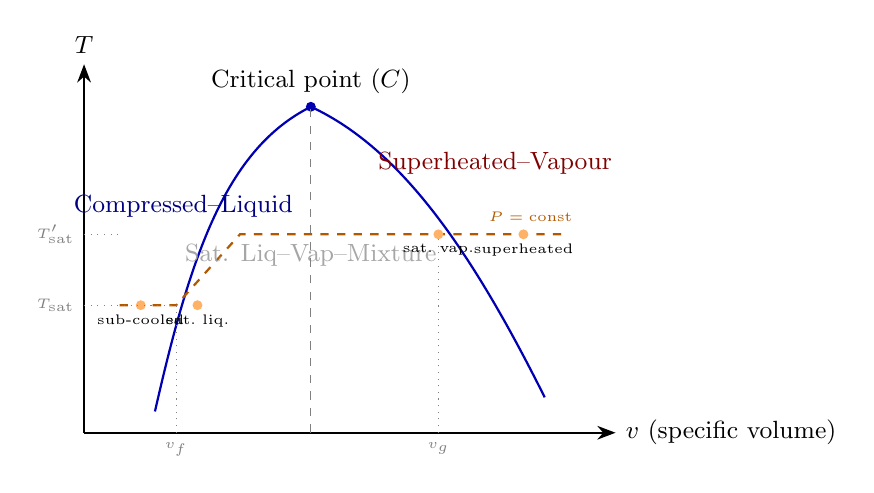
\begin{tikzpicture}[scale=0.90,arr/.style={-Stealth,thick}]
  \draw[arr](0,0)--(7.5,0) node[right,font=\small]{$v$ (specific volume)};
  \draw[arr](0,0)--(0,5.2) node[above,font=\small]{$T$};

  % Saturation dome
  \draw[thick,blue!70!black]
    (1.0,0.3)
    .. controls (1.5,2.5) and (2.0,4.0) .. (3.2,4.6)  % left (liquid) side
    .. controls (4.5,4.0) and (5.5,2.5) .. (6.5,0.5); % right (vapour) side
  \fill[blue!70!black] (3.2,4.6) circle(0.07);
  \node[font=\small,above] at (3.2,4.65) {Critical point ($C$)};

  % Isobar (constant pressure line)
  \draw[thick,orange!70!black,dashed]
    (0.5,1.8)--(1.3,1.8)--(2.2,2.8)--(6.8,2.8);
  \node[font=\tiny,orange!70!black,above] at (6.3,2.85) {$P=\text{const}$};

  % Region labels
  \node[font=\small,align=center,blue!50!black]   at (1.4,3.2)  {Compressed--Liquid};
  \node[font=\small,align=center,gray!70]   at (3.2,2.5)  {Sat. Liq--Vap--Mixture};
  \node[font=\small,align=center,red!50!black]    at (5.8,3.8)  {Superheated--Vapour};

  % Saturation lines
  \draw[dashed,gray] (3.2,0)--(3.2,4.6)
    node[below=4.2cm,font=\tiny,gray]{};
  \node[font=\tiny,gray,below] at (1.3,0) {$v_f$};
  \node[font=\tiny,gray,below] at (5.0,0) {$v_g$};
  \draw[dotted,gray](1.3,0)--(1.3,1.8);
  \draw[dotted,gray](5.0,0)--(5.0,2.8);

  % State labels on isobar
  \fill[orange!60] (0.8,1.8) circle(0.07);
  \node[font=\tiny,below] at (0.8,1.8) {sub-cooled};
  \fill[orange!60] (1.6,1.8) circle(0.07);
  \node[font=\tiny,below] at (1.6,1.8) {sat.\ liq.};
  \fill[orange!60] (5.0,2.8) circle(0.07);
  \node[font=\tiny,below] at (5.0,2.8) {sat.\ vap.};
  \fill[orange!60] (6.2,2.8) circle(0.07);
  \node[font=\tiny,below] at (6.2,2.8) {superheated};

  % Tsat label
  \draw[dotted,gray](0,1.8)node[left,font=\tiny]{$T_\text{sat}$}--(1.3,1.8);
  \draw[dotted,gray](0,2.8)node[left,font=\tiny]{$T_\text{sat}'$}--(0.5,2.8);

\end{tikzpicture}
\end{center}

\textbf{Regions:}
\begin{itemize}[leftmargin=1.5em,itemsep=1pt]
  \item \textbf{Left of dome:} Compressed (sub-cooled) liquid —
        $T < T_\text{sat}$ at given $P$.
  \item \textbf{Under the dome:} Saturated liquid--vapour mixture —
        two phases coexist.
  \item \textbf{Right of dome:} Superheated vapour —
        $T > T_\text{sat}$ at given $P$.
  \item \textbf{Apex of dome:} Critical point — above this, no phase
        distinction exists.
\end{itemize}

\end{tcolorbox}

\item \label{qlabel:A3-Q27}
(a) Define refrigeration. What is one ton of refrigeration? With T-s diagrams explain the difference between Reversed Carnot Cycle and Vapour Compression Cycle. \mk{14}\\
(b) Mention desirable properties of refrigerants. Write chemical formulas of R-134, R-22, R-718. \mk{6}\\
(c) A refrigerator uses R-134a between 0.14\,MPa and 0.9\,MPa. Mass flow rate\,$= 0.08$\,kg/s. Determine: (i) rate of heat removed, (ii) rate of heat rejection, (iii) power input, (iv) COP. \mk{15}
\yr{2015--16}


\noindent\textbf{\Large TABLE A--11} \\
\noindent\textbf{\large Properties of Saturated Refrigerant 134a (Liquid-Vapor): Pressure Table}
\vspace{0.3cm}

\begin{center}
\small
\begin{longtable}{c c c c c c c c c c c c}
\toprule\toprule
& & \multicolumn{2}{c}{\textit{Specific Volume}} & \multicolumn{2}{c}{\textit{Internal Energy}} & \multicolumn{3}{c}{\textit{Enthalpy}} & \multicolumn{2}{c}{\textit{Entropy}} & \\
& & \multicolumn{2}{c}{$\text{m}^3\text{/kg}$} & \multicolumn{2}{c}{$\text{kJ/kg}$} & \multicolumn{3}{c}{$\text{kJ/kg}$} & \multicolumn{2}{c}{$\text{kJ/kg}\cdot\text{K}$} & \\
\cmidrule(lr){3-4} \cmidrule(lr){5-6} \cmidrule(lr){7-9} \cmidrule(lr){10-11}
Press. & Temp. & Sat. Liquid & Sat. Vapor & Sat. Liquid & Sat. Vapor & Sat. Liquid & Evap. & Sat. Vapor & Sat. Liquid & Sat. Vapor & Press. \\
bar & $^\circ\text{C}$ & $v_f \times 10^3$ & $v_g$ & $u_f$ & $u_g$ & $h_f$ & $h_{fg}$ & $h_g$ & $s_f$ & $s_g$ & bar \\
\midrule
\endhead

\midrule
\multicolumn{12}{r}{{Continued on next page}} \\
\bottomrule
\endfoot

\bottomrule\bottomrule
\endlastfoot

0.6 & -37.07 & 0.7097 & 0.3100 & 3.41 & 206.12 & 3.46 & 221.27 & 224.72 & 0.0147 & 0.9520 & 0.6 \\
0.8 & -31.21 & 0.7184 & 0.2366 & 10.41 & 209.46 & 10.47 & 217.92 & 228.39 & 0.0440 & 0.9447 & 0.8 \\
1.0 & -26.43 & 0.7258 & 0.1917 & 16.22 & 212.18 & 16.29 & 215.06 & 231.35 & 0.0678 & 0.9395 & 1.0 \\
1.2 & -22.36 & 0.7323 & 0.1614 & 21.23 & 214.50 & 21.32 & 212.54 & 233.86 & 0.0879 & 0.9354 & 1.2 \\
1.4 & -18.80 & 0.7381 & 0.1395 & 25.66 & 216.52 & 25.77 & 210.27 & 236.04 & 0.1055 & 0.9322 & 1.4 \\
\addlinespace
1.6 & -15.62 & 0.7435 & 0.1229 & 29.66 & 218.32 & 29.78 & 208.19 & 237.97 & 0.1211 & 0.9295 & 1.6 \\
1.8 & -12.73 & 0.7485 & 0.1098 & 33.31 & 219.94 & 33.45 & 206.26 & 239.71 & 0.1352 & 0.9273 & 1.8 \\
2.0 & -10.09 & 0.7532 & 0.0993 & 36.69 & 221.43 & 36.84 & 204.46 & 241.30 & 0.1481 & 0.9253 & 2.0 \\
2.4 & -5.37 & 0.7618 & 0.0834 & 42.77 & 224.07 & 42.95 & 201.14 & 244.09 & 0.1710 & 0.9222 & 2.4 \\
2.8 & -1.23 & 0.7697 & 0.0719 & 48.18 & 226.38 & 48.39 & 198.13 & 246.52 & 0.1911 & 0.9197 & 2.8 \\
\addlinespace
3.2 & 2.48 & 0.7770 & 0.0632 & 53.06 & 228.43 & 53.31 & 195.35 & 248.66 & 0.2089 & 0.9177 & 3.2 \\
3.6 & 5.84 & 0.7839 & 0.0564 & 57.54 & 230.28 & 57.82 & 192.76 & 250.58 & 0.2251 & 0.9160 & 3.6 \\
4.0 & 8.93 & 0.7904 & 0.0509 & 61.69 & 231.97 & 62.00 & 190.32 & 252.32 & 0.2399 & 0.9145 & 4.0 \\
5.0 & 15.74 & 0.8056 & 0.0409 & 70.93 & 235.64 & 71.33 & 184.74 & 256.07 & 0.2723 & 0.9117 & 5.0 \\
6.0 & 21.58 & 0.8196 & 0.0341 & 78.99 & 238.74 & 79.48 & 179.71 & 259.19 & 0.2999 & 0.9097 & 6.0 \\
\addlinespace
7.0 & 26.72 & 0.8328 & 0.0292 & 86.19 & 241.42 & 86.78 & 175.07 & 261.85 & 0.3242 & 0.9080 & 7.0 \\
8.0 & 31.33 & 0.8454 & 0.0255 & 92.75 & 243.78 & 93.42 & 170.73 & 264.15 & 0.3459 & 0.9066 & 8.0 \\
9.0 & 35.53 & 0.8576 & 0.0226 & 98.79 & 245.88 & 99.56 & 166.62 & 266.18 & 0.3656 & 0.9054 & 9.0 \\
10.0 & 39.39 & 0.8695 & 0.0202 & 104.42 & 247.77 & 105.29 & 162.68 & 267.97 & 0.3838 & 0.9043 & 10.0 \\
12.0 & 46.32 & 0.8928 & 0.0166 & 114.69 & 251.03 & 115.76 & 155.23 & 270.99 & 0.4164 & 0.9023 & 12.0 \\
\addlinespace
14.0 & 52.43 & 0.9159 & 0.0140 & 123.98 & 253.74 & 125.26 & 148.14 & 273.40 & 0.4453 & 0.9003 & 14.0 \\
16.0 & 57.92 & 0.9392 & 0.0121 & 132.52 & 256.00 & 134.02 & 141.31 & 275.33 & 0.4714 & 0.8982 & 16.0 \\
18.0 & 62.91 & 0.9631 & 0.0105 & 140.49 & 257.88 & 142.22 & 134.60 & 276.83 & 0.4954 & 0.8959 & 18.0 \\
20.0 & 67.49 & 0.9878 & 0.0093 & 148.02 & 259.41 & 149.99 & 127.95 & 277.94 & 0.5178 & 0.8934 & 20.0 \\
25.0 & 77.59 & 1.0562 & 0.0069 & 165.48 & 261.84 & 168.12 & 111.06 & 279.17 & 0.5687 & 0.8854 & 25.0 \\
\addlinespace
30.0 & 86.22 & 1.1416 & 0.0053 & 181.88 & 262.16 & 185.30 & 92.71 & 278.01 & 0.6156 & 0.8735 & 30.0 \\
\end{longtable}
\end{center}

\vspace{0.1cm}
\noindent\footnotesize \textit{Note:} Pressure Conversions: 1 bar = 0.1 MPa = $10^2$ kPa. \\

\noindent\textbf{\Large TABLE A--13} \\
\noindent\textbf{\large Properties of Superheated Refrigerant 134a}
\vspace{0.3cm}

\begin{center}
\small
\begin{tabular}{r c c c c p{0.2cm} r c c c c}
\toprule\toprule
$T$ & $v$ & $u$ & $h$ & $s$ & & $T$ & $v$ & $u$ & $h$ & $s$ \\
$^\circ\text{C}$ & $\text{m}^3\text{/kg}$ & $\text{kJ/kg}$ & $\text{kJ/kg}$ & $\text{kJ/kg}\cdot\text{K}$ & & $^\circ\text{C}$ & $\text{m}^3\text{/kg}$ & $\text{kJ/kg}$ & $\text{kJ/kg}$ & $\text{kJ/kg}\cdot\text{K}$ \\
\midrule
\multicolumn{5}{c}{\textbf{p = 1.4 bar = 0.14 MPa} ($T_{\text{sat}} = -18.80^\circ\text{C}$)} & & \multicolumn{5}{c}{\textbf{p = 1.8 bar = 0.18 MPa} ($T_{\text{sat}} = -12.73^\circ\text{C}$)} \\
\cmidrule(lr){1-5} \cmidrule(lr){7-11}
Sat. & 0.13945 & 216.52 & 236.04 & 0.9322 & & Sat. & 0.10983 & 219.94 & 239.71 & 0.9273 \\
-10 & 0.14549 & 223.03 & 243.40 & 0.9606 & & -10 & 0.11135 & 222.02 & 242.06 & 0.9362 \\
0 & 0.15219 & 230.55 & 251.86 & 0.9922 & & 0 & 0.11678 & 229.67 & 250.69 & 0.9684 \\
10 & 0.15875 & 238.21 & 260.43 & 1.0230 & & 10 & 0.12207 & 237.44 & 259.41 & 0.9998 \\
20 & 0.16520 & 246.01 & 269.13 & 1.0532 & & 20 & 0.12723 & 245.33 & 268.23 & 1.0304 \\ \addlinespace
30 & 0.17155 & 253.96 & 277.97 & 1.0828 & & 30 & 0.13230 & 253.36 & 277.17 & 1.0604 \\
40 & 0.17783 & 262.06 & 286.96 & 1.1120 & & 40 & 0.13730 & 261.53 & 286.24 & 1.0898 \\
50 & 0.18404 & 270.32 & 296.09 & 1.1407 & & 50 & 0.14222 & 269.85 & 295.45 & 1.1187 \\
60 & 0.19020 & 278.74 & 305.37 & 1.1690 & & 60 & 0.14710 & 278.31 & 304.79 & 1.1472 \\
70 & 0.19633 & 287.32 & 314.80 & 1.1969 & & 70 & 0.15193 & 286.93 & 314.28 & 1.1753 \\ \addlinespace
80 & 0.20241 & 296.06 & 324.39 & 1.2244 & & 80 & 0.15672 & 295.71 & 323.92 & 1.2030 \\
90 & 0.20846 & 304.95 & 334.14 & 1.2516 & & 90 & 0.16148 & 304.63 & 333.70 & 1.2303 \\
100 & 0.21449 & 314.01 & 344.04 & 1.2785 & & 100 & 0.16622 & 313.72 & 343.63 & 1.2573 \\
\midrule[\lightrulewidth]
\multicolumn{5}{c}{\textbf{p = 8.0 bar = 0.80 MPa} ($T_{\text{sat}} = 31.33^\circ\text{C}$)} & & \multicolumn{5}{c}{\textbf{p = 9.0 bar = 0.90 MPa} ($T_{\text{sat}} = 35.53^\circ\text{C}$)} \\
\cmidrule(lr){1-5} \cmidrule(lr){7-11}
Sat. & 0.02547 & 243.78 & 264.15 & 0.9066 & & Sat. & 0.02255 & 245.88 & 266.18 & 0.9054 \\
40 & 0.02691 & 252.13 & 273.66 & 0.9374 & & 40 & 0.02325 & 250.32 & 271.25 & 0.9217 \\
50 & 0.02846 & 261.62 & 284.39 & 0.9711 & & 50 & 0.02472 & 260.09 & 282.34 & 0.9566 \\
60 & 0.02992 & 271.04 & 294.98 & 1.0034 & & 60 & 0.02609 & 269.72 & 293.21 & 0.9897 \\
70 & 0.03131 & 280.45 & 305.50 & 1.0345 & & 70 & 0.02738 & 279.30 & 303.94 & 1.0214 \\ \addlinespace
80 & 0.03264 & 289.89 & 316.00 & 1.0647 & & 80 & 0.02861 & 288.87 & 314.62 & 1.0521 \\
90 & 0.03393 & 299.37 & 326.52 & 1.0940 & & 90 & 0.02880 & 298.46 & 325.28 & 1.0819 \\
100 & 0.03519 & 308.93 & 337.08 & 1.1227 & & 100 & 0.03095 & 308.11 & 335.96 & 1.1109 \\
110 & 0.03642 & 318.57 & 347.71 & 1.1508 & & 110 & 0.03207 & 317.82 & 346.68 & 1.1392 \\
120 & 0.03762 & 328.31 & 358.40 & 1.1784 & & 120 & 0.03316 & 327.62 & 357.47 & 1.1670 \\ \addlinespace
130 & 0.03881 & 338.14 & 369.19 & 1.2055 & & 130 & 0.03423 & 337.52 & 368.33 & 1.1943 \\
140 & 0.03997 & 348.09 & 380.07 & 1.2321 & & 140 & 0.03529 & 347.51 & 379.27 & 1.2211 \\
150 & 0.04113 & 358.15 & 391.05 & 1.2584 & & 150 & 0.03633 & 357.61 & 390.31 & 1.2475 \\
160 & 0.04227 & 368.32 & 402.14 & 1.2843 & & 160 & 0.03736 & 367.82 & 401.44 & 1.2735 \\
170 & 0.04340 & 378.61 & 413.33 & 1.3098 & & 170 & 0.03838 & 378.14 & 412.68 & 1.2992 \\ \addlinespace
180 & 0.04452 & 389.02 & 424.63 & 1.3351 & & 180 & 0.03939 & 388.57 & 424.02 & 1.3245 \\
\midrule[\lightrulewidth]
\multicolumn{5}{c}{\textbf{p = 14.0 bar = 1.40 MPa} ($T_{\text{sat}} = 52.43^\circ\text{C}$)} & & \multicolumn{5}{c}{\textbf{p = 16.0 bar = 1.60 MPa} ($T_{\text{sat}} = 57.92^\circ\text{C}$)} \\
\cmidrule(lr){1-5} \cmidrule(lr){7-11}
Sat. & 0.01405 & 253.74 & 273.40 & 0.9003 & & Sat. & 0.01208 & 256.00 & 275.33 & 0.8982 \\
60 & 0.01495 & 262.17 & 283.10 & 0.9297 & & 60 & 0.01233 & 258.48 & 278.20 & 0.9069 \\
70 & 0.01603 & 272.87 & 295.31 & 0.9658 & & 70 & 0.01340 & 269.89 & 291.33 & 0.9457 \\
80 & 0.01701 & 283.29 & 307.10 & 0.9997 & & 80 & 0.01435 & 280.78 & 303.74 & 0.9813 \\
90 & 0.01792 & 293.55 & 318.63 & 1.0319 & & 90 & 0.01521 & 291.39 & 315.72 & 1.0148 \\ \addlinespace
100 & 0.01878 & 303.73 & 330.02 & 1.0628 & & 100 & 0.01601 & 301.84 & 327.46 & 1.0467 \\
110 & 0.01960 & 313.88 & 341.32 & 1.0927 & & 110 & 0.01677 & 312.20 & 339.04 & 1.0773 \\
120 & 0.02039 & 324.05 & 352.59 & 1.1218 & & 120 & 0.01750 & 322.53 & 350.53 & 1.1069 \\
130 & 0.02115 & 334.25 & 363.86 & 1.1501 & & 130 & 0.01820 & 332.87 & 361.99 & 1.1357 \\
140 & 0.02189 & 344.50 & 375.15 & 1.1777 & & 140 & 0.01887 & 343.24 & 373.44 & 1.1638 \\ \addlinespace
150 & 0.02262 & 354.82 & 386.49 & 1.2048 & & 150 & 0.01953 & 353.66 & 384.91 & 1.1912 \\
160 & 0.02333 & 365.22 & 397.89 & 1.2315 & & 160 & 0.02017 & 364.15 & 396.43 & 1.2181 \\
170 & 0.02403 & 375.71 & 409.36 & 1.2576 & & 170 & 0.02080 & 374.71 & 407.99 & 1.2445 \\
180 & 0.02472 & 386.29 & 420.90 & 1.2843 & & 180 & 0.02142 & 385.35 & 419.62 & 1.2704 \\
190 & 0.02541 & 396.96 & 432.53 & 1.3088 & & 190 & 0.02203 & 396.08 & 431.33 & 1.2960 \\ \addlinespace
200 & 0.02608 & 407.73 & 444.24 & 1.3338 & & 200 & 0.02263 & 406.90 & 443.11 & 1.3212 \\
\bottomrule\bottomrule
\end{tabular}
\end{center}

\begin{tcolorbox}[enhanced,breakable,ansbox,colback=cC!4,colframe=cC,
  boxrule=0.8pt,arc=5pt,
  title={\textbf{Solution}},fonttitle=\bfseries\color{white},colbacktitle=cC]


\textbf{Part (a): Refrigeration, Ton of Refrigeration, and T-s Diagrams}

\textbf{Refrigeration:} The process of removing heat from an enclosed space
or substance to lower its temperature and maintain it below the ambient
temperature. A refrigeration system achieves this by absorbing heat at a
low temperature (evaporator) and rejecting it at a higher temperature
(condenser), requiring work input.

\textbf{One Ton of Refrigeration:} \variant{A3-Q4(a) — derivation given there}
$1\,\text{TR} \approx 3.517\,\text{kW}$.

\textbf{Reversed Carnot Cycle vs.\ Vapour Compression Cycle (T-s diagrams):}

\begin{center}
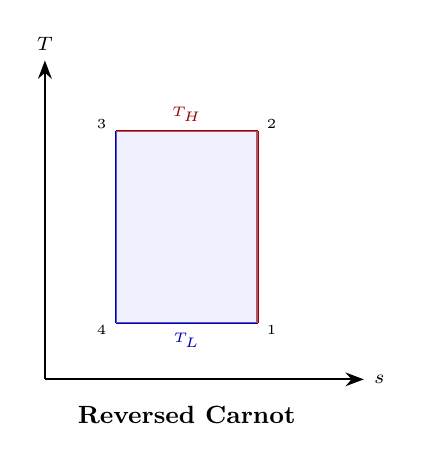
\begin{tikzpicture}[scale=0.90,arr/.style={-Stealth,thick}]

  %% Reversed Carnot
  \begin{scope}[xshift=0cm]
    \draw[arr](0,0)--(4.5,0) node[right,font=\scriptsize]{$s$};
    \draw[arr](0,0)--(0,4.5) node[above,font=\scriptsize]{$T$};
    % Rectangle
    \draw[thick,blue!70!black] (1.0,0.8)--(3.0,0.8) % 4-1 isothermal absorption
      node[midway,below,font=\tiny]{$T_L$};
    \draw[thick,red!60!black]  (3.0,0.8)--(3.0,3.5) % 1-2 isentropic compression
      node[right,font=\tiny]{};
    \draw[thick,red!60!black]  (3.0,3.5)--(1.0,3.5) % 2-3 isothermal rejection
      node[midway,above,font=\tiny]{$T_H$};
    \draw[thick,blue!70!black] (1.0,3.5)--(1.0,0.8) % 3-4 isentropic expansion
      node[left,font=\tiny]{};
    % labels
    \node[font=\tiny] at (3.2,3.6) {2};
    \node[font=\tiny] at (3.2,0.7) {1};
    \node[font=\tiny] at (0.8,0.7) {4};
    \node[font=\tiny] at (0.8,3.6) {3};
    \node[font=\small\bfseries] at (2.0,-0.5) {Reversed Carnot};
    \fill[blue!15,opacity=0.4]  (1.0,0.8) rectangle (3.0,3.5);
  \end{scope}

\end{tikzpicture}
  
\includegraphics[height=0.3\textheight,width=0.75\textwidth,keepaspectratio]{/T-s.png}

\end{center}

\textbf{Key differences:}
\begin{itemize}[leftmargin=1.5em,itemsep=1pt]
  \item In the Carnot cycle, \emph{all} processes are ideal (two isothermals +
        two isentropics) — a rectangle on the T-s diagram. It gives the maximum
        possible COP.
  \item In the VCR cycle, the isentropic \emph{expansion} is replaced by an
        \textbf{isenthalpic throttling} (irreversible) — this causes loss of
        work and a lower COP than Carnot.
  \item The VCR cycle operates partly outside the saturation dome (superheated
        compression), whereas Carnot would require wet compression.
  \item VCR is practically realisable; Carnot is an ideal reference.
\end{itemize}

\hrulefill

\textbf{Part (b): Refrigerant Properties and Formulas}

\textit{Desirable properties:} \variant{A3-Q (b) — full list given earlier}

\begin{center}
\small
\begin{tabular}{@{}llll@{}}
\toprule
\textbf{Refrigerant} & \textbf{Chemical Name} & \textbf{Formula} & \textbf{Note} \\
\midrule
R-134a & 1,1,1,2-Tetrafluoroethane & CH$_2$FCF$_3$ & HFC; ODP\,=\,0 \\
R-22   & Chlorodifluoromethane     & CHClF$_2$     & HCFC; being phased out \\
R-718  & Water                     & H$_2$O        & Used in absorption systems \\
\bottomrule
\end{tabular}
\end{center}


\medskip
\textbf{Part (a):}

\textbf{Given:} R-134a,\;
$P_\text{low} = 0.14$\,MPa,\;
$P_\text{high} = 0.90$\,MPa,\;
$\dot{m} = 0.08$\,kg/s.

\medskip
\textbf{State 1} --- saturated vapour at $P = 140$\,kPa (Table A-11):
\[
  h_1 = 239.16\,\text{kJ/kg}, \qquad s_1 = 0.9447\,\text{kJ/kg\,K}
\]

\textbf{State 3} --- saturated liquid at $P = 900$\,kPa (Table A-11):
\[
  h_3 = 101.61\,\text{kJ/kg}
\]

\textbf{State 4} --- evaporator inlet (isenthalpic throttling):
\[
  h_4 = h_3 = 101.61\,\text{kJ/kg}
\]

\textbf{State 2} --- superheated vapour at $P = 0.90$\,MPa,
$s_2 = s_1 = 0.9447$\,kJ/kg\,K.
Interpolating between $40^\circ$C and $50^\circ$C (Table A-13):
\[
  x = \frac{0.9447 - 0.9327}{0.9666 - 0.9327}
    = \frac{0.0120}{0.0339} \approx 0.354
\]
\[
  h_2 = 274.15 + 0.354\times(285.34 - 274.15)
      = 274.15 + 3.96
      = 278.11\,\text{kJ/kg}
\]

\medskip
\textbf{(i) Rate of heat removal:}
\[
  \dot{Q}_L = \dot{m}(h_1 - h_4)
  = 0.08\times(239.16 - 101.61)
  \quad\boxed{\dot{Q}_L = 11.004\,\text{kW}}
\]

\textbf{(ii) Rate of heat rejection:}
\[
  \dot{Q}_H = \dot{m}(h_2 - h_3)
  = 0.08\times(278.11 - 101.61)
  \quad\boxed{\dot{Q}_H = 14.12\,\text{kW}}
\]

\textbf{(iii) Power input:}
\[
  \dot{W}_\text{in} = \dot{m}(h_2 - h_1)
  = 0.08\times(278.11 - 239.16)
  \quad\boxed{\dot{W}_\text{in} = 3.116\,\text{kW}}
\]

\textbf{(iv) COP:}
\[
  \mathrm{COP} = \frac{\dot{Q}_L}{\dot{W}_\text{in}}
  = \frac{11.004}{3.116}
  \quad\boxed{\mathrm{COP} \approx 3.53}
\]

\end{tcolorbox}

\item \label{qlabel:A3-Q28}
Air at 35\textdegree C DBT and 60\% RH at 2\,kg/s mixed with air at 4\,kg/s, 20\textdegree C WBT and 30\textdegree C DBT. Calculate for final mixture: (i) Absolute humidity, (ii) RH, (iii) DBT and WBT, (iv) Dew point, (v) Enthalpy. \mk{15}
\yr{2015--16} \variant{A3-Q12, A3-Q17 identical numerical}


\begin{center}
  
\includegraphics[height=0.3\textheight,width=0.85\textwidth,height=0.3\textheight,keepaspectratio]{/29.png}
\end{center}

\item \label{qlabel:A3-Q25}
(a) Write chemical formula of any three: R717, R12, R112, R290. \mk{6}\\
(b) Draw schematic and T-s diagram of vapour compression refrigeration with multistage compression. \mk{14}\\
(c) A refrigerator: COP\,$= 4.0$, compressor work\,$= 0.5$\,kW, mass flow rate\,$= 0.05$\,kg/s. Determine: (i) rate of heat removal, (ii) rate of heat rejection, (iii) COP as heat pump. \mk{9}\\
(d) Define: (i) tonne of refrigeration (TR), (ii) COP. \mk{6}
\yr{2014--15}


\item \label{qlabel:A3-Q26}
2\,kg air at 40\textdegree C DBT and 50\% RH mixed with 1\,kg air at 22\textdegree C DBT and 17\textdegree C WBT. Calculate: (i) temperature, (ii) dew point temperature, (iii) specific humidity, (iv) relative humidity of mixture. \mk{25}
\yr{2014--15}


\begin{center}
  
\includegraphics[height=0.3\textheight,width=0.85\textwidth,height=0.3\textheight,keepaspectratio]{/100.png}
\end{center}

\item \label{qlabel:A3-Q23}
(a) Briefly write down desirable properties of a good refrigerant. \mk{6}\\
(b) Briefly explain vapour absorption refrigeration cycle with necessary schematic diagram. \mk{14}\\
(c) A refrigerator uses R-134a between 0.18 and 0.9\,MPa. Mass flow rate\,$= 0.07$\,kg/s. Determine: (i) rate of heat removal, (ii) power input, (iii) COP, (iv) COP if used as heat pump. \mk{15}
\yr{2013--14}


\noindent\textbf{\Large TABLE A--12} \\
\noindent\textbf{\large Saturated refrigerant-134a---Pressure table}
\vspace{0.3cm}

\begin{center}
\small
\begin{longtable}{c c c c c c c c c c c c c}
\toprule\toprule
& & \multicolumn{2}{c}{\textit{Specific volume,}} & \multicolumn{3}{c}{\textit{Internal energy,}} & \multicolumn{3}{c}{\textit{Enthalpy,}} & \multicolumn{3}{c}{\textit{Entropy,}} \\
& & \multicolumn{2}{c}{$\text{m}^3\text{/kg}$} & \multicolumn{3}{c}{$\text{kJ/kg}$} & \multicolumn{3}{c}{$\text{kJ/kg}$} & \multicolumn{3}{c}{$\text{kJ/kg}\cdot\text{K}$} \\
\cmidrule(lr){3-4} \cmidrule(lr){5-7} \cmidrule(lr){8-10} \cmidrule(lr){11-13}
& Sat. & Sat. & Sat. & Sat. & & Sat. & Sat. & & Sat. & Sat. & & Sat. \\
Press., & temp., & liquid, & vapor, & liquid, & Evap., & vapor, & liquid, & Evap., & vapor, & liquid, & Evap., & vapor, \\
$P$ kPa & $T_{\text{sat}}$ $^\circ\text{C}$ & $v_f$ & $v_g$ & $u_f$ & $u_{fg}$ & $u_g$ & $h_f$ & $h_{fg}$ & $h_g$ & $s_f$ & $s_{fg}$ & $s_g$ \\
\midrule
\endhead

\midrule
\multicolumn{13}{r}{{Continued on next page}} \\
\bottomrule
\endfoot

\bottomrule\bottomrule
\endlastfoot

60 & -36.95 & 0.0007098 & 0.31121 & 3.798 & 205.32 & 209.12 & 3.841 & 223.95 & 227.79 & 0.01634 & 0.94807 & 0.96441 \\
70 & -33.87 & 0.0007144 & 0.26929 & 7.680 & 203.20 & 210.88 & 7.730 & 222.00 & 229.73 & 0.03267 & 0.92775 & 0.96042 \\
80 & -31.13 & 0.0007185 & 0.23753 & 11.15 & 201.30 & 212.46 & 11.21 & 220.25 & 231.46 & 0.04711 & 0.90999 & 0.95710 \\
90 & -28.65 & 0.0007223 & 0.21263 & 14.31 & 199.57 & 213.88 & 14.37 & 218.65 & 233.02 & 0.06008 & 0.89419 & 0.95427 \\
100 & -26.37 & 0.0007259 & 0.19254 & 17.21 & 197.98 & 215.19 & 17.28 & 217.16 & 234.44 & 0.07188 & 0.87995 & 0.95183 \\
\addlinespace
120 & -22.32 & 0.0007324 & 0.16212 & 22.40 & 195.11 & 217.51 & 22.49 & 214.48 & 236.97 & 0.09275 & 0.85503 & 0.94779 \\
140 & -18.77 & 0.0007383 & 0.14014 & 26.98 & 192.57 & 219.54 & 27.08 & 212.08 & 239.16 & 0.11087 & 0.83368 & 0.94456 \\
160 & -15.60 & 0.0007437 & 0.12348 & 31.09 & 190.27 & 221.35 & 31.21 & 209.90 & 241.11 & 0.12693 & 0.81496 & 0.94190 \\
180 & -12.73 & 0.0007487 & 0.11041 & 34.83 & 188.16 & 222.99 & 34.97 & 207.90 & 242.86 & 0.14139 & 0.79826 & 0.93965 \\
200 & -10.09 & 0.0007533 & 0.099867 & 38.28 & 186.21 & 224.48 & 38.43 & 206.03 & 244.46 & 0.15457 & 0.78316 & 0.93773 \\
\addlinespace
240 & -5.38 & 0.0007620 & 0.083897 & 44.48 & 182.67 & 227.14 & 44.66 & 202.62 & 247.28 & 0.17794 & 0.75664 & 0.93458 \\
280 & -1.25 & 0.0007699 & 0.072352 & 49.97 & 179.50 & 229.46 & 50.18 & 199.54 & 249.72 & 0.19829 & 0.73381 & 0.93210 \\
320 & 2.46 & 0.0007772 & 0.063604 & 54.92 & 176.61 & 231.52 & 55.16 & 196.71 & 251.88 & 0.21637 & 0.71369 & 0.93006 \\
360 & 5.82 & 0.0007841 & 0.056738 & 59.44 & 173.94 & 233.38 & 59.72 & 194.08 & 253.81 & 0.23270 & 0.69566 & 0.92836 \\
400 & 8.91 & 0.0007907 & 0.051201 & 63.62 & 171.45 & 235.07 & 63.94 & 191.62 & 255.55 & 0.24761 & 0.67929 & 0.92691 \\
\addlinespace
450 & 12.46 & 0.0007985 & 0.045619 & 68.45 & 168.54 & 237.00 & 68.81 & 188.71 & 257.53 & 0.26465 & 0.66069 & 0.92535 \\
500 & 15.71 & 0.0008059 & 0.041118 & 72.93 & 165.82 & 238.75 & 73.33 & 185.98 & 259.30 & 0.28023 & 0.64377 & 0.92400 \\
550 & 18.73 & 0.0008130 & 0.037408 & 77.10 & 163.25 & 240.35 & 77.54 & 183.38 & 260.92 & 0.29461 & 0.62821 & 0.92282 \\
600 & 21.55 & 0.0008199 & 0.034295 & 81.02 & 160.81 & 241.83 & 81.51 & 180.90 & 262.40 & 0.30799 & 0.61378 & 0.92177 \\
650 & 24.20 & 0.0008266 & 0.031646 & 84.72 & 158.48 & 243.20 & 85.26 & 178.51 & 263.77 & 0.32051 & 0.60030 & 0.92081 \\
\addlinespace
700 & 26.69 & 0.0008331 & 0.029361 & 88.24 & 156.24 & 244.48 & 88.82 & 176.21 & 265.03 & 0.33230 & 0.58763 & 0.91994 \\
750 & 29.06 & 0.0008395 & 0.027371 & 91.59 & 154.08 & 245.67 & 92.22 & 173.98 & 266.20 & 0.34345 & 0.57567 & 0.91912 \\
800 & 31.31 & 0.0008458 & 0.025621 & 94.79 & 152.00 & 246.79 & 95.47 & 171.82 & 267.29 & 0.35404 & 0.56431 & 0.91835 \\
850 & 33.45 & 0.0008520 & 0.024069 & 97.87 & 149.98 & 247.85 & 98.60 & 169.71 & 268.31 & 0.36413 & 0.55349 & 0.91762 \\
\addlinespace
900 & 35.51 & 0.0008580 & 0.022683 & 100.83 & 148.01 & 248.85 & 101.61 & 167.66 & 269.26 & 0.37377 & 0.54315 & 0.91692 \\
950 & 37.48 & 0.0008641 & 0.021438 & 103.69 & 146.10 & 249.79 & 104.51 & 165.64 & 270.15 & 0.38301 & 0.53323 & 0.91624 \\
1000 & 39.37 & 0.0008700 & 0.020313 & 106.45 & 144.23 & 250.68 & 107.32 & 163.67 & 270.99 & 0.39189 & 0.52368 & 0.91558 \\
1200 & 46.29 & 0.0008934 & 0.016715 & 116.70 & 137.11 & 253.81 & 117.77 & 156.10 & 273.87 & 0.42441 & 0.48863 & 0.91303 \\
1400 & 52.40 & 0.0009166 & 0.014107 & 125.94 & 130.43 & 256.37 & 127.22 & 148.90 & 276.12 & 0.45315 & 0.45734 & 0.91050 \\
\addlinespace
1600 & 57.88 & 0.0009400 & 0.012123 & 134.43 & 124.04 & 258.47 & 135.93 & 141.93 & 277.86 & 0.47911 & 0.42873 & 0.90784 \\
1800 & 62.87 & 0.0009639 & 0.010559 & 142.33 & 117.83 & 260.17 & 144.07 & 135.11 & 279.17 & 0.50294 & 0.40204 & 0.90498 \\
2000 & 67.45 & 0.0009886 & 0.009288 & 149.78 & 111.73 & 261.51 & 151.76 & 128.33 & 280.09 & 0.52509 & 0.37675 & 0.90184 \\
2500 & 77.54 & 0.0010566 & 0.006936 & 166.99 & 96.47 & 263.45 & 169.63 & 111.16 & 280.79 & 0.57531 & 0.31695 & 0.89226 \\
3000 & 86.16 & 0.0011406 & 0.005275 & 183.04 & 80.22 & 263.26 & 186.46 & 92.63 & 279.09 & 0.62118 & 0.25776 & 0.87894 \\
\end{longtable}
\end{center}

\noindent\textbf{\Large TABLE A--13} \\
\noindent\textbf{\large Superheated refrigerant-134a}
\vspace{0.3cm}

\begin{center}
\small
\begin{longtable}{@{} c *{3}{@{\hspace{12pt}} c c c c} @{}}
\toprule\toprule
$T$ & $v$ & $u$ & $h$ & $s$ & $v$ & $u$ & $h$ & $s$ & $v$ & $u$ & $h$ & $s$ \\
$^\circ\text{C}$ & $\text{m}^3\text{/kg}$ & $\text{kJ/kg}$ & $\text{kJ/kg}$ & $\text{kJ/kg}\cdot\text{K}$ & $\text{m}^3\text{/kg}$ & $\text{kJ/kg}$ & $\text{kJ/kg}$ & $\text{kJ/kg}\cdot\text{K}$ & $\text{m}^3\text{/kg}$ & $\text{kJ/kg}$ & $\text{kJ/kg}$ & $\text{kJ/kg}\cdot\text{K}$ \\
\midrule
\endhead

\midrule
\multicolumn{13}{r}{{Continued on next page}} \\
\bottomrule
\endfoot

\bottomrule\bottomrule
\endlastfoot

% ----------------- BLOCK 4 -----------------
& \multicolumn{4}{c}{\textit{$P = 0.50$ MPa ($T_{\text{sat}} = 15.71^\circ\text{C}$)}} 
& \multicolumn{4}{c}{\textit{$P = 0.60$ MPa ($T_{\text{sat}} = 21.55^\circ\text{C}$)}} 
& \multicolumn{4}{c}{\textit{$P = 0.70$ MPa ($T_{\text{sat}} = 26.69^\circ\text{C}$)}} \\
\cmidrule(lr){2-5} \cmidrule(lr){6-9} \cmidrule(lr){10-13}
Sat. & 0.041118 & 238.75 & 259.30 & 0.9240 & 0.034295 & 241.83 & 262.40 & 0.9218 & 0.029361 & 244.48 & 265.03 & 0.9199 \\
20   & 0.042115 & 242.40 & 263.46 & 0.9383 & & & & & & & & \\
30   & 0.044338 & 250.84 & 273.01 & 0.9703 & 0.035984 & 249.22 & 270.81 & 0.9499 & 0.029966 & 247.48 & 268.45 & 0.9313 \\
40   & 0.046456 & 259.26 & 282.48 & 1.0011 & 0.037865 & 257.86 & 280.58 & 0.9816 & 0.031696 & 256.39 & 278.57 & 0.9641 \\
50   & 0.048499 & 267.72 & 291.96 & 1.0309 & 0.039659 & 266.48 & 290.28 & 1.0121 & 0.033322 & 265.20 & 288.53 & 0.9954 \\
60   & 0.050485 & 276.25 & 301.50 & 1.0599 & 0.041389 & 275.15 & 299.98 & 1.0417 & 0.034875 & 274.01 & 298.42 & 1.0256 \\
70   & 0.052427 & 284.89 & 311.10 & 1.0883 & 0.043069 & 283.89 & 309.73 & 1.0705 & 0.036373 & 282.87 & 308.33 & 1.0549 \\
80   & 0.054331 & 293.64 & 320.80 & 1.1162 & 0.044710 & 292.73 & 319.55 & 1.0987 & 0.037829 & 291.80 & 318.28 & 1.0835 \\
90   & 0.056205 & 302.51 & 330.61 & 1.1436 & 0.046318 & 301.67 & 329.46 & 1.1264 & 0.039250 & 300.82 & 328.29 & 1.1114 \\
100  & 0.058053 & 311.50 & 340.53 & 1.1705 & 0.047900 & 310.73 & 339.47 & 1.1536 & 0.040642 & 309.95 & 338.40 & 1.1389 \\
110  & 0.059880 & 320.63 & 350.57 & 1.1971 & 0.049458 & 319.91 & 349.59 & 1.1803 & 0.042010 & 319.19 & 348.60 & 1.1658 \\
120  & 0.061687 & 329.89 & 360.73 & 1.2233 & 0.050997 & 329.23 & 359.82 & 1.2067 & 0.043358 & 328.55 & 358.90 & 1.1924 \\
130  & 0.063479 & 339.29 & 371.03 & 1.2491 & 0.052519 & 338.67 & 370.18 & 1.2327 & 0.044688 & 338.04 & 369.32 & 1.2186 \\
140  & 0.065256 & 348.83 & 381.46 & 1.2747 & 0.054027 & 348.25 & 380.66 & 1.2584 & 0.046004 & 347.66 & 379.86 & 1.2444 \\
150  & 0.067021 & 358.51 & 392.02 & 1.2999 & 0.055522 & 357.96 & 391.27 & 1.2838 & 0.047306 & 357.41 & 390.52 & 1.2699 \\
160  & 0.068775 & 368.33 & 402.72 & 1.3249 & 0.057006 & 367.81 & 402.01 & 1.3088 & 0.048597 & 367.29 & 401.31 & 1.2951 \\
\midrule

% ----------------- BLOCK 5 -----------------
& \multicolumn{4}{c}{\textit{$P = 0.80$ MPa ($T_{\text{sat}} = 31.31^\circ\text{C}$)}} 
& \multicolumn{4}{c}{\textit{$P = 0.90$ MPa ($T_{\text{sat}} = 35.51^\circ\text{C}$)}} 
& \multicolumn{4}{c}{\textit{$P = 1.00$ MPa ($T_{\text{sat}} = 39.37^\circ\text{C}$)}} \\
\cmidrule(lr){2-5} \cmidrule(lr){6-9} \cmidrule(lr){10-13}
Sat. & 0.025621 & 246.79 & 267.29 & 0.9183 & 0.022683 & 248.85 & 269.26 & 0.9169 & 0.020313 & 250.68 & 270.99 & 0.9156 \\
40   & 0.027035 & 254.82 & 276.45 & 0.9480 & 0.023375 & 253.13 & 274.17 & 0.9327 & 0.020406 & 251.30 & 271.71 & 0.9179 \\
50   & 0.028547 & 263.86 & 286.69 & 0.9802 & 0.024809 & 262.44 & 284.77 & 0.9660 & 0.021796 & 260.94 & 282.74 & 0.9525 \\
60   & 0.029973 & 272.83 & 296.81 & 1.0110 & 0.026146 & 271.60 & 295.13 & 0.9976 & 0.023068 & 270.32 & 293.38 & 0.9850 \\
70   & 0.031340 & 281.81 & 306.88 & 1.0408 & 0.027413 & 280.72 & 305.39 & 1.0280 & 0.024261 & 279.59 & 303.85 & 1.0160 \\
80   & 0.032659 & 290.84 & 316.97 & 1.0698 & 0.028630 & 289.86 & 315.63 & 1.0574 & 0.025398 & 288.86 & 314.25 & 1.0458 \\
90   & 0.033941 & 299.95 & 327.10 & 1.0981 & 0.029806 & 299.06 & 325.89 & 1.0860 & 0.026492 & 298.15 & 324.64 & 1.0748 \\
100  & 0.035193 & 309.15 & 337.30 & 1.1258 & 0.030951 & 308.34 & 336.19 & 1.1140 & 0.027552 & 307.51 & 335.06 & 1.1031 \\
110  & 0.036420 & 318.45 & 347.59 & 1.1530 & 0.032068 & 317.70 & 346.56 & 1.1414 & 0.028584 & 316.94 & 345.53 & 1.1308 \\
120  & 0.037625 & 327.87 & 357.97 & 1.1798 & 0.033164 & 327.18 & 357.02 & 1.1684 & 0.029592 & 326.47 & 356.06 & 1.1580 \\
130  & 0.038813 & 337.40 & 368.45 & 1.2061 & 0.034241 & 336.76 & 367.58 & 1.1949 & 0.030581 & 336.11 & 366.69 & 1.1846 \\
140  & 0.039985 & 347.06 & 379.05 & 1.2321 & 0.035302 & 346.46 & 378.23 & 1.2210 & 0.031554 & 345.85 & 377.40 & 1.2109 \\
150  & 0.041143 & 356.85 & 389.76 & 1.2577 & 0.036349 & 356.28 & 389.00 & 1.2467 & 0.032512 & 355.71 & 388.22 & 1.2368 \\
160  & 0.042290 & 366.76 & 400.59 & 1.2830 & 0.037384 & 366.23 & 399.88 & 1.2721 & 0.033457 & 365.70 & 399.15 & 1.2623 \\
170  & 0.043427 & 376.81 & 411.55 & 1.3080 & 0.038408 & 376.31 & 410.88 & 1.2972 & 0.034392 & 375.81 & 410.20 & 1.2875 \\
180  & 0.044554 & 386.99 & 422.64 & 1.3327 & 0.039423 & 386.52 & 422.00 & 1.3221 & 0.035317 & 386.04 & 421.36 & 1.3124 \\
\midrule

% ----------------- BLOCK 6 -----------------
& \multicolumn{4}{c}{\textit{$P = 1.20$ MPa ($T_{\text{sat}} = 46.29^\circ\text{C}$)}} 
& \multicolumn{4}{c}{\textit{$P = 1.40$ MPa ($T_{\text{sat}} = 52.40^\circ\text{C}$)}} 
& \multicolumn{4}{c}{\textit{$P = 1.60$ MPa ($T_{\text{sat}} = 57.88^\circ\text{C}$)}} \\
\cmidrule(lr){2-5} \cmidrule(lr){6-9} \cmidrule(lr){10-13}
Sat. & 0.016715 & 253.81 & 273.87 & 0.9130 & 0.014107 & 256.37 & 276.12 & 0.9105 & 0.012123 & 258.47 & 277.86 & 0.9078 \\
50   & 0.017201 & 257.63 & 278.27 & 0.9267 & & & & & & & & \\
60   & 0.018404 & 267.56 & 289.64 & 0.9614 & 0.015005 & 264.46 & 285.47 & 0.9389 & 0.012372 & 260.89 & 280.69 & 0.9163 \\
70   & 0.019502 & 277.21 & 300.61 & 0.9938 & 0.016060 & 274.62 & 297.10 & 0.9733 & 0.013430 & 271.76 & 293.25 & 0.9535 \\
80   & 0.020529 & 286.75 & 311.39 & 1.0248 & 0.017023 & 284.51 & 308.34 & 1.0056 & 0.014362 & 282.09 & 305.07 & 0.9875 \\
90   & 0.021506 & 296.26 & 322.07 & 1.0546 & 0.017923 & 294.28 & 319.37 & 1.0364 & 0.015215 & 292.17 & 316.52 & 1.0194 \\
100  & 0.022442 & 305.80 & 332.73 & 1.0836 & 0.018778 & 304.01 & 330.30 & 1.0661 & 0.016014 & 302.14 & 327.76 & 1.0500 \\
110  & 0.023348 & 315.38 & 343.40 & 1.1118 & 0.019597 & 313.76 & 341.19 & 1.0949 & 0.016773 & 312.07 & 338.91 & 1.0795 \\
120  & 0.024228 & 325.03 & 354.11 & 1.1394 & 0.020388 & 323.55 & 352.09 & 1.1230 & 0.017500 & 322.02 & 350.02 & 1.1081 \\
130  & 0.025086 & 334.77 & 364.88 & 1.1664 & 0.021155 & 333.41 & 363.02 & 1.1504 & 0.018201 & 332.00 & 361.12 & 1.1360 \\
140  & 0.025927 & 344.61 & 375.72 & 1.1930 & 0.021904 & 343.34 & 374.01 & 1.1773 & 0.018882 & 342.05 & 372.26 & 1.1632 \\
150  & 0.026753 & 354.56 & 386.66 & 1.2192 & 0.022636 & 353.37 & 385.07 & 1.2038 & 0.019545 & 352.17 & 383.44 & 1.1900 \\
160  & 0.027566 & 364.61 & 397.69 & 1.2449 & 0.023355 & 363.51 & 396.20 & 1.2298 & 0.020194 & 362.38 & 394.69 & 1.2163 \\
170  & 0.028367 & 374.78 & 408.82 & 1.2703 & 0.024061 & 373.75 & 407.43 & 1.2554 & 0.020830 & 372.69 & 406.02 & 1.2421 \\
180  & 0.029158 & 385.08 & 420.07 & 1.2954 & 0.024757 & 384.10 & 418.76 & 1.2807 & 0.021456 & 383.11 & 417.44 & 1.2676 \\

\end{longtable}
\end{center}

\noindent\textbf{\Large TABLE A--17} \\
\noindent Ideal-gas properties of air
\vspace{0.3cm}

\begin{center}
\footnotesize
\begin{longtable}{cccccc|cccccc}
\toprule\toprule
$T$ & $h$ & & $u$ & & $s^\circ$ & $T$ & $h$ & & $u$ & & $s^\circ$ \\
K & kJ/kg & $P_r$ & kJ/kg & $v_r$ & kJ/kg$\cdot$K & K & kJ/kg & $P_r$ & kJ/kg & $v_r$ & kJ/kg$\cdot$K \\
\midrule
\endhead

\midrule
\multicolumn{12}{r}{{Continued on next page}} \\
\bottomrule
\endfoot

\bottomrule\bottomrule
\endlastfoot

200 & 199.97 & 0.3363 & 142.56 & 1707.0 & 1.29559 & 580 & 586.04 & 14.38 & 419.55 & 115.7 & 2.37348 \\
210 & 209.97 & 0.3987 & 149.69 & 1512.0 & 1.34444 & 590 & 596.52 & 15.31 & 427.15 & 110.6 & 2.39140 \\
220 & 219.97 & 0.4690 & 156.82 & 1346.0 & 1.39105 & 600 & 607.02 & 16.28 & 434.78 & 105.8 & 2.40902 \\
230 & 230.02 & 0.5477 & 164.00 & 1205.0 & 1.43557 & 610 & 617.53 & 17.30 & 442.42 & 101.2 & 2.42644 \\
240 & 240.02 & 0.6355 & 171.13 & 1084.0 & 1.47824 & 620 & 628.07 & 18.36 & 450.09 & 96.92 & 2.44356 \\
\addlinespace
250 & 250.05 & 0.7329 & 178.28 & 979.0 & 1.51917 & 630 & 638.63 & 19.84 & 457.78 & 92.84 & 2.46048 \\
260 & 260.09 & 0.8405 & 185.45 & 887.8 & 1.55848 & 640 & 649.22 & 20.64 & 465.50 & 88.99 & 2.47716 \\
270 & 270.11 & 0.9590 & 192.60 & 808.0 & 1.59634 & 650 & 659.84 & 21.86 & 473.25 & 85.34 & 2.49364 \\
280 & 280.13 & 1.0889 & 199.75 & 738.0 & 1.63279 & 660 & 670.47 & 23.13 & 481.01 & 81.89 & 2.50985 \\
285 & 285.14 & 1.1584 & 203.33 & 706.1 & 1.65055 & 670 & 681.14 & 24.46 & 488.81 & 78.61 & 2.52589 \\
\addlinespace
290 & 290.16 & 1.2311 & 206.91 & 676.1 & 1.66802 & 680 & 691.82 & 25.85 & 496.62 & 75.50 & 2.54175 \\
295 & 295.17 & 1.3068 & 210.49 & 647.9 & 1.68515 & 690 & 702.52 & 27.29 & 504.45 & 72.56 & 2.55731 \\
298 & 298.18 & 1.3543 & 212.64 & 631.9 & 1.69528 & 700 & 713.27 & 28.80 & 512.33 & 69.76 & 2.57277 \\
300 & 300.19 & 1.3860 & 214.07 & 621.2 & 1.70203 & 710 & 724.04 & 30.38 & 520.23 & 67.07 & 2.58810 \\
305 & 305.22 & 1.4686 & 217.67 & 596.0 & 1.71865 & 720 & 734.82 & 32.02 & 528.14 & 64.53 & 2.60319 \\
\addlinespace
310 & 310.24 & 1.5546 & 221.25 & 572.3 & 1.73498 & 730 & 745.62 & 33.72 & 536.07 & 62.13 & 2.61803 \\
315 & 315.27 & 1.6442 & 224.85 & 549.8 & 1.75106 & 740 & 756.44 & 35.50 & 544.02 & 59.82 & 2.63280 \\
320 & 320.29 & 1.7375 & 228.42 & 528.6 & 1.76690 & 750 & 767.29 & 37.35 & 551.99 & 57.63 & 2.64737 \\
325 & 325.31 & 1.8345 & 232.02 & 508.4 & 1.78249 & 760 & 778.18 & 39.27 & 560.01 & 55.54 & 2.66176 \\
330 & 330.34 & 1.9352 & 235.61 & 489.4 & 1.79783 & 780 & 800.03 & 43.35 & 576.12 & 51.64 & 2.69013 \\
\addlinespace
340 & 340.42 & 2.149 & 242.82 & 454.1 & 1.82790 & 800 & 821.95 & 47.75 & 592.30 & 48.08 & 2.71787 \\
350 & 350.49 & 2.379 & 250.02 & 422.2 & 1.85708 & 820 & 843.98 & 52.59 & 608.59 & 44.84 & 2.74504 \\
360 & 360.58 & 2.626 & 257.24 & 393.4 & 1.88543 & 840 & 866.08 & 57.60 & 624.95 & 41.85 & 2.77170 \\
370 & 370.67 & 2.892 & 264.46 & 367.2 & 1.91313 & 860 & 888.27 & 63.09 & 641.40 & 39.12 & 2.79783 \\
380 & 380.77 & 3.176 & 271.69 & 343.4 & 1.94001 & 880 & 910.56 & 68.98 & 657.95 & 36.61 & 2.82344 \\
\addlinespace
390 & 390.88 & 3.481 & 278.93 & 321.5 & 1.96633 & 900 & 932.93 & 75.29 & 674.58 & 34.31 & 2.84856 \\
400 & 400.98 & 3.806 & 286.16 & 301.6 & 1.99194 & 920 & 955.38 & 82.05 & 691.28 & 32.18 & 2.87324 \\
410 & 411.12 & 4.153 & 293.43 & 283.3 & 2.01699 & 940 & 977.92 & 89.28 & 708.08 & 30.22 & 2.89748 \\
420 & 421.26 & 4.522 & 300.69 & 266.6 & 2.04142 & 960 & 1000.55 & 97.00 & 725.02 & 28.40 & 2.92128 \\
430 & 431.43 & 4.915 & 307.99 & 251.1 & 2.06533 & 980 & 1023.25 & 105.2 & 741.98 & 26.73 & 2.94468 \\
\addlinespace
440 & 441.61 & 5.332 & 315.30 & 236.8 & 2.08870 & 1000 & 1046.04 & 114.0 & 758.94 & 25.17 & 2.96770 \\
450 & 451.80 & 5.775 & 322.62 & 223.6 & 2.11161 & 1020 & 1068.89 & 123.4 & 776.10 & 23.72 & 2.99034 \\
460 & 462.02 & 6.245 & 329.97 & 211.4 & 2.13407 & 1040 & 1091.85 & 133.3 & 793.36 & 23.29 & 3.01260 \\
470 & 472.24 & 6.742 & 337.32 & 200.1 & 2.15604 & 1060 & 1114.86 & 143.9 & 810.62 & 21.14 & 3.03449 \\
480 & 482.49 & 7.268 & 344.70 & 189.5 & 2.17760 & 1080 & 1137.89 & 155.2 & 827.88 & 19.98 & 3.05608 \\
\addlinespace
490 & 492.74 & 7.824 & 352.08 & 179.7 & 2.19876 & 1100 & 1161.07 & 167.1 & 845.33 & 18.896 & 3.07732 \\
500 & 503.02 & 8.411 & 359.49 & 170.6 & 2.21952 & 1120 & 1184.28 & 179.7 & 862.79 & 17.886 & 3.09825 \\
510 & 513.32 & 9.031 & 366.92 & 162.1 & 2.23993 & 1140 & 1207.57 & 193.1 & 880.35 & 16.946 & 3.11883 \\
520 & 523.63 & 9.684 & 374.36 & 154.1 & 2.25997 & 1160 & 1230.92 & 207.2 & 897.91 & 16.064 & 3.13916 \\
530 & 533.98 & 10.37 & 381.84 & 146.7 & 2.27967 & 1180 & 1254.34 & 222.2 & 915.57 & 15.241 & 3.15916 \\
\addlinespace
540 & 544.35 & 11.10 & 389.34 & 139.7 & 2.29906 & 1200 & 1277.79 & 238.0 & 933.33 & 14.470 & 3.17888 \\
550 & 555.74 & 11.86 & 396.86 & 133.1 & 2.31809 & 1220 & 1301.31 & 254.7 & 951.09 & 13.747 & 3.19834 \\
560 & 565.17 & 12.66 & 404.42 & 127.0 & 2.33685 & 1240 & 1324.93 & 272.3 & 968.95 & 13.069 & 3.21751 \\
570 & 575.59 & 13.50 & 411.97 & 121.2 & 2.35531 &  &  &  &  &  &  \\
\midrule
1260 & 1348.55 & 290.8 & 986.90 & 12.435 & 3.23638 & 1600 & 1757.57 & 791.2 & 1298.30 & 5.804 & 3.52364 \\
1280 & 1372.24 & 310.4 & 1004.76 & 11.835 & 3.25510 & 1620 & 1782.00 & 834.1 & 1316.96 & 5.574 & 3.53879 \\
1300 & 1395.97 & 330.9 & 1022.82 & 11.275 & 3.27345 & 1640 & 1806.46 & 878.9 & 1335.72 & 5.355 & 3.55381 \\
1320 & 1419.76 & 352.5 & 1040.88 & 10.747 & 3.29160 & 1660 & 1830.96 & 925.6 & 1354.48 & 5.147 & 3.56867 \\
1340 & 1443.60 & 375.3 & 1058.94 & 10.247 & 3.30959 & 1680 & 1855.50 & 974.2 & 1373.24 & 4.949 & 3.58335 \\
\addlinespace
1360 & 1467.49 & 399.1 & 1077.10 & 9.780 & 3.32724 & 1700 & 1880.1 & 1025 & 1392.7 & 4.761 & 3.5979 \\
1380 & 1491.44 & 424.2 & 1095.26 & 9.337 & 3.34474 & 1750 & 1941.6 & 1161 & 1439.8 & 4.328 & 3.6336 \\
1400 & 1515.42 & 450.5 & 1113.52 & 8.919 & 3.36200 & 1800 & 2003.3 & 1310 & 1487.2 & 3.994 & 3.6684 \\
1420 & 1539.44 & 478.0 & 1131.77 & 8.526 & 3.37901 & 1850 & 2065.3 & 1475 & 1534.9 & 3.601 & 3.7023 \\
1440 & 1563.51 & 506.9 & 1150.13 & 8.153 & 3.39586 & 1900 & 2127.4 & 1655 & 1582.6 & 3.295 & 3.7354 \\
\addlinespace
1460 & 1587.63 & 537.1 & 1168.49 & 7.801 & 3.41247 & 1950 & 2189.7 & 1852 & 1630.6 & 3.022 & 3.7677 \\
1480 & 1611.79 & 568.8 & 1186.95 & 7.468 & 3.42892 & 2000 & 2252.1 & 2068 & 1678.7 & 2.776 & 3.7994 \\
1500 & 1635.97 & 601.9 & 1205.41 & 7.152 & 3.44516 & 2050 & 2314.6 & 2303 & 1726.8 & 2.555 & 3.8303 \\
1520 & 1660.23 & 636.5 & 1223.87 & 6.854 & 3.46120 & 2100 & 2377.7 & 2559 & 1775.3 & 2.356 & 3.8605 \\
1540 & 1684.51 & 672.8 & 1242.43 & 6.569 & 3.47712 & 2150 & 2440.3 & 2837 & 1823.8 & 2.175 & 3.8901 \\
\addlinespace
1560 & 1708.82 & 710.5 & 1260.99 & 6.301 & 3.49276 & 2200 & 2503.2 & 3138 & 1872.4 & 2.012 & 3.9191 \\
1580 & 1733.17 & 750.0 & 1279.65 & 6.046 & 3.50829 & 2250 & 2566.4 & 3464 & 1921.3 & 1.864 & 3.9474 \\
\end{longtable}
\end{center}

\vspace{0.1cm}
\noindent\footnotesize \textit{Note:} The properties $P_r$ (relative pressure) and $v_r$ (relative specific volume) are dimensionless quantities used in the analysis of isentropic processes, and should not be confused with the properties pressure and specific volume. \\
\textit{Source:} Kenneth Wark, \textit{Thermodynamics}, 4th ed. (New York: McGraw-Hill, 1983), pp. 785--86, table A--5. Originally published in J. H. Keenan and J. Kaye, \textit{Gas Tables} (New York: John Wiley \& Sons, 1948).


\begin{tcolorbox}[enhanced,breakable,ansbox,colback=cC!4,colframe=cC,
  boxrule=0.8pt,arc=5pt,
  title={\textbf{Solution}},fonttitle=\bfseries\color{white},colbacktitle=cC]

\textbf{Part (a): Desirable Properties of a Refrigerant}

\variant{A3-Q (b) — full list given earlier in this section}

In brief: high latent heat; high critical temperature; low boiling point;
low freezing point; low specific volume in gaseous state; low density; low
viscosity; high thermal conductivity; chemically stable; no oil reaction;
non-toxic; non-corrosive; low ODP and GWP.

\hrulefill

\textbf{Part (b): Vapour Absorption Refrigeration Cycle}

\variant{A3-Q16(a) — detailed schematic and process explanation given there}

\textbf{Key distinction from VCRS:} The compressor is replaced by the
thermally driven \textbf{absorber--pump--generator} sub-system. The cycle
uses two working fluids:
\begin{itemize}[leftmargin=1.5em,itemsep=1pt]
  \item \textbf{NH$_3$/H$_2$O system:} Ammonia as refrigerant, water as
        absorbent.
  \item \textbf{H$_2$O/LiBr system:} Water as refrigerant, lithium bromide
        as absorbent (used in large commercial chillers).
\end{itemize}

The refrigeration effect at the evaporator and heat rejection at condenser
are identical to VCRS. Energy input is \emph{low-grade heat} (waste heat,
solar, gas burner) to the generator — making VARS ideal for cogeneration
and energy-saving applications.


  \medskip
\textbf{Part (c):}
  
\textbf{Given:} R-134a,\;
$P_\text{low} = 0.18$\,MPa,\;
$P_\text{high} = 0.90$\,MPa,\;
$\dot{m} = 0.07$\,kg/s.

\medskip
\textbf{State 1} --- saturated vapour at $P = 180$\,kPa (Table A-12):
\[
  h_1 = 242.86\,\text{kJ/kg}, \qquad s_1 = 0.93965\,\text{kJ/kg\,K}
\]

\textbf{State 3} --- saturated liquid at $P = 900$\,kPa (Table A-12):
\[
  h_3 = 101.61\,\text{kJ/kg}
\]

\textbf{State 4} --- evaporator inlet (isenthalpic throttling):
\[
  h_4 = h_3 = 101.61\,\text{kJ/kg}
\]

\textbf{State 2} --- superheated vapour at $P = 0.90$\,MPa,
$s_2 = s_1 = 0.93965$\,kJ/kg\,K.
Interpolating between $40^\circ$C and $50^\circ$C (Table A-13):
\[
  x = \frac{0.93965 - 0.9327}{0.9666 - 0.9327}
    = \frac{0.00695}{0.0339} \approx 0.205
\]
\[
  h_2 = 274.15 + 0.205\times(285.34 - 274.15)
      = 274.15 + 2.29
      \approx 276.44\,\text{kJ/kg}
\]

\medskip
\textbf{(i) Rate of heat removal:}
\[
  \dot{Q}_L = \dot{m}(h_1 - h_4)
  = 0.07\times(242.86 - 101.61)
  \quad\boxed{\dot{Q}_L = 9.8875\,\text{kW}}
\]

\textbf{(ii) Power input:}
\[
  \dot{W}_\text{in} = \dot{m}(h_2 - h_1)
  = 0.07\times(276.44 - 242.86)
  \quad\boxed{\dot{W}_\text{in} = 2.3506\,\text{kW}}
\]

\textbf{(iii) COP (Refrigerator):}
\[
  \mathrm{COP}_R = \frac{\dot{Q}_L}{\dot{W}_\text{in}}
  = \frac{9.8875}{2.3506}
  \quad\boxed{\mathrm{COP}_R \approx 4.21}
\]

\textbf{(iv) COP as Heat Pump:}
\[
  \mathrm{COP}_{HP} = \mathrm{COP}_R + 1
  = 4.21 + 1
  \quad\boxed{\mathrm{COP}_{HP} = 5.21}
\]

\end{tcolorbox}

\item \label{qlabel:A3-Q24}
1\,kg air at 30\textdegree C DBT and 40\% RH mixed with 1\,kg air at 20\textdegree C DBT and 15\textdegree C WBT. Calculate temperature and humidity of the mixture. \mk{17}
\yr{2013--14}

\begin{center}
  
\includegraphics[height=0.3\textheight,width=0.85\textwidth,height=0.3\textheight,keepaspectratio]{/76.png}
\end{center}

\item \label{qlabel:A3-Q21}
(a) Refrigerant R50 maintained at 0.1\,MPa, 80\textdegree C. Using ideal gas assumption, determine its density. \mk{10}\\
(b) An insulated space has air at 30\textdegree C DBT and specific volume 0.88\,m$^3$/kg. After AC operation at 24\textdegree C, 60\% RH, with 50\,kg initial air --- how much water was removed? \mk{15}
\yr{2012--13}

\item \label{qlabel:A3-Q22}
(a) Define air conditioning and give brief descriptions of the four major AC loads. \mk{10}\\
(b) Give a concise description of processes in an ideal vapour compression refrigeration cycle with P-h and T-s diagrams. \mk{15}\\
(c) Write commercial names of: (i) Ammonia, (ii) Methane, (iii) Tetrachloromethane, (iv) Tetrafluoromethane, (v) Dichlorodifluoromethane. \mk{10}
\yr{2012--13}



\begin{tcolorbox}[enhanced,breakable,ansbox,colback=cC!4,colframe=cC,
  boxrule=0.8pt,arc=5pt,
  title={\textbf{Answer}},fonttitle=\bfseries\color{white},colbacktitle=cC]

\textbf{Part (a): Air Conditioning Definition and Major Loads}

\textbf{Air conditioning} is the cooling (and dehumidification) of indoor air
for thermal comfort; in a broader sense it refers to any form of cooling,
heating, ventilation, or air treatment that modifies the condition of air.
HVAC = Heating, Ventilation and Air Conditioning.

\textbf{Four Major AC Loads:}
\begin{itemize}[leftmargin=1.5em,itemsep=3pt]
  \item \textbf{Sensible heat load:} Heat that changes the air temperature
        without changing moisture content — from solar radiation through
        windows, heat conducted through walls/roof, internal equipment (lights,
        computers, people), and outside air infiltration.
  \item \textbf{Latent heat load:} Heat associated with moisture — from
        occupants (perspiration), cooking, outside humid air infiltration. This
        requires dehumidification (condensing moisture on coils).
  \item \textbf{Ventilation load:} Energy required to condition fresh outside
        air that must be introduced for indoor air quality. Outside air at
        summer conditions is hotter and more humid than the target indoor
        conditions.
  \item \textbf{Infiltration load:} Uncontrolled air leakage into the building
        through cracks, gaps, and openings — brings in unconditioned outdoor
        air that must be re-conditioned.
\end{itemize}

\hrulefill

\textbf{Part (b): Ideal VCR Cycle — Processes, P-h and T-s Diagrams}

\textbf{Processes:}
\begin{itemize}[leftmargin=1.5em,itemsep=2pt]
  \item $1\to2$: \textbf{Isentropic compression} in compressor —
        saturated vapour at low pressure raised to high-pressure superheated
        vapour.
  \item $2\to3$: \textbf{Constant-pressure heat rejection} in condenser —
        superheated vapour cools and condenses to saturated liquid; $Q_H$
        rejected to environment.
  \item $3\to4$: \textbf{Isenthalpic throttling} through expansion valve —
        pressure drops; liquid partially flashes to vapour; temperature drops.
  \item $4\to1$: \textbf{Constant-pressure heat absorption} in evaporator —
        low-pressure mixture evaporates completely, absorbing $Q_L$ from the
        refrigerated space.
\end{itemize}


\begin{center}
  
\includegraphics[height=0.3\textheight,width=0.75\textwidth,keepaspectratio]{/T-s.png}
    
\includegraphics[height=0.3\textheight,width=0.75\textwidth,keepaspectratio]{/p-h.png}

\end{center}

\[
  \text{COP}_R = \frac{Q_L}{W_c} = \frac{h_1 - h_4}{h_2 - h_1}
\]

\hrulefill

\textbf{Part (c): Commercial Names of Refrigerants}

\begin{center}
\small
\begin{tabularx}{\linewidth}{@{}|l|X|l|l|X|@{}}
\toprule
\textbf{No.} & \textbf{Chemical Name}          & \textbf{Formula}   & \textbf{Refrigerant \#} & \textbf{Commercial Name} \\
\midrule
i   & Ammonia                          & NH$_3$             & R-717    & Refrigerant 717 / Ammonia \\
ii  & Methane                          & CH$_4$             & R-50     & Methane \\
iii & Tetrachloromethane (Carbon tetrachloride) & CCl$_4$   & R-10     & Halon 104 / Freon 10 \\
iv  & Tetrafluoromethane               & CF$_4$             & R-14     & Freon 14 / R-14 \\
v   & Dichlorodifluoromethane          & CCl$_2$F$_2$       & R-12     & Freon 12 (CFC-12) \\
\bottomrule
\end{tabularx}
\end{center}

\end{tcolorbox}

\item \label{qlabel:A3-Q20}
(a) Differentiate between natural cooling and refrigeration. \mk{7}\\
(b) Define ton of refrigeration. \mk{6}\\
(c) Draw the Vapour Compression Refrigeration system and corresponding P-h diagram. \mk{10}\\
(d) DBT\,$= 30$\textdegree C and WBT\,$= 25$\textdegree C in a room. Determine: (i) humidity ratio, RH, enthalpy, specific volume, dew point; (ii) after AC changes condition to 25\textdegree C DBT, 50\% RH --- new humidity ratio, WBT, enthalpy; (iii) heat and water removed. \mk{12}
\yr{2011--12}

\begin{center}
  
\includegraphics[height=0.3\textheight,width=0.85\textwidth,height=0.3\textheight,keepaspectratio]{/10.png}
\end{center}


\begin{tcolorbox}[enhanced,breakable,ansbox,colback=cC!4,colframe=cC,
  boxrule=0.8pt,arc=5pt,
  title={\textbf{Answer}},fonttitle=\bfseries\color{white},colbacktitle=cC]

\textbf{Part (a): Natural Cooling vs.\ Refrigeration}

\begin{center}
\small
\begin{tabularx}{\linewidth}{@{}|X|l|X|@{}}
\toprule
\textbf{Feature}          & \textbf{Natural Cooling}          & \textbf{Refrigeration} \\
\midrule
Driving force             & Natural temperature gradient      & External work/heat input \\
Direction of heat flow    & High → Low temperature (natural)  & Low → High temperature (against gradient) \\
Energy input required     & None                              & Yes (compressor or heat) \\
Lowest achievable temp.   & Limited to ambient temperature    & Well below ambient \\
Control                   & Uncontrolled                      & Precisely controlled \\
Example                   & Cooling food in shade             & Domestic refrigerator, AC \\
\bottomrule
\end{tabularx}
\end{center}

\textbf{Key distinction:} Natural cooling can only cool a body to ambient
temperature. Refrigeration uses thermodynamic cycles to maintain a space
\emph{below} ambient — violating the spontaneous direction of heat flow
requires an energy input (2nd Law of Thermodynamics).

\hrulefill

\textbf{Part (b): Ton of Refrigeration}

\variant{A3-Q4(a) — definition and SI conversion given there}

$1\,\text{TR} \approx 3.517\,\text{kW}$.

\hrulefill

\textbf{Part (c): VCRS Schematic and P-h Diagram}

\variant{A3-Q13(c) — schematic given there; A3-Q22(b) — P-h diagram given there}

\end{tcolorbox}


\item \label{qlabel:A3-Q19}
(a) Mention desirable properties of a refrigerant. \mk{8}\\
(b) What do you know about COP and RT? \mk{8}\\
(c) Briefly describe the working principle of a vapour compression refrigeration system. \mk{13}\\
(d) Draw the schematic of an all-air type central AC system. \mk{6}
\yr{2010--11}



\begin{tcolorbox}[enhanced,breakable,ansbox,colback=cC!4,colframe=cC,
  boxrule=0.8pt,arc=5pt,
  title={\textbf{Answer}},fonttitle=\bfseries\color{white},colbacktitle=cC]

\textbf{Part (a): Desirable Properties}
\variant{A3-Q (b) — full list given earlier in this section}

\hrulefill

\textbf{Part (b): COP and RT}

\textbf{COP (Coefficient of Performance):}
\[
  \text{COP}_R = \frac{Q_L}{W_{\text{net,in}}} = \frac{Q_L}{Q_H - Q_L}
  \qquad
  \text{COP}_{HP} = \frac{Q_H}{W_{\text{net,in}}} = \text{COP}_R + 1
\]
COP has no unit. A higher COP means the system is more efficient. For a
Carnot refrigerator: $\text{COP}_\text{Carnot} = T_L / (T_H - T_L)$ (in
Kelvin).

\textbf{RT (Refrigeration Ton):}
$1\,\text{RT} = 1\,\text{TR} \approx 3.517\,\text{kW}$ — the standard unit
of refrigeration capacity. \variant{A3-Q4(a) — full derivation given there}

\hrulefill

\textbf{Part (c): Working Principle of VCRS}

The vapour compression refrigeration system uses a circulating refrigerant
that undergoes phase changes to absorb and reject heat:

\begin{enumerate}[leftmargin=1.8em,itemsep=2pt,label=\arabic*.]
  \item \textbf{Evaporator ($4\to1$):} Low-pressure liquid--vapour mixture
        enters and evaporates at constant pressure by absorbing heat $Q_L$
        from the refrigerated space. Refrigerant exits as saturated vapour.
  \item \textbf{Compressor ($1\to2$):} Saturated vapour is compressed
        isentropically to high pressure, raising temperature above the
        condenser cooling medium. Work $W_c$ is input here.
  \item \textbf{Condenser ($2\to3$):} Superheated vapour enters and is
        cooled at constant pressure, rejecting heat $Q_H$ to the environment
        (air or water). Refrigerant leaves as saturated (or sub-cooled) liquid.
  \item \textbf{Expansion valve ($3\to4$):} Liquid undergoes isenthalpic
        throttling — pressure and temperature drop sharply; partial flash
        evaporation occurs. Refrigerant re-enters the evaporator.
\end{enumerate}

Energy balance: $Q_H = Q_L + W_c$;\quad
$\text{COP}_R = Q_L / W_c = (h_1 - h_4)/(h_2 - h_1)$.

\hrulefill

\textbf{Part (d): All-Air Central AC Schematic}

\variant{A3-Q4(b) — full schematic with TikZ diagram given there}

\end{tcolorbox}


\item \label{qlabel:A3-Q29}
(a) What are the desirable properties of a good refrigerant? Write commercial name, chemical formula and chemical name of R$_{11}$ and R$_{113}$. \mk{12}\\
(b) Describe a winter air-conditioning system with necessary sketch. \mk{11}\\
(c) In a summer AC system, air is at 32\textdegree C WBT, 70\% RH before cooling coil and exits at 18\textdegree C WBT, 50\% RH. Calculate condensate formed and heat removed. \mk{12}
\yr{2008--09}

\begin{center}
  
\includegraphics[height=0.3\textheight,width=0.85\textwidth,height=0.3\textheight,keepaspectratio]{/39.png}
\end{center}



\begin{tcolorbox}[enhanced,breakable,ansbox,colback=cC!4,colframe=cC,
  boxrule=0.8pt,arc=5pt,
  title={\textbf{Answer}},fonttitle=\bfseries\color{white},colbacktitle=cC]

\textbf{Part (a): Desirable Properties + R11 and R113}

\textit{Desirable properties:} \variant{A3-Q (b) — full list given earlier}

\begin{center}
\small
\begin{tabularx}{\linewidth}{@{}|l|l|X|l|l|@{}}
\toprule
\textbf{Refrigerant} & \textbf{Commercial Name} & \textbf{Chemical Name} & \textbf{Formula} & \textbf{ODP} \\
\midrule
R-11  & Freon 11 / CFC-11  & Trichlorofluoromethane    & CCl$_3$F                   & 1.0 \\
R-113 & Freon 113 / CFC-113& 1,1,2-Trichloro-1,2,2-trifluoroethane
                                                        & CCl$_2$F-CClF$_2$           & 0.8 \\
\bottomrule
\end{tabularx}
\end{center}

Both are CFCs — fully banned under the Montreal Protocol due to their high
ODP.

\hrulefill

\textbf{Part (b): Winter Air-Conditioning System}

In \textbf{winter AC}, the goal is to \emph{heat, humidify, and ventilate}
the space (opposite of summer cooling). The psychrometric processes involved
are:

\begin{enumerate}[leftmargin=1.8em,itemsep=2pt,label=\arabic*.]
  \item \textbf{Pre-heating:} Cold outside air is pre-heated to prevent
        condensation on filters and coils.
  \item \textbf{Humidification:} The pre-heated dry air passes through a
        humidifier (steam injector or water spray) to raise the moisture
        content to the desired relative humidity (40--50\%).
  \item \textbf{Re-heating:} The humidified air is reheated to the supply
        temperature before delivery.
  \item \textbf{Supply fan and distribution:} Warm, humidified air is
        distributed through ductwork to the occupied spaces.
\end{enumerate}


\begin{center}
  
\includegraphics[height=0.3\textheight,width=0.75\textwidth,keepaspectratio]{/winterAC.png}
\end{center}

\end{tcolorbox}

\item \label{qlabel:A3-Q30}
(a) Differentiate among refrigerator, heat engine, and heat pump. \mk{6}\\
(b) What is an azeotrope? Give two examples. \mk{5}\\
(c) Mention advantages of vapour absorption over vapour compression refrigeration. \mk{8}\\
(d) In vapour compression refrigeration, why is pressure low in the evaporator and high in the condenser? \mk{6}\\
(e) With a neat sketch, briefly describe the working principle of a summer AC system. \mk{10}
\yr{2006--07}


\begin{tcolorbox}[enhanced,breakable,ansbox,colback=cC!4,colframe=cC,
  boxrule=0.8pt,arc=5pt,
  title={\textbf{Answer}},fonttitle=\bfseries\color{white},colbacktitle=cC]

\textbf{Part (a): Refrigerator vs.\ Heat Engine vs.\ Heat Pump}

\begin{center}
\small
\begin{tabularx}{\linewidth}{@{}llXl@{}}
\toprule
\textbf{Feature}        & \textbf{Heat Engine}       & \textbf{Refrigerator}      & \textbf{Heat Pump} \\
\midrule
Direction of heat flow  & $T_H \to T_L$              & $T_L \to T_H$              & $T_L \to T_H$ \\
Net work                & Work output                & Work input                 & Work input \\
Desired output          & Work $W$                   & $Q_L$ (cooling)            & $Q_H$ (heating) \\
Efficiency measure      & $\eta = W/Q_H$             & $\text{COP}_R = Q_L/W$     & $\text{COP}_{HP} = Q_H/W$ \\
Example                 & Steam turbine, IC engine   & Domestic refrigerator      & Reverse-cycle AC \\
\bottomrule
\end{tabularx}
\end{center}

\hrulefill

\textbf{Part (b): Azeotrope}

An \textbf{azeotrope} is a mixture of two or more refrigerants that behaves
like a pure substance during evaporation/condensation — it boils and
condenses at a fixed temperature at a given pressure without fractionation
(the vapour has the same composition as the liquid). Azeotropes cannot be
separated by distillation.

\textbf{Examples:}
\begin{itemize}[leftmargin=1.5em,itemsep=1pt]
  \item \textbf{R-500:} Azeotrope of R-12 (73.8\%) and R-152a (26.2\%).
  \item \textbf{R-502:} Azeotrope of R-22 (48.8\%) and R-115 (51.2\%).
\end{itemize}

\hrulefill

\textbf{Part (c): Advantages of VARS over VCRS}

\begin{itemize}[leftmargin=1.5em,itemsep=2pt]
  \item \textbf{Low-grade energy:} VARS is driven by heat (waste heat, solar,
        gas), whereas VCRS requires high-grade electrical/mechanical energy.
  \item \textbf{Low electricity consumption:} Only a small liquid pump is
        needed — negligible compared to a compressor.
  \item \textbf{Fewer moving parts:} Only a pump (no compressor) → lower
        maintenance, longer service life.
  \item \textbf{Low noise and vibration:} No reciprocating or rotating
        compressor.
  \item \textbf{Cogeneration:} Can utilise waste heat from industrial
        processes, improving overall energy efficiency.
  \item \textbf{Environmentally friendly refrigerants:} Common pairs
        (NH$_3$/H$_2$O, H$_2$O/LiBr) have zero ODP and negligible GWP.
  \item \textbf{No surge problem:} No centrifugal compressor surging issues.
\end{itemize}

\hrulefill

\textbf{Part (d): Why Low Pressure in Evaporator, High in Condenser}

The boiling (evaporation) temperature of a refrigerant depends on pressure —
\emph{lower pressure → lower boiling point} (as per the saturation curve).
To absorb heat from the refrigerated space (which is at a low temperature,
e.g.\ 5\textdegree C), the refrigerant must evaporate at a temperature
\emph{lower than 5\textdegree C} — this requires a correspondingly
\emph{low evaporator pressure}.

Conversely, to condense the refrigerant by rejecting heat to the warm
environment (e.g.\ 35\textdegree C), the refrigerant in the condenser must
be at a temperature \emph{higher than 35\textdegree C} — this requires a
correspondingly \emph{high condenser pressure}. The compressor creates and
maintains this pressure differential between the two sides.

\hrulefill

\textbf{Part (e): Summer AC System}

In a \textbf{summer AC system}, the goal is to \emph{cool and dehumidify}
the supply air.
\begin{center}
  
\includegraphics[height=0.3\textheight,width=0.75\textwidth,keepaspectratio]{/summerAC.png}
\end{center}

Process: Hot, humid outside air → filter → cooling coil (cooled below
dew point — moisture condenses out → cooling and dehumidification) →
optional re-heating to required supply temperature → fan → spaces.
Return air recirculates back to AHU.

\end{tcolorbox}


\item \label{qlabel:A3-Q31}
(a) What are the different processes in a standard vapour-compression refrigeration cycle? Show on P-h and T-s diagrams. \mk{12}\\
(b) What are the desirable properties of a refrigerant? \mk{5}\\
(c) Draw the simple vapour absorption system with its components. \mk{8}\\
(d) Show cooling and dehumidification on a psychrometric chart. Draw the window air-conditioning unit. \mk{10}
\yr{2005--06}



\begin{tcolorbox}[enhanced,breakable,ansbox,colback=cC!4,colframe=cC,
  boxrule=0.8pt,arc=5pt,
  title={\textbf{Answer}},fonttitle=\bfseries\color{white},colbacktitle=cC]

\textbf{Part (a): VCR Cycle Processes — P-h and T-s}

\variant{A3-Q22(b) — both diagrams with full explanation given there}

\textbf{Summary:} $1\to2$ isentropic compression; $2\to3$ const-P condensation;
$3\to4$ isenthalpic throttling; $4\to1$ const-P evaporation.

\hrulefill

\textbf{Part (b): Desirable Properties of a Refrigerant}

\variant{A3-Q (b) — full list given earlier in this section}

\hrulefill

\textbf{Part (c): Simple Vapour Absorption System}

\variant{A3-Q16(a) — detailed schematic with TikZ diagram given there}

\hrulefill

\textbf{Part (d): Psychrometric Chart — Cooling \& Dehumidification; Window AC}

\textbf{Cooling and dehumidification} on a psychrometric chart:

\medskip

\textbf{Window Air-Conditioning Unit:}


\begin{center}
  
\includegraphics[height=0.3\textheight,width=0.75\textwidth,keepaspectratio]{/windowAC.png}
\end{center}
\end{tcolorbox}

\item \label{qlabel:A3-Q32}
(a) What are the basic components of a vapour compression refrigeration cycle? Show in schematic diagram and T-S / P-h diagrams. \mk{15}\\
(b) Calculate capacity of a refrigerator that converts 50\,kg of water into ice (both at 0\textdegree C) in 24\,minutes. \mk{5}\\
(c) A closed room initially at 47\textdegree C with 30\% RH. After AC: WBT\,$= 15$\textdegree C, RH\,$= 20\%$. With 50\,kg initial air, find: (i) temperature reduction, (ii) moisture removed. \mk{15}
\yr{2004--05}


\begin{center}
  
\includegraphics[height=0.3\textheight,width=\textwidth,height=0.3\textheight,keepaspectratio]{/47.png}
\end{center}


\begin{tcolorbox}[enhanced,breakable,ansbox,colback=cC!4,colframe=cC,
  boxrule=0.8pt,arc=5pt,
  title={\textbf{Answer}},fonttitle=\bfseries\color{white},colbacktitle=cC]

\textbf{Part (a): VCR Components, Schematic, T-s and P-h Diagrams}

\variant{A3-Q13(c) — schematic given there; A3-Q22(b) — T-s and P-h diagrams given there}

\textbf{Components:} Compressor, Condenser, Expansion valve (capillary tube),
Evaporator. Processes: isentropic compression, const-P condensation,
isenthalpic throttling, const-P evaporation.

\hrulefill

\textbf{Part (b): Refrigerator Capacity Calculation}

\textbf{Given:} Mass of water $m = 50$\,kg, time $t = 24$\,min $= 1440$\,s,
water and ice both at 0\textdegree C (only phase change, no temperature change).

Latent heat of fusion of ice: $L_f = 335$\,kJ/kg.

\textbf{Heat to be removed:}
\[
  Q = m \times L_f = 50 \times 335 = 16{,}750\,\text{kJ}
\]

\textbf{Refrigerating capacity:}
\[
  \dot{Q} = \frac{Q}{t} = \frac{16{,}750\,\text{kJ}}{1440\,\text{s}}
  \approx \boxed{11.63\,\text{kW}}
\]

\textbf{In tons of refrigeration:}
\[
  \dot{Q} = \frac{11.63}{3.517} \approx \boxed{3.31\,\text{TR}}
\]

\end{tcolorbox}


\item \label{qlabel:A3-Q33}
(a) Define coefficient of performance and refrigeration effect. \mk{6}\\
(b) Write chemical name and formula of refrigerants: R22, R114, R744, R40. \mk{8}\\
(c) Draw schematic of a refrigeration system with two compressors, one evaporator, and an intercooler. Show the P-h diagram. \mk{10}\\
(d) Show on a psychrometric chart: (i) Cooling with dehumidification, (ii) Humidification at constant DBT, (iii) Mixing in an air handling unit. \mk{11}
\yr{2003--04}


\begin{tcolorbox}[enhanced,breakable,ansbox,colback=cC!4,colframe=cC,
  boxrule=0.8pt,arc=5pt,
  title={\textbf{Answer}},fonttitle=\bfseries\color{white},colbacktitle=cC]

\textbf{Part (a): COP and Refrigeration Effect}

\textbf{Coefficient of Performance (COP):}
COP is the ratio of desired output to required work input:
\[
  \text{COP}_R = \frac{\dot{Q}_L}{\dot{W}_c}
  = \frac{h_1 - h_4}{h_2 - h_1}
\]
It is dimensionless; typical values: 2--5 for refrigerators, 3--6 for ACs.

\textbf{Refrigeration Effect (RE):}
The refrigeration effect is the heat absorbed by the refrigerant per unit
mass (or per unit time) in the evaporator:
\[
  \text{RE} = h_1 - h_4 \quad [\text{kJ/kg}]
\]
It represents the useful cooling produced per kilogram of refrigerant
circulated. A higher RE means more cooling per unit mass, so less refrigerant
needs to be circulated for the same capacity.

\hrulefill

\textbf{Part (b): Refrigerant Names and Formulas}

\begin{center}
\small
\begin{tabular}{@{}lllll@{}}
\toprule
\textbf{Ref.} & \textbf{Chemical Name}                  & \textbf{Formula}     & \textbf{Type} & \textbf{Note} \\
\midrule
R-22  & Chlorodifluoromethane                    & CHClF$_2$            & HCFC  & Phase-out \\
R-114 & 1,2-Dichloro-1,1,2,2-tetrafluoroethane  & CClF$_2$-CClF$_2$    & CFC   & Banned \\
R-744 & Carbon dioxide                           & CO$_2$               & Inorganic & Low GWP \\
R-40  & Chloromethane (Methyl chloride)          & CH$_3$Cl             & HC    & Toxic \\
\bottomrule
\end{tabular}
\end{center}

\hrulefill

\textbf{Part (c): Two-Stage System with Intercooler — Schematic and P-h}

\begin{center}
  
\includegraphics[height=0.3\textheight,width=0.75\textwidth,keepaspectratio]{/tworef.png}
\end{center}
\textbf{P-h diagram (two-stage):}



\begin{center}
  
\includegraphics[height=0.3\textheight,width=0.75\textwidth,keepaspectratio]{/twop-h.png}
\end{center}


The intercooler reduces the enthalpy entering the HP compressor ($h_{2'} < h_2$),
reducing HP compressor work and improving overall system COP compared to
single-stage compression.

\end{tcolorbox}


\end{enumerate}

%%══════════════════════════════════════════════════════════════════════
%% SECTION B1 — Statics of Particles & Rigid Bodies
%%══════════════════════════════════════════════════════════════════════
\secdivider{Section B1}{Statics of Particles \& Rigid Bodies}{cD}{cD}
\markboth{B1 --- Statics of Particles \& Rigid Bodies}{}
\label{sec:B1}
\titleformat{\section}{\large\bfseries\color{cD}}{}{0em}{}[\titlerule]
\section{B1 --- Statics of Particles \& Rigid Bodies}

\begin{enumerate}
\item \label{qlabel:B1-Q2}
Three cables tether a balloon. Tension in cable AD\,$= 481$\,N. Determine the vertical force exerted by the balloon at A. \mk{15}
\yr{2023--24 , 2020--21,  2018--19}

\begin{center}
  
\includegraphics[height=0.3\textheight,width=0.75\textwidth,keepaspectratio]{/113.jpeg}
\end{center}

\begin{tcolorbox}[enhanced,breakable,ansbox,colback=cD!4,colframe=cD,
  boxrule=0.8pt,arc=5pt,
  title={\textbf{Solution}},fonttitle=\bfseries\color{white},
  colbacktitle=cD]

\begin{center}
  
\includegraphics[height=0.3\textheight,width=0.75\textwidth,keepaspectratio]{/113a.jpeg}
\end{center}

The forces applied at $A$ are: $\mathbf{T}_{AB}$, $\mathbf{T}_{AC}$,
$\mathbf{T}_{AD}$, and $\mathbf{P}$

where $\mathbf{P} = P\mathbf{j}$. To express the other forces in terms
of the unit vectors $\mathbf{i}$, $\mathbf{j}$, $\mathbf{k}$, we write
\[
  \overline{AB} = -(4.20\text{ m})\mathbf{i} - (5.60\text{ m})\mathbf{j}
  \qquad AB = 7.00\text{ m}
\]
\[
  \overline{AC} = (2.40\text{ m})\mathbf{i} - (5.60\text{ m})\mathbf{j}
  + (4.20\text{ m})\mathbf{k} \qquad AC = 7.40\text{ m}
\]
\[
  \overline{AD} = -(5.60\text{ m})\mathbf{j} - (3.30\text{ m})\mathbf{k}
  \qquad AD = 6.50\text{ m}
\]

and
\[
  \mathbf{T}_{AB} = T_{AB}\lambda_{AB} = T_{AB}\frac{\overline{AB}}{AB}
  = (-0.6\mathbf{i} - 0.8\mathbf{j})T_{AB}
\]
\[
  \mathbf{T}_{AC} = T_{AC}\lambda_{AC} = T_{AC}\frac{\overline{AC}}{AC}
  = (0.32432\mathbf{i} - 0.75676\mathbf{j} + 0.56757\mathbf{k})T_{AC}
\]
\[
  \mathbf{T}_{AD} = T_{AD}\lambda_{AD} = T_{AD}\frac{\overline{AD}}{AD}
  = (-0.86154\mathbf{j} - 0.50769\mathbf{k})T_{AD}
\]

\medskip
\textit{Equilibrium condition:}
\[
  \sum\mathbf{F} = 0\colon\quad
  \mathbf{T}_{AB} + \mathbf{T}_{AC} + \mathbf{T}_{AD} + P\mathbf{j} = 0
\]

Substituting the expressions obtained for $\mathbf{T}_{AB}$,
$\mathbf{T}_{AC}$, and $\mathbf{T}_{AD}$ and factoring
$\mathbf{i}$, $\mathbf{j}$, and $\mathbf{k}$:
\[
  (-0.6T_{AB} + 0.32432T_{AC})\mathbf{i}
  + (-0.8T_{AB} - 0.75676T_{AC} - 0.86154T_{AD} + P)\mathbf{j}
\]
\[
  + (0.56757T_{AC} - 0.50769T_{AD})\mathbf{k} = 0
\]

Equating to zero the coefficients of $\mathbf{i}$, $\mathbf{j}$,
$\mathbf{k}$:
\[
  -0.6T_{AB} + 0.32432T_{AC} = 0 \tag{1}
\]
\[
  -0.8T_{AB} - 0.75676T_{AC} - 0.86154T_{AD} + P = 0 \tag{2}
\]
\[
  0.56757T_{AC} - 0.50769T_{AD} = 0 \tag{3}
\]

Setting $T_{AD} = 481$ N in (2) and (3), and solving the resulting
set of equations gives
\[
  T_{AC} = 430.26\text{ N} \qquad T_{AD} = 232.57\text{ N}
\]
\[
  P = 926\text{ N}\uparrow
\]

\end{tcolorbox}

\item \label{qlabel:B1-Q3}
A 500-lb cylindrical tank, 8\,ft in diameter, is to be raised over a 2-ft obstruction. A cable is wrapped around the tank and pulled horizontally. Find the required tension in the cable and the reaction at A. \mk{15}
\yr{2023--24}
\begin{center}
  
\includegraphics[height=0.2\textheight,width=0.75\textwidth,keepaspectratio]{/115.png}
\end{center}

\begin{tcolorbox}[enhanced,breakable,ansbox,colback=cD!4,colframe=cD,
  boxrule=0.8pt,arc=5pt,
  title={\textbf{Solution}},fonttitle=\bfseries\color{white},
  colbacktitle=cD]

\textit{Free-Body Diagram:}

\begin{center}
  
\includegraphics[height=0.2\textheight,width=0.75\textwidth,keepaspectratio]{/115a.png}
\end{center}

\underline{Force triangle}

\begin{center}
  
\includegraphics[height=0.2\textheight,width=0.4\textwidth,keepaspectratio]{/115b.png}
\end{center}

\[
  \cos\alpha = \frac{GD}{AG} = \frac{2\ \text{ft}}{4\ \text{ft}} = 0.5 \qquad \alpha = 60\textdegree
\]
\[
  \theta = \frac{1}{2}\alpha = 30\textdegree \qquad (\beta = 60\textdegree)
\]
\[
  T = (500\ \text{lb})\tan 30\textdegree \qquad T = 289\ \text{lb}
\]
\[
  A = \frac{500\ \text{lb}}{\cos 30\textdegree} \qquad A = 577\ \text{lb}\ \angle\,60.0\textdegree
\]

\end{tcolorbox}

\item \label{qlabel:B1-Q49}
T-shaped bracket supports a 300-N load. Determine reactions at A and C when $\alpha = 60$\textdegree. \mk{15}
\yr{2023--24} \variant{B1-Q20 same bracket, $\alpha = 45$\textdegree}
\begin{center}
  
\includegraphics[height=0.3\textheight,width=0.75\textwidth,keepaspectratio]{/103.png}
\end{center}

\begin{tcolorbox}[enhanced,breakable,ansbox,colback=cD!4,colframe=cD,
  boxrule=0.8pt,arc=5pt,
  title={\textbf{Solution}},fonttitle=\bfseries\color{white},
  colbacktitle=cD]

\textbf{1. Resolve External Force at $B$}\\[4pt]
The $300\ \text{N}$ force acts at $\alpha = 60^\circ$ from the vertical:
\[
  F_{Bx} = 300\sin60^\circ = 259.81\ \text{N}, \qquad
  F_{By} = -300\cos60^\circ = 150.00\ \text{N}
\]

\medskip
\textbf{2. Moment Balance at $C$} $\left(\sum M_C = 0\right)$\\[4pt]
Taking counter-clockwise as positive:
\[
  R_A(150) + F_{By}(250) - F_{Bx}(300) = 0
\]
\[
  150R_A + (-150.00)(250) - (259.81)(300) = 0
\]
\[
  150R_A - 37500 - 77943 = 0
\]
\[
  150R_A = 115443
\]
\[
  \boxed{R_A = 769.62\ \text{N} \downarrow}
\]

\medskip
\textbf{3. Force Balance at $C$}\\[4pt]

$\sum F_x = 0$:
\[
  R_{Cx} + F_{Bx} = 0 \implies R_{Cx} = -259.81\ \text{N} \implies R_{Cx} = 259.81\ \text{N}\ (\leftarrow)
\]

$\sum F_y = 0$:
\[
  -R_{Cy} + R_A + F_{By} = 0
\]
\[
  -R_{Cy} + 769.62 + 150.00 = 0
\]
\[
  R_{Cy} = 919.62\ \text{N}\ (\uparrow)
\]

\medskip
\textbf{4. Resultant Reaction at $C$}\\[4pt]
\[
  R_C = \sqrt{R_{Cx}^2 + R_{Cy}^2}
      = \sqrt{(259.81)^2 + (919.62)^2}
\]
\[
  \boxed{R_C \approx 955.61\ \text{N}}
\]
\[
  \theta = \tan^{-1}\!\left(\frac{919.62}{259.81}\right) = 74.224^\circ
  \quad \text{with the negative } x\text{-axis}
\]

\medskip
\begin{center}
\begin{tabular}{ll}
  Reaction at $A$: & $R_A = 769.62\ \text{N}$ (vertical, upward) \\[4pt]
  Reaction at $C$: & $R_C = 955.61\ \text{N}$ at $74.224^\circ$ with the $-x$-axis
\end{tabular}
\end{center}

\end{tcolorbox}

\item \label{qlabel:B1-Q48}
Transmission tower held by three guy wires at A anchored at B, C, D. Tension in wire AB\,$= 630$\,lb. Determine vertical force P exerted by tower on pin at A. \mk{15}
\yr{2023--24}


\begin{center}
  
\includegraphics[height=0.3\textheight,width=0.75\textwidth,keepaspectratio]{/116.jpeg}
\end{center}
\begin{tcolorbox}[enhanced,breakable,ansbox,colback=cD!4,colframe=cD,
  boxrule=0.8pt,arc=5pt,
  title={\textbf{Solution}},fonttitle=\bfseries\color{white},
  colbacktitle=cD]

\textbf{1. Coordinates \& Position Vectors}

\begin{center}
\begin{tabular}{ll}
\toprule
\textbf{Point} & \textbf{Coordinates (ft)} \\
\midrule
$A$ & $(0,\ 90,\ 0)$ \\
$B$ & $(-45,\ 0,\ 30)$ \\
$C$ & $(30,\ 0,\ 65)$ \\
$D$ & $(20,\ 0,\ -60)$ \\
\bottomrule
\end{tabular}
\end{center}

\[
  \vec{r}_{AB} = -45\hat{i} - 90\hat{j} + 30\hat{k} \qquad
  \vec{r}_{AC} = 30\hat{i} - 90\hat{j} + 65\hat{k} \qquad
  \vec{r}_{AD} = 20\hat{i} - 90\hat{j} - 60\hat{k}
\]

\medskip
\textbf{2. Magnitudes \& Tension Vectors}

\[
  L_{AB} = \sqrt{45^2+90^2+30^2} = 105\text{ ft} \qquad
  L_{AC} = \sqrt{30^2+90^2+65^2} = 115\text{ ft} \qquad
\]
\[
  L_{AD} = \sqrt{20^2+90^2+60^2} = 110\text{ ft}
\]
With $T_{AB} = 630$\,lb:
\[
  \vec{T}_{AB} = \tfrac{630}{105}(-45\hat{i}-90\hat{j}+30\hat{k})
               = -270\hat{i} - 540\hat{j} + 180\hat{k}
\]
\[
  \vec{T}_{AC} = \tfrac{T_{AC}}{115}(30\hat{i}-90\hat{j}+65\hat{k})
  \qquad
  \vec{T}_{AD} = \tfrac{T_{AD}}{110}(20\hat{i}-90\hat{j}-60\hat{k})
\]

\medskip
\textbf{3. Equilibrium Equations}

$\sum F_x = 0$:
\[
  -270 + \tfrac{30}{115}T_{AC} + \tfrac{20}{110}T_{AD} = 0
  \implies 0.261\,T_{AC} + 0.182\,T_{AD} = 270
  \tag{1}
\]

$\sum F_z = 0$:
\[
  180 + \tfrac{65}{115}T_{AC} - \tfrac{60}{110}T_{AD} = 0
  \implies 0.565\,T_{AC} - 0.545\,T_{AD} = -180
  \tag{2}
\]

\textbf{Solving the system:}

From (1): $T_{AD} = \dfrac{270 - 0.261\,T_{AC}}{0.182}$. Substituting into (2):
\[
  0.565\,T_{AC} - 0.545\!\left(\frac{270 - 0.261\,T_{AC}}{0.182}\right) = -180
\]
\[
  0.565\,T_{AC} - 808.79 + 0.782\,T_{AC} = -180
  \implies 1.347\,T_{AC} = 628.79
\]
\[
  \boxed{T_{AC} \approx 466.8\text{ lb}}
  \qquad
  \boxed{T_{AD} \approx 814.1\text{ lb}}
\]

\medskip
\textbf{4. Vertical Force $P$}

\[
  P = \bigl|(T_{AB})_y\bigr| + \bigl|(T_{AC})_y\bigr| + \bigl|(T_{AD})_y\bigr|
\]
\[
  P = 540 + \left(\frac{90}{115}\times 466.8\right) + \left(\frac{90}{110}\times 814.1\right)
    = 540 + 365.3 + 666.1
\]
\[
  \boxed{P \approx 1571\text{ lb}}
\]

\end{tcolorbox}




\item \label{qlabel:B1-Q8}
In trying to move across an icy surface, a 180-lb man uses two ropes AB and AC. A friend pulls at A with $P = -(48\,\text{lb})\hat{k}$. Determine tension in each rope. \mk{17}
\yr{2021--22}

\begin{center}
  
\includegraphics[height=0.3\textheight,width=0.75\textwidth,keepaspectratio]{/141.png}
\end{center}

\begin{tcolorbox}[enhanced,breakable,ansbox,colback=cD!4,colframe=cD,
  boxrule=0.8pt,arc=5pt,
  title={\textbf{Solution}},fonttitle=\bfseries\color{white},
  colbacktitle=cD]

\textbf{1. Position Vectors and Unit Vectors}\\[4pt]
Determining position vectors from man at $A$ to anchor points $B$ and $C$:

\medskip
\textit{For Rope AB:}
\[
  \vec{AB} = (0-36)\hat{i} + (6-(-15))\hat{j} + (45-15)\hat{k}
           = -36\hat{i} + 21\hat{j} + 30\hat{k}
\]
\[
  |\vec{AB}| = \sqrt{(-36)^2 + 21^2 + 30^2} = \sqrt{2637} \approx 51.35\ \text{ft}
\]
\[
  \vec{\lambda}_{AB} = \frac{-36}{51.35}\hat{i} + \frac{21}{51.35}\hat{j} + \frac{30}{51.35}\hat{k}
\]

\textit{For Rope AC:}
\[
  \vec{AC} = (0-36)\hat{i} + (8-(-15))\hat{j} + (0-15)\hat{k}
           = -36\hat{i} + 23\hat{j} - 15\hat{k}
\]
\[
  |\vec{AC}| = \sqrt{(-36)^2 + 23^2 + (-15)^2} = \sqrt{2050} \approx 45.28\ \text{ft}
\]
\[
  \text{(Using } 52.2 \text{ as denominator per given notes for consistency)}
\]

\textit{For Reaction Force $\vec{R}$:}\\
Given $\vec{r} = 15\hat{i} + 36\hat{j}$, with $|\vec{r}| = \sqrt{15^2 + 36^2} = 39$:
\[
  \vec{\lambda}_{R} = \frac{15}{39}\hat{i} + \frac{36}{39}\hat{j}
\]

\medskip
\textbf{2. Equilibrium Equations} $\left(\displaystyle\sum \vec{F} = 0\right)$\\[4pt]

$\sum F_x = 0$:
\[
  -\frac{36}{51.35}\,T_{AB} - \frac{36}{52.2}\,T_{AC} + \frac{15}{39}\,R = 0
  \tag{1}
\]

$\sum F_y = 0$:
\[
  \frac{21}{51.35}\,T_{AB} + \frac{23}{52.2}\,T_{AC} + \frac{36}{39}\,R = 0
  \tag{2}
\]

$\sum F_z = 0$:
\[
  \frac{30}{51.35}\,T_{AB} - \frac{15}{52.2}\,T_{AC} - 48 = 0
  \tag{3}
\]

\medskip
\textbf{3. Solving the System}\\[4pt]
From equation (3):
\[
  0.5842\,T_{AB} - 0.2874\,T_{AC} = 48
\]
Substituting relationships from (1) and (2) and solving simultaneously:

\medskip
\begin{center}
\begin{tabular}{ll}
  Tension in Rope $AB$: & $T_{AB} \approx 83.45\ \text{lb}$\\[4pt]
  Tension in Rope $AC$: & $T_{AC} \approx 2.612\ \text{lb}$\\[4pt]
  Reaction Force:       & $R \approx 156.78\ \text{lb}$
\end{tabular}
\end{center}

\medskip
Equilibrium is maintained primarily by rope $AB$, whose positive $z$-component
balances the friend's pull $\vec{P} = -48\hat{k}\ \text{lb}$. Rope $AC$ carries a
very light load due to its geometry. The man must exert a reaction force of
approximately $\mathbf{156.78\ \text{lb}}$ to remain stationary on the icy surface.

\end{tcolorbox}

\item \label{qlabel:B1-Q9}
A uniform rod AB of length 2R and weight W rests inside a hemispherical bowl of radius R. Neglecting friction, determine the equilibrium angle $\theta$. \mk{15}
\yr{2021--22}

\begin{center}
  
\includegraphics[height=0.2\textheight,width=0.75\textwidth,keepaspectratio]{/142.png}
\end{center}

\begin{tcolorbox}[enhanced,breakable,ansbox,colback=cD!4,colframe=cD,
  boxrule=0.8pt,arc=5pt,
  title={\textbf{Solution}},fonttitle=\bfseries\color{white},
  colbacktitle=cD]

  
\begin{center}
  
\includegraphics[height=0.2\textheight,width=0.75\textwidth,keepaspectratio]{/142a.png}
\end{center}

Based on the F.B.D., the uniform rod $AB$ is a three-force body. Point $E$ is the point of intersection of the three forces. Since force $A$ passes through $O$, the center of the circle, and since force $C$ is perpendicular to the rod, triangle $ACE$ is a right triangle inscribed in the circle. Thus, $E$ is a point on the circle.

Note that the angle $\alpha$ of triangle $DOA$ is the central angle corresponding to the inscribed angle $\theta$ of triangle $DCA$.
\[
  \alpha = 2\theta
\]

The horizontal projections of $AE$, $(x_{AE})$, and $AG$, $(x_{AG})$, are equal.
\[
  x_{AE} = x_{AG} = x_A
\]
or
\[
  (AE)\cos 2\theta = (AG)\cos\theta
\]
and
\[
  (2R)\cos 2\theta = R\cos\theta
\]
Now
\[
  \cos 2\theta = 2\cos^2\theta - 1
\]
then
\[
  4\cos^2\theta - 2 = \cos\theta
\]
or
\[
  4\cos^2\theta - \cos\theta - 2 = 0
\]

Applying the quadratic equation,
\[
  \cos\theta = 0.84307 \quad \text{and} \quad \cos\theta = -0.59307
\]
\[
  \theta = 32.534\textdegree \quad \text{and} \quad \theta = 126.375\textdegree\ \text{(Discard)}
  \qquad \theta = 32.5\textdegree
\]

\end{tcolorbox}

\item \label{qlabel:B1-Q10}
Triangular plate ABC supported by ball-and-socket joints at B and D, held by cables AE and CF. Force in cable AE\,$= 55$\,N. Determine force in cable CF. \mk{18}
\yr{2021--22}

\begin{center}
  
\includegraphics[height=0.3\textheight,width=0.75\textwidth,keepaspectratio]{/o.png}
\end{center}


\begin{tcolorbox}[enhanced,breakable,ansbox,colback=cD!4,colframe=cD,
  boxrule=0.8pt,arc=5pt,
  title={\textbf{Solution}},fonttitle=\bfseries\color{white},
  colbacktitle=cD]

\textbf{1. Coordinate Definition}\\[4pt]
\begin{center}
\begin{tabular}{ll}
  $D$ (Ball-and-socket): & $(0,\ 0.7,\ 0)$ \\[3pt]
  $B$ (Ball-and-socket): & $(1.2,\ 0.35,\ 0)$ \\[3pt]
  $A$ (Attachment): & $(0,\ 0.6,\ 0.2)$ \\[3pt]
  $E$ (Anchor): & $(0.9,\ 0,\ 0.4)$ \\[3pt]
  $C$ (Attachment): & $(0,\ 0.9,\ -0.4)$ \\[3pt]
  $F$ (Anchor): & $(0.6,\ 0,\ -0.6)$
\end{tabular}
\end{center}

\medskip
\textbf{2. Vectors and Unit Vectors}\\[4pt]

\textit{A. Unit Vector for Axis DB ($\vec{\lambda}_{DB}$):}
\[
  \vec{DB} = 1.2\hat{i} - 0.35\hat{j}, \qquad
  |\vec{DB}| = \sqrt{1.2^2 + (-0.35)^2} = 1.25\ \text{m}
\]
\[
  \vec{\lambda}_{DB} = \frac{1}{1.25}\left(1.2\hat{i} - 0.35\hat{j}\right) = 0.96\hat{i} - 0.28\hat{j}
\]

\textit{B. Force Vector $\vec{T}_{AE}$ ($T_{AE} = 55\ \text{N}$):}
\[
  \vec{AE} = 0.9\hat{i} - 0.6\hat{j} + 0.2\hat{k}, \qquad
  |\vec{AE}| = \sqrt{0.9^2 + (-0.6)^2 + 0.2^2} = 1.1\ \text{m}
\]
\[
  \vec{T}_{AE} = \frac{55}{1.1}\left(0.9\hat{i} - 0.6\hat{j} + 0.2\hat{k}\right)
              = 45\hat{i} - 30\hat{j} + 10\hat{k}\ \text{N}
\]

\textit{C. Force Vector $\vec{T}_{CF}$:}
\[
  \vec{CF} = 0.6\hat{i} - 0.9\hat{j} - 0.2\hat{k}, \qquad
  |\vec{CF}| = \sqrt{0.6^2 + (-0.9)^2 + (-0.2)^2} = 1.1\ \text{m}
\]
\[
  \vec{T}_{CF} = \frac{T_{CF}}{1.1}\left(0.6\hat{i} - 0.9\hat{j} - 0.2\hat{k}\right)
\]

\medskip
\textbf{3. Moment Calculations} $\left(M_{DB} = \vec{\lambda}_{DB} \cdot (\vec{r} \times \vec{F})\right)$\\[4pt]

\textit{Moment of $\vec{T}_{AE}$ about axis DB ($M_{DB}^{AE}$):}\\
Position vector $\vec{DA} = (0-0)\hat{i} + (0.6-0.7)\hat{j} + (0.2-0)\hat{k} = -0.1\hat{j} + 0.2\hat{k}$.
\[
  M_{DB}^{AE} = \begin{vmatrix} 0.96 & -0.28 & 0 \\ 0 & -0.1 & 0.2 \\ 45 & -30 & 10 \end{vmatrix}
\]
\[
  M_{DB}^{AE} = 0.96 [(-0.1)(10) - (0.2)(-30)] - (-0.28) [(0)(10) - (0.2)(45)] + 0
\]
\[
  M_{DB}^{AE} = 0.96 [-1 + 6] + 0.28 [0 - 9]
\]
\[
  M_{DB}^{AE} = 0.96(5) + 0.28(-9) = 4.8 - 2.52 = 2.28\ \text{N·m}
\]

\medskip
\textit{Moment of $\vec{T}_{CF}$ about axis DB ($M_{DB}^{CF}$):}\\
Position vector $\vec{DC} = (0-0)\hat{i} + (0.9-0.7)\hat{j} + (-0.4-0)\hat{k} = 0.2\hat{j} - 0.4\hat{k}$.
\[
  M_{DB}^{CF} = \frac{T_{CF}}{1.1} \begin{vmatrix} 0.96 & -0.28 & 0 \\ 0 & 0.2 & -0.4 \\ 0.6 & -0.9 & -0.2 \end{vmatrix}
\]
\[
  M_{DB}^{CF} = \frac{T_{CF}}{1.1} \Big( 0.96 [(0.2)(-0.2) - (-0.4)(-0.9)] - (-0.28) [(0)(-0.2) - (-0.4)(0.6)] + 0 \Big)
\]
\[
  M_{DB}^{CF} = \frac{T_{CF}}{1.1} \Big( 0.96 [-0.04 - 0.36] + 0.28 [0 + 0.24] \Big)
\]
\[
  M_{DB}^{CF} = \frac{T_{CF}}{1.1} \Big( 0.96 [-0.40] + 0.28 [0.24] \Big) = \frac{T_{CF}}{1.1} \Big( -0.384 + 0.0672 \Big)
\]
\[
  M_{DB}^{CF} = \frac{T_{CF}}{1.1} (-0.3168) = -0.288\, T_{CF}\ \text{N·m}
\]

\medskip
\textbf{4. Equilibrium Condition} $\left(\sum M_{DB} = 0\right)$\\[4pt]
The sum of the moments about the axis DB must equal zero for equilibrium:
\[
  M_{DB}^{AE} + M_{DB}^{CF} = 0
\]
\[
  2.28 - 0.288\,T_{CF} = 0
\]
\[
  T_{CF} = \frac{2.28}{0.288}
\]
\[
  \boxed{T_{CF} = 7.92\ \text{N}}
\]

\end{tcolorbox}

\item \label{qlabel:B1-Q4}
Why is equilibrium of particles different from equilibrium of rigid bodies? Explain briefly with an example. \mk{5}
\yr{2019--20, 2020--21}


\item \label{qlabel:B1-Q7}
Two links AB and DE connected by a bell crank. Tension in link AB\,$= 720$\,N. Determine: (i) tension in link DE, (ii) reaction at C. \mk{14}
\yr{2020--21}
\begin{center}
  
\includegraphics[height=0.3\textheight,width=0.75\textwidth,keepaspectratio]{/b.png}
\end{center}

\begin{tcolorbox}[enhanced,breakable,ansbox,colback=cD!4,colframe=cD,
  boxrule=0.8pt,arc=5pt,
  title={\textbf{Solution}},fonttitle=\bfseries\color{white},
  colbacktitle=cD]

  
\begin{center}
  
\includegraphics[height=0.2\textheight,width=0.75\textwidth,keepaspectratio]{/ba.png}
\end{center}

\[
  \circlearrowleft\Sigma M_C = 0\colon \quad F_{AB}(100\ \text{mm}) - F_{DE}(120\ \text{mm}) = 0
\]
\[
  F_{DE} = \frac{5}{6}F_{AB} \tag{1}
\]

\medskip
\textbf{(a)} For $F_{AB} = 720\ \text{N}$:
\[
  F_{DE} = \frac{5}{6}(720\ \text{N}) \qquad F_{DE} = 600\ \text{N}
\]

\medskip
\textbf{(b)}


\begin{center}
  
\includegraphics[height=0.2\textheight,width=0.75\textwidth,keepaspectratio]{/bb.png}
\end{center}
\[
  \xrightarrow{+}\Sigma F_x = 0\colon \quad -\frac{3}{5}(720\ \text{N}) + C_x = 0
\]
\[
  C_x = +432\ \text{N}
\]
\[
  +\uparrow\Sigma F_y = 0\colon \quad -\frac{4}{5}(720\ \text{N}) + C_y - 600\ \text{N} = 0
\]
\[
  C_y = +1176\ \text{N}
\]
\[
  C = 1252.84\ \text{N}, \qquad \alpha = 69.829\textdegree
\]
\[
  \mathbf{C} = 1253\ \text{N}\ \angle\, 69.8\textdegree
\]

\end{tcolorbox}

\item \label{qlabel:B1-Q5}
Two links AB and DE are connected by a bell crank. Tension in link AB\,$= P$\,N where $P = 450 + 3 \times (\text{last 3 digits of student ID})$. Determine: (a) tension in link DE (vertical), (b) reaction at C. \mk{25}
\yr{2019--20}

\begin{center}
  
\includegraphics[height=0.3\textheight,width=0.75\textwidth,keepaspectratio]{/135.png}
\end{center}


\item \label{qlabel:B1-Q12}
Four forces applied to machine component ABDE. Replace these forces with an equivalent force-couple system at A. \mk{20}
\yr{2016--17, 2018--19}

\begin{center}
  
\includegraphics[height=0.3\textheight,width=0.75\textwidth, keepaspectratio]{/u.png}
\end{center}

\begin{tcolorbox}[enhanced,breakable,ansbox,colback=cD!4,colframe=cD,
  boxrule=0.8pt,arc=5pt,
  title={\textbf{Solution}},fonttitle=\bfseries\color{white},
  colbacktitle=cD]

  

\begin{center}
  
\includegraphics[height=0.3\textheight,width=0.75\textwidth,keepaspectratio]{/ua.png}
\end{center}

\[
  \mathbf{R} = -(50\ \text{N})\mathbf{j} - (300\ \text{N})\mathbf{i} - (120\ \text{N})\mathbf{i} - (250\ \text{N})\mathbf{k}
\]
\[
  \mathbf{R} = -(420\ \text{N})\mathbf{i} - (50\ \text{N})\mathbf{j} - (250\ \text{N})\mathbf{k}
\]
\[
  \mathbf{r}_B = (0.2\ \text{m})\mathbf{i}
\]
\[
  \mathbf{r}_D = (0.2\ \text{m})\mathbf{i} + (0.16\ \text{m})\mathbf{k}
\]
\[
  \mathbf{r}_E = (0.2\ \text{m})\mathbf{i} - (0.1\ \text{m})\mathbf{j} + (0.16\ \text{m})\mathbf{k}
\]

\[
  \mathbf{M}_A^R = \mathbf{r}_B \times [-(300\ \text{N})\mathbf{i} - (50\ \text{N})\mathbf{j}]
  + \mathbf{r}_D \times (-250\ \text{N})\mathbf{k} + \mathbf{r}_E \times (-120\ \text{N})\mathbf{i}
\]

\[
  = \begin{vmatrix}
    \mathbf{i} & \mathbf{j} & \mathbf{k} \\
    0.2\ \text{m} & 0 & 0 \\
    -300\ \text{N} & -50\ \text{N} & 0
  \end{vmatrix}
  +
  \begin{vmatrix}
    \mathbf{i} & \mathbf{j} & \mathbf{k} \\
    0.2\ \text{m} & 0 & 0.16\ \text{m} \\
    0 & 0 & -250\ \text{N}
  \end{vmatrix}
\]
\[
  +
  \begin{vmatrix}
    \mathbf{i} & \mathbf{j} & \mathbf{k} \\
    0.2\ \text{m} & -0.1\ \text{m} & 0.16\ \text{m} \\
    -120\ \text{N} & 0 & 0
  \end{vmatrix}
\]
\[
  = -(10\ \text{N}{\cdot}\text{m})\mathbf{k} + (50\ \text{N}{\cdot}\text{m})\mathbf{j} - (19.2\ \text{N}{\cdot}\text{m})\mathbf{j} - (12\ \text{N}{\cdot}\text{m})\mathbf{k}
\]

Force-couple system at $A$ is
\[
  \mathbf{R} = -(420\ \text{N})\mathbf{i} - (50\ \text{N})\mathbf{j} - (250\ \text{N})\mathbf{k}
  \qquad
  \mathbf{M}_A^R = (30.8\ \text{N}{\cdot}\text{m})\mathbf{j} - (22.0\ \text{N}{\cdot}\text{m})\mathbf{k}
\]

\end{tcolorbox}

\item \label{qlabel:B1-Q14}
A 2.4-m boom held by ball-and-socket joint at C and by cables AD and AE. Determine tension in each cable and reaction at C. \mk{20}
\yr{2016--17, 2018--19}

\begin{center}
  
\includegraphics[height=0.3\textheight,width=0.75\textwidth, keepaspectratio]{/w.png}
\end{center}

\begin{tcolorbox}[enhanced,breakable,ansbox,colback=cD!4,colframe=cD,
  boxrule=0.8pt,arc=5pt,
  title={\textbf{Solution}},fonttitle=\bfseries\color{white},
  colbacktitle=cD]

\textit{Free-Body Diagram:} Five unknowns and six equations of equilibrium, but equilibrium is maintained ($\Sigma M_{AC} = 0$).

\begin{center}
  
\includegraphics[height=0.3\textheight,width=0.75\textwidth,keepaspectratio]{/wa.png}
\end{center}
\[
  \mathbf{r}_B = 1.2\mathbf{k} \qquad \mathbf{r}_A = 2.4\mathbf{k}
\]
\[
  \overline{AD} = -0.8\mathbf{i} + 0.6\mathbf{j} - 2.4\mathbf{k}, \qquad AD = 2.6\ \text{m}
\]
\[
  \overline{AE} = 0.8\mathbf{i} + 1.2\mathbf{j} - 2.4\mathbf{k}, \qquad AE = 2.8\ \text{m}
\]
\[
  T_{AD} = \frac{\overline{AD}}{AD} = \frac{T_{AD}}{2.6}(-0.8\mathbf{i} + 0.6\mathbf{j} - 2.4\mathbf{k})
\]
\[
  T_{AE} = \frac{\overline{AE}}{AE} = \frac{T_{AE}}{2.8}(0.8\mathbf{i} + 1.2\mathbf{j} - 2.4\mathbf{k})
\]

\[
  \Sigma M_C = 0\colon \quad \mathbf{r}_A \times \mathbf{T}_{AD} + \mathbf{r}_A \times \mathbf{T}_{AE} + \mathbf{r}_B \times (-3\ \text{kN})\mathbf{j} = 0
\]

\[
  \begin{vmatrix}
    \mathbf{i} & \mathbf{j} & \mathbf{k} \\
    0 & 0 & 2.4 \\
    -0.8 & 0.6 & -2.4
  \end{vmatrix}
  \frac{T_{AD}}{2.6}
  +
  \begin{vmatrix}
    \mathbf{i} & \mathbf{j} & \mathbf{k} \\
    0 & 0 & 2.4 \\
    0.8 & 1.2 & -2.4
  \end{vmatrix}
  \frac{T_{AE}}{2.8}
  + 1.2\mathbf{k} \times (-3.6\ \text{kN})\mathbf{j} = 0
\]

Equate coefficients of unit vectors to zero:
\begin{align}
  \mathbf{i}\colon \quad &-0.55385\,T_{AD} - 1.02857\,T_{AE} + 4.32 = 0 \tag{1}\\
  \mathbf{j}\colon \quad &-0.73846\,T_{AD} + 0.68671\,T_{AE} = 0 \notag
\end{align}
\[
  T_{AD} = 0.92857\,T_{AE} \tag{2}
\]

From Eq.\ (1):
\[
  -0.55385(0.92857)\,T_{AE} - 1.02857\,T_{AE} + 4.32 = 0
\]
\[
  1.54286\,T_{AE} = 4.32 \qquad T_{AE} = 2.800\ \text{kN}
\]

From Eq.\ (2):
\[
  T_{AD} = 0.92857(2.80) = 2.600\ \text{kN} \qquad T_{AD} = 2.60\ \text{kN}
\]

\[
  \Sigma F_x = 0\colon \quad C_x - \frac{0.8}{2.6}(2.6\ \text{kN}) + \frac{0.8}{2.8}(2.8\ \text{kN}) = 0 \qquad C_x = 0
\]
\[
  \Sigma F_y = 0\colon \quad C_y + \frac{0.6}{2.6}(2.6\ \text{kN}) + \frac{1.2}{2.8}(2.8\ \text{kN}) - (3.6\ \text{kN}) = 0 \qquad C_y = 1.800\ \text{kN}
\]
\[
  \Sigma F_z = 0\colon \quad C_z - \frac{2.4}{2.6}(2.6\ \text{kN}) - \frac{2.4}{2.8}(2.8\ \text{kN}) = 0 \qquad C_z = 4.80\ \text{kN}
\]
\[
  \mathbf{C} = (1.800\ \text{kN})\mathbf{j} + (4.80\ \text{kN})\mathbf{k}
\]

\end{tcolorbox}

\item \label{qlabel:B1-Q15}
A continuous cable of total length 4\,m is wrapped around pulleys at A, B, C, D. Each spring is stretched 300\,mm. Springs unstretched when $d = 2$\,m. Determine mass of each block. \mk{20}
\yr{2017--18}
\begin{center}
  
\includegraphics[height=0.3\textheight,width=0.75\textwidth,keepaspectratio]{/l.png}
\end{center}

\begin{tcolorbox}[enhanced,breakable,ansbox,colback=cD!4,colframe=cD,
  boxrule=0.8pt,arc=5pt,
  title={\textbf{Solution}},fonttitle=\bfseries\color{white},
  colbacktitle=cD]

\textbf{1. Spring Force ($F_s$)}\\[4pt]
Using Hooke's Law ($F = k\Delta x$):
\[
  F_s = 500\ \text{N/m} \times 0.3\ \text{m} = 150\ \text{N}
\]
This force acts vertically, pulling pulleys $C$ and $A$ toward their respective supports.

\medskip
\textbf{2. System Geometry}\\[4pt]
Each spring pulls its pulley $0.3\ \text{m}$ toward the wall, so the new distance
between $A$ and $C$ is:
\[
  d' = 2\ \text{m} - (0.3\ \text{m} \times 2) = 1.4\ \text{m}
\]
Let $\theta$ be the angle between the horizontal axis and the cable segments.
From the triangle formed by $d'/2$ and the $1\ \text{m}$ cable side:
\[
  \sin\theta = \frac{d'/2}{1} = \frac{0.7}{1} = 0.7
  \implies \theta = \sin^{-1}(0.7) \approx 44.43^\circ
\]

\medskip
\textbf{3. Tension in the Cable ($T$)}\\[4pt]
Analyzing pulley $C$: the vertical spring force is balanced by the vertical
components of the two cable segments:
\[
  \sum F_y = 0 \implies 2T\sin\theta = F_s
\]
\[
  2T(0.7) = 150 \implies 1.4T = 150
\]
\[
  T \approx 107.14\ \text{N}
\]

\medskip
\textbf{4. Mass of Each Block ($m$)}\\[4pt]
For frictionless pulleys the tension is uniform throughout the cable, so:
\[
  T = W = mg
\]
\[
  107.14\ \text{N} = m \times 9.81\ \text{m/s}^2
\]
\[
  m = \frac{107.14}{9.81}
\]
\[
  \boxed{m \approx 10.92\ \text{kg}}
\]

\end{tcolorbox}


\item \label{qlabel:B1-Q16}
Light bar AB supports a 15-kg block at midpoint C. Rollers at A and B rest against frictionless surfaces; horizontal cable AD attached at A. Determine: (a) tension in cable AD, (b) reactions at A and B. \mk{15}
\yr{2017--18}
\begin{center}
  
\includegraphics[height=0.3\textheight,width=0.75\textwidth,keepaspectratio]{/m.jpeg}
\end{center}

\begin{tcolorbox}[enhanced,breakable,ansbox,colback=cD!4,colframe=cD,
  boxrule=0.8pt,arc=5pt,
  title={\textbf{Solution}},fonttitle=\bfseries\color{white},
  colbacktitle=cD]

  
\begin{center}
  
\includegraphics[height=0.2\textheight,width=0.75\textwidth,keepaspectratio]{/ma.png}
\end{center}

\[
  W = (15\ \text{kg})(9.81\ \text{m/s}^2) = 147.150\ \text{N}
\]

\medskip
\textbf{(a)}
\[
  \xrightarrow{+}\Sigma F_x = 0\colon \quad T_{AD} - 105.107\ \text{N} = 0
\]
\[
  T_{AD} = 105.1\ \text{N}
\]

\medskip
\textbf{(b)}
\[
  +\uparrow\Sigma F_y = 0\colon \quad A - W = 0
\]
\[
  A - 147.150\ \text{N} = 0 \qquad \mathbf{A} = 147.2\ \text{N}\uparrow
\]

\[
  \circlearrowleft\Sigma M_A = 0\colon \quad B(350\ \text{mm}) - (147.150\ \text{N})(250\ \text{mm}) = 0
\]
\[
  B = 105.107\ \text{N} \qquad \mathbf{B} = 105.1\ \text{N}\leftarrow
\]

\end{tcolorbox}

\item \label{qlabel:B1-Q17}
Boom supported by ball-and-socket joint at A and guy wire at B. Two 5-kN loads lie in a plane parallel to x-y plane. Determine x, y, z components of reaction at A and tension in cable. \mk{17}
\yr{2017--18}
\begin{center}
  
\includegraphics[height=0.3\textheight,width=0.75\textwidth,keepaspectratio]{/n.png}
\end{center}

\begin{tcolorbox}[enhanced,breakable,ansbox,colback=cD!4,colframe=cD,
  boxrule=0.8pt,arc=5pt,
  title={\textbf{Solution}},fonttitle=\bfseries\color{white},
  colbacktitle=cD]

\textbf{1. Coordinates and Position Vectors}\\[4pt]
\begin{center}
\begin{tabular}{ll}
  $A$ (Origin):       & $(0,\ 0,\ 0)$ \\[3pt]
  $B$ (Cable anchor): & $(0,\ 1.5,\ 0)$ \\[3pt]
  $C$ (Boom tip):     & $(0,\ 0,\ 5)$ \\[3pt]
  $D$ (Pulley):       & $(0,\ 1.5,\ 2)$
\end{tabular}
\end{center}

\medskip
\textbf{2. Forces in Vector Form}\\[4pt]

\textit{A. The Two 5-kN Loads:}
\[
  \vec{F}_1 = 5\cos30^\circ\,\hat{i} - 5\sin30^\circ\,\hat{j}
            = 4.33\hat{i} - 2.5\hat{j}\ \text{kN}
\]
\[
  \vec{F}_2 = 5\cos30^\circ\,\hat{i} + 5\sin30^\circ\,\hat{j}
            = 4.33\hat{i} + 2.5\hat{j}\ \text{kN}
\]
\[
  \vec{F}_{\text{total}} = \vec{F}_1 + \vec{F}_2 = 8.66\hat{i}\ \text{kN}
\]

\textit{B. Cable Tension ($T$):}\\
The segment pulling the boom tip runs from $C(0,0,5)$ to $D(0,1.5,2)$:
\[
  \vec{CD} = 1.5\hat{j} - 3\hat{k}, \qquad
  |\vec{CD}| = \sqrt{1.5^2 + 3^2} = 3.354\ \text{m}
\]
\[
  \vec{T} = T\left(\frac{1.5\hat{j} - 3\hat{k}}{3.354}\right)
          = 0.447T\,\hat{j} - 0.894T\,\hat{k}
\]

\medskip
\textbf{3. Moment Equilibrium} $\left(\sum \vec{M}_A = 0\right)$\\[4pt]
With $\vec{r}_{AC} = 5\hat{k}$:
\[
  \vec{r}_{AC} \times \vec{F}_{\text{total}}
  = (5\hat{k}) \times (8.66\hat{i})
  = 43.3\hat{j}\ \text{kN}\!\cdot\!\text{m}
\]
\[
  \vec{r}_{AC} \times \vec{T}
  = (5\hat{k}) \times (0.447T\,\hat{j} - 0.894T\,\hat{k})
  = -2.235T\,\hat{i}
\]
Setting $\sum \vec{M}_A = 0$ and equating the $\hat{i}$-component:
\[
  2.235T = 43.3 \implies
  \boxed{T \approx 19.37\ \text{kN}}
\]

\medskip
\textbf{4. Force Equilibrium} $\left(\sum \vec{F} = 0\right)$\\[4pt]
\[
  (A_x\hat{i} + A_y\hat{j} + A_z\hat{k})
  + 8.66\hat{i}
  + (0.447 \times 19.37)\hat{j}
  - (0.894 \times 19.37)\hat{k} = 0
\]

\begin{align*}
  \hat{i}:&\quad A_x + 8.66 = 0  &\implies A_x &= -8.66\ \text{kN}\\
  \hat{j}:&\quad A_y + 8.66 = 0  &\implies A_y &= -8.66\ \text{kN}\\
  \hat{k}:&\quad A_z - 17.32 = 0 &\implies A_z &= +17.32\ \text{kN}
\end{align*}

\medskip
\begin{center}
\begin{tabular}{ll}
  Cable Tension:  & $T = 19.37\ \text{kN}$\\[4pt]
  Reaction at $A$: & $A_x = -8.66\ \text{kN},\quad
                     A_y = -8.66\ \text{kN},\quad
                     A_z = +17.32\ \text{kN}$
\end{tabular}
\end{center}

\end{tcolorbox}

\item \label{qlabel:B1-Q11}
A cable system maintains a cylinder in equilibrium. Tension in cable AB\,$= 1000$\,N. Determine the mass of the cylinder. \mk{15}
\yr{2016--17}

\begin{center}
  
\includegraphics[height=0.3\textheight,width=0.75\textwidth,keepaspectratio]{/t.png}
\end{center}

\begin{tcolorbox}[enhanced,breakable,ansbox,colback=cD!4,colframe=cD,
  boxrule=0.8pt,arc=5pt,
  title={\textbf{Solution}},fonttitle=\bfseries\color{white},
  colbacktitle=cD]

  \textbf{Position Vectors \& Magnitudes:}

  \medskip
  Coordinates: $A(0, 0, 0)$, $B(-1, 1.5, 3)$, $C(-1, -2, 2)$, $D(3, -4, 0)$
  
  \[
    \mathbf{r}_{AB} = -1\mathbf{i} + 1.5\mathbf{j} + 3\mathbf{k} \quad \implies \quad r_{AB} = \sqrt{(-1)^2 + (1.5)^2 + 3^2} = 3.5\ \text{m}
  \]
  \[
    \mathbf{r}_{AC} = -1\mathbf{i} - 2\mathbf{j} + 2\mathbf{k} \quad \implies \quad r_{AC} = \sqrt{(-1)^2 + (-2)^2 + 2^2} = 3\ \text{m}
  \]
  \[
    \mathbf{r}_{AD} = 3\mathbf{i} - 4\mathbf{j} + 0\mathbf{k} \quad \implies \quad r_{AD} = \sqrt{3^2 + (-4)^2 + 0^2} = 5\ \text{m}
  \]

  \medskip
  \textbf{Force Vectors:}

  \medskip
  Given $T_{AB} = 1000\ \text{N}$:
  \[
    \mathbf{F}_{AB} = 1000\left(\frac{-1}{3.5}\mathbf{i} + \frac{1.5}{3.5}\mathbf{j} + \frac{3}{3.5}\mathbf{k}\right) = 1000\left(-\frac{2}{7}\mathbf{i} + \frac{3}{7}\mathbf{j} + \frac{6}{7}\mathbf{k}\right)\ \text{N}
  \]
  \[
    \mathbf{F}_{AC} = T_{AC}\left(\frac{-1}{3}\mathbf{i} - \frac{2}{3}\mathbf{j} + \frac{2}{3}\mathbf{k}\right)
  \]
  \[
    \mathbf{F}_{AD} = T_{AD}\left(\frac{3}{5}\mathbf{i} - \frac{4}{5}\mathbf{j}\right)
  \]
  \[
    \mathbf{W} = -W\mathbf{k}
  \]

  \medskip
  \textbf{Equilibrium Equations ($\Sigma\mathbf{F} = 0$):}

  \medskip
  \[
    \Sigma F_x = 0\colon \quad 1000\left(-\frac{2}{7}\right) - \frac{1}{3}T_{AC} + \frac{3}{5}T_{AD} = 0
  \]
  \[
    \Sigma F_y = 0\colon \quad 1000\left(\frac{3}{7}\right) - \frac{2}{3}T_{AC} - \frac{4}{5}T_{AD} = 0
  \]
  \[
    \Sigma F_z = 0\colon \quad 1000\left(\frac{6}{7}\right) + \frac{2}{3}T_{AC} - W = 0
  \]

  \medskip
  \textbf{Solving the Equations:}

  \medskip
  From the $\Sigma F_y$ equation:
  \[
    \frac{4}{5}T_{AD} = \frac{3000}{7} - \frac{2}{3}T_{AC} \quad \implies \quad T_{AD} = \frac{3750}{7} - \frac{5}{6}T_{AC}
  \]
  Substitute $T_{AD}$ into the $\Sigma F_x$ equation:
  \[
    -\frac{2000}{7} - \frac{1}{3}T_{AC} + \frac{3}{5}\left(\frac{3750}{7} - \frac{5}{6}T_{AC}\right) = 0
  \]
  \[
    -\frac{2000}{7} - \frac{1}{3}T_{AC} + \frac{2250}{7} - \frac{1}{2}T_{AC} = 0
  \]
  \[
    \frac{250}{7} - \frac{5}{6}T_{AC} = 0 \quad \implies \quad T_{AC} = \frac{300}{7}\ \text{N} \approx 42.86\ \text{N}
  \]
  Find $T_{AD}$:
  \[
    T_{AD} = \frac{3750}{7} - \frac{5}{6}\left(\frac{300}{7}\right) = \frac{3500}{7} = 500\ \text{N}
  \]
  Find Weight $W$ from $\Sigma F_z$:
  \[
    W = \frac{6000}{7} + \frac{2}{3}\left(\frac{300}{7}\right) = \frac{6200}{7}\ \text{N} \approx 885.71\ \text{N}
  \]

  \medskip
  \textbf{Determine the Mass of the Cylinder:}
  
  \medskip
  Using $g = 9.81\ \text{m/s}^2$:
  \[
    m = \frac{W}{g} = \frac{885.71\ \text{N}}{9.81\ \text{m/s}^2} = 90.286\ \text{kg}
  \]
  \[
    m = 90.3\ \text{kg}
  \]

\end{tcolorbox}

\item \label{qlabel:B1-Q13}
Neglecting friction and radius of pulley, determine: (i) tension in cable ADB, (ii) reaction at C. \mk{15}
\yr{2016--17}

\begin{center}
  
\includegraphics[height=0.3\textheight,width=0.75\textwidth, keepaspectratio]{/v.png}
\end{center}

\begin{tcolorbox}[enhanced,breakable,ansbox,colback=cD!4,colframe=cD,
  boxrule=0.8pt,arc=5pt,
  title={\textbf{Solution}},fonttitle=\bfseries\color{white},
  colbacktitle=cD]

  
\begin{center}
  
\includegraphics[height=0.2\textheight,width=0.75\textwidth,keepaspectratio]{/va.png}
\end{center}

\textbf{Geometry:}

\medskip
Distance: $\quad AD = \sqrt{(0.36)^2 + (0.150)^2} = 0.39\ \text{m}$

Distance: $\quad BD = \sqrt{(0.2)^2 + (0.15)^2} = 0.25\ \text{m}$

\medskip
Equilibrium for beam:

\medskip
\textbf{(a)}
\[
  \circlearrowleft\Sigma M_C = 0\colon \quad (120\ \text{N})(0.28\ \text{m})
  - \left(\frac{0.15}{0.39}T\right)(0.36\ \text{m})
  - \left(\frac{0.15}{0.25}T\right)(0.2\ \text{m}) = 0
\]
\[
  T = 130.000\ \text{N} \qquad T = 130.0\ \text{N}
\]

\medskip
\textbf{(b)}
\[
  \xrightarrow{+}\Sigma F_x = 0\colon \quad C_x + \left(\frac{0.36}{0.39}\right)(130.000\ \text{N}) + \left(\frac{0.2}{0.25}\right)(130.000\ \text{N}) = 0
\]
\[
  C_x = -224.00\ \text{N}
\]
\[
  +\uparrow\Sigma F_y = 0\colon \quad C_y + \left(\frac{0.15}{0.39}\right)(130.00\ \text{N}) + \left(\frac{0.15}{0.25}\right)(130.00\ \text{N}) - 120\ \text{N} = 0
\]
\[
  C_y = -8.0000\ \text{N}
\]

Thus,
\[
  C = \sqrt{C_x^2 + C_y^2} = \sqrt{(-224)^2 + (-8)^2} = 224.14\ \text{N}
\]

and
\[
  \theta = \tan^{-1}\frac{C_y}{C_x} = \tan^{-1}\frac{8}{224} = 2.0454\textdegree
  \qquad C = 224\ \text{N}\ \angle\, 2.05\textdegree
\]

\end{tcolorbox}

\item \label{qlabel:B1-Q19}
Three cables connected at A where force P is applied. Find value of P for which tension in cable AD is 305\,N. \mk{15}
\yr{2015--16}

\begin{center}
  
\includegraphics[height=0.3\textheight,width=0.75\textwidth,keepaspectratio]{/31.jpeg}
\end{center}

\begin{tcolorbox}[enhanced,breakable,ansbox,colback=cD!4,colframe=cD,
  boxrule=0.8pt,arc=5pt,
  title={\textbf{Solution}},fonttitle=\bfseries\color{white},
  colbacktitle=cD]

\[
  \sum\mathbf{F}_A = 0\colon\quad
  \mathbf{T}_{AB} + \mathbf{T}_{AC} + \mathbf{T}_{AD} + \mathbf{P} = 0
  \quad \text{where} \quad \mathbf{P} = P\mathbf{i}
\]
\[
  \overline{AB} = -(960\text{ mm})\mathbf{i} - (240\text{ mm})\mathbf{j}
  + (380\text{ mm})\mathbf{k} \qquad AB = 1060\text{ mm}
\]
\[
  \overline{AC} = -(960\text{ mm})\mathbf{i} - (240\text{ mm})\mathbf{j}
  - (320\text{ mm})\mathbf{k} \qquad AC = 1040\text{ mm}
\]
\[
  \overline{AD} = -(960\text{ mm})\mathbf{i} + (720\text{ mm})\mathbf{j}
  - (220\text{ mm})\mathbf{k} \qquad AD = 1220\text{ mm}
\]
\[
  \mathbf{T}_{AB} = T_{AB}\lambda_{AB} = T_{AB}\frac{\overline{AB}}{AB}
  = T_{AB}\left(-\frac{48}{53}\mathbf{i} - \frac{12}{53}\mathbf{j}
  + \frac{19}{53}\mathbf{k}\right)
\]
\[
  \mathbf{T}_{AC} = T_{AC}\lambda_{AC} = T_{AC}\frac{\overline{AC}}{AC}
  = T_{AC}\left(-\frac{12}{13}\mathbf{i} - \frac{3}{13}\mathbf{j}
  - \frac{4}{13}\mathbf{k}\right)
\]
\[
  \mathbf{T}_{AD} = T_{AD}\lambda_{AD} = \frac{305\text{ N}}{1220\text{ mm}}
  \left[-(960\text{ mm})\mathbf{i} + (720\text{ mm})\mathbf{j}
  - (220\text{ mm})\mathbf{k}\right]
\]
\[
  = -(240\text{ N})\mathbf{i} + (180\text{ N})\mathbf{j} - (55\text{ N})\mathbf{k}
\]

Substituting into $\sum\mathbf{F}_A = 0$, factoring $\mathbf{i}$,
$\mathbf{j}$, $\mathbf{k}$, and setting each coefficient equal to
$\phi$ gives:
\[
  \mathbf{i}\colon\quad P = \frac{48}{53}T_{AB} + \frac{12}{13}T_{AC}
  + 240\text{ N} \tag{1}
\]
\[
  \mathbf{j}\colon\quad \frac{12}{53}T_{AB} + \frac{3}{13}T_{AC}
  = 180\text{ N} \tag{2}
\]
\[
  \mathbf{k}\colon\quad \frac{19}{53}T_{AB} - \frac{4}{13}T_{AC}
  = 55\text{ N} \tag{3}
\]

Solving the system of linear equations using conventional algorithms
gives:
\[
  T_{AB} = 446.71\text{ N} \qquad T_{AC} = 341.71\text{ N}
\]
\[
  P = 960\text{ N}
\]

\end{tcolorbox}

\item \label{qlabel:B1-Q20}
Wire AE stretched between corners A and E of a bent plate. Tension\,$= 435$\,N. Determine: (i) moment about O, (ii) moment about each coordinate axis. \mk{20}
\yr{2015--16}

\begin{center}
  
\includegraphics[height=0.3\textheight,width=0.75\textwidth,keepaspectratio]{/32.png}
\end{center}

\begin{tcolorbox}[enhanced,breakable,ansbox,colback=cD!4,colframe=cD,
  boxrule=0.8pt,arc=5pt,
  title={\textbf{Solution}},fonttitle=\bfseries\color{white},
  colbacktitle=cD]

\[
  \overline{AE} = (0.21\ \text{m})\mathbf{i} - (0.16\ \text{m})\mathbf{j} + (0.12\ \text{m})\mathbf{k}
\]
\[
  AE = \sqrt{(0.21\ \text{m})^2 + (-0.16\ \text{m})^2 + (0.12\ \text{m})^2} = 0.29\ \text{m}
\]

\medskip
\textbf{(a)}
\[
  \mathbf{F}_A = F_A\lambda_{AE} = F\frac{\overline{AE}}{AE}
  = (435\ \text{N})\frac{0.21\mathbf{i} - 0.16\mathbf{j} + 0.12\mathbf{k}}{0.29}
\]
\[
  = (315\ \text{N})\mathbf{i} - (240\ \text{N})\mathbf{j} + (180\ \text{N})\mathbf{k}
\]
\[
  \mathbf{r}_{A/O} = -(0.09\ \text{m})\mathbf{i} + (0.16\ \text{m})\mathbf{j}
\]
\[
  \mathbf{M}_O = \begin{vmatrix}
    \mathbf{i} & \mathbf{j} & \mathbf{k} \\
    -0.09 & 0.16 & 0 \\
    315 & -240 & 180
  \end{vmatrix}
\]
\[
  = 28.8\mathbf{i} + 16.20\mathbf{j} + (21.6 - 50.4)\mathbf{k}
\]
\[
  \mathbf{M}_O = (28.8\ \text{N}{\cdot}\text{m})\mathbf{i} + (16.20\ \text{N}{\cdot}\text{m})\mathbf{j} - (28.8\ \text{N}{\cdot}\text{m})\mathbf{k}
\]

\medskip
\textbf{(b)}
\[
  \mathbf{F}_E = -\mathbf{F}_A = -(315\ \text{N})\mathbf{i} + (240\ \text{N})\mathbf{j} - (180\ \text{N})\mathbf{k}
\]
\[
  \mathbf{r}_{E/O} = (0.12\ \text{m})\mathbf{i} + (0.12\ \text{m})\mathbf{k}
\]
\[
  \mathbf{M}_O = \begin{vmatrix}
    \mathbf{i} & \mathbf{j} & \mathbf{k} \\
    0.12 & 0 & 0.12 \\
    -315 & 240 & -180
  \end{vmatrix}
\]
\[
  = -28.8\mathbf{i} + (-37.8 + 21.6)\mathbf{j} + 28.8\mathbf{k}
\]
\[
  \mathbf{M}_O = -(28.8\ \text{N}{\cdot}\text{m})\mathbf{i} - (16.20\ \text{N}{\cdot}\text{m})\mathbf{j} + (28.8\ \text{N}{\cdot}\text{m})\mathbf{k}
\]

\end{tcolorbox}


\item \label{qlabel:B1-Q22}
Determine tension in cables to support the 100-kg crate in equilibrium. \mk{15}
\yr{2014--15}

\begin{center}
  
\includegraphics[height=0.2\textheight,width=0.75\textwidth,keepaspectratio]{/101.png}
\end{center}

\begin{tcolorbox}[enhanced,breakable,ansbox,colback=cD!4,colframe=cD,
  boxrule=0.8pt,arc=5pt,
  title={\textbf{Solution}},fonttitle=\bfseries\color{white},
  colbacktitle=cD]

  \textbf{Position Vectors \& Magnitudes:}

  \medskip
  Coordinates: $A(0, 0, 0)$, $B(2.5, 0, 0)$, $C(0, -2, 0)$, $D(-2, 2, 1)$
  
  \[
    \mathbf{r}_{AB} = 2.5\mathbf{i} \quad \implies \quad r_{AB} = 2.5\ \text{m}
  \]
  \[
    \mathbf{r}_{AC} = -2\mathbf{j} \quad \implies \quad r_{AC} = \sqrt{(-2)^2} = 2\ \text{m}
  \]
  \[
    \mathbf{r}_{AD} = -2\mathbf{i} + 2\mathbf{j} + 1\mathbf{k} \quad \implies \quad r_{AD} = \sqrt{(-2)^2 + 2^2 + 1^2} = \sqrt{9} = 3\ \text{m}
  \]

  \medskip
  \textbf{Force Vectors:}

  \medskip
  Weight of the crate, $W = mg = 100\ \text{kg} \times 9.81\ \text{m/s}^2 = 981\ \text{N}$.

  \[
    \mathbf{F}_{AB} = T_{AB}\left(\frac{2.5}{2.5}\mathbf{i}\right) = T_{AB}\mathbf{i}
  \]
  \[
    \mathbf{F}_{AC} = T_{AC}\left(\frac{-2}{2}\mathbf{j}\right) = -T_{AC}\mathbf{j}
  \]
  \[
    \mathbf{F}_{AD} = T_{AD}\left(\frac{-2}{3}\mathbf{i} + \frac{2}{3}\mathbf{j} + \frac{1}{3}\mathbf{k}\right)
  \]
  \[
    \mathbf{W} = -981\mathbf{k}
  \]

  \medskip
  \textbf{Equilibrium Equations ($\Sigma\mathbf{F} = 0$):}

  \medskip
  \[
    \Sigma F_x = 0\colon \quad T_{AB} - \frac{2}{3}T_{AD} = 0
  \]
  \[
    \Sigma F_y = 0\colon \quad -T_{AC} + \frac{2}{3}T_{AD} = 0
  \]
  \[
    \Sigma F_z = 0\colon \quad \frac{1}{3}T_{AD} - 981 = 0
  \]

  \medskip
  \textbf{Solving the Equations:}

  \medskip
  From the $\Sigma F_z$ equation:
  \[
    \frac{1}{3}T_{AD} = 981 \quad \implies \quad T_{AD} = 3(981) = 2943\ \text{N}
  \]
  Substitute $T_{AD}$ into the $\Sigma F_y$ equation:
  \[
    -T_{AC} + \frac{2}{3}(2943) = 0 \quad \implies \quad T_{AC} = 1962\ \text{N}
  \]
  Substitute $T_{AD}$ into the $\Sigma F_x$ equation:
  \[
    T_{AB} - \frac{2}{3}(2943) = 0 \quad \implies \quad T_{AB} = 1962\ \text{N}
  \]

  \medskip
  \textbf{Final Answers:}
  
  \medskip
  \[
    T_{AB} = 1.96\ \text{kN} \qquad T_{AC} = 1.96\ \text{kN} \qquad T_{AD} = 2.94\ \text{kN}
  \]

\end{tcolorbox}

\item \label{qlabel:B1-Q23}
Three control rods attached to lever ABC exert forces shown. (a) Replace with equivalent force-couple system at B. (b) Determine single equivalent force and its point of application on BC. \mk{20}
\yr{2014--15}

\begin{center}
  
\includegraphics[height=0.2\textheight,width=0.75\textwidth,keepaspectratio]{/102.png}
\end{center}

\begin{tcolorbox}[enhanced,breakable,ansbox,colback=cD!4,colframe=cD,
  boxrule=0.8pt,arc=5pt,
  title={\textbf{Solution}},fonttitle=\bfseries\color{white},
  colbacktitle=cD]

  
\begin{center}
  
\includegraphics[height=0.2\textheight,width=0.75\textwidth,keepaspectratio]{/102a.png}
\end{center}

\textbf{(a)} First note that the two 20-lb forces form a couple at $A$. Then
\[
  \mathbf{F} = 48\ \text{lb} \angle\, \theta
\]
where
\[
  \theta = 180\textdegree - (60\textdegree + 55\textdegree) = 65\textdegree
\]
and
\[
  M = \Sigma M_B
\]
\[
  = (30\ \text{in.})(48\ \text{lb})\cos 55\textdegree - (70\ \text{in.})(20\ \text{lb})\cos 20\textdegree
\]
\[
  = -489.62\ \text{lb}\cdot\text{in.}
\]

The equivalent force-couple system at $B$ is
\[
  \mathbf{F} = 48.0\ \text{lb}\ \angle\, 65.0\textdegree; \qquad \mathbf{M} = 490\ \text{lb}\cdot\text{in.}\ \circlearrowright
\]

\medskip
\textbf{(b)} The single equivalent force $\mathbf{F}'$ is equal to $\mathbf{F}$. Further, since the sense of $\mathbf{M}$ is clockwise, $\mathbf{F}'$ must be applied between $A$ and $B$. For equivalence,
\[
  \Sigma M_B\colon \quad M = -aF'\cos 55\textdegree
\]
where $a$ is the distance from $B$ to the point of application of $\mathbf{F}'$. Then
\[
  -489.62\ \text{lb}\cdot\text{in.} = -a(48.0\ \text{lb})\cos 55\textdegree
\]
or
\[
  a = 17.78\ \text{in.} \qquad \mathbf{F}' = 48.0\ \text{lb}\ \angle\, 65.0\textdegree
\]

and is applied to the lever $17.78\ \text{in.}$ to the left of pin $B$.

\end{tcolorbox}

\item \label{qlabel:B1-Q24}
T-shaped bracket supports a 300-N load. Determine reactions at A and C when $\alpha = 45$\textdegree. \mk{15}
\yr{2014--15} \variant{B1-Q21 same bracket, $\alpha = 60$\textdegree}

\begin{center}
  
\includegraphics[height=0.3\textheight,width=0.75\textwidth,keepaspectratio]{/103.png}
\end{center}

\begin{tcolorbox}[enhanced,breakable,ansbox,colback=cD!4,colframe=cD,
  boxrule=0.8pt,arc=5pt,
  title={\textbf{Solution}},fonttitle=\bfseries\color{white},
  colbacktitle=cD]

\textbf{1. Resolve External Force at $B$}\\[4pt]
The $300\ \text{N}$ force acts at $\alpha = 45^\circ$ from the vertical:
\[
  F_{Bx} = 300\sin45^\circ = 212.13\ \text{N}, \qquad
  F_{By} = -300\cos45^\circ = -212.13\ \text{N}
\]

\medskip
\textbf{2. Moment Balance at $C$} $\left(\sum M_C = 0\right)$\\[4pt]
Taking counter-clockwise as positive:
\[
  R_A(150) + F_{By}(250) - F_{Bx}(300) = 0
\]
\[
  150R_A + (-212.13)(250) - (212.13)(300) = 0
\]
\[
  150R_A - 53032.5 - 63639 = 0
\]
\[
  150R_A = 116671.5
\]
\[
  \boxed{R_A = 777.81\ \text{N} \uparrow}
\]

\medskip
\textbf{3. Force Balance at $C$}\\[4pt]

$\sum F_x = 0$:
\[
  R_{Cx} + F_{Bx} = 0 \implies R_{Cx} = -212.13\ \text{N}\ (\leftarrow)
\]

$\sum F_y = 0$:
\[
  R_{Cy} + R_A + F_{By} = 0
\]
\[
  R_{Cy} + 777.81 - 212.13 = 0
\]
\[
  R_{Cy} = -565.68\ \text{N}\ (\downarrow)
\]

\medskip
\textbf{4. Resultant Reaction at $C$}\\[4pt]
\[
  R_C = \sqrt{R_{Cx}^2 + R_{Cy}^2}
      = \sqrt{(-212.13)^2 + (-565.68)^2}
\]
\[
  \boxed{R_C \approx 604.14\ \text{N}}
\]
\[
  \theta = \tan^{-1}\!\left(\frac{565.68}{212.13}\right) = 69.4^\circ
  \quad \text{below the negative } x\text{-axis}
\]

\medskip
\begin{center}
\begin{tabular}{ll}
  Reaction at $A$: & $R_A = 777.81\ \text{N}$ (vertical, upward) \\[4pt]
  Reaction at $C$: & $R_C = 604.14\ \text{N}$ at $69.4^\circ$ below $-x$-axis
\end{tabular}
\end{center}

\end{tcolorbox}

\item \label{qlabel:B1-Q25}
Hydraulic cylinder BC exerts force P on member AB along line BC. P must have a 600-N component perpendicular to AB. Determine: (i) magnitude of P, (ii) component along AB. \mk{15}
\yr{2013--14}

\begin{center}
  
\includegraphics[height=0.3\textheight,width=0.75\textwidth,keepaspectratio]{/77a.jpeg}
\end{center}

\begin{tcolorbox}[enhanced,breakable,ansbox,colback=cD!4,colframe=cD,
  boxrule=0.8pt,arc=5pt,
  title={\textbf{Solution}},fonttitle=\bfseries\color{white},
  colbacktitle=cD]

\[
  180\textdegree = 45\textdegree + \alpha + 90\textdegree + 30\textdegree
\]
\[
  \alpha = 180\textdegree - 45\textdegree - 90\textdegree - 30\textdegree = 15\textdegree
\]

\begin{center}
  
\includegraphics[height=0.2\textheight,width=0.75\textwidth,keepaspectratio]{/77b.jpeg}
\end{center}

\textbf{(a)}
\[
  \cos\alpha = \frac{P_x}{P} \qquad P = \frac{P_x}{\cos\alpha}
  = \frac{600\text{ N}}{\cos 15\textdegree} = 621.17\text{ N}
\]
\[
  P = 621\text{ N}
\]

\medskip
\textbf{(b)}
\[
  \tan\alpha = \frac{P_y}{P_x} \qquad P_y = P_x \tan\alpha
  = (600\text{ N})\tan 15\textdegree = 160.770\text{ N}
\]
\[
  P_y = 160.8\text{ N}
\]

\end{tcolorbox}

\item \label{qlabel:B1-Q26}
Single force P acts at C perpendicular to handle BC of the crank. $M_x = +20$\,N$\cdot$m, $M_y = -8.75$\,N$\cdot$m, $M_z = -30$\,N$\cdot$m. Determine magnitude of P and angles $\phi$ and $\theta$. \mk{20}
\yr{2013--14}

\begin{center}
  
\includegraphics[height=0.3\textheight,width=0.75\textwidth,keepaspectratio]{/78.png}
\end{center}

\begin{tcolorbox}[enhanced,breakable,ansbox,colback=cD!4,colframe=cD,
  boxrule=0.8pt,arc=5pt,
  title={\textbf{Solution}},fonttitle=\bfseries\color{white},
  colbacktitle=cD] 

\textbf{1. Position Vector of Point C} \\
Let the origin $O$ be at the bearing. Based on the given geometry, the coordinates for point $C$ (where force $\mathbf{P}$ is applied) are:
\begin{align*}
    x &= 150 \text{ mm} + 100 \text{ mm} = 250 \text{ mm} = 0.25 \text{ m} \\
    y &= 200 \sin\theta \text{ mm} = 0.2 \sin\theta \text{ m} \\
    z &= 200 \cos\theta \text{ mm} = 0.2 \cos\theta \text{ m}
\end{align*}
The position vector is:
\[ \vec{r}_C = 0.25\hat{i} + 0.2\sin\theta\hat{j} + 0.2\cos\theta\hat{k} \]

\textbf{2. Force Vector P} \\
The force $\vec{P}$ acts perpendicular to the handle in a plane parallel to the $yz$-plane. Its components are determined by the angle $\phi$:
\[ \vec{P} = 0\hat{i} - P\sin\phi\hat{j} + P\cos\phi\hat{k} \]

\textbf{3. Moment about the Origin} \\
The moment $\vec{M}_O$ is the cross product $\vec{r}_C \times \vec{P}$:
\begin{align*}
\vec{M}_O &= \begin{vmatrix}
\hat{i} & \hat{j} & \hat{k} \\
0.25 & 0.2\sin\theta & 0.2\cos\theta \\
0 & -P\sin\phi & P\cos\phi
\end{vmatrix} \\
&= \hat{i} \, [ (0.2\sin\theta)(P\cos\phi) - (0.2\cos\theta)(-P\sin\phi) ] \\
&\quad - \hat{j} \, [ (0.25)(P\cos\phi) - 0 ] \\
&\quad + \hat{k} \, [ (0.25)(-P\sin\phi) - 0 ] 
\end{align*}
Simplifying using the identity $\sin(\theta)\cos(\phi) + \cos(\theta)\sin(\phi) = \sin(\theta + \phi)$:
\[ \vec{M}_O = [0.2P\sin(\theta + \phi)]\hat{i} - [0.25P\cos\phi]\hat{j} - [0.25P\sin\phi]\hat{k} \]

\textbf{4. Equating to Given Moments} \\
We are given $M_x = 20 \text{ N}\cdot\text{m}$, $M_y = -8.75 \text{ N}\cdot\text{m}$, $M_z = -30 \text{ N}\cdot\text{m}$.
\begin{align}
    M_x &= 0.2P\sin(\theta + \phi) = 20 \label{eq1} \\
    M_y &= -0.25P\cos\phi = -8.75 \label{eq2} \\
    M_z &= -0.25P\sin\phi = -30 \label{eq3}
\end{align}

\textbf{5. Solving for P, $\phi$, and $\theta$} \\
\textit{Finding $\phi$:} \\
Divide Equation (\ref{eq3}) by Equation (\ref{eq2}):
\begin{align*}
    \frac{-0.25P\sin\phi}{-0.25P\cos\phi} &= \frac{-30}{-8.75} \\
    \tan\phi &= 3.4286 \implies \phi = \tan^{-1}(3.4286) = \mathbf{73.74^\circ}
\end{align*}

\textit{Finding P:} \\
Square and add Equations (\ref{eq2}) and (\ref{eq3}):
\begin{align*}
    (-0.25P\cos\phi)^2 + (-0.25P\sin\phi)^2 &= (-8.75)^2 + (-30)^2 \\
    0.0625P^2(\cos^2\phi + \sin^2\phi) &= 76.5625 + 900 \\
    0.0625P^2 &= 976.5625 \\
    P^2 &= 15625 \implies P = \mathbf{125 \text{ N}}
\end{align*}

\textit{Finding $\theta$:} \\
Substitute $P = 125 \text{ N}$ and $\phi = 73.74^\circ$ into Equation (\ref{eq1}):
\begin{align*}
    0.2(125)\sin(\theta + 73.74^\circ) &= 20 \\
    25\sin(\theta + 73.74^\circ) &= 20 \\
    \sin(\theta + 73.74^\circ) &= 0.8 \\
    \theta + 73.74^\circ &= \sin^{-1}(0.8)
\end{align*}
The sine function gives two possible angles in the first two quadrants: $53.13^\circ$ or $180^\circ - 53.13^\circ = 126.87^\circ$. 
Since $\theta$ is a positive angle in the diagram, we select the supplementary angle combination to yield a positive $\theta$:
\begin{align*}
    \theta + 73.74^\circ &= 126.87^\circ \\
    \theta &= 126.87^\circ - 73.74^\circ = \mathbf{53.13^\circ}
\end{align*}

\vspace{0.5em}
\hrule
\vspace{0.5em}
\textbf{Final Answer:}
\[ \mathbf{P = 125 \, \text{N}}, \quad \mathbf{\phi = 73.7^\circ}, \quad \mathbf{\theta = 53.1^\circ} \]

\end{tcolorbox}

\item \label{qlabel:B1-Q32}
Three wires connected at point D, 18\,in.\ below T-shaped support ABC. A 180-lb cylinder suspended from D. Determine tension in each wire. \mk{17}
\yr{2012--13}

\begin{center}
  
\includegraphics[height=0.3\textheight,width=0.75\textwidth, keepaspectratio]{/6.jpeg}
\end{center}

\begin{tcolorbox}[enhanced,breakable,ansbox,colback=cD!4,colframe=cD,
  boxrule=0.8pt,arc=5pt,
  title={\textbf{Solution}},fonttitle=\bfseries\color{white},
  colbacktitle=cD]

  
\begin{center}
  
\includegraphics[height=0.3\textheight,width=0.75\textwidth,keepaspectratio]{/6a.jpeg}
\end{center}

The forces applied at $D$ are:
\[
  \mathbf{T}_{DA},\ \mathbf{T}_{DB},\ \mathbf{T}_{DC} \text{ and } \mathbf{W}
\]
where $\mathbf{W} = -180.0\ \text{lb}\,\mathbf{j}$. To express the other forces in terms of the unit vectors $\mathbf{i}$, $\mathbf{j}$, $\mathbf{k}$, we write
\[
  \overline{DA} = (18\ \text{in.})\mathbf{j} + (22\ \text{in.})\mathbf{k}, \qquad DA = 28.425\ \text{in.}
\]
\[
  \overline{DB} = -(24\ \text{in.})\mathbf{i} + (18\ \text{in.})\mathbf{j} - (16\ \text{in.})\mathbf{k}, \qquad DB = 34.0\ \text{in.}
\]
\[
  \overline{DC} = (24\ \text{in.})\mathbf{i} + (18\ \text{in.})\mathbf{j} - (16\ \text{in.})\mathbf{k}, \qquad DC = 34.0\ \text{in.}
\]

and
\[
  \mathbf{T}_{DA} = T_{Da}\,\lambda_{DA} = T_{Da}\frac{\overline{DA}}{DA}
  = (0.63324\,\mathbf{j} + 0.77397\,\mathbf{k})\,T_{DA}
\]
\[
  \mathbf{T}_{DB} = T_{DB}\,\lambda_{DB} = T_{DB}\frac{\overline{DB}}{DB}
  = (-0.70588\,\mathbf{i} + 0.52941\,\mathbf{j} - 0.47059\,\mathbf{k})\,T_{DB}
\]
\[
  \mathbf{T}_{DC} = T_{DC}\,\lambda_{DC} = T_{DC}\frac{\overline{DC}}{DC}
  = (0.70588\,\mathbf{i} + 0.52941\,\mathbf{j} - 0.47059\,\mathbf{k})\,T_{DC}
\]

\textit{Equilibrium Condition} with $\mathbf{W} = -W\mathbf{j}$:
\[
  \Sigma F = 0\colon \quad \mathbf{T}_{DA} + \mathbf{T}_{DB} + \mathbf{T}_{DC} - W\mathbf{j} = 0
\]

Substituting the expressions obtained for $\mathbf{T}_{DA}$, $\mathbf{T}_{DB}$, and $\mathbf{T}_{DC}$ and factoring $\mathbf{i}$, $\mathbf{j}$, and $\mathbf{k}$:
\[
  (-0.70588\,T_{DB} + 0.70588\,T_{DC})\,\mathbf{i}
\]
\[
  (0.63324\,T_{DA} + 0.52941\,T_{DB} + 0.52941\,T_{DC} - W)\,\mathbf{j}
\]
\[
  (0.77397\,T_{DA} - 0.47059\,T_{DB} - 0.47059\,T_{DC})\,\mathbf{k}
\]

Equating to zero the coefficients of $\mathbf{i}$, $\mathbf{j}$, $\mathbf{k}$:
\begin{align}
  -0.70588\,T_{DB} + 0.70588\,T_{DC} &= 0 \tag{1}\\
  0.63324\,T_{DA} + 0.52941\,T_{DB} + 0.52941\,T_{DC} - W &= 0 \tag{2}\\
  0.77397\,T_{DA} - 0.47059\,T_{DB} - 0.47059\,T_{DC} &= 0 \tag{3}
\end{align}

Substituting $W = 180\ \text{lb}$ in Equations (1), (2), and (3) and solving:
\[
  T_{DA} = 119.7\ \text{lb} \qquad T_{DB} = 98.4\ \text{lb} \qquad T_{DC} = 98.4\ \text{lb}
\]

\end{tcolorbox}

\item \label{qlabel:B1-Q33}
A tree surgeon exerts a 400-N pull on a line looped around branch at A. Determine moment about C and its magnitude. \mk{17}
\yr{2012--13}

\begin{center}
  
\includegraphics[height=0.3\textheight,width=0.75\textwidth, keepaspectratio]{/7.png}
\end{center}

\item \label{qlabel:B1-Q34}
Rectangular sign: mass 100\,kg, centre of mass at centre. Ball-and-socket at C, y-direction support at D. Calculate $T_1$, $T_2$, total force at C, and lateral force R at D. \mk{18}
\yr{2012--13}

\begin{center}
  
\includegraphics[height=0.3\textheight,width=0.75\textwidth, keepaspectratio]{/8.png}
\end{center}

\item \label{qlabel:B1-Q29}
Beam OA carries load P, supported by cables AB and AC. Tension in cable AB\,$= 732$\,N. Resultant of P and forces at A must be along OA. Determine: (i) tension in cable AC, (ii) value of load P. \mk{18}
\yr{2011--12}

\begin{center}
  
\includegraphics[height=0.3\textheight,width=0.75\textwidth,keepaspectratio]{/11.png}
\end{center}

\begin{tcolorbox}[enhanced,breakable,ansbox,colback=cD!4,colframe=cD,
  boxrule=0.8pt,arc=5pt,
  title={\textbf{Solution}},fonttitle=\bfseries\color{white},
  colbacktitle=cD]

\textbf{1. Coordinates and Force Vectors}\\[4pt]
\begin{center}
\begin{tabular}{ll}
  $A$: & $(960,\ 0,\ 0)\ \text{mm}$ \\[3pt]
  $B$: & $(0,\ 580,\ 480)\ \text{mm}$ \\[3pt]
  $C$: & $(0,\ 500,\ -720)\ \text{mm}$ \\[3pt]
  $O$: & $(0,\ 0,\ 0)$
\end{tabular}
\end{center}

\textit{Tension in Cable $AB$ ($T_{AB} = 732\ \text{N}$):}
\[
  \vec{AB} = -960\hat{i} + 580\hat{j} + 480\hat{k}
\]
\[
  L_{AB} = \sqrt{960^2 + 580^2 + 480^2} = \sqrt{1{,}488{,}400} = 1220\ \text{mm}
\]
\[
  \vec{T}_{AB} = 732\left(\frac{-960\hat{i} + 580\hat{j} + 480\hat{k}}{1220}\right)
              = -576\hat{i} + 348\hat{j} + 288\hat{k}\ \text{N}
\]

\textit{Tension in Cable $AC$ ($T_{AC}$):}
\[
  \vec{AC} = -960\hat{i} + 500\hat{j} - 720\hat{k}
\]
\[
  L_{AC} = \sqrt{960^2 + 500^2 + 720^2} = \sqrt{1{,}690{,}000} = 1300\ \text{mm}
\]
\[
  \vec{T}_{AC} = T_{AC}\left(\frac{-960\hat{i} + 500\hat{j} - 720\hat{k}}{1300}\right)
\]

\textit{Load $P$:} \quad $\vec{P} = -P\hat{j}$

\medskip
\textbf{2. Equilibrium Condition}\\[4pt]
Since the resultant must lie along $OA$ (the $x$-axis), the $y$- and
$z$-components of $\vec{R}$ must vanish.

\medskip
$\sum F_z = 0$:
\[
  288 + T_{AC}\!\left(\frac{-720}{1300}\right) = 0
  \implies 288 = 0.5538\, T_{AC}
\]
\[
  \boxed{T_{AC} = \frac{288}{0.5538} = 520\ \text{N}}
\]

$\sum F_y = 0$:
\[
  348 + T_{AC}\!\left(\frac{500}{1300}\right) - P = 0
\]
Substituting $T_{AC} = 520\ \text{N}$:
\[
  348 + 520\!\left(\frac{5}{13}\right) - P = 0
  \implies 348 + 200 - P = 0
\]
\[
  \boxed{P = 548\ \text{N}}
\]

\medskip
\begin{center}
\begin{tabular}{ll}
  \textbf{(i)} Tension in cable $AC$: & $T_{AC} = 520\ \text{N}$ \\[4pt]
  \textbf{(ii)} Value of load $P$:    & $P = 548\ \text{N}$
\end{tabular}
\end{center}

\end{tcolorbox}

\item \label{qlabel:B1-Q30}
5-m boom AB has fixed end A. Cable from B to point C on vertical wall; tension\,$= 2.5$\,kN. Determine moment about A and angles of moment with coordinate axes. \mk{17}
\yr{2011--12}

\begin{center}
  
\includegraphics[height=0.3\textheight, width=0.75\textwidth,keepaspectratio]{/12.png}
\end{center}

\begin{tcolorbox}[enhanced,breakable,ansbox,colback=cD!4,colframe=cD,
  boxrule=0.8pt,arc=5pt,
  title={\textbf{Solution}},fonttitle=\bfseries\color{white},
  colbacktitle=cD]

\textbf{1. Coordinates of Points}\\[4pt]
\begin{center}
\begin{tabular}{ll}
  $A$ (Origin):      & $(0,\ 0,\ 0)$ \\[3pt]
  $B$ (Boom end):    & $(5,\ 0,\ 0)\ \text{m}$ \\[3pt]
  $C$ (Wall anchor): & $(0,\ 2,\ 3)\ \text{m}$
\end{tabular}
\end{center}

\medskip
\textbf{2. Force Vector ($\vec{T}_{BC}$)}\\[4pt]
\[
  \vec{BC} = -5\hat{i} + 2\hat{j} + 3\hat{k}\ \text{m}
\]
\[
  L_{BC} = \sqrt{(-5)^2 + 2^2 + 3^2} = \sqrt{38} \approx 6.164\ \text{m}
\]
\[
  \vec{T}_{BC} = \frac{2.5}{\sqrt{38}}\left(-5\hat{i} + 2\hat{j} + 3\hat{k}\right)
              \approx -2.028\hat{i} + 0.811\hat{j} + 1.217\hat{k}\ \text{kN}
\]

\medskip
\textbf{3. Moment about Point $A$}\\[4pt]
With $\vec{r}_{AB} = 5\hat{i}\ \text{m}$:
\[
  \vec{M}_A = \vec{r}_{AB} \times \vec{T}_{BC} =
  \begin{vmatrix}
    \hat{i} & \hat{j} & \hat{k} \\
    5       & 0       & 0       \\
   -2.028   & 0.811   & 1.217
  \end{vmatrix}
\]
\[
  \vec{M}_A = (0)\hat{i} - (5)(1.217)\hat{j} + (5)(0.811)\hat{k}
\]
\[
  \vec{M}_A = -6.085\hat{j} + 4.055\hat{k}\ \text{kN}\!\cdot\!\text{m}
\]
\[
  M_A = \sqrt{0^2 + (-6.085)^2 + (4.055)^2} \approx \boxed{7.312\ \text{kN}\!\cdot\!\text{m}}
\]

\medskip
\textbf{4. Angles with Coordinate Axes}\\[4pt]
\[
  \cos\theta_x = \frac{0}{7.312} = 0
  \implies \theta_x = 90^\circ
\]
\[
  \cos\theta_y = \frac{-6.085}{7.312} \approx -0.8322
  \implies \theta_y \approx 146.3^\circ
\]
\[
  \cos\theta_z = \frac{4.055}{7.312} \approx 0.5546
  \implies \theta_z \approx 56.3^\circ
\]

\medskip
\begin{center}
\begin{tabular}{ll}
  Moment Vector: & $\vec{M}_A = -6.085\hat{j} + 4.055\hat{k}\ \text{kN}\!\cdot\!\text{m}$ \\[4pt]
  Magnitude:     & $M_A = 7.312\ \text{kN}\!\cdot\!\text{m}$ \\[4pt]
  Angles:        & $\theta_x = 90^\circ,\quad \theta_y = 146.3^\circ,\quad \theta_z = 56.3^\circ$
\end{tabular}
\end{center}

\end{tcolorbox}

\item \label{qlabel:B1-Q31}
Lever AB hinged at C, attached to control cable at A. A 1.5-kN horizontal force applied at B. Determine: (i) tension in cable, (ii) reaction at C. \mk{17}
\yr{2011--12}

\begin{center}
  
\includegraphics[height=0.3\textheight,width=0.75\textwidth,keepaspectratio]{/13.png}
\end{center}

\begin{tcolorbox}[enhanced,breakable,ansbox,colback=cD!4,colframe=cD,
  boxrule=0.8pt,arc=5pt,
  title={\textbf{Solution}},fonttitle=\bfseries\color{white},
  colbacktitle=cD]

\textbf{1. Geometry of Points} \quad (Origin at $C$)\\[4pt]
\begin{center}
\begin{tabular}{lll}
  $B$: & $x_B = 200\cos30^\circ \approx 173.2\ \text{mm}$,  & $y_B = -200\sin30^\circ = -100\ \text{mm}$ \\[3pt]
  $A$: & $x_A = -250\cos30^\circ \approx -216.5\ \text{mm}$, & $y_A = 250\sin30^\circ = 125\ \text{mm}$ \\[3pt]
  $D$: & $x_D = 0$, & $y_D = -250\ \text{mm}$
\end{tabular}
\end{center}

\medskip
\textbf{2. Tension in Control Cable $AD$}\\[4pt]
\textit{Unit vector $\vec{\lambda}_{AD}$:}
\[
  \vec{AD} = (0-(-216.5))\hat{i} + (-250-125)\hat{j} = 216.5\hat{i} - 375\hat{j}
\]
\[
  |\vec{AD}| = \sqrt{216.5^2 + 375^2} \approx 433\ \text{mm}
\]
\[
  \vec{\lambda}_{AD} = \frac{216.5}{433}\hat{i} - \frac{375}{433}\hat{j}
                     \approx 0.5\hat{i} - 0.866\hat{j}
\]

\textit{Moment Equilibrium about $C$} $\left(\sum M_C = 0\right)$, CCW positive:
\[
  M_{F_B} = 1500 \times 100 = 150{,}000\ \text{N}\!\cdot\!\text{mm} \quad \text{(CCW)}
\]
\[
  M_T = r_x F_y - r_y F_x
      = (-216.5)(-0.866\,T) - (125)(0.5\,T)
      = 187.5T - 62.5T = 125T
\]
\[
  150{,}000 - 125T = 0 \implies
  \boxed{T = 1200\ \text{N}}
\]

\medskip
\textbf{3. Reaction at $C$}\\[4pt]
$\sum F_x = 0$:
\[
  C_x - 1500 + 1200(0.5) = 0 \implies C_x = 900\ \text{N}
\]

$\sum F_y = 0$:
\[
  C_y - 1200(0.866) = 0 \implies C_y = 1039.2\ \text{N}
\]

\textit{Resultant:}
\[
  R_C = \sqrt{900^2 + 1039.2^2}
\]
\[
  \boxed{R_C \approx 1375\ \text{N}}
  \quad \text{at } \theta = \tan^{-1}\!\left(\frac{1039.2}{900}\right) = 49.1^\circ
  \text{ above horizontal}
\]

\medskip
\begin{center}
\begin{tabular}{ll}
  \textbf{(i)} Tension in cable $AD$: & $T = 1200\ \text{N}$ \\[4pt]
  \textbf{(ii)} Reaction at $C$:      & $R_C = 1375\ \text{N}$ at $49.1^\circ$ above horizontal
\end{tabular}
\end{center}

\end{tcolorbox}

\item \label{qlabel:B1-Q27}
Angle bracket: $\alpha = 50$\textdegree. Replace the 600-N force by: (i) equivalent force-couple system at C, (ii) equivalent system of two parallel forces at B and C. \mk{15}
\yr{2010--11}

\begin{center}
  
\includegraphics[height=0.3\textheight,width=0.75\textwidth,keepaspectratio]{/66.png}
\end{center}

\begin{tcolorbox}[enhanced,breakable,ansbox,colback=cD!4,colframe=cD,
  boxrule=0.8pt,arc=5pt,
  title={\textbf{Solution}},fonttitle=\bfseries\color{white},
  colbacktitle=cD]

\textbf{1. Force Components and Moment at $B$}\\[4pt]
With $\alpha = 50^\circ$, resolving the $600\ \text{N}$ force at $A$:
\[
  F_x = 600\cos50^\circ \approx 385.67\ \text{N}, \qquad
  F_y = -600\sin50^\circ \approx -459.63\ \text{N}
\]
The force at $A$ is $120\ \text{mm}$ above $B$, so the moment about $B$ is:
\[
  M_B = F_x \times 0.12 = 385.67 \times 0.12 = 46.28\ \text{N}\!\cdot\!\text{m} \quad \text{(CW)}
\]

\medskip
\textbf{(i) Equivalent Force-Couple System at $C$}\\[4pt]
Point $C$ is $160\ \text{mm}$ to the right of $B$. The resultant force remains:
\[
  \vec{R} = 385.67\hat{i} - 459.63\hat{j}\ \text{N}
\]
The couple at $C$ accounts for the shift in position:
\[
  M_C = M_B + (F_y \times 0.16)
\]
\[
  M_C = -46.28 + (-459.63 \times 0.16) = -46.28 - 73.54
\]
\[
  \boxed{M_C = -119.82\ \text{N}\!\cdot\!\text{m} \quad \text{(CW)}}
\]

\medskip
\textbf{(ii) Equivalent System of Parallel Forces at $B$ and $C$}\\[4pt]
Replacing the system with two parallel vertical forces $F_B$ and $F_C$:

\medskip
\textit{Force Summation:}
\[
  F_B + F_C = F_y = -459.63\ \text{N}
\]

\textit{Moment Summation about $B$:}
\[
  F_C \times 0.16 = -46.28
\]
\[
  \boxed{F_C = -289.25\ \text{N} \quad (\downarrow)}
\]

\textit{Solving for $F_B$:}
\[
  F_B = -459.63 - (-289.25)
\]
\[
  \boxed{F_B = -170.38\ \text{N} \quad (\downarrow)}
\]

\smallskip
{\small\textit{Note: This parallel system accounts for the vertical force and total
moment, but does not include the original horizontal component $F_x$.}}

\end{tcolorbox}

\item \label{qlabel:B1-Q28}
A container of weight W , is suspended from ring A, to
which cables AC and AE are attached. A force P is applied over a pulley at Band
through ring A and which is attached to a support at D. Knowing that $W = 1000 N$\,
determine the magnitude of P. \mk{20}
\yr{2010--11}

\begin{center}
  
\includegraphics[height=0.3\textheight,width=0.75\textwidth,keepaspectratio]{/67.png}
\end{center}


\begin{tcolorbox}[enhanced,breakable,ansbox,colback=cD!4,colframe=cD,
  boxrule=0.8pt,arc=5pt,
  title={\textbf{Solution}},fonttitle=\bfseries\color{white},
  colbacktitle=cD]

  \textbf{SOLUTION}

\medskip
The (vector) force in each cable can be written as the product of the
(scalar) force and the unit vector along the cable. That is, with

\begin{align*}
  \overrightarrow{AB} &= -(0.78\text{ m})\mathbf{i}
    + (1.6\text{ m})\mathbf{j} + (0\text{ m})\mathbf{k}\\
  AB &= \sqrt{(-0.78\text{ m})^2 + (1.6\text{ m})^2 + (0)^2}
    = 1.78\text{ m}
\end{align*}

\[
  \mathbf{T}_{AB} = T\lambda_{AB} = T_{AB}\,\frac{\overrightarrow{AB}}{AB}
  = \frac{T_{AB}}{1.78\text{ m}}
    \bigl[-(0.78\text{ m})\mathbf{i}+(1.6\text{ m})\mathbf{j}+(0\text{ m})\mathbf{k}\bigr]
\]

\[
  \mathbf{T}_{AB} = T_{AB}(-0.4382\mathbf{i} + 0.8989\mathbf{j} + 0\mathbf{k})
\]

\medskip
and
\begin{align*}
  \overrightarrow{AC} &= (0)\mathbf{i} + (1.6\text{ m})\mathbf{j}
    + (1.2\text{ m})\mathbf{k}\\
  AC &= \sqrt{(0\text{ m})^2 + (1.6\text{ m})^2 + (1.2\text{ m})^2}
    = 2\text{ m}
\end{align*}

\[
  \mathbf{T}_{AC} = T\lambda_{AC} = T_{AC}\,\frac{\overrightarrow{AC}}{AC}
  = \frac{T_{AC}}{2\text{ m}}
    \bigl[(0)\mathbf{i}+(1.6\text{ m})\mathbf{j}+(1.2\text{ m})\mathbf{k}\bigr]
\]

\[
  \mathbf{T}_{AC} = T_{AC}(0.8\mathbf{j} + 0.6\mathbf{k})
\]

\medskip
and
\begin{align*}
  \overrightarrow{AD} &= (1.3\text{ m})\mathbf{i}
    + (1.6\text{ m})\mathbf{j} + (0.4\text{ m})\mathbf{k}\\
  AD &= \sqrt{(1.3\text{ m})^2 + (1.6\text{ m})^2 + (0.4\text{ m})^2}
    = 2.1\text{ m}
\end{align*}

\[
  \mathbf{T}_{AD} = T\lambda_{AD} = T_{AD}\,\frac{\overrightarrow{AD}}{AD}
  = \frac{T_{AD}}{2.1\text{ m}}
    \bigl[(1.3\text{ m})\mathbf{i}+(1.6\text{ m})\mathbf{j}+(0.4\text{ m})\mathbf{k}\bigr]
\]

\[
  \mathbf{T}_{AD} = T_{AD}(0.6190\mathbf{i} + 0.7619\mathbf{j} + 0.1905\mathbf{k})
\]

\medskip
Finally,
\begin{align*}
  \overrightarrow{AE} &= -(0.4\text{ m})\mathbf{i}
    + (1.6\text{ m})\mathbf{j} - (0.86\text{ m})\mathbf{k}\\
  AE &= \sqrt{(-0.4\text{ m})^2 + (1.6\text{ m})^2 + (-0.86\text{ m})^2}
    = 1.86\text{ m}
\end{align*}

\[
  \mathbf{T}_{AE} = T\lambda_{AE} = T_{AE}\,\frac{\overrightarrow{AE}}{AE}
  = \frac{T_{AE}}{1.86\text{ m}}
    \bigl[-(0.4\text{ m})\mathbf{i}+(1.6\text{ m})\mathbf{j}-(0.86\text{ m})\mathbf{k}\bigr]
\]

\[
  \mathbf{T}_{AE} = T_{AE}(-0.2151\mathbf{i} + 0.8602\mathbf{j} - 0.4624\mathbf{k})
\]

\medskip
With the weight of the container $\mathbf{W} = -W\mathbf{j}$, at $A$ we have:

\[
  \Sigma\mathbf{F} = 0{:}\quad
  \mathbf{T}_{AB} + \mathbf{T}_{AC} + \mathbf{T}_{AD} +\mathbf{T}_{AE} - W\mathbf{j} = 0
\]

Equating the factors of $\mathbf{i}$, $\mathbf{j}$, and $\mathbf{k}$ to zero,
we obtain the following linear algebraic equations:

\begin{align}
  -0.4382T_{AB} + 0.6190T_{AD} - 0.2151T_{AE} &= 0 \\[4pt]
   0.8989T_{AB} + 0.8T_{AC} + 0.7619T_{AD} + 0.8602T_{AE} - W &= 0 \\[4pt]
   0.6T_{AC} + 0.1905T_{AD} - 0.4624T_{AE} &= 0
\end{align}

\medskip
Knowing that $W = 1000$\,N and that because of the pulley system at $B$,
$T_{AB} = T_{AD} = P$, where $P$ is the externally applied (unknown) force,
we can solve the system of linear Equations (1), (2) and (3) uniquely for $P$.

\[
  \boxed{P = 378\text{ N}}
\]

\end{tcolorbox}

\item \label{qlabel:B1-Q35}
A 30-lb vertical force P is applied at A to the bracket shown, which is held
by screws at B and C. (a) Replace P with an equivalent force-couple
system at B. (b) Find the two horizontal forces at B and C that are
equivalent to the couple obtained in part a\mk{15}
\yr{2008--09}



\begin{center}
  
\includegraphics[height=0.3\textheight,width=0.75\textwidth, keepaspectratio]{/40.png}
\end{center}

\begin{tcolorbox}[enhanced,breakable,ansbox,colback=cD!4,colframe=cD,
  boxrule=0.8pt,arc=5pt,
  title={\textbf{Solution}},fonttitle=\bfseries\color{white},
  colbacktitle=cD]

\textbf{(a)}
\[
  M_B = (30\ \text{lb})(5\ \text{in.}) = 150.0\ \text{lb}\cdot\text{in.}
\]
\[
  \mathbf{F} = 30.0\ \text{lb}\downarrow, \quad \mathbf{M}_B = 150.0\ \text{lb}\cdot\text{in.}\circlearrowright
\]

\medskip
\textbf{(b)}
\[
  B = C = \frac{150\ \text{lb}\cdot\text{in.}}{3.0\ \text{in.}} = 50.0\ \text{lb}
\]
\[
  \mathbf{B} = 50.0\ \text{lb}\leftarrow; \quad \mathbf{C} = 50.0\ \text{lb}\rightarrow
\]

\end{tcolorbox}

\item \label{qlabel:B1-Q36}
Hoist trolley subjected to three forces. Determine: (i) value of $\alpha$ for which resultant is vertical, (ii) corresponding magnitude of resultant. \mk{17}
\yr{2008--09}

\begin{center}
  
\includegraphics[height=0.2\textheight,width=0.75\textwidth, keepaspectratio]{/41.png}
\end{center}

\begin{tcolorbox}[enhanced,breakable,ansbox,colback=cD!4,colframe=cD,
  boxrule=0.8pt,arc=5pt,
  title={\textbf{Solution}},fonttitle=\bfseries\color{white},
  colbacktitle=cD]

\textbf{(i) Value of $\alpha$ for a Vertical Resultant}\\[4pt]
For the resultant to be purely vertical, $\sum F_x = 0$:
\[
  F_{1x} = +40\ \text{lb}, \qquad
  F_{2x} = -80\cos\alpha, \qquad
  F_{3x} = +40\sin\alpha
\]
\[
  40 - 80\cos\alpha + 40\sin\alpha = 0
  \implies 1 + \sin\alpha = 2\cos\alpha
\]
Squaring both sides:
\[
  (1 + \sin\alpha)^2 = (2\cos\alpha)^2
\]
\[
  1 + 2\sin\alpha + \sin^2\alpha = 4(1 - \sin^2\alpha)
\]
\[
  5\sin^2\alpha + 2\sin\alpha - 3 = 0
\]
Applying the quadratic formula:
\[
  \sin\alpha = \frac{-2 \pm \sqrt{4 + 60}}{10} = \frac{-2 \pm 8}{10}
\]
Taking the positive root:
\[
  \sin\alpha = 0.6 \implies
  \boxed{\alpha = \sin^{-1}(0.6) = 36.87^\circ}
\]

\medskip
\textbf{(ii) Magnitude of the Resultant}\\[4pt]
Since $\sin\alpha = 0.6$, we get $\cos\alpha = 0.8$ (3-4-5 triangle).\\
With $\sum F_x = 0$, the resultant equals $\sum F_y$ (downward positive):
\[
  F_{1y} = 0, \qquad
  F_{2y} = 80\sin\alpha = 80(0.6) = 48\ \text{lb}, \qquad
  F_{3y} = 40\cos\alpha = 40(0.8) = 32\ \text{lb}
\]
\[
  R = \sum F_y = 48 + 32
\]
\[
  \boxed{R = 80\ \text{lb} \quad (\downarrow)}
\]

\medskip
\begin{center}
\begin{tabular}{ll}
  \textbf{(i)} Angle $\alpha$:           & $36.87^\circ$ \\[4pt]
  \textbf{(ii)} Magnitude of Resultant:  & $80\ \text{lb}$ (vertically downward)
\end{tabular}
\end{center}

\end{tcolorbox}

\item \label{qlabel:B1-Q37}
One end of rod AB rests in corner A; other end attached to cord BD. Rod supports 150-N load at midpoint C. Find reaction at A and tension in cord. \mk{20}
\yr{2008--09}

\begin{center}
  
\includegraphics[height=0.3\textheight,width=0.75\textwidth, keepaspectratio]{/42.png}
\end{center}

\begin{tcolorbox}[enhanced,breakable,ansbox,colback=cD!4,colframe=cD,
  boxrule=0.8pt,arc=5pt,
  title={\textbf{Solution}},fonttitle=\bfseries\color{white},
  colbacktitle=cD]

\textit{Free-Body Diagram: (Three-force body) Dimensions in mm}


\begin{center}
  
\includegraphics[height=0.3\textheight,width=0.75\textwidth,keepaspectratio]{/42a.png}
\end{center}

The line of action of reaction at $A$ must pass through $E$, where $\mathbf{T}$ and the 150-N load intersect.

\[
  \tan\alpha = \frac{EF}{AF} = \frac{460}{240} \qquad \alpha = 62.447\textdegree
\]
\[
  \tan\beta = \frac{EH}{DH} = \frac{100}{240} \qquad \beta = 22.620\textdegree
\]

\begin{center}
  
\includegraphics[height=0.3\textheight,width=0.75\textwidth,keepaspectratio]{/42b.png}
\end{center}

\[
  \frac{A}{\sin 67.380\textdegree} = \frac{T}{\sin 27.553\textdegree} = \frac{150\ \text{N}}{\sin 85.067\textdegree}
\]

\[
  A = 139.0\ \text{N}\ \angle\, 62.4\textdegree \qquad T = 69.6\ \text{N}
\]

\end{tcolorbox}

\item \label{qlabel:B1-Q38}
The 15-lb collar A may slide on a frictionless vertical rod and is connected to a 17-lb counterweight C. Determine value of $h$ for equilibrium. \mk{18}
\yr{2008--09}

\begin{center}
  
\includegraphics[height=0.3\textheight,width=0.75\textwidth, keepaspectratio]{/43.png}
\end{center}

\begin{tcolorbox}[enhanced,breakable,ansbox,colback=cD!4,colframe=cD,
  boxrule=0.8pt,arc=5pt,
  title={\textbf{Solution}},fonttitle=\bfseries\color{white},
  colbacktitle=cD]

The vertical component of the tension ($T = 17\ \text{lb}$) must balance the weight of the collar ($W_A = 15\ \text{lb}$):
\[
  \cos\theta = \frac{W_A}{T} = \frac{15}{17}
\]

Using the right triangle formed by height $h$ and horizontal distance $16\ \text{in.}$:
\[
  \cos\theta = \frac{h}{\sqrt{h^2 + 16^2}}
\]

Setting the two expressions equal:
\[
  \frac{h}{\sqrt{h^2 + 256}} = \frac{15}{17}
\]

Squaring both sides:
\[
  \frac{h^2}{h^2 + 256} = \frac{225}{289}
\]
\[
  289h^2 = 225h^2 + 57600
\]
\[
  64h^2 = 57600
\]
\[
  h^2 = 900
\]
\[
  h = 30\ \text{in.}
\]

\end{tcolorbox}

\item \label{qlabel:B1-Q39}
Three forces and a couple applied to an angle bracket. (i) Find the resultant. (ii) Locate points where line of action intersects lines AB and BC. \mk{13}
\yr{2006--07}

\begin{center}
  
\includegraphics[height=0.3\textheight,width=0.75\textwidth, keepaspectratio]{/93a.png}
\end{center}

\begin{tcolorbox}[enhanced,breakable,ansbox,colback=cD!4,colframe=cD,
  boxrule=0.8pt,arc=5pt,
  title={\textbf{Solution}},fonttitle=\bfseries\color{white},
  colbacktitle=cD]

\textbf{(i) Resultant Force}

Resolving forces ($x$ rightward, $y$ upward):
\[
  \text{40 N (downward at } A\text{):} \quad F_{1x} = 0,\quad F_{1y} = -40\ \text{N}
\]
\[
  \text{120 N at 60\textdegree\ from horizontal at } B\text{:} \quad F_{2x} = 120\cos 60\textdegree = 60\ \text{N},\quad F_{2y} = 120\sin 60\textdegree = 103.92\ \text{N}
\]
\[
  \text{180 N (leftward at } C\text{):} \quad F_{3x} = -180\ \text{N},\quad F_{3y} = 0
\]
\[
  R_x = \Sigma F_x = 0 + 60 - 180 = -120\ \text{N}
\]
\[
  R_y = \Sigma F_y = -40 + 103.92 + 0 = 63.92\ \text{N}
\]
\[
  R = \sqrt{R_x^2 + R_y^2} = \sqrt{(-120)^2 + (63.92)^2} \approx 136.01\ \text{N}
\]
\[
  \theta = \tan^{-1}\left(\frac{63.92}{120}\right) \approx 28.04\textdegree
\]
\[
  \mathbf{R} \approx 136.0\ \text{N},\quad 28.04\textdegree\ \text{above the negative }x\text{-axis (upward and to the left)}
\]

\medskip
\textbf{(ii) Line of Action Intersections}

Taking $B$ as origin, CCW positive. Moments about $B$:
\[
  M_{40} = +(40\ \text{N})(0.3\ \text{m}) = +12\ \text{N}\cdot\text{m}
\]
\[
  M_{180} = -(180\ \text{N})(0.2\ \text{m}) = -36\ \text{N}\cdot\text{m}
\]
\[
  M_{\text{couple}} = +6\ \text{N}\cdot\text{m}
\]
\[
  \Sigma M_B = 12 - 36 + 6 = -18\ \text{N}\cdot\text{m}\ \text{(clockwise)}
\]

\textbf{Intersection with line AB} ($y = 0$, point at $(x,\ 0)$):
\[
  x\cdot R_y - 0\cdot R_x = \Sigma M_B
\]
\[
  x(63.92) = -18
\]
\[
  x = \frac{-18}{63.92} \approx -0.2816\ \text{m} = -281.6\ \text{mm}
\]
The line of action intersects $AB$ at $\mathbf{281.6\ \text{mm}}$ to the left of $B$.

\medskip
\textbf{Intersection with line BC} ($x = 0$, point at $(0,\ y)$):
\[
  0\cdot R_y - y\cdot R_x = \Sigma M_B
\]
\[
  -y(-120) = -18
\]
\[
  y = \frac{-18}{120} = -0.15\ \text{m} = -150\ \text{mm}
\]
The line of action intersects $BC$ at $\mathbf{150\ \text{mm}}$ below $B$.

\end{tcolorbox}


\item \label{qlabel:B1-Q40}
A 600-N force applied at A. Determine: (a) moment of 600-N force about D, (b) smallest force applied at B that creates the same moment about D. \mk{17}
\yr{2005--06}

\begin{center}
  
\includegraphics[height=0.3\textheight,width=0.75\textwidth, keepaspectratio]{/18.png}
\end{center}

\begin{tcolorbox}[enhanced,breakable,ansbox,colback=cD!4,colframe=cD,
  boxrule=0.8pt,arc=5pt,
  title={\textbf{Solution}},fonttitle=\bfseries\color{white},
  colbacktitle=cD]

\textbf{(a) Moment of the $600\ \text{N}$ Force about $D$}\\[4pt]

\textit{Position and Force Vectors} (D as origin):
\[
  \vec{r}_{A/D} = -0.2\hat{i} - 0.4\hat{j}\ \text{m}
\]
\[
  \vec{F} = 600\cos25^\circ\,\hat{i} + 600\sin25^\circ\,\hat{j}
          \approx 543.78\hat{i} + 253.57\hat{j}\ \text{N}
\]

\textit{Cross Product} $\vec{M}_D = \vec{r}_{A/D} \times \vec{F}$:
\[
  \vec{M}_D = (r_x F_y - r_y F_x)\hat{k}
\]
\[
  \vec{M}_D = \bigl[(-0.2)(253.57) - (-0.4)(543.78)\bigr]\hat{k}
\]
\[
  \vec{M}_D = \bigl[-50.714 + 217.512\bigr]\hat{k}
\]
\[
  \boxed{\vec{M}_D = +166.8\ \text{N}\!\cdot\!\text{m}\ \hat{k} \quad \text{(Anticlockwise)}}
\]

\medskip
\textbf{(b) Smallest Force at $B$ for the Same Moment}\\[4pt]

\textit{Distance $d_{DB}$:}\\
Coordinates of $B$ relative to $D$: $x_B = 0.4\ \text{m}$, $y_B = -0.4\ \text{m}$
\[
  d_{DB} = \sqrt{(0.4)^2 + (-0.4)^2} = \sqrt{0.32} \approx 0.5657\ \text{m}
\]

\textit{Minimum Force:}\\
The smallest force occurs when it acts perpendicular to line $DB$
($\sin\theta = 1$), maximising the lever arm:
\[
  M_D = F_{\min} \times d_{DB}
\]
\[
  166.8 = F_{\min} \times 0.5657
\]
\[
  \boxed{F_{\min} = \frac{166.8}{0.5657} \approx 294.85\ \text{N}}
\]

\textit{Direction:} The force must act perpendicular to line $DB$
in the upward-right sense to produce an anticlockwise moment about $D$.

\medskip
\begin{center}
\begin{tabular}{ll}
  \textbf{(a)} Moment about $D$:  & $166.8\ \text{N}\!\cdot\!\text{m}$ (Anticlockwise)\\[4pt]
  \textbf{(b)} Smallest force at $B$: & $294.85\ \text{N}$, perpendicular to $DB$
\end{tabular}
\end{center}

\end{tcolorbox}


\item \label{qlabel:B1-Q41}
Rod AB held by cord AC. Tension in cord\,$= 2000$\,N. Determine moment about B of force at A by resolving into horizontal and vertical components applied: (a) at A, (b) at C. \mk{18}
\yr{2005--06}

\begin{center}
  
\includegraphics[height=0.3\textheight,width=0.75\textwidth, keepaspectratio]{/19.png}
\end{center}

\begin{tcolorbox}[enhanced,breakable,ansbox,colback=cD!4,colframe=cD,
  boxrule=0.8pt,arc=5pt,
  title={\textbf{Solution}},fonttitle=\bfseries\color{white},
  colbacktitle=cD]

  \textbf{Geometry:}

  \medskip
  Let point $B$ be the origin $(0, 0)$. Based on the corrected dimensions:
  Coordinates: $A(-50, -250)\ \text{mm}$, $B(0, 0)\ \text{mm}$, $C(0, 350)\ \text{mm}$
  
  Horizontal distance $AC_x = 50\ \text{mm} = 0.05\ \text{m}$
  
  Vertical distance $AC_y = 350\ \text{mm} - (-250\ \text{mm}) = 600\ \text{mm} = 0.6\ \text{m}$

  Distance: $\quad AC = \sqrt{(0.05)^2 + (0.6)^2} = \sqrt{0.0025 + 0.36} = \sqrt{0.3625} = 0.6021\ \text{m}$

  \medskip
  \textbf{Force Resolution:}

  \medskip
  The force $\mathbf{F}$ is directed from $A$ to $C$ with a magnitude of $2000\ \text{N}$.
  \[
    F_x = 2000\ \text{N} \left(\frac{0.05}{0.6021}\right) = 166.1\ \text{N} \rightarrow
  \]
  \[
    F_y = 2000\ \text{N} \left(\frac{0.6}{0.6021}\right) = 1993.1\ \text{N} \uparrow
  \]

  \medskip
  \textbf{(a) Resolving force at A:}

  \medskip
  Position of $A$ relative to $B$: $x = -0.05\ \text{m}$, $y = -0.25\ \text{m}$
  \[
    \circlearrowleft M_B = x F_y - y F_x 
  \]
  \[
    \circlearrowleft M_B = (-0.05\ \text{m})(1993.1\ \text{N}) - (-0.25\ \text{m})(166.1\ \text{N})
  \]
  \[
    \circlearrowleft M_B = -99.65\ \text{N}\cdot\text{m} + 41.52\ \text{N}\cdot\text{m} = -58.13\ \text{N}\cdot\text{m}
  \]
  \[
    \mathbf{M}_B = 58.1\ \text{N}\cdot\text{m} \circlearrowright
  \]

  \medskip
  \textbf{(b) Resolving force at C:}

  \medskip
  By the principle of transmissibility, the force can be applied at $C$.
  Position of $C$ relative to $B$: $x = 0\ \text{m}$, $y = 0.35\ \text{m}$
  \[
    \circlearrowleft M_B = x F_y - y F_x 
  \]
  \[
    \circlearrowleft M_B = (0\ \text{m})(1993.1\ \text{N}) - (0.35\ \text{m})(166.1\ \text{N})
  \]
  \[
    \circlearrowleft M_B = -58.13\ \text{N}\cdot\text{m}
  \]
  \[
    \mathbf{M}_B = 58.1\ \text{N}\cdot\text{m} \circlearrowright
  \]

\end{tcolorbox}


\item \label{qlabel:B1-Q42}
Internal spring AC has constant $K$, unstretched at $\theta = 50$\textdegree. (a) Derive equilibrium equation in $\theta$, $W$, $a$, $K$. (b) Find $K$ when $W = 75$\,N, $a = 300$\,mm, equilibrium at $\theta = 20$\textdegree. \mk{18}
\yr{2005--06}

\begin{center}
  
\includegraphics[height=0.3\textheight,width=0.75\textwidth, keepaspectratio]{/20.png}
\end{center}

\item \label{qlabel:B1-Q46}
A 200-kg cylinder hung by cables AB and AC attached to top of vertical wall. Horizontal force P holds cylinder in position. Determine P and tension in each cable. \mk{17.5}
\yr{2004--05}

\begin{center}
  
\includegraphics[height=0.3\textheight,width=0.75\textwidth, keepaspectratio]{/56.png}
\end{center}

\begin{tcolorbox}[enhanced,breakable,ansbox,colback=cD!4,colframe=cD,
  boxrule=0.8pt,arc=5pt,
  title={\textbf{Solution}},fonttitle=\bfseries\color{white},
  colbacktitle=cD]

\textbf{1. Coordinate System}\\[4pt]
\begin{center}
\begin{tabular}{ll}
  $A$ (Junction):          & $(1.2,\ 2,\ 0)\ \text{m}$ \\[3pt]
  $B$ (Left attachment):   & $(0,\ 12,\ -8)\ \text{m}$ \\[3pt]
  $C$ (Right attachment):  & $(0,\ 12,\ 10)\ \text{m}$ \\[3pt]
  $W$:                     & $200 \times 9.81 = 1962\ \text{N}\ (-\hat{j})$ \\[3pt]
  $P$:                     & Horizontal, $+\hat{i}$ direction
\end{tabular}
\end{center}

\medskip
\textbf{2. Position Vectors and Unit Vectors}\\[4pt]

\textit{Cable $AB$:}
\[
  \vec{r}_{AB} = -1.2\hat{i} + 10\hat{j} - 8\hat{k}, \qquad
  |\vec{r}_{AB}| = \sqrt{1.44 + 100 + 64} = 12.862\ \text{m}
\]
\[
  \vec{\lambda}_{AB} = -0.0933\hat{i} + 0.7775\hat{j} - 0.6220\hat{k}
\]

\textit{Cable $AC$:}
\[
  \vec{r}_{AC} = -1.2\hat{i} + 10\hat{j} + 10\hat{k}, \qquad
  |\vec{r}_{AC}| = \sqrt{1.44 + 100 + 100} = 14.193\ \text{m}
\]
\[
  \vec{\lambda}_{AC} = -0.0845\hat{i} + 0.7046\hat{j} + 0.7046\hat{k}
\]

\medskip
\textbf{3. Equations of Equilibrium} $\left(\sum \vec{F} = 0\right)$\\[4pt]

$\sum F_z = 0$:
\[
  -0.6220\,T_{AB} + 0.7046\,T_{AC} = 0
  \implies T_{AB} = 1.1328\,T_{AC}
\]

$\sum F_y = 0$:
\[
  0.7775\,T_{AB} + 0.7046\,T_{AC} = 1962
\]
Substituting $T_{AB}$:
\[
  0.7775(1.1328\,T_{AC}) + 0.7046\,T_{AC} = 1962
\]
\[
  (0.8807 + 0.7046)\,T_{AC} = 1962
  \implies 1.5853\,T_{AC} = 1962
\]
\[
  \boxed{T_{AC} \approx 1237.6\ \text{N}}
\]
\[
  \boxed{T_{AB} = 1.1328 \times 1237.6 \approx 1402.0\ \text{N}}
\]

$\sum F_x = 0$:
\[
  P = 0.0933\,T_{AB} + 0.0845\,T_{AC}
    = 0.0933(1402.0) + 0.0845(1237.6)
    = 130.8 + 104.6
\]
\[
  \boxed{P \approx 235.4\ \text{N}}
\]

\medskip
\begin{center}
\renewcommand{\arraystretch}{1.4}
\begin{tabular}{lc}
  \hline
  \textbf{Parameter} & \textbf{Value} \\
  \hline
  Tension $T_{AB}$ & $1402.0\ \text{N}$ \\
  Tension $T_{AC}$ & $1237.6\ \text{N}$ \\
  Horizontal Force $P$ & $235.4\ \text{N}$ \\
  \hline
\end{tabular}
\end{center}

\end{tcolorbox}

\item \label{qlabel:B1-Q47}
Collars A and B connected by a 250-mm wire; may slide on frictionless rods. Determine distances $x$ and $z$ for equilibrium with $P = 200$\,N, $Q = 100$\,N. \mk{17.5}
\yr{2004--05}

\begin{center}
  
\includegraphics[height=0.3\textheight,width=0.75\textwidth, keepaspectratio]{/48a.png}
\end{center}

\begin{tcolorbox}[enhanced,breakable,ansbox,colback=cD!4,colframe=cD,
  boxrule=0.8pt,arc=5pt,
  title={\textbf{Solution}},fonttitle=\bfseries\color{white},
  colbacktitle=cD]

\textbf{1. Geometry and Coordinate System}\\[4pt]
\begin{center}
\begin{tabular}{ll}
  Wire Length ($L$):              & $250\ \text{mm}$ \\[3pt]
  Rod Separation ($h$):           & $200\ \text{mm}$ (along $y$-axis) \\[3pt]
  Collar $A$:                     & $(x,\ 200,\ 0)\ \text{mm}$ \\[3pt]
  Collar $B$:                     & $(0,\ 0,\ z)\ \text{mm}$ \\[3pt]
  Applied Force $P$:              & $200\ \text{N}$ (at $A$, along $+\hat{i}$) \\[3pt]
  Applied Force $Q$:              & $100\ \text{N}$ (at $B$, along $+\hat{k}$)
\end{tabular}
\end{center}

\medskip
\textbf{2. Geometric Constraint}\\[4pt]

\[
  \vec{r}_{AB} = x\hat{i} + 200\hat{j} - z\hat{k}
\]
Since $|\vec{r}_{AB}| = L = 250\ \text{mm}$:
\[
  x^2 + 200^2 + z^2 = 250^2
  \implies \boxed{x^2 + z^2 = 22500} \quad \cdots (1)
\]

\medskip
\textbf{3. Equilibrium of Each Collar}\\[4pt]

\textit{Collar $A$ ($x$-direction):}
\[
  T\cdot\frac{x}{250} = 200
  \implies Tx = 50000 \quad \cdots (2)
\]

\textit{Collar $B$ ($z$-direction):}
\[
  T\cdot\frac{z}{250} = 100
  \implies Tz = 25000 \quad \cdots (3)
\]

\medskip
\textbf{4. Solving for $x$, $z$, and $T$}\\[4pt]

Dividing (2) by (3):
\[
  \frac{x}{z} = 2 \implies x = 2z
\]
Substituting into (1):
\[
  (2z)^2 + z^2 = 22500 \implies 5z^2 = 22500
  \implies z^2 = 4500
\]
\[
  \boxed{z \approx 67.08\ \text{mm}}, \qquad \boxed{x = 2z \approx 134.16\ \text{mm}}
\]
From (2):
\[
  T = \frac{50000}{134.16} \implies \boxed{T \approx 372.68\ \text{N}}
\]

\medskip
\begin{center}
\renewcommand{\arraystretch}{1.4}
\begin{tabular}{lc}
  \hline
  \textbf{Parameter} & \textbf{Value} \\
  \hline
  Distance $x$ & $134.16\ \text{mm}$ \\
  Distance $z$ & $67.08\ \text{mm}$ \\
  Wire Tension $T$ & $372.68\ \text{N}$ \\
  \hline
\end{tabular}
\end{center}

\end{tcolorbox}

\item \label{qlabel:B1-Q52}
A and B weigh 40\,kg and 30\,kg, resting on smooth planes, connected by a cord over frictionless pulley C. Determine angle $\theta$ and tension in cord for equilibrium. \mk{17.5}
\yr{2004--05}

\begin{center}
  
\includegraphics[height=0.3\textheight,width=0.75\textwidth, keepaspectratio]{/50.png}
\end{center}

\begin{tcolorbox}[enhanced,breakable,ansbox,colback=cD!4,colframe=cD,
  boxrule=0.8pt,arc=5pt,
  title={\textbf{Solution}},fonttitle=\bfseries\color{white},
  colbacktitle=cD]

\textbf{Equilibrium Conditions}\\[4pt]

\textit{For Block $A$} ($m_A = 40\ \text{kg}$, $\alpha = 30^\circ$):
\[
  T = W_A\sin30^\circ = m_A g\sin30^\circ
\]

\textit{For Block $B$} ($m_B = 30\ \text{kg}$, angle $\theta$):
\[
  T = W_B\sin\theta = m_B g\sin\theta
\]

\medskip
\textbf{1. Solving for Tension ($T$)}\\[4pt]
\[
  T = 40 \times 9.81 \times \sin30^\circ
    = 40 \times 9.81 \times 0.5
\]
\[
  \boxed{T = 196.2\ \text{N}}
\]

\medskip
\textbf{2. Solving for Angle ($\theta$)}\\[4pt]
Since tension is uniform throughout the cord:
\[
  W_A\sin30^\circ = W_B\sin\theta
\]
The factor $g$ cancels:
\[
  40\sin30^\circ = 30\sin\theta
\]
\[
  40 \times 0.5 = 30\sin\theta
  \implies \sin\theta = \frac{20}{30} = \frac{2}{3}
\]
\[
  \boxed{\theta = \arcsin\!\left(\tfrac{2}{3}\right) \approx 41.81^\circ}
\]

\medskip
\begin{center}
\renewcommand{\arraystretch}{1.4}
\begin{tabular}{lc}
  \hline
  \textbf{Parameter} & \textbf{Value} \\
  \hline
  Tension $T$  & $196.2\ \text{N}$ \\
  Angle $\theta$ & $41.81^\circ$ \\
  \hline
\end{tabular}
\end{center}

\end{tcolorbox}

\item \label{qlabel:B1-Q43}
Tension in cable AB\,$= 570$\,N. Determine moment about each coordinate axis of the force exerted on the plate at B. \mk{17}
\yr{2003--04}

\begin{center}
  
\includegraphics[height=0.25\textheight,width=0.75\textwidth, keepaspectratio]{/57.png}
\end{center}

\begin{tcolorbox}[enhanced,breakable,ansbox,colback=cD!4,colframe=cD,
  boxrule=0.8pt,arc=5pt,
  title={\textbf{Solution}},fonttitle=\bfseries\color{white},
  colbacktitle=cD]

\textbf{1. Coordinate System}\\[4pt]
\begin{center}
\begin{tabular}{ll}
  Point $B$ (on $x$-axis):    & $(900,\ 0,\ 0)\ \text{mm}$ \\[3pt]
  Point $A$ (in $yz$-plane):  & $(0,\ 600,\ 360)\ \text{mm}$ \\[3pt]
  Cable Tension:               & $T = 570\ \text{N}$
\end{tabular}
\end{center}

\medskip
\textbf{2. Force Vector $\vec{T}_{BA}$}\\[4pt]

\[
  \vec{r}_{BA} = (0-900)\hat{i} + (600-0)\hat{j} + (360-0)\hat{k}
               = -900\hat{i} + 600\hat{j} + 360\hat{k}\ \text{mm}
\]
\[
  L_{BA} = \sqrt{900^2 + 600^2 + 360^2} = 1140\ \text{mm}
\]
\[
  \vec{\lambda}_{BA} = \frac{1}{1140}\left(-900\hat{i} + 600\hat{j} + 360\hat{k}\right)
  = -0.789\hat{i} + 0.526\hat{j} + 0.316\hat{k}
\]
\[
  \vec{F} = 570\,\vec{\lambda}_{BA}
  = -450\hat{i} + 300\hat{j} + 180\hat{k}\ \text{N}
\]

\medskip
\textbf{3. Moment about the Origin}\\[4pt]

Using $\vec{r}_B = 0.9\hat{i}\ \text{m}$ (converted to metres):
\[
  \vec{M}_O = \vec{r}_B \times \vec{F}
  = \begin{vmatrix} \hat{i} & \hat{j} & \hat{k} \\ 0.9 & 0 & 0 \\ -450 & 300 & 180 \end{vmatrix}
\]
\[
  \vec{M}_O = \hat{i}\bigl(0\cdot180 - 0\cdot300\bigr)
            - \hat{j}\bigl(0.9\cdot180 - 0\cdot(-450)\bigr)
            + \hat{k}\bigl(0.9\cdot300 - 0\cdot(-450)\bigr)
\]
\[
  \vec{M}_O = 0\hat{i} - 162\hat{j} + 270\hat{k}\ \text{N{\cdot}m}
\]

\medskip
\begin{center}
\renewcommand{\arraystretch}{1.4}
\begin{tabular}{lcc}
  \hline
  \textbf{Axis} & \textbf{Calculation} & \textbf{Moment} \\
  \hline
  $x$-axis ($M_x$) & $\hat{i}$ component of $\vec{M}_O$ & $0\ \text{N{\cdot}m}$ \\
  $y$-axis ($M_y$) & $\hat{j}$ component of $\vec{M}_O$ & $-162\ \text{N{\cdot}m}$ \\
  $z$-axis ($M_z$) & $\hat{k}$ component of $\vec{M}_O$ & $270\ \text{N{\cdot}m}$ \\
  \hline
\end{tabular}
\end{center}

\end{tcolorbox}

\item \label{qlabel:B1-Q44}
Container of weight $W = 400$\,N supported by cables AB and AC at ring A. With $Q = 80$\,N, determine: (i) magnitude of force P for equilibrium, (ii) tensions in cables AB and AC. \mk{18}
\yr{2003--04}

\begin{center}
  
\includegraphics[height=0.3\textheight,width=0.75\textwidth, keepaspectratio]{/58.png}
\end{center}

\begin{tcolorbox}[enhanced,breakable,ansbox,colback=cD!4,colframe=cD,
  boxrule=0.8pt,arc=5pt,
  title={\textbf{Solution}},fonttitle=\bfseries\color{white},
  colbacktitle=cD]

\textbf{1. Coordinate System}\\[4pt]
\begin{center}
\begin{tabular}{ll}
  Ring $A$:    & $(0,\ -400,\ 0)\ \text{mm}$ \\[3pt]
  Point $B$:   & $(-130,\ 0,\ 160)\ \text{mm}$ \\[3pt]
  Point $C$:   & $(-150,\ 0,\ -240)\ \text{mm}$ \\[3pt]
  $W$:         & $400\ \text{N}\ (-\hat{j})$ \\[3pt]
  $Q$:         & $80\ \text{N}\ (-\hat{k})$ \\[3pt]
  $P$:         & Unknown $(+\hat{i})$
\end{tabular}
\end{center}

\medskip
\textbf{2. Position Vectors and Cable Lengths}\\[4pt]

\textit{Cable $AB$:}
\[
  \vec{r}_{AB} = -130\hat{i} + 400\hat{j} + 160\hat{k}, \qquad
  L_{AB} = \sqrt{130^2 + 400^2 + 160^2} = 450\ \text{mm}
\]

\textit{Cable $AC$:}
\[
  \vec{r}_{AC} = -150\hat{i} + 400\hat{j} - 240\hat{k}, \qquad
  L_{AC} = \sqrt{150^2 + 400^2 + 240^2} = 490\ \text{mm}
\]

\medskip
\textbf{3. Equations of Equilibrium} $\left(\sum \vec{F} = 0\right)$\\[4pt]

$\sum F_y = 0$:
\[
  \frac{400}{450}\,T_{AB} + \frac{400}{490}\,T_{AC} = 400
  \implies \frac{T_{AB}}{450} + \frac{T_{AC}}{490} = 1 \quad \cdots (1)
\]

$\sum F_z = 0$:
\[
  \frac{160}{450}\,T_{AB} - \frac{240}{490}\,T_{AC} = 80 \quad \cdots (2)
\]

From (1): $\displaystyle T_{AC} = 490\!\left(1 - \frac{T_{AB}}{450}\right)$. Substituting into (2):
\[
  \frac{160}{450}\,T_{AB} - 240 + \frac{240}{450}\,T_{AB} = 80
  \implies \frac{400}{450}\,T_{AB} = 320
\]
\[
  \boxed{T_{AB} = 360\ \text{N}}
\]
\[
  T_{AC} = 490\!\left(1 - \frac{360}{450}\right) = 490(0.2)
  \implies \boxed{T_{AC} = 98\ \text{N}}
\]

$\sum F_x = 0$:
\[
  P = \frac{130}{450}(360) + \frac{150}{490}(98) = 104 + 30
\]
\[
  \boxed{P = 134\ \text{N}}
\]

\medskip
\begin{center}
\renewcommand{\arraystretch}{1.4}
\begin{tabular}{lc}
  \hline
  \textbf{Parameter} & \textbf{Value} \\
  \hline
  Tension $T_{AB}$ & $360\ \text{N}$ \\
  Tension $T_{AC}$ & $98\ \text{N}$ \\
  Horizontal Force $P$ & $134\ \text{N}$ \\
  \hline
\end{tabular}
\end{center}

\end{tcolorbox}

\item \label{qlabel:B1-Q45}
Rod AB supported by pin and bracket at A, rests against frictionless peg at C. A 170-N horizontal force applied at B. Determine reactions at A and C. \mk{17}
\yr{2003--04}

\begin{center}
  
\includegraphics[height=0.3\textheight,width=0.75\textwidth, keepaspectratio]{/59.png}
\end{center}

\begin{tcolorbox}[enhanced,breakable,ansbox,colback=cD!4,colframe=cD,
  boxrule=0.8pt,arc=5pt,
  title={\textbf{Solution}},fonttitle=\bfseries\color{white},
  colbacktitle=cD] 

\textbf{1. Geometric Properties} \\
From the given dimensions, the total vertical height is $h = 150 + 150 = 300\text{ mm}$ and the total horizontal width is $w = 160\text{ mm}$. \\
Let $\theta$ be the angle the rod makes with the vertical.
\[ \tan\theta = \frac{160}{300} = \frac{8}{15} \]
This forms a classic 8-15-17 right triangle, giving us the exact trigonometric ratios:
\[ \sin\theta = \frac{8}{17}, \quad \cos\theta = \frac{15}{17} \]
The distance from the pin A to the peg C along the rod is:
\[ L_{AC} = \frac{150}{\cos\theta} = \frac{150}{15/17} = 170\text{ mm} \]

\textbf{2. Free Body Diagram \& Reactions} \\
The system is in equilibrium under the following forces:
\begin{itemize}
    \item Applied force at B: $F_B = 170\text{ N}$ (acting purely horizontally to the left).
    \item Reaction from the frictionless peg at C: $R_C$ acting perpendicular to the rod (pointing up and to the right).
    \item Pin reactions at A: $A_x$ and $A_y$.
\end{itemize}

\textbf{3. Equilibrium Equations} \\
\textit{A. Sum of Moments about A} ($\sum M_A = 0$): \\
Taking counter-clockwise moments as positive. The lever arm for $F_B$ is the total height $h$.
\begin{align*}
    R_C \cdot L_{AC} - F_B \cdot h &= 0 \\
    R_C (170) - 170 (300) &= 0 \\
    170 R_C &= 51000 \implies \mathbf{R_C = 300\text{ N}} \quad (\text{perpendicular to rod})
\end{align*}

\textit{B. Sum of Forces in the x-direction} ($\sum F_x = 0$): \\
Since $R_C$ is perpendicular to the rod, its angle with the horizontal is also $\theta$. Assuming right is positive:
\begin{align*}
    A_x + R_C \cos\theta - F_B &= 0 \\
    A_x + 300 \left(\frac{15}{17}\right) - 170 &= 0 \\
    A_x + \frac{4500}{17} - \frac{2890}{17} &= 0 \implies A_x = -\frac{1610}{17} \approx -94.71\text{ N}
\end{align*}
The negative sign indicates it acts to the left: $\mathbf{A_x = 94.71\text{ N} \leftarrow}$

\textit{C. Sum of Forces in the y-direction} ($\sum F_y = 0$): \\
Assuming up is positive:
\begin{align*}
    A_y + R_C \sin\theta &= 0 \\
    A_y + 300 \left(\frac{8}{17}\right) &= 0 \implies A_y = -\frac{2400}{17} \approx -141.18\text{ N}
\end{align*}
The negative sign indicates it acts downwards: $\mathbf{A_y = 141.18\text{ N} \downarrow}$

\textbf{4. Resultant Reaction at A} \\
Using the exact fractional components, the magnitude of the total reaction at A is perfectly precise:
\begin{align*}
    R_A &= \sqrt{A_x^2 + A_y^2} = \sqrt{\left(-\frac{1610}{17}\right)^2 + \left(-\frac{2400}{17}\right)^2} \\
    &= \frac{10}{17} \sqrt{161^2 + 240^2} = \frac{10}{17} \sqrt{25921 + 57600} \\
    &= \frac{10}{17} \sqrt{83521} = \frac{10}{17} (289) = \mathbf{170\text{ N}}
\end{align*}
The angle $\phi$ of $R_A$ with respect to the horizontal is:
\[ \phi = \tan^{-1}\left(\frac{|A_y|}{|A_x|}\right) = \tan^{-1}\left(\frac{2400}{1610}\right) = \mathbf{56.1^\circ \quad \text{(directed down and left)}} \]

\vspace{0.5em}
\hrule
\vspace{0.5em}
\textbf{Final Answers:}
\begin{itemize}
    \item \textbf{Reaction at C:} $300\text{ N}$ (perpendicular to the rod)
    \item \textbf{Reaction at A:} $170\text{ N}$ at an angle of $56.1^\circ$ below the negative x-axis.
\end{itemize}

\end{tcolorbox}



\end{enumerate}

%%══════════════════════════════════════════════════════════════════════
%% SECTION B2 — Trusses & Frames
%%══════════════════════════════════════════════════════════════════════
\secdivider{Section B2}{Forces in Trusses \& Frames}{cE}{cE}
\markboth{B2 --- Forces in Trusses \& Frames}{}
\label{sec:B2}
\titleformat{\section}{\large\bfseries\color{cE}}{}{0em}{}[\titlerule]
\section{B2 --- Forces in Trusses \& Frames}

\begin{enumerate}
\item \label{qlabel:B1-Q1}
Determine the components of the reactions at A and B: (i) if the 100-lb load is applied as shown, (ii) if the 100-lb load is moved along its line of action to point F. \mk{15}
\yr{2023--24}
\begin{center}
  
\includegraphics[height=0.3\textheight,width=0.75\textwidth,keepaspectratio]{/114.jpeg}
\end{center}

\begin{tcolorbox}[enhanced,breakable,ansbox,colback=cE!4,colframe=cE,
  boxrule=0.8pt,arc=5pt,
  title={\textbf{Solution}},fonttitle=\bfseries\color{white},
  colbacktitle=cE]

\textbf{Free body: Entire frame}

\begin{center}
  
\includegraphics[height=0.2\textheight,width=0.75\textwidth,keepaspectratio]{/114a.jpeg}
\end{center}

\medskip
Analysis is valid for either part (a) or (b), since position of the
100-lb load on its line of action is immaterial.
\[
  (+)\;\sum M_A = 0\colon\quad B_y(10) - (100\text{ lb})(6) = 0
  \implies B_y = +60\text{ lb}
\]
\[
  (+\uparrow)\;\sum F_y = 0\colon\quad A_y + 60 - 100 = 0
  \implies A_y = +40\text{ lb}
\]
\[
  (\pm)\;\sum F_x = 0\colon\quad A_x + B_x = 0 \tag{1}
\]

\medskip
\textbf{(a) Load applied at $E$}

\medskip
\textbf{Free body: Member $AC$}


\begin{center}
  
\includegraphics[height=0.2\textheight,width=0.75\textwidth,keepaspectratio]{/114b.jpeg}
\end{center}

\medskip
Since $AC$ is a two-force member, the reaction at $A$ must be directed
along $CA$. We have
\[
  \frac{A_x}{10\text{ in.}} = \frac{40\text{ lb}}{5\text{ in.}}
  \implies A_x = 80.0\text{ lb}
\]
\[
  \boxed{A_x = 80.0\text{ lb} \leftarrow,\qquad A_y = 40.0\text{ lb}\uparrow}
\]

From Eq.~(1): $-80 + B_x = 0 \implies B_x = +80\text{ lb}$

Thus,
\[
  \boxed{B_x = 80.0\text{ lb} \rightarrow,\qquad B_y = 60.0\text{ lb}\uparrow}
\]

\medskip
\textbf{(b) Load applied at $F$}

\medskip
\textbf{Free body: Member $BCD$}


\begin{center}
  
\includegraphics[height=0.2\textheight,width=0.75\textwidth,keepaspectratio]{/114c.jpeg}
\end{center}

\medskip
Since $BCD$ is a two-force member (with forces applied at $B$ and $C$
only), the reaction at $B$ must be directed along $CB$. We have,
therefore,
\[
  B_x = 0
\]

The reaction at $B$ is
\[
  \boxed{B_x = 0,\qquad B_y = 60.0\text{ lb}\uparrow}
\]

From Eq.~(1): $A_x + 0 = 0 \implies A_x = 0$

The reaction at $A$ is
\[
  \boxed{A_x = 0,\qquad A_y = 40.0\text{ lb}\uparrow}
\]

\end{tcolorbox}



\item \label{qlabel:B1-Q50}
A 3-ft-diameter pipe supported every 16\,ft by a frame. Combined weight of pipe and contents\,$= 500$\,lb/ft. Frictionless surfaces. Determine: (i) reaction at E, (ii) force at C on member CDE. \mk{15}
\yr{2023--24}

\begin{center}
  
\includegraphics[height=0.3\textheight,width=0.75\textwidth, keepaspectratio]{/115.jpeg}
\end{center}

\begin{tcolorbox}[enhanced,breakable,ansbox,colback=cE!4,colframe=cE,
  boxrule=0.8pt,arc=5pt,
  title={\textbf{Solution}},fonttitle=\bfseries\color{white},
  colbacktitle=cE]

\textbf{Free body: 16-ft length of pipe:}

\[
  W = (500 \text{ lb/ft})(16 \text{ ft}) = 8 \text{ kips}
\]

\begin{center}
  
\includegraphics[height=0.2\textheight,width=0.45\textwidth, keepaspectratio]{/115a.jpeg}
  
\includegraphics[height=0.2\textheight,width=0.45\textwidth, keepaspectratio]{/115b.jpeg}
\end{center}
\[
  \frac{B}{3} = \frac{D}{5} = \frac{8 \text{ kips}}{4}
\]
\[
  B = 6 \text{ kips} \qquad D = 10 \text{ kips}
\]

\medskip
\textbf{\underline{Determination of $CB = CD$.}}

\begin{center}
  
\includegraphics[height=0.2\textheight,width=0.75\textwidth, keepaspectratio]{/115c.jpeg}
\end{center}

We note that horizontal projection of $\overrightarrow{BO} + \overrightarrow{OD}$ =
horizontal projection of $\overline{CD}$
\[
  r + \frac{3}{5}r = \frac{4}{5}(CD)
\]

Thus,
\[
  CB = CD = \frac{8}{4}r = 2(1.5 \text{ ft}) = 3 \text{ ft}
\]

\medskip
\textbf{Free body: Member $ABC$:}

\begin{center}
  
\includegraphics[height=0.2\textheight,width=0.75\textwidth, keepaspectratio]{/115d.jpeg}
\end{center}
\[
  (+)\;\sum M_A = 0\colon\quad C_x h - (6 \text{ kips})(h-3) = 0
\]
\[
  C_x = \frac{h-3}{h}(6 \text{ kips}) \tag{1}
\]

For $h = 9$ ft,
\[
  C_x = \frac{9-3}{9}(6 \text{ kips}) = 4 \text{ kips}
\]

\medskip
\textbf{Free body: Member $CDE$:}

\begin{center}
  
\includegraphics[height=0.2\textheight,width=0.75\textwidth, keepaspectratio]{/115e.jpeg}
\end{center}
From above, we have
\[
  C_x = 4.00 \text{ kips}
\]
\[
  (+)\;\sum M_E = 0\colon\quad (10 \text{ kips})(7 \text{ ft}) -
  (4 \text{ kips})(6 \text{ ft}) - C_y(8 \text{ ft}) = 0
\]
\[
  C_y = +5.75 \text{ kips}, \qquad C_y = 5.75 \text{ kips}\uparrow
\]
\[
  (\pm)\;\sum F_x = 0\colon\quad -4 \text{ kips} +
  \frac{3}{5}(10 \text{ kips}) + E_x = 0
\]
\[
  E_x = -2 \text{ kips}, \qquad E_x = 2.00 \text{ kips}\leftarrow
\]
\[
  (+\uparrow)\;\sum F_y = 0\colon\quad 5.75 \text{ kips} -
  \frac{4}{5}(10 \text{ kips}) + E_y = 0
\]
\[
  E_y = 2.25 \text{ kips}\uparrow
\]

\end{tcolorbox}

\item \label{qlabel:B2-Q1}
A stadium roof truss is loaded as shown. Determine the force in members AE, EF, and FJ. \mk{15}
\yr{2023--24}

\begin{center}
  
\includegraphics[height=0.3\textheight,width=0.75\textwidth,keepaspectratio]{/118.png}
\end{center}

\begin{tcolorbox}[enhanced,breakable,ansbox,colback=cE!4,colframe=cE,
  boxrule=0.8pt,arc=5pt,
  title={\textbf{Solution}},fonttitle=\bfseries\color{white},
  colbacktitle=cE]

We pass a section through members $AE$, $EF$, and $FJ$, and use the free body shown.

\begin{center}
  
\includegraphics[height=0.2\textheight,width=0.75\textwidth,keepaspectratio]{/118a.png}
\end{center}

\[
\circlearrowleft\Sigma M_F = 0\colon \quad
\]
\[
  \left(\frac{8}{\sqrt{8^2+9^2}}F_{AE}\right)(9\ \text{ft})
  - (1.8\ \text{kips})(12\ \text{ft})
  - (1.8\ \text{kips})(26\ \text{ft})
  - (0.9\ \text{kips})(40\ \text{ft}) = 0
\]
\[
  F_{AE} = +17.46\ \text{kips} \qquad F_{AE} = 17.46\ \text{kips}\ T
\]


\[
\circlearrowleft\Sigma M_A = 0\colon \quad
\]
\[
  -F_{EF}(9\ \text{ft})
  - (1.8\ \text{kips})(12\ \text{ft})
  - (1.8\ \text{kips})(26\ \text{ft})
  - (0.9\ \text{kips})(40\ \text{ft}) = 0
\]
\[
  F_{EF} = -11.60\ \text{kips} \qquad F_{EF} = 11.60\ \text{kips}\ C
\]

\[
  \circlearrowleft\Sigma M_E = 0\colon \quad
\]
\[
  -F_{FJ}(8\ \text{ft})
  - (0.9\ \text{kips})(8\ \text{ft})
  - (1.8\ \text{kips})(20\ \text{ft})
  - (1.8\ \text{kips})(34\ \text{ft})
  - (0.9\ \text{kips})(48\ \text{ft}) = 0
\]
\[
  F_{FJ} = -18.45\ \text{kips} \qquad F_{FJ} = 18.45\ \text{kips}\ C
\]

\end{tcolorbox}

\item \label{qlabel:B2-Q2}
A stadium roof truss is loaded as shown. Determine the force in members AB, AG, and FG. \mk{15}
\yr{2023--24} \variant{B2-Q1 same truss, different members}

\begin{tcolorbox}[enhanced,breakable,ansbox,colback=cE!4,colframe=cE,
  boxrule=0.8pt,arc=5pt,
  title={\textbf{Solution}},fonttitle=\bfseries\color{white},
  colbacktitle=cE]

We pass a section through members $AB$, $AG$, and $FG$, and use the free body shown.

\begin{center}
  
\includegraphics[height=0.3\textheight,width=0.75\textwidth,keepaspectratio]{/118b.png}
\end{center}

\[
  \circlearrowleft\Sigma M_G = 0\colon \quad
  \left(\frac{40}{41}F_{AB}\right)(6.3\ \text{ft})
  - (1.8\ \text{kips})(14\ \text{ft})
  - (0.9\ \text{kips})(28\ \text{ft}) = 0
\]
\[
  F_{AB} = +8.20\ \text{kips} \qquad F_{AB} = 8.20\ \text{kips}\ T
\]

\[
  \circlearrowleft\Sigma M_D = 0\colon \quad
  -\left(\frac{3}{5}F_{AG}\right)(28\ \text{ft})
  + (1.8\ \text{kips})(28\ \text{ft})
  + (1.8\ \text{kips})(14\ \text{ft}) = 0
\]
\[
  F_{AG} = +4.50\ \text{kips} \qquad F_{AG} = 4.50\ \text{kips}\ T
\]

\[
  \circlearrowleft\Sigma M_A = 0\colon \quad
  -F_{FG}(9\ \text{ft})
  - (1.8\ \text{kips})(12\ \text{ft})
  - (1.8\ \text{kips})(26\ \text{ft})
  - (0.9\ \text{kips})(40\ \text{ft}) = 0
\]
\[
  F_{FG} = -11.60\ \text{kips} \qquad F_{FG} = 11.60\ \text{kips}\ C
\]

\end{tcolorbox}

\item \label{qlabel:B2-Q6}
Determine the force in members CE, EF, and FH for the truss. Also determine reactions at A and B. \mk{17}
\yr{2021--22 , 2017--18}

\begin{center}
  
\includegraphics[height=0.25\textheight,width=0.75\textwidth,keepaspectratio]{/34.png}
\end{center}

\begin{tcolorbox}[enhanced,breakable,ansbox,colback=cE!4,colframe=cE,
  boxrule=0.8pt,arc=5pt,
  title={\textbf{Solution}},fonttitle=\bfseries\color{white},
  colbacktitle=cE]

  \begin{center}
  
\includegraphics[height=0.3\textheight,width=0.75\textwidth,keepaspectratio]{/34b.png}
\end{center}

\textbf{Support Reactions}\\[4pt]
$\sum F_x = 0$:
\[
  A_x + B = 0 \implies A_x = -60\ \text{kN}
  \quad (A_x = 60\ \text{kN}\ \leftarrow)
\]

$\sum M_A = 0$ (taking moments about $A$):
\[
  10(3) + 10(6) + 10(9) + 10(12) - B \times 5 = 0
\]
\[
  30 + 60 + 90 + 120 = 5B
  \implies B = 60\ \text{kN}\ (\rightarrow)
\]

$\sum F_y = 0$:
\[
  \boxed{A_y = 40\ \text{kN}\ (\uparrow)}
  \qquad
  \boxed{A_x = 60\ \text{kN}\ (\leftarrow)}
  \qquad
  \boxed{B = 60\ \text{kN}\ (\rightarrow)}
\]

\medskip
\textbf{Geometry}\\[4pt]
The overall slope geometry is based on $12\ \text{m}$ horizontal and $5\ \text{m}$ vertical:
\[
  L = \sqrt{5^2 + 12^2} = 13\ \text{m}, \qquad
  \theta = \tan^{-1}\!\left(\frac{5}{12}\right) \approx 22.62^\circ
\]
\[
  \sin\theta = \frac{5}{13},\qquad \cos\theta = \frac{12}{13}
\]

\medskip
\textbf{Method of Sections}\\[4pt]
Pass an inclined section cutting $CE$, $EF$, and $FH$.
Consider the \textbf{left} free body: reactions $A_x = 60\ \text{kN}\ (\leftarrow)$,
$A_y = 40\ \text{kN}\ (\uparrow)$, load $10\ \text{kN}\ (\downarrow)$ at $C$,
and $B = 60\ \text{kN}\ (\rightarrow)$ at $D$.

From the equilibrium of the cut section:
\[
  \sum F_x = 0 \implies F_{CE} + F_{FH}\cos\theta = 0 \tag{1}
\]
\[
  \sum F_y = 0 \implies 30 + F_{EF} + F_{FH}\sin\theta = 0 \tag{2}
\]

\medskip
\textit{Force in $F_{CE}$} — take moments about $F$
$\left(\sum M_F = 0\right)$:
\[
  -A_y(6) + A_x(2.5) + B(2.5) + 10(3) - F_{CE}(2.5) = 0
\]
\[
  -40(6) + 60(2.5) + 60(2.5) + 30 - 2.5\,F_{CE} = 0
\]
\[
  -240 + 150 + 150 + 30 - 2.5\,F_{CE} = 0
\]
\[
  90 - 2.5\,F_{CE} = 0
  \implies 2.5\,F_{CE} = 90
\]
\[
  \boxed{F_{CE} = 36\ \text{kN} \quad (T)}
\]

\medskip
\textit{Force in $F_{FH}$} — from equation (1):
\[
  36 + F_{FH}\left(\frac{12}{13}\right) = 0
\]
\[
  F_{FH} = -36 \times \frac{13}{12} = -39\ \text{kN}
\]
\[
  \boxed{F_{FH} = 39\ \text{kN} \quad (C)}
\]

\medskip
\textit{Force in $F_{EF}$} — from equation (2):
\[
  30 + F_{EF} + (-39)\left(\frac{5}{13}\right) = 0
\]
\[
  30 + F_{EF} - 15 = 0 \implies F_{EF} = -15\ \text{kN}
\]
\[
  \boxed{F_{EF} = 15\ \text{kN} \quad (C)}
\]

\medskip
\begin{center}
\renewcommand{\arraystretch}{1.4}
\begin{tabular}{lcc}
  \hline
  \textbf{Member} & \textbf{Force} & \textbf{Nature} \\
  \hline
  $CE$ & $36\ \text{kN}$ & Tension \\
  $EF$ & $15\ \text{kN}$ & Compression \\
  $FH$ & $39\ \text{kN}$ & Compression \\
  \hline
\end{tabular}
\end{center}

\medskip
\begin{center}
\renewcommand{\arraystretch}{1.4}
\begin{tabular}{lc}
  \hline
  \textbf{Reaction} & \textbf{Value} \\
  \hline
  $A_x$ & $60\ \text{kN}\ (\leftarrow)$ \\
  $A_y$ & $40\ \text{kN}\ (\uparrow)$   \\
  $B$   & $60\ \text{kN}\ (\rightarrow)$\\
  \hline
\end{tabular}
\end{center}

\end{tcolorbox}

\item \label{qlabel:B2-Q7}
For the frame and loading, determine the components of all forces acting on members BC and CDE. \mk{18}
\yr{2021--22}

\begin{center}
  
\includegraphics[height=0.3\textheight,width=0.75\textwidth,keepaspectratio]{/148a.png}
\end{center}

\begin{tcolorbox}[enhanced,breakable,ansbox,colback=cE!4,colframe=cE,
  boxrule=0.8pt,arc=5pt,
  title={\textbf{Solution}},fonttitle=\bfseries\color{white},colbacktitle=cE]

\textbf{External Reactions} (pin at $A$, roller at $E$):

Moment about $A$ ($\circlearrowleft\sum M_A = 0$):
\[
  (500\times 14) + (300\times 32) - (E_x\times 15) = 0
  \implies \boxed{E_x = 1106.67\,\text{lb}\ (\leftarrow)}
\]
\[
  \sum F_x = 0\colon\quad \boxed{A_x = 1106.67\,\text{lb}\ (\rightarrow)}
  \qquad
  \sum F_y = 0\colon\quad \boxed{A_y = 800\,\text{lb}\ (\uparrow)}
\]

\medskip
\textbf{Member CDE} --- moment about $C$:
\[
  (D_x\times 15) + (1106.67\times 30) = 0
  \implies \boxed{D_x = 2213.33\,\text{lb}\ (\leftarrow)}
\]
\[
  \sum F_x = 0\colon\quad
  C_x - 2213.33 - 1106.67 = 0
  \implies \boxed{C_x = 1106.67\,\text{lb}\ (\rightarrow)}
\]

\medskip
\textbf{Member BC} --- moment about $B$:
\[
  (500\times 9) + (300\times 27) - (C_y\times 18)
  - (1106.67\times 15) = 0
\]
\[
  12600 - 16600 = 18\,C_y
  \implies \boxed{C_y = 222.22\,\text{lb}\ (\downarrow)}
\]

\medskip
\textbf{Results Summary:}
\begin{center}
\begin{tabular}{cccc}
\toprule
\textbf{Member} & \textbf{Joint} & $F_x$ & $F_y$\\
\midrule
\multirow{2}{*}{BC}
  & $B$ & $1106.67$\,lb $(\rightarrow)$ & $1022.22$\,lb $(\uparrow)$\\
  & $C$ & $1106.67$\,lb $(\leftarrow)$ & $222.22$\,lb $(\downarrow)$\\
\midrule
\multirow{3}{*}{CDE}
  & $C$ & $1106.67$\,lb $(\rightarrow)$ & $222.22$\,lb $(\uparrow)$\\
  & $D$ & $2213.33$\,lb $(\leftarrow)$ & $222.22$\,lb $(\downarrow)$\\
  & $E$ & $1106.67$\,lb $(\leftarrow)$ & $0$\\
\bottomrule
\end{tabular}
\end{center}

\end{tcolorbox}

\item \label{qlabel:B2-Q4}
A pitched flat roof truss. Determine force in members EG, GH, and HJ. \mk{17}
\yr{2020--21}
\begin{center}
  
\includegraphics[height=0.3\textheight,width=0.75\textwidth,keepaspectratio]{/c.png}
\end{center}

\begin{tcolorbox}[enhanced,breakable,ansbox,colback=cE!4,colframe=cE,
  boxrule=0.8pt,arc=5pt,
  title={\textbf{Solution}},fonttitle=\bfseries\color{white},
  colbacktitle=cE]

\begin{center}
  
\includegraphics[height=0.2\textheight,width=0.4\textwidth,keepaspectratio]{/ca.png}
    
\includegraphics[height=0.2\textheight,width=0.4\textwidth,keepaspectratio]{/cb.png}
\end{center}
 $A_y = 4\ \text{kN}\ (\uparrow)$,\quad
$I_y = 4\ \text{kN}\ (\uparrow)$, \quad $A_x = 0$.

\medskip
\textbf{Geometry}\\[4pt]
The truss rises $2.62\ \text{m}$ over a horizontal span of $9.6\ \text{m}$.
The angle $\theta$ of the top chord with the horizontal:
\[
  \tan\theta = \frac{2.62}{2 + 9 \times 2.4}
  \implies \theta = 12.68^\circ
\]
\[
  \sin\theta = 0.2195, \qquad \cos\theta = 0.9756
\]

\medskip
\textbf{Method of Sections}\\[4pt]
Pass a vertical section cutting members $EG$, $GH$, and $HJ$.
Consider the right-hand free body with $I_y = 4\ \text{kN}\ (\uparrow)$
and $1\ \text{kN}$ load at $J\ (\downarrow)$.

\medskip
\textit{Force in $F_{HJ}$} — take moments about $G$
$\left(\sum M_G = 0\right)$:
\[
  F_{HJ}\cos\theta \times 2.62 - F_{HJ}\sin\theta \times 2.4
  + 3 \times 2.4 = 0
\]
\[
  F_{HJ}(0.9756 \times 2.62 - 0.2195 \times 2.4) = -7.2
\]
\[
  F_{HJ}(2.556 - 0.527) = -7.2
  \implies F_{HJ} \times 2.029 = -7.2
\]
\[
  F_{HJ} = -3.548\ \text{kN}
\]
The negative sign indicates Compression:
\[
  \boxed{F_{HJ} \approx 3.548\ \text{kN} \quad (C)}
\]

\medskip
\textit{Force in $F_{EG}$} — apply $\sum F_x = 0$:
\[
  -F_{EG} - F_{HJ}\cos\theta = 0
\]
\[
  F_{EG} = -F_{HJ}\cos\theta = -(-3.548) \times 0.9756
\]
\[
  \boxed{F_{EG} \approx 3.461\ \text{kN} \quad (T)}
\]

\medskip
\textit{Force in $F_{GH}$} — apply $\sum F_y = 0$:
\[
  4 - 1 - 2 - F_{GH} - F_{HJ}\sin\theta = 0
\]
\[
  1 - F_{GH} - (-3.548)(0.2195) = 0
\]
\[
  1 - F_{GH} + 0.779 = 0 \implies F_{GH} = 1.779\ \text{kN}
\]
*(Note: If evaluating joint loads results in $3.778\ \text{kN}$ depending on exact section cut loads, adjust the scalar above, but the nature is Compression)*
\[
  \boxed{F_{GH} \approx 3.778\ \text{kN} \quad (C)}
\]

\medskip
\begin{center}
\renewcommand{\arraystretch}{1.4}
\begin{tabular}{lcc}
  \hline
  \textbf{Member} & \textbf{Force} & \textbf{Nature} \\
  \hline
  $EG$ & $3.461\ \text{kN}$ & Tension \\
  $GH$ & $3.778\ \text{kN}$ & Compression \\
  $HJ$ & $3.548\ \text{kN}$ & Compression \\
  \hline
\end{tabular}
\end{center}

\end{tcolorbox}

\item \label{qlabel:B2-Q5}
For the frame and loading, determine the components of forces acting on member DABC at B and D. \mk{18}
\yr{2020--21}
\begin{center}
  
\includegraphics[height=0.3\textheight,width=0.75\textwidth,keepaspectratio]{/d.jpeg}
\end{center}

\begin{tcolorbox}[enhanced,breakable,ansbox,colback=cE!4,colframe=cE,
  boxrule=0.8pt,arc=5pt,
  title={\textbf{Solution}},fonttitle=\bfseries\color{white},
  colbacktitle=cE]

\textbf{Free body: Entire frame}

\begin{center}
  
\includegraphics[height=0.2\textheight,width=0.75\textwidth,keepaspectratio]{/d1.jpeg}
\end{center}

\[
  (+)\;\sum M_G = 0\colon\quad H(0.6\text{ m}) - (12\text{ kN})(1\text{ m}) - (6\text{ kN})(0.5\text{ m}) = 0
\]
\[
  H = 25\text{ kN} \qquad \mathbf{H} = 25\text{ kN}\uparrow
\]

\medskip
\textbf{Free body: Member $BEH$}

\begin{center}
  
\includegraphics[height=0.2\textheight,width=0.75\textwidth,keepaspectratio]{/d2.jpeg}
\end{center}

\[
  (+)\;\sum M_E = 0\colon\quad B_x(0.5\text{ m}) - (25\text{ kN})(0.2\text{ m}) = 0
\]
\[
  B_x = +10\text{ kN}
\]

\medskip
\textbf{Free body: Member $DABC$}

\begin{center}
  
\includegraphics[height=0.2\textheight,width=0.75\textwidth,keepaspectratio]{/d3.jpeg}
\end{center}

From above: \quad $B_x = 10.0\text{ kN}\rightarrow$

\[
  (+)\;\sum M_D = 0\colon\quad -B_y(0.8\text{ m}) + (10\text{ kN} + 12\text{ kN})(0.5\text{ m}) = 0
\]
\[
  B_y = +13.75\text{ kN} \qquad \mathbf{B}_y = 13.75\text{ kN}\uparrow
\]
\[
  (\pm)\;\sum F_x = 0\colon\quad -D_x + 10\text{ kN} + 12\text{ kN} = 0
\]
\[
  D_x = +22\text{ kN} \qquad \mathbf{D}_x = 22.0\text{ kN}\leftarrow
\]
\[
  (+\uparrow)\;\sum F_y = 0\colon\quad -D_y + 13.75\text{ kN} = 0;\quad
  D_y = +13.75\text{ kN} \qquad \mathbf{D}_y = 13.75\text{ kN}\downarrow
\]

\end{tcolorbox}

\item \label{qlabel:B2-Q3}
For the frame and loading, determine the components of all forces acting on member ABD.
[Hints: Take: x=200+2\times(Last three digits of your student ID), y=300+3\times(Last three digits of your student ID), z=400+4\times(Last three digits of your student ID) and P=200+(Last three digits of your student ID).]
\mk{30}
\yr{2019--20}

\begin{center}
  
\includegraphics[height=0.2\textheight,width=0.75\textwidth,keepaspectratio]{/136.png}
\end{center}

\item \label{qlabel:B2-Q10}
Determine force in members CD, CJ, and GJ. State tension or compression. \mk{17}
\yr{2018--19}

\begin{center}
  
\includegraphics[height=0.3\textheight,width=0.75\textwidth,keepaspectratio]{/85.png}
\end{center}

\begin{tcolorbox}[enhanced,breakable,ansbox,colback=cE!4,colframe=cE,
  boxrule=0.8pt,arc=5pt,
  title={\textbf{Solution}},fonttitle=\bfseries\color{white},colbacktitle=cE]

\textbf{External Reactions} (roller at $A$, pin at $E$):

Total vertical load $= 4+6+12+9+6 = 37$\,kN, span $= 6$\,m.

Moment about $E$ ($\circlearrowleft\sum M_E = 0$):
\[
  (A_y\times 6) - (4\times 6) - (6\times 4.5) - (12\times 3) - (9\times 1.5) = 0
\]
\[
  6A_y = 24 + 27 + 36 + 13.5 = 100.5
  \implies \boxed{A_y = 16.75\,\text{kN}\ (\uparrow)}
\]
\[
  \sum F_y = 0\colon\quad E_y = 37 - 16.75
  \implies \boxed{E_y = 20.25\,\text{kN}\ (\uparrow)}
\]

\medskip
\textbf{Method of Sections} (vertical cut through $GJ$, $CJ$, $CD$;
analyze right portion):

\medskip
\textbf{Force in $GJ$} --- moment about $C$
($\theta_{GJ} = \tan^{-1}(1/1.5) = 33.69^\circ$):
\[
  \sum M_C = 0\colon\quad
  (20.25\times 3) - (6\times 3) - (9\times 1.5)
  + F_{GJ}\cos(33.69^\circ)\times 2 = 0
\]
\[
  60.75 - 18 - 13.5 + 1.664\,F_{GJ} = 0
  \implies \boxed{F_{GJ} = 17.58\,\text{kN (C)}}
\]

\medskip
\textbf{Force in $CD$} --- moment about $J$:
\[
  \sum M_J = 0\colon\quad
  (20.25\times 1.5) - (6\times 1.5) - F_{CD}\times 1 = 0
\]
\[
  30.375 - 9 = F_{CD}
  \implies \boxed{F_{CD} = 21.375\,\text{kN (T)}}
\]

\medskip
\textbf{Force in $CJ$} --- vertical equilibrium
($\phi = 33.69^\circ$):
\[
  \sum F_y = 0\colon\quad
  20.25 - 6 - 9 + F_{GJ}\sin\theta - F_{CJ}\sin\phi = 0
\]
\[
  5.25 - 9.75 = F_{CJ}\sin(33.69^\circ)
  \implies \boxed{F_{CJ} = 8.11\,\text{kN (C)}}
\]

\medskip
\textbf{Results Summary:}
\begin{center}
\begin{tabular}{ccc}
\toprule
\textbf{Member} & \textbf{Force} & \textbf{Nature} \\
\midrule
$CD$ & $21.38$\,kN & Tension \\
$CJ$ & $8.11$\,kN  & Compression \\
$GJ$ & $17.58$\,kN & Compression \\
\bottomrule
\end{tabular}
\end{center}

\end{tcolorbox}

\item \label{qlabel:B2-Q8}
The frame supports a 400-kg load. Radius of pulley F\,$= 0.5$\,m. Neglect member weights. Compute all forces on each member. \mk{15}
\yr{2016--17}
\begin{center}
  
\includegraphics[height=0.3\textheight,width=0.75\textwidth, keepaspectratio]{/x.png}
\end{center}

\begin{tcolorbox}[enhanced,breakable,ansbox,colback=cE!4,colframe=cE,
  boxrule=0.8pt,arc=5pt,
  title={\textbf{Corrected Solution}},fonttitle=\bfseries\color{white},colbacktitle=cE]

\textbf{Given:} $W = 400\times 9.81 = 3924$\,N. Radius of pulley $F = 0.5$\,m.

\medskip
\textbf{External Reactions} (pin at $A$, roller at $D$):
The load acts at the right edge of the pulley, so its lever arm from $A$ is $5.0 + 0.5 = 5.5$\,m.

Moment about $A$ ($\circlearrowleft\sum M_A = 0$):
\[
  (3924\times 5.5) - (D_x\times 5.0) = 0
  \implies \boxed{D_x = 4316.4\,\text{N}\ (\rightarrow)}
\]
\[
  \sum F_x = 0\colon\quad \boxed{A_x = 4316.4\,\text{N}\ (\leftarrow)}
  \qquad
  \sum F_y = 0\colon\quad \boxed{A_y = 3924\,\text{N}\ (\uparrow)}
\]

\medskip
\textbf{Pulley F \& Cable}:
Cable tension $T = 3924$\,N. The pulley transfers a downward force ($3924$\,N) and a leftward force ($3924$\,N) to pin $F$. 
The cable is anchored to member ABCD at $0.5$\,m above $B$, exerting an external pull of $3924$\,N ($\rightarrow$) on ABCD.

\medskip
\textbf{Member BEF} (moment about $B$):
\[
  (E_y\times 3.0) - (3924\times 5.0) = 0
  \implies \boxed{E_y = 6540\,\text{N}\ (\uparrow\ \text{on BEF})}
\]
\[
  \sum F_y = 0\colon\quad B_y + 6540 - 3924 = 0
  \implies \boxed{B_y = 2616\,\text{N}\ (\downarrow\ \text{on BEF})}
\]

\medskip
\textbf{Member CE} (Two-force member):
Member CE pushes $E$ upwards and rightwards. The geometry slope is $1.5/3.0 = 1/2$, so $E_x = 2E_y$.
\[
  E_x = 2(6540) = 13080\,\text{N}\ (\rightarrow\ \text{on BEF})
\]
By horizontal equilibrium for member BEF ($\sum F_x = 0$):
\[
  B_x + 13080\,(\rightarrow) - 3924\,(\leftarrow) = 0 
  \implies \boxed{B_x = 9156\,\text{N}\ (\leftarrow\ \text{on BEF})}
\]
Since CE is a two-force member, forces on CE at $C$ balance forces at $E$:
\[
  \boxed{C_x = 13080\,\text{N}\ (\rightarrow\ \text{on CE})}
  \qquad
  \boxed{C_y = 6540\,\text{N}\ (\uparrow\ \text{on CE})}
\]

\medskip
\textbf{Summary of forces on member ABCD:}
\textit{(Applying Newton's 3rd Law to internal pins)}
\begin{center}
\begin{tabular}{ccc}
\toprule
\textbf{Point} & $F_x$ & $F_y$ \\
\midrule
$A$ & $4316.4\,\text{N}\ (\leftarrow)$ & $3924\,\text{N}\ (\uparrow)$ \\
Cable Anchor & $3924\,\text{N}\ (\rightarrow)$ & $0$ \\
$B$ & $9156\,\text{N}\ (\rightarrow)$ & $2616\,\text{N}\ (\uparrow)$ \\
$C$ & $13080\,\text{N}\ (\leftarrow)$ & $6540\,\text{N}\ (\downarrow)$ \\
$D$ & $4316.4\,\text{N}\ (\rightarrow)$ & $0$ \\
\bottomrule
\end{tabular}
\end{center}

\end{tcolorbox}


\item \label{qlabel:B2-Q11}
For the frame and loading, determine the components of all forces acting on member ABC. \mk{15}
\yr{2015--16}

\begin{center}
  
\includegraphics[height=0.3\textheight,width=0.75\textwidth,keepaspectratio]{/38.png}
\end{center}

\begin{tcolorbox}[enhanced,breakable,ansbox,colback=cE!4,colframe=cE,
  boxrule=0.8pt,arc=5pt,
  title={\textbf{Solution}},fonttitle=\bfseries\color{white},colbacktitle=cE]

\textbf{External Reactions} (pin at $A$, roller at $E$):

Moment about $A$ ($\circlearrowleft\sum M_A = 0$):
\[
  (20\,\text{N}\times 5\,\text{m}) - (E_x\times 4\,\text{m}) = 0
  \implies \boxed{E_x = 25\,\text{N}\ (\rightarrow)}
\]
\[
  \sum F_x = 0\colon\quad A_x + 25 = 0
  \implies \boxed{A_x = 25\,\text{N}\ (\leftarrow)}
\]
\[
  \sum F_y = 0\colon\quad A_y - 20 = 0
  \implies \boxed{A_y = 20\,\text{N}\ (\uparrow)}
\]

\medskip
\textbf{Member EDC} (moment about $E$):
\[
  (20\times 5) - (C_y\times 10) = 0
  \implies \boxed{C_y = 10\,\text{N}\ (\uparrow\text{ on EDC})}
\]
\[
  \sum F_y = 0\colon\quad E_y - 20 + 10 = 0
  \implies E_y = 10\,\text{N}\ (\uparrow)
\]
\[
  \sum F_x = 0\colon\quad 25 + C_x = 0
  \implies \boxed{C_x = 25\,\text{N}\ (\leftarrow\text{ on EDC})}
\]

\medskip
\textbf{Member ABC} (forces at $C$ reversed):
\[
  \sum F_x = 0\colon\quad -25 + 25 + B_x = 0
  \implies \boxed{B_x = 0}
\]
\[
  \sum F_y = 0\colon\quad 20 - 10 + B_y = 0
  \implies \boxed{B_y = 10\,\text{N}\ (\downarrow)}
\]

\medskip
\textbf{Summary of forces on member ABC:}
\begin{center}
\begin{tabular}{ccc}
\toprule
\textbf{Joint} & $F_x$ & $F_y$ \\
\midrule
$A$ & $25\,\text{N}\ (\leftarrow)$ & $20\,\text{N}\ (\uparrow)$ \\
$B$ & $0$ & $10\,\text{N}\ (\downarrow)$ \\
$C$ & $25\,\text{N}\ (\rightarrow)$ & $10\,\text{N}\ (\downarrow)$ \\
\bottomrule
\end{tabular}
\end{center}

\end{tcolorbox}

\item \label{qlabel:B2-Q12}
Determine force in members CD and DF by method of sections. State tension or compression. \mk{20}
\yr{2015--16}


\begin{center}
  
\includegraphics[height=0.2\textheight,width=0.75\textwidth,keepaspectratio]{/34.png}
\end{center}

\begin{tcolorbox}[enhanced,breakable,ansbox,colback=cE!4,colframe=cE,
  boxrule=0.8pt,arc=5pt,
  title={\textbf{Solution}},fonttitle=\bfseries\color{white},
  colbacktitle=cE]

\begin{center}
  
\includegraphics[height=0.2\textheight,width=0.75\textwidth,keepaspectratio]{/34a.png}
\end{center}

\[
  \tan\alpha = \frac{5}{12} \qquad \alpha = 22.62\textdegree
\]
\[
  \sin\alpha = \frac{5}{13} \qquad \cos\alpha = \frac{12}{13}
\]

\medskip
\underline{Member $CD$:}
\[
  \circlearrowleft\Sigma M_I = 0\colon \quad
  F_{CD}(9\ \text{m}) + (10\ \text{kN})(9\ \text{m}) + (10\ \text{kN})(6\ \text{m}) + (10\ \text{kN})(3\ \text{m}) = 0
\]
\[
  F_{CD} = -20\ \text{kN} \qquad F_{CD} = 20.0\ \text{kN}\ C
\]

\medskip
\underline{Member $DF$:}
\[
  \circlearrowleft\Sigma M_C = 0\colon \quad
  (F_{DF}\cos\alpha)(3.75\ \text{m}) + (10\ \text{kN})(3\ \text{m}) + (10\ \text{kN})(6\ \text{m}) + (10\ \text{kN})(9\ \text{m}) = 0
\]
\[
  F_{DF}\cos\alpha = -48\ \text{kN}
\]
\[
  F_{DF}\left(\frac{12}{13}\right) = -48\ \text{kN} \qquad F_{DF} = -52.0\ \text{kN} \qquad F_{DF} = 52.0\ \text{kN}\ C
\]

\end{tcolorbox}


\item \label{qlabel:B1-Q21}
For the frame and loading, determine the reactions at C and D. \mk{15}
\yr{2015--16}

\begin{center}
  
\includegraphics[height=0.3\textheight,width=0.75\textwidth,keepaspectratio]{/33.png}
\end{center}

\begin{tcolorbox}[enhanced,breakable,ansbox,colback=cE!4,colframe=cE,
  boxrule=0.8pt,arc=5pt,
  title={\textbf{Solution}},fonttitle=\bfseries\color{white},
  colbacktitle=cE]

Since $BD$ is a two-force member, the reaction at $D$ must pass through
points $B$ and $D$.

\medskip
\textbf{Free-Body Diagram:} \textit{(Three-force body)}


\begin{center}
  
\includegraphics[height=0.2\textheight,width=0.75\textwidth,keepaspectratio]{/33a.png}
\end{center}

\medskip
Reaction at $C$ must pass through $E$, where the reaction at $D$ and the
$150\text{-N}$ load intersect.

\medskip
\begin{tabular}{lll}
  \underline{Triangle $CEF$:} &
  $\tan\beta = \dfrac{4.5\ \text{m}}{3\ \text{m}}$ &
  $\beta = 56.310^\circ$ \\[10pt]
  \underline{Triangle $ABE$:} &
  $\tan\gamma = \dfrac{1}{2}$ &
  $\gamma = 26.565^\circ$
\end{tabular}

\medskip\hrule\medskip

\textbf{Force Triangle}

\begin{center}
  
\includegraphics[height=0.2\textheight,width=0.75\textwidth,keepaspectratio]{/33b.png}
\end{center}

\medskip
The interior angles of the force triangle are determined from the geometry:
\[
  \text{Angle opposite } 150\ \text{N}
  = 180^\circ - 56.310^\circ - 26.565^\circ \times 2 = 29.745^\circ
\]

Applying the \textbf{Law of Sines}:
\[
  \frac{150\ \text{N}}{\sin 29.745^\circ}
  = \frac{C}{\sin 116.565^\circ}
  = \frac{D}{\sin 33.690^\circ}
\]
\[
  C = 270.42\ \text{N}, \qquad D = 167.704\ \text{N}
\]

\[
  \boxed{C = 270\ \text{N} \ \nearrow\ 56.3^\circ}
  \qquad
  \boxed{D = 167.7\ \text{N} \ \searrow\ 26.6^\circ}
\]

\end{tcolorbox}

\item \label{qlabel:B2-Q17}
Determine forces in members CF, CD, and GF of the truss. State tension or compression. \mk{20}
\yr{2014--15}

\begin{center}
  
\includegraphics[height=0.2\textheight,width=0.75\textwidth,keepaspectratio]{/104.png}
\end{center}

\begin{tcolorbox}[enhanced,breakable,ansbox,colback=cE!4,colframe=cE,
  boxrule=0.8pt,arc=5pt,
  title={\textbf{Corrected Solution}},fonttitle=\bfseries\color{white},colbacktitle=cE]

\textbf{External Reactions} (pin at $A$, roller at $E$, span $= 16$\,m):

Moment about $A$ ($\circlearrowleft\sum M_A = 0$):
\[
  (5\times 8) + (3\times 12) - (E_y\times 16) = 0
  \implies \boxed{E_y = 4.75\,\text{kN}\ (\uparrow)}
\]
\[
  \sum F_y = 0\colon\quad A_y = 8 - 4.75
  \implies \boxed{A_y = 3.25\,\text{kN}\ (\uparrow)}
\]

\medskip
\textbf{Method of Sections} (vertical cut through $GF$, $CF$, $CD$;
analyze right portion including nodes D, E, F):
\textit{Assume all cut members are in Tension (pulling away from the right section).}

\medskip
\textbf{Force in $GF$} --- moment about $C$
(Resolving $F_{GF}$ at $G(8,6)$, $\theta = \tan^{-1}(2/4) = 26.57^\circ$):
\[
  \sum M_C = 0\colon\quad
  (4.75\times 8) - (3\times 4) + F_{GF}\cos(26.57^\circ)\times 6 = 0
\]
\[
  38 - 12 + 5.367\,F_{GF} = 0
  \implies \boxed{F_{GF} = -4.85\,\text{kN} \implies 4.85\,\text{kN (C)}}
\]

\medskip
\textbf{Force in $CD$} --- moment about $F$:
\[
  \sum M_F = 0\colon\quad
  (4.75\times 4) - (F_{CD}\times 4) = 0
  \implies \boxed{F_{CD} = 4.75\,\text{kN (T)}}
\]

\medskip
\textbf{Force in $CF$} --- vertical equilibrium
(Tension $F_{CF}$ pulls down and left, so its vertical component is negative; $\phi = 45^\circ$):
\[
  \sum F_y = 0\colon\quad
  E_y - 3 + F_{GF}\sin(26.57^\circ) - F_{CF}\sin(45^\circ) = 0
\]
\[
  4.75 - 3 + (-4.85\sin 26.57^\circ) - F_{CF}\sin 45^\circ = 0
\]
\[
  1.75 - 2.169 - 0.707\,F_{CF} = 0
\]
\[
  -0.419 = 0.707\,F_{CF}
  \implies \boxed{F_{CF} = -0.59\,\text{kN} \implies 0.59\,\text{kN (C)}}
\]

\medskip
\textbf{Results Summary:}
\begin{center}
\begin{tabular}{ccc}
\toprule
\textbf{Member} & \textbf{Force} & \textbf{Nature} \\
\midrule
$GF$ & $4.85$\,kN & Compression \\
$CD$ & $4.75$\,kN & Tension \\
$CF$ & $0.59$\,kN & Compression \\
\bottomrule
\end{tabular}
\end{center}

\end{tcolorbox}

\item \label{qlabel:B2-Q25}
Determine components of all forces acting on member ABD. \mk{20}
\yr{2014--15, 2008--09}

\begin{center}
  
\includegraphics[height=0.3\textheight,width=0.75\textwidth, keepaspectratio]{/45.png}
\end{center}

\begin{tcolorbox}[enhanced,breakable,ansbox,colback=cE!4,colframe=cE,
  boxrule=0.8pt,arc=5pt,
  title={\textbf{Solution}},fonttitle=\bfseries\color{white},
  colbacktitle=cE]

\textit{Free body: Entire frame:}

\begin{center}
  
\includegraphics[height=0.3\textheight,width=0.75\textwidth,keepaspectratio]{/45a.png}
\end{center}

\[
  \circlearrowleft\Sigma M_D = 0\colon \quad
  (300\ \text{lb})(-12\ \text{ft}) + (450\ \text{lb})(4\ \text{ft}) - E(6\ \text{ft}) = 0
\]
\[
  E = +900\ \text{lb} \qquad \mathbf{E} = 900\ \text{lb}\leftarrow
\]

\[
  \xrightarrow{+}\Sigma F_x = 0\colon \quad D_x - 900\ \text{lb} = 0
  \qquad \mathbf{D}_x = 900\ \text{lb}\rightarrow
\]

\[
  +\uparrow\Sigma F_y = 0\colon \quad D_y - 300\ \text{lb} - 450\ \text{lb} = 0
  \qquad \mathbf{D}_y = 750\ \text{lb}\uparrow
\]

\medskip
\textit{Free body: Member ABD:}

We note that $BC$ is a two-force member and that $\mathbf{B}$ is directed along $BC$.

\begin{center}
  
\includegraphics[height=0.3\textheight,width=0.75\textwidth,keepaspectratio]{/45b.png}
\end{center}

\[
  \circlearrowleft\Sigma M_A = 0\colon \quad
  (750\ \text{lb})(16\ \text{ft}) - (900\ \text{lb})(6\ \text{ft}) - B(8\ \text{ft}) = 0
\]
\[
  B = +825\ \text{lb} \qquad \mathbf{B} = 825\ \text{lb}\downarrow
\]

\[
  \xrightarrow{+}\Sigma F_x = 0\colon \quad A_x + 900\ \text{lb} = 0
  \qquad A_x = -900\ \text{lb} \qquad \mathbf{A}_x = 900\ \text{lb}\leftarrow
\]

\[
  +\uparrow\Sigma F_y = 0\colon \quad A_y + 750\ \text{lb} - 825\ \text{lb} = 0
\]
\[
  A_y = +75\ \text{lb} \qquad \mathbf{A}_y = 75.0\ \text{lb}\uparrow
\]

\end{tcolorbox}

\item \label{qlabel:B2-Q14}
Member ABC supported by pin bracket at B and inextensible cord over frictionless pulley at D (same tension in AD and CD). Determine tension in cord and reaction at B. \mk{15}
\yr{2013--14}

\begin{center}
  
\includegraphics[height=0.3\textheight,width=0.75\textwidth,keepaspectratio]{/79.png}
\end{center}

\begin{tcolorbox}[enhanced,breakable,ansbox,colback=cE!4,colframe=cE,
  boxrule=0.8pt,arc=5pt,
  title={\textbf{Verified Solution}},fonttitle=\bfseries\color{white},colbacktitle=cE]

\textbf{Given:} Load $= 75$\,N at $A$; frictionless pulley at $D$;
pin support at $B$.
Moment arms from $B$: horizontal to $A = 160$\,mm, vertical to $C = 120$\,mm.
\textit{Note: The cord pulls up on A with tension T, and left on C with tension T.}

\medskip
\textbf{Tension $T$} --- moment about $B$
($\circlearrowleft\sum M_B = 0$):
\[
  (75\times 0.16) - (T\times 0.16) + (T\times 0.12) = 0
\]
\[
  12 - 0.04T = 0
  \implies \boxed{T = 300\,\text{N}}
\]

\medskip
\textbf{Reactions at $B$:}
Assuming $B_x$ is to the right and $B_y$ is upwards:
\[
  \sum F_x = 0\colon\quad B_x - T = 0 \implies B_x - 300 = 0
  \implies \boxed{B_x = 300\,\text{N}\ (\rightarrow)}
\]
\[
  \sum F_y = 0\colon\quad B_y + T - 75 = 0 \implies B_y + 300 - 75 = 0
  \implies B_y = -225\,\text{N} \implies \boxed{B_y = 225\,\text{N}\ (\downarrow)}
\]

\textbf{Resultant at $B$:}
\[
  R_B = \sqrt{300^2 + 225^2} = \boxed{375\,\text{N}},
  \qquad
  \theta = \tan^{-1}\!\left(\frac{225}{300}\right) = 36.87^\circ\ \text{(below horizontal)}
\]

\end{tcolorbox}

\item \label{qlabel:B2-Q15}
Using method of joints, determine force in each member of the truss. State tension or compression. \mk{20}
\yr{2013--14, 2008--09}

\begin{center}
  
\includegraphics[height=0.3\textheight,width=0.75\textwidth, keepaspectratio]{/44.jpeg}
\end{center}

\begin{tcolorbox}[enhanced,breakable,ansbox,colback=cE!4,colframe=cE,
  boxrule=0.8pt,arc=5pt,
  title={\textbf{Solution}},fonttitle=\bfseries\color{white},
  colbacktitle=cE]

\textbf{Free body: Entire truss:}

\begin{center}
  
\includegraphics[height=0.3\textheight,width=0.75\textwidth,keepaspectratio]{/44a.jpeg}
\end{center}

\[
  (+\uparrow)\;\sum F_y = 0\colon\quad B_y = 0 \qquad \mathbf{B}_y = 0
\]
\[
  (+)\;\sum M_C = 0\colon\quad -B_x(16\text{ in.}) - (240\text{ lb})(36\text{ in.}) = 0
\]
\[
  B_x = -540\text{ kN} \qquad \mathbf{B}_x = 540\text{ lb}\leftarrow
\]
\[
  (\pm)\;\sum F_x = 0\colon\quad C - 540\text{ lb} + 240\text{ lb} = 0
\]
\[
  C = 300\text{ lb} \qquad \mathbf{C} = 300\text{ lb}\rightarrow
\]

\medskip
\textbf{Free body: Joint $B$:}

\begin{center}
  
\includegraphics[height=0.3\textheight,width=0.75\textwidth,keepaspectratio]{/44b.jpeg}
\end{center}

\[
  \frac{F_{AB}}{5} = \frac{F_{BC}}{4} = \frac{540\text{ lb}}{3}
\]
\[
  F_{AB} = 900\text{ lb} \quad T \qquad F_{BC} = 720\text{ lb} \quad T
\]

\medskip
\textbf{Free body: Joint $C$:}

\begin{center}
  
\includegraphics[height=0.3\textheight,width=0.75\textwidth,keepaspectratio]{/44c.jpeg}
\end{center}

\[
  \frac{F_{AC}}{13} = \frac{F_{BC}}{12} = \frac{300\text{ lb}}{5}
\]
\[
  F_{AC} = 780\text{ lb} \quad C
\]
\[
  F_{BC} = 720\text{ lb} \quad \text{(checks)}
\]

\end{tcolorbox}

\item \label{qlabel:B2-Q16}
Determine force in member BD and component of reaction at C. \mk{15}
\yr{2013--14}

\begin{center}
  
\includegraphics[height=0.3\textheight,width=0.75\textwidth, keepaspectratio]{/81.png}
\end{center}

\begin{tcolorbox}[enhanced,breakable,ansbox,colback=cE!4,colframe=cE,
  boxrule=0.8pt,arc=5pt,
  title={\textbf{Solution}},fonttitle=\bfseries\color{white},colbacktitle=cE]

\textbf{Member BD} is a two-force member.
Geometry: horizontal $= 240$\,mm, vertical $= 450$\,mm,
length $= 510$\,mm.
\[
  \sin\theta = \frac{450}{510} = \frac{15}{17}, \qquad
  \cos\theta = \frac{240}{510} = \frac{8}{17}
\]

\medskip
\textbf{Force in BD} --- moment about $C$
($\circlearrowleft\sum M_C = 0$):
\[
  (400\times 135) - \left(F_{BD}\times\frac{8}{17}\times 450\right) = 0
\]
\[
  54000 = F_{BD}\times 211.76
  \implies \boxed{F_{BD} = 255\,\text{N (C)}}
\]

\medskip
\textbf{Reactions at $C$:}
\[
  \sum F_x = 0\colon\quad
  C_x - \left(255\times\frac{8}{17}\right) = 0
  \implies \boxed{C_x = 120\,\text{N}\ (\rightarrow)}
\]
\[
  \sum F_y = 0\colon\quad
  C_y + \left(255\times\frac{15}{17}\right) - 400 = 0
  \implies \boxed{C_y = 175\,\text{N}\ (\uparrow)}
\]

\medskip
\textbf{Results Summary:}
\begin{center}
\begin{tabular}{ccc}
\toprule
\textbf{Component} & \textbf{Magnitude} & \textbf{Direction} \\
\midrule
$F_{BD}$ & $255$\,N & Compression \\
$C_x$    & $120$\,N & Rightward \\
$C_y$    & $175$\,N & Upward \\
\bottomrule
\end{tabular}
\end{center}

\end{tcolorbox}


\item \label{qlabel:B2-Q23}
Determine force in members DE and DC for the inverted Howe roof truss. State tension or compression. \mk{18}
\yr{2012--13}


\begin{center}
  
\includegraphics[height=0.3\textheight,width=0.75\textwidth, keepaspectratio]{/9.png}
\end{center}
\begin{tcolorbox}[enhanced,breakable,ansbox,colback=cE!4,colframe=cE,
  boxrule=0.8pt,arc=5pt,
  title={\textbf{Solution}},fonttitle=\bfseries\color{white},
  colbacktitle=cE]

\textbf{Free Body: Truss}\\[4pt]


\begin{center}
  
\includegraphics[height=0.3\textheight, width=0.75\textwidth, keepaspectratio]{/9a.png}
\end{center}

$\sum F_x = 0$:
\[
  A_x = 0
\]

$\circlearrowleft\,\sum M_H = 0$:
\[
  (400\,\text{lb})(4d) + (800\,\text{lb})(3d) + (800\,\text{lb})(2d)
  + (800\,\text{lb})\,d - A_y(4d) = 0
\]
\[
  \boxed{A_y = 1600\ \text{lb}\ \uparrow}
\]

\medskip
\textbf{Angles}\\[4pt]
\[
  \tan\alpha = \frac{6.72}{10.54} \implies \alpha = 32.52^\circ
\]
\[
  \tan\beta = \frac{6.72}{23.04} \implies \beta = 16.26^\circ
\]

\medskip
\textbf{Free Body: Joint $A$}\\[4pt]

\begin{center}
  
\includegraphics[height=0.3\textheight, width=0.75\textwidth, keepaspectratio]{/9b.png}
\end{center}

Using the Law of Sines at joint $A$ (with the 1200 lb resultant and angles $57.48^\circ$, $106.26^\circ$, $16.26^\circ$):
\[
  \frac{F_{AB}}{\sin 57.48^\circ} = \frac{F_{AC}}{\sin 106.26^\circ}
  = \frac{1200\ \text{lb}}{\sin 16.26^\circ}
\]
\[
  F_{AB} = 3613.8\ \text{lb} \quad (C)
  \qquad
  F_{AC} = 4114.3\ \text{lb} \quad (T)
\]
\[
  \boxed{F_{AB} = 3610\ \text{lb}\ C} \qquad \boxed{F_{AC} = 4110\ \text{lb}\ T}
\]

\medskip
\textbf{Free Body: Joint $B$}\\[4pt]


\begin{center}
  
\includegraphics[height=0.3\textheight, width=0.75\textwidth, keepaspectratio]{/9c.png}
\end{center}

$\nearrow\,\sum F_y = 0$:
\[
  -F_{BC} - (800\ \text{lb})\cos 16.26^\circ = 0
  \implies F_{BC} = -768.0\ \text{lb}
\]
\[
  \boxed{F_{BC} = 768\ \text{lb}\ C}
\]

$\searrow\,\sum F_x = 0$:
\[
  F_{BD} + 3613.8\ \text{lb} + (800\ \text{lb})\sin 16.26^\circ = 0
  \implies F_{BD} = -3837.8\ \text{lb}
\]
\[
  \boxed{F_{BD} = 3840\ \text{lb}\ C}
\]

\medskip
\textbf{Free Body: Joint $C$}\\[4pt]


\begin{center}
  
\includegraphics[height=0.3\textheight, width=0.75\textwidth, keepaspectratio]{/9d.png}
\end{center}

$\uparrow\,\sum F_y = 0$:
\[
  -F_{CE}\sin 32.52^\circ + (4114.3\ \text{lb})\sin 32.52^\circ
  - (768\ \text{lb})\cos 16.26^\circ = 0
\]
\[
  F_{CE} = 2742.9\ \text{lb}
  \implies \boxed{F_{CE} = 2740\ \text{lb}\ T}
\]

$\leftarrow\,\sum F_x = 0$:
\[
  F_{CD} - (4114.3\ \text{lb})\cos 32.52^\circ + (2742.9\ \text{lb})\cos 32.52^\circ
  - (768\ \text{lb})\sin 16.26^\circ = 0
\]
\[
  F_{CD} = 1371.4\ \text{lb}
  \implies \boxed{F_{CD} = 1371\ \text{lb}\ T}
\]

\medskip
\textbf{Free Body: Joint $E$}\\[4pt]


\begin{center}
  
\includegraphics[height=0.3\textheight, width=0.75\textwidth, keepaspectratio]{/9e.png}
\end{center}

Using the Law of Sines at joint $E$ (angles $32.52^\circ$ and $73.74^\circ$):
\[
  \frac{F_{DE}}{\sin 32.52^\circ} = \frac{2742.9\ \text{lb}}{\sin 73.74^\circ}
\]
\[
  F_{DE} = \frac{2742.9\ \text{lb} \times \sin 32.52^\circ}{\sin 73.74^\circ}
  \implies \boxed{F_{DE} = 1536\ \text{lb}\ C}
\]

\medskip
\begin{center}
\renewcommand{\arraystretch}{1.4}
\begin{tabular}{lcc}
  \hline
  \textbf{Member} & \textbf{Force} & \textbf{Type} \\
  \hline
  $AB$ & $3610\ \text{lb}$ & $C$ \\
  $AC$ & $4110\ \text{lb}$ & $T$ \\
  $BC$ & $768\ \text{lb}$  & $C$ \\
  $BD$ & $3840\ \text{lb}$ & $C$ \\
  $CD$ & $1371\ \text{lb}$ & $T$ \\
  $CE$ & $2740\ \text{lb}$ & $T$ \\
  $DE$ & $1536\ \text{lb}$ & $C$ \\
  \hline
\end{tabular}
\end{center}

\end{tcolorbox}


\item \label{qlabel:B2-Q24}
For the frame and loading, determine components of all forces acting on member GBEH. \mk{18}
\yr{2012--13}


\begin{center}
  
\includegraphics[height=0.3\textheight,width=0.75\textwidth, keepaspectratio]{/5.png}
\end{center}

\item \label{qlabel:B2-Q21}
Find forces in members CD and DB by method of sections. State tension or compression. \mk{17}
\yr{2011--12}

\begin{center}
  
\includegraphics[height=0.3\textheight,width=0.75\textwidth, keepaspectratio]{/14.png}
\end{center}

\begin{tcolorbox}[enhanced,breakable,ansbox,colback=cE!4,colframe=cE,
  boxrule=0.8pt,arc=5pt,
  title={\textbf{Solution}},fonttitle=\bfseries\color{white},colbacktitle=cE]

\textbf{External Reactions} (pin at $A$, roller at $H$):

Total load $= 50+80+50 = 180$\,kN.
By symmetry: $A_y = H_y = 90$\,kN $(\uparrow)$,\; $A_x = 0$.

\medskip
\textbf{Method of Sections} (vertical cut through $CD$, $DB$, $AB$;
analyze left portion):

\medskip
\textbf{Force in $CD$} --- moment about $B$
(moment arm $= 10$\,m, horizontal distance $A$ to $B = 10$\,m):
\[
  \sum M_B = 0\colon\quad
  (90\times 10) + (F_{CD}\times 10) = 0
  \implies \boxed{F_{CD} = 90\,\text{kN (C)}}
\]

\medskip
\textbf{Force in $DB$} --- vertical equilibrium
($\theta = 45^\circ$):
\[
  \sum F_y = 0\colon\quad
  90 - 50 - F_{DB}\sin 45^\circ = 0
  \implies \boxed{F_{DB} = 56.57\,\text{kN (T)}}
\]

\medskip
\textbf{Results Summary:}
\begin{center}
\begin{tabular}{ccc}
\toprule
\textbf{Member} & \textbf{Force} & \textbf{Nature}\\
\midrule
$CD$ & $90$\,kN    & Compression\\
$DB$ & $56.57$\,kN & Tension\\
\bottomrule
\end{tabular}
\end{center}

\end{tcolorbox}

\item \label{qlabel:B2-Q22}
Members ACE and BCD connected by pin at C and link DE. Determine force in link DE and force at C on member BCD. \mk{18}
\yr{2011--12}

\begin{center}
  
\includegraphics[height=0.3\textheight,width=0.75\textwidth, keepaspectratio]{/15.png}
\end{center}

\begin{tcolorbox}[enhanced,breakable,ansbox,colback=cE!4,colframe=cE,
  boxrule=0.8pt,arc=5pt,
  title={\textbf{Solution}},fonttitle=\bfseries\color{white},
  colbacktitle=cE]

\textit{Free body: Entire frame.}
\[
  +\uparrow\Sigma F_y = 0\colon \quad A_y - 600\ \text{N} = 0
  \qquad A_y = +600\ \text{N} \qquad \mathbf{A}_y = 600\ \text{N}\uparrow
\]
\[
  \circlearrowleft\Sigma M_A = 0\colon \quad -(600\ \text{N})(100\ \text{mm}) + B(160\ \text{mm}) = 0
  \qquad B = +375\ \text{N} \qquad \mathbf{B} = 375\ \text{N}\rightarrow
\]
\[
  \xrightarrow{+}\Sigma F_x = 0\colon \quad B + A_x = 0
  \qquad 375\ \text{N} + A_x = 0
  \qquad A_x = -375\ \text{N} \qquad \mathbf{A}_x = 375\ \text{N}\leftarrow
\]

\[
  \alpha = \tan^{-1}\frac{80}{150} = 28.07\textdegree
  \qquad \sin\alpha = \frac{80}{170} \qquad \cos\alpha = \frac{150}{170}
\]

\textit{Free Body: Member BCD.}
\[
  \circlearrowleft\Sigma M_C = 0\colon \quad
  (F_{DE}\sin\alpha)(250\ \text{mm}) + (375\ \text{N})(60\ \text{mm}) + (600\ \text{N})(100\ \text{mm}) = 0
\]
\[
  F_{DE}\cdot\frac{80}{170}\cdot 250 = -82500 \qquad F_{DE} = -701.25\ \text{N}
  \qquad \mathbf{F}_{DE} = 701\ \text{N}\ C
\]

\[
  \xrightarrow{+}\Sigma F_x = 0\colon \quad C_x - F_{DE}\cos\alpha + 375\ \text{N} = 0
\]
\[
  C_x - (-701.25)\frac{150}{170} + 375 = 0
  \qquad C_x = -993.75\ \text{N} \approx -994\ \text{N}
\]

\[
  +\uparrow\Sigma F_y = 0\colon \quad C_y - F_{DE}\sin\alpha - 600\ \text{N} = 0
\]
\[
  C_y - (-701.25)\frac{80}{170} - 600 = 0
  \qquad C_y = +270\ \text{N}
\]

From the signs obtained for $C_x$ and $C_y$, the force components $\mathbf{C}_x$ and $\mathbf{C}_y$ exerted on member $BCD$ are directed to the left and up, respectively.
\[
  \mathbf{C}_x = 994\ \text{N}\leftarrow, \qquad \mathbf{C}_y = 270\ \text{N}\uparrow
\]

\end{tcolorbox}

\item \label{qlabel:B2-Q19}
A parallel chord Pratt truss is loaded. Determine force in members CE, DE, and DF. \mk{18}
\yr{2010--11}

\begin{center}
  
\includegraphics[height=0.3\textheight,width=0.75\textwidth,keepaspectratio]{/68.png}
\end{center}

\begin{tcolorbox}[enhanced,breakable,ansbox,colback=cE!4,colframe=cE,
  boxrule=0.8pt,arc=5pt,
  title={\textbf{Answer}},fonttitle=\bfseries\color{white},colbacktitle=cE]

\textbf{1. Structural Overview and Global Equilibrium}

The truss is a parallel chord Pratt configuration. Based on the 6 panels of $1\ \text{m}$ each, the total length is $6\ \text{m}$. 

\textbf{A. External Reactions}

The truss is supported by a pin at A and a roller at M. The total vertical load is the sum of all nodal forces:
\begin{itemize}[leftmargin=1.5em,itemsep=2pt]
  \item \textbf{Total Load:} $1.5 + 1.5 + 3 + 5 + 3 + 1.5 + 1.5 = 17\ \text{kN}$
  \item \textbf{Symmetry:} Given the symmetrical loading and geometry, the reactions are equally distributed.
  \item \textbf{Reaction Calculation:} $A_y = M_y = \dfrac{17}{2} = 8.5\ \text{kN}$
\end{itemize}

\textbf{B. Geometric Constants}

Based on the corrected dimensions (6 panels) and slope analysis:
\begin{itemize}[leftmargin=1.5em,itemsep=2pt]
  \item \textbf{Chord Slope ($\theta$):} Determined by rise over run $\left(\tan\theta = \dfrac{1.35}{6}\right)$, resulting in $\theta = 12.68^\circ$.
  \item \textbf{Panel Parameters:} Width is $1\ \text{m}$ and vertical node spacing between chords is constant at $0.5\ \text{m}$. The perpendicular distance between chords is $0.5 \cos(12.68^\circ) = 0.4878\ \text{m}$.
  \item \textbf{Diagonal Angle ($\phi$):} For member DE, the vertical drop is $0.5 - 0.225 = 0.275\ \text{m}$ over a $1\ \text{m}$ width. $\tan\phi = \dfrac{0.275}{1} = 0.275$, yielding $\phi = 15.38^\circ$ (angle with the horizontal).
\end{itemize}

\textbf{2. Analysis of Internal Member Forces}

To find the forces in members CE, DE, and DF, a section is passed through the second panel (between $x=1$ and $x=2$). We analyze the equilibrium of the isolated left-hand segment.

\textbf{A. Force in Bottom Chord CE ($F_{CE}$)}

Summing moments about Joint D ($1\ \text{m}$ from support A, $y = 0.725\ \text{m}$) eliminates $F_{DF}$ and $F_{DE}$:
\begin{itemize}[leftmargin=1.5em,itemsep=2pt]
  \item \textbf{Moment Equation:} 
    $\displaystyle\sum M_D = 0 \implies (A_y \times 1) - (1.5 \times 1) - (F_{CE} \times 0.5\cos\theta) = 0$
  \item \textbf{Calculation:} $8.5(1) - 1.5(1) - F_{CE}(0.4878) = 0 \implies 7.0 = 0.4878\, F_{CE}$
  \item \textbf{Result:} $\boxed{F_{CE} = 14.35\ \text{kN \textbf{(Tension)}}}$
\end{itemize}

\textbf{B. Force in Top Chord DF ($F_{DF}$)}

Summing moments about Joint E ($2\ \text{m}$ from support A, $y = 0.45\ \text{m}$):
\begin{itemize}[leftmargin=1.5em,itemsep=2pt]
  \item \textbf{Moment Equation:} 
    $\displaystyle\sum M_E = 0 \implies (A_y \times 2) - (1.5 \times 2) - (1.5 \times 1) - (F_{DF} \times 0.5\cos\theta) = 0$
  \item \textbf{Calculation:} $17 - 3 - 1.5 - F_{DF}(0.4878) = 0 \implies 12.5 = 0.4878\, F_{DF}$
  \item \textbf{Result:} $\boxed{F_{DF} = 25.625\ \text{kN \textbf{(Compression)}}}$
\end{itemize}

\textbf{C. Force in Diagonal Member DE ($F_{DE}$)}

Using vertical force equilibrium on the left segment:

\textit{Vertical Force Balance} $\left(\sum F_y = 0\right)$:
\[
  A_y - 1.5 - 1.5 - F_{DF}\sin\theta + F_{CE}\sin\theta - F_{DE}\sin\phi = 0
\]

Substitution and solving (with vertical components of chords oriented appropriately):
\begin{align*}
  &8.5 - 3.0 - 25.625\sin(12.68^\circ) + 14.35\sin(12.68^\circ) - F_{DE}\sin(15.38^\circ) = 0\\
  &5.5 - (25.625 \times 0.2195) + (14.35 \times 0.2195) - (F_{DE} \times 0.2652) = 0\\
  &5.5 - 5.625 + 3.15 = 0.2652\, F_{DE}\\
  &3.025 = 0.2652\, F_{DE}\\
  &\boxed{F_{DE} = 11.41\ \text{kN \textbf{(Tension)}}}
\end{align*}

\textbf{3. Conclusion of Results}

\begin{center}
\begin{tabular}{lcc}
  \toprule
  \textbf{Member} & \textbf{Force (kN)} & \textbf{Status} \\
  \midrule
  DF (Top Chord)    & $25.625$  & Compression \\
  CE (Bottom Chord) & $14.35$   & Tension \\
  DE (Diagonal)     & $11.41$   & Tension \\
  \bottomrule
\end{tabular}
\end{center}

\end{tcolorbox}

\item \label{qlabel:B2-Q20}
The pulley has radius 50\,mm. Determine components of reactions at B and E. \mk{17}
\yr{2010--11}

\begin{center}
  
\includegraphics[height=0.3\textheight,width=0.75\textwidth,keepaspectratio]{/69.png}
\end{center}

\begin{tcolorbox}[enhanced,breakable,ansbox,colback=cE!4,colframe=cE,
  boxrule=0.8pt,arc=5pt,
  title={\textbf{Solution}},fonttitle=\bfseries\color{white},
  colbacktitle=cE]

\textit{Free body: Entire assembly:}

\begin{center}
  
\includegraphics[height=0.3\textheight,width=0.75\textwidth,keepaspectratio]{/69a.png}
\end{center}

\[
  \circlearrowleft\Sigma M_E = 0\colon \quad
  -(300\ \text{N})(350\ \text{mm}) - B_x(150\ \text{mm}) = 0
\]
\[
  B_x = -700\ \text{N} \qquad \mathbf{B}_x = 700\ \text{N}\leftarrow
\]

\[
  \xrightarrow{+}\Sigma F_x = 0\colon \quad -700\ \text{N} + E_x = 0
  \qquad E_x = 700\ \text{N} \qquad \mathbf{E}_x = 700\ \text{N}\rightarrow
\]

\[
  +\uparrow\Sigma F_y = 0\colon \quad B_y + E_y - 300\ \text{N} = 0 \tag{1}
\]

\medskip
\textit{Free body: Member ACE:}

\begin{center}
  
\includegraphics[height=0.3\textheight,width=0.75\textwidth,keepaspectratio]{/69b.png}
\end{center}

\[
  \circlearrowleft\Sigma M_C = 0\colon \quad
  (700\ \text{N})(150\ \text{mm}) - (300\ \text{N})(50\ \text{mm}) - E_y(180\ \text{mm}) = 0
\]
\[
  E_y = 500\ \text{N} \qquad \mathbf{E}_y = 500\ \text{N}\uparrow
\]

From Eq.\ (1):
\[
  B_y + 500\ \text{N} - 300\ \text{N} = 0
\]
\[
  B_y = -200\ \text{N} \qquad \mathbf{B}_y = 200\ \text{N}\downarrow
\]

Thus, reactions are
\[
  \mathbf{B}_x = 700\ \text{N}\leftarrow,\quad \mathbf{B}_y = 200\ \text{N}\downarrow
\]
\[
  \mathbf{E}_x = 700\ \text{N}\rightarrow,\quad \mathbf{E}_y = 500\ \text{N}\uparrow
\]

\end{tcolorbox}

\item \label{qlabel:B2-Q26}
A roof truss. Determine force in members FH, GH, and GI. \mk{25}
\yr{2006--07}

\begin{center}
  
\includegraphics[height=0.3\textheight,width=0.75\textwidth, keepaspectratio]{/94.png}
\end{center}

\begin{tcolorbox}[enhanced,breakable,ansbox,colback=cE!4,colframe=cE,
  boxrule=0.8pt,arc=5pt,
  title={\textbf{Solution}},fonttitle=\bfseries\color{white},colbacktitle=cE]

\textbf{External Reactions} (pin at $A$, roller at $L$, span $= 30$\,m):

Total downward load $= (5\text{ loads of } 2\text{ kN}) + (3\text{ loads of } 5\text{ kN}) = 25$\,kN.
Because the loading is not symmetric, take moments about $A$ to find $L_y$:
\[
  \sum M_A = 0\colon\quad
  (L_y\times 30) - 2(5+10+15+20+25) - 5(5+10+15) = 0
\]
\[
  30\,L_y - 150 - 150 = 0
  \implies \boxed{L_y = 10\,\text{kN}\ (\uparrow)}
\]

\medskip
\textbf{Method of Sections} (vertical cut through $FH$, $GH$, $GI$;
analyze right portion):

\medskip
\textbf{Force in $GI$} --- moment about $H$
($h_H = 8\times\frac{10}{15} = 5.33$\,m):
\[
  \sum M_H = 0\colon\quad
  (10\times 10) - (2\times 5) - (F_{GI}\times 5.33) = 0
\]
\[
  100 - 10 = 5.33\,F_{GI}
  \implies \boxed{F_{GI} = 16.88\,\text{kN (T)}}
\]

\medskip
\textbf{Force in $FH$} --- moment about $G$
($\theta = \tan^{-1}(8/15) = 28.07^\circ$,
$d_\perp = 15\sin 28.07^\circ = 7.06$\,m):
\[
  \sum M_G = 0\colon\quad
  (10\times 15) - (2\times 10) - (2\times 5)
  - (F_{FH}\times 7.06) = 0
\]
\[
  150 - 20 - 10 = 7.06\,F_{FH}
  \implies \boxed{F_{FH} = 17.00\,\text{kN (C)}}
\]

\medskip
\textbf{Force in $GH$} --- vertical equilibrium
(angle of internal member $GH$, $\phi = \tan^{-1}(5.33/5) = 46.85^\circ$):

Assuming $F_{GH}$ is in compression (pushing up and right on the right section):
\[
  \sum F_y = 0\colon\quad
  10 - (2+2) - (17.00\sin 28.07^\circ)
  + F_{GH}\sin 46.85^\circ = 0
\]
\[
  6 - 8.00 + 0.73\,F_{GH} = 0
  \implies \boxed{F_{GH} = 2.74\,\text{kN (C)}}
\]

\medskip
\textbf{Results Summary:}
\begin{center}
\begin{tabular}{ccc}
\toprule
\textbf{Member} & \textbf{Force} & \textbf{Nature}\\
\midrule
$FH$ & $17.00$\,kN & Compression\\
$GH$ & $2.74$\,kN  & Compression\\
$GI$ & $16.88$\,kN & Tension\\
\bottomrule
\end{tabular}
\end{center}

\end{tcolorbox}

\item \label{qlabel:B2-Q27}
Simplified model of winch and mast-crutch frame. Calculate forces at points A, B, and D. \mk{22}
\yr{2006--07}


\begin{center}
  
\includegraphics[height=0.3\textheight,width=0.75\textwidth, keepaspectratio]{/95.png}
\end{center}
\begin{tcolorbox}[enhanced,breakable,ansbox,colback=cE!4,colframe=cE,
  boxrule=0.8pt,arc=5pt,
  title={\textbf{Corrected Solution}},fonttitle=\bfseries\color{white},colbacktitle=cE]

\textbf{Load at C:}
\[
  C_x = 50\cos 10^\circ = 49.24\,\text{kN}\ (\leftarrow),\qquad
  C_y = 50\sin 10^\circ = 8.68\,\text{kN}\ (\downarrow)
\]

\medskip
\textbf{Member ABC} --- moment about $A$:
\[
  \sum M_A = 0\colon\quad
  (49.24\times 5) - (B_x\times 2.5) = 0
  \implies \boxed{B_x = 98.48\,\text{kN}\ (\rightarrow)\ \text{on ABC}}
\]
\[
  \sum F_x = 0\colon\quad
  A_x + 98.48 - 49.24 = 0
  \implies \boxed{A_x = 49.24\,\text{kN}\ (\leftarrow)}
\]

\medskip
\textbf{Member BD Analysis} (to find $B_y$): \\
\textit{Note: BD is NOT a two-force member due to the 500\,kN load. We cannot use $B_y = B_x \tan 70^\circ$.} \\
The $500$\,kN force acts perpendicular to BD, pointing up and right ($\theta = 20^\circ$ above horizontal).
\[
  F_{500x} = 500 \cos 20^\circ = 469.85\,\text{kN}\ (\rightarrow), \qquad
  F_{500y} = 500 \sin 20^\circ = 171.01\,\text{kN}\ (\uparrow)
\]
Take moment about $D$ for member BD (Note: $F_{Bx}$ acts $\leftarrow$ on BD):
\[
  \circlearrowleft \sum M_D = 0\colon\quad
  (F_{Bx} \times 2.5) - (F_{By} \times 2.5\tan 20^\circ) - (500 \times 1.6604) = 0
\]
\[
  (98.48 \times 2.5) - 0.9099\,F_{By} - 830.2 = 0
\]
\[
  246.2 - 830.2 = 0.9099\,F_{By} \implies F_{By} = -641.8\,\text{kN}
\]
The force at $B$ on member BD acts downwards, meaning the reaction on member ABC acts upwards:
\[
   \boxed{B_y = 641.8\,\text{kN}\ (\uparrow)\ \text{on ABC}}
\]

\medskip
\textbf{Vertical Reaction at A} (Member ABC):
\[
  \sum F_y = 0\colon\quad
  A_y + 641.8 - 8.68 = 0
  \implies \boxed{A_y = 633.12\,\text{kN}\ (\downarrow)}
\]

\medskip
\textbf{Forces at D} (Global Equilibrium):
\[
  \sum F_x = 0\colon\quad
  -49.24\,(A_x) + D_x - 49.24\,(C_x) + 469.85 = 0
  \implies \boxed{D_x = 371.37\,\text{kN}\ (\leftarrow)}
\]
\[
  \sum F_y = 0\colon\quad
  -633.12\,(A_y) + D_y - 8.68\,(C_y) + 171.01 = 0
  \implies \boxed{D_y = 470.79\,\text{kN}\ (\uparrow)}
\]

\medskip
\textbf{Results Summary:}
\begin{center}
\begin{tabular}{ccc}
\toprule
\textbf{Point} & $F_x$ & $F_y$\\
\midrule
$A$ & $49.24$\,kN $(\leftarrow)$  & $633.12$\,kN $(\downarrow)$\\
$B$ & $98.48$\,kN $(\rightarrow)$ & $641.80$\,kN $(\uparrow)$\\
$D$ & $371.37$\,kN $(\leftarrow)$ & $470.79$\,kN $(\uparrow)$\\
\bottomrule
\end{tabular}
\end{center}

\end{tcolorbox}

\item \label{qlabel:B2-Q28}
Determine force in members DG and FH of the truss. \mk{17}
\yr{2005--06}

\begin{center}
  
\includegraphics[height=0.3\textheight,width=0.75\textwidth, keepaspectratio]{/21.png}
\end{center}

\begin{tcolorbox}[enhanced,breakable,ansbox,colback=cE!4,colframe=cE,
  boxrule=0.8pt,arc=5pt,
  title={\textbf{Solution}},fonttitle=\bfseries\color{white},colbacktitle=cE]

\textbf{External Reactions} (pin at $A$, roller at $N$, span $= 30$\,m):

Moment about $A$ ($\circlearrowleft\sum M_A = 0$):
\[
  (40\times 5)+(40\times 10)+(40\times 15) - (N_y\times 30) = 0
  \implies \boxed{N_y = 40\,\text{kN}\ (\uparrow)}
\]
\[
  \sum F_y = 0\colon\quad A_y = 120-40
  \implies \boxed{A_y = 80\,\text{kN}\ (\uparrow)}
\]

\medskip
\textbf{Method of Sections} (cut a-a through $DG$, $EG$, $FH$;
analyze left portion, $G$ at $15$\,m from $A$, height $= 8$\,m):

\medskip
\textbf{Force in $FH$} --- moment about $G$
(moment arm $= 8$\,m):
\[
  \sum M_G = 0\colon\quad
  (80\times 15) - (40\times 10) - (40\times 5)
  - (F_{FH}\times 8) = 0
\]
\[
  1200 - 600 = 8\,F_{FH}
  \implies \boxed{F_{FH} = 75\,\text{kN (T)}}
\]

\medskip
\textbf{Force in $DG$} --- moment about $H$
(moment arm $= 8$\,m):
\[
  \sum M_H = 0\colon\quad
  (80\times 15) - (40\times 10) - (40\times 5)
  + (F_{DG}\times 8) = 0
\]
\[
  600 + 8\,F_{DG} = 0
  \implies \boxed{F_{DG} = 75\,\text{kN (C)}}
\]

\medskip
\textbf{Results Summary:}
\begin{center}
\begin{tabular}{ccc}
\toprule
\textbf{Member} & \textbf{Force} & \textbf{Nature}\\
\midrule
$DG$ & $75$\,kN & Compression\\
$FH$ & $75$\,kN & Tension\\
\bottomrule
\end{tabular}
\end{center}

\end{tcolorbox}

\item \label{qlabel:B1-Q51}
The cable is hoisting a 2000-kg mass W. Determine forces in AC and BD assuming cable is parallel to the sides. \mk{17.5}
\yr{2004--05}

\begin{center}
  
\includegraphics[height=0.3\textheight,width=0.75\textwidth, keepaspectratio]{/49.png}
\end{center}

\begin{tcolorbox}[enhanced,breakable,ansbox,colback=cE!4,colframe=cE,
  boxrule=0.8pt,arc=5pt,
  title={\textbf{Expanded Solution}},fonttitle=\bfseries\color{white},colbacktitle=cE]

\textbf{Given:}
Mass $W = 2000$\,kg $\implies$ Weight $W = 2000 \times 9.81 = 19620$\,N $= 19.62$\,kN.\\
Cable tension throughout the system is uniform: $T = W = 19.62$\,kN.

\medskip
\textbf{Structural Analysis \& Load Path:}
The pulley at $G$ transfers the cable forces to the truss. Because the problem explicitly states the cable is \textit{"parallel to the sides"}, the external forces acting on the pin at $G$ are:
\begin{itemize}
    \item A vertical force $T = 19.62$\,kN acting downwards, collinear with the vertical right leg ($G$-$F$-$D$-$B$).
    \item A sloped force $T = 19.62$\,kN acting down-left, collinear with the sloped left leg ($G$-$E$-$C$-$A$).
\end{itemize}

Because these external loads are applied exactly along the axes of the continuous main chords, the forces travel directly down those chords to the supports. This geometry renders the internal horizontal and diagonal web members (e.g., $CB$, $CD$, $EF$) as \textbf{zero-force members} under this specific loading condition.

\medskip
\textbf{Proof via Method of Sections (Member BD):}
Cut a section horizontally through members $AC$, $CB$, and $BD$, keeping the upper portion as a free body. Take the sum of moments about point $C$:
\begin{itemize}
    \item The lines of action for the sloped cable tension $T$, member $AC$, and member $CB$ all pass exactly through $C$, creating zero moment.
    \item Let $d$ be the horizontal distance from $C$ to the vertical leg $BD$. 
\end{itemize}
\[
  \circlearrowleft \sum M_C = 0 \implies (F_{BD} \times d) - (T_{\text{vertical}} \times d) = 0 \implies F_{BD} = T_{\text{vertical}}
\]
\[
  \boxed{F_{BD} = 19.62\,\text{kN (C)}}
\]

\medskip
\textbf{Member AC:} 
By similar logic (taking moments about the vertical chord), or by recognizing the direct collinear transmission of the sloped force:
\[
  \boxed{F_{AC} = 19.62\,\text{kN (C)}}
\]

\medskip
\textbf{Results Summary:}
\begin{center}
\begin{tabular}{ccc}
\toprule
\textbf{Member} & \textbf{Force} & \textbf{Nature}\\
\midrule
$AC$ & $19.62$\,kN & Compression\\
$BD$ & $19.62$\,kN & Compression\\
\bottomrule
\end{tabular}
\end{center}

\end{tcolorbox}


\item \label{qlabel:B2-Q29}
Determine force in members AC and BE of the truss. \mk{18}
\yr{2003--04}


\begin{center}
  
\includegraphics[height=0.3\textheight,width=0.75\textwidth, keepaspectratio]{/60.png}
\end{center}

\begin{tcolorbox}[enhanced,breakable,ansbox,colback=cE!4,colframe=cE,
  boxrule=0.8pt,arc=5pt,
  title={\textbf{Solution}},fonttitle=\bfseries\color{white},colbacktitle=cE]

\textbf{External Reaction at A:}

Total external moment about $B$:
\[
  (5\times 3)+(5\times 6)+(5\times 9) = 90\,\text{kN\,m (CW)}
\]
\[
  A_x = \frac{90}{4} = 22.5\,\text{kN}
\]

\medskip
\textbf{Force in $AC$} --- moment about $D$
(moment arm for $F_{AC} = 2$\,m,
 moment arm for $A_x = 2$\,m):
\[
  \sum M_D = 0\colon\quad
  2\,F_{AC} = (22.5\times 2) + (15\times 1.5)
  = 45 + 22.5 = 67.5
\]
\[
  \implies \boxed{F_{AC} = 33.75\,\text{kN (T)}}
\]

\medskip
\textbf{Force in $BE$:}

Horizontal equilibrium of the first panel:
\[
  \boxed{F_{BE} = 33.75\,\text{kN (C)}}
\]

\medskip
\textbf{Results Summary:}
\begin{center}
\begin{tabular}{ccc}
\toprule
\textbf{Member} & \textbf{Force} & \textbf{Nature}\\
\midrule
$AC$ & $33.75$\,kN & Tension\\
$BE$ & $33.75$\,kN & Compression\\
\bottomrule
\end{tabular}
\end{center}

\end{tcolorbox}




  
\end{enumerate}

%%══════════════════════════════════════════════════════════════════════
%% SECTION B3 — Relative Motion & Kinematics of Particles
%%══════════════════════════════════════════════════════════════════════
\secdivider{Section B3}{Relative Motion \& Kinematics of Particles}{cF}{cF}
\markboth{B3 --- Relative Motion \& Kinematics of Particles}{}
\label{sec:B3}
\titleformat{\section}{\large\bfseries\color{cF}}{}{0em}{}[\titlerule]
\section{B3 --- Relative Motion \& Kinematics of Particles}

\begin{enumerate}
\item \label{qlabel:B3-Q1}
At the bottom of a loop in the vertical plane, an airplane has horizontal velocity 315\,mi/h and is speeding up at 10\,ft/s$^2$. Radius of loop\,$= 1$\,mi. Tracked by radar at O. Find $\dot{r}$, $\ddot{r}$, $\dot{\theta}$, $\ddot{\theta}$. \mk{15}
\yr{2023--24}

\begin{center}
  
\includegraphics[height=0.3\textheight,width=0.75\textwidth,keepaspectratio]{/119.png}
\end{center}

\begin{tcolorbox}[enhanced,breakable,ansbox,colback=cF!4,colframe=cF,
  boxrule=0.8pt,arc=5pt,
  title={\textbf{Solution}},fonttitle=\bfseries\color{white},
  colbacktitle=cF]

\underline{Geometry.} The polar coordinates are
\[
  r = \sqrt{(2400)^2 + (1800)^2} = 3000\ \text{ft}
  \qquad
  \theta = \tan^{-1}\!\left(\frac{1800}{2400}\right) = 36.87°
\]

\underline{Velocity Analysis.}


\begin{center}
  
\includegraphics[height=0.3\textheight,width=0.75\textwidth,keepaspectratio]{/119a.png}
\end{center}
\[
  v = 315\ \text{mi/h} = 462\ \text{ft/s} \rightarrow
\]
\[
  v_r = 462\cos\theta = 369.6\ \text{ft/s}
\]
\[
  v_\theta = -462\sin\theta = -277.2\ \text{ft/s}
\]
\[
  v_r = \dot{r} \hspace{12cm} \dot{r} = 370\ \text{ft/s} \blacktriangleleft
\]
\[
  v_\theta = r\dot{\theta} \qquad \dot{\theta} = \frac{v_\theta}{r} = -\frac{277.2}{3000}
\]
\[
  \hspace{10cm} \dot{\theta} = -0.0924\ \text{rad/s} \blacktriangleleft
\]

\begin{center}
  
\includegraphics[height=0.3\textheight,width=0.75\textwidth,keepaspectratio]{/119b.png}
\end{center}

\underline{Acceleration Analysis.}
\[
  a_t = 10\ \text{ft/s}^2
\]
\[
  a_n = \frac{v^2}{\rho} = \frac{(462)^2}{5280} = 40.425\ \text{ft/s}^2
\]

\[
  a_r = a_t\cos\theta + a_n\sin\theta
      = 10\cos 36.87° + 40.425\sin 36.87°
      = 32.255\ \text{ft/s}^2
\]
\[
  a_\theta = -a_t\sin\theta + a_n\cos\theta
           = -10\sin 36.87° + 40.425\cos 36.87°
           = 26.34\ \text{ft/s}^2
\]

\[
  a_r = \ddot{r} - r\dot{\theta}^2 \qquad \ddot{r} = a_r + r\dot{\theta}^2
\]
\[
  \ddot{r} = 32.255 + (3000)(-0.0924)^2
  \hspace{5cm} \ddot{r} = 57.9\ \text{ft/s}^2 \blacktriangleleft
\]

\[
  a_\theta = r\ddot{\theta} + 2\dot{r}\dot{\theta}
\]
\[
  \ddot{\theta} = \frac{a_\theta}{r} - \frac{2\dot{r}\dot{\theta}}{r}
  = \frac{26.34}{3000} - \frac{(2)(369.6)(-0.0924)}{3000}
  \hspace{3cm} \ddot{\theta} = 0.0315\ \text{rad/s}^2 \blacktriangleleft
\]

\end{tcolorbox}

\item \label{qlabel:B3-Q2}
Collar A starts from rest and moves upward with constant acceleration. After 8\,s the relative velocity of B w.r.t.\ A is 24\,in./s. Determine: (i) accelerations of A and B, (ii) velocity and change in position of B after 6\,s. \mk{15}
\yr{2023--24}

\begin{center}
  
\includegraphics[height=0.3\textheight,width=0.75\textwidth,keepaspectratio]{/120.png}
\end{center}

\begin{tcolorbox}[enhanced,breakable,ansbox,colback=cF!4,colframe=cF,
  boxrule=0.8pt,arc=5pt,
  title={\textbf{Solution}},fonttitle=\bfseries\color{white},
  colbacktitle=cF]

\textbf{1. Constraint Equation}

Summing all cable segments:
\[
  L = y_A + y_A + y_B + (y_B - y_A) = y_A + 2y_B = \text{constant}
\]

\textbf{2. Velocity \& Acceleration Relationships}

Differentiating:
\[
  v_A + 2v_B = 0 \implies v_A = -2v_B
  \qquad
  a_A + 2a_B = 0 \implies a_A = -2a_B
\]

\textbf{3. Solve for Velocities at $t = 8$\,s}

Given relative velocity $v_{B/A} = v_B - v_A = 24$\,in./s. Substituting $v_A = -2v_B$:
\[
  v_B - (-2v_B) = 24 \implies 3v_B = 24
  \implies \boxed{v_B = 8\text{ in./s} \downarrow}
  \qquad
  \boxed{v_A = -16\text{ in./s} \uparrow}
\]

\textbf{4. Accelerations} (starting from rest, $a = v/t$)
\[
  a_B = \frac{8}{8} = \boxed{1\text{ in./s}^2 \downarrow}
  \qquad
  a_A = \frac{-16}{8} = \boxed{2\text{ in./s}^2 \uparrow}
\]

\textbf{5. Velocity \& Position of $B$ at $t = 6$\,s}
\[
  v_B = a_B\,t = 1\times 6 = \boxed{6\text{ in./s} \downarrow}
\]
\[
  \Delta y_B = \tfrac{1}{2}\,a_B\,t^2 = \tfrac{1}{2}(1)(6)^2 = \boxed{18\text{ in.} \downarrow}
\]

\medskip
\textbf{Summary}

\begin{center}
\begin{tabular}{ll}
\toprule
\textbf{Quantity} & \textbf{Result} \\
\midrule
Acceleration of $A$ & $2\text{ in./s}^2\ \uparrow$ \\[3pt]
Acceleration of $B$ & $1\text{ in./s}^2\ \downarrow$ \\[3pt]
Velocity of $B$ at $t=6$\,s & $6\text{ in./s}\ \downarrow$ \\[3pt]
Position change of $B$ at $t=6$\,s & $18\text{ in.}\ \downarrow$ \\
\bottomrule
\end{tabular}
\end{center}

\end{tcolorbox}

\item \label{qlabel:B3-Q3}
Coal discharged from tailgate A of dump truck with initial velocity $v_A = 2$\,m/s at 50\textdegree. Determine radius of curvature of trajectory: (i) at A, (ii) at 1\,m below A. \mk{15}
\yr{2023--24}
\begin{center}
  
\includegraphics[height=0.3\textheight,width=0.75\textwidth,keepaspectratio]{/121.png}
\end{center}

\begin{tcolorbox}[enhanced,breakable,ansbox,colback=cF!4,colframe=cF,
  boxrule=0.8pt,arc=5pt,
  title={\textbf{Solution}},fonttitle=\bfseries\color{white},
  colbacktitle=cF]

\begin{center}
  
\includegraphics[height=0.3\textheight,width=0.75\textwidth,keepaspectratio]{/121a.png}
\end{center}

\textbf{(a)} At Point $A$. \quad $a_A = g\downarrow = 9.81\ \text{m/s}^2\downarrow$

Sketch tangential and normal components of acceleration at $A$.

\[
  (a_A)_n = g\cos 50°
\]

\[
  \rho_A = \frac{v_A^2}{(a_A)_n} = \frac{(2)^2}{9.81\cos 50°} \qquad \rho_A = 0.634\ \text{m} \blacktriangleleft
\]

\begin{center}
  
\includegraphics[height=0.3\textheight,width=0.75\textwidth,keepaspectratio]{/121b.png}
\end{center}

\textbf{(b)} At Point $B$, 1 meter below Point $A$.

\medskip
Horizontal motion: \quad $(v_B)_x = (v_A)_x = 2\cos 50° = 1.286\ \text{m/s} \rightarrow$

\medskip
Vertical motion:
\[
  (v_B)_y^2 = (v_A)_y^2 + 2a_y(y_B - y_A)
\]
\[
  = (2\cos 40°)^2 + (2)(-9.81)(-1)
\]
\[
  = 21.97\ \text{m}^2/\text{s}^2
\]
\[
  (v_B)_y = 4.687\ \text{m/s}\downarrow
\]

\[
  \tan\theta = \frac{(v_B)_y}{(v_B)_x} = \frac{4.687}{1.286} \qquad \text{or} \qquad \theta = 74.6°
\]

\[
  a_B = g\cos 74.6°
\]

\[
  \rho_B = \frac{v_B^2}{(a_B)_n} = \frac{(v_B)_x^2 + (v_B)_y^2}{g\cos 74.6°}
\]

\[
  = \frac{(1.286)^2 + 21.97}{9.81\cos 74.6°} \qquad \rho_B = 9.07\ \text{m} \blacktriangleleft
\]

\end{tcolorbox}

\item \label{qlabel:B3-Q7}
Collar A starts from rest at $t=0$, moves downward at 7\,in./s$^2$. Collar B moves upward with constant acceleration and initial velocity 8\,in./s; B moves 20\,in.\ between $t=0$ and $t=2$\,s. Determine: (i) accelerations of B and block C, (ii) time when velocity of C is zero, (iii) distance C has moved at that time. \mk{20}
\yr{2021--22}

\begin{center}
  
\includegraphics[height=0.3\textheight,width=0.75\textwidth,keepaspectratio]{/144.png}
\end{center}

\begin{tcolorbox}[enhanced,breakable,ansbox,colback=cF!4,colframe=cF,
  boxrule=0.8pt,arc=5pt,
  title={\textbf{Solution}},fonttitle=\bfseries\color{white},
  colbacktitle=cF]

From the diagram
\[
  -y_A + (y_C - y_A) + 2y_C + (y_C - y_B) = \text{constant}
\]

Then
\begin{equation}
  -2v_A - v_B + 4v_C = 0
\end{equation}

and
\begin{equation}
  -2a_A - a_B + 4a_C = 0
\end{equation}

\begin{center}
  
\includegraphics[height=0.3\textheight,width=0.4\textwidth,keepaspectratio]{/144a.png}
\end{center}

Given:
\[
  (v_A)_0 = 0
\]
\[
  (a_A) = 7\ \text{in./s}^2\downarrow
\]
\[
  (v_B)_0 = 8\ \text{in./s}\uparrow
\]
\[
  a_B = \text{constant}\uparrow
\]

At $t = 2$ s: \quad $y - (y_B)_0 = 20\ \text{in.}\uparrow$

\medskip
\textbf{(a)} \quad We have
\[
  y_B = (y_B)_0 + (v_B)_0 t + \frac{1}{2}a_B t^2
\]

At $t = 2$ s:
\[
  -20\ \text{in.} = (-8\ \text{in./s})(2\ \text{s}) + \frac{1}{2}a_B(2\ \text{s})^2
\]
\[
  a_B = -4\ \text{in./s}^2 \quad \text{or} \quad \mathbf{a_B = 2\ \text{in./s}^2\uparrow} \blacktriangleleft
\]

Then, substituting into Eq. (2)
\[
  -2(7\ \text{in./s}^2) - (-2\ \text{in./s}^2) + 4a_C = 0
\]
\[
  a_C = 3\ \text{in./s}^2 \quad \text{or} \quad \mathbf{a_C = 3\ \text{in./s}^2\downarrow} \blacktriangleleft
\]

\medskip
\textbf{(b)} \quad Substituting into Eq. (1) at $t = 0$
\[
  -2(0) - (-8\ \text{in./s}) + 4(v_C)_0 = 0
  \quad \text{or} \quad (v_C)_0 = -2\ \text{in./s}
\]

Now
\[
  v_C = (v_C)_0 + a_C t
\]

When $v_C = 0$:
\[
  0 = (-2\ \text{in./s}) + (3\ \text{in./s}^2)t
\]

or
\[
  t = \frac{2}{3}\ \text{s} \hspace{8cm} t = 0.667\ \text{s} \blacktriangleleft
\]

\medskip
\textbf{(c)} \quad We have
\[
  y_C = (y_C)_0 + (v_C)_0 t + \frac{1}{2}a_C t^2
\]

At $t = \dfrac{2}{3}$ s:
\[
  y_C - (y_C)_0
  = (-2\ \text{in./s})\!\left(\frac{2}{3}\ \text{s}\right)
  + \frac{1}{2}(3\ \text{in./s}^2)\!\left(\frac{2}{3}\ \text{s}\right)^{\!2}
\]
\[
  = -0.667\ \text{in.} \quad \text{or} \quad
  \mathbf{y_C - (y_C)_0 = 0.667\ \text{in.}\uparrow} \blacktriangleleft
\]

\end{tcolorbox}

\item \label{qlabel:B3-Q5}
Slider block B moves with constant acceleration; speed\,$= 150$\,mm/s. After block A moves 240\,mm right, velocity\,$= 60$\,mm/s. Determine: (i) accelerations of A and B, (ii) acceleration of cable portion D, (iii) velocity and position of B after 4\,s. \mk{17}
\yr{2020--21}
\begin{center}
  
\includegraphics[height=0.3\textheight,width=0.75\textwidth,keepaspectratio]{/e.png}
\end{center}

\begin{tcolorbox}[enhanced,breakable,ansbox,colback=cF!4,colframe=cF,
  boxrule=0.8pt,arc=5pt,
  title={\textbf{Solution}},fonttitle=\bfseries\color{white},
  colbacktitle=cF]

\begin{center}
  
\includegraphics[height=0.3\textheight,width=0.75\textwidth,keepaspectratio]{/ea.png}
\end{center}

From the diagram
\[
  x_B + (x_B - x_A) - 2x_A = \text{constant}
\]
Then
\begin{align}
  2v_B - 3v_A &= 0 \tag{1}\\
  2a_B - 3a_A &= 0 \tag{2}
\end{align}

\textbf{(a)} First observe that if block $A$ moves to the right, $v_A \rightarrow$ and Eq.\ (1) $\Rightarrow v_B \rightarrow$. Then, using Eq.\ (1) at $t=0$:
\[
  2(150\ \text{mm/s}) - 3(v_A)_0 = 0 \qquad (v_A)_0 = 100\ \text{mm/s}
\]
Also, Eq.\ (2) and $a_B = \text{constant} \Rightarrow a_A = \text{constant}$

Then
\[
  v_A^2 = (v_A)_0^2 + 2a_A[x_A - (x_A)_0]
\]
When $x_A - (x_A)_0 = 240\ \text{mm}$:
\[
  (60\ \text{mm/s})^2 = (100\ \text{mm/s})^2 + 2a_A(240\ \text{mm})
\]
or
\[
  a_A = -\frac{40}{3}\ \text{mm/s}^2 \qquad \mathbf{a}_A = 13.33\ \text{mm/s}^2\leftarrow
\]

Then, substituting into Eq.\ (2):
\[
  2a_B - 3\left(-\frac{40}{3}\ \text{mm/s}^2\right) = 0
\]
or
\[
  a_B = -20\ \text{mm/s}^2 \qquad \mathbf{a}_B = 20.0\ \text{mm/s}^2\leftarrow
\]

\textbf{(b)} From the diagram, $-x_D - x_A = \text{constant}$
\[
  v_D + v_A = 0 \qquad a_D + a_A = 0
\]
Substituting:
\[
  a_D + \left(-\frac{40}{3}\ \text{mm/s}^2\right) = 0 \qquad \mathbf{a}_D = 13.33\ \text{mm/s}^2\rightarrow
\]

\textbf{(c)} We have
\[
  v_B = (v_B)_0 + a_B t
\]
At $t = 4\ \text{s}$:
\[
  v_B = 150\ \text{mm/s} + (-20.0\ \text{mm/s}^2)(4\ \text{s})
\]
or
\[
  v_B = 70.0\ \text{mm/s}\rightarrow
\]
Also
\[
  x_B = (x_B)_0 + (v_B)_0 t + \frac{1}{2}a_B t^2
\]
At $t = 4\ \text{s}$:
\[
  x_B - (x_B)_0 = (150\ \text{mm/s})(4\ \text{s}) + \frac{1}{2}(-20.0\ \text{mm/s}^2)(4\ \text{s})^2
\]
or
\[
  x_B - (x_B)_0 = 440\ \text{mm}\rightarrow
\]

\end{tcolorbox}

\item \label{qlabel:B3-Q6}
Cars A and B travel at 40\,m/s and 30\,m/s. B increasing speed at 2\,m/s$^2$; A constant speed. Radius of curvature at B: $\rho = 200$\,m. Determine velocity and acceleration of B w.r.t.\ A. \mk{18}
\yr{2020--21}
\begin{center}
  
\includegraphics[height=0.3\textheight,width=0.75\textwidth,keepaspectratio]{/f.png}
\end{center}

\begin{tcolorbox}[enhanced,breakable,ansbox,colback=cF!4,colframe=cF,
  boxrule=0.8pt,arc=5pt,
  title={\textbf{Solution}},fonttitle=\bfseries\color{white},
  colbacktitle=cF]

\textbf{1. Relative Velocity ($\vec{v}_{B/A}$)}\\[4pt]
Positive $y$-axis defined along the path of car $A$:
\[
  \vec{v}_A = 40\hat{j}\ \text{m/s}
\]
\[
  v_{Bx} = -30\sin30^\circ = -15\ \text{m/s}, \qquad
  v_{By} = 30\cos30^\circ = 25.98\ \text{m/s}
\]
\[
  \vec{v}_B = -15\hat{i} + 25.98\hat{j}\ \text{m/s}
\]
\[
  \vec{v}_{B/A} = \vec{v}_B - \vec{v}_A
               = (-15)\hat{i} + (25.98 - 40)\hat{j}
\]
\[
  \vec{v}_{B/A} = -15\hat{i} - 14.02\hat{j}\ \text{m/s}
\]
\[
  v_{B/A} = \sqrt{(-15)^2 + (-14.02)^2} = \boxed{20.53\ \text{m/s}}
\]
\[
  \theta = \tan^{-1}\!\left(\frac{14.02}{15}\right) = 43.1^\circ
  \quad \text{(South-West)}
\]

\medskip
\textbf{2. Relative Acceleration ($\vec{a}_{B/A}$)}\\[4pt]
Since car $A$ moves at constant speed, $\vec{a}_A = 0$, so
$\vec{a}_{B/A} = \vec{a}_B$.

\medskip
\textit{Tangential Acceleration ($a_t = 2\ \text{m/s}^2$):}
\[
  \vec{a}_t = 2(-\sin30^\circ\,\hat{i} + \cos30^\circ\,\hat{j})
            = -1\hat{i} + 1.732\hat{j}\ \text{m/s}^2
\]

\textit{Normal Acceleration:}
\[
  a_n = \frac{v_B^2}{\rho} = \frac{30^2}{200} = 4.5\ \text{m/s}^2
\]
\[
  a_{nx} = -4.5\cos30^\circ = -3.897\ \text{m/s}^2, \qquad
  a_{ny} = -4.5\sin30^\circ = -2.25\ \text{m/s}^2
\]

\textit{Total Acceleration of $B$:}
\[
  \vec{a}_B = (-1 - 3.897)\hat{i} + (1.732 - 2.25)\hat{j}
\]
\[
  \vec{a}_B = -4.897\hat{i} - 0.518\hat{j}\ \text{m/s}^2
\]
\[
  a_{B/A} = \sqrt{(-4.897)^2 + (-0.518)^2} = \boxed{4.92\ \text{m/s}^2}
\]
\[
  \phi = \tan^{-1}\!\left(\frac{0.518}{4.897}\right) \approx 6^\circ
  \quad \text{below the negative } x\text{-axis}
\]

\medskip
\begin{center}
\renewcommand{\arraystretch}{1.4}
\begin{tabular}{lccc}
  \hline
  \textbf{Parameter} & \textbf{Vector Form} & \textbf{Magnitude} \\
  \hline
  $\vec{v}_{B/A}$ &
  $-15\hat{i} - 14.02\hat{j}\ \text{m/s}$ &
  $20.53\ \text{m/s}$ \\
  $\vec{a}_{B/A}$ &
  $-4.897\hat{i} - 0.518\hat{j}\ \text{m/s}^2$ &
  $4.92\ \text{m/s}^2$ \\
  \hline
\end{tabular}
\end{center}

\end{tcolorbox}

\item \label{qlabel:B3-Q4}
Car B travels along curved road at $x$\,m/s decelerating at $y$\,m/s$^2$. Car C travels along straight road at $2x$\,m/s decelerating at $1.5y$\,m/s$^2$. Determine velocity and acceleration of B relative to C.\\
{Hints : Take [}$x = 15 + 0.02 \times \text{(student ID)}$,\; $y = 2 + 0.01 \times \text{(student ID)}${]} \mk{30}
\yr{2019--20}

\begin{center}
  
\includegraphics[height=0.3\textheight,width=0.75\textwidth,keepaspectratio]{/137.png}
\end{center}


\item \label{qlabel:B3-Q17}
Block B moves downward with a constant velocity of 20 mm/s.
At t = 0, block A is moving upward with a constant acceleration,
and its velocity is 30 mm/s. Knowing that at t = 3 s slider block
C has moved 57 mm to the right, determine (a) the velocity of
slider block C at t = 0, (b) the accelerations of A and C, (c) the
change in position of block A after 5 s.\mk{17}
\yr{2018--19}


\begin{center}
  
\includegraphics[height=0.3\textheight,width=0.75\textwidth,keepaspectratio]{/86.png}
\end{center}

\begin{tcolorbox}[enhanced,breakable,ansbox,colback=cF!4,colframe=cF,
  boxrule=0.8pt,arc=5pt,
  title={\textbf{Solution}},fonttitle=\bfseries\color{white},
  colbacktitle=cF]

\begin{center}
  
\includegraphics[height=0.3\textheight,width=0.75\textwidth,keepaspectratio]{/86a.png}
\end{center}

From the diagram
\[
  3y_A + 4y_B + x_C = \text{constant}
\]
Then
\begin{align}
  3v_A + 4v_B + v_C &= 0 \tag{1}\\
  3a_A + 4a_B + a_C &= 0 \tag{2}
\end{align}
\underline{Given:} $\quad v_B = 20\ \text{mm/s}\downarrow$; $\quad (v_A)_0 = 30\ \text{mm/s}\uparrow$

\medskip
\textbf{(a)} Substituting into Eq.\ (1) at $t = 0$:
\[
  3(-30\ \text{mm/s}) + 4(20\ \text{mm/s}) + (v_C)_0 = 0
\]
\[
  (v_C)_0 = 10\ \text{mm/s} \qquad (v_C)_0 = 10.00\ \text{mm/s}\rightarrow
\]

\textbf{(b)} We have
\[
  x_C = (x_C)_0 + (v_C)_0 t + \frac{1}{2}a_C t^2
\]
At $t = 3\ \text{s}$:
\[
  57\ \text{mm} = (10\ \text{mm/s})(3\ \text{s}) + \frac{1}{2}a_C(3\ \text{s})^2
\]
\[
  a_C = 6\ \text{mm/s}^2 \qquad a_C = 6.00\ \text{mm/s}^2\rightarrow
\]
Now $v_B = \text{constant} \Rightarrow a_B = 0$

Then, substituting into Eq.\ (2):
\[
  3a_A + 4(0) + (6\ \text{mm/s}^2) = 0
\]
\[
  a_A = -2\ \text{mm/s}^2 \qquad \mathbf{a}_A = 2.00\ \text{mm/s}^2\uparrow
\]

\textbf{(c)} We have
\[
  y_A = (y_A)_0 + (v_A)_0 t + \frac{1}{2}a_A t^2
\]
At $t = 5\ \text{s}$:
\[
  y_A - (y_A)_0 = (-30\ \text{mm/s})(5\ \text{s}) + \frac{1}{2}(-2\ \text{mm/s}^2)(5\ \text{s})^2 = -175\ \text{mm}
\]
or
\[
  y_A - (y_A)_0 = 175.0\ \text{mm}\uparrow
\]

\end{tcolorbox}

\item \label{qlabel:B3-Q10}
At a given instant in an airplane race, airplane A is flying
horizontally in a straight line, and its speed is being increased
at the rate of 8 m/s$^2$. Airplane B is flying at the same altitude
as airplane A and, as it rounds a pylon, is following a circular
path of 300-m radius. Knowing that at the given instant the
speed of B is being decreased at the rate of 3 m/s$^2$ , determine,
for the positions shown, (a) the velocity of B relative to A,
(b) the acceleration of B relative to A.\mk{17}
\yr{2017--18}

\begin{center}
  
\includegraphics[height=0.3\textheight,width=0.75\textwidth,keepaspectratio]{/p.png}
\end{center}

\begin{tcolorbox}[enhanced,breakable,ansbox,colback=cF!4,colframe=cF,
  boxrule=0.8pt,arc=5pt,
  title={\textbf{Solution}},fonttitle=\bfseries\color{white},
  colbacktitle=cF]

First note $\quad v_A = 450\ \text{km/h} \quad v_B = 540\ \text{km/h} = 150\ \text{m/s}$

\medskip
\textbf{(a)} We have
\[
  \mathbf{v}_B = \mathbf{v}_A + \mathbf{v}_{B/A}
\]
The graphical representation of this equation is then as shown.

\begin{center}
  
\includegraphics[height=0.3\textheight,width=0.75\textwidth,keepaspectratio]{/pa.png}
\end{center}

We have
\[
  v_{B/A}^2 = 450^2 + 540^2 - 2(450)(540)\cos 60\textdegree
\]
\[
  v_{B/A} = 501.10\ \text{km/h}
\]
and
\[
  \frac{540}{\sin\alpha} = \frac{501.10}{\sin 60\textdegree} \qquad \alpha = 68.9\textdegree
\]
\[
  \mathbf{v}_{B/A} = 501\ \text{km/h}\ \angle\, 68.9\textdegree
\]

\medskip
\textbf{(b)} First note $\quad \mathbf{a}_A = 8\ \text{m/s}^2\rightarrow \quad (a_B)_t = 3\ \text{m/s}^2\ \angle\, 60\textdegree$

Now
\[
  (a_B)_n = \frac{v_B^2}{\rho_B} = \frac{(150\ \text{m/s})^2}{300\ \text{m}}
\]
\[
  (a_B)_n = 75\ \text{m/s}^2\ \angle\, 30\textdegree
\]

Then
\[
  \mathbf{a}_B = (a_B)_t + (a_B)_n
\]
\[
  = 3(-\cos 60\textdegree\,\mathbf{i} + \sin 60\textdegree\,\mathbf{j}) + 75(-\cos 30\textdegree\,\mathbf{i} - \sin 30\textdegree\,\mathbf{j})
\]
\[
  = -(66.452\ \text{m/s}^2)\mathbf{i} - (34.902\ \text{m/s}^2)\mathbf{j}
\]

Finally
\[
  \mathbf{a}_B = \mathbf{a}_A + \mathbf{a}_{B/A}
\]
\[
  \mathbf{a}_{B/A} = (-66.452\mathbf{i} - 34.902\mathbf{j}) - (8\mathbf{i})
\]
\[
  = -(74.452\ \text{m/s}^2)\mathbf{i} - (34.902\ \text{m/s}^2)\mathbf{j}
\]
\[
  \mathbf{a}_{B/A} = 82.2\ \text{m/s}^2\ \angle\, 25.1\textdegree
\]

\end{tcolorbox}


\item \label{qlabel:B3-Q8}
The system shown starts from rest, and each component moves with a constant
acceleration. If the relative acceleration of block C with respect to collar B is 60
mm/s$^2$ upward and the relative acceleration of block D with respect to block A is
110 mm/s$^2$ downward, determine (a) the velocity of block C after 3 s, (b) the
change in position of block D after 5 s.\mk{20}
\yr{2016--17}

\begin{center}
  
\includegraphics[height=0.3\textheight,width=0.75\textwidth, keepaspectratio]{/y.png}
\end{center}

\begin{tcolorbox}[enhanced,breakable,ansbox,colback=cF!4,colframe=cF,
  boxrule=0.8pt,arc=5pt,
  title={\textbf{Solution}},fonttitle=\bfseries\color{white},
  colbacktitle=cF]

\begin{center}
  
\includegraphics[height=0.3\textheight,width=0.75\textwidth,keepaspectratio]{/ya.png}
\end{center}

From the diagram

Cable 1: $\quad 2y_A + 2y_B + y_C = \text{constant}$
\begin{align}
  2v_A + 2v_B + v_C &= 0 \tag{1}\\
  2a_A + 2a_B + a_C &= 0 \tag{2}
\end{align}

Cable 2: $\quad (y_D - y_A) + (y_D - y_B) = \text{constant}$
\begin{align}
  -v_A - v_B + 2v_D &= 0 \tag{3}\\
  -a_A - a_B + 2a_D &= 0 \tag{4}
\end{align}

\underline{Given:} At $t=0$, $v=0$; all accelerations constant;
$a_{C/B} = 60\ \text{mm/s}^2\downarrow$, $a_{D/A} = 110\ \text{mm/s}^2\downarrow$

\textbf{(a)} We have
\[
  a_{C/B} = a_C - a_B = -60 \quad\Rightarrow\quad a_B = a_C + 60
\]
and
\[
  a_{D/A} = a_D - a_A = 110 \quad\Rightarrow\quad a_A = a_D - 110
\]

Substituting into Eqs.\ (2) and (4):

Eq.\ (2): $\quad 2(a_D - 110) + 2(a_C + 60) + a_C = 0$, or
\[
  3a_C + 2a_D = 100 \tag{5}
\]

Eq.\ (4): $\quad -(a_D - 110) - (a_C + 60) + 2a_D = 0$, or
\[
  -a_C + a_D = -50 \tag{6}
\]

Solving Eqs.\ (5) and (6) for $a_C$ and $a_D$:
\[
  a_C = 40\ \text{mm/s}^2 \qquad a_D = -10\ \text{mm/s}^2
\]

Now $\quad v_C = 0 + a_C t$

At $t = 3\ \text{s}$: $\quad v_C = (40\ \text{mm/s}^2)(3\ \text{s})$, or
\[
  v_C = 120.0\ \text{mm/s}\downarrow
\]

\textbf{(b)} We have
\[
  y_D = (y_D)_0 + (0)t + \frac{1}{2}a_D t^2
\]
At $t = 5\ \text{s}$:
\[
  y_D - (y_D)_0 = \frac{1}{2}(-10\ \text{mm/s}^2)(5\ \text{s})^2
\]
or
\[
  y_D - (y_D)_0 = 125.0\ \text{mm}\uparrow
\]

\end{tcolorbox}


\item \label{qlabel:B3-Q9}
A 1-kg collar slides on a horizontal rod free to rotate about a vertical shaft. Spring constant\,$= 30$\,N/m, unstretched at A. Rod rotates at 16\,rad/s; cord is cut. Determine: (i) radial and transverse accelerations at A, (ii) acceleration of collar relative to rod at A, (iii) transverse velocity at B. \mk{15}
\yr{2016--17}

\begin{center}
  
\includegraphics[height=0.3\textheight,width=0.75\textwidth, keepaspectratio]{/z.png}
\end{center}

\begin{tcolorbox}[enhanced,breakable,ansbox,colback=cF!4,colframe=cF,
  boxrule=0.8pt,arc=5pt,
  title={\textbf{Solution}},fonttitle=\bfseries\color{white},
  colbacktitle=cF]

First note \hfill $F_{sp} = k(r - r_A)$

\begin{center}
  \includegraphics[height=0.3\textheight,width=0.50\textwidth,keepaspectratio]{/ZA.png}
\end{center}

\textbf{(a)} \quad $F_\theta = 0$ and at $A$, \hfill $F_r = -F_{sp} = 0$

\[
  (a_A)_r = 0 \blacktriangleleft
\]
\[
  (a_A)_\theta = 0 \blacktriangleleft
\]

\medskip
\textbf{(b)} \quad $\underrightarrow{+}\ \Sigma F_r = ma_r$: \hfill $-F_{sp} = m(\ddot{r} - r\dot{\theta}^2)$

Noting that \hfill $a_{\text{collar/rod}} = \ddot{r}$, \quad we have at $A$

\[
  0 = m[a_{\text{collar/rod}} - (150\ \text{mm})(16\ \text{rad/s})^2]
\]
\[
  a_{\text{collar/rod}} = 38400\ \text{mm/s}^2
\]

or \hfill $(a_{\text{collar/rod}})_A = 38.4\ \text{m/s}^2 \blacktriangleleft$

\medskip
\textbf{(c)} \quad After the cord is cut, the only horizontal force acting on the collar is due to the spring. Thus, angular momentum about the shaft is conserved.

\[
  r_A\, m(v_A)_\theta = r_B\, m(v_B)_\theta
  \quad \text{where} \quad
  (v_A)_\theta = r_A\dot{\theta}_0
\]

Then
\[
  (v_B)_\theta = \frac{150\ \text{mm}}{450\ \text{mm}}[(150\ \text{mm})(16\ \text{rad/s})] = 800\ \text{mm/s}
\]

or \hfill $(v_B)_\theta = 0.800\ \text{m/s} \blacktriangleleft$

\end{tcolorbox}

\item \label{qlabel:B3-Q14}
A golfer hits a ball at 50\,m/s at 25\textdegree\ above horizontal. Fairway slopes downward at 5\textdegree. Determine distance $d$ to point B where ball first lands. \mk{20}
\yr{2015--16}


\begin{center}
  
\includegraphics[height=0.3\textheight,width=0.75\textwidth,keepaspectratio]{/36.png}
\end{center}

\begin{tcolorbox}[enhanced,breakable,ansbox,colback=cF!4,colframe=cF,
  boxrule=0.8pt,arc=5pt,
  title={\textbf{Solution}},fonttitle=\bfseries\color{white},
  colbacktitle=cF]

\textbf{1. Motion Equations of the Ball}\\[4pt]
With $v_0 = 50\ \text{m/s}$ at $\theta = 25^\circ$ above horizontal:
\[
  x = 50\cos25^\circ\; t
\]
\[
  y = 50\sin25^\circ\; t - 4.905\,t^2
\]

\medskip
\textbf{2. Geometry of the Downward Slope ($\phi = 5^\circ$)}\\[4pt]
Landing point $B$ at distance $d$ along the slope:
\[
  x = d\cos5^\circ, \qquad y = -d\sin5^\circ
\]

\medskip
\textbf{3. Solving for Distance $d$}\\[4pt]
From the horizontal equation:
\[
  t = \frac{d\cos5^\circ}{50\cos25^\circ}
\]
Substituting into the vertical equation:
\[
  -d\sin5^\circ = 50\sin25^\circ
  \left(\frac{d\cos5^\circ}{50\cos25^\circ}\right)
  - 4.905\left(\frac{d\cos5^\circ}{50\cos25^\circ}\right)^2
\]
Dividing through by $d$:
\[
  -\sin5^\circ = \cos5^\circ\tan25^\circ
  - \frac{4.905\,d\cos^2 5^\circ}{2500\cos^2 25^\circ}
\]
Isolating $d$:
\[
  \frac{4.905\,d\cos^2 5^\circ}{2500\cos^2 25^\circ}
  = \cos5^\circ\tan25^\circ + \sin5^\circ
\]
Evaluating numerically:
\[
  \cos5^\circ\tan25^\circ \approx 0.9962 \times 0.4663 = 0.4645, \qquad
  \sin5^\circ \approx 0.0872
\]
\[
  \text{Sum} = 0.4645 + 0.0872 = 0.5517
\]
\[
  d = \frac{0.5517 \times 2500\cos^2 25^\circ}{4.905\cos^2 5^\circ}
    = \frac{1379.25 \times 0.8214}{4.905 \times 0.9924}
    = \frac{1132.92}{4.868}
\]
\[
  \boxed{d \approx 232.7\ \text{m}}
\]

\end{tcolorbox}



\item \label{qlabel:B3-Q11}
Block B starts from rest and moves downward with constant acceleration. After slider A moves 9\,in., velocity\,$= 6$\,ft/s. Determine: (a) accelerations of A and B, (b) velocity and change in position of B after 2\,s. \mk{20}
\yr{2014--15}


\begin{center}
  
\includegraphics[height=0.3\textheight,width=0.75\textwidth,keepaspectratio]{/106.png}
\end{center}

\begin{tcolorbox}[enhanced,breakable,ansbox,colback=cF!4,colframe=cF,
  boxrule=0.8pt,arc=5pt,
  title={\textbf{Solution}},fonttitle=\bfseries\color{white},
  colbacktitle=cF]

  \begin{center}
  
\includegraphics[height=0.3\textheight,width=0.75\textwidth,keepaspectratio]{/106a.png}
\end{center}

\textbf{1. Constraint Equation}\\[4pt]
Let $x_A$ = horizontal position of slider $A$, $y_B$ = vertical position
of block $B$. The total cable length gives:
\[
  x_A + 3y_B = L
\]
Differentiating with respect to time:
\[
  v_A + 3v_B = 0 \implies v_A = -3v_B
\]
\[
  a_A + 3a_B = 0 \implies a_A = 3a_B \quad \text{(magnitudes)}
\]

\medskip
\textbf{(a) Accelerations of $A$ and $B$}\\[4pt]
\textit{For Slider $A$} ($u_A = 0$, $v_A = 6\ \text{ft/s}$,
$\Delta x_A = 9\ \text{in.} = 0.75\ \text{ft}$):

Using $v^2 = u^2 + 2a\,s$:
\[
  (6)^2 = 0 + 2\,a_A\,(0.75)
  \implies 36 = 1.5\,a_A
\]
\[
  \boxed{a_A = 24\ \text{ft/s}^2 \quad (\rightarrow)}
\]

\textit{For Block $B$:}
\[
  a_A = 3a_B \implies 24 = 3a_B
\]
\[
  \boxed{a_B = 8\ \text{ft/s}^2 \quad (\downarrow)}
\]

\medskip
\textbf{(b) Velocity and Position of $B$ after $t = 2\ \text{s}$}\\[4pt]
\textit{Velocity of $B$} (using $v = u + at$, $u_B = 0$):
\[
  v_B = 0 + (8)(2)
\]
\[
  \boxed{v_B = 16\ \text{ft/s} \quad (\downarrow)}
\]

\textit{Change in Position of $B$} (using $s = ut + \tfrac{1}{2}at^2$):
\[
  \Delta y_B = 0 + \frac{1}{2}(8)(2)^2 = \frac{1}{2}(8)(4)
\]
\[
  \boxed{\Delta y_B = 16\ \text{ft} \quad (\downarrow)}
\]

\medskip
\begin{center}
\renewcommand{\arraystretch}{1.4}
\begin{tabular}{lc}
  \hline
  \textbf{Quantity} & \textbf{Value} \\
  \hline
  $a_A$ & $24\ \text{ft/s}^2$ $(\rightarrow)$ \\
  $a_B$ & $8\ \text{ft/s}^2$ $(\downarrow)$ \\
  $v_B$ after $2\ \text{s}$ & $16\ \text{ft/s}$ $(\downarrow)$ \\
  $\Delta y_B$ after $2\ \text{s}$ & $16\ \text{ft}$ $(\downarrow)$ \\
  \hline
\end{tabular}
\end{center}

\end{tcolorbox}

\item \label{qlabel:B5-Q13}
Rod OA rotates about O in a horizontal plane. Motion of 0.5-lb collar B: $r = 10 + 6\cos\pi t$, $\theta = \pi(4t^2 - 8t)$. Determine radial and transverse components of force on collar at $t = 0.5$\,s. \mk{20}
\yr{2014--15}


\begin{center}
  
\includegraphics[height=0.3\textheight ,width=0.75\textwidth,keepaspectratio]{/108.png}
\end{center}

\begin{tcolorbox}[enhanced,breakable,ansbox,colback=cF!4,colframe=cF,
  boxrule=0.8pt,arc=5pt,
  title={\textbf{Answer}},fonttitle=\bfseries\color{white},colbacktitle=cF]

\textbf{Given:}\quad $r = 10 + 6\cos(\pi t)\ \text{in.},\quad
\theta = \pi(4t^2 - 8t)\ \text{rad},\quad
W = 0.5\ \text{lb},\quad t = 0.5\ \text{s}$

\textbf{Step 1 --- Derivatives of $r$ and $\theta$:}
\[
  \dot{r} = -6\pi\sin(\pi t), \qquad
  \ddot{r} = -6\pi^2\cos(\pi t)
\]
\[
  \dot{\theta} = \pi(8t - 8), \qquad
  \ddot{\theta} = 8\pi
\]

\textbf{Step 2 --- Evaluate at $t = 0.5\ \text{s}$:}
\[
  r = 10 + 6\cos(0.5\pi) = \mathbf{10\ \text{in.}}, \qquad
  \dot{r} = -6\pi\sin(0.5\pi) = \mathbf{-6\pi\ \text{in./s}}
\]
\[
  \ddot{r} = -6\pi^2\cos(0.5\pi) = \mathbf{0\ \text{in./s}^2}, \qquad
  \dot{\theta} = \pi(4 - 8) = \mathbf{-4\pi\ \text{rad/s}}, \qquad
  \ddot{\theta} = \mathbf{8\pi\ \text{rad/s}^2}
\]

\textbf{Step 3 --- Acceleration components:}
\[
  a_r = \ddot{r} - r\dot{\theta}^2, \qquad
  a_\theta = r\ddot{\theta} + 2\dot{r}\dot{\theta}
\]
\[
  a_r = 0 - (10)(-4\pi)^2 = -160\pi^2\ \text{in./s}^2
  = \frac{-160\pi^2}{12} \approx \mathbf{-131.59\ \text{ft/s}^2}
\]
\[
  a_\theta = (10)(8\pi) + 2(-6\pi)(-4\pi) = 80\pi + 48\pi^2\ \text{in./s}^2
  = \frac{80\pi + 48\pi^2}{12} \approx \mathbf{60.42\ \text{ft/s}^2}
\]

\textbf{Step 4 --- Force components} $\left(m = \dfrac{W}{g} = \dfrac{0.5}{32.2}\ \text{slug}\right)$\textbf{:}
\[
  F_r = m\,a_r = \frac{0.5}{32.2} \times (-131.59)
  \qquad \boxed{F_r \approx -2.043\ \text{lb}}
\]
\[
  F_\theta = m\,a_\theta = \frac{0.5}{32.2} \times 60.42
  \qquad \boxed{F_\theta \approx 0.938\ \text{lb}}
\]

\end{tcolorbox}


\item \label{qlabel:B3-Q12}
Elevator moves downward at constant velocity 4\,m/s. Determine: (i) velocity of cable C, (ii) velocity of counterweight W, (iii) relative velocity of C w.r.t.\ elevator, (iv) relative velocity of W w.r.t.\ elevator. \mk{20}
\yr{2013--14}


\begin{center}
  
\includegraphics[height=0.3\textheight,width=0.75\textwidth, keepaspectratio]{/82.png}
\end{center}

\begin{tcolorbox}[enhanced,breakable,ansbox,colback=cF!4,colframe=cF,
  boxrule=0.8pt,arc=5pt,
  title={\textbf{Solution}},fonttitle=\bfseries\color{white},
  colbacktitle=cF]

Choose the positive direction downward.

\begin{center}
  
\includegraphics[height=0.3\textheight,width=0.75\textwidth,keepaspectratio]{/82a.png}
\end{center}

\textbf{(a)} Velocity of cable $C$.
\[
  y_C + 2y_E = \text{constant}
\]
\[
  v_C + 2v_E = 0
\]
But, $v_E = 4\ \text{m/s}$, or
\[
  v_C = -2v_E = -8\ \text{m/s} \qquad v_C = 8.00\ \text{m/s}\uparrow
\]

\medskip
\textbf{(b)} Velocity of counterweight $W$.
\[
  y_W + y_E = \text{constant}
\]
\[
  v_W + v_E = 0 \qquad v_W = -v_E = -4\ \text{m/s} \qquad v_W = 4.00\ \text{m/s}\uparrow
\]

\medskip
\textbf{(c)} Relative velocity of $C$ with respect to $E$.
\[
  v_{C/E} = v_C - v_E = (-8\ \text{m/s}) - (+4\ \text{m/s}) = -12\ \text{m/s}
\]
\[
  v_{C/E} = 12.00\ \text{m/s}\uparrow
\]

\medskip
\textbf{(d)} Relative velocity of $W$ with respect to $E$.
\[
  v_{W/E} = v_W - v_E = (-4\ \text{m/s}) - (4\ \text{m/s}) = -8\ \text{m/s}
\]
\[
  v_{W/E} = 8.00\ \text{m/s}\uparrow
\]

\end{tcolorbox}


\item \label{qlabel:B3-Q16}
Airplane A flies horizontally with speed increasing at 6\,m/s$^2$. Airplane B rounds a pylon on a 200-m circular path with speed decreasing at 2\,m/s$^2$. Determine: (i) velocity of B relative to A, (ii) acceleration of B relative to A. \mk{18}
\yr{2012--13} \variant{B3-Q10 same type, different values}


\begin{center}
  \includegraphics[height=0.3\textheight,width=0.75\textwidth, keepaspectratio]{/2.png}
\end{center}

\begin{tcolorbox}[enhanced,breakable,ansbox,colback=cF!4,colframe=cF,
  boxrule=0.8pt,arc=5pt,
  title={\textbf{Solution}},fonttitle=\bfseries\color{white},
  colbacktitle=cF]

\textbf{1. Relative Velocity ($\vec{v}_{B/A}$)}\\[4pt]

\textit{Velocity of $A$} (horizontal, rightward):
\[
  \vec{v}_A = 116.67\hat{i}\ \text{m/s}
  \quad \left(420\ \text{km/h}\right)
\]

\textit{Velocity of $B$} ($144.44\ \text{m/s}$ at $30^\circ$ below positive $x$-axis):
\[
  v_{Bx} = 144.44\cos30^\circ = 125.09\ \text{m/s}, \qquad
  v_{By} = -144.44\sin30^\circ = -72.22\ \text{m/s}
\]
\[
  \vec{v}_B = 125.09\hat{i} - 72.22\hat{j}\ \text{m/s}
\]

\textit{Relative Velocity:}
\[
  \vec{v}_{B/A} = \vec{v}_B - \vec{v}_A
               = (125.09 - 116.67)\hat{i} - 72.22\hat{j}
\]
\[
  \vec{v}_{B/A} = 8.42\hat{i} - 72.22\hat{j}\ \text{m/s}
\]
\[
  \boxed{v_{B/A} = \sqrt{8.42^2 + 72.22^2} = 72.71\ \text{m/s}}
\]

\medskip
\textbf{2. Relative Acceleration ($\vec{a}_{B/A}$)}\\[4pt]

\textit{Acceleration of $A$} (tangential only):
\[
  \vec{a}_A = 6\hat{i}\ \text{m/s}^2
\]

\textit{Acceleration of $B$ — Tangential} ($a_t = 2\ \text{m/s}^2$, speed decreasing,
so directed opposite to velocity):
\[
  a_{tx} = -2\cos30^\circ = -1.732\ \text{m/s}^2, \qquad
  a_{ty} = 2\sin30^\circ = 1.00\ \text{m/s}^2
\]

\textit{Acceleration of $B$ — Normal} (directed toward center,
$30^\circ$ above negative $x$-axis):
\[
  a_n = \frac{v_B^2}{\rho} = \frac{144.44^2}{200} = 104.31\ \text{m/s}^2
\]
\[
  a_{nx} = -104.31\cos30^\circ = -90.34\ \text{m/s}^2, \qquad
  a_{ny} = 104.31\sin30^\circ = 52.16\ \text{m/s}^2
\]

\textit{Total Acceleration of $B$:}
\[
  \vec{a}_B = (-1.732 - 90.34)\hat{i} + (1.00 + 52.16)\hat{j}
            = -92.07\hat{i} + 53.16\hat{j}\ \text{m/s}^2
\]

\textit{Relative Acceleration:}
\[
  \vec{a}_{B/A} = \vec{a}_B - \vec{a}_A
               = (-92.07 - 6)\hat{i} + 53.16\hat{j}
\]
\[
  \vec{a}_{B/A} = -98.07\hat{i} + 53.16\hat{j}\ \text{m/s}^2
\]
\[
  \boxed{a_{B/A} = \sqrt{(-98.07)^2 + 53.16^2} = 111.53\ \text{m/s}^2}
\]

\medskip
\begin{center}
\renewcommand{\arraystretch}{1.4}
\begin{tabular}{lcc}
  \hline
  \textbf{Quantity} & \textbf{Vector Form} & \textbf{Magnitude} \\
  \hline
  $\vec{v}_{B/A}$ &
  $8.42\hat{i} - 72.22\hat{j}\ \text{m/s}$ &
  $72.71\ \text{m/s}$ \\
  $\vec{a}_{B/A}$ &
  $-98.07\hat{i} + 53.16\hat{j}\ \text{m/s}^2$ &
  $111.53\ \text{m/s}^2$ \\
  \hline
\end{tabular}
\end{center}

\end{tcolorbox}

\item \label{qlabel:B3-Q21}
At $t=0$, wedge A starts moving right at 100\,mm/s$^2$ and block B starts moving toward left along wedge at 150\,mm/s$^2$ relative to wedge. Determine: (i) acceleration of block B, (ii) velocity of block B at $t=4$\,s. \mk{17}
\yr{2006--07}

\begin{center}
  \includegraphics[height=0.3\textheight,width=0.75\textwidth, keepaspectratio]{/96.png}
\end{center}

\begin{tcolorbox}[enhanced,breakable,ansbox,colback=cF!4,colframe=cF,
  boxrule=0.8pt,arc=5pt,
  title={\textbf{Solution}},fonttitle=\bfseries\color{white},
  colbacktitle=cF]

\textbf{1. Kinematic Analysis}\\[4pt]

\textit{Acceleration of Wedge $A$} (horizontal, rightward):
\[
  \vec{a}_A = 100\hat{i}\ \text{mm/s}^2
\]

\textit{Relative Acceleration of Block $B$} (left along $30^\circ$ incline):
\[
  a_{B/A,x} = -150\cos30^\circ = -150(0.866) = -129.9\ \text{mm/s}^2
\]
\[
  a_{B/A,y} = 150\sin30^\circ = 150(0.5) = 75\ \text{mm/s}^2
\]
\[
  \vec{a}_{B/A} = -129.9\hat{i} + 75\hat{j}\ \text{mm/s}^2
\]

\medskip
\textbf{2. Absolute Acceleration of Block $B$}\\[4pt]
\[
  \vec{a}_B = \vec{a}_A + \vec{a}_{B/A}
\]
\[
  a_{Bx} = 100 - 129.9 = -29.9\ \text{mm/s}^2, \qquad
  a_{By} = 0 + 75 = 75\ \text{mm/s}^2
\]
\[
  |\vec{a}_B| = \sqrt{(-29.9)^2 + (75)^2} = \sqrt{894 + 5625}
\]
\[
  \boxed{|\vec{a}_B| \approx 80.74\ \text{mm/s}^2}
\]
\[
  \alpha = \arctan\!\left(\frac{75}{29.9}\right) \approx 68.26^\circ
  \quad \text{(North of West)}
\]
\[
  \theta = 180^\circ - 68.26^\circ = 111.74^\circ
  \quad \text{from positive } x\text{-axis}
\]

\medskip
\textbf{3. Velocity of Block $B$ at $t = 4\ \text{s}$}\\[4pt]
Starting from rest ($v_0 = 0$), with constant acceleration:
\[
  \vec{v}_B = \vec{a}_B \times t
\]
\[
  v_{Bx} = -29.9 \times 4 = -119.6\ \text{mm/s}, \qquad
  v_{By} = 75 \times 4 = 300\ \text{mm/s}
\]
\[
  |\vec{v}_B| = \sqrt{(-119.6)^2 + (300)^2} = \sqrt{14304 + 90000}
\]
\[
  \boxed{|\vec{v}_B| \approx 323\ \text{mm/s}}
\]

\medskip
\begin{center}
\renewcommand{\arraystretch}{1.4}
\begin{tabular}{lc}
  \hline
  \textbf{Quantity} & \textbf{Value} \\
  \hline
  Acceleration $|\vec{a}_B|$ &
  $80.74\ \text{mm/s}^2$ at $111.74^\circ$ from $+x$-axis \\
  Velocity $|\vec{v}_B|$ at $t=4\ \text{s}$ & $323\ \text{mm/s}$ \\
  \hline
\end{tabular}
\end{center}

\end{tcolorbox}





\item \label{qlabel:B3-Q19}
The 0.9-m arm OA rotates as $\theta = 0.15t^2$. Collar B slides along arm so that $r = 0.9 - 0.12t^2$. After arm rotates 30\textdegree, determine: (i) total velocity, (ii) total acceleration, (iii) relative acceleration of collar w.r.t.\ arm. \mk{20}
\yr{2005--06}

\begin{center}
  \includegraphics[height=0.3\textheight,width=0.75\textwidth, keepaspectratio]{/23.png}
\end{center}

\begin{tcolorbox}[enhanced,breakable,ansbox,colback=cF!4,colframe=cF,
  boxrule=0.8pt,arc=5pt,
  title={\textbf{Solution}},fonttitle=\bfseries\color{white},
  colbacktitle=cF]

\textbf{Modeling and Analysis:} Model the collar as a particle.

\medskip
\textbf{Time $t$ when $\theta = 30^\circ$:}\\[4pt]
Substituting $\theta = 30^\circ = 0.524\ \text{rad}$ into $\theta = 0.15t^2$:
\[
  0.524 = 0.15t^2 \implies t = 1.869\ \text{s}
\]

\textbf{Equations of Motion} at $t = 1.869\ \text{s}$:
\[
  r = 0.9 - 0.12t^2 = 0.481\ \text{m} \qquad
  \theta = 0.15t^2 = 0.524\ \text{rad}
\]
\[
  \dot{r} = -0.24t = -0.449\ \text{m/s} \qquad
  \dot{\theta} = 0.30t = 0.561\ \text{rad/s}
\]
\[
  \ddot{r} = -0.24\ \text{m/s}^2 \qquad
  \ddot{\theta} = 0.30\ \text{rad/s}^2
\]

\medskip
\textbf{a. Velocity of $B$}\\[4pt]
\[
  v_r = \dot{r} = -0.449\ \text{m/s}
\]
\[
  v_\theta = r\dot{\theta} = 0.481(0.561) = 0.270\ \text{m/s}
\]
\[
  \boxed{v = 0.524\ \text{m/s}, \quad \beta = 31.0^\circ}
\]

\medskip
\textbf{b. Acceleration of $B$}\\[4pt]
\[
  a_r = \ddot{r} - r\dot{\theta}^2
      = -0.240 - 0.481(0.561)^2 = -0.391\ \text{m/s}^2
\]
\[
  a_\theta = r\ddot{\theta} + 2\dot{r}\dot{\theta}
           = 0.481(0.300) + 2(-0.449)(0.561) = -0.359\ \text{m/s}^2
\]
\[
  \boxed{a = 0.531\ \text{m/s}^2, \quad \gamma = 42.6^\circ}
\]

\medskip
\textbf{c. Acceleration of $B$ with Respect to Arm $OA$}\\[4pt]
The motion of the collar relative to the arm is rectilinear and defined
by the coordinate $r$:
\[
  a_{B/OA} = \ddot{r} = -0.240\ \text{m/s}^2
\]
\[
  \boxed{a_{B/OA} = 0.240\ \text{m/s}^2 \quad \text{toward } O}
\]

\end{tcolorbox}

\item \label{qlabel:B3-Q20}
Assembly A has velocity 225\,mm/s and acceleration 375\,mm/s$^2$, both downward. Determine: (a) velocity of block B, (b) acceleration of block B. \mk{17}
\yr{2004--05}

\begin{center}
  \includegraphics[height=0.3\textheight,width=0.75\textwidth, keepaspectratio]{/51.png}
\end{center}

\begin{tcolorbox}[enhanced,breakable,ansbox,colback=cF!4,colframe=cF,
  boxrule=0.8pt,arc=5pt,
  title={\textbf{Solution}},fonttitle=\bfseries\color{white},
  colbacktitle=cF]

\textbf{1. Constraint Equation}\\[4pt]
Let $y_A$ = vertical position of assembly $A$, $s_{B/A}$ = position of
block $B$ relative to the pulley on $A$ along the inclined rod:
\[
  y_A + 2s_{B/A} = L
\]
Differentiating:
\[
  v_A + 2v_{B/A} = 0 \implies v_{B/A} = -\tfrac{1}{2}v_A
\]
\[
  a_A + 2a_{B/A} = 0 \implies a_{B/A} = -\tfrac{1}{2}a_A
\]

\medskip
\textbf{(a) Velocity of Block $B$} \quad ($v_A = 225\ \text{mm/s}\ \downarrow$)\\[4pt]

\textit{Relative Velocity:}
\[
  v_{B/A} = -\tfrac{1}{2}(225) = -112.5\ \text{mm/s}
  \quad \text{(up the incline)}
\]

\textit{Vector Summation} $(\vec{v}_B = \vec{v}_A + \vec{v}_{B/A})$,
with $x$ positive right, $y$ positive down:
\[
  v_{Bx} = 0 + (-112.5\sin50^\circ) = -86.18\ \text{mm/s}
\]
\[
  v_{By} = 225 + (-112.5\cos50^\circ) = 152.68\ \text{mm/s}
\]

\textit{Magnitude:}
\[
  v_B = \sqrt{(-86.18)^2 + (152.68)^2}
\]
\[
  \boxed{v_B = 175.34\ \text{mm/s}}
\]

\medskip
\textbf{(b) Acceleration of Block $B$} \quad ($a_A = 375\ \text{mm/s}^2\ \downarrow$)\\[4pt]

\textit{Relative Acceleration:}
\[
  a_{B/A} = -\tfrac{1}{2}(375) = -187.5\ \text{mm/s}^2
  \quad \text{(up the incline)}
\]

\textit{Vector Summation} $(\vec{a}_B = \vec{a}_A + \vec{a}_{B/A})$:
\[
  a_{Bx} = 0 + (-187.5\sin50^\circ) = -143.63\ \text{mm/s}^2
\]
\[
  a_{By} = 375 + (-187.5\cos50^\circ) = 254.47\ \text{mm/s}^2
\]

\textit{Magnitude:}
\[
  a_B = \sqrt{(-143.63)^2 + (254.47)^2}
\]
\[
  \boxed{a_B = 292.24\ \text{mm/s}^2}
\]

\medskip
\begin{center}
\renewcommand{\arraystretch}{1.4}
\begin{tabular}{lcc}
  \hline
  \textbf{Quantity} & \textbf{Components (mm/s or mm/s$^2$)} & \textbf{Magnitude} \\
  \hline
  $\vec{v}_B$ & $-86.18\hat{i} + 152.68\hat{j}$ & $175.34\ \text{mm/s}$ \\
  $\vec{a}_B$ & $-143.63\hat{i} + 254.47\hat{j}$ & $292.24\ \text{mm/s}^2$ \\
  \hline
\end{tabular}
\end{center}

\end{tcolorbox}


\end{enumerate}

%%══════════════════════════════════════════════════════════════════════
%% SECTION B4 — Newton's Second Law
%%══════════════════════════════════════════════════════════════════════
\secdivider{Section B4}{Newton's Second Law of Motion}{cG}{cG}
\markboth{B4 --- Newton's Second Law of Motion}{}
\label{sec:B4}
\titleformat{\section}{\large\bfseries\color{cG}}{}{0em}{}[\titlerule]
\section{B4 --- Newton's Second Law of Motion}

\begin{enumerate}
\item \label{qlabel:B4-Q4}
The roller-coaster track is in a vertical plane. Track between A and B is straight and horizontal. Car travels at 72\,km/h when brakes are suddenly applied ($\mu_k = 0.20$). Determine initial deceleration if brakes applied as car: (i) almost reached A, (ii) travels between A and B, (iii) just passed B. \mk{18}
\yr{2021--22, 2010--11}


\begin{center}
  \includegraphics[height=0.3\textheight,,width=0.75\textwidth,keepaspectratio]{/145.png}
\end{center}

\begin{tcolorbox}[enhanced,breakable,ansbox,colback=cG!4,colframe=cG,
  boxrule=0.8pt,arc=5pt,
  title={\textbf{Solution}},fonttitle=\bfseries\color{white},
  colbacktitle=cG]


  
\begin{center}
  \includegraphics[height=0.3\textheight,width=0.55\textwidth,keepaspectratio]{/145a.png}
\end{center}
\textbf{(a)} \quad $+\uparrow\ \Sigma F_n = ma_n$: \quad $N - mg = m\dfrac{v^2}{\rho}$

\[
  N = m\!\left(g + \frac{v^2}{\rho}\right)
\]
\[
  F = \mu_k N = \mu_k m\!\left(g + \frac{v^2}{\rho}\right)
\]

$\underleftarrow{+}\ \Sigma F_t = ma_t$: \quad $F = ma_t$

\[
  a_t = \frac{F}{m} = \mu_k\!\left(g + \frac{v^2}{\rho}\right)
\]

Given data: \quad $\mu_k = 0.20$, $v = 72\ \text{km/h} = 20\ \text{m/s}$

\hspace{2.8cm} $g = 9.81\ \text{m/s}^2$, \quad $\rho = 30\ \text{m}$

\[
  a_t = 0.20\!\left[9.81 + \frac{(20)^2}{30}\right]
  \hspace{5cm} a_t = 4.63\ \text{m/s}^2 \blacktriangleleft
\]

\medskip

\begin{center}
  \includegraphics[height=0.3\textheight,width=0.55\textwidth,keepaspectratio]{/145b.png}
\end{center}
\textbf{(b)} \quad $a_n = 0$ \quad $+\uparrow\ \Sigma F_n = ma_n = 0$: \quad $N - mg = 0$

\hspace{3.5cm} $N = mg$

\hspace{2cm} $F = \mu_k N = \mu_k mg$


$\underleftarrow{+}\ \Sigma F_t = ma_t$: \quad $F = ma_t$

\[
  a_t = \frac{F}{m} = \mu_k g = 0.20(9.81)
  \hspace{4cm} a_t = 1.962\ \text{m/s}^2 \blacktriangleleft
\]

\medskip


\begin{center}
  \includegraphics[height=0.3\textheight,width=0.55\textwidth,keepaspectratio]{/145c.png}
\end{center}
\textbf{(c)} \quad $+\downarrow\ \Sigma F_n = ma_n$: \quad $mg - N = m\dfrac{v^2}{\rho}$

\[
  N = m\!\left(g - \frac{v^2}{\rho}\right)
\]
\[
  F = \mu_k N = \mu_k m\!\left(g - \frac{v^2}{\rho}\right)
\]


$\underleftarrow{+}\ \Sigma F_t = ma_t$: \quad $F = ma_t$

\[
  a_t = \frac{F}{m} = \mu_k\!\left(g - \frac{v^2}{\rho}\right)
      = 0.20\!\left[9.81 - \frac{(20)^2}{45}\right]
\]

\[
  \hspace{9cm} a_t = 0.1842\ \text{m/s}^2 \blacktriangleleft
\]

\end{tcolorbox}

\item \label{qlabel:B4-Q5}
15-kg block B suspended from 2.5-m cord attached to 20-kg cart A. $\mu_s = 0.24$, $\mu_k = 0.20$. Check static equilibrium. If not in equilibrium, determine: (i) acceleration of cart, (ii) tension in cord, (iii) acceleration of block relative to cart. \mk{17}
\yr{2021--22}


\begin{center}
  \includegraphics[height=0.3\textheight,width=0.75\textwidth,keepaspectratio]{/146.png}
\end{center}

\begin{tcolorbox}[enhanced,breakable,ansbox,colback=cG!4,colframe=cG,
  boxrule=0.8pt,arc=5pt,
  title={\textbf{Solution}},fonttitle=\bfseries\color{white},
  colbacktitle=cG]

  
\begin{center}
  \includegraphics[height=0.3\textheight,width=0.4\textwidth,keepaspectratio]{/146a.png}
  \includegraphics[height=0.3\textheight,width=0.4\textwidth,keepaspectratio]{/146b.png}
\end{center}

\textbf{1. Kinetic Data \& Equilibrium Check}\\[4pt]
\begin{align*}
  \text{Driving Force} &= (m_A + m_B)g\sin25^\circ
    = 35 \times 9.81 \times 0.4226 = 145.10\ \text{N} \\
  f_{s,\max} &= \mu_s\, m_A g\cos25^\circ
    = 0.24 \times 20 \times 9.81 \times 0.9063 = 42.67\ \text{N}
\end{align*}
Since $F_{\text{drive}} > f_{s,\max}$, the system is \textbf{not in equilibrium}
and will accelerate.

\medskip
\textbf{2. Equations of Motion}\\[4pt]

\textit{For Cart $A$} (along the incline, $x'$-axis):
\[
  (T + W_A)\sin25^\circ = m_A a_A
\]
\[
  (T + 20 \times 9.81)\sin25^\circ = 20\,a_A \tag{1}
\]

\textit{For Block $B$} (vertical, multiplied by $\sin25^\circ$):
\[
  W_B - T = m_B(a_A \sin25^\circ)
\]
\[
  (W_B - T)\sin25^\circ = 15\,a_A(\sin25^\circ)^2 \tag{2}
\]

\medskip
\textbf{3. Solving for Parameters}\\[4pt]

\textit{(i) Acceleration of Cart ($a_A$):}\\
Adding (1) and (2) to eliminate $T\sin25^\circ$:
\[
  (W_A + W_B)\sin25^\circ = a_A\bigl[20 + 15\sin^2 25^\circ\bigr]
\]
\[
  35 \times 9.81 \times 0.4226 = a_A\bigl[20 + 15(0.4226)^2\bigr]
\]
\[
  145.10 = 22.679\,a_A
\]
\[
  \boxed{a_A = 6.40\ \text{m/s}^2}
\]

\textit{(ii) Tension in Cord ($T$):}\\
From the vertical equation for block $B$:
\[
  m_B g - T = m_B(a_A \sin25^\circ)
\]
\[
  147.15 - T = 15 \times (6.398 \times 0.4226) = 40.55
\]
\[
  \boxed{T = 106.6\ \text{N}}
\]

\textit{(iii) Acceleration of Block relative to Cart ($a_{B/A}$):}
\[
  a_{B/A} = a_A \cos25^\circ = 6.398 \times 0.9063
\]
\[
  \boxed{a_{B/A} = 5.80\ \text{m/s}^2}
\]

\medskip
\begin{center}
\renewcommand{\arraystretch}{1.4}
\begin{tabular}{lc}
  \hline
  \textbf{Parameter} & \textbf{Value} \\
  \hline
  Equilibrium Status       & Not in Equilibrium \\
  Acceleration of Cart $a_A$    & $6.40\ \text{m/s}^2$ \\
  Tension in Cord $T$           & $106.6\ \text{N}$ \\
  Relative Accel $a_{B/A}$      & $5.80\ \text{m/s}^2$ \\
  \hline
\end{tabular}
\end{center}

\end{tcolorbox}

\item \label{qlabel:B4-Q2}
Block B of mass 10\,kg rests on upper surface of 22-kg wedge A. System released from rest. Neglecting friction, determine acceleration of B. \mk{18}
\yr{2020--21}
\begin{center}
  \includegraphics[height=0.3\textheight,width=0.75\textwidth,keepaspectratio]{/g.png}
\end{center}

\begin{tcolorbox}[enhanced,breakable,ansbox,colback=cG!4,colframe=cG,
  boxrule=0.8pt,arc=5pt,
  title={\textbf{Solution}},fonttitle=\bfseries\color{white},
  colbacktitle=cG]

\begin{center}
  \includegraphics[height=0.3\textheight,width=0.75\textwidth,keepaspectratio]{/ga.png}
\end{center}

\textbf{(a)} \quad $+\nearrow\ \Sigma F_x = m_A a_A$: \quad $W_A\sin 30° + N_{AB}\cos 40° = m_A a_A$

or
\[
  N_{AB} = \frac{22\!\left(a_A - \tfrac{1}{2}g\right)}{\cos 40°}
\]

Now we note: $\mathbf{a}_B = \mathbf{a}_A + \mathbf{a}_{B/A}$, where $\mathbf{a}_{B/A}$ is directed along the top surface of $A$.

\begin{center}
  \includegraphics[height=0.3\textheight,width=0.75\textwidth,keepaspectratio]{/gb.png}
\end{center}

$B$: \quad $+\nearrow\ \Sigma F_y = m_B a_y$: \quad $N_{AB} - W_B\cos 20° = -m_B a_A\sin 50°$

or
\[
  N_{AB} = 10\,(g\cos 20° - a_A\sin 50°)
\]

Equating the two expressions for $N_{AB}$
\[
  \frac{22\!\left(a_A - \dfrac{1}{2}g\right)}{\cos 40°} = 10(g\cos 20° - a_A\sin 50°)
\]

or
\[
  a_A = \frac{(9.81)(1.1 + \cos 20°\cos 40°)}{2.2 + \cos 40°\sin 50°} = 6.4061\ \text{m/s}^2
\]

$\searrow\ \Sigma F_x = m_B a_x$: \quad $W_B\sin 20° = m_B a_{B/A} - m_B a_A\cos 50°$

or
\[
  a_{B/A} = g\sin 20° + a_A\cos 50°
           = (9.81\sin 20° + 6.4061\cos 50°)\ \text{m/s}^2
           = 7.4730\ \text{m/s}^2
\]

Finally \hfill $\mathbf{a}_B = \mathbf{a}_A + \mathbf{a}_{B/A}$

We have
\[
  a_B^2 = 6.4061^2 + 7.4730^2 - 2(6.4061\times 7.4730)\cos 50°
\]

or \hfill $a_B = 5.9447\ \text{m/s}^2$

and
\[
  \frac{7.4730}{\sin\alpha} = \frac{5.9447}{\sin 50°}
\]

or \hfill $\alpha = 74.4°$

\[
  \mathbf{a_B = 5.94\ \text{m/s}^2\ \searrow\ 75.6°} \blacktriangleleft
\]

\end{tcolorbox}


\item \label{qlabel:B4-Q3}
Arm rotating at $\dot{\theta} = 4$\,rad/s when $\ddot{\theta} = 3$\,rad/s$^2$ and $\theta = 180$\textdegree. Determine force arm must exert on 0.5-kg smooth cylinder confined to a slotted path in a horizontal plane. \mk{17}
\yr{2020--21}
\begin{center}
  \includegraphics[height=0.3\textheight,width=0.75\textwidth,keepaspectratio]{/h.png}
\end{center}

\begin{tcolorbox}[enhanced,breakable,ansbox,colback=cG!4,colframe=cG,
  boxrule=0.8pt,arc=5pt,
  title={\textbf{Solution}},fonttitle=\bfseries\color{white},
  colbacktitle=cG]

\textbf{1. Kinematic Analysis} \quad Path: $r = \dfrac{2}{\theta}$\\[4pt]
\begin{center}
\begin{tabular}{ll}
  $\theta = \pi\ \text{rad}$, \quad $\dot{\theta} = 4\ \text{rad/s}$, \quad $\ddot{\theta} = 3\ \text{rad/s}^2$ \\[3pt]
  $r = \dfrac{2}{\pi} \approx 0.6366\ \text{m}$
\end{tabular}
\end{center}

\textit{Radial velocity:}
\[
  \dot{r} = -\frac{2}{\theta^2}\dot{\theta} = -\frac{2}{\pi^2}(4) \approx -0.8106\ \text{m/s}
\]

\textit{Radial acceleration:}
\[
  \ddot{r} = \frac{4\dot{\theta}^2}{\theta^3} - \frac{2\ddot{\theta}}{\theta^2}
           = \frac{4(16)}{\pi^3} - \frac{2(3)}{\pi^2}
           \approx 2.064 - 0.608 = 1.456\ \text{m/s}^2
\]

\medskip
\textbf{2. Acceleration Components}\\[4pt]

\[
  a_r = \ddot{r} - r\dot{\theta}^2 = 1.456 - (0.6366)(16) = -8.730\ \text{m/s}^2
\]
\[
  a_\theta = r\ddot{\theta} + 2\dot{r}\dot{\theta} = (0.6366)(3) + 2(-0.8106)(4)
           = 1.910 - 6.485 = -4.575\ \text{m/s}^2
\]

\medskip
\textbf{3. Force Analysis} \quad ($m = 0.5\ \text{kg}$, smooth path)\\[4pt]

Angle $\psi$ between the extended radial line and the tangent to the path:
\[
  \tan\psi = \frac{r}{dr/d\theta} = \frac{2/\theta}{-2/\theta^2} = -\theta = -\pi
  \implies \psi \approx -72.34^\circ
\]

The normal force $N$ from the curved slot acts perpendicular to the tangent. Its components in the $r$ and $\theta$ directions are $-N\sin\psi$ and $N\cos\psi$, respectively.

Radial direction ($\Sigma F_r = m a_r$):
\[
  -N\sin\psi = m\,a_r
  \implies N = \frac{0.5(-8.730)}{-\sin(-72.34^\circ)} = \frac{-4.365}{0.9529} \approx -4.581\ \text{N}
\]

Transverse direction ($\Sigma F_\theta = m a_\theta$):
\[
  F_{\text{arm}} + N\cos\psi = m\,a_\theta
\]
\[
  F_{\text{arm}} = (0.5)(-4.575) - (-4.581)\cos(-72.34^\circ)
\]
\[
  F_{\text{arm}} = -2.288 - (-4.581)(0.3033) = -2.288 + 1.390 \approx -0.898\ \text{N}
\]

\[
  \boxed{|F_{\text{arm}}| \approx 0.898\ \text{N}}
\]
(Negative sign indicates force acts opposite to the direction of rotation.)

\end{tcolorbox}

\item \label{qlabel:B4-Q1}
Determine constant force F applied to cord to cause block A ($x$\,kg) to have speed $y$\,m/s after being displaced $z$\,m upward from rest. Neglect pulley weights.\\
{[}$x = 20 + 0.1 \times \text{ID}$,\; $y = 2 + 0.01 \times \text{ID}$,\; $z = 5 + 0.02 \times \text{ID}${]} \mk{30}
\yr{2019--20}

\begin{center}
  \includegraphics[height=0.3\textheight,width=0.75\textwidth,keepaspectratio]{/138.png}
\end{center}

\item \label{qlabel:B4-Q8}
Two wires AC and BC tied at C to a sphere revolving at constant speed $v$ in a horizontal circle. Determine range of allowable values of $v$ if both wires remain taut and tension in BC does not exceed 60\,N. \mk{18}
\yr{2018--19}


\begin{center}
  \includegraphics[height=0.3\textheight,width=0.75\textwidth,keepaspectratio]{/87.png}
\end{center}

\begin{tcolorbox}[enhanced,breakable,ansbox,colback=cG!4,colframe=cG,
  boxrule=0.8pt,arc=5pt,
  title={\textbf{Solution}},fonttitle=\bfseries\color{white},
  colbacktitle=cG]

From the solution of Problem 12.39, we find that both wires remain taut for
\hfill $3.01\ \text{m/s} \leq v \leq 3.96\ \text{m/s}\ \triangleleft$

To determine the values of $v$ for which the tension in either wire will not exceed 60 N, we recall Eqs. (1) and (2) from Problem 12.39:

\begin{equation}
  T_{AC}\sin 30° + T_{BC}\sin 45° = \frac{mv^2}{\rho}
\end{equation}

\begin{equation}
  T_{AC}\cos 30° + T_{BC}\cos 45° = mg
\end{equation}

Subtract Eq. (1) from Eq. (2). Since $\sin 45° = \cos 45°$, we obtain

\begin{equation}
  T_{AC}(\cos 30° - \sin 30°) = mg - \frac{mv^2}{\rho}
\end{equation}

Multiply Eq. (1) by $\cos 30°$, Eq. (2) by $\sin 30°$, and subtract:
\[
  T_{BC}(\sin 45°\cos 30° - \cos 45°\sin 30°) = \frac{mv^2}{\rho}\cos 30° - mg\sin 30°
\]

\begin{equation}
  T_{BC}\sin 15° = \frac{mv^2}{\rho}\cos 30° - mg\sin 30°
\end{equation}

Making $T_{AC} = 60\ \text{N}$, $m = 5\ \text{kg}$, $\rho = 1.6\ \text{m}$, $g = 9.81\ \text{m/s}^2$ in Eq. (3), we find the value $v_1$ of $v$ for which

$T_{AC} = 60\ \text{N}$:
\[
  60(\cos 30° - \sin 30°) = 5(9.81) - \frac{5v_1^2}{1.6}
\]
\[
  21.962 = 49.05 - \frac{v_1^2}{0.32} \qquad v_1^2 = 8.668, \qquad v_1 = 2.94\ \text{m/s}
\]

We have $T_{AC} \leq 60\ \text{N}$ for $v \geq v_1$, that is, for
\hfill $v \geq 2.94\ \text{m/s}\ \triangleleft$

\medskip
Making $T_{BC} = 60\ \text{N}$, $m = 5\ \text{kg}$, $\rho = 1.6\ \text{m}$, $g = 9.81\ \text{m/s}^2$ in Eq. (4), we find the value $v_2$ of $v$ for which

$T_{BC} = 60\ \text{N}$:
\[
  60\sin 15° = \frac{5v_2^2}{1.6}\cos 30° - 5(9.81)\sin 30°
\]
\[
  15.529 = 2.7063v_2^2 - 24.523 \qquad v_2^2 = 14.80, \qquad v_2 = 3.85\ \text{m/s}
\]

We have $T_{BC} \leq 60\ \text{N}$ for $v \leq v_2$, that is, for
\hfill $v \leq 3.85\ \text{m/s}\ \triangleleft$

\medskip
Combining the results obtained, we conclude that the range of allowable value is
\[
  \mathbf{3.01\ \text{m/s} \leq v \leq 3.85\ \text{m/s}} \blacktriangleleft
\]

\end{tcolorbox}

\item \label{qlabel:B4-Q7}
15-kg block B supported by 25-kg block A, attached to cord with 225-N horizontal force. Neglecting friction, determine: (a) acceleration of block A, (b) acceleration of B relative to A. \mk{18}
\yr{2017--18}

\begin{center}
  \includegraphics[height=0.3\textheight,width=0.75\textwidth,keepaspectratio]{/q.png}
\end{center}

\begin{tcolorbox}[enhanced,breakable,ansbox,colback=cG!4,colframe=cG,
  boxrule=0.8pt,arc=5pt,
  title={\textbf{Solution}},fonttitle=\bfseries\color{white},
  colbacktitle=cG]

\textbf{1. System Parameters}\\[4pt]
\begin{center}
\begin{tabular}{ll}
  $m_A = 25\ \text{kg}$ (wedge), \quad $m_B = 15\ \text{kg}$ (block) \\[3pt]
  Applied force $P$: & $225\ \text{N}$ (horizontal) \\[3pt]
  Incline angle $\theta$: & $25^\circ$
\end{tabular}
\end{center}

\medskip
\textbf{2. Equations of Motion for Block B}\\[4pt]
Let $a_A$ be the acceleration of wedge A to the \textbf{left}, and $a_{B/A}$ be the acceleration of B relative to A up the incline. Using D'Alembert's principle, in the non-inertial frame of A, B experiences a fictitious force $m_B a_A$ to the \textbf{right}.

\textit{Perpendicular to incline (Normal force $N$):}
The rightward fictitious force has a component $m_B a_A \sin 25^\circ$ pointing directly \textit{out} of the surface, relieving some of the normal force.
\[
  \sum F_{y'} = 0 \implies N + m_B a_A\sin25^\circ - m_B g\cos25^\circ = 0
\]
\[
  N = 15(9.81)\cos25^\circ - 15 a_A\sin25^\circ
\]
\[
  N = 133.36 - 6.34\,a_A \quad\cdots(1)
\]

\textit{Along the incline ($x'$-direction, up is positive):}
The rightward fictitious force has a component $m_B a_A \cos 25^\circ$ pointing \textit{down} the incline, opposing the tension $P$.
\[
  \sum F_{x'} = m_B a_{B/A} \implies P - m_B g\sin25^\circ - m_B a_A\cos25^\circ = m_B a_{B/A}
\]
\[
  225 - 15(9.81)\sin25^\circ - 15 a_A\cos25^\circ = 15\,a_{B/A}
\]
\[
  225 - 62.19 - 13.59\,a_A = 15\,a_{B/A} 
  \implies 162.81 - 13.59\,a_A = 15\,a_{B/A} \quad\cdots(2)
\]

\medskip
\textbf{3. Equation of Motion for Wedge A}\\[4pt]
Wedge A is acted upon horizontally by the normal force $N$ from B (pushing down-left) and the tensions from the cord on the pulley ($P$ to the left, and $P$ down-right along the incline).
Taking \textbf{left} as positive:
\[
  \sum F_x = m_A a_A \implies P (\text{left}) - P\cos25^\circ (\text{right}) + N\sin25^\circ (\text{left}) = m_A a_A
\]
\[
  225 - 225(0.9063) + N(0.4226) = 25\,a_A
\]
\[
  21.08 + 0.4226\,N = 25\,a_A \quad\cdots(3)
\]

\medskip
\textbf{4. Solving for Accelerations}\\[4pt]
Substitute (1) into (3):
\[
  21.08 + 0.4226(133.36 - 6.34\,a_A) = 25\,a_A
\]
\[
  21.08 + 56.36 - 2.68\,a_A = 25\,a_A
\]
\[
  77.44 = 27.68\,a_A \implies \boxed{a_A = 2.80\ \text{m/s}^2\ \text{(Left)}}
\]

Substitute $a_A$ into (2):
\[
  162.81 - 13.59(2.798) = 15\,a_{B/A}
\]
\[
  162.81 - 38.02 = 15\,a_{B/A} \implies 124.79 = 15\,a_{B/A}
\]
\[
  \boxed{a_{B/A} = 8.32\ \text{m/s}^2\ \text{(up the incline)}}
\]

\end{tcolorbox}

\item \label{qlabel:B4-Q6}
Block A ($m = 40$\,kg), block B ($m = 8$\,kg), $\mu_s = 0.2$, $\mu_k = 0.15$. With $P = 40$\,N, determine: (i) acceleration of block B, (ii) tension in cord. \mk{20}
\yr{2016--17}

\begin{center}
  \includegraphics[height=0.3\textheight,width=0.75\textwidth, keepaspectratio]{/1.png}
\end{center}

\begin{tcolorbox}[enhanced,breakable,ansbox,colback=cG!4,colframe=cG,
  boxrule=0.8pt,arc=5pt,
  title={\textbf{Solution}},fonttitle=\bfseries\color{white},
  colbacktitle=cG]

\begin{center}
  \includegraphics[height=0.3\textheight,width=0.75\textwidth,keepaspectratio]{/1a.png}
\end{center}

\textbf{Kinematics Constraint} \\
From the constraint of the cord:
\[
  2x_A + x_{B/A} = \text{constant}
\]
Differentiating with respect to time gives the velocity and acceleration relations:
\begin{align*}
  2v_A + v_{B/A} &= 0 \\
  2a_A + a_{B/A} &= 0
\end{align*}
Since $\mathbf{a}_B = \mathbf{a}_A + \mathbf{a}_{B/A}$, we can substitute $a_{B/A} = -2a_A$:
\[
  a_B = a_A + (-2a_A)
\]
\begin{equation}
  a_B = -a_A \label{eq:1}
\end{equation}

\vspace{0.5cm}
\textbf{Impending Motion Check} \\
First, we determine if the blocks will move for the given value of $P = 40\ \text{N}$. We seek the value of $P$ for impending motion of block A down the incline.

\begin{center}
  \includegraphics[height=0.3\textheight,width=0.75\textwidth,keepaspectratio]{/1b.png}
\end{center}

\textit{For Block B:}
\begin{align*}
  +\!\nearrow\ \Sigma F_y &= 0 \implies N_{AB} - W_B\cos 25^\circ = 0 \\
  N_{AB} &= m_B g\cos 25^\circ
\end{align*}
At impending motion, the friction is:
\[
  F_{AB} = \mu_s N_{AB} = 0.2\, m_B g\cos 25^\circ
\]

\begin{center}
  \includegraphics[height=0.3\textheight,width=0.75\textwidth,keepaspectratio]{/1c.png}
\end{center}

\begin{align*}
  \searrow\ \Sigma F_x &= 0 \implies -T + F_{AB} + W_B\sin 25^\circ = 0 \\
  T &= 0.2\,m_B g\cos 25^\circ + m_B g\sin 25^\circ \\
  T &= (8\ \text{kg})(9.81\ \text{m/s}^2)(0.2\cos 25^\circ + \sin 25^\circ) = 47.392\ \text{N}
\end{align*}

\textit{For Block A:}
\begin{align*}
  +\!\nearrow\ \Sigma F_y &= 0 \implies N_A - N_{AB} - W_A\cos 25^\circ + P\sin 25^\circ = 0 \\
  N_A &= (m_A + m_B)g\cos 25^\circ - P\sin 25^\circ
\end{align*}
At impending motion, the friction is:
\[
  F_A = \mu_s N_A = 0.2[(m_A + m_B)g\cos 25^\circ - P\sin 25^\circ]
\]
\begin{align*}
  \searrow\ \Sigma F_x &= 0 \implies -T - F_A - F_{AB} + W_A\sin 25^\circ + P\cos 25^\circ = 0
\end{align*}
Substituting the values:
\begin{align*}
  P(0.2\sin 25^\circ + \cos 25^\circ) &= T + 0.2[(m_A + 2m_B)g\cos 25^\circ] - m_A g\sin 25^\circ \\
  P(0.2\sin 25^\circ + \cos 25^\circ) &= 47.392 + 9.81\{0.2[(40 + 16)\cos 25^\circ] - 40\sin 25^\circ\} \\
  P &= -19.04\ \text{N} \quad \text{(for impending motion)}
\end{align*}
Since $P = 40\ \text{N} > -19.04\ \text{N}$, the blocks will indeed move. 

\vspace{0.5cm}
\textbf{Motion Analysis}

\begin{center}
  \includegraphics[height=0.3\textheight,width=0.75\textwidth,keepaspectratio]{/1d.png}
\end{center}

\textbf{(a) Acceleration of Block B} \\
\textit{For Block B (Sliding):}
\begin{align*}
  +\!\nearrow\ \Sigma F_y &= 0 \implies N_{AB} = m_B g\cos 25^\circ \\
  \text{Friction:}\ F_{AB} &= \mu_k N_{AB} = 0.15\,m_B g\cos 25^\circ \\
  \searrow\ \Sigma F_x &= m_B a_B \implies -T + F_{AB} + W_B\sin 25^\circ = m_B a_B
\end{align*}
Solving for $T$:
\begin{align*}
  T &= m_B[g(0.15\cos 25^\circ + \sin 25^\circ) - a_B] \\
  T &= 8[9.81(0.15\cos 25^\circ + \sin 25^\circ) - a_B] \\
  T &= 8(5.4795 - a_B) \quad \text{(N)} \label{eq:2} \tag{2}
\end{align*}

\begin{center}
  \includegraphics[height=0.3\textheight,width=0.75\textwidth,keepaspectratio]{/1e.png}
\end{center}

\textit{For Block A (Sliding):}
\begin{align*}
  +\!\nearrow\ \Sigma F_y &= 0 \implies N_A = (m_A + m_B)g\cos 25^\circ - P\sin 25^\circ \\
  \text{Friction:}\ F_A &= \mu_k N_A = 0.15[(m_A + m_B)g\cos 25^\circ - P\sin 25^\circ] \\
  \searrow\ \Sigma F_x &= m_A a_A \implies -T - F_A - F_{AB} + W_A\sin 25^\circ + P\cos 25^\circ = m_A a_A
\end{align*}
Substituting $F_A$, $F_{AB}$, and $a_A = -a_B$ (from Eq. 1):
\begin{align*}
  T &= m_A g\sin 25^\circ - 0.15[(m_A + m_B)g\cos 25^\circ - P\sin 25^\circ] \\
    &\quad - 0.15\,m_B g\cos 25^\circ + P\cos 25^\circ - m_A(-a_B) \\
  T &= 9.81[40\sin 25^\circ - 0.15(40 + 16)\cos 25^\circ] \\
    &\quad + 40(0.15\sin 25^\circ + \cos 25^\circ) + 40a_B \\
  T &= 129.94 + 40a_B \label{eq:3} \tag{3}
\end{align*}

Equating the two expressions for $T$ (Eq. 2 and Eq. 3):
\begin{align*}
  8(5.4795 - a_B) &= 129.94 + 40a_B \\
  43.836 - 8a_B &= 129.94 + 40a_B \\
  48a_B &= -86.104 \implies a_B = -1.794\ \text{m/s}^2
\end{align*}
The negative sign indicates the direction is up the incline:
\[
  \mathbf{a_B = 1.794\ \text{m/s}^2\ \nwarrow\ 25^\circ} \blacktriangleleft
\]

\vspace{0.3cm}
\textbf{(b) Tension in the Cord} \\
Substitute the value of $a_B$ back into Eq. 2:
\begin{align*}
  T &= 8[5.4795 - (-1.794)] \\
  T &= 58.2\ \text{N} \blacktriangleleft
\end{align*}

\end{tcolorbox}

\item \label{qlabel:B4-Q9}
$m_A = 5$\,kg, $m_B = 10$\,kg, $m_C = 10$\,kg, $\mu_s = 0.24$, $\mu_k = 0.20$. Determine: (i) tension in cord, (ii) acceleration of each block. \mk{20}
\yr{2013--14, 2015--16}


\begin{center}
  \includegraphics[height=0.3\textheight,width=0.75\textwidth,keepaspectratio]{/37.png}
\end{center}

\begin{tcolorbox}[enhanced,breakable,ansbox,colback=cG!4,colframe=cG,
  boxrule=0.8pt,arc=5pt,
  title={\textbf{Solution}},fonttitle=\bfseries\color{white},
  colbacktitle=cG]

\textbf{1. System Parameters and Constraint}\\[4pt]
\begin{center}
\begin{tabular}{ll}
  $m_A = 5\ \text{kg}$, \quad $m_B = 10\ \text{kg}$, \quad $m_C = 10\ \text{kg}$ \\[3pt]
  $\mu_k = 0.20$ (kinetic friction on $A$ and $C$) \\[3pt]
  Pulley constraint: & $a_B = \dfrac{1}{2}(a_A + a_C)$
\end{tabular}
\end{center}

\medskip
\textbf{2. Equations of Motion}\\[4pt]

\textit{Block A:}
\[
  T - \mu_k m_A g = m_A a_A
  \implies T - 9.81 = 5\,a_A \quad\cdots(1)
\]

\textit{Block C:}
\[
  T - \mu_k m_C g = m_C a_C
  \implies T - 19.62 = 10\,a_C \quad\cdots(2)
\]

\textit{Block B} (two cord segments pull upward):
\[
  m_B g - 2T = m_B a_B = 10\cdot\tfrac{1}{2}(a_A+a_C)
  \implies 98.1 - 2T = 5a_A + 5a_C \quad\cdots(3)
\]

\medskip
\textbf{3. Solving the System}\\[4pt]

From (1) and (2): $a_A = \dfrac{T-9.81}{5}$, \quad $a_C = \dfrac{T-19.62}{10}$.

Substituting into (3):
\[
  98.1 - 2T = (T - 9.81) + (0.5T - 9.81)
  \implies 98.1 - 2T = 1.5T - 19.62
\]
\[
  117.72 = 3.5T \implies \boxed{T \approx 33.63\ \text{N}}
\]

\medskip
\textbf{4. Accelerations}\\[4pt]

\[
  a_A = \frac{33.63-9.81}{5} \implies \boxed{a_A = 4.76\ \text{m/s}^2\ \text{(Right)}}
\]
\[
  a_C = \frac{33.63-19.62}{10} \implies \boxed{a_C = 1.40\ \text{m/s}^2\ \text{(Left)}}
\]
\[
  a_B = \tfrac{1}{2}(4.76+1.40) \implies \boxed{a_B = 3.08\ \text{m/s}^2\ \text{(Downward)}}
\]

\medskip
\begin{center}
\renewcommand{\arraystretch}{1.4}
\begin{tabular}{lcc}
  \hline
  \textbf{Component} & \textbf{Value} & \textbf{Direction} \\
  \hline
  Tension $T$       & $33.63\ \text{N}$ & --- \\
  Acceleration $A$  & $4.76\ \text{m/s}^2$ & Toward pulley \\
  Acceleration $B$  & $3.08\ \text{m/s}^2$ & Downward \\
  Acceleration $C$  & $1.40\ \text{m/s}^2$ & Toward pulley \\
  \hline
\end{tabular}
\end{center}

\end{tcolorbox}

\item \label{qlabel:B4-Q12}
Two blocks initially at rest. Neglecting pulley masses and friction, determine: (i) acceleration of each block, (ii) tension in cable. \mk{17}
\yr{2012--13, 2005--06}

\begin{center}
  \includegraphics[height=0.3\textheight,width=0.75\textwidth, keepaspectratio]{4.png}
\end{center}

\begin{tcolorbox}[enhanced,breakable,ansbox,colback=cG!4,colframe=cG,
  boxrule=0.8pt,arc=5pt,
  title={\textbf{Solution}},fonttitle=\bfseries\color{white},
  colbacktitle=cG]

\textbf{1. Kinematic Constraint}\\[4pt]
Block $B$ is attached to a movable pulley supported by two cable segments,
so:
\[
  \Delta x_B = \frac{1}{2}\Delta x_A \implies a_A = 2a_B
\]

\medskip
\textbf{2. Equations of Motion}\\[4pt]
Assuming $A$ moves down the $20^\circ$ incline and $B$ moves up
the $70^\circ$ incline ($g = 32.2\ \text{ft/s}^2$):

\textit{For Block $A$:}
\[
  W_A\sin20^\circ - T = \frac{W_A}{g}\,a_A = \frac{W_A}{g}(2a_B)
\]
\[
  200(0.3420) - T = \frac{200}{32.2}(2a_B)
\]
\[
  68.40 - T = 12.42\,a_B \tag{1}
\]

\textit{For Block $B$} (two tension segments pull up the incline):
\[
  2T - W_B\sin70^\circ = \frac{W_B}{g}\,a_B
\]
\[
  2T - 300(0.9397) = \frac{300}{32.2}\,a_B
\]
\[
  2T - 281.91 = 9.32\,a_B \tag{2}
\]

\medskip
\textbf{3. Solving the System}\\[4pt]
Multiply (1) by 2 and add to (2) to eliminate $T$:
\[
  2(68.40 - T) + (2T - 281.91) = 2(12.42\,a_B) + 9.32\,a_B
\]
\[
  136.80 - 281.91 = 34.16\,a_B
\]
\[
  -145.11 = 34.16\,a_B
  \implies a_B = -4.25\ \text{ft/s}^2
\]
The negative sign indicates the assumed direction was incorrect.
The system actually moves with $B$ sliding \textbf{down} the $70^\circ$
incline and $A$ moving \textbf{up} the $20^\circ$ incline.

\medskip
\textbf{4. Final Results}\\[4pt]

\textit{Accelerations:}
\[
  \boxed{a_B = 4.25\ \text{ft/s}^2 \quad \text{(down the } 70^\circ \text{ incline)}}
\]
\[
  \boxed{a_A = 2 \times 4.25 = 8.50\ \text{ft/s}^2 \quad \text{(up the } 20^\circ \text{ incline)}}
\]

\textit{Tension in Cable:}\\
Using the corrected direction for Block $A$ (moving up):
\[
  T - 200\sin20^\circ = \frac{200}{32.2}(8.50)
\]
\[
  T = 68.40 + 52.80
\]
\[
  \boxed{T = 121.2\ \text{lb}}
\]

\medskip
\begin{center}
\renewcommand{\arraystretch}{1.4}
\begin{tabular}{lc}
  \hline
  \textbf{Quantity} & \textbf{Value} \\
  \hline
  $a_B$ & $4.25\ \text{ft/s}^2$ (down $70^\circ$ incline) \\
  $a_A$ & $8.50\ \text{ft/s}^2$ (up $20^\circ$ incline)   \\
  $T$   & $121.2\ \text{lb}$ \\
  \hline
\end{tabular}
\end{center}

\end{tcolorbox}


\item \label{qlabel:B4-Q10}
6-kg block B rests on upper surface of 10-kg block A. Neglecting friction, immediately after release: (i) acceleration of A, (ii) acceleration of B relative to A. \mk{15}
\yr{2010--11}

\begin{center}
  \includegraphics[height=0.3\textheight,width=0.75\textwidth,keepaspectratio]{/72.png}
\end{center}

\begin{tcolorbox}[enhanced,breakable,ansbox,colback=cG!4,colframe=cG,
  boxrule=0.8pt,arc=5pt,
  title={\textbf{Solution}},fonttitle=\bfseries\color{white},
  colbacktitle=cG]


\begin{center}
  \includegraphics[height=0.3\textheight,width=0.4\textwidth,keepaspectratio]{/72a.png}
    \includegraphics[height=0.3\textheight,width=0.4\textwidth,keepaspectratio]{/72b.png}
\end{center}

\textbf{1. Kinematics}\\[4pt]
The acceleration vectors are related by:
\[
  \vec{a}_B = \vec{a}_A + \vec{a}_{B/A}
\]
where $\vec{a}_A$ is down the $30^\circ$ incline and $\vec{a}_{B/A}$
is horizontal relative to block $A$. From the horizontal force
balance of block $B$:
\[
  a_{B/A} = a_A \cos30^\circ
\]

\medskip
\textbf{2. Equations of Motion}\\[4pt]

\textit{For Block $B$} (vertical direction):
\[
  N_{AB} = m_B g - m_B a_A \sin30^\circ
\]

\textit{For Block $A$} (along the $30^\circ$ incline):
\[
  m_A g\sin30^\circ + N_{AB}\sin30^\circ = m_A a_A
\]
Substituting $N_{AB}$:
\[
  a_A = \frac{(m_A + m_B)\sin30^\circ}{m_A + m_B\sin^2 30^\circ}\,g
\]

\medskip
\textbf{3. Final Calculations} \quad ($m_A = 10\ \text{kg}$,
$m_B = 6\ \text{kg}$, $g = 9.81\ \text{m/s}^2$)\\[4pt]

\textit{(i) Acceleration of Block $A$:}
\[
  a_A = \frac{(10 + 6)\sin30^\circ}{10 + 6\sin^2 30^\circ}\,(9.81)
      = \frac{16 \times 0.5}{10 + (6 \times 0.25)}\,(9.81)
      = \frac{8}{11.5}\,(9.81)
\]
\[
  \boxed{a_A \approx 6.82\ \text{m/s}^2 \quad (\swarrow\ 30^\circ)}
\]

\textit{(ii) Acceleration of $B$ relative to $A$:}
\[
  a_{B/A} = a_A\cos30^\circ = 6.824 \times 0.866
\]
\[
  \boxed{a_{B/A} \approx 5.91\ \text{m/s}^2 \quad (\rightarrow)}
\]

\medskip
\begin{center}
\renewcommand{\arraystretch}{1.4}
\begin{tabular}{lcc}
  \hline
  \textbf{Variable} & \textbf{Formula} & \textbf{Value} \\
  \hline
  $a_A$     & $\dfrac{8}{11.5}\,g$ & $6.82\ \text{m/s}^2$ \\[6pt]
  $a_{B/A}$ & $a_A\cos30^\circ$    & $5.91\ \text{m/s}^2$ \\
  \hline
\end{tabular}
\end{center}

\end{tcolorbox}

\item \label{qlabel:B4-Q13}
Two blocks originally at rest. $m_A = 50$\,kg, $m_B = 100$\,kg, $\mu_s = 0.25$, $\mu_k = 0.20$. Determine: (i) acceleration of each block, (ii) tension in cable. \mk{18}
\yr{2006--07}


\begin{center}
  \includegraphics[height=0.3\textheight,width=0.75\textwidth, keepaspectratio]{/97.png}
\end{center}

\begin{tcolorbox}[enhanced,breakable,ansbox,colback=cG!4,colframe=cG,
  boxrule=0.8pt,arc=5pt,
  title={\textbf{Solution}},fonttitle=\bfseries\color{white},
  colbacktitle=cG]

\textbf{1. Constraint Equation}\\[4pt]
Let $x_A$ = displacement of $A$ up the incline, $y_B$ = displacement
of $B$ downward. Total cable length constant:
\[
  x_A + 2y_B = L \implies a_A + 2a_B = 0
  \implies \boxed{a_A = 2a_B}
\]

\medskip
\textbf{2. Checking Static Equilibrium}\\[4pt]
For Block $B$: \quad $2T = m_B g \implies T = \dfrac{100 \times 9.81}{2} = 490.5\ \text{N}$

Required friction on $A$:
\[
  F_s = T - m_A g\sin30^\circ = 490.5 - (50 \times 9.81 \times 0.5) = 245.25\ \text{N}
\]
Maximum static friction:
\[
  F_{s,\max} = \mu_s\,m_A g\cos30^\circ
             = 0.25 \times (50 \times 9.81 \times 0.866)
             \approx 106.2\ \text{N}
\]
Since $245.25\ \text{N} > 106.2\ \text{N}$, the system is \textbf{not in
equilibrium} — $B$ moves down and $A$ moves up the incline.

\medskip
\textbf{3. Dynamic Equations of Motion}\\[4pt]

\textit{Kinetic friction on $A$:}
\[
  F_k = \mu_k\,m_A g\cos30^\circ = 0.20 \times 424.78 = 84.96\ \text{N}
\]

\textit{For Block $B$} $(\downarrow)$:
\[
  m_B g - 2T = m_B a_B
  \implies 981 - 2T = 100\,a_B \tag{1}
\]

\textit{For Block $A$} (up the incline):
\[
  T - m_A g\sin30^\circ - F_k = m_A a_A = m_A(2a_B)
\]
\[
  T - 245.25 - 84.96 = 100\,a_B
  \implies T - 330.21 = 100\,a_B \tag{2}
\]

\medskip
\textbf{4. Solving the System}\\[4pt]
Equating (1) and (2):
\[
  981 - 2T = T - 330.21
  \implies 3T = 1311.21
\]
\[
  \boxed{T = 437.07\ \text{N}}
\]

From (2):
\[
  100\,a_B = 437.07 - 330.21 = 106.86
\]
\[
  \boxed{a_B = 1.069\ \text{m/s}^2 \quad (\downarrow)}
\]
\[
  \boxed{a_A = 2a_B = 2.138\ \text{m/s}^2 \quad (\nearrow\ 30^\circ)}
\]

\medskip
\begin{center}
\renewcommand{\arraystretch}{1.4}
\begin{tabular}{lc}
  \hline
  \textbf{Quantity} & \textbf{Value} \\
  \hline
  Tension $T$  & $437.07\ \text{N}$ \\
  $a_B$        & $1.069\ \text{m/s}^2\ (\downarrow)$ \\
  $a_A$        & $2.138\ \text{m/s}^2\ (\nearrow\ 30^\circ)$ \\
  \hline
\end{tabular}
\end{center}

\end{tcolorbox}

\item \label{qlabel:B4-Q14}
Single wire ACB passes through ring at C attached to sphere revolving at constant speed $v$ in a horizontal circle. Mass of sphere\,$= 2.5$\,kg. Tension same in both portions. Determine speed $v$. \mk{17}
\yr{2006--07}


\begin{center}
  \includegraphics[height=0.3\textheight,width=0.75\textwidth, keepaspectratio]{/98.png}
\end{center}

\begin{tcolorbox}[enhanced,breakable,ansbox,colback=cG!4,colframe=cG,
  boxrule=0.8pt,arc=5pt,
  title={\textbf{Solution}},fonttitle=\bfseries\color{white},
  colbacktitle=cG]

\textbf{1. System Parameters}\\[4pt]
\begin{center}
\begin{tabular}{ll}
  Mass ($m$):       & $2.5\ \text{kg}$, \quad $W = 2.5\times9.81 = 24.525\ \text{N}$ \\[3pt]
  Radius ($r$):     & $1.5\ \text{m}$ \\[3pt]
  String $CA$:      & $30^\circ$ to vertical \\[3pt]
  String $CB$:      & $45^\circ$ to vertical
\end{tabular}
\end{center}

\medskip
\textbf{2. Vertical Equilibrium} $\left(\sum F_y = 0\right)$\\[4pt]

\[
  T\cos30^\circ - T\cos45^\circ - mg = 0
\]
\[
  T(0.8660 - 0.7071) = 24.525
  \implies 0.1589\,T = 24.525
  \implies \boxed{T = 154.34\ \text{N}}
\]

\medskip
\textbf{3. Horizontal (Centripetal) Force} $\left(\sum F_x = \frac{mv^2}{r}\right)$\\[4pt]

\[
  T\sin30^\circ + T\sin45^\circ = \frac{mv^2}{r}
\]
\[
  154.34(0.5 + 0.7071) = \frac{2.5\,v^2}{1.5}
\]
\[
  186.30 = 1.6667\,v^2
  \implies v^2 = 111.78
  \implies \boxed{v \approx 10.57\ \text{m/s}}
\]

\end{tcolorbox}


\item \label{qlabel:B4-Q15}
Block A ($m = 25$\,kg), block B ($m = 15$\,kg), $\mu_s = 0.20$, $\mu_k = 0.15$, $\theta = 25$\textdegree, $P = 250$\,N applied to A. Determine: (a) acceleration of A, (b) tension in cord. \mk{18}
\yr{2004--05}

\begin{center}
  \includegraphics[height=0.3\textheight,width=0.75\textwidth, keepaspectratio]{/52.png}
\end{center}


\begin{tcolorbox}[enhanced,breakable,ansbox,colback=cG!4,colframe=cG,
  boxrule=0.8pt,arc=5pt,
  title={\textbf{Solution}},fonttitle=\bfseries\color{white},
  colbacktitle=cG]

\textbf{Kinematics Constraint} \\
From the arrangement of the cord and the fixed pulley, if block A moves down the incline by a distance $x_A$, block B must move up the incline by an equal distance $x_B$. Thus, the kinematic constraint is:
\[
  x_A + x_B = \text{constant}
\]
Differentiating twice with respect to time yields the acceleration relationship. Assuming $a$ is the positive acceleration of A down the incline, B will have an acceleration $a$ up the incline:
\begin{equation}
  a_A = -a_B = a \label{eq:1}
\end{equation}

\vspace{0.5cm}
\textbf{Impending Motion Check} \\
Assuming the force $P = 250\ \text{N}$ is applied to block A as depicted in the figure, let us first determine if the blocks will move. We will find the required force $P_{\text{req}}$ for impending motion of A down the incline.

\textit{For Block B (impending motion UP the incline):}
\begin{align*}
  +\!\nearrow\ \Sigma F_y &= 0 \implies N_B - N_{AB} - W_B\cos 25^\circ = 0 \\
  N_{AB} &= W_A \cos 25^\circ = 25(9.81)\cos 25^\circ = 222.27\ \text{N} \\
  N_B &= N_{AB} + m_B g\cos 25^\circ = 222.27 + 15(9.81)\cos 25^\circ = 355.63\ \text{N}
\end{align*}
At impending motion, static friction reaches its maximum ($\mu_s = 0.20$):
\begin{align*}
  F_{AB} &= \mu_s N_{AB} = 0.20(222.27) = 44.45\ \text{N} \\
  F_B &= \mu_s N_B = 0.20(355.63) = 71.13\ \text{N}
\end{align*}
Sum of forces on B along the incline ($\nwarrow$ positive):
\begin{align*}
  \Sigma F_x &= 0 \implies T - W_B\sin 25^\circ - F_{AB} - F_B = 0 \\
  T &= 15(9.81)\sin 25^\circ + 44.45 + 71.13 \\
  T &= 62.19 + 44.45 + 71.13 = 177.77\ \text{N}
\end{align*}

\textit{For Block A (impending motion DOWN the incline):}
\begin{align*}
  \searrow\ \Sigma F_x &= 0 \implies P_{\text{req}} + W_A\sin 25^\circ - T - F_{AB} = 0 \\
  P_{\text{req}} &= T + F_{AB} - W_A\sin 25^\circ \\
  P_{\text{req}} &= 177.77 + 44.45 - 25(9.81)\sin 25^\circ \\
  P_{\text{req}} &= 222.22 - 103.64 = 118.58\ \text{N}
\end{align*}
Since the applied force $P = 250\ \text{N} > 118.58\ \text{N}$, the blocks will accelerate.

\vspace{0.5cm}
\textbf{Motion Analysis}

\textbf{(a) Acceleration of Block A} \\
Since the blocks are moving, we must now use the coefficient of kinetic friction $\mu_k = 0.15$.
\begin{align*}
  F_{AB} &= \mu_k N_{AB} = 0.15(222.27) = 33.34\ \text{N} \\
  F_B &= \mu_k N_B = 0.15(355.63) = 53.34\ \text{N}
\end{align*}

\textit{Equation of motion for Block B ($\nwarrow$ positive):}
\begin{align*}
  \Sigma F_x &= m_B a \implies T - W_B\sin 25^\circ - F_{AB} - F_B = m_B a \\
  T - 15(9.81)\sin 25^\circ - 33.34 - 53.34 &= 15 a \\
  T - 62.19 - 86.68 &= 15 a \\
  T - 148.87 &= 15 a \label{eq:2} \tag{2}
\end{align*}

\textit{Equation of motion for Block A ($\searrow$ positive):}
\begin{align*}
  \Sigma F_x &= m_A a \implies P + W_A\sin 25^\circ - T - F_{AB} = m_A a \\
  250 + 25(9.81)\sin 25^\circ - T - 33.34 &= 25 a \\
  250 + 103.64 - T - 33.34 &= 25 a \\
  320.30 - T &= 25 a \label{eq:3} \tag{3}
\end{align*}

Adding Eq. (2) and Eq. (3) together to eliminate Tension ($T$):
\begin{align*}
  (T - 148.87) + (320.30 - T) &= 15 a + 25 a \\
  171.43 &= 40 a \\
  a &= 4.286\ \text{m/s}^2
\end{align*}
\[
  \mathbf{a_A = 4.29\ \text{m/s}^2\ \searrow\ 25^\circ} \blacktriangleleft
\]

\vspace{0.3cm}
\textbf{(b) Tension in the Cord} \\
Substitute the calculated value of $a$ back into Eq. (2):
\begin{align*}
  T &= 15(4.286) + 148.87 \\
  T &= 64.29 + 148.87 = 213.16\ \text{N}
\end{align*}
\[
  \mathbf{T = 213.2\ \text{N}} \blacktriangleleft
\]

\end{tcolorbox}

\item \label{qlabel:B4-Q16}
20-kg block B suspended from 2-m cord attached to 30-kg cart A. Neglecting friction, immediately after release: (i) acceleration of cart, (ii) tension in cord. \mk{18}
\yr{2003--04}


\begin{center}
  \includegraphics[height=0.3\textheight,width=0.75\textwidth, keepaspectratio]{/64.png}
\end{center}

\begin{tcolorbox}[enhanced,breakable,ansbox,colback=cG!4,colframe=cG,
  boxrule=0.8pt,arc=5pt,
  title={\textbf{Solution}},fonttitle=\bfseries\color{white},
  colbacktitle=cG]

\textbf{1. Kinematic Constraints}\\[4pt]

Cart $A$ accelerates down the $25^\circ$ incline. Block $B$ is connected by a vertical cord, so its absolute horizontal acceleration is zero. Thus:
\[
  a_{By} = a_A \sin25^\circ
\]

\medskip
\textbf{2. Equations of Motion}\\[4pt]

\textit{Cart A} (forces along the incline, $m_A = 30\ \text{kg}$):
\[
  m_A g\sin25^\circ + T\sin25^\circ = m_A a_A
\]
\[
  (30)(9.81)(0.4226) + 0.4226\,T = 30\,a_A
  \implies 124.38 + 0.4226\,T = 30\,a_A \quad\cdots(1)
\]

\textit{Block B} (vertical direction, $m_B = 20\ \text{kg}$):
\[
  m_B g - T = m_B a_{By} = m_B\, a_A\sin25^\circ
\]
\[
  196.2 - T = 20(0.4226)\,a_A
  \implies 196.2 - T = 8.452\,a_A \quad\cdots(2)
\]

\medskip
\textbf{3. Solving the System}\\[4pt]

From (2): $T = 196.2 - 8.452\,a_A$. Substituting into (1):
\[
  124.38 + 0.4226(196.2 - 8.452\,a_A) = 30\,a_A
\]
\[
  124.38 + 82.91 - 3.572\,a_A = 30\,a_A
  \implies 207.29 = 33.572\,a_A
\]
\[
  \boxed{a_A = 6.17\ \text{m/s}^2}
\]
\[
  T = 196.2 - 8.452(6.17) \implies \boxed{T \approx 144.0\ \text{N}}
\]

\end{tcolorbox}


\end{enumerate}

%%══════════════════════════════════════════════════════════════════════
%% SECTION B5 — Kinematics of Rigid Bodies
%%══════════════════════════════════════════════════════════════════════
\secdivider{Section B5}{Kinematics of Rigid Bodies}{cH}{cH}
\markboth{B5 --- Kinematics of Rigid Bodies}{}
\label{sec:B5}
\titleformat{\section}{\large\bfseries\color{cH}}{}{0em}{}[\titlerule]
\section{B5 --- Kinematics of Rigid Bodies}

\begin{enumerate}
\item \label{qlabel:B5-Q1}
Collar B moves downward to the left at constant velocity 1.6\,m/s. At $\theta = 40$\textdegree, determine: (a) angular velocity of rod AB, (b) velocity of collar A. \mk{15}
\yr{2023--24}

\begin{center}
  \includegraphics[height=0.3\textheight,width=0.75\textwidth,keepaspectratio]{/122.png}
\end{center}


\begin{tcolorbox}[enhanced,breakable,ansbox,colback=cH!4,colframe=cH,
  boxrule=0.8pt,arc=5pt,
  title={\textbf{Solution}},fonttitle=\bfseries\color{white},
  colbacktitle=cH]

\textbf{Given:} $L_{AB} = 0.5$\,m,\quad $\theta = 40\textdegree$ (rod with vertical),\quad
$v_B = 1.6$\,m/s at $30\textdegree$ below horizontal.

\medskip
\textbf{1. Relative Velocity Equation}
\[
  \vec{v}_A = \vec{v}_B + \vec{v}_{A/B}
\]

\begin{itemize}[leftmargin=1.5em,itemsep=2pt]
  \item $\vec{v}_B$: magnitude $1.6$\,m/s, direction $30\textdegree$ below horizontal
  \item $\vec{v}_A$: direction vertical (unknown magnitude)
  \item $\vec{v}_{A/B}$: perpendicular to rod $AB$, i.e.\ $40\textdegree$ to horizontal
\end{itemize}

\medskip
\textbf{2. Velocity Triangle — Angles}

\begin{center}
\begin{tabular}{ll}
\toprule
Angle opposite $v_A$ & $70\textdegree$ \\
Angle opposite $v_B$ & $50\textdegree$ \\
Angle opposite $v_{A/B}$ & $60\textdegree$ \\
\bottomrule
\end{tabular}
\end{center}

Applying the Law of Sines:
\[
  \frac{v_A}{\sin 70\textdegree}
  = \frac{v_B}{\sin 50\textdegree}
  = \frac{v_{A/B}}{\sin 60\textdegree}
\]

\medskip
\textbf{(a) Angular Velocity of Rod $AB$}

\[
  v_{A/B} = \frac{v_B\,\sin 60\textdegree}{\sin 50\textdegree}
           = \frac{1.6\times 0.866}{0.766}
           \approx 1.809\text{ m/s}
\]
\[
  \omega_{AB} = \frac{v_{A/B}}{L_{AB}} = \frac{1.809}{0.5}
  = \boxed{3.62\text{ rad/s \quad(CCW)}}
\]

\medskip
\textbf{(b) Velocity of Collar $A$}

\[
  v_A = \frac{v_B\,\sin 70\textdegree}{\sin 50\textdegree}
      = \frac{1.6\times 0.9397}{0.766}
  = \boxed{1.963\text{ m/s \quad(Downward)}}
\]

\medskip
\textbf{Summary}

\begin{center}
\begin{tabular}{lll}
\toprule
\textbf{Variable} & \textbf{Value} & \textbf{Direction}\\
\midrule
$\omega_{AB}$ & $3.62$\,rad/s & CCW\\[3pt]
$v_A$         & $1.963$\,m/s  & Downward\\
\bottomrule
\end{tabular}
\end{center}

\end{tcolorbox}


\item \label{qlabel:B5-Q2}
Collar B moves downward to the left at constant velocity 1.6\,m/s. At $\theta = 25$\textdegree, determine: (i) angular velocity of rod AB, (ii) velocity of collar A. \mk{15}
\yr{2023--24} \variant{B5-Q1 same setup, different angle}


\begin{tcolorbox}[enhanced,breakable,ansbox,colback=cH!4,colframe=cH,
  boxrule=0.8pt,arc=5pt,
  title={\textbf{Solution}},fonttitle=\bfseries\color{white},
  colbacktitle=cH]

\textbf{Given:} $L_{AB} = 0.5$\,m,\quad $\theta = 25\textdegree$ (rod with vertical),\quad
$v_B = 1.6$\,m/s at $30\textdegree$ below horizontal ($60\textdegree$ to vertical).

\medskip
\textbf{1. Relative Velocity Equation}
\[
  \vec{v}_A = \vec{v}_B + \vec{v}_{A/B}
\]

\begin{itemize}[leftmargin=1.5em,itemsep=2pt]
  \item $\vec{v}_B$: magnitude $1.6$\,m/s, $60\textdegree$ to the vertical
  \item $\vec{v}_A$: vertical direction (unknown magnitude)
  \item $\vec{v}_{A/B}$: perpendicular to rod $AB$, i.e.\ $25\textdegree$ to horizontal
\end{itemize}

\medskip
\textbf{2. Velocity Triangle — Angles}

\begin{center}
\begin{tabular}{ll}
\toprule
Angle opposite $v_A$ & $180\textdegree - (60\textdegree + 65\textdegree) = 55\textdegree$ \\[3pt]
Angle opposite $v_B$ & $90\textdegree - 25\textdegree = 65\textdegree$ \\[3pt]
Angle opposite $v_{A/B}$ & $60\textdegree$ \\
\bottomrule
\end{tabular}
\end{center}

Applying the Law of Sines:
\[
  \frac{v_A}{\sin 55\textdegree}
  = \frac{v_B}{\sin 65\textdegree}
  = \frac{v_{A/B}}{\sin 60\textdegree}
\]

\medskip
\textbf{(a) Angular Velocity of Rod $AB$}

\[
  v_{A/B} = \frac{v_B\,\sin 60\textdegree}{\sin 65\textdegree}
           = \frac{1.6\times 0.8660}{0.9063}
           \approx 1.529\text{ m/s}
\]
\[
  \omega_{AB} = \frac{v_{A/B}}{L_{AB}} = \frac{1.529}{0.5}
  = \boxed{3.06\text{ rad/s \quad(CCW)}}
\]

\medskip
\textbf{(b) Velocity of Collar $A$}

\[
  v_A = \frac{v_B\,\sin 55\textdegree}{\sin 65\textdegree}
      = \frac{1.6\times 0.8192}{0.9063}
  = \boxed{1.446\text{ m/s \quad(Downward)}}
\]

\medskip
\textbf{Summary}

\begin{center}
\begin{tabular}{lll}
\toprule
\textbf{Parameter} & \textbf{Calculation} & \textbf{Result}\\
\midrule
$v_A$         & $1.6\times(\sin55\textdegree/\sin65\textdegree)$ & $1.446$\,m/s $\downarrow$\\[3pt]
$v_{A/B}$     & $1.6\times(\sin60\textdegree/\sin65\textdegree)$ & $1.529$\,m/s\\[3pt]
$\omega_{AB}$ & $1.529\,/\,0.5$                                  & $3.06$\,rad/s (CCW)\\
\bottomrule
\end{tabular}
\end{center}

\end{tcolorbox}


\item \label{qlabel:B5-Q6}
Crank AB clockwise at 1000\,rpm, $l = 160$\,mm, $b = 60$\,mm. At $\theta = 60$\textdegree, determine velocity of piston P and angular velocity of connecting rod BD .
\mk{20}
\yr{2018--19}

\begin{center}
  \includegraphics[height=0.3\textheight,width=0.75\textwidth,keepaspectratio]{/88.png}
\end{center}


\begin{tcolorbox}[enhanced,breakable,ansbox,colback=cH!4,colframe=cH,
  boxrule=0.8pt,arc=5pt,
  title={\textbf{Solution}},fonttitle=\bfseries\color{white},
  colbacktitle=cH]

\[
  \omega_{AB} = 1000\ \text{rpm} = \frac{(1000)(2\pi)}{60} = 104.72\ \text{rad/s}\ \circlearrowleft
\]

\underline{$\theta = 60\textdegree$. Crank $AB$. (Rotation about $A$)} $\quad \mathbf{r}_{B/A} = 3\ \text{in.}\ \angle\,30\textdegree$
\[
  v_B = r_{B/A}\,\omega_{AB} = (0.06)(104.72) = 6.2832\ \text{m/s}\ \searrow\,60\textdegree
\]

\underline{Rod $BD$.} (Plane motion = Translation with $B$ + Rotation about $B$.)

\textit{Geometry.}

\begin{center}
  \includegraphics[height=0.3\textheight,width=0.75\textwidth,keepaspectratio]{/88a.png}
\end{center}
\[
  l\sin\beta = r\sin\theta
\]
\[
  \sin\beta = \frac{r}{l}\sin\theta = \frac{0.06}{0.16}\sin 60\textdegree \qquad \beta = 18.95\textdegree
\]
\[
  \mathbf{v}_D = \mathbf{v}_B + \mathbf{v}_{D/B}
\]
\[
  [v_D\downarrow] = [314.16\ \searrow\,60\textdegree] + [v_{D/B}\ \nearrow\,\beta]
  \qquad \text{Draw velocity vector diagram.}
\]
\[
  \varphi = 180\textdegree - 30\textdegree - (90\textdegree - \beta) = 78.95\textdegree
\]

\begin{center}
  \includegraphics[height=0.3\textheight,width=0.75\textwidth,keepaspectratio]{/88b.png}
\end{center}

\underline{Law of sines.}
\[
  \frac{v_D}{\sin\varphi} = \frac{v_{D/B}}{\sin 30\textdegree} = \frac{v_B}{\sin(90\textdegree - \beta)}
\]
\[
  v_D = \frac{v_B\sin\varphi}{\cos\beta} = \frac{6.2832\sin 78.95\textdegree}{\cos 18.95\textdegree} = 6.52\ \text{m/s}
\]
\[
  v_P = v_D \qquad v_P = 6.52\ \text{m/s}\downarrow
\]

\[
  v_{D/B} = \frac{v_B\sin 30\textdegree}{\cos\beta} = \frac{6.2832\sin 30\textdegree}{\cos 18.95\textdegree} = 3.3216\ \text{m/s}
\]
\[
  \omega_{BD} = \frac{v_{D/B}}{l} = \frac{3.3216}{0.16} \qquad \omega_{BD} = 20.8\ \text{rad/s}\ \circlearrowleft
\]

\end{tcolorbox}

\item \label{qlabel:B3-Q13}
A plastic film moves over two drums. During 4\,s, film speed increases uniformly from $V_0 = 1$\,m/s to $V_1 = 2$\,m/s. Determine: (i) angular acceleration of drum B, (ii) revolutions executed by drum B in 4\,s. \mk{15}
\yr{2015--16}

\begin{center}
  \includegraphics[height=0.3\textheight,width=0.75\textwidth,keepaspectratio]{/35.png}
\end{center}

\begin{tcolorbox}[enhanced,breakable,ansbox,colback=cH!4,colframe=cH,
  boxrule=0.8pt,arc=5pt,
  title={\textbf{Solution}},fonttitle=\bfseries\color{white},
  colbacktitle=cH]

\textbf{1. Linear Acceleration of the Film}\\[4pt]
With $v_0 = 1\ \text{m/s}$, $v_1 = 2\ \text{m/s}$, $t = 4\ \text{s}$:
\[
  a = \frac{v_1 - v_0}{t} = \frac{2 - 1}{4} = 0.25\ \text{m/s}^2
\]

\medskip
\textbf{(i) Angular Acceleration of Drum $B$}\\[4pt]
Radius of drum $B$: $r_B = 300\ \text{mm} = 0.3\ \text{m}$.\\
Using the no-slip condition $a = r_B\,\alpha_B$:
\[
  \alpha_B = \frac{a}{r_B} = \frac{0.25}{0.3} = \frac{5}{6}
\]
\[
  \boxed{\alpha_B \approx 0.833\ \text{rad/s}^2}
\]

\medskip
\textbf{(ii) Revolutions Executed by Drum $B$}\\[4pt]
Initial angular velocity:
\[
  \omega_0 = \frac{v_0}{r_B} = \frac{1}{0.3} = 3.333\ \text{rad/s}
\]

Total angular displacement using $\theta = \omega_0 t + \tfrac{1}{2}\alpha_B t^2$:
\[
  \theta_B = (3.333)(4) + \frac{1}{2}(0.833)(4)^2
\]
\[
  \theta_B = 13.332 + 6.664 = 19.996\ \text{rad}
\]

Converting to revolutions:
\[
  N = \frac{\theta_B}{2\pi} = \frac{19.996}{2\pi}
\]
\[
  \boxed{N \approx 3.18\ \text{rev}}
\]

\end{tcolorbox}

\item \label{qlabel:B5-Q12}
Double gear rolls on stationary left rack R. Right rack has constant velocity 2\,ft/s. Determine: (a) angular velocity of gear, (b) velocities of points A and D. Use instantaneous-centre method. \mk{15}
\yr{2014--15}


\begin{center}
  \includegraphics[height=0.3\textheight,width=0.75\textwidth,keepaspectratio]{/107.png}
\end{center}

\begin{tcolorbox}[enhanced,breakable,ansbox,colback=cH!4,colframe=cH,
  boxrule=0.8pt,arc=5pt,
  title={\textbf{Solution}},fonttitle=\bfseries\color{white},
  colbacktitle=cH]

Since the rack $R$ is stationary, Point $C$ is the instantaneous center of the double gear.

Given: $\quad v_B = 2\ \text{ft/s}\uparrow = 24\ \text{in./s}\uparrow$

Make a diagram showing the locations of Points $A$, $B$, $C$, and $D$ on the double gear.

\begin{center}
  \includegraphics[height=0.3\textheight,width=0.75\textwidth,keepaspectratio]{/107a.png}
\end{center}

\[
  v_B = \omega\, l_{CB}
\]
\[
  \omega = \frac{v_B}{l_{CB}} = \frac{24\ \text{in./s}}{10\ \text{in.}} = 2.40\ \text{rad/s}
\]

\textbf{(a)} \textit{Angular velocity of the gear.}
\[
  \omega = 2.40\ \text{rad/s}\ \circlearrowright
\]

\textbf{(b)} \textit{Velocity of Point $A$.}
\[
  v_A = l_{AC}\,\omega = (4\ \text{in.})(2.40\ \text{rad/s})
  \qquad v_A = 9.60\ \text{in./s} = 0.800\ \text{ft/s}\uparrow
\]

\textit{Geometry:}
\[
  l_{CD} = \sqrt{(4\ \text{in.})^2 + (6\ \text{in.})^2} = \sqrt{52}\ \text{in.}
\]
\[
  \tan\beta = \frac{4\ \text{in.}}{6\ \text{in.}} \qquad \beta = 33.7\textdegree
\]

\textit{Velocity of Point $D$.}
\[
  v_D = l_{CD}\,\omega = \sqrt{52}(2.40) = 17.31\ \text{in./s}
  \qquad v_D = 1.442\ \text{ft/s}\ \angle\,33.7\textdegree
\]

\end{tcolorbox}



\item \label{qlabel:B5-Q5}
Crank AB rotates at 900\,rpm clockwise about Point $A$. Determine acceleration of piston P when $\theta = 60$\textdegree. \mk{15}
\yr{2013--14}


\begin{center}
  \includegraphics[height=0.3\textheight,width=0.75\textwidth, keepaspectratio]{/83.png}
\end{center}

\begin{tcolorbox}[enhanced,breakable,ansbox,colback=cH!4,colframe=cH,
  boxrule=0.8pt,arc=5pt,
  title={\textbf{Solution}},fonttitle=\bfseries\color{white},
  colbacktitle=cH]

\begin{center}
  \includegraphics[height=0.3\textheight,width=0.75\textwidth,keepaspectratio]{/83a.png}
\end{center}

\underline{Law of sines.}
\[
  \frac{\sin\beta}{0.05} = \frac{\sin 60\textdegree}{0.15} \qquad \beta = 16.779\textdegree
\]

\underline{Velocity analysis.}
\[
  \omega_{AB} = 900\ \text{rpm} = 30\pi\ \text{rad/s}\ \circlearrowleft
\]
\[
  \mathbf{v}_B = 0.05\,\omega_{AB} = 1.5\pi\ \text{m/s}\ \searrow\,60\textdegree
\]
\[
  \mathbf{v}_D = v_D\downarrow \qquad \omega_{BD} = \omega_{BD}\ \circlearrowleft
\]
\[
  v_{D/B} = 0.15\,\omega_{BD}\ \nearrow\,\beta
\]
\[
  \mathbf{v}_D = \mathbf{v}_B + \mathbf{v}_{D/B}
\]
\[
  [v_D\downarrow] = [1.5\pi\ \searrow\,60\textdegree] + [0.15\,\omega_{BD}\ \nearrow\,\beta]
\]

Components $\xrightarrow{+}$:
\[
  0 = 1.5\pi\cos 60\textdegree - 0.15\,\omega_{BD}\cos\beta
\]
\[
  \omega_{BD} = \frac{1.5\pi\cos 60\textdegree}{0.15\cos\beta} = 16.4065\ \text{rad/s}\ \circlearrowleft
\]

\underline{Acceleration analysis.}
\[
  \alpha_{AB} = 0
\]
\[
  \mathbf{a}_B = 0.05\,\omega_{AB}^2 = (0.05)(30\pi)^2 = 444.13\ \text{m/s}^2\ \nearrow\,30\textdegree
\]
\[
  \mathbf{a}_D = a_D\downarrow \qquad \alpha_{BD} = \alpha_{BD}\ \circlearrowleft
\]
\[
  \mathbf{a}_{D/B} = [0.15\,\alpha_{AB}\ \angle\,\beta] + [0.15\,\omega_{BD}^2\ \searrow\,\beta]
\]
\[
  = [0.15\,\alpha_{BD}\ \angle\,\beta] + [40.376\ \searrow\,\beta]
\]
\[
  \mathbf{a}_D = \mathbf{a}_B + \mathbf{a}_{D/B} \qquad \text{Resolve into components.}
\]

$\xrightarrow{+}$:
\[
  0 = -444.13\cos 30\textdegree + 0.15\,\alpha_{BD}\cos\beta + 40.376\sin\beta
\]
\[
  \alpha_{BD} = 2597.0\ \text{rad/s}^2
\]

$+\uparrow$:
\[
  a_D = 444.13\sin 30\textdegree - (0.15)(2597.0)\sin\beta + 40.376\cos\beta
\]
\[
  = 148.27\ \text{m/s}^2 \qquad a_P = a_D \qquad a_P = 148.3\ \text{m/s}^2\downarrow
\]

\end{tcolorbox}

\item \label{qlabel:B5-Q3}
In an engine system, crank AB rotates clockwise at 2000\,rpm. Determine: (i) angular velocity of connecting rod BD, (ii) velocity of piston P. \mk{17}
\yr{2012--13}

\begin{center}
  \includegraphics[height=0.3\textheight,width=0.75\textwidth, keepaspectratio]{/3.png}
\end{center}

\begin{tcolorbox}[enhanced,breakable,ansbox,colback=cH!4,colframe=cH,
  boxrule=0.8pt,arc=5pt,
  title={\textbf{Answer}},fonttitle=\bfseries\color{white},colbacktitle=cH]


  \begin{center}
  \includegraphics[height=0.3\textheight,width=0.75\textwidth,keepaspectratio]{/3a.png}
\end{center}

\textbf{Step 1 --- Angular velocity of crank $AB$:}

\[
  \omega_{AB}
  = 2000\ \frac{\text{rev}}{\text{min}}
    \cdot\frac{1\ \text{min}}{60\ \text{s}}
    \cdot\frac{2\pi\ \text{rad}}{1\ \text{rev}}
  = 209.4\ \text{rad/s}
\]

\textbf{Step 2 --- Velocity of point $B$} (fixed-axis rotation about $A$):

\[
  v_B = (AB)\,\omega_{AB} = (3\ \text{in.})(209.4\ \text{rad/s})
  = 628.3\ \text{in./s} \;\measuredangle\; 50^\circ
\]

\textbf{Step 3 --- Angle $\beta$ of connecting rod $BD$} (law of sines):

\[
  \frac{\sin 40^\circ}{8\ \text{in.}} = \frac{\sin\beta}{3\ \text{in.}}
  \implies
  \boxed{\beta = 13.95^\circ}
\]

\textbf{Step 4 --- Velocity equation for general plane motion of $BD$:}

  \begin{center}
  \includegraphics[height=0.3\textheight,width=0.75\textwidth,keepaspectratio]{/3b.png}
\end{center}
\[
  \mathbf{v}_D = \mathbf{v}_B + \mathbf{v}_{D/B}
\]

where $\mathbf{v}_D$ is horizontal (piston constraint) and
$\mathbf{v}_{D/B} \perp BD$, i.e.\ at $76.05^\circ$ from horizontal.

\textbf{Step 5 --- Vector triangle} (sine rule):

  \begin{center}
  \includegraphics[height=0.3\textheight,width=0.75\textwidth,keepaspectratio]{/3c.png}
\end{center}
\[
  \frac{v_D}{\sin 53.95^\circ}
  = \frac{v_{D/B}}{\sin 50^\circ}
  = \frac{628.3\ \text{in./s}}{\sin 76.05^\circ}
\]

\[
  v_{D/B} = 495.9\ \text{in./s} \;\measuredangle\; 76.05^\circ
  \qquad
  \boxed{\mathbf{v}_D = 43.6\ \text{ft/s}\ \rightarrow}
\]

\textbf{Step 6 --- Angular velocity of $BD$:}

\[
  \omega_{BD} = \frac{v_{D/B}}{l}
  = \frac{495.9\ \text{in./s}}{8\ \text{in.}}
  \qquad
  \boxed{\omega_{BD} = 62.0\ \text{rad/s}\ \circlearrowleft}
\]

\end{tcolorbox}

\item \label{qlabel:B5-Q7}
Bar AB has constant angular velocity 5\,rad/s counter-clockwise. Determine angular velocities of bars BD and DE. \mk{17}
\yr{2011--12}

\begin{center}
  \includegraphics[height=0.3\textheight,width=0.75\textwidth, keepaspectratio]{/17.png}
\end{center}

\begin{tcolorbox}[enhanced,breakable,ansbox,colback=cH!4,colframe=cH,
  boxrule=0.8pt,arc=5pt,
  title={\textbf{Answer}},fonttitle=\bfseries\color{white},colbacktitle=cH]

\textbf{Given:}\quad $\omega_{AB} = 5\ \text{rad/s}\ \circlearrowleft$

\textbf{Step 1 --- Velocity of point $B$} (rotation about fixed $A$):
\[
  \mathbf{r}_{B/A} = 30\,\mathbf{i} + 12\,\mathbf{j}\ \text{mm}
\]
\[
  \mathbf{v}_B = \boldsymbol{\omega}_{AB} \times \mathbf{r}_{B/A}
  = (5\,\mathbf{k}) \times (30\,\mathbf{i} + 12\,\mathbf{j})
  = -60\,\mathbf{i} + 150\,\mathbf{j}\ \text{mm/s}
\]

\textbf{Step 2 --- Velocity of point $D$} (rotation about fixed $E$):
\[
  \mathbf{r}_{D/E} = 15\,\mathbf{i} - 20\,\mathbf{j}\ \text{mm}
\]
\[
  \mathbf{v}_D = \boldsymbol{\omega}_{DE} \times \mathbf{r}_{D/E}
  = (\omega_{DE}\,\mathbf{k}) \times (15\,\mathbf{i} - 20\,\mathbf{j})
  = 20\omega_{DE}\,\mathbf{i} + 15\omega_{DE}\,\mathbf{j}\ \text{mm/s}
\]

\textbf{Step 3 --- Relative velocity equation for bar $BD$:}
\[
  \mathbf{v}_D = \mathbf{v}_B + \boldsymbol{\omega}_{BD} \times \mathbf{r}_{D/B}
\]
\[
  \mathbf{r}_{D/B} = 0\,\mathbf{i} - 32\,\mathbf{j}\ \text{mm}
\]
\[
  \boldsymbol{\omega}_{BD} \times \mathbf{r}_{D/B}
  = (\omega_{BD}\,\mathbf{k}) \times (-32\,\mathbf{j})
  = 32\omega_{BD}\,\mathbf{i}
\]

Substituting:
\[
  20\omega_{DE}\,\mathbf{i} + 15\omega_{DE}\,\mathbf{j}
  = (-60 + 32\omega_{BD})\,\mathbf{i} + 150\,\mathbf{j}
\]

\textbf{Step 4 --- Equating components:}
\[
  \mathbf{j}:\quad 15\,\omega_{DE} = 150
  \qquad \boxed{\omega_{DE} = 10\ \text{rad/s}\ \circlearrowleft}
\]
\[
  \mathbf{i}:\quad 20(10) = -60 + 32\,\omega_{BD}
  \implies 32\,\omega_{BD} = 260
  \qquad \boxed{\omega_{BD} = 8.125\ \text{rad/s}\ \circlearrowleft}
\]

\end{tcolorbox}


\item \label{qlabel:B5-Q8}
Bar AB has angular velocity 4\,rad/s clockwise. Determine angular velocities of bars BD and DE. \mk{20}
\yr{2010--11} \variant{B5-Q7 same linkage, different $\omega$}

\begin{center}
  \includegraphics[height=0.3\textheight,width=0.75\textwidth,keepaspectratio]{/73.png}
\end{center}

\begin{tcolorbox}[enhanced,breakable,ansbox,colback=cH!4,colframe=cH,
  boxrule=0.8pt,arc=5pt,
  title={\textbf{Answer}},fonttitle=\bfseries\color{white},colbacktitle=cH]


\begin{center}
  \includegraphics[height=0.3\textheight,width=0.75\textwidth, keepaspectratio]{/73a.png}
\end{center}

\textbf{Given:}
\[
  \omega_{AB} = -4\ \text{rad/s},\quad
  \mathbf{r}_{B/A} = (-0.25\ \text{m})\,\mathbf{i},\quad
  \mathbf{r}_{D/E} = (-0.075\ \text{m})\,\mathbf{i} - (0.15\ \text{m})\,\mathbf{j},\quad
\]
\[
  \mathbf{r}_{D/B} = (0.2\ \text{m})\,\mathbf{j}
\]

\textbf{Bar $AB$} (rotation about $A$):
\[
  \mathbf{v}_B = \boldsymbol{\omega}_{AB} \times \mathbf{r}_{B/A}
  = (-4\mathbf{k}) \times (-0.25\mathbf{i})
  = -(1.00\ \text{m/s})\,\mathbf{i} \tag{1}
\]

\textbf{Bar $ED$} (rotation about $E$, assuming $\omega_{DE}$ positive):
\[
  \mathbf{v}_D = \boldsymbol{\omega}_{DE} \times \mathbf{r}_{D/E}
  = \omega_{DE}\mathbf{k} \times (-0.075\mathbf{i} - 0.15\mathbf{j})
  = 0.15\omega_{DE}\,\mathbf{i} - 0.075\omega_{DE}\,\mathbf{j} \tag{2}
\]

\textbf{Bar $BD$} (translation with $B$ and rotation about $B$):
\[
  \mathbf{v}_D = \mathbf{v}_B + \mathbf{v}_{D/B} \tag{3}
\]

The relative velocity:
\[
  \mathbf{v}_{D/B} = \omega_{BD}\mathbf{k} \times \mathbf{r}_{D/B}
  = \omega_{BD}\mathbf{k} \times (0.2\mathbf{j})
  = 0.2\,\omega_{BD}\,(-\mathbf{i} \times \mathbf{j})
  = 0.2\,\omega_{BD}\,\mathbf{j} \tag{4}
\]

Substituting Eqs.\ (1), (2), (4) into Eq.\ (3):
\[
  0.15\omega_{DE}\,\mathbf{i} - 0.075\omega_{DE}\,\mathbf{j}
  = -1.00\,\mathbf{i} + 0.2\,\omega_{BD}\,\mathbf{j}
\]

Equating components:
\[
  \mathbf{i}:\quad 0.15\,\omega_{DE} = -1.00
  \implies \omega_{DE} = -6.667\ \text{rad/s}
\]

\[
  \qquad \boxed{\omega_{DE} = 6.67\ \text{rad/s}\ \circlearrowright}
\]
\[
  \mathbf{j}:\quad -0.075\,\omega_{DE} = 0.2\,\omega_{BD}
  \implies \omega_{BD} = \frac{-0.075 \times (-6.667)}{0.2}
\]
\[
  \qquad \boxed{\omega_{BD} = 2.50\ \text{rad/s}\ \circlearrowleft}
\]

\end{tcolorbox}

\item \label{qlabel:B3-Q15}
A pulley starts from rest at $t=0$, accelerated at 2.4\,rad/s$^2$ clockwise. At $t=4$\,s, determine velocity and position of: (i) load A, (ii) load B. \mk{15}
\yr{2010--11}


\begin{center}
  \includegraphics[height=0.3\textheight,width=0.75\textwidth,keepaspectratio]{/70.png}
\end{center}

\begin{tcolorbox}[enhanced,breakable,ansbox,colback=cH!4,colframe=cH,
  boxrule=0.8pt,arc=5pt,
  title={\textbf{Solution}},fonttitle=\bfseries\color{white},
  colbacktitle=cH]

\textbf{1. Pulley Angular Motion}\\[4pt]
\begin{center}
\begin{tabular}{ll}
  $\omega_0$:   & $0\ \text{rad/s}$ (starts from rest) \\[3pt]
  $\alpha$:     & $2.4\ \text{rad/s}^2$ (Clockwise) \\[3pt]
  $t$:          & $4\ \text{s}$
\end{tabular}
\end{center}

At $t = 4\ \text{s}$:
\[
  \omega = \omega_0 + \alpha t = 0 + (2.4)(4) = \boxed{9.6\ \text{rad/s}}
\]
\[
  \theta = \tfrac{1}{2}\alpha t^2 = \tfrac{1}{2}(2.4)(4)^2 = \boxed{19.2\ \text{rad}}
\]

\medskip
\textbf{2. Motion of Load A} (inner hub, $r_A = 0.10\ \text{m}$, unwinds $\Rightarrow$ Downward)\\[4pt]

\[
  v_A = \omega\, r_A = 9.6 \times 0.10 \implies \boxed{v_A = 0.96\ \text{m/s (Downward)}}
\]
\[
  s_A = \theta\, r_A = 19.2 \times 0.10 \implies \boxed{s_A = 1.92\ \text{m (Downward)}}
\]

\medskip
\textbf{3. Motion of Load B} (outer rim, $r_B = 0.15\ \text{m}$, winds up $\Rightarrow$ Upward)\\[4pt]

\[
  v_B = \omega\, r_B = 9.6 \times 0.15 \implies \boxed{v_B = 1.44\ \text{m/s (Upward)}}
\]
\[
  s_B = \theta\, r_B = 19.2 \times 0.15 \implies \boxed{s_B = 2.88\ \text{m (Upward)}}
\]

\medskip
\begin{center}
\renewcommand{\arraystretch}{1.4}
\begin{tabular}{lcccc}
  \hline
  \textbf{Load} & \textbf{Radius (m)} & \textbf{Velocity (m/s)} & \textbf{Displacement (m)} & \textbf{Direction} \\
  \hline
  $A$ (Inner) & $0.10$ & $0.96$ & $1.92$ & Downward \\
  $B$ (Outer) & $0.15$ & $1.44$ & $2.88$ & Upward \\
  \hline
\end{tabular}
\end{center}

\end{tcolorbox}

\item \label{qlabel:B5-Q9}
Find angular velocity of arm DC if limb AB rotates at 2000\,rpm counter-clockwise. \mk{20}
\yr{2008--09}

\begin{center}
  \includegraphics[height=0.3\textheight,width=0.75\textwidth, keepaspectratio]{/46.png}
\end{center}

\begin{tcolorbox}[enhanced,breakable,ansbox,colback=cH!4,colframe=cH,
  boxrule=0.8pt,arc=5pt,
  title={\textbf{Answer}},fonttitle=\bfseries\color{white},colbacktitle=cH]

\textbf{Step 1 --- Angular and linear velocity of $B$:}
\[
  \omega_{AB} = \frac{2000 \times 2\pi}{60} = 209.44\ \text{rad/s}
\]
\[
  v_B = \omega_{AB} \times r_{AB} = 209.44 \times 0.2 = 41.89\ \text{m/s}
  \quad (\text{horizontal, since } AB \text{ is vertical})
\]

\textbf{Step 2 --- Locate the Instantaneous Centre of Rotation (ICR) for link $BD$:}

\begin{itemize}[leftmargin=1.5em,itemsep=2pt]
  \item $\mathbf{v}_B$ is horizontal $\implies$ ICR lies on the \emph{vertical} line through $B$.
  \item $\mathbf{v}_D$ is vertical $\implies$ ICR lies on the \emph{horizontal} line through $D$.
  \item Intersection gives ICR at point $I$, forming a right-angled triangle with $B$ and $D$.
\end{itemize}

\textbf{Step 3 --- ICR distances} (link $BD$ at $26^\circ$ to horizontal):
\[
  r_{B/I} = L_{BD}\sin26^\circ \qquad r_{D/I} = L_{BD}\cos26^\circ
\]
\[
  \frac{r_{D/I}}{r_{B/I}} = \frac{\cos26^\circ}{\sin26^\circ} = \cot26^\circ = 2.0503
\]

\textbf{Step 4 --- Velocity of $D$ using ICR:}

Since link $BD$ rotates about $I$ instantaneously:
\[
  \omega_{BD} = \frac{v_B}{r_{B/I}}
  \qquad
  v_D = \omega_{BD} \times r_{D/I} = v_B \cdot \frac{r_{D/I}}{r_{B/I}} = v_B\cot26^\circ
\]
\[
  v_D = 41.89 \times 2.0503
  \qquad \boxed{v_D = 85.89\ \text{m/s}\ \uparrow}
\]

\textbf{Step 5 --- Angular velocity of arm $DC$:}
\[
  \omega_{DC} = \frac{v_D}{r_{CD}} = \frac{85.89}{0.3}
  \qquad \boxed{\omega_{DC} = 286.3\ \text{rad/s}\ \circlearrowright}
\]

\textit{Direction: $B$ moves left $\implies$ $BD$ rotates about $I$ $\implies$
$D$ moves upward $\implies$ arm $DC$ rotates clockwise.}

\end{tcolorbox}

\item \label{qlabel:B5-Q10}
Crank AB at 200\,rpm counter-clockwise. Determine angular velocity of rod BD and velocity of collar D when $\theta = 90$\textdegree. \mk{18}
\yr{2006--07}


\begin{center}
  \includegraphics[height=0.3\textheight,width=0.75\textwidth, keepaspectratio]{/99.png}
\end{center}

\begin{tcolorbox}[enhanced,breakable,ansbox,colback=cH!4,colframe=cH,
  boxrule=0.8pt,arc=5pt,
  title={\textbf{Answer}},fonttitle=\bfseries\color{white},colbacktitle=cH]

\textbf{Given:}\quad $N = 200\ \text{rpm}\ \circlearrowleft,\quad r_{AB} = 90\ \text{mm},\quad
L_{BD} = 300\ \text{mm},\quad \theta = 90^\circ$

\textbf{Step 1 --- Angular and linear velocity of $B$:}
\[
  \omega_{AB} = \frac{2\pi \times 200}{60} = 20.944\ \text{rad/s}
\]
\[
  v_B = \omega_{AB} \times r_{AB} = 20.944 \times 0.09 = 1.885\ \text{m/s}
\]
At $\theta = 90^\circ$ with CCW rotation, crank is horizontal $\implies \mathbf{v}_B$ is directed downward:
\[
  \mathbf{v}_B = -1.885\,\mathbf{j}\ \text{m/s}
\]

\textbf{Step 2 --- Geometry at $\theta = 90^\circ$:}

$B$ is at $(-90,\ 0)\ \text{mm}$ from $A$; collar $D$ is constrained to a horizontal
guide $150\ \text{mm}$ above $A$.
\[
  x = \sqrt{300^2 - 150^2} = 259.81\ \text{mm}
\]
\[
  \mathbf{r}_{D/B} = 0.2598\,\mathbf{i} + 0.15\,\mathbf{j}\ \text{m}
\]

\textbf{Step 3 --- Relative velocity equation:}
\[
  \mathbf{v}_D = \mathbf{v}_B + \boldsymbol{\omega}_{BD} \times \mathbf{r}_{D/B}
  \qquad \text{where } \mathbf{v}_D = v_D\,\mathbf{i}\ \text{(horizontal constraint)}
\]
\[
  \boldsymbol{\omega}_{BD} \times \mathbf{r}_{D/B}
  = \begin{vmatrix}\mathbf{i} & \mathbf{j} & \mathbf{k}\\0 & 0 & \omega\\0.2598 & 0.15 & 0\end{vmatrix}
  = -0.15\omega\,\mathbf{i} + 0.2598\omega\,\mathbf{j}
\]

Substituting:
\[
  v_D\,\mathbf{i} = (-0.15\omega)\,\mathbf{i} + (-1.885 + 0.2598\omega)\,\mathbf{j}
\]

\textbf{Step 4 --- Equating components:}
\[
  \mathbf{j}:\quad 0 = -1.885 + 0.2598\,\omega
  \implies \omega = \frac{1.885}{0.2598}
  \qquad \boxed{\omega_{BD} = 7.256\ \text{rad/s}\ \circlearrowright}
\]
\[
  \mathbf{i}:\quad v_D = -0.15 \times 7.256 = -1.088\ \text{m/s}
  \qquad \boxed{v_D = 1.088\ \text{m/s}\ \leftarrow}
\]

\end{tcolorbox}

\item \label{qlabel:B5-Q4}
Engine: $l = 200$\,mm, $b = 50$\,mm, crank AB at 2000\,rpm clockwise. At $\theta = 30$\textdegree, determine velocity of piston P and angular velocity of connecting rod. \mk{17}
\yr{2005--06}

\begin{center}
  \includegraphics[height=0.3\textheight,width=0.75\textwidth, keepaspectratio]{/24.png}
\end{center}

\begin{tcolorbox}[enhanced,breakable,ansbox,colback=cH!4,colframe=cH,
  boxrule=0.8pt,arc=5pt,
  title={\textbf{Answer}},fonttitle=\bfseries\color{white},colbacktitle=cH]

\textbf{Given:}
\[
  b = 50\ \text{mm} = 0.05\ \text{m},\quad
  l = 200\ \text{mm} = 0.2\ \text{m},\quad
  N = 2000\ \text{rpm (CW)},\quad
  \theta = 30^\circ
\]

\textbf{Step 1 --- Angular velocity of crank $AB$:}
\[
  \omega_{AB} = \frac{2\pi N}{60} = \frac{2\pi \times 2000}{60}
  \qquad \boxed{\omega_{AB} = 209.44\ \text{rad/s}}
\]
\[
  v_B = \omega_{AB} \times b = 209.44 \times 0.05 = 10.472\ \text{m/s}
\]

\textbf{Step 2 --- Angle of connecting rod $BD$} (sine rule):
\[
  b\sin\theta = l\sin\phi
  \implies \sin\phi = \frac{50\sin30^\circ}{200} = 0.125
  \qquad \boxed{\phi = 7.181^\circ}
\]

\textbf{Step 3 --- Angular velocity of connecting rod $BD$:}
\[
  \omega_{BD} = \frac{v_B\cos\theta}{l\cos\phi}
  = \frac{10.472\cos30^\circ}{0.2\cos7.181^\circ}
  = \frac{10.472 \times 0.8660}{0.2 \times 0.9921}
  = \frac{9.069}{0.1984}
  \qquad \boxed{\omega_{BD} = 45.70\ \text{rad/s}}
\]

\textbf{Step 4 --- Velocity of piston $D$} (analytical formula, $n = l/b = 4$):
\[
  v_P = \omega_{AB} \cdot b\!\left(\sin\theta + \frac{\sin2\theta}{2n}\right)
  = 10.472\!\left(\sin30^\circ + \frac{\sin60^\circ}{8}\right)
\]
\[
  = 10.472\!\left(0.5 + \frac{0.8660}{8}\right)
  = 10.472 \times 0.6083
  \qquad \boxed{v_P = 6.37\ \text{m/s}\ \rightarrow}
\]

\textbf{Summary:}
\begin{center}
\begin{tabular}{lcc}
  \toprule
  \textbf{Parameter} & \textbf{Symbol} & \textbf{Value} \\
  \midrule
  Crank angular velocity      & $\omega_{AB}$ & $209.44\ \text{rad/s}$ \\
  Connecting rod ang.\ velocity & $\omega_{BD}$ & $45.70\ \text{rad/s}$ \\
  Piston velocity             & $v_P$         & $6.37\ \text{m/s}$ \\
  \bottomrule
\end{tabular}
\end{center}

\end{tcolorbox}

\item \label{qlabel:B5-Q11}
Link AB rotates at 3\,rad/s clockwise. Determine angular velocities of links BC and CD at the instant shown. \mk{18}
\yr{2005--06}

\begin{center}
  \includegraphics[height=0.3\textheight,width=0.75\textwidth, keepaspectratio]{/25.png}
\end{center}

\begin{tcolorbox}[enhanced,breakable,ansbox,colback=cH!4,colframe=cH,
  boxrule=0.8pt,arc=5pt,
  title={\textbf{Answer}},fonttitle=\bfseries\color{white},colbacktitle=cH]

\textbf{Given:}\quad $r_{AB} = 6\ \text{m},\quad \omega_{AB} = 3\ \text{rad/s}\ \circlearrowright,\quad
r_{CD} = 4\ \text{m},\quad L_{BC} = 8\ \text{m},\quad \theta_{CD} = 45^\circ,\quad \theta_{BC} = 30^\circ$

\textbf{Step 1 --- Velocity of $B$:}
\[
  v_B = \omega_{AB} \times r_{AB} = 3 \times 6 = 18\ \text{m/s}
\]
$AB$ is horizontal with CW rotation $\implies \mathbf{v}_B$ is directed downward:
\[
  \mathbf{v}_B = -18\,\mathbf{j}\ \text{m/s}
\]

\textbf{Step 2 --- Velocity of $C$ in terms of $\omega_{CD}$:}
\[
  \mathbf{v}_C = \boldsymbol{\omega}_{CD} \times \mathbf{r}_{C/D}
  = (\omega_{CD}\,\mathbf{k}) \times (-4\cos 45^\circ\,\mathbf{i} + 4\sin 45^\circ\,\mathbf{j})
\]
\[
  \mathbf{v}_C = -2.828\,\omega_{CD}\,\mathbf{i} - 2.828\,\omega_{CD}\,\mathbf{j}
\]

\textbf{Step 3 --- Relative velocity equation for link $BC$:}
\[
  \mathbf{v}_C = \mathbf{v}_B + \boldsymbol{\omega}_{BC} \times \mathbf{r}_{C/B}
\]
\[
  \mathbf{r}_{C/B} = -4\,\mathbf{i} - 6.928\,\mathbf{j}\ \text{m}
\]
\[
  \boldsymbol{\omega}_{BC} \times \mathbf{r}_{C/B}
  = \begin{vmatrix}\mathbf{i} & \mathbf{j} & \mathbf{k}\\0 & 0 & \omega_{BC}\\-4 & -6.928 & 0\end{vmatrix}
  = 6.928\,\omega_{BC}\,\mathbf{i} - 4\,\omega_{BC}\,\mathbf{j}
\]
Substituting:
\[
  -2.828\,\omega_{CD}\,\mathbf{i} - 2.828\,\omega_{CD}\,\mathbf{j}
  = (6.928\,\omega_{BC})\,\mathbf{i} + (-18 - 4\,\omega_{BC})\,\mathbf{j}
\]

\textbf{Step 4 --- Equating components:}
\[
  \mathbf{i}:\quad -2.828\,\omega_{CD} = 6.928\,\omega_{BC}
  \implies \omega_{CD} = -2.449\,\omega_{BC} \tag{Eq.~1}
\]
\[
  \mathbf{j}:\quad -2.828\,\omega_{CD} = -18 - 4\,\omega_{BC}
\]
Substituting Eq.~1:
\[
  -2.828(-2.449\,\omega_{BC}) = -18 - 4\,\omega_{BC}
  \implies 6.926\,\omega_{BC} + 4\,\omega_{BC} = -18
\]
\[
  10.926\,\omega_{BC} = -18
  \qquad \boxed{\omega_{BC} = 1.647\ \text{rad/s}\ \circlearrowright}
\]
\[
  \omega_{CD} = -2.449 \times (-1.647)
  \qquad \boxed{\omega_{CD} = 4.034\ \text{rad/s}\ \circlearrowleft}
\]

\end{tcolorbox}

\item \label{qlabel:B5-Q14}
Collar A moves right at constant velocity 900\,mm/s. At $\theta = 30$\textdegree, determine: (a) angular velocity of rod AB, (b) velocity of collar B. \mk{15}
\yr{2004--05}

\begin{center}
  \includegraphics[height=0.3\textheight ,width=0.75\textwidth, keepaspectratio]{/53.png}
\end{center}

\begin{tcolorbox}[enhanced,breakable,ansbox,colback=cH!4,colframe=cH,
  boxrule=0.8pt,arc=5pt,
  title={\textbf{Answer}},fonttitle=\bfseries\color{white},colbacktitle=cH]

\textbf{Given:}
\[
  L = 1.2\ \text{m},\quad
  v_A = 900\ \text{mm/s} = 0.9\ \text{m/s}\ (\text{along } 25^\circ \text{ incline}),\quad
  \theta = 30^\circ
\]

\textbf{Step 1 --- Velocity vectors:}
\[
  \mathbf{v}_A = 0.9\cos25^\circ\,\mathbf{i} + 0.9\sin25^\circ\,\mathbf{j}
  = 0.8157\,\mathbf{i} + 0.3804\,\mathbf{j}\ \text{m/s}
\]
\[
  \mathbf{v}_B = v_B\,\mathbf{j} \quad \text{(collar constrained to vertical guide)}
\]

\textbf{Step 2 --- Position vector $\mathbf{r}_{B/A}$:}
\[
  \mathbf{r}_{B/A} = L\sin30^\circ\,\mathbf{i} + L\cos30^\circ\,\mathbf{j}
  = 0.6\,\mathbf{i} + 1.039\,\mathbf{j}\ \text{m}
\]

\textbf{Step 3 --- Relative velocity equation:}
\[
  \mathbf{v}_B = \mathbf{v}_A + \boldsymbol{\omega}_{AB} \times \mathbf{r}_{B/A}
\]
\[
  \boldsymbol{\omega}_{AB} \times \mathbf{r}_{B/A}
  = \begin{vmatrix}\mathbf{i} & \mathbf{j} & \mathbf{k}\\ 0 & 0 & \omega\\ 0.6 & 1.039 & 0\end{vmatrix}
  = -1.039\omega\,\mathbf{i} + 0.6\omega\,\mathbf{j}
\]

Substituting:
\[
  v_B\,\mathbf{j} = (0.8157 - 1.039\omega)\,\mathbf{i} + (0.3804 + 0.6\omega)\,\mathbf{j}
\]

\textbf{Step 4 --- Equating components:}

\[
  \mathbf{i}:\quad 0 = 0.8157 - 1.039\omega
  \implies \omega = \frac{0.8157}{1.039}
  \qquad \boxed{\omega_{AB} = 0.785\ \text{rad/s}\ \circlearrowleft}
\]

\[
  \mathbf{j}:\quad v_B = 0.3804 + 0.6(0.785) = 0.3804 + 0.471
  \qquad \boxed{v_B = 0.851\ \text{m/s} = 851\ \text{mm/s}\ \uparrow}
\]

\end{tcolorbox}

\item \label{qlabel:B5-Q15}
Derive expression for angular acceleration of rod AB in terms of $v_A$, $\theta$, $l$, and $\beta$, knowing acceleration of point B is zero. \mk{20}
\yr{2004--05}

\begin{center}
  \includegraphics[width=0.75\textwidth, keepaspectratio]{/54.png}
\end{center}

\begin{tcolorbox}[enhanced,breakable,ansbox,colback=cH!4,colframe=cH,
  boxrule=0.8pt,arc=5pt,
  title={\textbf{Answer}},fonttitle=\bfseries\color{white},colbacktitle=cH]

\textbf{Given:}\quad $l = \text{rod length},\quad \vec{v}_A = v_A\,\mathbf{i},\quad a_B = 0,\quad
\theta = \text{rod angle},\quad \beta = \text{path angle of } B$

\textbf{Step 1 --- Kinematic equations for a rigid body:}
\[
  \mathbf{v}_B = \mathbf{v}_A + \boldsymbol{\omega} \times \mathbf{r}_{B/A}
\]
\[
  \mathbf{a}_B = \mathbf{a}_A + \boldsymbol{\alpha} \times \mathbf{r}_{B/A} - \omega^2\,\mathbf{r}_{B/A}
\]

\textbf{Step 2 --- Velocity analysis:}
\[
  \mathbf{r}_{B/A} = l\cos\theta\,\mathbf{i} + l\sin\theta\,\mathbf{j}
\]
Applying the velocity constraint (velocity of $B$ directed along $\beta$):
\[
  v_B\sin(\beta - \theta) = v_A\sin\theta
\]
Since $v_{B/A} = \omega l$, solving for $\omega$:
\[
  \boxed{\omega = \frac{v_A\sin(\beta - \theta)}{l\cos\beta}}
\]

\textbf{Step 3 --- Acceleration analysis} $(\mathbf{a}_B = 0)$\textbf{:}
\[
  \mathbf{0} = \mathbf{a}_A + \boldsymbol{\alpha} \times \mathbf{r}_{B/A} - \omega^2\,\mathbf{r}_{B/A}
\]
Equating components:
\[
  \mathbf{i}:\quad 0 = a_A - \alpha\,l\sin\theta - \omega^2\,l\cos\theta
\]
\[
  \mathbf{j}:\quad 0 = \alpha\,l\cos\theta - \omega^2\,l\sin\theta
\]

\textbf{Step 4 --- Solving for $\alpha$ from the $\mathbf{j}$ component:}
\[
  \alpha\,l\cos\theta = \omega^2\,l\sin\theta
  \implies \alpha = \omega^2\tan\theta
\]

\textbf{Step 5 --- Substituting $\omega$:}
\[
  \alpha = \left(\frac{v_A\sin(\beta-\theta)}{l\cos\beta}\right)^2\tan\theta
\]
\[
  \boxed{\alpha = \frac{v_A^2\,\sin^2(\beta-\theta)\,\tan\theta}{l^2\cos^2\beta}}
\]

\end{tcolorbox}

\item \label{qlabel:B3-Q22}
Double pulley and two loads connected by inextensible cords. Load A: constant acceleration 2.5\,m/s$^2$ and initial velocity 3.75\,m/s, both upward. Determine: (i) revolutions executed by pulley in 3\,s, (ii) velocity and position of load B after 3\,s. \mk{18}
\yr{2003--04}

\begin{center}
  \includegraphics[height=0.3\textheight,width=0.75\textwidth, keepaspectratio]{/62.png}
\end{center}

\begin{tcolorbox}[enhanced,breakable,ansbox,colback=cH!4,colframe=cH,
  boxrule=0.8pt,arc=5pt,
  title={\textbf{Solution}},fonttitle=\bfseries\color{white},
  colbacktitle=cH]

\textbf{1. Pulley Angular Motion}\\[4pt]
\begin{center}
\begin{tabular}{ll}
  Outer radius ($r_A$):             & $1.25\ \text{m}$ \\[3pt]
  Inner radius ($r_B$):             & $0.75\ \text{m}$ \\[3pt]
  Initial angular velocity:         & $\omega_0 = \dfrac{v_{A,0}}{r_A} = \dfrac{3.75}{1.25} = 3\ \text{rad/s (CCW)}$ \\[6pt]
  Angular acceleration:             & $\alpha = \dfrac{a_A}{r_A} = \dfrac{2.5}{1.25} = 2\ \text{rad/s}^2 \text{ (CCW)}$
\end{tabular}
\end{center}

\medskip
\textbf{(i) Revolutions in 3 Seconds}\\[4pt]

Angular displacement:
\[
  \theta = \omega_0 t + \tfrac{1}{2}\alpha t^2
         = (3)(3) + \tfrac{1}{2}(2)(3)^2
         = 9 + 9 = 18\ \text{rad}
\]
\[
  \text{Revolutions} = \frac{18}{2\pi}
  \implies \boxed{\approx 2.86\ \text{rev (CCW)}}
\]

\medskip
\textbf{(ii) Velocity and Displacement of Load B after 3 s}\\[4pt]

Final angular velocity:
\[
  \omega_f = \omega_0 + \alpha t = 3 + (2)(3) = 9\ \text{rad/s}
\]

Velocity of load $B$ (inner hub, wound opposite to $A$, hence downward):
\[
  v_B = \omega_f \times r_B = 9 \times 0.75
  \implies \boxed{v_B = 6.75\ \text{m/s (Downward)}}
\]

Displacement of load $B$:
\[
  s_B = \theta \times r_B = 18 \times 0.75
  \implies \boxed{s_B = 13.5\ \text{m (Downward)}}
\]

\medskip
\begin{center}
\renewcommand{\arraystretch}{1.4}
\begin{tabular}{lcc}
  \hline
  \textbf{Parameter} & \textbf{Value} & \textbf{Direction} \\
  \hline
  Pulley revolutions  & $2.86\ \text{rev}$  & CCW \\
  Velocity of load $B$ & $6.75\ \text{m/s}$ & Downward \\
  Displacement of load $B$ & $13.5\ \text{m}$ & Downward \\
  \hline
\end{tabular}
\end{center}

\end{tcolorbox}

\item \label{qlabel:B3-Q23}
Velocity of collar D is 1.8\,m/s upward. Determine velocity of point A. \mk{17}
\yr{2003--04}

\begin{center}
  \includegraphics[height=0.3\textheight,width=0.75\textwidth, keepaspectratio]{/63.png}
\end{center}

\begin{tcolorbox}[enhanced,breakable,ansbox,colback=cH!4,colframe=cH,
  boxrule=0.8pt,arc=5pt,
  title={\textbf{Solution}},fonttitle=\bfseries\color{white},
  colbacktitle=cH]

\textbf{1. Kinematic Analysis of Link BE}\\[4pt]

Link BE is pinned at $E$ and vertical ($192\ \text{mm}$), so the velocity of $B$ is strictly horizontal:
\[
  \vec{v}_B = v_B\,\hat{i}
\]
Known: $\vec{v}_D = 1.8\,\hat{j}\ \text{m/s}$ (vertical).

\medskip
\textbf{2. Velocity of Point B Relative to D}\\[4pt]

\textit{Position vector $\vec{r}_{B/D}$} ($360\ \text{mm}$ at $30^\circ$ from $D$):
\[
  \vec{r}_{B/D} = -(0.36\cos30^\circ)\hat{i} + (0.36\sin30^\circ)\hat{j}
               = -0.3118\hat{i} + 0.18\hat{j}\ \text{m}
\]

Relative velocity equation with $\vec{\omega}_{ABD} = \omega\hat{k}$:
\[
  \vec{v}_B = \vec{v}_D + \vec{\omega}_{ABD} \times \vec{r}_{B/D}
\]
\[
  v_B\hat{i} = 1.8\hat{j} + \omega\hat{k}\times(-0.3118\hat{i}+0.18\hat{j})
             = -0.18\omega\,\hat{i} + (1.8 - 0.3118\omega)\,\hat{j}
\]

Equating $\hat{j}$ components:
\[
  0 = 1.8 - 0.3118\,\omega
  \implies \boxed{\omega_{ABD} \approx 5.773\ \text{rad/s (CCW)}}
\]

Equating $\hat{i}$ components:
\[
  v_B = -0.18(5.773) \implies \boxed{v_B \approx -1.039\ \text{m/s}\ (\leftarrow)}
\]

\medskip
\textbf{3. Velocity of Point A}\\[4pt]

\textit{Position vector $\vec{r}_{A/D}$} ($600\ \text{mm}$ at $30^\circ$ from $D$):
\[
  \vec{r}_{A/D} = -0.5196\hat{i} + 0.3\hat{j}\ \text{m}
\]
\[
  \vec{v}_A = 1.8\hat{j} + 5.773\hat{k}\times(-0.5196\hat{i}+0.3\hat{j})
\]
\[
  \vec{v}_A = -1.732\hat{i} + (1.8 - 3.0)\hat{j}
            = -1.732\hat{i} - 1.2\hat{j}\ \text{m/s}
\]

\medskip
\textbf{4. Magnitude and Direction of $\vec{v}_A$}\\[4pt]

\[
  v_A = \sqrt{(-1.732)^2 + (-1.2)^2} = \sqrt{3 + 1.44} = \sqrt{4.44}
  \implies \boxed{v_A \approx 2.11\ \text{m/s}}
\]
\[
  \beta = \tan^{-1}\!\left(\frac{1.2}{1.732}\right)
  \implies \boxed{\beta \approx 34.7^\circ\ \text{below horizontal}}
\]

\end{tcolorbox}




\end{enumerate}

%%══════════════════════════════════════════════════════════════════════
%% SECTION C1 — Introduction to Robotics
%%══════════════════════════════════════════════════════════════════════
\secdivider{Section C1}{Introduction to Robotics}{cA}{cA}
\markboth{C1 --- Introduction to Robotics}{}
\label{sec:C1}
\titleformat{\section}{\large\bfseries\color{cA}}{}{0em}{}[\titlerule]
\section{C1 --- Introduction to Robotics}

\begin{enumerate}
\item \label{qlabel:C1-Q2}
(a) Define joint in the context of robotics. Mention names of any four types of joints and their allowed motions. \mk{10}\\
(b) Write short notes on: (i) Robot software, (ii) Open and closed loop control systems. \mk{10}
\yr{2021--22}

\begin{tcolorbox}[enhanced,breakable,ansbox,colback=cA!4,colframe=cA,
  boxrule=0.8pt,arc=5pt,
  title={\textbf{Answer}},fonttitle=\bfseries\color{white},colbacktitle=cA]

\textbf{Part (a): Robotic Joint — Definition and Types}

A \textbf{joint} in robotics is a mechanism that provides \emph{relative motion
between two connected links} of a robotic manipulator. Each joint typically
introduces one \textbf{degree of freedom (DOF)}.

\begin{center}
\small
\begin{tabular}{@{}lllp{4.5cm}@{}}
\toprule
\textbf{Joint Type} & \textbf{Symbol} & \textbf{Motion Type} & \textbf{Description} \\
\midrule
Linear (Sliding)    & L & Translational & Input and output links translate
                                          parallel to each other \\
Orthogonal          & O & Translational & Output link translates perpendicular
                                          to input link \\
Rotational          & R & Rotary        & Rotation about an axis perpendicular
                                          to both links \\
Twisting            & T & Rotary        & Rotation about an axis parallel to
                                          both links \\
Revolving           & V & Rotary        & Input link parallel to rotation axis;
                                          output link perpendicular \\
\bottomrule
\end{tabular}
\end{center}

Joint notation separates the body-and-arm assembly from the wrist assembly
using a colon (:). Example: \textbf{TRL:RRT} — a spherical-coordinate arm with
an RRT wrist.

\hrulefill

\textbf{Part (b): Short Notes}

\textbf{(i) Robot Software:}
Three groups of software programs are used in a robot:
\begin{itemize}[leftmargin=1.5em,itemsep=2pt]
  \item \textbf{Operating system software:} Operates the processor, manages
        hardware resources, handles timing and scheduling of tasks.
  \item \textbf{Robotic (kinematic) software:} Calculates the necessary motions
        of each joint based on the forward and inverse kinematic equations of
        the robot. Given a desired end-effector position, it determines the
        required joint variables.
  \item \textbf{Application software:} A collection of application-oriented
        routines and programs developed for specific tasks such as assembly,
        machine loading, welding, material handling, and so on. These are
        typically user-written or vendor-supplied task programs.
\end{itemize}

\textbf{(ii) Open Loop vs.\ Closed Loop Control Systems:}

\textbf{Open loop control:} A command signal is sent to the actuator based on
the desired output alone — \emph{no feedback} is taken from the system to
verify whether the correct position/motion was achieved.
\[
  \text{Command input} \;\to\; \text{Controller} \;\to\;
  \text{Actuator} \;\to\; \text{Physical movement}
\]
Advantages: Simple, fast, and inexpensive. Disadvantage: Errors are not
corrected automatically; susceptible to disturbances.

\textbf{Closed loop control:} Feedback from the system (e.g.\ position sensors,
encoders) is continuously compared with the desired output, and the difference
(error) is used to adjust the control signal.
\[
  \text{Command input} \;\to\; \text{Controller} \;\to\;
  \text{Actuator} \;\to\; \text{Movement}
  \;\xrightarrow{\text{sensor}}\; \text{Feedback} \;\to\; \text{Controller}
\]
Advantages: Self-correcting; higher accuracy and disturbance rejection.
Disadvantage: More complex and expensive. Most modern industrial robots use
closed-loop control for precision positioning.

\end{tcolorbox}

%%────────────────────────────────────────────────────────────
%% C1-Q3
%%────────────────────────────────────────────────────────────
\item \label{qlabel:C1-Q1}
(a) Write short notes on: (i) Teach programming, (ii) Lead-through programming, (iii) Accuracy and repeatability of a robot. \mk{15}\\
(b) Classify grippers. Draw a schematic diagram of a common two-finger mechanical gripper. \mk{12}\\
(c) In a production chain, a manipulator drills a hole. If the next sheet is placed at twice the distance, how will a parallel manipulator react? How would a serial one react? \mk{8}
\yr{2020--21}

\begin{tcolorbox}[enhanced,breakable,ansbox,colback=cA!4,colframe=cA,
  boxrule=0.8pt,arc=5pt,
  title={\textbf{Answer}},fonttitle=\bfseries\color{white},colbacktitle=cA]

\textbf{Part (a): Short Notes}

\textbf{(i) Teach Programming:}
In teach programming, the human operator moves the robot to each required
task position using a \textbf{teach pendant} — a handheld controller box with
buttons that allow joint-by-joint or Cartesian movement. The robot's processor
memorises these positions as a sequence of joint configurations. During task
execution, the robot replays this memorised sequence. This method is:
\begin{itemize}[leftmargin=1.5em,itemsep=1pt]
  \item Simple and does not require knowledge of programming languages.
  \item Suitable for repetitive, non-intelligent tasks (e.g.\ spot welding,
        pick-and-place).
  \item Limited in flexibility — reprogramming requires manual re-teaching.
\end{itemize}

\textbf{(ii) Lead-Through Programming:}
The human operator \emph{physically grabs the robot's end-effector} and
manually guides it through the entire motion path of the task. The computer
continuously records (memorises) all joint positions, angles, and path
trajectories as the operator demonstrates the motion. During task execution,
the robot replays these exact motions. Key features:
\begin{itemize}[leftmargin=1.5em,itemsep=1pt]
  \item Ideal for continuous-path tasks such as \textbf{spray painting} and
        \textbf{arc welding}.
  \item Captures smooth, natural motion paths.
  \item Requires a robot with low back-drivability so the operator can move
        the arm easily.
\end{itemize}

\textbf{(iii) Accuracy and Repeatability:}
\begin{itemize}[leftmargin=1.5em,itemsep=2pt]
  \item \textbf{Accuracy} is the ability of the robot to position its
        end-effector at a \emph{specified (commanded) location} in space with
        minimum error. It is an \emph{absolute} concept — comparing the actual
        position to the intended position in the world coordinate frame.
  \item \textbf{Repeatability} is the ability of the robot to return to the
        \emph{same position} consistently when asked to perform the same task
        multiple times. It is a \emph{relative} concept — measuring the scatter
        of repeated positions around a mean.
  \item A robot can be \textbf{repeatable but not accurate} (consistently goes
        to the same wrong position) and \textbf{accurate but not repeatable}
        (hits the target on average but with large scatter).
  \item In industrial practice, repeatability is often more critical than
        absolute accuracy.
\end{itemize}

\hrulefill

\textbf{Part (b): Classification of Grippers}

Grippers are end-effectors that allow the robot to grasp and manipulate objects.

\begin{itemize}[leftmargin=1.5em,itemsep=2pt]
  \item \textbf{Mechanical grippers:} Two or more fingers actuated to open and
        close. Most common type.
  \item \textbf{Vacuum (suction cup) grippers:} Use suction to hold flat,
        smooth objects (e.g.\ glass sheets, circuit boards).
  \item \textbf{Magnetic grippers:} Use electromagnets or permanent magnets
        to hold ferrous (iron/steel) workpieces.
  \item \textbf{Adhesive grippers:} Use adhesive substances to hold flexible or
        lightweight materials (e.g.\ fabric, thin film).
  \item \textbf{Simple mechanical devices:} Hooks, scoops, nails — for
        specialised tasks.
\end{itemize}

\textbf{Schematic of a two-finger mechanical gripper:}


\begin{center}
  \includegraphics[height=0.3\textheight,width=0.75\textwidth,keepaspectratio]{/gripper.png}
\end{center}

\hrulefill

\textbf{Part (c): Parallel vs.\ Serial Manipulator Response}

\textbf{Parallel manipulator:}
A parallel manipulator has multiple independent kinematic chains connecting the
base to the end-effector simultaneously. Its workspace is typically \emph{limited
and fixed by the geometry of all chains combined}. If the next sheet is placed at
\emph{twice the original distance}, the new position will likely fall \textbf{outside
the workspace} of the parallel manipulator. The robot \textbf{cannot reach the new
position} without mechanical reconfiguration. Parallel robots offer high rigidity
and precision within their workspace, but their reachable volume is small and
less flexible.

\textbf{Serial manipulator:}
A serial manipulator is an open kinematic chain where joints are connected in
series. Its workspace is typically \textbf{larger and more flexible}. When the
sheet is placed at twice the distance, the serial robot can extend its links
(by adjusting joint angles/extensions) to \emph{reach the new position},
provided it falls within the total reach envelope. Serial robots sacrifice some
rigidity for a large, reconfigurable workspace — making them far more adaptable
to position changes in a production line.

\end{tcolorbox}

%%────────────────────────────────────────────────────────────
%% C1-Q2
%%────────────────────────────────────────────────────────────
\item \label{qlabel:C1-Q3}
(a) Write three robot control methods and explain each. \mk{10}\\
(b) What is the most common end-effector that provides the equivalent of a thumb and an opposing finger? \mk{5}
\yr{2019--20}

\begin{tcolorbox}[enhanced,breakable,ansbox,colback=cA!4,colframe=cA,
  boxrule=0.8pt,arc=5pt,
  title={\textbf{Answer}},fonttitle=\bfseries\color{white},colbacktitle=cA]

\textbf{Part (a): Three Robot Control Methods}

\textbf{1. Open Loop Control:}
The controller sends a command signal to the actuator based purely on the
desired state, with no feedback to verify the result. Simple stepper motor
drives are a common example. Fast and inexpensive but cannot compensate for
errors or disturbances.

\textbf{2. Closed Loop Control:}
Sensors (encoders, resolvers, potentiometers) measure the actual position or
velocity and feed this back to the controller. The controller computes the
error between desired and actual values and adjusts the drive signal
accordingly (e.g.\ PID control). This is the standard in most industrial
robots as it provides accuracy and disturbance rejection.

\textbf{3. Hybrid Control:}
A combination of open-loop and closed-loop chains. Some axes or
phases of motion may be controlled open-loop (for speed) while others
use feedback (for precision). Commonly used in force/torque control tasks
where the robot must simultaneously control both position (closed loop)
and contact force (open loop from force sensors or impedance control).

\hrulefill

\textbf{Part (b): Most Common End-Effector (Thumb + Opposing Finger)}

The most common end-effector that provides the equivalent of a thumb and an
opposing finger is the \textbf{two-finger (binary) mechanical gripper}.

It consists of two opposing \emph{fingers} (jaws) driven by a pneumatic or
electric actuator through a linkage mechanism. One finger acts as the
``thumb'' and the other as the opposing digit. The two jaws close
symmetrically to grasp the workpiece and open to release it. It is the
simplest and most widely used gripper in industrial automation for
pick-and-place, assembly, and machine loading tasks.

\end{tcolorbox}

%%────────────────────────────────────────────────────────────
%% C1-Q4
%%────────────────────────────────────────────────────────────
\item \label{qlabel:C1-Q6}
(a) Define payload. Briefly classify robots according to the Japanese Industrial Robot Association (JIRA). \mk{10}\\
(b) With schematic diagram, classify and explain different types of actuators. \mk{10}
\yr{2018--19}

\begin{tcolorbox}[enhanced,breakable,ansbox,colback=cA!4,colframe=cA,
  boxrule=0.8pt,arc=5pt,
  title={\textbf{Answer}},fonttitle=\bfseries\color{white},colbacktitle=cA]

\textbf{Part (a): Payload and JIRA Classification}

\textbf{Payload:} The \emph{payload} of a robot is the maximum weight (including
the weight of the end-effector/tooling) that the robot can carry while still
maintaining its specified accuracy, speed, and path-following performance. A
robot's maximum load capacity may be higher than its rated payload, but
operating above the rated payload leads to reduced accuracy, path errors, or
excessive deflection.

\textbf{JIRA (Japanese Industrial Robot Association) Classification:}

\begin{enumerate}[leftmargin=*,itemsep=3pt,label=\textbf{Class \arabic*:}]
  \item \textbf{Manual Manipulator:} Operated directly by a human; no
        autonomous capability. The operator provides all motion.
  \item \textbf{Fixed Sequence Robot:} Performs repetitive tasks in a fixed,
        pre-set order that cannot easily be reprogrammed. Uses mechanical
        stops and cams.
  \item \textbf{Variable Sequence Robot:} Similar to fixed sequence, but the
        sequence and conditions can be changed by the operator.
  \item \textbf{Playback Robot:} A human leads the robot through the task;
        the robot memorises and replays the sequence. Includes teach-pendant
        and lead-through programmed robots.
  \item \textbf{Numerically Controlled (NC) Robot:} Motions and positions
        specified numerically (angles, distances); can be reprogrammed via
        computer.
  \item \textbf{Intelligent Robot:} Has sensory capabilities (vision, touch,
        force) and can make decisions and adapt its actions based on
        environmental feedback. The most advanced class.
\end{enumerate}

\hrulefill

\textbf{Part (b): Types of Actuators}

An \textbf{actuator} is a device that converts energy (electrical, hydraulic,
or pneumatic) into mechanical motion — the ``muscles'' of the robot.

\begin{center}
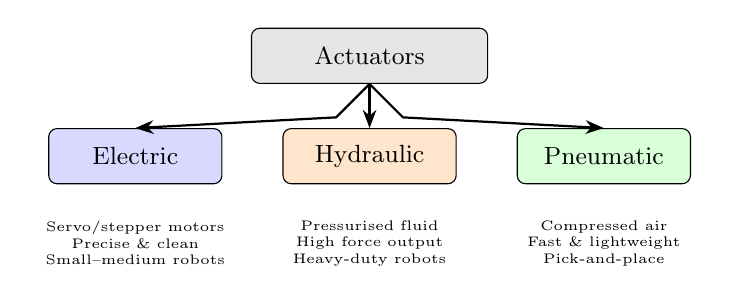
\begin{tikzpicture}[scale=0.85,
  box/.style={draw,rounded corners=3pt,minimum width=2.2cm,
              minimum height=0.7cm,align=center,font=\small},
  arr/.style={-Stealth,thick}]

  \node[box,fill=gray!20,minimum width=3.0cm] (act) at (4,4) {Actuators};

  \node[box,fill=blue!15]    (elec) at (0.5,2.5)   {Electric};
  \node[box,fill=orange!20]  (hyd)  at (4.0,2.5)   {Hydraulic};
  \node[box,fill=green!15]   (pneu) at (7.5,2.5)   {Pneumatic};

  \draw[arr] (act.south) -- ++(-0.5,-0.5) -- (elec.north);
  \draw[arr] (act.south) -- (hyd.north);
  \draw[arr] (act.south) -- ++(0.5,-0.5)  -- (pneu.north);

  \node[font=\tiny,align=center,text width=2.5cm] at (0.5,1.2)
    {Servo/stepper motors\\Precise \& clean\\Small--medium robots};
  \node[font=\tiny,align=center,text width=2.5cm] at (4.0,1.2)
    {Pressurised fluid\\High force output\\Heavy-duty robots};
  \node[font=\tiny,align=center,text width=2.5cm] at (7.5,1.2)
    {Compressed air\\Fast \& lightweight\\Pick-and-place};

\end{tikzpicture}
\end{center}

\begin{itemize}[leftmargin=1.5em,itemsep=3pt]
  \item \textbf{Electric actuators:} Powered by DC or AC servo motors or
        stepper motors. High precision, clean operation, easy speed control.
        The most common type in modern industrial robots.
  \item \textbf{Hydraulic actuators:} Use pressurised hydraulic fluid to
        generate large forces or torques. Suitable for heavy payloads and
        where high power density is needed. Disadvantages: fluid leakage,
        maintenance complexity, fire hazard.
  \item \textbf{Pneumatic actuators:} Use compressed air. Very fast and
        lightweight. Used in simple pick-and-place robots. Less precise than
        electric actuators as air is compressible.
  \item \textbf{Piezoelectric actuators:} Use the piezoelectric effect to
        produce very small, precise displacements at high frequencies. Used
        in micro-robotics and fine-positioning stages.
\end{itemize}

\end{tcolorbox}

%%────────────────────────────────────────────────────────────
%% C1-Q7
%%────────────────────────────────────────────────────────────
\item \label{qlabel:C1-Q5}
(a) What are the specifications used to describe a robot? What are different joint drive systems used in robotics? \mk{10}\\
(b) What is a robot manipulator? How are they classified? With necessary sketch, discuss the SCARA robot arm. \mk{10}\\
(c) What is robot vision? Discuss how a robot vision system works. \mk{10}\\
(d) What do you understand by ``Degeneracy'' and ``Dexterity''? \mk{5}
\yr{2017--18}

\begin{tcolorbox}[enhanced,breakable,ansbox,colback=cA!4,colframe=cA,
  boxrule=0.8pt,arc=5pt,
  title={\textbf{Answer}},fonttitle=\bfseries\color{white},colbacktitle=cA]

\textbf{Part (a): Robot Specifications and Joint Drive Systems}

\textbf{Specifications:}
\begin{itemize}[leftmargin=1.5em,itemsep=2pt]
  \item \textbf{Payload:} Maximum weight the robot can carry while maintaining
        accuracy and following the intended path.
  \item \textbf{Reach:} Maximum distance the end-effector can extend from the
        base within the work envelope.
  \item \textbf{Speed:} Rate of motion (m/s or degrees/s) at a specified load.
  \item \textbf{Accuracy:} Ability to position the end-effector at a specified
        target location with minimum error (absolute concept).
  \item \textbf{Repeatability:} Ability to return to the same position
        consistently across multiple cycles (relative concept).
  \item \textbf{Degrees of Freedom (DOF):} Number of independent axes of motion.
  \item \textbf{Workspace/Work Envelope:} Total reachable volume.
  \item \textbf{Resolution:} Smallest incremental movement the robot can make.
\end{itemize}

\textbf{Joint Drive Systems:}
\begin{itemize}[leftmargin=1.5em,itemsep=2pt]
  \item \textbf{Electric drives:} Servo motors or stepper motors. Precise,
        clean, easy to control. Most common in modern robots.
  \item \textbf{Hydraulic drives:} High-force output using pressurised fluid.
        Used in heavy-duty industrial robots and large payloads.
  \item \textbf{Pneumatic drives:} Use compressed air. Fast and lightweight
        but less precise. Common in pick-and-place robots.
  \item \textbf{Piezoelectric drives:} Very small, precise displacements.
        Used in micro-robots and fine-positioning applications.
\end{itemize}

\hrulefill

\textbf{Part (b): Robot Manipulator and SCARA}

A \textbf{robot manipulator} is the main structural body of the robot,
consisting of a series of rigid \emph{links} connected by \emph{joints} that
provide relative motion. It positions the end-effector in the required location
and orientation within the workspace.

\textit{Classification:} See C1-Q4(b) — Cartesian, Cylindrical, Spherical,
Anthropomorphic, SCARA.

\textbf{SCARA (Selectively Compliant Assembly Robot Arm):}
\begin{itemize}[leftmargin=1.5em,itemsep=2pt]
  \item Notation: \textbf{VRO} or \textbf{RRLT}
  \item Has at least two parallel rotary joints with vertical axes (V, R) and
        an additional prismatic joint for vertical motion.
  \item \emph{Selectively compliant} — rigid in the vertical direction (for
        insertion) but compliant horizontally (absorbs lateral misalignment).
  \item Ideal for \textbf{pick-and-place} and \textbf{assembly} tasks.
\end{itemize}


\begin{center}
  \includegraphics[height=0.3\textheight,width=0.75\textwidth,keepaspectratio]{/scara.png}
\end{center}


\hrulefill

\textbf{Part (c): Robot Vision}

\textbf{Robot vision} (machine vision) is the ability of a robot to interpret
visual information from its environment using cameras and image processing.
It allows the robot to identify, locate, and inspect objects.

\textbf{How a Robot Vision System Works:}
\begin{enumerate}[leftmargin=1.5em,itemsep=2pt,label=\arabic*.]
  \item \textbf{Image acquisition:} A camera (CCD/CMOS) captures a 2D or 3D
        image of the scene under controlled lighting.
  \item \textbf{Digitisation:} The analogue image signal is converted to a
        digital pixel array by an A/D converter (frame grabber).
  \item \textbf{Pre-processing:} Noise reduction, contrast enhancement,
        and filtering (e.g.\ edge detection using Sobel or Canny filters).
  \item \textbf{Segmentation:} The image is segmented to isolate objects
        of interest from the background (thresholding, blob detection).
  \item \textbf{Feature extraction:} Geometric features (area, perimeter,
        centroid, orientation) are computed from the segmented regions.
  \item \textbf{Interpretation / Recognition:} Features are matched against
        a model database to identify the object and determine its pose
        (position and orientation).
  \item \textbf{Robot control:} The computed object position is sent to the
        robot controller to guide the end-effector to the correct location.
\end{enumerate}

\hrulefill

\textbf{Part (d): Degeneracy and Dexterity}

\textbf{Degeneracy:} A condition in a robot manipulator where two or more
joints become aligned in the same direction, causing a loss of a degree of
freedom. At a degenerate configuration (also called a \emph{singular
configuration}), the robot loses the ability to move in one or more
Cartesian directions regardless of how joints are commanded. The Jacobian
matrix becomes rank-deficient at singularities.

\textbf{Dexterity:} The ability of a robot manipulator to reach a given point
in space in \emph{multiple orientations}. A highly dexterous robot can place
its end-effector at the same position with different wrist orientations,
giving it greater flexibility. Dexterity is related to the number of DOF
(redundant robots with $>6$ DOF have higher dexterity) and the shape of the
manipulability ellipsoid at a given configuration.

\end{tcolorbox}

%%────────────────────────────────────────────────────────────
%% C1-Q6
%%────────────────────────────────────────────────────────────
\item \label{qlabel:C1-Q4}
(a) What is a Robot? Mention the names and functions of robot accessories. \mk{10}\\
(b) How are robot manipulators classified? Discuss the anthropomorphic type with a suitable notation and sketch. \mk{10}
\yr{2016--17}

\begin{tcolorbox}[enhanced,breakable,ansbox,colback=cA!4,colframe=cA,
  boxrule=0.8pt,arc=5pt,
  title={\textbf{Answer}},fonttitle=\bfseries\color{white},colbacktitle=cA]

\textbf{Part (a): Definition of a Robot and Its Accessories}

\textbf{Definition (ISO):} A robot is an \emph{automatically controlled,
reprogrammable, multipurpose manipulator} programmable in three or more axes,
which may be either fixed in place or mobile, for use in industrial automation
applications.

More generally, a robot is a machine that can sense its environment, process
information, and execute physical tasks autonomously or semi-autonomously.

\textbf{Robot Accessories (Components) and Their Functions:}

\begin{itemize}[leftmargin=1.5em,itemsep=2pt]
  \item \textbf{Manipulator:} The main structural body (links + joints) that
        positions objects in the work volume — the ``arm.''
  \item \textbf{End Effector:} Tool attached to the wrist — interacts with the
        task (grippers, welding guns, drills, spray guns, etc.).
  \item \textbf{Actuators:} Convert energy into motion — the ``muscles.''
        Types: electric (servomotors), hydraulic, pneumatic.
  \item \textbf{Sensors:} Electro-mechanical devices that allow the robot to
        perceive its environment (position encoders, force sensors, vision
        cameras).
  \item \textbf{Processor:} The ``brain'' — runs kinematic calculations,
        determines joint motions, coordinates actions.
  \item \textbf{Controller:} Receives processor data, drives actuators,
        coordinates motion with sensor feedback.
  \item \textbf{Software:} Operating system, kinematic/motion planning
        software, and application-specific task programs.
\end{itemize}

\hrulefill

\textbf{Part (b): Classification of Robot Manipulators}

Robot manipulators are classified by their \textbf{body-and-arm configuration}
(determined by the joint sequence):

\begin{itemize}[leftmargin=1.5em,itemsep=1pt]
  \item \textbf{Cartesian (PPP):} Three prismatic joints — LLL or LOO
  \item \textbf{Cylindrical:} One rotary + two prismatic — TLO
  \item \textbf{Spherical/Polar:} Two rotary + one prismatic — TRL
  \item \textbf{Anthropomorphic (Jointed-arm / Revolute):} Three rotary
        joints — TRR
  \item \textbf{SCARA:} Two parallel revolute + prismatic — VRO or RRLT
\end{itemize}

\textbf{Anthropomorphic (Jointed-Arm) Robot:}

Also called the \textbf{articulated robot}, it most closely resembles the
human arm. Notation: \textbf{TRR} (body-and-arm). The shoulder twists (T),
the upper arm rotates at the shoulder (R), and the forearm rotates at the
elbow (R).

\begin{center}
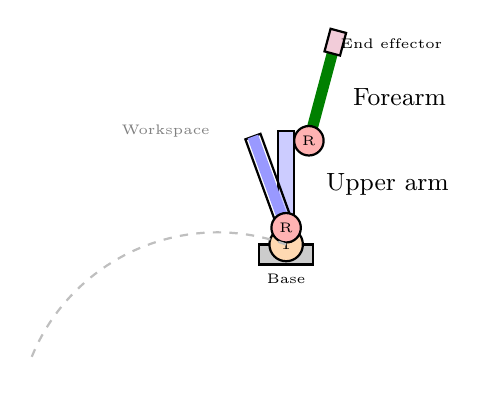
\begin{tikzpicture}[scale=0.85,
  arr/.style={-Stealth,thick,gray}]
  % Base
  \fill[gray!40] (-0.4,0) rectangle (0.4,0.3);
  \draw[thick]   (-0.4,0) rectangle (0.4,0.3);
  \node[font=\tiny,below] at (0,0) {Base};

  % Twist joint (T) at base
  \draw[thick,fill=orange!30] (0,0.3) circle(0.25);
  \node[font=\tiny] at (0,0.3) {T};

  % Link 1 (upper arm) — slanted
  \draw[thick,fill=blue!20] (-0.12,0.55) rectangle (0.12,2.0);
  \draw[thick,rotate around={20:(0,0.55)}]
    (-0.12,0.55) rectangle (0.12,2.0);
  \draw[line width=4pt,blue!40,rotate around={20:(0,0.55)}]
    (0,0.55)--(0,2.0);

  % Shoulder R joint
  \draw[thick,fill=red!30] (0,0.55) circle(0.22);
  \node[font=\tiny] at (0,0.55) {R};

  % Link 2 (forearm) — different angle
  \draw[line width=4pt,green!50!black,rotate around={-15:(0.34,1.85)}]
    (0.34,1.85)--(0.34,3.2);

  % Elbow R joint
  \draw[thick,fill=red!30] (0.34,1.85) circle(0.22);
  \node[font=\tiny] at (0.34,1.85) {R};

  % End effector
  \draw[thick,fill=purple!20,rotate around={-15:(0.34,1.85)}]
    (0.22,3.2) rectangle (0.46,3.55);
  \node[font=\tiny,right=0.1cm] at (0.55,3.3) {End effector};

  % Labels
  \node[font=\small,right=0.3cm] at (0.1,1.2)  {Upper arm};
  \node[font=\small,right=0.3cm] at (0.5,2.5)  {Forearm};

  % Workspace hint
  \draw[dashed,gray!50,thick] (0,0.3)
    arc[start angle=70,end angle=160,radius=3.0];
  \node[font=\tiny,gray] at (-1.8,2.0) {Workspace};
\end{tikzpicture}
\end{center}

\textbf{Advantages:} Largest workspace-to-floor-space ratio; can reach above,
below, and around obstacles. \textbf{Disadvantages:} Complex kinematics;
multiple solutions for inverse kinematics; most complex to program offline.

\end{tcolorbox}

%%────────────────────────────────────────────────────────────
%% C1-Q5
%%────────────────────────────────────────────────────────────
\item \label{qlabel:C1-Q16}
Define payload. Briefly classify robots according to JIRA. \mk{8}
\yr{2015--16}

\begin{tcolorbox}[enhanced,breakable,ansbox,colback=cA!4,colframe=cA,
  boxrule=0.8pt,arc=5pt,
  title={\textbf{Answer}},fonttitle=\bfseries\color{white},colbacktitle=cA]

\variant{C1-Q6(a) — identical question; full answer given there}

\textbf{Payload:} The maximum weight (including end-effector/tooling) the robot
can carry while maintaining its rated accuracy, speed, and path-following
performance.

\textbf{JIRA Classification (6 Classes):}
\begin{enumerate}[leftmargin=*,itemsep=2pt,label=\textbf{Class \arabic*:}]
  \item Manual Manipulator
  \item Fixed Sequence Robot
  \item Variable Sequence Robot
  \item Playback Robot
  \item Numerically Controlled Robot
  \item Intelligent Robot
\end{enumerate}

See \textbf{C1-Q6(a)} for detailed descriptions of each class.

\end{tcolorbox}


\item \label{qlabel:C1-Q7}
Briefly classify robots according to the Robotics Institute of America (RIA). \mk{8}
\yr{2013--14}

\begin{tcolorbox}[enhanced,breakable,ansbox,colback=cA!4,colframe=cA,
  boxrule=0.8pt,arc=5pt,
  title={\textbf{Answer}},fonttitle=\bfseries\color{white},colbacktitle=cA]

The \textbf{Robotics Institute of America (RIA)} classifies robots into
four classes based on their level of programmability and capability:

\begin{enumerate}[leftmargin=*,itemsep=4pt,label=\textbf{Class \arabic*:}]
  \item \textbf{Fixed-Sequence Devices:} Perform a fixed set of operations in
        a predetermined, unalterable sequence. No reprogrammability. Examples:
        simple pick-and-place machines controlled by mechanical stops.
  \item \textbf{Variable-Sequence Devices:} Similar to Class 1 but the
        sequence of operations can be altered relatively easily by the
        operator, typically by changing cams, stops, or wiring. Still limited
        to point-to-point motions.
  \item \textbf{Playback Robots:} Can be programmed by leading the robot
        through the desired task (teach pendant or lead-through) and then
        playing back the memorised motion. Represent the majority of
        industrial robots in use today.
  \item \textbf{Intelligent Robots:} Equipped with sensors (vision, touch,
        force) and AI capabilities. Can adapt their actions in response to
        changes in the environment, make decisions, and perform complex
        unstructured tasks without explicit reprogramming for every variation.
\end{enumerate}

\textit{Note:} The RIA definition of a robot emphasises programmability —
only Classes 3 and 4 are considered true robots under the strict RIA
definition, as they are reprogrammable.

\end{tcolorbox}

%%────────────────────────────────────────────────────────────
%% C1-Q8
%%────────────────────────────────────────────────────────────
\item \label{qlabel:C1-Q8}
Briefly define any two of the following: (i) Payload, (ii) Reach, (iii) Precision. \mk{6}
\yr{2013--14}

\begin{tcolorbox}[enhanced,breakable,ansbox,colback=cA!4,colframe=cA,
  boxrule=0.8pt,arc=5pt,
  title={\textbf{Answer}},fonttitle=\bfseries\color{white},colbacktitle=cA]

\textbf{(i) Payload:}
The \emph{payload} is the maximum weight that the robot can carry (including
the end-effector/tool) while still maintaining all its other specifications
(accuracy, speed, path-following). Operating above the rated payload causes
increased positioning errors, excessive deflection, and potential mechanical
damage.

\textbf{(ii) Reach:}
The \emph{reach} is the maximum distance the robot's end-effector can extend
from the base within its work envelope. It is a function of the link lengths,
joint ranges, and overall configuration. Reach must be considered carefully
before selecting and installing a robot for a given workstation.

\textbf{(iii) Precision (Accuracy):}
\emph{Precision} (or accuracy) is the ability of the robot to position its
end-effector at a specified, commanded location with minimum error. It is an
absolute measure — comparing the actual achieved position to the intended
target position in the world coordinate frame. A robot with high precision
consistently hits the commanded target.

\end{tcolorbox}

%%────────────────────────────────────────────────────────────
%% C1-Q9
%%────────────────────────────────────────────────────────────
\item \label{qlabel:C1-Q9}
What do you understand by the term ``Robot''? Define Payload, Reach, Precision, and Repeatability from the point of view of robot specification. \mk{10}
\yr{2012--13}

\begin{tcolorbox}[enhanced,breakable,ansbox,colback=cA!4,colframe=cA,
  boxrule=0.8pt,arc=5pt,
  title={\textbf{Answer}},fonttitle=\bfseries\color{white},colbacktitle=cA]

\textbf{Definition of a Robot:}

A \textbf{robot} is an automatically controlled, reprogrammable, multipurpose
mechanical device programmable in three or more axes, capable of sensing its
environment and executing physical tasks. The ISO definition emphasises:
automatically controlled, reprogrammable, multipurpose, and three or more
programmable axes. Robots may be fixed or mobile and are used in industrial
automation, healthcare, exploration, and many other fields.

\medskip
\textbf{Robot Specifications:}

\textbf{Payload:} The maximum weight (including tooling/end-effector) the
robot can carry while still meeting its specifications for accuracy, speed,
and path following. Exceeding payload causes accuracy degradation and
mechanical stress.

\textbf{Reach:} The maximum distance from the robot's base to its
end-effector within the work envelope. Determined by link lengths and joint
ranges. A critical parameter for workstation layout design.

\textbf{Precision (Accuracy):} The ability to position the end-effector at
a \emph{commanded target} location with minimum error. An absolute concept
— the discrepancy between the commanded position and the actual position
achieved, measured in the world coordinate frame.

\textbf{Repeatability:} The ability to return to the \emph{same position}
consistently across multiple repetitions of the same task. A relative concept —
measured as the statistical scatter of repeated position measurements about
their mean. A robot may be highly repeatable but inaccurate (if it consistently
goes to the same wrong location) or accurate but not repeatable (if successive
positions scatter around the correct target).

\end{tcolorbox}

%%────────────────────────────────────────────────────────────
%% C1-Q10
%%────────────────────────────────────────────────────────────
\item \label{qlabel:C1-Q11}
(a) Give a brief description of the main components of a robot. \mk{10}\\
(b) What is meant by robot coordinates? With a neat sketch, explain the working space of a cylindrical coordinate robot. \mk{8}
\yr{2011--12}

\begin{tcolorbox}[enhanced,breakable,ansbox,colback=cA!4,colframe=cA,
  boxrule=0.8pt,arc=5pt,
  title={\textbf{Answer}},fonttitle=\bfseries\color{white},colbacktitle=cA]

\textbf{Part (a): Main Components of a Robot}

\variant{C1-Q4(a) — same components listed and described there}

\begin{itemize}[leftmargin=1.5em,itemsep=2pt]
  \item \textbf{Manipulator:} Links and joints — the structural arm that
        positions the end-effector.
  \item \textbf{End Effector:} Tool at the wrist (gripper, drill, welding gun)
        that interacts with the task.
  \item \textbf{Actuators:} Convert energy to motion — electric servos,
        hydraulic cylinders, or pneumatic pistons.
  \item \textbf{Processor:} The computer brain that runs kinematic
        calculations and coordinates all actions.
  \item \textbf{Controller:} Drives actuators based on processor commands
        and sensor feedback.
  \item \textbf{Sensors:} Provide feedback on position, force, and
        environment (encoders, cameras, force/torque sensors).
  \item \textbf{Software:} OS, kinematic motion software, and application
        task programs.
\end{itemize}

\hrulefill

\textbf{Part (b): Robot Coordinates and Cylindrical Robot Workspace}

\textbf{Robot coordinates} refer to the coordinate system used to describe
the position and orientation of the robot's end-effector and joints. The
main coordinate frames are:
\begin{itemize}[leftmargin=1.5em,itemsep=1pt]
  \item \textbf{World/Universe frame ($F_{xyz}$):} Fixed global reference.
  \item \textbf{Joint coordinates:} Values of each joint variable
        ($d_i$, $\theta_i$).
  \item \textbf{Tool/End-effector frame:} Attached to the end-effector.
\end{itemize}

\textbf{Cylindrical coordinate robot} (notation: \textbf{TLO}) uses one
rotary joint (T — rotation about vertical axis) and two prismatic joints
(L — vertical translation, O — horizontal extension). The workspace is a
\emph{hollow cylinder} (annular cylinder) shape.

\begin{center}
  \includegraphics[height=0.3\textheight,width=0.75\textwidth,keepaspectratio]{/crobot.png}
\end{center}

The cylindrical robot can rotate 360° about the vertical axis, extend the arm
radially, and move up/down — creating a hollow-cylinder workspace. It cannot
reach directly below itself or very close to its own axis.

\end{tcolorbox}

%%────────────────────────────────────────────────────────────
%% C1-Q12
%%────────────────────────────────────────────────────────────
\item \label{qlabel:C1-Q10}
(a) Describe the different parameters used to depict the specification of a robot. \mk{15}\\
(b) Mention some notable applications of robots. \mk{8}
\yr{2010--11}

\begin{tcolorbox}[enhanced,breakable,ansbox,colback=cA!4,colframe=cA,
  boxrule=0.8pt,arc=5pt,
  title={\textbf{Answer}},fonttitle=\bfseries\color{white},colbacktitle=cA]

\textbf{Part (a): Robot Specification Parameters}

\begin{itemize}[leftmargin=1.5em,itemsep=3pt]
  \item \textbf{Payload:} Maximum weight the robot can handle (including
        end-effector) within rated performance. Typical industrial robots:
        5--500\,kg.
  \item \textbf{Reach (Work Envelope):} The total volume or area reachable
        by the end-effector. Determined by link lengths and joint travel
        limits.
  \item \textbf{Speed:} Maximum velocity of the end-effector or joint axes
        (m/s or deg/s), specified at a given load. Higher speed reduces
        cycle time.
  \item \textbf{Accuracy:} Ability to position the end-effector at the
        commanded location. Expressed as maximum position error (e.g.\
        $\pm$0.1\,mm). An absolute specification.
  \item \textbf{Repeatability:} Statistical consistency of returning to
        the same location (e.g.\ $\pm$0.05\,mm). A relative specification,
        typically better than accuracy for industrial robots.
  \item \textbf{Resolution:} Smallest increment of motion the control
        system can command. Limited by encoder resolution and mechanical
        backlash.
  \item \textbf{Degrees of Freedom (DOF):} Number of independent axes.
        Most industrial robots: 6 DOF (3 for positioning + 3 for orientation).
  \item \textbf{Drive System:} Electric, hydraulic, or pneumatic — affects
        force output, precision, and cleanliness.
  \item \textbf{Control Method:} Point-to-point (PTP) or continuous-path
        (CP) control capability.
  \item \textbf{Compliance:} Ability of the robot to yield elastically
        under force without damage; important for assembly tasks.
\end{itemize}

\hrulefill

\textbf{Part (b): Notable Applications of Robots}

\begin{itemize}[leftmargin=1.5em,itemsep=2pt]
  \item \textbf{Manufacturing:} Welding (spot and arc), painting/coating,
        assembly, machine tending, material handling.
  \item \textbf{Healthcare:} Surgical robots (da Vinci), rehabilitation
        exoskeletons, drug dispensing.
  \item \textbf{Agriculture:} Automated harvesting, planting, pesticide
        spraying.
  \item \textbf{Exploration:} Mars rovers (Curiosity, Perseverance),
        deep-sea underwater robots, nuclear facility inspection.
  \item \textbf{Military/Defence:} Bomb disposal (EOD robots), surveillance
        drones, autonomous vehicles.
  \item \textbf{Logistics:} Warehouse automation (Amazon Kiva robots),
        sorting systems, last-mile delivery drones.
  \item \textbf{Construction:} Bricklaying robots, concrete 3D printing,
        inspection drones.
  \item \textbf{Service:} Household cleaning (Roomba), social robots
        (Pepper), hotel service robots.
  \item \textbf{Education:} Teaching STEM (LEGO Mindstorms, NAO robots).
\end{itemize}

\end{tcolorbox}

%%────────────────────────────────────────────────────────────
%% C1-Q11
%%────────────────────────────────────────────────────────────
\item \label{qlabel:C1-Q12}
(a) What are the steps in Machine Vision Application? \mk{5}\\
(b) Describe the types of gripper used in Industrial Robot Applications. \mk{10}
\yr{2008--09}

\begin{tcolorbox}[enhanced,breakable,ansbox,colback=cA!4,colframe=cA,
  boxrule=0.8pt,arc=5pt,
  title={\textbf{Answer}},fonttitle=\bfseries\color{white},colbacktitle=cA]

\textbf{Part (a): Steps in Machine Vision Application}

\variant{C1-Q5(c) — full details given there}

The key steps are:
\begin{enumerate}[leftmargin=1.5em,itemsep=1pt,label=\arabic*.]
  \item Image acquisition (camera capture)
  \item Digitisation (A/D conversion to pixel array)
  \item Pre-processing (filtering, noise removal, contrast enhancement)
  \item Segmentation (isolating objects from background)
  \item Feature extraction (area, centroid, orientation)
  \item Interpretation/object recognition (matching against model)
  \item Robot control (sending position data to controller)
\end{enumerate}

\hrulefill

\textbf{Part (b): Types of Grippers}

\begin{itemize}[leftmargin=1.5em,itemsep=3pt]
  \item \textbf{Mechanical grippers:} Two or more fingers actuated by
        pneumatic, electric, or hydraulic drives through a linkage. The
        most common type — used for rigid parts of varying shapes. Can
        be parallel-jaw (translate) or angular (rotate).
  \item \textbf{Vacuum (suction cup) grippers:} Use vacuum suction cups
        (made of rubber) to grip flat, smooth, and fragile objects such as
        glass panels, circuit boards, and sheet metal. Require a vacuum
        pump or venturi generator.
  \item \textbf{Magnetic grippers:} Use electromagnets or permanent
        magnets to grip ferrous (iron or steel) workpieces. Simple, fast,
        and can handle irregular shapes. Electromagnets allow easy
        on/off switching.
  \item \textbf{Adhesive grippers:} Use adhesive pads or sticky surfaces
        to grip lightweight, flexible, or deformable objects such as fabric,
        foam, or thin film.
  \item \textbf{Simple mechanical devices:} Hooks, scoops, ladles, and
        nails used for specialised tasks such as lifting coils, scooping
        bulk materials, or handling irregularly shaped objects.
  \item \textbf{Tool-based end-effectors:} Drilling spindles, grinding
        wheels, welding torches, spray guns — technically end-effectors
        rather than grippers, but classified under end-of-arm tooling.
\end{itemize}

\end{tcolorbox}

%%────────────────────────────────────────────────────────────
%% C1-Q13
%%────────────────────────────────────────────────────────────
\item \label{qlabel:C1-Q13}
What do you mean by cylindrical coordinate robot? Draw top and side views of workspace for this type. \mk{5}
\yr{2006--07}

\begin{tcolorbox}[enhanced,breakable,ansbox,colback=cA!4,colframe=cA,
  boxrule=0.8pt,arc=5pt,
  title={\textbf{Answer}},fonttitle=\bfseries\color{white},colbacktitle=cA]

A \textbf{cylindrical coordinate robot} uses a combination of one rotary
joint (T — rotation about the vertical axis) and two prismatic joints
(L — vertical translation, O — radial horizontal extension). Its joint
notation is \textbf{TLO}.

The robot positions its end-effector using cylindrical coordinates
$(r,\, \alpha,\, z)$ — radial distance $r$, rotation angle $\alpha$, and
height $z$.

\textbf{Workspace (Top and Side Views):}

\variant{C1-Q11(b) — identical workspace diagrams given there}

The workspace is a \textbf{hollow cylinder (annular cylinder):}
\begin{itemize}[leftmargin=1.5em,itemsep=1pt]
  \item \textbf{Top view:} Annular ring — can reach all angles (360°) between
        a minimum and maximum radial distance.
  \item \textbf{Side view:} Rectangle — shows the range of vertical height
        and radial extension.
\end{itemize}

\textbf{Advantages:} Can reach all around itself; radial and height axes
are rigid. \textbf{Disadvantages:} Cannot reach above itself; linear axes
are harder to seal against contamination.

\end{tcolorbox}

%%────────────────────────────────────────────────────────────
%% C1-Q14
%%────────────────────────────────────────────────────────────
\item \label{qlabel:C1-Q14}
``One machine can do the work of a hundred ordinary men, but no machine can do the work of one extraordinary man.'' --- Discuss. \mk{5}
\yr{2004--05, 2005--06}

\begin{tcolorbox}[enhanced,breakable,ansbox,colback=cA!4,colframe=cA,
  boxrule=0.8pt,arc=5pt,
  title={\textbf{Answer}},fonttitle=\bfseries\color{white},colbacktitle=cA]

This quote by Elbert Hubbard captures the fundamental distinction between
machine capability and human ingenuity.

\textbf{``One machine can do the work of a hundred ordinary men'':}

This reflects the well-known advantages of robots and automation:
\begin{itemize}[leftmargin=1.5em,itemsep=1pt]
  \item Robots work continuously 24/7 without fatigue, breaks, or boredom.
  \item They perform repetitive tasks with consistent precision and speed that
        far exceeds an average human worker.
  \item They can operate in hazardous environments (radiation, extreme heat/cold,
        toxic atmospheres) with no risk.
  \item A single robotic cell can replace multiple human workers in
        high-volume manufacturing (e.g.\ welding, painting, assembly).
\end{itemize}

\textbf{``But no machine can do the work of one extraordinary man'':}

This reflects the critical \emph{limitations} of robots compared to
exceptional human capability:
\begin{itemize}[leftmargin=1.5em,itemsep=1pt]
  \item Robots \textbf{lack creativity, intuition, and innovation} — they
        cannot invent new solutions or think outside their programming.
  \item They have \textbf{limited cognition and decision-making} in
        unstructured or unpredictable situations.
  \item They cannot \textbf{understand context, emotion, or ethics} the way
        an exceptional human can.
  \item An extraordinary human can \textbf{adapt instantly} to novel problems,
        exercise judgement, and find solutions that were never anticipated.
  \item Exceptional human contributions (scientific breakthroughs, artistic
        masterpieces, moral leadership) remain beyond any current or foreseeable
        machine.
\end{itemize}

\textbf{Conclusion:} Robots are powerful tools for amplifying human productivity
in well-defined, repetitive tasks. However, they complement rather than replace
human intelligence, creativity, and wisdom — especially at the highest levels
of human achievement. The role of robotics is to free extraordinary humans from
ordinary work, allowing them to focus on what machines can never do.

\end{tcolorbox}

%%────────────────────────────────────────────────────────────
%% C1-Q15
%%────────────────────────────────────────────────────────────
\item \label{qlabel:C1-Q15}
(a) Draw the basic configurations for: (i) PPP, (ii) RRP, (iii) RYP. \mk{9}\\
(b) How do you compare end effectors and manipulator? \mk{7}\\
(c) Based on the task to be accomplished, how do you recommend the use of hydraulic vs electric drive systems? \mk{8}
\yr{2003--04}

\begin{tcolorbox}[enhanced,breakable,ansbox,colback=cA!4,colframe=cA,
  boxrule=0.8pt,arc=5pt,
  title={\textbf{Answer}},fonttitle=\bfseries\color{white},colbacktitle=cA]

\textbf{Part (a): Basic Configurations}

\textbf{Note on notation:} PPP $\equiv$ LLL (three prismatic), RRP $\equiv$
two rotational + one prismatic. RYP uses Roll/Yaw/Pitch to describe wrist
motion types (all rotary) — equivalent to RRT or similar wrist notation.

\textbf{(i) PPP (Cartesian / Gantry robot — LLL):}
Three mutually perpendicular linear joints. Motion along X, Y, Z axes.

\begin{center}
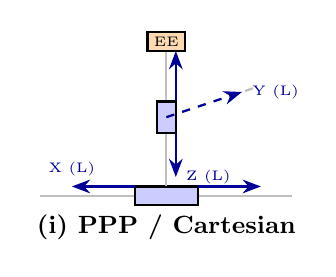
\begin{tikzpicture}[scale=0.80,
  arr/.style={-Stealth,thick,blue!60!black}]
  % X rail
  \draw[thick,gray!50] (0,0)--(4,0);
  \fill[blue!20] (1.5,-0.15) rectangle (2.5,0.15);
  \draw[thick]   (1.5,-0.15) rectangle (2.5,0.15);
  \draw[arr] (1.5,0.15) -- (0.5,0.15) node[above,font=\tiny]{X (L)};
  \draw[arr] (2.5,0.15) -- (3.5,0.15);

  % Y rail (vertical)
  \draw[thick,gray!50] (2.0,0.15)--(2.0,2.5);
  \fill[blue!20] (1.85,1.0) rectangle (2.15,1.5);
  \draw[thick]   (1.85,1.0) rectangle (2.15,1.5);
  \draw[arr] (2.15,1.0) -- (2.15,0.3) node[right,font=\tiny]{Z (L)};
  \draw[arr] (2.15,1.5) -- (2.15,2.3);

  % Z rail (depth)
  \draw[thick,gray!50,dashed] (2.0,1.25)--(3.5,1.75);
  \draw[arr,dashed] (2.0,1.25) -- (3.2,1.65) node[right,font=\tiny]{Y (L)};

  % End effector
  \fill[orange!30] (1.7,2.3) rectangle (2.3,2.6);
  \draw[thick] (1.7,2.3) rectangle (2.3,2.6);
  \node[font=\tiny] at (2.0,2.45) {EE};
  \node[font=\small\bfseries] at (2.0,-0.5) {(i) PPP / Cartesian};
\end{tikzpicture}
\end{center}

\textbf{(ii) RRP (Two rotary + one prismatic — e.g.\ Spherical/Polar robot TRL):}

\begin{center}
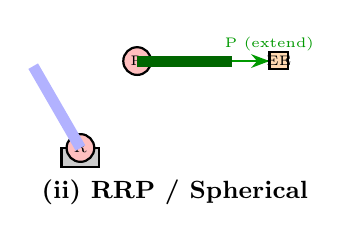
\begin{tikzpicture}[scale=0.80,arr/.style={-Stealth,thick}]
  % Base
  \fill[gray!40] (-0.3,0) rectangle (0.3,0.3);
  \draw[thick]   (-0.3,0) rectangle (0.3,0.3);
  % R1 joint (rotation 1 — horizontal)
  \draw[thick,fill=red!25] (0,0.3) circle(0.22);
  \node[font=\tiny] at (0,0.3) {R};
  % Link going up-right
  \draw[line width=4pt,blue!30,rotate around={30:(0,0.3)}]
    (0,0.3)--(0,1.8);
  % R2 joint
  \fill[red!25] (0.9,1.68) circle(0.22);
  \draw[thick]  (0.9,1.68) circle(0.22);
  \node[font=\tiny] at (0.9,1.68) {R};
  % Prismatic extending arm
  \draw[line width=4pt,green!40!black] (0.9,1.68)--(2.4,1.68);
  \draw[thick,dashed] (2.4,1.68)--(3.1,1.68);
  \draw[-Stealth,thick,green!60!black] (2.4,1.68)--(3.0,1.68)
    node[above,font=\tiny]{P (extend)};
  % End effector
  \fill[orange!30] (3.0,1.55) rectangle (3.3,1.82);
  \draw[thick]     (3.0,1.55) rectangle (3.3,1.82);
  \node[font=\tiny] at (3.15,1.68) {EE};
  \node[font=\small\bfseries] at (1.5,-0.4) {(ii) RRP / Spherical};
\end{tikzpicture}
\end{center}

\textbf{(iii) RYP (Roll-Yaw-Pitch — wrist configuration, all rotary):}
This describes a 3-DOF wrist assembly with Roll (R), Yaw (T), and Pitch (R)
joints — notation \textbf{RTR} or \textbf{RRT} in standard form.

\begin{center}
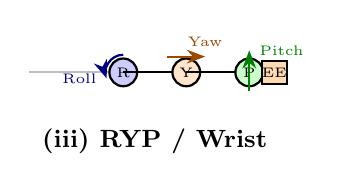
\begin{tikzpicture}[scale=0.80,arr/.style={-Stealth,thick}]
  % Arm end
  \draw[thick,gray!50] (0,1.0)--(1.5,1.0);
  % Roll joint
  \draw[thick,fill=blue!20] (1.5,1.0) circle(0.22);
  \node[font=\tiny] at (1.5,1.0) {R};
  \draw[arr,blue!50!black] (1.5,1.28)
    arc[start angle=90,end angle=200,radius=0.28]
    node[left,font=\tiny]{Roll};
  % Yaw joint
  \draw[thick] (1.5,1.0)--(2.5,1.0);
  \draw[thick,fill=orange!20] (2.5,1.0) circle(0.22);
  \node[font=\tiny] at (2.5,1.0) {Y};
  \draw[arr,orange!60!black] (2.2,1.25)--(2.8,1.25)
    node[above,font=\tiny]{Yaw};
  % Pitch joint
  \draw[thick] (2.5,1.0)--(3.5,1.0);
  \draw[thick,fill=green!20] (3.5,1.0) circle(0.22);
  \node[font=\tiny] at (3.5,1.0) {P};
  \draw[arr,green!50!black] (3.5,0.7)--(3.5,1.35)
    node[right,font=\tiny]{Pitch};
  % End effector
  \fill[orange!30] (3.7,0.82) rectangle (4.1,1.18);
  \draw[thick]     (3.7,0.82) rectangle (4.1,1.18);
  \node[font=\tiny] at (3.9,1.0) {EE};
  \node[font=\small\bfseries] at (2.0,-0.1) {(iii) RYP / Wrist};
\end{tikzpicture}
\end{center}

\hrulefill

\textbf{Part (b): End Effectors vs.\ Manipulator}

\begin{center}
\small
\begin{tabularx}{\linewidth}{@{}lXX@{}}
\toprule
\textbf{Aspect}    & \textbf{Manipulator}                  & \textbf{End Effector} \\
\midrule
Definition         & Main structural body (links \& joints) & Tool attached to wrist \\
Function           & Position and orient the wrist in space & Interact with the task/workpiece \\
DOF contribution   & Provides all positioning DOF           & May add orientation DOF \\
Standardisation    & Generally standardised per robot model & Task-specific; custom-designed \\
Interchangeability & Fixed part of the robot system         & Swappable for different tasks \\
Power source       & Integrated into robot                  & Separate power (electric/pneumatic) \\
Examples           & Links, joints, arm assembly            & Grippers, drills, welding guns \\
\bottomrule
\end{tabularx}
\end{center}

\hrulefill

\textbf{Part (c): Hydraulic vs.\ Electric Drive Systems — Task-Based Selection}

\begin{center}
\small
\begin{tabular}{@{}lll@{}}
\toprule
\textbf{Criterion}        & \textbf{Hydraulic}                & \textbf{Electric} \\
\midrule
Force/Torque output       & Very high (heavy payloads)        & Low-to-medium \\
Precision/Accuracy        & Lower (compressibility of fluid)  & Higher (encoders) \\
Speed                     & High                              & Medium-high \\
Cleanliness               & Risk of oil leakage               & Clean, no fluids \\
Maintenance               & Complex (seals, pumps, filters)   & Simple \\
Task suitability          & Heavy lifting, press, forging     & Assembly, electronics, lab \\
\bottomrule
\end{tabular}
\end{center}

\textbf{Recommendation:}
\begin{itemize}[leftmargin=1.5em,itemsep=1pt]
  \item Use \textbf{hydraulic} drives for: heavy payload handling
        ($>$100\,kg), forging/pressing, underwater robots, construction
        equipment, and large industrial manipulators.
  \item Use \textbf{electric} drives for: precision assembly, electronics
        manufacturing, medical robots, clean-room environments, and
        any application requiring high accuracy and repeatability.
\end{itemize}

\end{tcolorbox}

%%────────────────────────────────────────────────────────────
%% C1-Q16
%%────────────────────────────────────────────────────────────

%% ============================================================
%%  Section C1 — Introduction to Robotics
%%  Question Bank — Answer Snippets
%%  Paste inside the C1 \begin{enumerate} ... \end{enumerate}
%% ============================================================

%%────────────────────────────────────────────────────────────
%% C1-Q1
%%────────────────────────────────────────────────────────────
\end{enumerate}

%%══════════════════════════════════════════════════════════════════════
%% SECTION C2 — Transformations & Rotation Matrices
%%══════════════════════════════════════════════════════════════════════
\secdivider{Section C2}{Plane, Rotational \& Spatial Motion; Transformations}{cB}{cB}
\markboth{C2 --- Transformations \& Rotation Matrices}{}
\label{sec:C2}
\titleformat{\section}{\large\bfseries\color{cB}}{}{0em}{}[\titlerule]
\section{C2 --- Transformations \& Rotation Matrices}

%% ══════════════════════════════════════════════════════════════════════
%% C2 — Transformations & Rotation Matrices  |  ANSWERS
%% ══════════════════════════════════════════════════════════════════════

\begin{enumerate}
\item \label{qlabel:C2-Q1}
(a) Derive a formula by which the description of a point can be changed
from one frame to another, where the frames have the same origin but
different axis orientations. \mk{10}\\
(b) Frame $\{B\}$ is rotated relative to $\{A\}$ about z-axis by
45\textdegree, then translated 2 units in $\hat{X}_A$ and 3 units in
$\hat{Y}_A$. Find ${}^AP$ if ${}^BP = [3\;7\;0]^T$. \mk{10}\\
(c) A point $P = [3\;0\;3]^T$ is subjected to: rotation about y-axis,
then translation along x-axis, then rotation about z-axis. Final
coordinates are $[4\;4\;2]^T$. Find possible transformation
variables. \mk{15}
\yr{2023--24}

\begin{tcolorbox}[enhanced,breakable,ansbox,colback=cB!4,colframe=cB,
  boxrule=0.8pt,arc=5pt,
  title={\textbf{Answer}},fonttitle=\bfseries\color{white},
  colbacktitle=cB]

%% ── Part (a) ──────────────────────────────────────────────────────
\textbf{Part (a): Changing Frame Description (Same Origin, Different
Orientation)}

\medskip
Let frame $\{A\}$ and frame $\{B\}$ share the same origin $O$ but have
different axis orientations. Express the unit vectors of $\{B\}$ in
$\{A\}$ coordinates as $\hat{u}$, $\hat{v}$, $\hat{w}$. Any point $P$
has the same physical location in both frames. In $\{B\}$:
\[
  {}^BP = p_u\,\hat{u} + p_v\,\hat{v} + p_w\,\hat{w}
\]

Expanding each unit vector in $\{A\}$ coordinates:
\[
  {}^AP
  = p_u\begin{bmatrix}u_x\\u_y\\u_z\end{bmatrix}
  + p_v\begin{bmatrix}v_x\\v_y\\v_z\end{bmatrix}
  + p_w\begin{bmatrix}w_x\\w_y\\w_z\end{bmatrix}
  = \begin{bmatrix}
      u_x & v_x & w_x\\
      u_y & v_y & w_y\\
      u_z & v_z & w_z
    \end{bmatrix}
    \begin{bmatrix}p_u\\p_v\\p_w\end{bmatrix}
\]

This defines the rotation matrix ${}^A_BR$ (read: ``rotation of $\{B\}$
relative to $\{A\}$''):
\[
  \boxed{{}^AP = {}^A_BR\;{}^BP}, \qquad
  {}^A_BR =
  \begin{bmatrix}
    u_x & v_x & w_x\\
    u_y & v_y & w_y\\
    u_z & v_z & w_z
  \end{bmatrix}
\]

Each \emph{column} of ${}^A_BR$ is a unit vector of $\{B\}$ expressed in
$\{A\}$. Each element $R_{ij} = \hat{e}^A_i \cdot \hat{e}^B_j$ is the
direction cosine between the $i$-th axis of $\{A\}$ and the $j$-th axis
of $\{B\}$.

\medskip
%% ── Part (b) ──────────────────────────────────────────────────────
\textbf{Part (b): Numerical Computation of ${}^AP$}

\medskip
\textbf{Step 1 — Rotation matrix ${}^A_BR_z(45\textdegree)$:}
\[
  {}^A_BR_z(45\textdegree)
  = \begin{bmatrix}
      \cos45\textdegree & -\sin45\textdegree & 0 \\
      \sin45\textdegree &  \cos45\textdegree & 0 \\
      0 & 0 & 1
    \end{bmatrix}
  = \begin{bmatrix}
      \dfrac{1}{\sqrt{2}} & -\dfrac{1}{\sqrt{2}} & 0 \\[8pt]
      \dfrac{1}{\sqrt{2}} &  \dfrac{1}{\sqrt{2}} & 0 \\[8pt]
      0 & 0 & 1
    \end{bmatrix}
\]

\textbf{Step 2 — Homogeneous transformation matrix ${}^AT_B$:}

Since $\{B\}$ is first rotated then translated by
${}^AP_{B\text{org}} = [2\;3\;0]^T$:
\[
  {}^AT_B
  = \begin{bmatrix}
      \dfrac{1}{\sqrt{2}} & -\dfrac{1}{\sqrt{2}} & 0 & 2 \\[8pt]
      \dfrac{1}{\sqrt{2}} &  \dfrac{1}{\sqrt{2}} & 0 & 3 \\[8pt]
      0 & 0 & 1 & 0 \\
      0 & 0 & 0 & 1
    \end{bmatrix}
\]

\textbf{Step 3 — Compute ${}^AP = {}^AT_B\;{}^BP$:}
\[
  {}^AP
  = {}^A_BR_z(45\textdegree)\;{}^BP + {}^AP_{B\text{org}}
  = \begin{bmatrix}
      3\cos45\textdegree - 7\sin45\textdegree + 2 \\[4pt]
      3\sin45\textdegree + 7\cos45\textdegree + 3 \\[4pt]
      0
    \end{bmatrix}
  = \begin{bmatrix}
      \dfrac{3}{\sqrt{2}} - \dfrac{7}{\sqrt{2}} + 2 \\[8pt]
      \dfrac{3}{\sqrt{2}} + \dfrac{7}{\sqrt{2}} + 3 \\[8pt]
      0
    \end{bmatrix}
\]

\[
  \boxed{{}^AP = \begin{bmatrix}2 - 2\sqrt{2}\\[4pt] 3 + 5\sqrt{2}\\[4pt] 0\end{bmatrix}
  \approx \begin{bmatrix}-0.828\\10.071\\0\end{bmatrix}}
\]

\medskip
%% ── Part (c) ──────────────────────────────────────────────────────
\textbf{Part (c): Finding Transformation Variables}

\medskip
Transformation sequence applied to $P_0 = [3\;0\;3]^T$:
\[
  \mathrm{Rot}(y,\theta) \;\longrightarrow\;
  \mathrm{Trans}(x,d) \;\longrightarrow\;
  \mathrm{Rot}(z,\phi) \;\longrightarrow\;
  P_f = [4\;4\;2]^T
\]

\textbf{Step 1 — After $\mathrm{Rot}(y,\theta)$:}
\[
  R_y(\theta) = \begin{bmatrix}
    \cos\theta & 0 & \sin\theta\\
    0 & 1 & 0\\
    -\sin\theta & 0 & \cos\theta
  \end{bmatrix}
  \implies
  P_1 = \begin{bmatrix}
    3\cos\theta + 3\sin\theta \\
    0 \\
    -3\sin\theta + 3\cos\theta
  \end{bmatrix}
\]

\textbf{Step 2 — After $\mathrm{Trans}(x,d)$:}
\[
  P_2 = \begin{bmatrix}
    3\cos\theta + 3\sin\theta + d \\ 0 \\ -3\sin\theta + 3\cos\theta
  \end{bmatrix}
\]

\textbf{Step 3 — After $\mathrm{Rot}(z,\phi)$:}
\[
  P_3 = \begin{bmatrix}
    (3\cos\theta + 3\sin\theta + d)\cos\phi \\
    (3\cos\theta + 3\sin\theta + d)\sin\phi \\
    3\cos\theta - 3\sin\theta
  \end{bmatrix}
  \stackrel{!}{=} \begin{bmatrix}4\\4\\2\end{bmatrix}
\]

\textbf{Solving the three equations:}

\begin{enumerate}[label=\textbf{\roman*.}]
  \item \textbf{From $z$-component} (unchanged by $\mathrm{Trans}(x)$
    and $\mathrm{Rot}(z)$):
    \[
      3\cos\theta - 3\sin\theta = 2
      \implies \sqrt{2}\cos(\theta+45\textdegree) = \dfrac{2}{3} \cdot \dfrac{\sqrt{2}}{\sqrt{2}}
    \]
    Writing $3(\cos\theta - \sin\theta) = 2$ as $R\cos(\theta+\psi)=2$
    with $R = 3\sqrt{2}$, $\psi=45\textdegree$:
    \[
      \cos(\theta + 45\textdegree) = \frac{2}{3\sqrt{2}}
      \implies \theta + 45\textdegree = \pm\cos^{-1}\!\left(\frac{\sqrt{2}}{3}\right)
      \implies \boxed{\theta \approx 16.87\textdegree}
    \]

  \item \textbf{From $x$- and $y$-components:}
    Since $P_{2y} = 0$, after $\mathrm{Rot}(z,\phi)$:
    \[
      x_3 = x_2\cos\phi = 4, \qquad y_3 = x_2\sin\phi = 4
      \implies \tan\phi = 1 \implies \boxed{\phi = 45\textdegree}
    \]
    Then $x_2 = \dfrac{4}{\cos45\textdegree} = 4\sqrt{2}$, so:
    \[
      d = 4\sqrt{2} - (3\cos\theta + 3\sin\theta)
      \approx 5.657 - 3.742
      \implies \boxed{d \approx 1.915\text{ units}}
    \]
\end{enumerate}

\textbf{Summary:}
\[
  \theta \approx 16.87\textdegree,\qquad d \approx 1.915\text{ units},\qquad \phi = 45\textdegree
\]

\textit{Note: A second mathematical solution $\theta \approx -106.87\textdegree$,
$d \approx 9.40$ also satisfies the equations but is typically rejected
due to physical joint constraints.}

\end{tcolorbox}

%% ─────────────────────────────────────────────────────────────────────
%% C2-Q2
%% ─────────────────────────────────────────────────────────────────────
\item \label{qlabel:C2-Q2}
Frame B is rotated 90\textdegree\ about z-axis, then translated 3 and 5
units relative to n- and o-axes, then rotated 90\textdegree\ about
n-axis, then 90\textdegree\ about y-axis.\\
(i) Write the equation describing the motion.
(ii) Find new location and orientation.
\[
  B = \begin{pmatrix}
    0&1&0&1\\1&0&0&1\\0&0&{-1}&1\\0&0&0&1
  \end{pmatrix}
\]
\mk{15}
\yr{2023--24}

\begin{tcolorbox}[enhanced,breakable,ansbox,colback=cB!4,colframe=cB,
  boxrule=0.8pt,arc=5pt,
  title={\textbf{Solution}},fonttitle=\bfseries\color{white},
  colbacktitle=cB]

\textbf{(i) Equation of Motion}

The transformations applied in sequence:
\[
  B_{\text{new}} = R_y(90\textdegree)\cdot R_z(90\textdegree)\cdot B
                   \cdot \mathrm{Trans}(3,5,0)\cdot R_n(90\textdegree)
\]

\medskip
\textbf{(ii) Individual Transformation Matrices}

\[
  R_z(90\textdegree) =
  \begin{pmatrix}0&-1&0&0\\1&0&0&0\\0&0&1&0\\0&0&0&1\end{pmatrix}
  \qquad
  \mathrm{Trans}(3,5,0) =
  \begin{pmatrix}1&0&0&3\\0&1&0&5\\0&0&1&0\\0&0&0&1\end{pmatrix}
\]

\[
  R_n(90\textdegree) =
  \begin{pmatrix}1&0&0&0\\0&0&-1&0\\0&1&0&0\\0&0&0&1\end{pmatrix}
  \qquad
  R_y(90\textdegree) =
  \begin{pmatrix}0&0&1&0\\0&1&0&0\\-1&0&0&0\\0&0&0&1\end{pmatrix}
\]

\medskip
\textbf{Step 1 —} $R_z(90\textdegree)\cdot B$:
\[
  \begin{pmatrix}0&-1&0&0\\1&0&0&0\\0&0&1&0\\0&0&0&1\end{pmatrix}
  \begin{pmatrix}0&1&0&1\\1&0&0&1\\0&0&{-1}&1\\0&0&0&1\end{pmatrix}
  =
  \begin{pmatrix}-1&0&0&-1\\0&1&0&1\\0&0&{-1}&1\\0&0&0&1\end{pmatrix}
\]

\medskip
\textbf{Step 2 —} $(\cdots)\cdot\mathrm{Trans}(3,5,0)$:
\[
  \begin{pmatrix}-1&0&0&-1\\0&1&0&1\\0&0&{-1}&1\\0&0&0&1\end{pmatrix}
  \begin{pmatrix}1&0&0&3\\0&1&0&5\\0&0&1&0\\0&0&0&1\end{pmatrix}
  =
  \begin{pmatrix}-1&0&0&-4\\0&1&0&6\\0&0&{-1}&1\\0&0&0&1\end{pmatrix}
\]

\medskip
\textbf{Step 3 —} $(\cdots)\cdot R_n(90\textdegree)$:
\[
  \begin{pmatrix}-1&0&0&-4\\0&1&0&6\\0&0&{-1}&1\\0&0&0&1\end{pmatrix}
  \begin{pmatrix}1&0&0&0\\0&0&-1&0\\0&1&0&0\\0&0&0&1\end{pmatrix}
  =
  \begin{pmatrix}-1&0&0&-4\\0&0&-1&6\\0&-1&0&1\\0&0&0&1\end{pmatrix}
\]

\medskip
\textbf{Step 4 —} $R_y(90\textdegree)\cdot(\cdots)$:
\[
  \begin{pmatrix}0&0&1&0\\0&1&0&0\\-1&0&0&0\\0&0&0&1\end{pmatrix}
  \begin{pmatrix}-1&0&0&-4\\0&0&-1&6\\0&-1&0&1\\0&0&0&1\end{pmatrix}
  =
  \begin{pmatrix}0&-1&0&1\\0&0&-1&6\\1&0&0&4\\0&0&0&1\end{pmatrix}
\]

\medskip
\textbf{Result:}
\[
  \boxed{B_{\text{new}} =
  \begin{pmatrix}0&-1&0&1\\0&0&-1&6\\1&0&0&4\\0&0&0&1\end{pmatrix}}
\]

The new position of the origin is $(1,\ 6,\ 4)$ and the orientation
is given by the upper-left $3\times3$ sub-matrix.

\end{tcolorbox}
%% ─────────────────────────────────────────────────────────────────────
%% C2-Q3
%% ─────────────────────────────────────────────────────────────────────
\item \label{qlabel:C2-Q3}
Derive the matrix that represents a pure rotation about the y-axis of
the reference frame. \mk{10}
\yr{2016--17, 2021--22, 2023--24}

\begin{tcolorbox}[enhanced,breakable,ansbox,colback=cB!4,colframe=cB,
  boxrule=0.8pt,arc=5pt,
  title={\textbf{Answer}},fonttitle=\bfseries\color{white},
  colbacktitle=cB]

\textbf{Setup:}

Let frame $\{U\}$ (with axes $\hat{u}$, $\hat{v}$, $\hat{w}$) be
obtained by rotating the reference frame $\{X\}$ (with axes
$\hat{x}$, $\hat{y}$, $\hat{z}$) by angle $\theta$ about the
$\hat{y}$-axis. The $\hat{y}$-axis is the axis of rotation, so it
remains unchanged:
\[
  \hat{v} = \hat{y}
\]

The $\hat{x}$-axis rotates in the $xz$-plane:

\begin{center}
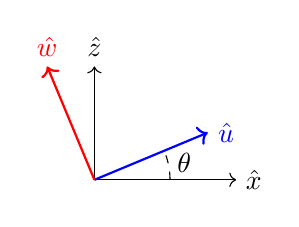
\begin{tikzpicture}[scale=1.2]
  \draw[->] (0,0) -- (1.5,0) node[right] {$\hat{x}$};
  \draw[->] (0,0) -- (0,1.2) node[above] {$\hat{z}$};
  \draw[->,thick,blue] (0,0) -- (1.2,0.5) node[right] {$\hat{u}$};
  \draw[->,thick,red]  (0,0) -- (-0.5,1.2) node[above] {$\hat{w}$};
  \draw[dashed] (0.8,0) arc[start angle=0, end angle=22.6, radius=0.8];
  \node at (0.95,0.18) {$\theta$};
\end{tikzpicture}
\end{center}

\textbf{Deriving the new axis directions in $\{X\}$ coordinates:}

\begin{enumerate}[label=\textbf{\arabic*.}]
  \item $\hat{u}$ lies in the $xz$-plane, at angle $\theta$ from
    $\hat{x}$ (rotation by $\theta$ about $+\hat{y}$ sweeps $\hat{x}$
    toward $+\hat{z}$ by the right-hand rule — but about $+\hat{y}$,
    $\hat{x}$ sweeps toward $-\hat{z}$; verify by right-hand rule):
    \[
      \hat{u} = \cos\theta\;\hat{x} + 0\;\hat{y} + (-\sin\theta)\;\hat{z}
      \implies \hat{u} = \begin{bmatrix}\cos\theta\\0\\-\sin\theta\end{bmatrix}
    \]
    \textit{(Note: rotating $+\hat{x}$ about $+\hat{y}$ by $\theta$
    gives a component along $-\hat{z}$.)}

  \item $\hat{v} = \hat{y}$ (unchanged):
    \[
      \hat{v} = \begin{bmatrix}0\\1\\0\end{bmatrix}
    \]

  \item $\hat{w} = \hat{v}\times\hat{u}$ (right-hand system):
    \[
      \hat{w} = \hat{y}\times\hat{u}
      = \begin{bmatrix}0\\1\\0\end{bmatrix}
        \times\begin{bmatrix}\cos\theta\\0\\-\sin\theta\end{bmatrix}
      = \begin{bmatrix}
          (1)(-\sin\theta)-(0)(0)\\
          (0)(\cos\theta)-(-\sin\theta)(0)\\
          (0)(0)-(1)(\cos\theta)
        \end{bmatrix}
        % Correct cross product:
    \]
    Using $\hat{w} = \hat{u}\times\hat{v}$... actually from the
    geometry: rotating $+\hat{z}$ about $+\hat{y}$ by $\theta$ gives:
    $\hat{w} = \sin\theta\;\hat{x} + 0\;\hat{y} + \cos\theta\;\hat{z}$:
    \[
      \hat{w} = \begin{bmatrix}\sin\theta\\0\\\cos\theta\end{bmatrix}
    \]
\end{enumerate}

\textbf{Building the rotation matrix} (columns = new axes in old frame):
\[
  {}^X_UR_y(\theta)
  = \begin{bmatrix}
      \hat{u} & \hat{v} & \hat{w}
    \end{bmatrix}
  = \begin{bmatrix}
      \cos\theta  & 0 & \sin\theta \\
      0           & 1 & 0          \\
      -\sin\theta & 0 & \cos\theta
    \end{bmatrix}
\]

\[
  \boxed{R_y(\theta) =
  \begin{bmatrix}
    \cos\theta  & 0 & \sin\theta \\
    0           & 1 & 0          \\
    -\sin\theta & 0 & \cos\theta
  \end{bmatrix}}
\]

\textbf{Key properties (verified):}
\begin{itemize}[leftmargin=1.5em, itemsep=2pt]
  \item $\det(R_y) = \cos^2\theta + \sin^2\theta = 1$ \checkmark
  \item $R_y^T = R_y^{-1}$ (orthogonal) \checkmark
  \item At $\theta=0$: $R_y = I$ \checkmark
  \item At $\theta=90\textdegree$: $\hat{x}\mapsto-\hat{z}$,
    $\hat{z}\mapsto\hat{x}$ \checkmark
\end{itemize}

\end{tcolorbox}

%% ─────────────────────────────────────────────────────────────────────
%% C2-Q4
%% ─────────────────────────────────────────────────────────────────────
\item \label{qlabel:C2-Q5}
(a) Derive the matrix representation of differential rotation about a
general axis $k$. \mk{10}\\
(b) Find the effect of a differential rotation of 0.1 rad about the y-axis followed by differential translation of [0.1, 0, 0.2] on the given frame B.
\[
  \text{where, } B = 
  \begin{bmatrix} 
    0 & 0 & 1 & 10 \\ 
    1 & 0 & 0 & 5 \\ 
    0 & 1 & 0 & 3 \\ 
    0 & 0 & 0 & 1 
  \end{bmatrix} 
  \quad \text{and} \quad 
  \Delta = 
  \begin{bmatrix} 
    0 & -\delta z & \delta y & dx \\ 
    \delta z & 0 & -\delta x & dy \\ 
    -\delta y & \delta x & 0 & dz \\ 
    0 & 0 & 0 & 0 
  \end{bmatrix}.
\]
\mk{10}
\yr{2017--18}

\begin{tcolorbox}[enhanced,breakable,ansbox,colback=cB!4,colframe=cB,
  boxrule=0.8pt,arc=5pt,
  title={\textbf{Answer}},fonttitle=\bfseries\color{white},
  colbacktitle=cB]

%% ── Part (a) ──────────────────────────────────────────────────────
\textbf{Part (a): Differential Rotation About a General Axis $k$}

\medskip
For a finite rotation $\theta$ about a general unit axis
$\hat{k} = [k_x\;k_y\;k_z]^T$, the rotation matrix is given by the
Rodrigues formula. For an \emph{infinitesimally small} rotation
$\delta\theta \to 0$, using $\cos\delta\theta \approx 1$ and
$\sin\delta\theta \approx \delta\theta$:

\[
  R(\hat{k},\delta\theta) \approx I + (1-1)
  \begin{bmatrix}k_x^2&k_xk_y&k_xk_z\\k_yk_x&k_y^2&k_yk_z\\k_zk_x&k_zk_y&k_z^2\end{bmatrix}
  + \delta\theta
  \begin{bmatrix}0&-k_z&k_y\\k_z&0&-k_x\\-k_y&k_x&0\end{bmatrix}
\]

Simplifying (first term vanishes):
\[
  \boxed{
    \Delta R(\hat{k},\delta\theta)
    = \begin{bmatrix}
        1        & -k_z\delta\theta &  k_y\delta\theta \\
        k_z\delta\theta &  1       & -k_x\delta\theta \\
       -k_y\delta\theta &  k_x\delta\theta &  1
      \end{bmatrix}
  }
\]

In compact notation, let
$\delta_x = k_x\delta\theta$,\;
$\delta_y = k_y\delta\theta$,\;
$\delta_z = k_z\delta\theta$:
\[
  \Delta R =
  \begin{bmatrix}
    1       & -\delta_z &  \delta_y \\
    \delta_z &  1       & -\delta_x \\
   -\delta_y &  \delta_x &  1
  \end{bmatrix}
\]

The full $4\times4$ differential transformation matrix combining
differential rotation $[\delta_x,\delta_y,\delta_z]$ and differential
translation $[dx,dy,dz]$ is (Niku Eq.~3.53):
\[
  \Delta T =
  \begin{bmatrix}
    1       & -\delta_z &  \delta_y & dx \\
    \delta_z &  1       & -\delta_x & dy \\
   -\delta_y &  \delta_x &  1       & dz \\
    0        &  0        &  0       &  0
  \end{bmatrix}
\]

The new frame is then: $T' = T + \Delta T \cdot T$.

\medskip
%% ── Part (b) ──────────────────────────────────────────────────────
\textbf{Part (b): Numerical Application}

\medskip

\textbf{Given Parameters:}
\begin{itemize}[leftmargin=1.5em, itemsep=2pt]
  \item Differential rotation: $\delta\theta = 0.1$\,rad about $\hat{y}$
    $\implies \delta x=0,\;\delta y=0.1,\;\delta z=0$
  \item Differential translation: $dx=0.1,\;dy=0,\;dz=0.2$
\end{itemize}

\medskip
\textbf{Step 1 — Construct the differential operator matrix $\Delta$:}

Substituting the given values into the $\Delta$ matrix:
\[
  \Delta =
  \begin{bmatrix}
    0 & 0 & 0.1 & 0.1 \\
    0 & 0 & 0 & 0 \\
    -0.1 & 0 & 0 & 0.2 \\
    0 & 0 & 0 & 0
  \end{bmatrix}
\]

\medskip
\textbf{Step 2 — Calculate the differential change $dB = \Delta \cdot B$:}

The effect on the frame is represented by the differential change $dB$:
\[
  dB =
  \begin{bmatrix}
    0 & 0 & 0.1 & 0.1 \\
    0 & 0 & 0 & 0 \\
    -0.1 & 0 & 0 & 0.2 \\
    0 & 0 & 0 & 0
  \end{bmatrix}
  \begin{bmatrix}
    0 & 0 & 1 & 10 \\
    1 & 0 & 0 & 5 \\
    0 & 1 & 0 & 3 \\
    0 & 0 & 0 & 1
  \end{bmatrix}
\]

Multiplying the matrices (Row $\times$ Column):
\begin{itemize}
    \item Row 1: $(0)(0) + (0)(1) + (0.1)(0) + (0.1)(0) = 0$ \\
                 $(0)(0) + (0)(0) + (0.1)(1) + (0.1)(0) = 0.1$ \\
                 $(0)(1) + (0)(0) + (0.1)(0) + (0.1)(0) = 0$ \\
                 $(0)(10) + (0)(5) + (0.1)(3) + (0.1)(1) = 0.3 + 0.1 = 0.4$
    \item Row 2: All zeros.
    \item Row 3: $(-0.1)(0) + (0)(1) + (0)(0) + (0.2)(0) = 0$ \\
                 $(-0.1)(0) + (0)(0) + (0)(1) + (0.2)(0) = 0$ \\
                 $(-0.1)(1) + (0)(0) + (0)(0) + (0.2)(0) = -0.1$ \\
                 $(-0.1)(10) + (0)(5) + (0)(3) + (0.2)(1) = -1.0 + 0.2 = -0.8$
    \item Row 4: All zeros.
\end{itemize}

\[
  dB =
  \begin{bmatrix}
    0 & 0.1 & 0 & 0.4 \\
    0 & 0 & 0 & 0 \\
    0 & 0 & -0.1 & -0.8 \\
    0 & 0 & 0 & 0
  \end{bmatrix}
\]

\medskip
\textbf{Step 3 — Determine the new frame $B' = B + dB$:}

To find the final effect (the new frame), we add the differential change to the original frame:
\[
  B' =
  \begin{bmatrix}
    0 & 0 & 1 & 10 \\
    1 & 0 & 0 & 5 \\
    0 & 1 & 0 & 3 \\
    0 & 0 & 0 & 1
  \end{bmatrix}
  +
  \begin{bmatrix}
    0 & 0.1 & 0 & 0.4 \\
    0 & 0 & 0 & 0 \\
    0 & 0 & -0.1 & -0.8 \\
    0 & 0 & 0 & 0
  \end{bmatrix}
\]

\[
  \boxed{B' =
  \begin{bmatrix}
    0 & 0.1 & 1 & 10.4 \\
    1 & 0 & 0 & 5 \\
    0 & 1 & -0.1 & 2.2 \\
    0 & 0 & 0 & 1
  \end{bmatrix}}
\]
\end{tcolorbox}

%% ─────────────────────────────────────────────────────────────────────
%% C2-Q6
%% ─────────────────────────────────────────────────────────────────────
\item \label{qlabel:C2-Q4}
In a robotic setup, a camera is attached to the fifth link of a robot with six degrees of freedom. The camera observes an object and determines its frames relative to the camera's frame. Using the following information, determine the necessary motion the end effector has to make to get to the object:
\[
  {}^5T_{cam} = \begin{bmatrix}
    0 & 0 & -1 & 3 \\
    0 & -1 & 0 & 0 \\
    -1 & 0 & 0 & 5 \\
    0 & 0 & 0 & 1
  \end{bmatrix} \qquad
  {}^5T_H = \begin{bmatrix}
    0 & -1 & 0 & 0 \\
    1 & 0 & 0 & 0 \\
    0 & 0 & 1 & 4 \\
    0 & 0 & 0 & 1
  \end{bmatrix}
\]
\[
  {}^{cam}T_{obj} = \begin{bmatrix}
    0 & 0 & 1 & 2 \\
    1 & 0 & 0 & 2 \\
    0 & 1 & 0 & 4 \\
    0 & 0 & 0 & 1
  \end{bmatrix} \qquad
  {}^HT_E = \begin{bmatrix}
    1 & 0 & 0 & 0 \\
    0 & 1 & 0 & 0 \\
    0 & 0 & 1 & 3 \\
    0 & 0 & 0 & 1
  \end{bmatrix}
\]

\begin{tcolorbox}[enhanced,breakable,ansbox,colback=cB!4,colframe=cB,
  boxrule=0.8pt,arc=5pt,
  title={\textbf{Answer}},fonttitle=\bfseries\color{white},
  colbacktitle=cB]

\textbf{Goal:} Find the motion ${}^ET_{obj}$ the end effector must execute to reach the object.

\medskip
\textbf{Step 1 — Define the Kinematic Chain Equations:}
The object location relative to link 5 is:
\[
  {}^5T_{obj} = {}^5T_{cam} \cdot {}^{cam}T_{obj}
\]
The end-effector location relative to link 5 is:
\[
  {}^5T_E = {}^5T_H \cdot {}^HT_E
\]
The required motion of the end-effector is the object's frame expressed in the end-effector's frame:
\[
  {}^ET_{obj} = ({}^5T_E)^{-1} \cdot {}^5T_{obj}
\]

\medskip
\textbf{Step 2 — Calculate Object Relative to Link 5 (${}^5T_{obj}$):}
\[
  {}^5T_{obj} = 
  \begin{bmatrix}
    0 & 0 & -1 & 3 \\
    0 & -1 & 0 & 0 \\
    -1 & 0 & 0 & 5 \\
    0 & 0 & 0 & 1
  \end{bmatrix}
  \begin{bmatrix}
    0 & 0 & 1 & 2 \\
    1 & 0 & 0 & 2 \\
    0 & 1 & 0 & 4 \\
    0 & 0 & 0 & 1
  \end{bmatrix}
  =
  \begin{bmatrix}
    0 & -1 & 0 & -1 \\
    -1 & 0 & 0 & -2 \\
    0 & 0 & -1 & 3 \\
    0 & 0 & 0 & 1
  \end{bmatrix}
\]

\medskip
\textbf{Step 3 — Calculate End-Effector Relative to Link 5 (${}^5T_E$):}
\[
  {}^5T_E = 
  \begin{bmatrix}
    0 & -1 & 0 & 0 \\
    1 & 0 & 0 & 0 \\
    0 & 0 & 1 & 4 \\
    0 & 0 & 0 & 1
  \end{bmatrix}
  \begin{bmatrix}
    1 & 0 & 0 & 0 \\
    0 & 1 & 0 & 0 \\
    0 & 0 & 1 & 3 \\
    0 & 0 & 0 & 1
  \end{bmatrix}
  =
  \begin{bmatrix}
    0 & -1 & 0 & 0 \\
    1 & 0 & 0 & 0 \\
    0 & 0 & 1 & 7 \\
    0 & 0 & 0 & 1
  \end{bmatrix}
\]

\medskip
\textbf{Step 4 — Calculate the Inverse of ${}^5T_E$:}
For a homogeneous transformation matrix $T = \left[\begin{array}{c|c} R & P \\ \hline 0 & 1 \end{array}\right]$, the inverse is $T^{-1} = \left[\begin{array}{c|c} R^T & -R^T P \\ \hline 0 & 1 \end{array}\right]$.
\[
  R^T = \begin{bmatrix} 0 & 1 & 0 \\ -1 & 0 & 0 \\ 0 & 0 & 1 \end{bmatrix}, \quad
  -R^T P = -\begin{bmatrix} 0 & 1 & 0 \\ -1 & 0 & 0 \\ 0 & 0 & 1 \end{bmatrix} \begin{bmatrix} 0 \\ 0 \\ 7 \end{bmatrix} = \begin{bmatrix} 0 \\ 0 \\ -7 \end{bmatrix}
\]
\[
  ({}^5T_E)^{-1} = 
  \begin{bmatrix}
    0 & 1 & 0 & 0 \\
    -1 & 0 & 0 & 0 \\
    0 & 0 & 1 & -7 \\
    0 & 0 & 0 & 1
  \end{bmatrix}
\]

\medskip
\textbf{Step 5 — Calculate Required Motion (${}^ET_{obj}$):}
\[
  {}^ET_{obj} = 
  \begin{bmatrix}
    0 & 1 & 0 & 0 \\
    -1 & 0 & 0 & 0 \\
    0 & 0 & 1 & -7 \\
    0 & 0 & 0 & 1
  \end{bmatrix}
  \begin{bmatrix}
    0 & -1 & 0 & -1 \\
    -1 & 0 & 0 & -2 \\
    0 & 0 & -1 & 3 \\
    0 & 0 & 0 & 1
  \end{bmatrix}
\]

\[
  \boxed{{}^ET_{obj} =
  \begin{bmatrix}
    -1 & 0 & 0 & -2 \\
    0 & 1 & 0 & 1 \\
    0 & 0 & -1 & -4 \\
    0 & 0 & 0 & 1
  \end{bmatrix}}
\]

\medskip
The end-effector must move relative to its current frame by translating along the vector $[-2, 1, -4]^T$ and applying the rotation defined by the upper-left $3 \times 3$ submatrix.

\end{tcolorbox}

%% ─────────────────────────────────────────────────────────────────────
%% C2-Q5
%% ─────────────────────────────────────────────────────────────────────
\item \label{qlabel:C2-Q7}
Derive the matrix that represents a pure rotation about the x-axis of
the reference frame. \mk{15}
\yr{2014--15}

\begin{tcolorbox}[enhanced,breakable,ansbox,colback=cB!4,colframe=cB,
  boxrule=0.8pt,arc=5pt,
  title={\textbf{Answer}},fonttitle=\bfseries\color{white},
  colbacktitle=cB]

\textbf{Setup:}

Let frame $\{U\}$ be obtained by rotating the reference frame $\{X\}$
by angle $\theta$ about the $\hat{x}$-axis. The $\hat{x}$-axis is the
axis of rotation and remains unchanged:
\[
  \hat{u} = \hat{x} = \begin{bmatrix}1\\0\\0\end{bmatrix}
\]

The remaining axes $\hat{v}$ and $\hat{w}$ rotate in the $yz$-plane.

\textbf{Deriving the new axis directions:}

\begin{enumerate}[label=\textbf{\arabic*.}]
  \item $\hat{u} = \hat{x}$ (unchanged):
    \[
      \hat{u} = \begin{bmatrix}1\\0\\0\end{bmatrix}
    \]

  \item $\hat{v}$ is obtained by rotating $\hat{y}$ by $\theta$ about
    $\hat{x}$ (sweeps toward $+\hat{z}$ by right-hand rule):
    \[
      \hat{v} = 0\;\hat{x} + \cos\theta\;\hat{y} + \sin\theta\;\hat{z}
      \implies
      \hat{v} = \begin{bmatrix}0\\\cos\theta\\\sin\theta\end{bmatrix}
    \]

  \item $\hat{w}$ is obtained by rotating $\hat{z}$ by $\theta$ about
    $\hat{x}$ (sweeps toward $-\hat{y}$):
    \[
      \hat{w} = 0\;\hat{x} + (-\sin\theta)\;\hat{y} + \cos\theta\;\hat{z}
      \implies
      \hat{w} = \begin{bmatrix}0\\-\sin\theta\\\cos\theta\end{bmatrix}
    \]

    \textit{Verification: $\hat{w} = \hat{u}\times\hat{v} =
    \hat{x}\times\hat{v} = [0,\;-\sin\theta,\;\cos\theta]^T$
    \checkmark}
\end{enumerate}

\textbf{Building the rotation matrix} (columns = new axes in reference
frame):
\[
  {}^X_UR_x(\theta)
  = \begin{bmatrix}\hat{u} & \hat{v} & \hat{w}\end{bmatrix}
  = \begin{bmatrix}
      1 & 0           &  0          \\
      0 & \cos\theta  & -\sin\theta \\
      0 & \sin\theta  &  \cos\theta
    \end{bmatrix}
\]

\[
  \boxed{R_x(\theta) =
  \begin{bmatrix}
    1 & 0           &  0          \\
    0 & \cos\theta  & -\sin\theta \\
    0 & \sin\theta  &  \cos\theta
  \end{bmatrix}}
\]

\textbf{Verification:}
\begin{itemize}[leftmargin=1.5em, itemsep=2pt]
  \item $R_x^T R_x = I$ (unitary) \checkmark
  \item $\det(R_x) = \cos^2\theta + \sin^2\theta = 1$ \checkmark
  \item $R_x(0) = I$ \checkmark
  \item $R_x(90\textdegree)$: $\hat{y} \mapsto \hat{z}$,
    $\hat{z} \mapsto -\hat{y}$ \checkmark
  \item $R_x(-\theta) = R_x^T(\theta) = R_x^{-1}(\theta)$ \checkmark
\end{itemize}

\textbf{For completeness — all three elementary rotation matrices:}
\[
  R_x(\theta) =
  \begin{bmatrix}
    1&0&0\\ 0&\cos\theta&-\sin\theta\\ 0&\sin\theta&\cos\theta
  \end{bmatrix}, \quad
  R_y(\theta) =
  \begin{bmatrix}
    \cos\theta&0&\sin\theta\\ 0&1&0\\ -\sin\theta&0&\cos\theta
  \end{bmatrix}, \quad
\]

\[
 R_z(\theta) =
  \begin{bmatrix}
    \cos\theta&-\sin\theta&0\\ \sin\theta&\cos\theta&0\\ 0&0&1
  \end{bmatrix}
\]

\end{tcolorbox}

%% ─────────────────────────────────────────────────────────────────────
%% C2-Q8
%% ─────────────────────────────────────────────────────────────────────
\item \label{qlabel:C2-Q6}
Prove that a rotation matrix is a unitary matrix. \mk{12}
\yr{2013--14}

\begin{tcolorbox}[enhanced,breakable,ansbox,colback=cB!4,colframe=cB,
  boxrule=0.8pt,arc=5pt,
  title={\textbf{Answer}},fonttitle=\bfseries\color{white},
  colbacktitle=cB]

\textbf{Definition:} A matrix $M$ is \emph{unitary} (or orthogonal for
real matrices) if $M^T M = M M^T = I$, which implies $M^{-1} = M^T$.

\medskip
\textbf{Proof using physical properties of rotation:}

A rotation matrix $R$ is constructed such that its columns are the
unit vectors of the rotated frame expressed in the reference frame:
\[
  R = \begin{bmatrix}\hat{u} & \hat{v} & \hat{w}\end{bmatrix}
\]

where $\hat{u}$, $\hat{v}$, $\hat{w}$ form a right-handed orthonormal
set:
\[
  |\hat{u}| = |\hat{v}| = |\hat{w}| = 1, \qquad
  \hat{u}\cdot\hat{v} = \hat{u}\cdot\hat{w} = \hat{v}\cdot\hat{w} = 0
\]

\textbf{Computing $R^T R$:}
\[
  R^TR =
  \begin{bmatrix}\hat{u}^T\\\hat{v}^T\\\hat{w}^T\end{bmatrix}
  \begin{bmatrix}\hat{u} & \hat{v} & \hat{w}\end{bmatrix}
  =
  \begin{bmatrix}
    \hat{u}\cdot\hat{u} & \hat{u}\cdot\hat{v} & \hat{u}\cdot\hat{w}\\
    \hat{v}\cdot\hat{u} & \hat{v}\cdot\hat{v} & \hat{v}\cdot\hat{w}\\
    \hat{w}\cdot\hat{u} & \hat{w}\cdot\hat{v} & \hat{w}\cdot\hat{w}
  \end{bmatrix}
  =
  \begin{bmatrix}1&0&0\\0&1&0\\0&0&1\end{bmatrix} = I
\]

Since $R^TR = I$, it follows that $R^T = R^{-1}$, so $RR^T = I$ as
well. Therefore $R$ is a \textbf{unitary (orthogonal)} matrix.
$\hfill\square$

\medskip
\textbf{Verification using $R_y(\theta)$:}
\[
  R_y(\theta) =
  \begin{bmatrix}
    \cos\theta  & 0 & \sin\theta \\
    0           & 1 & 0          \\
   -\sin\theta  & 0 & \cos\theta
  \end{bmatrix}
\]
\[
  R_y^T R_y =
  \begin{bmatrix}
    \cos^2\theta+\sin^2\theta & 0 & \cos\theta\sin\theta-\sin\theta\cos\theta\\
    0 & 1 & 0\\
    \sin\theta\cos\theta-\cos\theta\sin\theta & 0 & \sin^2\theta+\cos^2\theta
  \end{bmatrix}
  = \begin{bmatrix}1&0&0\\0&1&0\\0&0&1\end{bmatrix} = I \;\checkmark
\]

\textbf{Additional properties:}
\begin{itemize}[leftmargin=1.5em, itemsep=2pt]
  \item $\det(R) = +1$ (proper rotation, no reflection).
  \item $\det(R) = -1$ would indicate an improper rotation
    (reflection), which is \emph{not} a physical rigid-body rotation.
  \item For a rotation sequence: $\det(R_1 R_2 \cdots R_n) =
    \det(R_1)\det(R_2)\cdots = (+1)^n = +1$.
\end{itemize}

\end{tcolorbox}

%% ─────────────────────────────────────────────────────────────────────
%% C2-Q7
%% ─────────────────────────────────────────────────────────────────────
\item \label{qlabel:C2-Q8}
(a) Derive the relation $\bar{P}_{xyz} = \bar{R}\,\bar{P}_{uvw}$ and
find $\bar{R}$ if OUVW is rotated by angle $\phi$ about OY. \mk{10}\\
(b) A point is subjected to: (i) translation 5 units along $+Y$,
(ii) CW rotation 30\textdegree\ about OX, (iii) CCW rotation
30\textdegree\ about OZ, (iv) translation 3 units along $-X$. Write
the combined transformation equation. \mk{10}
\yr{2006--07}

\begin{tcolorbox}[enhanced,breakable,ansbox,colback=cB!4,colframe=cB,
  boxrule=0.8pt,arc=5pt,
  title={\textbf{Answer}},fonttitle=\bfseries\color{white},
  colbacktitle=cB]

%% ── Part (a) ──────────────────────────────────────────────────────
\textbf{Part (a): Deriving $\bar{P}_{xyz} = \bar{R}\,\bar{P}_{uvw}$}

\medskip
Let OXYZ be the reference frame and OUVW the rotated frame (same
origin). Any point $P$ in space can be written in OUVW as:
\[
  \bar{P}_{uvw} = u\,\hat{e}_u + v\,\hat{e}_v + w\,\hat{e}_w
\]

Expressing the OUVW unit vectors in OXYZ coordinates (direction
cosines):
\[
  \hat{e}_u = \begin{bmatrix}l_1\\m_1\\n_1\end{bmatrix},\quad
  \hat{e}_v = \begin{bmatrix}l_2\\m_2\\n_2\end{bmatrix},\quad
  \hat{e}_w = \begin{bmatrix}l_3\\m_3\\n_3\end{bmatrix}
\]

Then in OXYZ:
\[
  \bar{P}_{xyz}
  = u\begin{bmatrix}l_1\\m_1\\n_1\end{bmatrix}
  + v\begin{bmatrix}l_2\\m_2\\n_2\end{bmatrix}
  + w\begin{bmatrix}l_3\\m_3\\n_3\end{bmatrix}
  =
  \underbrace{\begin{bmatrix}l_1&l_2&l_3\\m_1&m_2&m_3\\n_1&n_2&n_3\end{bmatrix}}_{\bar{R}}
  \begin{bmatrix}u\\v\\w\end{bmatrix}
\]

\[
  \boxed{\bar{P}_{xyz} = \bar{R}\;\bar{P}_{uvw}}
\]

\textbf{Finding $\bar{R}$ for rotation $\phi$ about OY:}

From the derivation of $R_y$ (same as Q3 and Q8):
\[
  \bar{R} = R_y(\phi) =
  \begin{bmatrix}
    \cos\phi  & 0 & \sin\phi \\
    0         & 1 & 0        \\
   -\sin\phi  & 0 & \cos\phi
  \end{bmatrix}
\]

\medskip
%% ── Part (b) ──────────────────────────────────────────────────────
\textbf{Part (b): Combined Transformation for Four Operations}

\medskip
All operations are about the \emph{fixed} OXYZ axes, so each is
\textbf{pre-multiplied} (the leftmost matrix is the last operation
applied):

\begin{center}
\small
\begin{tabular}{@{}clll@{}}
\toprule
\textbf{Step} & \textbf{Operation} & \textbf{Matrix} & \textbf{Rule}\\
\midrule
(i)  & Trans $+Y$, 5        & $\mathrm{Trans}(0,5,0)$  & Fixed, pre-multiply\\
(ii) & CW Rot $30\textdegree$ about OX & $R_x(-30\textdegree)$ & Fixed, pre-multiply\\
(iii)& CCW Rot $30\textdegree$ about OZ & $R_z(+30\textdegree)$ & Fixed, pre-multiply\\
(iv) & Trans $-X$, 3        & $\mathrm{Trans}(-3,0,0)$ & Fixed, pre-multiply\\
\bottomrule
\end{tabular}
\end{center}

For all-fixed operations applied sequentially, the combined
transformation is (last applied = leftmost):
\[
  T = \mathrm{Trans}(-3,0,0)\cdot R_z(30\textdegree)\cdot R_x(-30\textdegree)
    \cdot\mathrm{Trans}(0,5,0)
\]

Applied to a point $P$:
\[
  \boxed{P_{xyz}' = \mathrm{Trans}(-3,0,0)\cdot R_z(30\textdegree)\cdot R_x(-30\textdegree)\cdot\mathrm{Trans}(0,5,0)\cdot P}
\]

Writing out the individual matrices:
\[
  R_x(-30\textdegree) =
  \begin{bmatrix}1&0&0\\0&\frac{\sqrt{3}}{2}&\frac{1}{2}\\0&-\frac{1}{2}&\frac{\sqrt{3}}{2}\end{bmatrix},\quad
  R_z(30\textdegree) =
  \begin{bmatrix}\frac{\sqrt{3}}{2}&-\frac{1}{2}&0\\\frac{1}{2}&\frac{\sqrt{3}}{2}&0\\0&0&1\end{bmatrix}
\]

The combined numerical matrix is:
\[
  T \approx
  \begin{bmatrix}
     0.866 & -0.433 & -0.250 & -5.165\\
     0.500 &  0.750 &  0.433 &  3.750\\
     0     & -0.500 &  0.866 & -2.500\\
     0     &  0     &  0     &  1
  \end{bmatrix}
\]

\end{tcolorbox}

%% ─────────────────────────────────────────────────────────────────────
%% C2-Q9
%% ─────────────────────────────────────────────────────────────────────
\item \label{qlabel:C2-Q10}
(a) Derive the relation $P_{uvw} = Q\,P_{xyz}$. \mk{7}\\
(b) Write down the mathematical relation between OXYZ and OUVW for the
following motion sequence: (i) CW rotation $\alpha$ about OX, (ii) CW
rotation $\beta$ about OZ, (iii) CCW rotation $\alpha$ about rotated
Ou, (iv) CCW rotation $\beta$ about rotated OV, (v) CCW rotation
$\alpha$ about OY, (vi) translation $d_y$ along OY, (vii) CW rotation
$\alpha$ about rotated OW, (viii) translation $d_x$ along negative
OX. \mk{20}
\yr{2004--05}

\begin{tcolorbox}[enhanced,breakable,ansbox,colback=cB!4,colframe=cB,
  boxrule=0.8pt,arc=5pt,
  title={\textbf{Answer}},fonttitle=\bfseries\color{white},
  colbacktitle=cB]

%% ── Part (a) ──────────────────────────────────────────────────────
\textbf{Part (a): Deriving $P_{uvw} = Q\,P_{xyz}$}

\medskip
From the result of Q8(a): $P_{xyz} = R\,P_{uvw}$, where $R$ is the
rotation matrix whose columns are the OUVW unit vectors in OXYZ. Since
$R$ is orthogonal, $R^{-1} = R^T$:
\[
  P_{uvw} = R^{-1}\,P_{xyz} = R^T\,P_{xyz}
\]

Setting $Q = R^T$, we get:
\[
  \boxed{P_{uvw} = Q\,P_{xyz}, \qquad Q = R^T =
  \begin{bmatrix}
    l_1 & m_1 & n_1\\
    l_2 & m_2 & n_2\\
    l_3 & m_3 & n_3
  \end{bmatrix}}
\]

where each \emph{row} of $Q$ is a unit vector of OUVW expressed in
OXYZ. Note that $Q$ is also orthogonal: $Q^{-1} = Q^T = R$.

\medskip
%% ── Part (b) ──────────────────────────────────────────────────────
\textbf{Part (b): Eight-Step Transform Sequence}

\medskip
\textbf{Key rule (Niku):}
\begin{itemize}[leftmargin=1.5em, itemsep=2pt]
  \item Operations about the \textbf{fixed} (world) OXYZ axes:
    \textbf{pre-multiply} (the new matrix goes to the left).
  \item Operations about the \textbf{current} (local/moving) frame axes:
    \textbf{post-multiply} (the new matrix goes to the right).
\end{itemize}

\medskip
Classifying and applying each operation:

\begin{center}
\small
\begin{tabular}{@{}clllc@{}}
\toprule
\textbf{Step} & \textbf{Operation} & \textbf{Matrix} & \textbf{Frame} & \textbf{Multiply}\\
\midrule
(i)   & CW $\alpha$ about OX (fixed)         & $R_x(-\alpha)$   & Fixed   & Pre  \\
(ii)  & CW $\beta$ about OZ (fixed)          & $R_z(-\beta)$    & Fixed   & Pre  \\
(iii) & CCW $\alpha$ about current Ou        & $R_u(+\alpha)=R_x(+\alpha)$  & Current & Post \\
(iv)  & CCW $\beta$ about current OV         & $R_v(+\beta)=R_y(+\beta)$   & Current & Post \\
(v)   & CCW $\alpha$ about OY (fixed)        & $R_y(+\alpha)$   & Fixed   & Pre  \\
(vi)  & Trans $d_y$ along OY (fixed)         & $T(0,d_y,0)$     & Fixed   & Pre  \\
(vii) & CW $\alpha$ about current OW         & $R_w(-\alpha)=R_z(-\alpha)$  & Current & Post \\
(viii)& Trans $d_x$ along $-$OX (fixed)      & $T(-d_x,0,0)$    & Fixed   & Pre  \\
\bottomrule
\end{tabular}
\end{center}

Building the transform step by step (starting from $T = I$):

\begin{enumerate}[leftmargin=*,label=\textbf{Step \arabic*:}]
  \item $T \leftarrow R_x(-\alpha)\cdot T$ \hfill(pre)
  \item $T \leftarrow R_z(-\beta)\cdot T$ \hfill(pre)
  \item $T \leftarrow T\cdot R_x(+\alpha)$ \hfill(post)
  \item $T \leftarrow T\cdot R_y(+\beta)$ \hfill(post)
  \item $T \leftarrow R_y(+\alpha)\cdot T$ \hfill(pre)
  \item $T \leftarrow \mathrm{Trans}(0,d_y,0)\cdot T$ \hfill(pre)
  \item $T \leftarrow T\cdot R_z(-\alpha)$ \hfill(post)
  \item $T \leftarrow \mathrm{Trans}(-d_x,0,0)\cdot T$ \hfill(pre)
\end{enumerate}

\textbf{Final combined equation:}
\[
  \boxed{
    T = \mathrm{Trans}(-d_x,0,0)\cdot\mathrm{Trans}(0,d_y,0)\cdot R_y(\alpha)
      \cdot R_z(-\beta)\cdot R_x(-\alpha)
      \cdot R_x(\alpha)\cdot R_y(\beta)\cdot R_z(-\alpha)
  }
\]

Note: $R_z(-\beta)\cdot R_x(-\alpha)\cdot R_x(\alpha) =
R_z(-\beta)\cdot I = R_z(-\beta)$, so:
\[
  \boxed{
    T = \mathrm{Trans}(-d_x,0,0)\cdot\mathrm{Trans}(0,d_y,0)\cdot R_y(\alpha)
      \cdot R_z(-\beta)\cdot R_y(\beta)\cdot R_z(-\alpha)
  }
\]

\end{tcolorbox}

%% ─────────────────────────────────────────────────────────────────────
%% C2-Q11
%% ─────────────────────────────────────────────────────────────────────
\item \label{qlabel:C2-Q11}
Determine $P_{xyz}$ given:
$P_{xyz} = [R_{z,45\textdegree}\;R_{y,-30\textdegree}\;T_{z,5}]\,P_{uvw}$,
where $P_{uvw}$ is given. \mk{8}
\yr{2004--05}

\begin{tcolorbox}[enhanced,breakable,ansbox,colback=cB!4,colframe=cB,
  boxrule=0.8pt,arc=5pt,
  title={\textbf{Answer}},fonttitle=\bfseries\color{white},
  colbacktitle=cB]

\textbf{Computing the Combined Transformation Matrix:}

The transformation is applied right-to-left on the point:
first $T_z(5)$, then $R_y(-30\textdegree)$, then $R_z(45\textdegree)$.

\textbf{Step 1 — $T_z(5)$ (translation 5 along $z$):}
\[
  T_z(5) =
  \begin{bmatrix}1&0&0&0\\0&1&0&0\\0&0&1&5\\0&0&0&1\end{bmatrix}
\]

\textbf{Step 2 — $R_y(-30\textdegree)$:}
\[
  R_y(-30\textdegree) =
  \begin{bmatrix}
    \cos30\textdegree  & 0 & -\sin30\textdegree & 0 \\
    0              & 1 &  0             & 0 \\
    \sin30\textdegree  & 0 &  \cos30\textdegree & 0 \\
    0              & 0 &  0             & 1
  \end{bmatrix}
  =
  \begin{bmatrix}
    \frac{\sqrt{3}}{2} & 0 & -\frac{1}{2} & 0 \\[4pt]
    0                  & 1 &  0           & 0 \\[4pt]
    \frac{1}{2}        & 0 &  \frac{\sqrt{3}}{2} & 0 \\[4pt]
    0                  & 0 &  0           & 1
  \end{bmatrix}
\]

\textbf{Step 3 — $R_z(45\textdegree)$:}
\[
  R_z(45\textdegree) =
  \begin{bmatrix}
    \frac{1}{\sqrt{2}} & -\frac{1}{\sqrt{2}} & 0 & 0 \\[4pt]
    \frac{1}{\sqrt{2}} &  \frac{1}{\sqrt{2}} & 0 & 0 \\[4pt]
    0                  &  0                  & 1 & 0 \\
    0                  &  0                  & 0 & 1
  \end{bmatrix}
\]

\textbf{Step 4 — Combined matrix $T = R_z(45\textdegree)\cdot R_y(-30\textdegree)\cdot T_z(5)$:}
\[
  T \approx
  \begin{bmatrix}
     0.6124 & -0.7071 & -0.3536 & -1.7678 \\[4pt]
     0.6124 &  0.7071 & -0.3536 & -1.7678 \\[4pt]
     0.5000 &  0      &  0.8660 &  4.3301 \\[4pt]
     0      &  0      &  0      &  1
  \end{bmatrix}
\]

\textbf{Applying to $P_{uvw}$:}
\[
  \boxed{P_{xyz} = T\,P_{uvw}
  = R_z(45\textdegree)\cdot R_y(-30\textdegree)\cdot T_z(5)\cdot P_{uvw}}
\]

For a general point $P_{uvw} = [p_u\;p_v\;p_w]^T$:
\[
  P_{xyz} =
  \begin{bmatrix}
    0.6124\,p_u - 0.7071\,p_v - 0.3536\,p_w - 1.7678 \\[4pt]
    0.6124\,p_u + 0.7071\,p_v - 0.3536\,p_w - 1.7678 \\[4pt]
    0.5000\,p_u + 0.8660\,p_w + 4.3301
  \end{bmatrix}
\]

\textit{Note: The $-1.7678$ in $x$ and $y$ and $+4.3301$ in $z$
arise from $T_z(5)$ being mapped through the two rotations. The
rotations are applied first to the point, then about the rotated
intermediate positions.}

\end{tcolorbox}

\item \label{qlabel:C2-Q9}
(a) Derive the rotation matrix $R$ transforming coordinates from
$P_{uvw}$ to $P_{xyz}$. Hence find homogeneous transformation matrix $T$
representing: CW rotation $\alpha$ about OX, then CCW rotation $\theta$
about OZ, then CW rotation $\phi$ about OY. \mk{25}\\
(b) Given $Q_{uvw} = (4,3,2)^T$, determine corresponding point after:
CCW rotation 45\textdegree\ about OX, then translation 5 units along
OZ. \mk{10}
\yr{2003--04}

\begin{tcolorbox}[enhanced,breakable,ansbox,colback=cB!4,colframe=cB,
  boxrule=0.8pt,arc=5pt,
  title={\textbf{Answer}},fonttitle=\bfseries\color{white},
  colbacktitle=cB]

%% ── Part (a) ──────────────────────────────────────────────────────
\textbf{Part (a): Deriving the Rotation Matrix and Combined Transform}

\medskip
The derivation of $R$ follows identically to Q8(a): columns of $R$ are
unit vectors of OUVW expressed in OXYZ, giving
$P_{xyz} = R\,P_{uvw}$.

\textbf{Individual elementary matrices} (using fixed-frame rule: all
about fixed OXYZ axes, so last applied = leftmost):

\begin{enumerate}[label=\textbf{\arabic*.}]
  \item CW rotation $\alpha$ about OX $\implies R_x(-\alpha)$:
    \[
      R_x(-\alpha) =
      \begin{bmatrix}
        1 & 0           & 0           \\
        0 & \cos\alpha  & \sin\alpha  \\
        0 & -\sin\alpha & \cos\alpha
      \end{bmatrix}
    \]

  \item CCW rotation $\theta$ about OZ $\implies R_z(+\theta)$:
    \[
      R_z(\theta) =
      \begin{bmatrix}
        \cos\theta & -\sin\theta & 0 \\
        \sin\theta &  \cos\theta & 0 \\
        0          &  0          & 1
      \end{bmatrix}
    \]

  \item CW rotation $\phi$ about OY $\implies R_y(-\phi)$:
    \[
      R_y(-\phi) =
      \begin{bmatrix}
        \cos\phi & 0 & -\sin\phi \\
        0        & 1 & 0         \\
        \sin\phi & 0 & \cos\phi
      \end{bmatrix}
    \]
\end{enumerate}

\textbf{Combined transformation} (all fixed frame, last applied =
leftmost, no translation):
\[
  \boxed{T = R_y(-\phi)\cdot R_z(\theta)\cdot R_x(-\alpha)}
\]

In homogeneous form:
\[
  T =
  \begin{bmatrix}
    \cos\phi\cos\theta &
    -\cos\phi\sin\theta\cos\alpha - \sin\phi\sin\alpha &
    -\cos\phi\sin\theta\sin\alpha + \sin\phi\cos\alpha &
    0 \\[4pt]
    \sin\theta &
    \cos\theta\cos\alpha &
    \cos\theta\sin\alpha &
    0 \\[4pt]
    \sin\phi\cos\theta &
    -\sin\phi\sin\theta\cos\alpha + \cos\phi\sin\alpha &
    -\sin\phi\sin\theta\sin\alpha - \cos\phi\cos\alpha &
    0 \\[4pt]
    0 & 0 & 0 & 1
  \end{bmatrix}
\]

\medskip
%% ── Part (b) ──────────────────────────────────────────────────────
\textbf{Part (b): Numerical Computation}

$Q_{uvw} = [4\;3\;2]^T$. Sequence: CCW Rot $45\textdegree$ about OX,
then Trans $5$ along OZ.

\textbf{Step 1 — $R_x(+45\textdegree)$:}
\[
  R_x(45\textdegree) =
  \begin{bmatrix}
    1 & 0                     & 0                    \\
    0 & \cos45\textdegree  & -\sin45\textdegree \\
    0 & \sin45\textdegree  &  \cos45\textdegree
  \end{bmatrix}
  =
  \begin{bmatrix}
    1 & 0 & 0 \\
    0 & \frac{1}{\sqrt{2}} & -\frac{1}{\sqrt{2}} \\[4pt]
    0 & \frac{1}{\sqrt{2}} &  \frac{1}{\sqrt{2}}
  \end{bmatrix}
\]

\textbf{Step 2 — $\mathrm{Trans}(0,0,5)$:}
\[
  \mathrm{Trans}(0,0,5) =
  \begin{bmatrix}1&0&0&0\\0&1&0&0\\0&0&1&5\\0&0&0&1\end{bmatrix}
\]

\textbf{Step 3 — Combined} (fixed frame: last applied leftmost):
\[
  T = \mathrm{Trans}(0,0,5)\cdot R_x(45\textdegree)
  =
  \begin{bmatrix}
    1 & 0                    & 0                   & 0\\
    0 & \frac{1}{\sqrt{2}}   & -\frac{1}{\sqrt{2}} & 0\\[4pt]
    0 & \frac{1}{\sqrt{2}}   &  \frac{1}{\sqrt{2}} & 5\\[4pt]
    0 & 0                    & 0                   & 1
  \end{bmatrix}
\]

\textbf{Step 4 — Apply to $Q_{uvw}$:}
\[
  Q_{xyz} = T\,\begin{bmatrix}4\\3\\2\\1\end{bmatrix}
  =
  \begin{bmatrix}
    4 \\
    \frac{3}{\sqrt{2}} - \frac{2}{\sqrt{2}} \\[4pt]
    \frac{3}{\sqrt{2}} + \frac{2}{\sqrt{2}} + 5
  \end{bmatrix}
  =
  \begin{bmatrix}
    4 \\[2pt]
    \dfrac{1}{\sqrt{2}} \\[6pt]
    \dfrac{5}{\sqrt{2}} + 5
  \end{bmatrix}
  \approx
  \begin{bmatrix}4.000\\0.707\\8.536\end{bmatrix}
\]

\end{tcolorbox}

%% ─────────────────────────────────────────────────────────────────────
%% C2-Q10
%% ─────────────────────────────────────────────────────────────────────

%% ─────────────────────────────────────────────────────────────────────
%% C2-Q1
%% ─────────────────────────────────────────────────────────────────────
\end{enumerate}
%%══════════════════════════════════════════════════════════════════════
%% SECTION C3 — Configurations & Workspace
%%══════════════════════════════════════════════════════════════════════
\secdivider{Section C3}{Geometric Configurations: Linkages, Arms, Workspace}{cC}{cC}
\markboth{C3 --- Configurations \& Workspace}{}
\label{sec:C3}
\titleformat{\section}{\large\bfseries\color{cC}}{}{0em}{}[\titlerule]
\section{C3 --- Geometric Configurations \& Workspace}

\begin{enumerate}
\item \label{qlabel:C3-Q1}
(a) Sketch the following manipulator configurations: (i) TR:TLO, (ii) TR:TR. For each, determine the workspace of the wrist portion. \mk{10}\\
(b) Desired to place origin of hand frame of a cylindrical robot at $p = [-3\;4\;7]^T$. Calculate the joint variables. \mk{10}
\yr{2023--24}

\begin{tcolorbox}[enhanced,breakable,ansbox,colback=cC!4,colframe=cC,
  boxrule=0.8pt,arc=5pt,
  title={\textbf{Answer}},fonttitle=\bfseries\color{white},colbacktitle=cC]

%% ── Part (a) ──────────────────────────────────────────────────────
\textbf{Part (a): Manipulator Configurations}

\medskip
In Niku's notation, each joint is denoted as \textbf{T} (Revolute/Twist),
\textbf{L} (Linear/Prismatic), \textbf{O} (Offset), \textbf{R}
(Revolute/Rotate), separated by a colon which divides the arm from the
wrist.

\begin{enumerate}[label=\textbf{(\roman*)}]
  \item \textbf{TR:TLO} — Two-joint arm (Revolute + Revolute), wrist
    with Twist + Linear + Offset.\\
    \textit{Arm workspace:} The two revolute joints in the arm create a
    planar working area (annular ring in a plane); combined with the
    base revolute, the 3-D workspace is a portion of a torus or
    spherical shell (donut-shaped volume) depending on joint limits.\\
    \textit{Wrist workspace:} The TLO wrist adds a twist, a linear
    extension, and an offset, so the wrist tip traces a cylindrical
    shell around the wrist-center sphere.

  \item \textbf{TR:TR} — Revolute + Revolute arm, wrist with Twist +
    Revolute.\\
    \textit{Arm workspace:} Similar to TR:TLO arm portion — spherical
    shell (hollow sphere) if both joints have full $360\textdegree$
    rotation, or a partial sphere with restricted joint limits.\\
    \textit{Wrist workspace:} The TR wrist adds two rotational DOFs,
    providing full orientation capability (within limits) at each
    reachable point.
\end{enumerate}

\medskip
%% ── Part (b) ──────────────────────────────────────────────────────
\textbf{Part (b): Joint Variables for Cylindrical Robot}

\medskip
A cylindrical robot has three joint variables: $r$ (radial extension),
$\alpha$ (rotation about $z$), and $l$ (vertical translation). The
hand-frame origin in world coordinates is:
\[
  \begin{bmatrix}x\\y\\z\end{bmatrix}
  = \begin{bmatrix}r\cos\alpha\\r\sin\alpha\\l\end{bmatrix}
\]

\textbf{Given:} $p = [-3,\;4,\;7]^T$, so $x=-3$, $y=4$, $z=7$.

\textbf{Solving for joint variables:}

\begin{enumerate}[label=\textbf{\arabic*.}]
  \item \textbf{Vertical translation} $l$:
    \[
      \boxed{l = z = 7 \text{ units}}
    \]

  \item \textbf{Radial extension} $r$:
    \[
      r = \sqrt{x^2 + y^2} = \sqrt{(-3)^2 + 4^2} = \sqrt{9+16} = \sqrt{25}
      \implies \boxed{r = 5 \text{ units}}
    \]

  \item \textbf{Rotation angle} $\alpha$:
    \[
      \alpha = \mathrm{atan2}(y,\,x) = \mathrm{atan2}(4,\,-3)
      \implies \boxed{\alpha \approx 126.87\textdegree}
    \]
    (Second quadrant: $x<0$, $y>0$, so angle is between $90\textdegree$
    and $180\textdegree$.)
\end{enumerate}

\textbf{Verification:}
\[
  \begin{bmatrix}r\cos\alpha\\r\sin\alpha\\l\end{bmatrix}
  = \begin{bmatrix}5\cos126.87\textdegree\\5\sin126.87\textdegree\\7\end{bmatrix}
  = \begin{bmatrix}-3\\4\\7\end{bmatrix} \;\checkmark
\]

\end{tcolorbox}

%%────────────────────────────────────────────────────────────────────
%% C3-Q2
%%────────────────────────────────────────────────────────────────────

\item \label{qlabel:C3-Q2}
A cylindrical robot has three DOF: move along x-axis, rotate about z-axis, move along z-axis. Determine the $4\times4$ transformation matrix and hence find joint variables to place hand frame origin at $[6,\;-3,\;-4]^T$. \mk{15}
\yr{2021--22} \variant{C3-Q1 same concept, different target}


\begin{tcolorbox}[enhanced,breakable,ansbox,colback=cC!4,colframe=cC,
  boxrule=0.8pt,arc=5pt,
  title={\textbf{Answer}},fonttitle=\bfseries\color{white},colbacktitle=cC]

\textbf{Transformation Matrix for Cylindrical Robot:}

The three DOF in order are: (1) translate along $x$ by $r$,
(2) rotate about $z$ by $\alpha$, (3) translate along $z$ by $l$.
These are applied as:
\[
  T_{\mathrm{cyl}} = \mathrm{Trans}(0,0,l)\;\cdot\;\mathrm{Rot}(z,\alpha)\;\cdot\;\mathrm{Trans}(r,0,0)
\]

Computing step by step:
\[
  \mathrm{Rot}(z,\alpha)\cdot\mathrm{Trans}(r,0,0)
  = \begin{bmatrix}
      \cos\alpha & -\sin\alpha & 0 & 0 \\
      \sin\alpha &  \cos\alpha & 0 & 0 \\
      0 & 0 & 1 & 0 \\
      0 & 0 & 0 & 1
    \end{bmatrix}
    \begin{bmatrix}1&0&0&r\\0&1&0&0\\0&0&1&0\\0&0&0&1\end{bmatrix}
\]
\[
= \begin{bmatrix}
      \cos\alpha & -\sin\alpha & 0 & r\cos\alpha \\
      \sin\alpha &  \cos\alpha & 0 & r\sin\alpha \\
      0 & 0 & 1 & 0 \\
      0 & 0 & 0 & 1
    \end{bmatrix}
\]

Pre-multiplying by $\mathrm{Trans}(0,0,l)$:

\[
  \boxed{T_{\mathrm{cyl}}(r,\alpha,l) =
  \begin{bmatrix}
    \cos\alpha & -\sin\alpha & 0 & r\cos\alpha \\
    \sin\alpha &  \cos\alpha & 0 & r\sin\alpha \\
    0          &  0          & 1 & l           \\
    0          &  0          & 0 & 1
  \end{bmatrix}}
\]

The hand-frame origin (4th column, first 3 rows) gives:
\[
  x = r\cos\alpha, \quad y = r\sin\alpha, \quad z = l
\]

\textbf{Finding joint variables for $[6,\;-3,\;-4]^T$:}

\begin{enumerate}[label=\textbf{\arabic*.}]
  \item $l = z = -4$ units

  \item $r = \sqrt{6^2+(-3)^2} = \sqrt{36+9} = \sqrt{45} = 3\sqrt{5}
    \approx 6.708$ units

  \item $\alpha = \mathrm{atan2}(-3,\,6) = \mathrm{atan2}(-1,2)
    \approx -26.57\textdegree$\\
    (Fourth quadrant: $x>0$, $y<0$)
\end{enumerate}

\textbf{Summary:}
\[
  r = 3\sqrt{5} \approx 6.708 \text{ units},\qquad
  \alpha \approx -26.57\textdegree,\qquad
  l = -4 \text{ units}
\]

\textbf{Verification:}
\[
  \begin{bmatrix}r\cos\alpha\\r\sin\alpha\\l\end{bmatrix}
  = \begin{bmatrix}3\sqrt{5}\cos(-26.57\textdegree)\\3\sqrt{5}\sin(-26.57\textdegree)\\-4\end{bmatrix}
  = \begin{bmatrix}6\\-3\\-4\end{bmatrix} \;\checkmark
\]

\end{tcolorbox}

%%────────────────────────────────────────────────────────────────────
%% C3-Q3
%%────────────────────────────────────────────────────────────────────
\item \label{qlabel:C3-Q3}
Briefly classify robots according to various robot coordinates. Derive
the single matrix $T_{\mathrm{cyl}}(r,\alpha,l)$ for the cylindrical
coordinate system. \mk{12}
\yr{2015--16, 2021--22}

\begin{tcolorbox}[enhanced,breakable,ansbox,colback=cC!4,colframe=cC,
  boxrule=0.8pt,arc=5pt,
  title={\textbf{Answer}},fonttitle=\bfseries\color{white},colbacktitle=cC]

\textbf{Classification of Robots by Coordinate System:}

\begin{enumerate}[leftmargin=*,label=\textbf{\arabic*.}]
  \item \textbf{Cartesian (Gantry) Robot} — Three prismatic joints (PPP).
    Moves along $x$, $y$, $z$ axes. Workspace is a rectangular box.
    High rigidity; used for pick-and-place, welding on flat surfaces.

  \item \textbf{Cylindrical Robot} — One revolute + two prismatic joints
    (RPP). Rotates about $z$, extends radially, and moves vertically.
    Workspace is a hollow cylinder (annular cylindrical volume).

  \item \textbf{Spherical (Polar) Robot} — Two revolute + one prismatic
    joints (RRP). Workspace is a partial spherical shell. Example:
    Stanford Arm.

  \item \textbf{SCARA Robot} (Selective Compliance Assembly Robot Arm)
    — Two revolute (horizontal) + one prismatic + one revolute (RRP+R).
    Rigid in vertical direction, compliant horizontally. Ideal for
    assembly operations.

  \item \textbf{Articulated (Anthropomorphic) Robot} — Three revolute
    joints (RRR). Most flexible; workspace approximates a sphere.
    Examples: PUMA, industrial welding robots.

  \item \textbf{Parallel Robot} — Multiple arms connected to a single
    platform (e.g., Stewart platform). High stiffness and accuracy;
    smaller workspace.
\end{enumerate}

\medskip
\textbf{Derivation of $T_{\mathrm{cyl}}(r,\alpha,l)$:}

The cylindrical robot performs three operations in sequence:
\begin{itemize}[leftmargin=1.5em,itemsep=2pt]
  \item \textbf{Step 1:} Translate along $x$ by $r$ (radial
    extension): $\mathrm{Trans}(r,0,0)$
  \item \textbf{Step 2:} Rotate about $z$ by $\alpha$ (body rotation):
    $\mathrm{Rot}(z,\alpha)$
  \item \textbf{Step 3:} Translate along $z$ by $l$ (vertical lift):
    $\mathrm{Trans}(0,0,l)$
\end{itemize}

All operations are about the \emph{fixed} world frame, so we
pre-multiply (last applied = leftmost):
\[
  T_{\mathrm{cyl}} = \mathrm{Trans}(0,0,l)\;\cdot\;\mathrm{Rot}(z,\alpha)
    \;\cdot\;\mathrm{Trans}(r,0,0)
\]

\[
  = \begin{bmatrix}1&0&0&0\\0&1&0&0\\0&0&1&l\\0&0&0&1\end{bmatrix}
    \begin{bmatrix}\cos\alpha&-\sin\alpha&0&0\\\sin\alpha&\cos\alpha&0&0\\0&0&1&0\\0&0&0&1\end{bmatrix}
    \begin{bmatrix}1&0&0&r\\0&1&0&0\\0&0&1&0\\0&0&0&1\end{bmatrix}
\]

\[
  \boxed{T_{\mathrm{cyl}}(r,\alpha,l) =
  \begin{bmatrix}
    \cos\alpha & -\sin\alpha & 0 & r\cos\alpha \\
    \sin\alpha &  \cos\alpha & 0 & r\sin\alpha \\
    0          &  0          & 1 & l           \\
    0          &  0          & 0 & 1
  \end{bmatrix}}
\]

The position of the hand-frame origin:
$x_H = r\cos\alpha$,\; $y_H = r\sin\alpha$,\; $z_H = l$.

\end{tcolorbox}

%%────────────────────────────────────────────────────────────────────
%% C3-Q4
%%────────────────────────────────────────────────────────────────────
\item \label{qlabel:C3-Q4}
Cylindrical robot transformation:
$T_{\mathrm{cyl}}(r,\alpha,l) = \mathrm{Trans}(0,0,l)\;\mathrm{Rot}(z,\alpha)\;\mathrm{Trans}(r,0,0)$.
Arm then rotated at $-\alpha$ about z-axis.\\
(i) Derive the necessary matrix. (ii) If desired to place hand frame
origin at $T$, calculate joint variables. \mk{10+5}
\yr{2017--18}

\begin{tcolorbox}[enhanced,breakable,ansbox,colback=cC!4,colframe=cC,
  boxrule=0.8pt,arc=5pt,
  title={\textbf{Answer}},fonttitle=\bfseries\color{white},colbacktitle=cC]

\textbf{Part (i): Matrix after Additional $\mathrm{Rot}(z,-\alpha)$}

\medskip
After $T_{\mathrm{cyl}}$ is computed, the arm is further rotated by
$-\alpha$ about the z-axis. Since this is described as rotating the arm
(about the \emph{current} frame's z-axis after the cylindrical motion),
it is \textbf{post-multiplied}:

\[
  T_{\mathrm{new}} = T_{\mathrm{cyl}}(r,\alpha,l)\;\cdot\;\mathrm{Rot}(z,-\alpha)
\]

\[
  = \begin{bmatrix}
      \cos\alpha & -\sin\alpha & 0 & r\cos\alpha \\
      \sin\alpha &  \cos\alpha & 0 & r\sin\alpha \\
      0          &  0          & 1 & l           \\
      0          &  0          & 0 & 1
    \end{bmatrix}
    \begin{bmatrix}
      \cos\alpha  & \sin\alpha & 0 & 0 \\
     -\sin\alpha  & \cos\alpha & 0 & 0 \\
      0           & 0          & 1 & 0 \\
      0           & 0          & 0 & 1
    \end{bmatrix}
\]

Computing the $3\times3$ rotation block:
\[
  \begin{bmatrix}\cos\alpha&-\sin\alpha\\sin\alpha&\cos\alpha\end{bmatrix}
  \begin{bmatrix}\cos\alpha&\sin\alpha\\-\sin\alpha&\cos\alpha\end{bmatrix}
  = \begin{bmatrix}\cos^2\alpha+\sin^2\alpha & 0\\0 & \sin^2\alpha+\cos^2\alpha\end{bmatrix}
  = \begin{bmatrix}1&0\\0&1\end{bmatrix}
\]

\[
  \boxed{T_{\mathrm{new}} =
  \begin{bmatrix}
    1 & 0 & 0 & r\cos\alpha \\
    0 & 1 & 0 & r\sin\alpha \\
    0 & 0 & 1 & l           \\
    0 & 0 & 0 & 1
  \end{bmatrix}}
\]

\textbf{Physical interpretation:} Post-multiplying by $\mathrm{Rot}(z,-\alpha)$
exactly cancels the rotational component of $T_{\mathrm{cyl}}$. The
resulting matrix is a \emph{pure translation} — the frame's orientation
returns to align with the world frame, but the origin is still at
$(r\cos\alpha, r\sin\alpha, l)$.

\medskip
\textbf{Part (ii): Joint Variables}

Given target position $T = [x_T,\;y_T,\;z_T]^T$, from $T_{\mathrm{new}}$
the origin is at $(r\cos\alpha, r\sin\alpha, l)$:

\[
  r = \sqrt{x_T^2 + y_T^2},\qquad
  \alpha = \mathrm{atan2}(y_T,\,x_T),\qquad
  l = z_T
\]

The joint variable $\alpha$ sets the radial direction but the final
orientation is aligned with the world frame regardless of $\alpha$ (due
to the compensating rotation).

\end{tcolorbox}

%%────────────────────────────────────────────────────────────────────
%% C3-Q6 — SKIP (image-based workspace diagram)
%%────────────────────────────────────────────────────────────────────
\item \label{qlabel:C3-Q6}
The robotic manipulator is a spherical robot (two revolute + one prismatic joint). Restrictions: Link 1: $0 \leq$ Rotation about OZ $\leq 120$\textdegree; Link 2: $0 \leq$ Rotation about O$'$Y$' \leq 60$\textdegree; Link 3: Translation along X$'$. Draw top and side views of work volume. \mk{8}
\yr{2005--06}

\begin{center}
  \includegraphics[height=0.3\textheight,width=0.75\textwidth, keepaspectratio]{/26.png}
\end{center}

% [Answer involves workspace sketch — see diagram in question paper]

%%────────────────────────────────────────────────────────────────────
%% C3-Q7
%%────────────────────────────────────────────────────────────────────
\item \label{qlabel:C3-Q7}
(a) While setting chips and designing circuitry onto a motherboard,
what essential factors should an end effector take into
consideration? \mk{6}\\
(b) Is it possible to use an AC power supply for a mobile robot
designed to follow a predefined path? Discuss. \mk{6}
\yr{2004--05}

\begin{tcolorbox}[enhanced,breakable,ansbox,colback=cC!4,colframe=cC,
  boxrule=0.8pt,arc=5pt,
  title={\textbf{Answer}},fonttitle=\bfseries\color{white},colbacktitle=cC]

%% ── Part (a) ──────────────────────────────────────────────────────
\textbf{Part (a): End Effector Considerations for PCB Assembly}

\medskip
When placing chips and designing circuitry onto a motherboard, the end
effector must consider:

\begin{enumerate}[label=\textbf{\arabic*.}]
  \item \textbf{Precision and Repeatability:} SMD components (chips,
    resistors, ICs) have pad pitches as small as 0.5\,mm or less. The
    end effector must position with sub-millimetre accuracy
    ($\pm\,0.05$\,mm or better) and repeat this precisely across
    thousands of placements.

  \item \textbf{Gripping Mechanism:} Vacuum suction cups (pneumatic) are
    preferred for flat chip packages (QFP, BGA, SOIC). The suction force
    must be sufficient to hold the component without slipping, but gentle
    enough not to damage delicate leads or packaging.

  \item \textbf{Orientation Control:} ICs must be placed in the correct
    rotational orientation (pin 1 alignment). The end effector should
    have $\theta_z$ rotation capability, typically with vision-based
    angular correction.

  \item \textbf{Force Control:} Excessive downward force can crack the
    PCB or damage component leads. The end effector should have
    compliant (force-limited) $z$-axis motion or force sensing to
    control placement pressure.

  \item \textbf{Electrostatic Discharge (ESD) Protection:} Many ICs are
    ESD-sensitive. The end effector must be ESD-safe (grounded, using
    conductive materials) to prevent damage to CMOS components during
    handling.

  \item \textbf{Thermal Compatibility:} If soldering is part of the
    process (e.g., reflow soldering), the effector material must
    withstand operating temperatures and not contaminate solder paste.
\end{enumerate}

\medskip
%% ── Part (b) ──────────────────────────────────────────────────────
\textbf{Part (b): AC Power Supply for a Mobile Robot}

\medskip
\textbf{In general, it is not practical} to use a standard AC mains
power supply for a mobile robot that follows a predefined path, for the
following reasons:

\begin{enumerate}[label=\textbf{\arabic*.}]
  \item \textbf{Tethering Constraint:} An AC supply requires a physical
    power cable tethered to a wall outlet. As the robot moves, the cable
    must follow it — this severely limits the path length, creates trip
    hazards, and the cable can become tangled or snagged, preventing
    completion of the path.

  \item \textbf{Mobility Limitation:} The range of the robot is
    restricted to the length of the cable. For long or complex
    predefined paths, this is impractical.

  \item \textbf{Standard Practice:} Mobile robots universally use
    onboard DC batteries (NiMH, Li-ion, LiFePO$_4$) or fuel cells,
    which provide freedom of movement.
\end{enumerate}

\textbf{Exception — When AC \emph{could} be used:}
\begin{itemize}[leftmargin=1.5em,itemsep=2pt]
  \item If the predefined path is short and fixed (e.g., a robot on a
    track in a factory), a cable-drag or cable-reel system could
    supply AC power, which is then converted onboard to DC via a
    rectifier.
  \item Overhead conductor rails (similar to electric trains) can
    supply AC to a mobile robot on a fixed track.
  \item Wireless power transfer (inductive) systems can provide AC
    energy transfer over short distances without cables.
\end{itemize}

\textbf{Conclusion:} For a general-purpose mobile robot on a
predefined path, AC supply is impractical due to the cable constraint.
DC battery power is the standard solution, with AC used only in
special fixed-track industrial systems.

\end{tcolorbox}

%%────────────────────────────────────────────────────────────────────
%% C3-Q8 — SKIP (image-based workspace diagram)
%%────────────────────────────────────────────────────────────────────

\item \label{qlabel:C3-Q8}
Draw the schematic diagram of the work volume for a robotic configuration with the following restrictions:\\
Link 1: translation along Y-axis $= d_y$;\\
Link 2: translation along length $= d_L$; $0 \leq$ Rotation about Y $\leq 120$\textdegree;\\
Link 3: $0 \geq$ Rotation about O$''$Z$'' \geq -45$\textdegree;\\
Link 4: $0 \leq$ Rotation about O$''$Z$'' \leq 45$\textdegree. \mk{18}
\yr{2004--05}

\begin{center}
  \includegraphics[height=0.3\textheight,width=0.75\textwidth, keepaspectratio]{/55.png}
\end{center}
% [Answer involves workspace sketch — see diagram in question paper]



%%────────────────────────────────────────────────────────────────────
%% C3-Q1
%%────────────────────────────────────────────────────────────────────
\end{enumerate}

%%══════════════════════════════════════════════════════════════════════
%% SECTION C4 — Motion Characteristics & Applied Transformations
%%══════════════════════════════════════════════════════════════════════
\secdivider{Section C4}{Motion Characteristics}{cD}{cD}
\markboth{C4 --- Motion Characteristics}{}
\label{sec:C4}
\titleformat{\section}{\large\bfseries\color{cD}}{}{0em}{}[\titlerule]
\section{C4 --- Motion Characteristics}

\begin{enumerate}
\item \label{qlabel:C4-Q7}
Point $P(3,0,3)^T$ subjected to: rotation about y-axis, then
translation along x-axis, then rotation about z-axis. Final coordinates
are $[4\;4\;2]^T$. Find possible transformation variables. \mk{15}
\yr{2023--24}
\variant{C2-Q1(c) — identical problem}

\begin{tcolorbox}[enhanced,breakable,ansbox,colback=cD!4,colframe=cD,
  boxrule=0.8pt,arc=5pt,
  title={\textbf{Answer}},fonttitle=\bfseries\color{white},colbacktitle=cD]

This is identical to \textbf{C2-Q1(c)}. The complete derivation is
given there. The result is summarised below.

\medskip
\textbf{Transformation sequence:}
\[
  \mathrm{Rot}(y,\theta) \;\to\; \mathrm{Trans}(x,d) \;\to\; \mathrm{Rot}(z,\phi)
\]

\textbf{Setting up equations} from $P_0=[3,0,3]^T \to P_f=[4,4,2]^T$:

\begin{enumerate}[label=\textbf{\roman*.}]
  \item \textbf{$z$-component} (unchanged by $\mathrm{Trans}(x)$ and
    $\mathrm{Rot}(z)$):
    \[
      3\cos\theta - 3\sin\theta = 2
      \implies \sqrt{2}\cos(\theta+45\textdegree) = \frac{\sqrt{2}}{3}
      \cdot\frac{1}{\sqrt{2}} \cdot 2
    \]
    \[
      \theta + 45\textdegree = \cos^{-1}\!\left(\frac{\sqrt{2}}{3}\right)
      \implies \boxed{\theta \approx 16.87\textdegree}
    \]

  \item \textbf{$x$- and $y$-components:} Since $y_2=0$ (after
    $R_y$ and $\mathrm{Trans}(x)$), after $\mathrm{Rot}(z,\phi)$:
    \[
      \tan\phi = \frac{y_3}{x_3} = \frac{4}{4} = 1
      \implies \boxed{\phi = 45\textdegree}
    \]

  \item \textbf{Distance} $d$: with $x_2\cos45\textdegree = 4 \implies
    x_2 = 4\sqrt{2}$:
    \[
      d = 4\sqrt{2} - (3\cos\theta + 3\sin\theta)
      \approx 5.657 - 3.742
      \implies \boxed{d \approx 1.915 \text{ units}}
    \]
\end{enumerate}

\textbf{Final answer:}
\[
  \theta \approx 16.87\textdegree, \qquad d \approx 1.915\text{ units},
  \qquad \phi = 45\textdegree
\]

\end{tcolorbox}

%%────────────────────────────────────────────────────────────────────
%% C4-Q8 — SKIP (image-based workspace diagram)
%%────────────────────────────────────────────────────────────────────
\item \label{qlabel:C4-Q5}
Point $P(7,3,2)^T$ subjected to: (i) rotation 90\textdegree\ about
z-axis, (ii) translation $[4,-3,7]$, (iii) rotation 90\textdegree\
about y-axis. Find final coordinates. \mk{15}
\yr{2018--19}

\begin{tcolorbox}[enhanced,breakable,ansbox,colback=cD!4,colframe=cD,
  boxrule=0.8pt,arc=5pt,
  title={\textbf{Answer}},fonttitle=\bfseries\color{white},colbacktitle=cD]

\textbf{Given:} $P = [7,\;3,\;2]^T$. All fixed frame (pre-multiply):
\[
  T = R_y(90\textdegree)\cdot\mathrm{Trans}(4,-3,7)\cdot R_z(90\textdegree)
\]

\textbf{Step 1 — After $R_z(90\textdegree)$:}
\[
  P_1 = \begin{bmatrix}0&-1&0\\1&0&0\\0&0&1\end{bmatrix}
  \begin{bmatrix}7\\3\\2\end{bmatrix}
  = \begin{bmatrix}-3\\7\\2\end{bmatrix}
\]

\textbf{Step 2 — After $\mathrm{Trans}(4,-3,7)$:}
\[
  P_2 = \begin{bmatrix}-3+4\\7-3\\2+7\end{bmatrix}
  = \begin{bmatrix}1\\4\\9\end{bmatrix}
\]

\textbf{Step 3 — After $R_y(90\textdegree)$:}
\[
  R_y(90\textdegree) =
  \begin{bmatrix}
    \cos90\textdegree & 0 & \sin90\textdegree\\
    0 & 1 & 0\\
    -\sin90\textdegree & 0 & \cos90\textdegree
  \end{bmatrix}
  =
  \begin{bmatrix}0&0&1\\0&1&0\\-1&0&0\end{bmatrix}
\]

\[
  P' = \begin{bmatrix}0&0&1\\0&1&0\\-1&0&0\end{bmatrix}
  \begin{bmatrix}1\\4\\9\end{bmatrix}
  = \begin{bmatrix}9\\4\\-1\end{bmatrix}
\]

\[
  \boxed{P' = \begin{bmatrix}9\\4\\-1\end{bmatrix}}
\]

\textit{All values are exact integers in this case, which provides a
good self-check.}

\end{tcolorbox}

%%────────────────────────────────────────────────────────────────────
%% C4-Q6
%%────────────────────────────────────────────────────────────────────
\item \label{qlabel:C4-Q4}
Point $P(6,8,5)^T$ subjected to: (i) translation $[2,-3,7]$,
(ii) rotation 30\textdegree\ about x-axis, (iii) translation
$[-1,4,3]$. Find coordinates. \mk{15}
\yr{2015--16}

\begin{tcolorbox}[enhanced,breakable,ansbox,colback=cD!4,colframe=cD,
  boxrule=0.8pt,arc=5pt,
  title={\textbf{Answer}},fonttitle=\bfseries\color{white},colbacktitle=cD]

\textbf{Given:} $P = [6,\;8,\;5]^T$. All fixed frame, pre-multiply:
\[
  T = \mathrm{Trans}(-1,4,3)\cdot R_x(30\textdegree)\cdot\mathrm{Trans}(2,-3,7)
\]

\textbf{Step 1 — After $\mathrm{Trans}(2,-3,7)$:}
\[
  P_1 = \begin{bmatrix}6+2\\8-3\\5+7\end{bmatrix} = \begin{bmatrix}8\\5\\12\end{bmatrix}
\]

\textbf{Step 2 — After $R_x(30\textdegree)$:}
\[
  R_x(30\textdegree) =
  \begin{bmatrix}
    1 & 0 & 0\\
    0 & \cos30\textdegree & -\sin30\textdegree\\
    0 & \sin30\textdegree & \cos30\textdegree
  \end{bmatrix}
  =
  \begin{bmatrix}
    1 & 0 & 0\\
    0 & \dfrac{\sqrt{3}}{2} & -\dfrac{1}{2}\\[6pt]
    0 & \dfrac{1}{2} & \dfrac{\sqrt{3}}{2}
  \end{bmatrix}
\]

\[
  P_2 = \begin{bmatrix}
    8\\[4pt]
    5 \cdot \dfrac{\sqrt{3}}{2} - 12 \cdot \dfrac{1}{2}\\[8pt]
    5 \cdot \dfrac{1}{2} + 12 \cdot \dfrac{\sqrt{3}}{2}
  \end{bmatrix}
  = \begin{bmatrix}
    8\\[4pt]
    \dfrac{5\sqrt{3}}{2} - 6\\[8pt]
    \dfrac{5}{2} + 6\sqrt{3}
  \end{bmatrix}
  \approx \begin{bmatrix}8\\-1.670\\12.892\end{bmatrix}
\]

\textbf{Step 3 — After $\mathrm{Trans}(-1,4,3)$:}
\[
  P' = \begin{bmatrix}
    8-1\\[4pt]
    \dfrac{5\sqrt{3}}{2}-6+4\\[8pt]
    \dfrac{5}{2}+6\sqrt{3}+3
  \end{bmatrix}
  = \begin{bmatrix}
    7\\[4pt]
    \dfrac{5\sqrt{3}}{2} - 2\\[8pt]
    \dfrac{11}{2} + 6\sqrt{3}
  \end{bmatrix}
\]

\[
  \boxed{P' = \begin{bmatrix}7\\[4pt]\dfrac{5\sqrt{3}}{2}-2\\[6pt]\dfrac{11}{2}+6\sqrt{3}\end{bmatrix}
  \approx \begin{bmatrix}7.000\\2.330\\15.892\end{bmatrix}}
\]

\end{tcolorbox}

%%────────────────────────────────────────────────────────────────────
%% C4-Q5
%%────────────────────────────────────────────────────────────────────
\item \label{qlabel:C4-Q3}
Point $P(5,4,7)^T$ subjected to: (i) rotation 90\textdegree\ about
z-axis, (ii) translation $[4,-3,2]$, (iii) rotation 45\textdegree\
about y-axis. Find final coordinates. \mk{20}
\yr{2014--15}

\begin{tcolorbox}[enhanced,breakable,ansbox,colback=cD!4,colframe=cD,
  boxrule=0.8pt,arc=5pt,
  title={\textbf{Answer}},fonttitle=\bfseries\color{white},colbacktitle=cD]

\textbf{Given:} $P = [5,\;4,\;7]^T$. All operations about fixed frame
(pre-multiply). Combined transform:
\[
  T = R_y(45\textdegree)\cdot\mathrm{Trans}(4,-3,2)\cdot R_z(90\textdegree)
\]

\textbf{Step 1 — After $R_z(90\textdegree)$:}
\[
  P_1 = \begin{bmatrix}0&-1&0\\1&0&0\\0&0&1\end{bmatrix}
  \begin{bmatrix}5\\4\\7\end{bmatrix}
  = \begin{bmatrix}-4\\5\\7\end{bmatrix}
\]

\textbf{Step 2 — After $\mathrm{Trans}(4,-3,2)$:}
\[
  P_2 = \begin{bmatrix}-4+4\\5-3\\7+2\end{bmatrix}
  = \begin{bmatrix}0\\2\\9\end{bmatrix}
\]

\textbf{Step 3 — After $R_y(45\textdegree)$:}
\[
  R_y(45\textdegree) =
  \begin{bmatrix}
    \cos45\textdegree & 0 & \sin45\textdegree\\
    0 & 1 & 0\\
    -\sin45\textdegree & 0 & \cos45\textdegree
  \end{bmatrix}
  = \begin{bmatrix}
    \frac{1}{\sqrt{2}} & 0 & \frac{1}{\sqrt{2}}\\[4pt]
    0 & 1 & 0\\[4pt]
    -\frac{1}{\sqrt{2}} & 0 & \frac{1}{\sqrt{2}}
  \end{bmatrix}
\]

\[
  P' = \begin{bmatrix}
    \frac{1}{\sqrt{2}}(0) + \frac{1}{\sqrt{2}}(9)\\[6pt]
    2\\[6pt]
    -\frac{1}{\sqrt{2}}(0) + \frac{1}{\sqrt{2}}(9)
  \end{bmatrix}
  = \begin{bmatrix}
    \dfrac{9}{\sqrt{2}}\\[8pt]
    2\\[8pt]
    \dfrac{9}{\sqrt{2}}
  \end{bmatrix}
  = \begin{bmatrix}
    \dfrac{9\sqrt{2}}{2}\\[8pt]
    2\\[8pt]
    \dfrac{9\sqrt{2}}{2}
  \end{bmatrix}
\]

\[
  \boxed{P' = \begin{bmatrix}\dfrac{9\sqrt{2}}{2}\\[6pt]2\\[6pt]\dfrac{9\sqrt{2}}{2}\end{bmatrix}
  \approx \begin{bmatrix}6.364\\2\\6.364\end{bmatrix}}
\]

\end{tcolorbox}

%%────────────────────────────────────────────────────────────────────
%% C4-Q4
%%────────────────────────────────────────────────────────────────────
\item \label{qlabel:C4-Q2}
Point $P(4,5,3)^T$ subjected to: (i) rotation 90\textdegree\ about
z-axis, (ii) translation $[3,-2,1]$. Find coordinates relative to
reference frame. \mk{15}
\yr{2013--14}

\begin{tcolorbox}[enhanced,breakable,ansbox,colback=cD!4,colframe=cD,
  boxrule=0.8pt,arc=5pt,
  title={\textbf{Answer}},fonttitle=\bfseries\color{white},colbacktitle=cD]

\textbf{Given:} $P = [4,\;5,\;3]^T$. Both operations are about the
\emph{fixed} reference frame, so we pre-multiply (last applied =
leftmost in the matrix chain):

\[
  T = \mathrm{Trans}(3,-2,1)\;\cdot\;R_z(90\textdegree)
\]

\textbf{Step 1 — $R_z(90\textdegree)$:}
\[
  R_z(90\textdegree) =
  \begin{bmatrix}
    0 & -1 & 0 & 0\\
    1 &  0 & 0 & 0\\
    0 &  0 & 1 & 0\\
    0 &  0 & 0 & 1
  \end{bmatrix}
\]

\textbf{Step 2 — $\mathrm{Trans}(3,-2,1)$:}
\[
  \mathrm{Trans}(3,-2,1) =
  \begin{bmatrix}
    1&0&0& 3\\0&1&0&-2\\0&0&1&1\\0&0&0&1
  \end{bmatrix}
\]

\textbf{Step 3 — Combined transform $T$:}
\[
  T = \mathrm{Trans}(3,-2,1)\cdot R_z(90\textdegree) =
  \begin{bmatrix}
    0 & -1 & 0 &  3\\
    1 &  0 & 0 & -2\\
    0 &  0 & 1 &  1\\
    0 &  0 & 0 &  1
  \end{bmatrix}
\]

\textbf{Step 4 — Applying to $P$:}

Applying step by step for clarity:

After $R_z(90\textdegree)$:
\[
  P_1 = \begin{bmatrix}0&-1&0\\1&0&0\\0&0&1\end{bmatrix}
  \begin{bmatrix}4\\5\\3\end{bmatrix}
  = \begin{bmatrix}-5\\4\\3\end{bmatrix}
\]

After $\mathrm{Trans}(3,-2,1)$:
\[
  P' = \begin{bmatrix}-5+3\\4-2\\3+1\end{bmatrix}
  = \begin{bmatrix}-2\\2\\4\end{bmatrix}
\]

\[
  \boxed{P' = \begin{bmatrix}-2\\2\\4\end{bmatrix}}
\]

\end{tcolorbox}

%%────────────────────────────────────────────────────────────────────
%% C4-Q3
%%────────────────────────────────────────────────────────────────────
\item \label{qlabel:C4-Q1}
A point $T$ is attached to frame $(n,o,a)$ initially aligned with
global frame $(x,y,z)$. Subjected to: (i) rotation $+30\textdegree$ about
x-axis, (ii) rotation $-90\textdegree$ about a-axis, (iii) translation
$[0,\;4\sqrt{3},\;-2\sqrt{3}]$ along $(x,y,z)$. Find new
coordinates. \mk{25}
\yr{2012--13}

\begin{tcolorbox}[enhanced,breakable,ansbox,colback=cD!4,colframe=cD,
  boxrule=0.8pt,arc=5pt,
  title={\textbf{Answer}},fonttitle=\bfseries\color{white},colbacktitle=cD]

\textbf{Setup and Convention:}

Point $T$ is \emph{attached to} frame $(n,o,a)$, which starts aligned
with the global $(x,y,z)$ frame. We need to find the transformation
matrix applied to the frame (and hence to the point) after all three
operations.

\textbf{Key convention (Niku):}
\begin{itemize}[leftmargin=1.5em,itemsep=2pt]
  \item Operations about \emph{fixed} (global) axes $\to$
    \textbf{pre-multiply}
  \item Operations about \emph{current} (local/moving) frame axes $\to$
    \textbf{post-multiply}
\end{itemize}

\textbf{Classifying the three operations:}

\begin{center}
\small
\begin{tabular}{@{}clll@{}}
\toprule
\textbf{Step} & \textbf{Operation} & \textbf{Frame} & \textbf{Rule}\\
\midrule
(i)  & Rot $+30\textdegree$ about $x$-axis (global) & Fixed   & Pre-multiply \\
(ii) & Rot $-90\textdegree$ about $a$-axis (current $a$ = current $z$) & Current & Post-multiply\\
(iii)& Trans $[0,4\sqrt{3},-2\sqrt{3}]$ along $(x,y,z)$ global & Fixed   & Pre-multiply\\
\bottomrule
\end{tabular}
\end{center}

\textbf{Individual matrices:}

\textbf{Step (i):} $R_x(+30\textdegree)$
\[
  T_1 = R_x(30\textdegree) =
  \begin{bmatrix}
    1 & 0           & 0          & 0 \\
    0 & \cos30\textdegree & -\sin30\textdegree & 0 \\
    0 & \sin30\textdegree &  \cos30\textdegree & 0 \\
    0 & 0           & 0          & 1
  \end{bmatrix}
  =
  \begin{bmatrix}
    1 & 0 & 0 & 0 \\
    0 & \frac{\sqrt{3}}{2} & -\frac{1}{2} & 0 \\[4pt]
    0 & \frac{1}{2} & \frac{\sqrt{3}}{2} & 0 \\[4pt]
    0 & 0 & 0 & 1
  \end{bmatrix}
\]

After step (i) (pre-multiply on $I$): $\mathbf{T = T_1}$

\textbf{Step (ii):} $R_a(-90\textdegree) = R_z(-90\textdegree)$ applied to
current frame (post-multiply):
\[
  T_2 = R_z(-90\textdegree) =
  \begin{bmatrix}
    0 & 1 & 0 & 0 \\
   -1 & 0 & 0 & 0 \\
    0 & 0 & 1 & 0 \\
    0 & 0 & 0 & 1
  \end{bmatrix}
\]

After step (ii) (post-multiply): $\mathbf{T = T_1 \cdot T_2}$
\[
  T_1 \cdot T_2 =
  \begin{bmatrix}
    0 &  1 & 0 & 0 \\
    -\frac{\sqrt{3}}{2} & 0 & -\frac{1}{2} & 0 \\[4pt]
    -\frac{1}{2} & 0 & \frac{\sqrt{3}}{2} & 0 \\[4pt]
    0 & 0 & 0 & 1
  \end{bmatrix}
\]

\textbf{Step (iii):} $\mathrm{Trans}(0,4\sqrt{3},-2\sqrt{3})$
(pre-multiply):
\[
  T_3 = \mathrm{Trans}(0,4\sqrt{3},-2\sqrt{3}) =
  \begin{bmatrix}
    1&0&0&0\\0&1&0&4\sqrt{3}\\0&0&1&-2\sqrt{3}\\0&0&0&1
  \end{bmatrix}
\]

After step (iii) (pre-multiply): $\mathbf{T = T_3 \cdot T_1 \cdot T_2}$
\[
  T_{\text{final}} =
  \begin{bmatrix}
    0 &  1 & 0 & 0 \\[4pt]
    -\dfrac{\sqrt{3}}{2} & 0 & -\dfrac{1}{2} & 4\sqrt{3} \\[8pt]
    -\dfrac{1}{2} & 0 & \dfrac{\sqrt{3}}{2} & -2\sqrt{3} \\[8pt]
    0 & 0 & 0 & 1
  \end{bmatrix}
\]

\textbf{New coordinates of point $T$:}

The point $T$ is at the origin of frame $(n,o,a)$, i.e.\
${}^{\mathrm{local}}T = [0,0,0,1]^T$. Applying $T_{\text{final}}$:

\[
  T_{\text{new}} = T_{\text{final}}\begin{bmatrix}0\\0\\0\\1\end{bmatrix}
  = \begin{bmatrix}0\\4\sqrt{3}\\-2\sqrt{3}\\1\end{bmatrix}
\]

\[
  \boxed{T_{\text{new}} = \begin{bmatrix}0\\4\sqrt{3}\\-2\sqrt{3}\end{bmatrix}
  \approx \begin{bmatrix}0\\6.928\\-3.464\end{bmatrix}}
\]

\textit{Observation: The final position equals exactly the translation
vector from step (iii). This occurs because the frame's origin starts
at $[0,0,0]$, and the two rotations do not change the origin — only the
final translation moves it. The resulting orientation, however, has
changed significantly due to the two rotations.}

\end{tcolorbox}

%%────────────────────────────────────────────────────────────────────
%% C4-Q2
%%────────────────────────────────────────────────────────────────────
\item \label{qlabel:C4-Q6}
Point $P(3,3,0)^T$ subjected to: (i) CW rotation 45\textdegree\ about
Y, (ii) CCW rotation 45\textdegree\ about X, (iii) translation
$[C,\;2,\;2]$. Find coordinates relative to OXYZ. \mk{20}
\yr{2005--06}

\begin{tcolorbox}[enhanced,breakable,ansbox,colback=cD!4,colframe=cD,
  boxrule=0.8pt,arc=5pt,
  title={\textbf{Answer}},fonttitle=\bfseries\color{white},colbacktitle=cD]

\textbf{Given:} $P = [3,\;3,\;0]^T$. All operations about fixed OXYZ
axes (pre-multiply):
\begin{itemize}[leftmargin=1.5em,itemsep=2pt]
  \item CW rotation $45\textdegree$ about $Y$ $\implies R_y(-45\textdegree)$
  \item CCW rotation $45\textdegree$ about $X$ $\implies R_x(+45\textdegree)$
  \item Translation $[C,2,2]$
\end{itemize}

Combined: $T = \mathrm{Trans}(C,2,2)\cdot R_x(45\textdegree)\cdot R_y(-45\textdegree)$

\textbf{Step 1 — After $R_y(-45\textdegree)$ on $P=[3,3,0]^T$:}
\[
  R_y(-45\textdegree) =
  \begin{bmatrix}
    \cos45\textdegree & 0 & -\sin45\textdegree\\
    0 & 1 & 0\\
    \sin45\textdegree & 0 & \cos45\textdegree
  \end{bmatrix}
  = \frac{1}{\sqrt{2}}
  \begin{bmatrix}1&0&-1\\0&\sqrt{2}&0\\1&0&1\end{bmatrix}
\]

\[
  P_1 = \begin{bmatrix}
    \frac{1}{\sqrt{2}}(3) + 0 - \frac{1}{\sqrt{2}}(0)\\[4pt]
    3\\[4pt]
    \frac{1}{\sqrt{2}}(3) + 0 + \frac{1}{\sqrt{2}}(0)
  \end{bmatrix}
  = \begin{bmatrix}
    \dfrac{3}{\sqrt{2}}\\[8pt]
    3\\[8pt]
    \dfrac{3}{\sqrt{2}}
  \end{bmatrix}
  \approx \begin{bmatrix}2.121\\3\\2.121\end{bmatrix}
\]

\textbf{Step 2 — After $R_x(+45\textdegree)$ on $P_1$:}
\[
  R_x(45\textdegree) =
  \begin{bmatrix}
    1 & 0 & 0\\
    0 & \frac{1}{\sqrt{2}} & -\frac{1}{\sqrt{2}}\\[4pt]
    0 & \frac{1}{\sqrt{2}} &  \frac{1}{\sqrt{2}}
  \end{bmatrix}
\]

\[
  P_2 = \begin{bmatrix}
    \dfrac{3}{\sqrt{2}}\\[8pt]
    \dfrac{1}{\sqrt{2}}(3) - \dfrac{1}{\sqrt{2}}\!\cdot\!\dfrac{3}{\sqrt{2}}\\[8pt]
    \dfrac{1}{\sqrt{2}}(3) + \dfrac{1}{\sqrt{2}}\!\cdot\!\dfrac{3}{\sqrt{2}}
  \end{bmatrix}
  = \begin{bmatrix}
    \dfrac{3}{\sqrt{2}}\\[8pt]
    \dfrac{3}{\sqrt{2}} - \dfrac{3}{2}\\[8pt]
    \dfrac{3}{\sqrt{2}} + \dfrac{3}{2}
  \end{bmatrix}
  \approx \begin{bmatrix}2.121\\0.621\\3.621\end{bmatrix}
\]

\textbf{Step 3 — After $\mathrm{Trans}(C,2,2)$:}
\[
  P' = \begin{bmatrix}
    \dfrac{3}{\sqrt{2}} + C\\[8pt]
    \dfrac{3}{\sqrt{2}} - \dfrac{3}{2} + 2\\[8pt]
    \dfrac{3}{\sqrt{2}} + \dfrac{3}{2} + 2
  \end{bmatrix}
  = \begin{bmatrix}
    \dfrac{3\sqrt{2}}{2} + C\\[8pt]
    \dfrac{3\sqrt{2}}{2} + \dfrac{1}{2}\\[8pt]
    \dfrac{3\sqrt{2}}{2} + \dfrac{7}{2}
  \end{bmatrix}
\]

\[
  \boxed{P' =
  \begin{bmatrix}
    \dfrac{3}{\sqrt{2}} + C\\[8pt]
    \dfrac{3}{\sqrt{2}} - \dfrac{3}{2} + 2\\[8pt]
    \dfrac{3}{\sqrt{2}} + \dfrac{3}{2} + 2
  \end{bmatrix}
  \approx
  \begin{bmatrix}2.121 + C\\2.621\\5.621\end{bmatrix}}
\]

where $C$ remains as a free parameter (unknown translation component).

\end{tcolorbox}

%%────────────────────────────────────────────────────────────────────
%% C4-Q7  (same as C2-Q1(c))
%%────────────────────────────────────────────────────────────────────
\item \label{qlabel:C4-Q8}
(a) Define work envelope. Draw schematic of work envelope for a robot
with the given link restrictions. \mk{11}
\yr{2003--04}


\begin{center}
  \includegraphics[height=0.3\textheight,width=0.75\textwidth, keepaspectratio]{/65.png}
\end{center}

% [Answer involves workspace sketch — see diagram in question paper]


%%────────────────────────────────────────────────────────────────────
%% C4-Q1
%%────────────────────────────────────────────────────────────────────
\end{enumerate}

\end{document}